% -*- TeX-master: "ualib-part1.tex" -*-
%%% Local Variables: 
%%% mode: latex
%%% TeX-engine: 'xetex
%%% End:
\documentclass[a4paper,UKenglish,cleveref,autoref,thm-restate,12pt]{../lipics-v2021-wjd}
\usepackage{../wjd}
\usepackage{fontspec}
\usepackage{comment}
\usepackage{../proof-dashed}
\usepackage{../../unixode}
\usepackage[wjdsimple,links]{../agda}
\usepackage{hyperref}

\hypersetup{
%     bookmarks=true,         % show bookmarks bar?
%     unicode=true,          % non-Latin characters in Acrobat’s bookmarks
%     pdftoolbar=true,        % show Acrobat’s toolbar?
%     pdfmenubar=true,        % show Acrobat’s menu?
%     pdffitwindow=false,     % window fit to page when opened
% %    pdfstartview={FitW},    % fits the width of the page to the window
    pdftitle={Agda UALib, Part 1: Foundation},    % title
    pdfauthor={William DeMeo},     % author
    pdfsubject={Agda Universal Algebra Library},   % subject of the document
%     pdfcreator={XeLaTeX with hyperref},
%     pdfproducer={},  % producer of the document
%     pdfkeywords={Universal algebra} {Equational logic} {Martin-Löf Type Theory} {Birkhoff’s HSP Theorem} {Formalization of mathematics} {Agda} {Proof assistant},
%     pdfnewwindow=true,      % links in new window
%     colorlinks=true,       % false: boxed links; true: colored links
%     linkcolor=red,          % color of internal links
%     citecolor=green,        % color of links to bibliography
%     filecolor=magenta,      % color of file links
%     urlcolor=cyan           % color of external links
}
\newif\ifnonbold % comment this line to restore bold universe symbols

% \usepackage[x11names, rgb]{xcolor}
\usepackage{tikz}
\usetikzlibrary{snakes,arrows,shapes}
\usepackage{amsmath}


\crefformat{footnote}{#2\footnotemark[#1]#3}

%%%%%%%%%%%%%% TITLE %%%%%%%%%%%%%%%%%%%%%%%%%%%%%%%%%%%%%%%%%%%%%%%%%%%%%%%%%%%%%%%%
\title{The Agda Universal Algebra Library\\%
Part 1: Foundation\\[-5pt]
{\large Equality, extensionality, truncation, and dependent types for relations and algebras} }% and quotients}
%The Agda Universal Algebra Library, Part 1: Foundation. Equality, extensionality, truncation, and dependent types for relations and algebras


%%%%%%%%%%%%%% AUTHOR %%%%%%%%%%%%%%%%%%%%%%%%%%%%%%%%%%%%%%%%%%%%%%%%%%%%%%%%%%%%%%%%
\author{William DeMeo}
       {Department of Algebra, Charles University in Prague \and \url{https://williamdemeo.gitlab.io}}
       {williamdemeo@gmail.com}{https://orcid.org/0000-0003-1832-5690}{}
%\authorrunning{W.~J.~DeMeo}

\copyrightfooter

\pagestyle{fancy}
\renewcommand{\sectionmark}[1]{\markboth{#1}{}}
\fancyhf{}
\fancyhead[ER]{\sffamily\bfseries \leftmark}
\fancyhead[OL]{\sffamily\bfseries Agda UALib, Part 1: Foundation}
\fancyhead[EL,OR]{\sffamily\bfseries \thepage}

\ccsdesc[500]{Theory of computation~Logic and verification}
\ccsdesc[300]{Computing methodologies~Representation of mathematical objects}
\ccsdesc[300]{Theory of computation~Type theory}
% \ccsdesc[300]{Theory of computation~Type structures}
% \ccsdesc[300]{Theory of computation~Constructive mathematics}

\keywords{Agda, constructive mathematics, dependent types, equational logic, formalization of mathematics, model theory, type theory, universal algebra}

\category{} %optional, e.g. invited paper

\relatedversion{hosted on arXiv}
\relatedversiondetails[linktext={http://arxiv.org/a/demeo\_w\_1}]{Part 2, Part 3}{http://arxiv.org/a/demeo_w_1}

\supplement{~\\ \textit{Documentation}: \ualibdotorg}%
\supplementdetails{Software}{https://gitlab.com/ualib/ualib.gitlab.io.git}

\nolinenumbers %uncomment to disable line numbering

\hideLIPIcs  %uncomment to remove references to LIPIcs series (logo, DOI, ...), e.g. when preparing a pre-final version to be uploaded to arXiv or another public repository

%Editor-only macros:: begin (do not touch as author)%%%%%%%%%%%%%%%%%%%%%%%%%%%%%%%%%%
\EventEditors{}
\EventNoEds{2}
\EventLongTitle{}
\EventShortTitle{}
\EventAcronym{}
\EventYear{2021}
\EventDate{Feb 16, 2021}
\EventLocation{}
\EventLogo{}
\SeriesVolume{0}
\ArticleNo{0}
%%%%%%%%%%%%%%%%%%%%%%%%%%%%%%%%%%%%%%%%%%%%%%%%%%%%%%

% \includeonly{4Algebras} %1Introduction,2Overture,3Relations,4Algebras,5Conclusion}

\begin{document}

\maketitle


\begin{abstract}
The Agda Universal Algebra Library (\ualib) is a library of types and programs (theorems and proofs) we developed to formalize the foundations of universal algebra in Martin-Löf-style dependent type theory using the \agda programming language and proof assistant. This paper describes the \ualib and demonstrates that Agda is accessible to working mathematicians (such as ourselves) as a tool for formally verifying nontrivial results in general algebra and related fields. The library includes a substantial collection of definitions, theorems, and proofs from universal algebra and equational logic and as such provides many examples that exhibit the power of inductive and dependent types for representing and reasoning about general algebraic and relational structures.

The first major milestone of the \ualib project is a complete proof of Birkhoff's HSP theorem. To the best of our knowledge, this is the first time Birkhoff's theorem has been formulated and proved in dependent type theory and verified with a proof assistant.

%% In this paper we describe the \agdaualib and the formal proof of Birkhoff's theorem, discussing some of the technically challenging parts of the proof. In so doing, we illustrate the effectiveness of dependent type theory, Agda, and the \ualib for formally verifying nontrivial theorems in universal algebra and equational logic.

\end{abstract}

\section*{Acknowledgements}
The author thanks Cliff Bergman, Hyeyoung Shin, and Siva Somayyajula for supporting and contributing to this project, Adreas Abel for helpful corrections, and \MartinEscardo for creating the \typetopology library and teaching us about it at the \href{http://events.cs.bham.ac.uk/mgs2019/}{2019 Midlands Graduate School in Computing Science}~\cite{MHE}. Of course, the present work would not exist in its current form without the Agda 2 language by Ulf Norell.\footnote{Agda 2 is partially based on code from Agda 1 by Catarina Coquand and Makoto Takeyama, and from Agdalight by Ulf Norell and Andreas Abel.}


\newpage %%%%%%%%%%%%%%%%%%%%%%%%%%%%  TOC  %%%%%%%%%%%%%%%%%%%%%%

\setcounter{tocdepth}{2}
\tableofcontents



% -*- TeX-master: "ualib-part1.tex" -*-
%%% Local Variables: 
%%% mode: latex
%%% TeX-engine: 'xetex
%%% End:
\section{Introduction}\label{sec:introduction}
To support formalization in type theory of research level mathematics in universal algebra and related fields, we present the Agda Universal Algebra Library (\agdaualib), a software library containing formal statements and proofs of the core definitions and results of universal algebra. The \ualib is written in \agda~\cite{Norell:2009}, a programming language and proof assistant based on \MLTT (\mltt) that supports dependent and inductive types.


\subsection{Motivation}\label{sec:motivation}
The seminal idea for the \agdaualib project was the observation that, on the one hand, a number of fundamental constructions in universal algebra can be defined recursively, and theorems about them proved by structural induction, while, on the other hand, inductive and dependent types make possible very precise formal representations of recursively defined objects, which often admit elegant constructive proofs of properties of such objects.  An important feature of such proofs in type theory is that they are total functional programs and, as such, they are computable, composable, and machine-verifiable.
% These observations suggested that there would be much to gain from implementing universal algebra in a language, such as Martin-L\"of type theory, that features dependent and inductive types.

Finally, our own research experience has taught us that a proof assistant and programming language (like Agda), when equipped with specialized libraries and domain-specific tactics to automate the proof idioms of our field, can be an extremely powerful and effective asset. As such we believe that proof assistants and their supporting libraries will eventually become indispensable tools in the working mathematician's toolkit.

\subsection{Attributions and Contributions}\label{sec:contributions}
The mathematical results described in this paper have well known \emph{informal} proofs. Our main contribution is the formalization, mechanization, and verification of the statements and proofs of these results in dependent type theory using Agda.

Unless explicitly stated otherwise, the Agda source code described in this paper is due to the author, with the following caveat: the \ualib depends on the \typetopology library of \MartinEscardo~\cite{MHE}. For convenience, we refer to Escard\'o's library as \typtop throughout the paper. For the sake of completeness and clarity, and to keep the paper mostly self-contained, we repeat some definitions from \typtop, but in each instance we cite the original source.\footnote{In the \ualib, such instances occur only inside hidden modules that are never actually used, followed immediately by a statement that imports the code in question from its original source.}


\subsection{Prior art}\label{sec:prior-art}
There have been a number of efforts to formalize parts of universal algebra in type theory prior to ours, most notably
\begin{itemize}
  \item Capretta~\cite{Capretta:1999} (1999) formalized the basics of universal algebra in the Calculus of Inductive Constructions using the Coq proof assistant;
    \item Spitters and van der Weegen~\cite{Spitters:2011} (2011) formalized the basics of universal algebra and some classical algebraic structures, also in the Calculus of Inductive Constructions using the Coq proof assistant, promoting the use of type classes;
 \item Gunther, et al~\cite{Gunther:2018} (2018) developed what seems to be (prior to the \ualib) the most extensive library of formal universal algebra to date; in particular, this work includes a formalization of some basic equational logic; also (unlike the \ualib) it handles \emph{multisorted} algebraic structures; (like the \ualib) it is based on dependent type theory and the Agda proof assistant.
\end{itemize}
Some other projects aimed at formalizing mathematics generally, and algebra in particular, have developed into very extensive libraries that include definitions, theorems, and proofs about algebraic structures, such as groups, rings, modules, etc.  However, the goals of these efforts seem to be the formalization of special classical algebraic structures, as opposed to the general theory of (universal) algebras. Moreover, the part of universal algebra and equational logic formalized in the \ualib extends beyond the scope of prior efforts. In particular, the library now includes a proof of Birkhoff's variety theorem.  Most other proofs of this theorem that we know of are informal and nonconstructive.\footnote{After completing the formal proof in \agda, we learned about a constructive version of Birkhoff's theorem proved by Carlstr\"om in~\cite{Carlstrom:2008}.  The latter is presented in the informal style of standard mathematical writing, and as far as we know it was never formalized in type theory and type-checked with a proof assistant. Nonetheless, a comparison of Carlstr\"om's proof and the \ualib proof would be interesting.}
 %% We remark briefly on this in~\S\ref{sec:conclusions-and-future-work}.}


\subsection{Organization of the paper}\label{sec:organization}

In this paper we limit ourselves to the presentation of the core foundational modules of the \ualib so that we have space to discuss some of the more interesting type theoretic and foundational issues that arose when developing the library and attempting to represent advanced mathematical notions in type theory and formalize them in Agda.  This is the first in a series of three papers describing the \agdaualib. The second paper (\cite{DeMeo:2021-2}) covers \emph{homomorphisms}, \emph{terms}, and \emph{subalgebras}. The third paper (\cite{DeMeo:2021-3}) covers \emph{free algebras}, \emph{equational classes} of algebras (i.e., \emph{varieties}), and \emph{Birkhoff's HSP theorem}.

This present paper is organized into three parts as follows. The first part is~\S\ref{sec:overture} which introduces the basic concepts of type theory with special emphasis on the way such concepts are formalized in \agda. Specifically, \S\ref{preliminaries} introduces \emph{Sigma types} and Agda's hierarchy of \emph{universes}. The important topics of \emph{equality} and \emph{function extensionality} are discussed in \S\ref{equality} and \S\ref{function-extensionality}; \S\ref{sec:inverse-image-invers} covers inverses and inverse images of functions. In \S\ref{sec:lifts-altern-univ} we describe a technical problem that one frequently encounters when working in a \emph{noncumulative universe hierarchy} and offer some tools for resolving the type-checking errors that arise from this.

The second part is~\S\ref{sec:relat-quot-types} which covers \emph{relation types} and \emph{quotient types}. Specifically,~\S\ref{sec:discrete-relations} defines types that represent \emph{unary} and \emph{binary relations} as well as \emph{function kernels}. These ``discrete relation types,'' are all very standard.  In~\S\ref{sec:continuous-relations} we introduce the (less standard) types that we use to represent \emph{general} and \emph{dependent relations}. We call these ``continuous relations'' because they can have arbitrary arity (general relations) and they can be defined over arbitrary families of types (dependent relations).
In~\S\ref{sec:equiv-relat-quot} we cover standard types for equivalence relations and quotients, and in~\S\ref{sec:trunc-sets-prop} we discuss a family of concepts that are vital to the mechanization of mathematics using type theory; these are the closely related concepts of \emph{truncation}, \emph{sets}, \emph{propositions}, and \emph{proposition extensionality}.

The third part of the paper is~\S\ref{sec:algebra-types} which covers the basic domain-specific types offered by the \ualib. It is here that we finally get to see some types representing algebraic structures.  Specifically, we describe types for \emph{operations} and \emph{signatures}~(\S\ref{sec:oper-sign}), \emph{general algebras}~(\S\ref{sec:algebras}), and \emph{product algebras}~(\S\ref{sec:product-algebras}), including types for representing \emph{products over arbitrary classes of algebraic structures}. Finally, we define types for congruence relations and quotient algebras in~\S\ref{congruences}.

\newcommand\otherparta{\textit{Part 2: homomorphisms, terms, and subalgebras}~\cite{DeMeo:2021-2}.}
\newcommand\otherpartb{\textit{Part 3: free algebras, equational classes, and Birkhoff's theorem}~\cite{DeMeo:2021-3}.}

\subsection{Resources}
We conclude this introduction with some pointers to helpful reference materials.
For the required background in Universal Algebra, we recommend the textbook by Clifford Bergman~\cite{Bergman:2012}.  For the type theory background, we recommend the HoTT Book~\cite{HoTT} and Escard\'o's \ufcourse~\cite{MHE}.

The following are informed the development of the \ualib and are highly recommended.
\begin{itemize}
\item \textit{\ufcourse}, \escardo~\cite{MHE}
\item \href{http://www.cse.chalmers.se/~peterd/papers/DependentTypesAtWork.pdf}{\it Dependent Types at Work}, Bove and Dybjer~\cite{Bove:2009}
\item \href{http://www.cse.chalmers.se/~ulfn/papers/afp08/tutorial.pdf}{\it Dependently Typed Programming in Agda}, Norell and Chapman~\cite{Norell:2008}
\item \href{http://www.sciencedirect.com/science/article/pii/S1571066118300768}{\it Formalization of Universal Algebra in Agda}, Gunther, Gadea, Pagano~\cite{Gunther:2018}
\item \href{https://plfa.github.io/}{\it Programming Languages Foundations in Agda}~\cite{Wadler:2020}
\end{itemize}

More information about \agdaualib can be obtained from the following official sources.
\begin{itemize}
  \item \href{https://ualib.gitlab.io}{\texttt{ualib.org}} (the web site) documents every line of code in the library.
  \item \href{https://gitlab.com/ualib/ualib.gitlab.io}{\texttt{gitlab.com/ualib/ualib.gitlab.io}} (the source code) \agdaualib is open source.\footnote{License: \href{https://creativecommons.org/licenses/by-sa/4.0/}{Creative Commons Attribution-ShareAlike 4.0 International License.}}
  \item \emph{The Agda UALib}, \otherparta
  \item \emph{The Agda UALib}, \otherpartb
\end{itemize}
The first item links to the official \ualib html documentation which includes complete proofs of every theorem we mention here, and much more, including the Agda modules covered in the first and third installments of this series of papers on the \ualib.

Finally, readers will get much more out of the paper if they download \agdaualib from \url{https://gitlab.com/ualib/ualib.gitlab.io}, install the library, and try it out for themselves.

% -*- TeX-master: "ualib-part1.tex" -*-
%%% Local Variables: 
%%% mode: latex
%%% TeX-engine: 'xetex
%%% End:
\section{Overture}\label{sec:overture}

\subsection{Preliminaries}\label{preliminaries}
% : logical foundations, universes, dependent types
\firstsentence{Overture}{Preliminaries}
% -*- TeX-master: "ualib-part1.tex" -*-
%%% Local Variables: 
%%% mode: latex
%%% TeX-engine: 'xetex
%%% End:
This module defines (or imports) the most basic and important types of \defn{Martin-Löf dependent type theory} (MLTT).  Although this is standard, we take this opportunity to highlight aspects of the \ualib syntax that may differ from that of ``standard Agda.''  Although we don't discuss all of the types on which the library depends here, Appendix Section~\ref{sec:imports-from-type} provides a comprehensive list of the components from \MartinEscardo's \typetopology library~\cite{MHE} that are imported at one place or another in the \ualib.

\subsubsection{Logical foundations}\label{sec:logical-foundations}
% Mainly for the benefit of readers who are not yet proficient in Agda or type theory, we briefly describe the type theoretic foundations of the \ualib, including the most important basic types and features that are used throughout the library. 
The \ualib is based on a minimal version of \mltt that is the same or very close to the type theory on which \MartinEscardo's \TypeTopology Agda library is based.
% This is also the type theory that \escardo taught us in the short course \ufcourse at the Midlands Graduate School in the Foundations of Computing Science at University of Birmingham in 2019.}
We won't go into great detail here because there are already other very nice resources available, such as the section \href{https://www.cs.bham.ac.uk/~mhe/HoTT-UF-in-Agda-Lecture-Notes/HoTT-UF-Agda.html\#mlttinagda}{A spartan Martin-Löf type theory} of the lecture notes by \escardo just mentioned, the \href{https://ncatlab.org/nlab/show/Martin-L\%C3\%B6f+dependent+type+theory}{ncatlab entry on Martin-Löf dependent type theory}, as well as the HoTT Book~\cite{HoTT}.

We begin by noting that only a very small collection of objects is assumed at the jumping-off point for MLTT. We have the \defn{primitive types} (\ad 𝟘, \ad 𝟙, and \ad ℕ, denoting the empty type, one-element type, and natural numbers), the \defn{type formers} (\ad +, \ad Π, \ad Σ, \ad{Id}, denoting \defn{binary sum}, \defn{product}, \defn{sum}, and the \defn{identity} type), and an infinite collection of \defn{type universes} (types of types) and universe variables to denote them.  Like Escard\'o's, our universe variables are typically upper-case caligraphic letters from the latter half of the English alphabet (e.g., \ab 𝓤, \ab 𝓥, \ab 𝓦, etc.).

\paragraph*{Specifying logical foundations in Agda}
An Agda program typically begins by setting some options and by importing types from existing Agda libraries.
Options are specified with the \AgdaKeyword{OPTIONS} \emph{pragma} and control the way Agda behaves by, for example, specifying the logical axioms and deduction rules we wish to assume when the program is type-checked to verify its correctness. Every Agda program in the \ualib begins with the following line.
\ccpad
\begin{code}[number=code:options]
\>[0]\AgdaSymbol{\{-\#}\AgdaSpace{}%
\AgdaKeyword{OPTIONS}\AgdaSpace{}%
\AgdaPragma{--without-K}\AgdaSpace{}%
\AgdaPragma{--exact-split}\AgdaSpace{}%
\AgdaPragma{--safe}\AgdaSpace{}%
\AgdaSymbol{\#-\}}\<%
\end{code}
\ccpad
These options control certain foundational assumptions that Agda makes when type-checking the program to verify its correctness.
\begin{itemize}
\item \AgdaPragma{--without-K} disables \axiomk; see~\cite{agdaref-axiomk};
\item \AgdaPragma{--exact-split} makes Agda accept only definitions that are \emph{judgmental} equalities; see~\cite{agdatools-patternmatching};
\item \AgdaPragma{--safe} ensures that nothing is postulated outright---every non-MLTT axiom has to be an explicit assumption (e.g., an argument to a function or module); see~\cite{agdaref-safeagda} and~\cite{agdatools-patternmatching}.
\end{itemize}
%% \end{enumerate}
Throughout this paper we take assumptions 1--3 for granted without mentioning them explicitly.


\paragraph*{Agda Modules}
The \ak{OPTIONS} pragma is usually followed by the start of a module.  For example, the \ualibhtml{Prelude.Preliminaries} module begins with the following line.
\ccpad
\begin{code}%
\>[0]\AgdaKeyword{module}\AgdaSpace{}%
\AgdaModule{Prelude.Preliminaries}\AgdaSpace{}%
\AgdaKeyword{where}\<%
\end{code}
\ccpad
Sometimes we want to declare parameters that will be assumed throughout the module.  For instance, when working with algebras, we often assume they come from a particular fixed signature, and this signature is something we could fix as a parameter at the start of a module. Thus, we might start an \defn{anonymous submodule} of the main module with a line like\footnote{The \af{Signature} type will be defined in Section~\ref{sec:oper-sign}.}
\ccpad
\begin{code}%
\>[0]\AgdaKeyword{module}\AgdaSpace{}%
\AgdaUnderscore\AgdaSpace{}%
\AgdaSymbol{\{}\AgdaBound{𝑆}\AgdaSpace{}%
\AgdaSymbol{:}\AgdaSpace{}%
\AgdaFunction{Signature}\AgdaSpace{}%
\AgdaBound{𝓞}\AgdaSpace{}%
\AgdaBound{𝓥}\AgdaSymbol{\}}\AgdaSpace{}%
\AgdaKeyword{where}\<%
\end{code}
\ccpad
Such a module is called \emph{anonymous} because an underscore appears in place of a module name. Agda determines where a submodule ends by indentation.  This can take some getting used to, but after a short time it will feel very natural. The main module of a file must have the same name as the file, without the \texttt{.agda} or \texttt{.lagda} file extension.  The code inside the main module is not indented. Submodules are declared inside the main module and code inside these submodules must be indented to a fixed column.  As long as the code is indented, Agda considers it part of the submodule.  A submodule is exited as soon as a nonindented line of code appears.




\paragraph*{Agda's universe hierarchy}\label{ssec:agdas-universe-hierarchy}
The \agdaualib adopts the notation of Martin Escardo's \typetopology library~\cite{MHE}. In particular, \emph{universe levels}%
\footnote{See \url{https://agda.readthedocs.io/en/v2.6.1.2/language/universe-levels.html}.}
are denoted by capitalized script letters from the second half of the alphabet, e.g., \ab 𝓤, \ab 𝓥, \ab 𝓦, etc.  Also defined in \typetopology are the operators~\af ̇~and~\af ⁺. These map a universe level \ab 𝓤 to the universe \ab 𝓤\af ̇ := \Set \ab 𝓤 and the level \ab 𝓤 \af ⁺ \aod := \lsuc \ab 𝓤, respectively.  Thus, \ab 𝓤\af ̇ is simply an alias for the universe \Set \ab 𝓤, and we have \ab 𝓤\af ̇ \as : \ab 𝓤 \af ⁺\af ̇.
%% Table~\ref{tab:dictionary} translates between standard \agda syntax and \typetopology/\ualib notation.

To justify the introduction of this somewhat nonstandard notation for universe levels, \escardo points out that the Agda library uses \ak{Level} for universes (so what we write as \ab 𝓤\af ̇ is written \ak{Set}~\ab 𝓤 in standard Agda), but in univalent mathematics the types in \ab 𝓤\af ̇ need not be sets, so the standard Agda notation can be a bit confusing, especially to new users.


The hierarchy of universes in Agda is structured as \ab{𝓤}\af ̇ \as : \ab 𝓤 \af ⁺\af ̇, \hskip3mm
\ab{𝓤} \af ⁺\af ̇ \as : \ab 𝓤 \af ⁺\af ⁺\af ̇, etc. This means that the universe \ab 𝓤\af ̇ has type \ab 𝓤  \af ⁺\af ̇, and 𝓤 \af ⁺\af ̇ has type \ab 𝓤 \af ⁺\af ⁺\af ̇, and so on.  It is important to note, however, this does \emph{not} imply that \ab 𝓤\af ̇ \as : \ab 𝓤 \af ⁺\af ⁺\af ̇. In other words, Agda's universe hierarchy is \emph{noncummulative}. This makes it possible to treat universe levels more generally and precisely, which is nice. On the other hand, a noncummulative hierarchy can sometimes make for a nonfun proof assistant. Luckily, there are ways to circumvent noncummulativity without introducing logical inconsistencies into the type theory. Section~\ref{lifts-of-algebras} describes some domain-specific tools that we developed for this purpose.








\subsubsection{Dependent types}\label{sec:dependent-types}

\newcommand\FstUnder{\AgdaOperator{\AgdaFunction{∣\AgdaUnderscore{}∣}}\xspace}
\newcommand\SndUnder{\AgdaOperator{\AgdaFunction{∥\AgdaUnderscore{}∥}}\xspace}
% Convenient notations for the first and second projections out of a product are \FstUnder and \SndUnder, respectively. However, to improve readability or to avoid notation clashes with other modules, we sometimes use more standard alternatives, such as \AgdaFunction{pr₁} and \AgdaFunction{pr₂}, or \AgdaFunction{fst} and \AgdaFunction{snd}, or some combination of these. The definitions are standard so we omit them.\footnote{For details see~\cite{DeMeo:2021} or \ualiburl{Prelude.Preliminaries}.}








\paragraph*{Sigma types (dependent pairs)} %\label{ssec:dependent-pairs}

Given universes \ab 𝓤 and \ab 𝓥, a type \ab{X} \as : \ab 𝓤\af ̇, and a type family \ab{Y}~\as :~\ab X~\as →~\ab 𝓥\af ̇, the \defn{Sigma type} (aka \defn{dependent pair type}, aka \defn{dependent product type}) is denoted by \ar{Σ}(\ab x~\af ꞉~\ab X),~\ab Y~\ab x and generalizes the Cartesian product \ab{X} \af × \ab Y by allowing the type \ab{Y x} of the second argument of the ordered pair (\ab x \af , \ab y) to depend on the value \ab{x} of the first. That is, an inhabitant of the type \ar{Σ}(\ab x~\af ꞉~\ab X),~\ab Y~\ab x is a pair (\ab{x}~\af ,~\ab y) such that \abt{x}{X}
and \abt{y}{Y x}.

Agda's default syntax for a Sigma type is \AgdaRecord{Σ}\sP{3}\AgdaSymbol{λ}(\ab x\sP{3}꞉\sP{3}\ab X)\sP{3}\as →\sP{3}\ab Y, but we prefer the notation \AgdaRecord{Σ}~\ab x~꞉~\ab X~,~\ab Y, which is closer to the standard syntax described in the preceding paragraph. Fortunately, this preferred notation is available in the \typetopology library (see~\cite[Σ types]{MHE}).\footnote{\textbf{WARNING!} The symbol \as ꞉ in the expression \AgdaRecord{Σ}\sP{3}\ab x\sP{3}\as ꞉\sP{3}\ab X\sP{3}\AgdaComma\sP{3}\ab Y is not the ordinary colon; rather, it is the symbol obtained by typing \texttt{\textbackslash{}:4} in \agdatwomode.} For pedagogical purposes we repeat this definition here, inside a \defn{hidden module} so that it doesn't conflict with the original definition that we will import later.\footnote{To hide code from the rest of the development, we enclose it in a named module.  For example, the code inside the \af{hide-sigma} module will not conflict with the original definitions from the \typetopology library, even though we import the latter right after presenting the definition.  As long as we don't invoke \ak{open} \af{hide-sigma}, the code inside the \af{hide-sigma} module remains essentially hidden (though Agda will type-check the code for us). It may seem odd to both define things in the hidden module only to immediately import the definition that we actually use, but we do this in an attempt to exhibit all of the types on which the \ualib depends, in a clear and self-contained way, while also ensuring that this cannot be misinterpreted as a claim to originality.}
\ccpad
\begin{code}%
\>[0]\AgdaKeyword{module}\AgdaSpace{}%
\AgdaModule{hide-sigma}\AgdaSpace{}%
\AgdaKeyword{where}\<%
\\
%
\\[\AgdaEmptyExtraSkip]%
\>[0][@{}l@{\AgdaIndent{0}}]%
\>[1]\AgdaKeyword{record}\AgdaSpace{}%
\AgdaRecord{Σ}\AgdaSpace{}%
\AgdaSymbol{\{}\AgdaBound{𝓤}\AgdaSpace{}%
\AgdaBound{𝓥}\AgdaSymbol{\}}\AgdaSpace{}%
\AgdaSymbol{\{}\AgdaBound{X}\AgdaSpace{}%
\AgdaSymbol{:}\AgdaSpace{}%
\AgdaBound{𝓤}\AgdaSpace{}%
\AgdaOperator{\AgdaFunction{̇}}\AgdaSpace{}%
\AgdaSymbol{\}}\AgdaSpace{}%
\AgdaSymbol{(}\AgdaBound{Y}\AgdaSpace{}%
\AgdaSymbol{:}\AgdaSpace{}%
\AgdaBound{X}\AgdaSpace{}%
\AgdaSymbol{→}\AgdaSpace{}%
\AgdaBound{𝓥}\AgdaSpace{}%
\AgdaOperator{\AgdaFunction{̇}}\AgdaSpace{}%
\AgdaSymbol{)}\AgdaSpace{}%
\AgdaSymbol{:}\AgdaSpace{}%
\AgdaBound{𝓤}\AgdaSpace{}%
\AgdaOperator{\AgdaPrimitive{⊔}}\AgdaSpace{}%
\AgdaBound{𝓥}\AgdaSpace{}%
\AgdaOperator{\AgdaFunction{̇}}%
\>[53]\AgdaKeyword{where}\<%
\\
\>[1][@{}l@{\AgdaIndent{0}}]%
\>[2]\AgdaKeyword{constructor}\AgdaSpace{}%
\AgdaOperator{\AgdaInductiveConstructor{\AgdaUnderscore{},\AgdaUnderscore{}}}\<%
\\
%
\>[2]\AgdaKeyword{field}\<%
\\
\>[2][@{}l@{\AgdaIndent{0}}]%
\>[3]\AgdaField{pr₁}\AgdaSpace{}%
\AgdaSymbol{:}\AgdaSpace{}%
\AgdaBound{X}\<%
\\
%
\>[3]\AgdaField{pr₂}\AgdaSpace{}%
\AgdaSymbol{:}\AgdaSpace{}%
\AgdaBound{Y}\AgdaSpace{}%
\AgdaField{pr₁}\<%
\\
%
\\[\AgdaEmptyExtraSkip]%
%
\>[1]\AgdaKeyword{infixr}\AgdaSpace{}%
\AgdaNumber{50}\AgdaSpace{}%
\AgdaOperator{\AgdaInductiveConstructor{\AgdaUnderscore{},\AgdaUnderscore{}}}\<%
\end{code}
\scpad
% For this dependent pair type, we prefer the notation \ar{Σ}~\ab x~\af ꞉~\ab X~\af ,~\ab y, which is more pleasing and more standard than Agda's default syntax, \ar{Σ}~\as λ(\ab x~\as ꞉~\ab X)~\as →~\ab y. Escardó makes this preferred notation available in the \typetopology library by making the index type explicit, as follows.
\ccpad
\begin{code}%
\>[1]\AgdaFunction{-Σ}\AgdaSpace{}%
\AgdaSymbol{:}\AgdaSpace{}%
\AgdaSymbol{\{}\AgdaBound{𝓤}\AgdaSpace{}%
\AgdaBound{𝓥}\AgdaSpace{}%
\AgdaSymbol{:}\AgdaSpace{}%
\AgdaPostulate{Universe}\AgdaSymbol{\}}\AgdaSpace{}%
\AgdaSymbol{(}\AgdaBound{X}\AgdaSpace{}%
\AgdaSymbol{:}\AgdaSpace{}%
\AgdaBound{𝓤}\AgdaSpace{}%
\AgdaOperator{\AgdaFunction{̇}}\AgdaSpace{}%
\AgdaSymbol{)}\AgdaSpace{}%
\AgdaSymbol{(}\AgdaBound{Y}\AgdaSpace{}%
\AgdaSymbol{:}\AgdaSpace{}%
\AgdaBound{X}\AgdaSpace{}%
\AgdaSymbol{→}\AgdaSpace{}%
\AgdaBound{𝓥}\AgdaSpace{}%
\AgdaOperator{\AgdaFunction{̇}}\AgdaSpace{}%
\AgdaSymbol{)}\AgdaSpace{}%
\AgdaSymbol{→}\AgdaSpace{}%
\AgdaBound{𝓤}\AgdaSpace{}%
\AgdaOperator{\AgdaPrimitive{⊔}}\AgdaSpace{}%
\AgdaBound{𝓥}\AgdaSpace{}%
\AgdaOperator{\AgdaFunction{̇}}\<%
\\
%
\>[1]\AgdaFunction{-Σ}\AgdaSpace{}%
\AgdaBound{X}\AgdaSpace{}%
\AgdaBound{Y}\AgdaSpace{}%
\AgdaSymbol{=}\AgdaSpace{}%
\AgdaRecord{Σ}\AgdaSpace{}%
\AgdaBound{Y}\<%
\\
%
\\[\AgdaEmptyExtraSkip]%
%
\>[1]\AgdaKeyword{syntax}\AgdaSpace{}%
\AgdaFunction{-Σ}\AgdaSpace{}%
\AgdaBound{X}\AgdaSpace{}%
\AgdaSymbol{(λ}\AgdaSpace{}%
\AgdaBound{x}\AgdaSpace{}%
\AgdaSymbol{→}\AgdaSpace{}%
\AgdaBound{Y}\AgdaSymbol{)}\AgdaSpace{}%
\AgdaSymbol{=}\AgdaSpace{}%
\AgdaFunction{Σ}\AgdaSpace{}%
\AgdaBound{x}\AgdaSpace{}%
\AgdaFunction{꞉}\AgdaSpace{}%
\AgdaBound{X}\AgdaSpace{}%
\AgdaFunction{,}\AgdaSpace{}%
\AgdaBound{Y}\<%
\end{code}
\scpad
% \textbf{WARNING!} The symbol \af ꞉ is not the same as \as : despite how similar they may look. The correct colon in the expression \ar{Σ}~\ab x~\af ꞉~\ab X~\af ,~\ab y, above is obtained by typing \texttt{\textbackslash{}:4} in \agdamode.

A special case of the Sigma type is the one in which the type \ab{Y} doesn't depend on \ab{X}. This is the usual Cartesian product, defined in Agda as follows.
\ccpad
\begin{code}%
\>[1]\AgdaOperator{\AgdaFunction{\AgdaUnderscore{}×\AgdaUnderscore{}}}\AgdaSpace{}%
\AgdaSymbol{:}\AgdaSpace{}%
\AgdaGeneralizable{𝓤}\AgdaSpace{}%
\AgdaOperator{\AgdaFunction{̇}}\AgdaSpace{}%
\AgdaSymbol{→}\AgdaSpace{}%
\AgdaGeneralizable{𝓥}\AgdaSpace{}%
\AgdaOperator{\AgdaFunction{̇}}\AgdaSpace{}%
\AgdaSymbol{→}\AgdaSpace{}%
\AgdaGeneralizable{𝓤}\AgdaSpace{}%
\AgdaOperator{\AgdaPrimitive{⊔}}\AgdaSpace{}%
\AgdaGeneralizable{𝓥}\AgdaSpace{}%
\AgdaOperator{\AgdaFunction{̇}}\<%
\\
%
\>[1]\AgdaBound{X}\AgdaSpace{}%
\AgdaOperator{\AgdaFunction{×}}\AgdaSpace{}%
\AgdaBound{Y}\AgdaSpace{}%
\AgdaSymbol{=}\AgdaSpace{}%
\AgdaFunction{Σ}\AgdaSpace{}%
\AgdaBound{x}\AgdaSpace{}%
\AgdaFunction{꞉}\AgdaSpace{}%
\AgdaBound{X}\AgdaSpace{}%
\AgdaFunction{,}\AgdaSpace{}%
\AgdaBound{Y}\<%
\end{code}
\ccpad
Now that we have repeated these definitions from the \ualib for illustration purposes, let us import the original
definitions that we will use throughout the \ualib.
\ccpad
\begin{code}%
\>[0]\AgdaKeyword{open}\AgdaSpace{}%
\AgdaKeyword{import}\AgdaSpace{}%
\AgdaModule{Sigma-Type}\AgdaSpace{}%
\AgdaKeyword{renaming}\AgdaSpace{}%
\AgdaSymbol{(}\AgdaOperator{\AgdaInductiveConstructor{\AgdaUnderscore{},\AgdaUnderscore{}}}\AgdaSpace{}%
\AgdaSymbol{to}\AgdaSpace{}%
\AgdaKeyword{infixr}\AgdaSpace{}%
\AgdaNumber{50}\AgdaSpace{}%
\AgdaOperator{\AgdaInductiveConstructor{\AgdaUnderscore{},\AgdaUnderscore{}}}\AgdaSymbol{)}\<%
\\
\>[0]\AgdaKeyword{open}\AgdaSpace{}%
\AgdaKeyword{import}\AgdaSpace{}%
\AgdaModule{MGS-MLTT}\AgdaSpace{}%
\AgdaKeyword{using}\AgdaSpace{}%
\AgdaSymbol{(}\AgdaFunction{pr₁}\AgdaSymbol{;}\AgdaSpace{}%
\AgdaFunction{pr₂}\AgdaSymbol{;}\AgdaSpace{}%
\AgdaOperator{\AgdaFunction{\AgdaUnderscore{}×\AgdaUnderscore{}}}\AgdaSymbol{;}\AgdaSpace{}%
\AgdaFunction{-Σ}\AgdaSymbol{)}\<%
\end{code}
\ccpad
The definition of \ar Σ (and thus, of \af ×) includes the fields  \af{pr₁} and \af{pr₂} representing the first and second projections out of the product.  Sometimes we prefer to denote these projections with the notation \af{∣\_∣} and \af{∥\_∥}, respectively. However, for emphasis or readability we alternate between these and the following standard notations: \af{pr₁} and \af{fst} for the first projection, \af{pr₂} and \af{snd} for the second.  We define these alternative notations for projections out of pairs as follows.
% \footnote{We have made a concerted effort to avoid duplicating types that are already provided elsewhere, such as the \typetopology library.  We occasionally repeat the definitions of such types for pedagogical purposes, but we always import and work with the original definitions in order to make the sources known and to credit the original authors.}
\ccpad
\begin{code}%
\>[0]\AgdaKeyword{module}\AgdaSpace{}%
\AgdaModule{\AgdaUnderscore{}}\AgdaSpace{}%
\AgdaSymbol{\{}\AgdaBound{𝓤}\AgdaSpace{}%
\AgdaSymbol{:}\AgdaSpace{}%
\AgdaPostulate{Universe}\AgdaSymbol{\}}\AgdaSpace{}%
\AgdaKeyword{where}\<%
\\
%
\\[\AgdaEmptyExtraSkip]%
\>[0][@{}l@{\AgdaIndent{0}}]%
\>[1]\AgdaOperator{\AgdaFunction{∣\AgdaUnderscore{}∣}}\AgdaSpace{}%
\AgdaFunction{fst}\AgdaSpace{}%
\AgdaSymbol{:}\AgdaSpace{}%
\AgdaSymbol{\{}\AgdaBound{X}\AgdaSpace{}%
\AgdaSymbol{:}\AgdaSpace{}%
\AgdaBound{𝓤}\AgdaSpace{}%
\AgdaOperator{\AgdaFunction{̇}}\AgdaSpace{}%
\AgdaSymbol{\}\{}\AgdaBound{Y}\AgdaSpace{}%
\AgdaSymbol{:}\AgdaSpace{}%
\AgdaBound{X}\AgdaSpace{}%
\AgdaSymbol{→}\AgdaSpace{}%
\AgdaGeneralizable{𝓥}\AgdaSpace{}%
\AgdaOperator{\AgdaFunction{̇}}\AgdaSymbol{\}}\AgdaSpace{}%
\AgdaSymbol{→}\AgdaSpace{}%
\AgdaRecord{Σ}\AgdaSpace{}%
\AgdaBound{Y}\AgdaSpace{}%
\AgdaSymbol{→}\AgdaSpace{}%
\AgdaBound{X}\<%
\\
%
\>[1]\AgdaOperator{\AgdaFunction{∣}}\AgdaSpace{}%
\AgdaBound{x}\AgdaSpace{}%
\AgdaOperator{\AgdaInductiveConstructor{,}}\AgdaSpace{}%
\AgdaBound{y}\AgdaSpace{}%
\AgdaOperator{\AgdaFunction{∣}}\AgdaSpace{}%
\AgdaSymbol{=}\AgdaSpace{}%
\AgdaBound{x}\<%
\\
%
\>[1]\AgdaFunction{fst}\AgdaSpace{}%
\AgdaSymbol{(}\AgdaBound{x}\AgdaSpace{}%
\AgdaOperator{\AgdaInductiveConstructor{,}}\AgdaSpace{}%
\AgdaBound{y}\AgdaSymbol{)}\AgdaSpace{}%
\AgdaSymbol{=}\AgdaSpace{}%
\AgdaBound{x}\<%
\\
%
\\[\AgdaEmptyExtraSkip]%
%
\>[1]\AgdaOperator{\AgdaFunction{∥\AgdaUnderscore{}∥}}\AgdaSpace{}%
\AgdaFunction{snd}\AgdaSpace{}%
\AgdaSymbol{:}\AgdaSpace{}%
\AgdaSymbol{\{}\AgdaBound{X}\AgdaSpace{}%
\AgdaSymbol{:}\AgdaSpace{}%
\AgdaBound{𝓤}\AgdaSpace{}%
\AgdaOperator{\AgdaFunction{̇}}\AgdaSpace{}%
\AgdaSymbol{\}\{}\AgdaBound{Y}\AgdaSpace{}%
\AgdaSymbol{:}\AgdaSpace{}%
\AgdaBound{X}\AgdaSpace{}%
\AgdaSymbol{→}\AgdaSpace{}%
\AgdaGeneralizable{𝓥}\AgdaSpace{}%
\AgdaOperator{\AgdaFunction{̇}}\AgdaSpace{}%
\AgdaSymbol{\}}\AgdaSpace{}%
\AgdaSymbol{→}\AgdaSpace{}%
\AgdaSymbol{(}\AgdaBound{z}\AgdaSpace{}%
\AgdaSymbol{:}\AgdaSpace{}%
\AgdaRecord{Σ}\AgdaSpace{}%
\AgdaBound{Y}\AgdaSymbol{)}\AgdaSpace{}%
\AgdaSymbol{→}\AgdaSpace{}%
\AgdaBound{Y}\AgdaSpace{}%
\AgdaSymbol{(}\AgdaFunction{pr₁}\AgdaSpace{}%
\AgdaBound{z}\AgdaSymbol{)}\<%
\\
%
\>[1]\AgdaOperator{\AgdaFunction{∥}}\AgdaSpace{}%
\AgdaBound{x}\AgdaSpace{}%
\AgdaOperator{\AgdaInductiveConstructor{,}}\AgdaSpace{}%
\AgdaBound{y}\AgdaSpace{}%
\AgdaOperator{\AgdaFunction{∥}}\AgdaSpace{}%
\AgdaSymbol{=}\AgdaSpace{}%
\AgdaBound{y}\<%
\\
%
\>[1]\AgdaFunction{snd}\AgdaSpace{}%
\AgdaSymbol{(}\AgdaBound{x}\AgdaSpace{}%
\AgdaOperator{\AgdaInductiveConstructor{,}}\AgdaSpace{}%
\AgdaBound{y}\AgdaSymbol{)}\AgdaSpace{}%
\AgdaSymbol{=}\AgdaSpace{}%
\AgdaBound{y}\<%
\end{code}
\ccpad
Note that we put the definitions above inside an \defn{anonymous module}, which starts with the \ak{module} keyword followed by an underscore (instead of a module name). The purpose is simply to move the postulated typing judgments---the ``parameters'' of the module (e.g., `𝓤 : Universe`)---out of the way so they don't obfuscate the definitions inside the module.





\paragraph*{Pi types (dependent functions)} %\label{ssec:dependent-functions}
Given universes \ab 𝓤 and \ab 𝓥, a type \ab{X} \as : \ab 𝓤\af ̇, and a type family \ab{Y}~\as :~\ab X~\as →~\ab 𝓥\af ̇, the \defn{Pi type} (aka \defn{dependent function type}) is denoted by \ar Π(\ab x~\af :~\ab X),~\ab Y~\ab x and generalizes the function type \ab X \as → \ab Y by letting the type \ab Y~\ab x of the codomain depend on the value \ab x of the domain type. The dependent function type is defined in the \typetopology in a standard way.  For the reader's benefit, however, we repeat the definition here inside a hidden module.
\ccpad
\begin{code}%
\>[0]\AgdaKeyword{module}\AgdaSpace{}%
\AgdaModule{hide-pi}\AgdaSpace{}%
\AgdaSymbol{\{}\AgdaBound{𝓤}\AgdaSpace{}%
\AgdaBound{𝓦}\AgdaSpace{}%
\AgdaSymbol{:}\AgdaSpace{}%
\AgdaPostulate{Universe}\AgdaSymbol{\}}\AgdaSpace{}%
\AgdaKeyword{where}\<%
\\
%
\\[\AgdaEmptyExtraSkip]%
\>[0][@{}l@{\AgdaIndent{0}}]%
\>[1]\AgdaFunction{Π}\AgdaSpace{}%
\AgdaSymbol{:}\AgdaSpace{}%
\AgdaSymbol{\{}\AgdaBound{X}\AgdaSpace{}%
\AgdaSymbol{:}\AgdaSpace{}%
\AgdaBound{𝓤}\AgdaSpace{}%
\AgdaOperator{\AgdaFunction{̇}}\AgdaSpace{}%
\AgdaSymbol{\}}\AgdaSpace{}%
\AgdaSymbol{(}\AgdaBound{A}\AgdaSpace{}%
\AgdaSymbol{:}\AgdaSpace{}%
\AgdaBound{X}\AgdaSpace{}%
\AgdaSymbol{→}\AgdaSpace{}%
\AgdaBound{𝓦}\AgdaSpace{}%
\AgdaOperator{\AgdaFunction{̇}}\AgdaSpace{}%
\AgdaSymbol{)}\AgdaSpace{}%
\AgdaSymbol{→}\AgdaSpace{}%
\AgdaBound{𝓤}\AgdaSpace{}%
\AgdaOperator{\AgdaPrimitive{⊔}}\AgdaSpace{}%
\AgdaBound{𝓦}\AgdaSpace{}%
\AgdaOperator{\AgdaFunction{̇}}\<%
\\
%
\>[1]\AgdaFunction{Π}\AgdaSpace{}%
\AgdaSymbol{\{}\AgdaBound{X}\AgdaSymbol{\}}\AgdaSpace{}%
\AgdaBound{A}\AgdaSpace{}%
\AgdaSymbol{=}\AgdaSpace{}%
\AgdaSymbol{(}\AgdaBound{x}\AgdaSpace{}%
\AgdaSymbol{:}\AgdaSpace{}%
\AgdaBound{X}\AgdaSymbol{)}\AgdaSpace{}%
\AgdaSymbol{→}\AgdaSpace{}%
\AgdaBound{A}\AgdaSpace{}%
\AgdaBound{x}\<%
\end{code}
\ccpad
To make the syntax for \af{Π} conform to the standard notation for Pi types, \escardo uses the same trick as the one used above for Sigma types.\footnote{\textbf{WARNING!} The symbol \af ꞉ is not the same as \as : despite how similar they may look. The correct colon in the expression \af{Π}~\ab x~\as ꞉~\ab X~\af ,~\ab y above is obtained by typing \texttt{\textbackslash{}:4} in \agdamode.}
\ccpad
\begin{code}
\>[1]\AgdaFunction{-Π}\AgdaSpace{}%
\AgdaSymbol{:}\AgdaSpace{}%
\AgdaSymbol{(}\AgdaBound{X}\AgdaSpace{}%
\AgdaSymbol{:}\AgdaSpace{}%
\AgdaBound{𝓤}\AgdaSpace{}%
\AgdaOperator{\AgdaFunction{̇}}\AgdaSpace{}%
\AgdaSymbol{)(}\AgdaBound{Y}\AgdaSpace{}%
\AgdaSymbol{:}\AgdaSpace{}%
\AgdaBound{X}\AgdaSpace{}%
\AgdaSymbol{→}\AgdaSpace{}%
\AgdaBound{𝓦}\AgdaSpace{}%
\AgdaOperator{\AgdaFunction{̇}}\AgdaSpace{}%
\AgdaSymbol{)}\AgdaSpace{}%
\AgdaSymbol{→}\AgdaSpace{}%
\AgdaBound{𝓤}\AgdaSpace{}%
\AgdaOperator{\AgdaPrimitive{⊔}}\AgdaSpace{}%
\AgdaBound{𝓦}\AgdaSpace{}%
\AgdaOperator{\AgdaFunction{̇}}\<%
\\
%
\>[1]\AgdaFunction{-Π}\AgdaSpace{}%
\AgdaBound{X}\AgdaSpace{}%
\AgdaBound{Y}\AgdaSpace{}%
\AgdaSymbol{=}\AgdaSpace{}%
\AgdaFunction{Π}\AgdaSpace{}%
\AgdaBound{Y}\<%
\\
%
\\[\AgdaEmptyExtraSkip]%
%
\>[1]\AgdaKeyword{infixr}\AgdaSpace{}%
\AgdaNumber{-1}\AgdaSpace{}%
\AgdaFunction{-Π}\<%
\\
%
\>[1]\AgdaKeyword{syntax}\AgdaSpace{}%
\AgdaFunction{-Π}\AgdaSpace{}%
\AgdaBound{A}\AgdaSpace{}%
\AgdaSymbol{(λ}\AgdaSpace{}%
\AgdaBound{x}\AgdaSpace{}%
\AgdaSymbol{→}\AgdaSpace{}%
\AgdaBound{b}\AgdaSymbol{)}\AgdaSpace{}%
\AgdaSymbol{=}\AgdaSpace{}%
\AgdaFunction{Π}\AgdaSpace{}%
\AgdaBound{x}\AgdaSpace{}%
\AgdaFunction{꞉}\AgdaSpace{}%
\AgdaBound{A}\AgdaSpace{}%
\AgdaFunction{,}\AgdaSpace{}%
\AgdaBound{b}\<%
\end{code}




\subsection{Equality}\label{equality} %: definitional equality and transport
\firstsentence{Overture}{Equality}
% -*- TeX-master: "ualib-part1.tex" -*-
%%% Local Variables: 
%%% mode: latex
%%% TeX-engine: 'xetex
%%% End:
\subsubsection{Definitional equality}\label{sec:defin-equal}
Here we discuss what is probably the most important type in \mltt. It is called \defn{definitional equality}. This concept is most understood, at least heuristically, with the following slogan: ``Definitional equality is the substitution-preserving equivalence relation generated by definitions.''
We will make this precise below, but first let us quote from a primary source. Per Martin-L\"of offers the following definition in~\cite[\S1.11]{MR0387009} (italics added):\footnote{The \defn{definiendum} is the left-hand side of a defining equation, the \defn{definiens} is the right-hand side.\\ For readers who have never generated an equivalence relation: the \defn{reflexive closure} of \ab R \af ⊆ \ab A \ad × \ab A is the union of \ab R and all pairs of the form (\ab a , \ab a); the \defn{symmetric closure} is the union of \ab R and its inverse \{(\ab y , \ab x) : (\ab x , \ab y) ∈ \ab R\}; we leave it to the reader to come up with the correct definition of transitive closure.}
\begin{quote}
  \defn{Definitional equality} is defined to be the equivalence relation, that is, reflexive, symmetric and transitive relation, which is generated by the principles that a definiendum is always definitionally equal to its definiens and that definitional equality is preserved under substitution.
\end{quote}
To be sure we understand what this means, let $:=$ denote the relation with respect to which $x$ is related to $y$ (denoted $x := y$) if and only if $y$ \emph{is the definition of} $x$.  Then the definitional equality relation \ad ≡ is the reflexive, symmetric, transitive, substitutive closure of $:=$. By \defn{subsitutive closure} we mean closure under the following \defn{substitution rule}.
% \{\ab A \as : \ab 𝓤\af ̇\}\{\ab B \as : \ab A \as → \ab 𝓦\af ̇\}\{\ab x \abt{y}{A}\} \as → \ab x \ad ≡ \ab y \as → \ab B \ab x \ad ≡ \ab B \ab y\\[4pt]
\vskip3mm\hskip1cm \infer[(subst)]{\ab B~\ab x~\ad ≡~\ab B~\ab y}{\{\ab A~\as :~\ab 𝓤\af ̇\}~\{\ab B~\as :~\ab A~\as →~\ab 𝓦\af ̇\}~\{\ab x~\abt{y}{A}\}  & \ab x~\ad ≡~\ab y}\\[-5pt]


% In~\cite[\S1.11, page 85]{MR0387009}, Per Martin-L\"of describes definitional equality as follows:
% \begin{quote}
% ``Definitional equality is intensional equality, or equality of meaning (synonymy)... Definitional equality ≡ is a relation between linguistic expressions; it should not be confused with equality between objects (sets, elements of a set etc.)... Definitional equality is the equivalence relation generated by abbreviatory definitions, changes of bound variables and the principle of substituting equals for equals. Therefore it is decidable, but not in the sense that a ≡ b ∨ ¬(a ≡ b) holds, simply because a ≡ b is not a proposition in the sense of the present theory.''\\[-30pt]
% \begin{flushright}Per Martin-L\"of,\\
% \textit{Padua Lecture Notes}~\cite{MR769301}
% \end{flushright}
% \end{quote}

The datatype used in the \ualib to represent definitional equality is imported from the \am{Identity-Type} module of \typtop, but apart from superficial syntactic differences, it is equivalent to the identity type used in all other Agda libraries we know of.  We repeat the definition here for easy reference.
\ccpad
\begin{code}%
% \>[0]\AgdaKeyword{module}\AgdaSpace{}%
% \AgdaModule{hide-refl}\AgdaSpace{}%
% \AgdaSymbol{\{}\AgdaBound{𝓤}\AgdaSpace{}%
% \AgdaSymbol{:}\AgdaSpace{}%
% \AgdaPostulate{Universe}\AgdaSymbol{\}}\AgdaSpace{}%
% \AgdaKeyword{where}\<%
% \\
% %
% \\[\AgdaEmptyExtraSkip]%
% \>[0][@{}l@{\AgdaIndent{0}}]%
\>[1]\AgdaKeyword{data}\AgdaSpace{}%
\AgdaOperator{\AgdaDatatype{\AgdaUnderscore{}≡\AgdaUnderscore{}}}\AgdaSpace{}%
\AgdaSymbol{\{}\AgdaBound{𝓤}\AgdaSymbol{\}}\AgdaSpace{}%
\AgdaSymbol{\{}\AgdaBound{A}\AgdaSpace{}%
\AgdaSymbol{:}\AgdaSpace{}%
\AgdaBound{𝓤}\AgdaSpace{}%
\AgdaOperator{\AgdaFunction{̇}}\AgdaSpace{}%
\AgdaSymbol{\}}\AgdaSpace{}%
\AgdaSymbol{:}\AgdaSpace{}%
\AgdaBound{A}\AgdaSpace{}%
\AgdaSymbol{→}\AgdaSpace{}%
\AgdaBound{A}\AgdaSpace{}%
\AgdaSymbol{→}\AgdaSpace{}%
\AgdaBound{𝓤}\AgdaSpace{}%
\AgdaOperator{\AgdaFunction{̇}}\AgdaSpace{}%
\AgdaKeyword{where}\AgdaSpace{}%
\AgdaInductiveConstructor{refl}\AgdaSpace{}%
\AgdaSymbol{:}\AgdaSpace{}%
\AgdaSymbol{\{}\AgdaBound{x}\AgdaSpace{}%
\AgdaSymbol{:}\AgdaSpace{}%
\AgdaBound{A}\AgdaSymbol{\}}\AgdaSpace{}%
\AgdaSymbol{→}\AgdaSpace{}%
\AgdaBound{x}\AgdaSpace{}%
\AgdaOperator{\AgdaDatatype{≡}}\AgdaSpace{}%
\AgdaBound{x}\<%
% \\
% %
% \\[\AgdaEmptyExtraSkip]%
% \>[0]\AgdaKeyword{open}\AgdaSpace{}%
% \AgdaKeyword{import}\AgdaSpace{}%
% \AgdaModule{Identity-Type}\AgdaSpace{}%
% \AgdaKeyword{renaming}\AgdaSpace{}%
% \AgdaSymbol{(}\AgdaOperator{\AgdaDatatype{\AgdaUnderscore{}≡\AgdaUnderscore{}}}\AgdaSpace{}%
% \AgdaSymbol{to}\AgdaSpace{}%
% \AgdaKeyword{infix}\AgdaSpace{}%
% \AgdaNumber{0}\AgdaSpace{}%
% \AgdaOperator{\AgdaDatatype{\AgdaUnderscore{}≡\AgdaUnderscore{}}}\AgdaSymbol{)}\AgdaSpace{}%
% \AgdaKeyword{public}\<%
% \\
% \>[0]\<%
\end{code}
\ccpad
Whenever we need to complete a proof by simply asserting that \ab{x} is \defn{definitionally equal} to itself, we invoke \aic{refl}. If we need to make explicit the implicit argument \ab x, then we use \aic{refl}~\{\ab x~=~\ab x\}.

\paragraph*{Assumed module contexts}
Before proceeding, a word about a special convention we adopt in the sequel is in order. To reduce reader strain, we will often omit easily inferred typing judgments which would normally appear in the list of parameters of a module or at the start of a type definition, and we sometimes make an announcement like the following (which applies to the present section):
\context{\{\ab{𝓤}~\as :~\ap{Universe}\} \{\ab{A}~\as :~\ab 𝓤\af ̇\}}
\paragraph*{Definitional equality is an equivalence}
The relation \ad{≡} just defined is naturally an equivalence relation, and the formal proof of this fact is trivial. Indeed, we don't need to prove reflexivity, since that is the defining property of \ad{≡}, and the proofs of symmetry and transitivity are also immediate.
\ccpad
\begin{code}%
\>[1]\AgdaFunction{≡-symmetric}\AgdaSpace{}%
\AgdaSymbol{:}\AgdaSpace{}%
\AgdaSymbol{(}\AgdaBound{x}\AgdaSpace{}%
\AgdaBound{y}\AgdaSpace{}%
\AgdaSymbol{:}\AgdaSpace{}%
\AgdaBound{A}\AgdaSymbol{)}\AgdaSpace{}%
\AgdaSymbol{→}\AgdaSpace{}%
\AgdaBound{x}\AgdaSpace{}%
\AgdaOperator{\AgdaDatatype{≡}}\AgdaSpace{}%
\AgdaBound{y}\AgdaSpace{}%
\AgdaSymbol{→}\AgdaSpace{}%
\AgdaBound{y}\AgdaSpace{}%
\AgdaOperator{\AgdaDatatype{≡}}\AgdaSpace{}%
\AgdaBound{x}\<%
\\
%
\>[1]\AgdaFunction{≡-symmetric}\AgdaSpace{}%
\AgdaSymbol{\AgdaUnderscore{}}\AgdaSpace{}%
\AgdaSymbol{\AgdaUnderscore{}}\AgdaSpace{}%
\AgdaInductiveConstructor{refl}\AgdaSpace{}%
\AgdaSymbol{=}\AgdaSpace{}%
\AgdaInductiveConstructor{refl}\<%
\\
%
\\[\AgdaEmptyExtraSkip]%
%
\>[1]\AgdaFunction{≡-sym}\AgdaSpace{}%
\AgdaSymbol{:}\AgdaSpace{}%
\AgdaSymbol{\{}\AgdaBound{x}\AgdaSpace{}%
\AgdaBound{y}\AgdaSpace{}%
\AgdaSymbol{:}\AgdaSpace{}%
\AgdaBound{A}\AgdaSymbol{\}}\AgdaSpace{}%
\AgdaSymbol{→}\AgdaSpace{}%
\AgdaBound{x}\AgdaSpace{}%
\AgdaOperator{\AgdaDatatype{≡}}\AgdaSpace{}%
\AgdaBound{y}\AgdaSpace{}%
\AgdaSymbol{→}\AgdaSpace{}%
\AgdaBound{y}\AgdaSpace{}%
\AgdaOperator{\AgdaDatatype{≡}}\AgdaSpace{}%
\AgdaBound{x}\<%
\\
%
\>[1]\AgdaFunction{≡-sym}\AgdaSpace{}%
\AgdaInductiveConstructor{refl}\AgdaSpace{}%
\AgdaSymbol{=}\AgdaSpace{}%
\AgdaInductiveConstructor{refl}\<%
\\
%
\\[\AgdaEmptyExtraSkip]%
%
\>[1]\AgdaFunction{≡-transitive}\AgdaSpace{}%
\AgdaSymbol{:}\AgdaSpace{}%
\AgdaSymbol{(}\AgdaBound{x}\AgdaSpace{}%
\AgdaBound{y}\AgdaSpace{}%
\AgdaBound{z}\AgdaSpace{}%
\AgdaSymbol{:}\AgdaSpace{}%
\AgdaBound{A}\AgdaSymbol{)}\AgdaSpace{}%
\AgdaSymbol{→}\AgdaSpace{}%
\AgdaBound{x}\AgdaSpace{}%
\AgdaOperator{\AgdaDatatype{≡}}\AgdaSpace{}%
\AgdaBound{y}\AgdaSpace{}%
\AgdaSymbol{→}\AgdaSpace{}%
\AgdaBound{y}\AgdaSpace{}%
\AgdaOperator{\AgdaDatatype{≡}}\AgdaSpace{}%
\AgdaBound{z}\AgdaSpace{}%
\AgdaSymbol{→}\AgdaSpace{}%
\AgdaBound{x}\AgdaSpace{}%
\AgdaOperator{\AgdaDatatype{≡}}\AgdaSpace{}%
\AgdaBound{z}\<%
\\
%
\>[1]\AgdaFunction{≡-transitive}\AgdaSpace{}%
\AgdaSymbol{\AgdaUnderscore{}}\AgdaSpace{}%
\AgdaSymbol{\AgdaUnderscore{}}\AgdaSpace{}%
\AgdaSymbol{\AgdaUnderscore{}}\AgdaSpace{}%
\AgdaInductiveConstructor{refl}\AgdaSpace{}%
\AgdaInductiveConstructor{refl}\AgdaSpace{}%
\AgdaSymbol{=}\AgdaSpace{}%
\AgdaInductiveConstructor{refl}\<%
\\
%
\\[\AgdaEmptyExtraSkip]%
%
\>[1]\AgdaFunction{≡-trans}\AgdaSpace{}%
\AgdaSymbol{:}\AgdaSpace{}%
\AgdaSymbol{\{}\AgdaBound{x}\AgdaSpace{}%
\AgdaBound{y}\AgdaSpace{}%
\AgdaBound{z}\AgdaSpace{}%
\AgdaSymbol{:}\AgdaSpace{}%
\AgdaBound{A}\AgdaSymbol{\}}\AgdaSpace{}%
\AgdaSymbol{→}\AgdaSpace{}%
\AgdaBound{x}\AgdaSpace{}%
\AgdaOperator{\AgdaDatatype{≡}}\AgdaSpace{}%
\AgdaBound{y}\AgdaSpace{}%
\AgdaSymbol{→}\AgdaSpace{}%
\AgdaBound{y}\AgdaSpace{}%
\AgdaOperator{\AgdaDatatype{≡}}\AgdaSpace{}%
\AgdaBound{z}\AgdaSpace{}%
\AgdaSymbol{→}\AgdaSpace{}%
\AgdaBound{x}\AgdaSpace{}%
\AgdaOperator{\AgdaDatatype{≡}}\AgdaSpace{}%
\AgdaBound{z}\<%
\\
%
\>[1]\AgdaFunction{≡-trans}\AgdaSpace{}%
\AgdaInductiveConstructor{refl}\AgdaSpace{}%
\AgdaInductiveConstructor{refl}\AgdaSpace{}%
\AgdaSymbol{=}\AgdaSpace{}%
\AgdaInductiveConstructor{refl}\<%
\end{code}
\ccpad
The only difference between \af{≡-symmetric} and \af{≡-sym} (resp., \af{≡-transitive} and \af{≡-trans}) is that \af{≡-sym} (resp., \af{≡-trans}) has fewer explicit arguments, which is sometimes convenient.

We prove that \ad ≡ obeys the substitution rule (subst) in the next section (see \af{ap}~\S\ref{transport}), but first we define some syntactic sugar that will make it easier to apply symmetry and transitivity of \ad ≡ in proofs.\footnote{%
\textbf{Unicode Hints} (\agdamode): \texttt{\textbackslash{}\^{}-\textbackslash{}\^{}1} ↝ \af{⁻¹}; \texttt{\textbackslash{}Mii\textbackslash{}Mid} ↝ \af{𝑖𝑑}; \texttt{\textbackslash{}.}↝ \af{∙}. In general, for information about a character, place the cursor on the character and type \texttt{M-x\ describe-char} (or \texttt{M-x\ h\ d\ c}).}
\ccpad
\begin{code}
% \>[0]\AgdaKeyword{module}\AgdaSpace{}%
% \AgdaModule{hide-sym-trans}\AgdaSpace{}%
% \AgdaSymbol{\{}\AgdaBound{𝓤}\AgdaSpace{}%
% \AgdaSymbol{:}\AgdaSpace{}%
% \AgdaPostulate{Universe}\AgdaSymbol{\}}\AgdaSpace{}%
% \AgdaKeyword{where}\<%
% \\
% %
% \\[\AgdaEmptyExtraSkip]%
% \>[0][@{}l@{\AgdaIndent{0}}]%
\>[1]\AgdaOperator{\AgdaFunction{\AgdaUnderscore{}⁻¹}}\AgdaSpace{}%
\AgdaSymbol{:}\AgdaSpace{}%
% \AgdaSymbol{\{}\AgdaBound{A}\AgdaSpace{}%
% \AgdaSymbol{:}\AgdaSpace{}%
% \AgdaBound{𝓤}\AgdaSpace{}%
% \AgdaOperator{\AgdaFunction{̇}}\AgdaSpace{}%
% \AgdaSymbol{\}}\AgdaSpace{}%
% \AgdaSymbol{→}\AgdaSpace{}%
\AgdaSymbol{\{}\AgdaBound{x}\AgdaSpace{}%
\AgdaBound{y}\AgdaSpace{}%
\AgdaSymbol{:}\AgdaSpace{}%
\AgdaBound{A}\AgdaSymbol{\}}\AgdaSpace{}%
\AgdaSymbol{→}\AgdaSpace{}%
\AgdaBound{x}\AgdaSpace{}%
\AgdaOperator{\AgdaDatatype{≡}}\AgdaSpace{}%
\AgdaBound{y}\AgdaSpace{}%
\AgdaSymbol{→}\AgdaSpace{}%
\AgdaBound{y}\AgdaSpace{}%
\AgdaOperator{\AgdaDatatype{≡}}\AgdaSpace{}%
\AgdaBound{x}\<%
\\
%
\>[1]\AgdaBound{p}\AgdaSpace{}%
\AgdaOperator{\AgdaFunction{⁻¹}}\AgdaSpace{}%
\AgdaSymbol{=}\AgdaSpace{}%
\AgdaFunction{≡-sym}\AgdaSpace{}%
\AgdaBound{p}\<%
\end{code}
\ccpad
If we have a proof \ab p \as :~\ab x \aod ≡ \ab y, and we need a proof of \ab y \aod ≡ \ab x, then instead of \af{≡-sym} \ab p we can use the more intuitive \ab p \af{⁻¹}. Similarly, the following syntactic sugar makes abundant appeals to transitivity easier to stomach.
\ccpad
\begin{code}%
\>[1]\AgdaOperator{\AgdaFunction{\AgdaUnderscore{}∙\AgdaUnderscore{}}}\AgdaSpace{}%
\AgdaSymbol{:}\AgdaSpace{}%
% \AgdaSymbol{\{}\AgdaBound{A}\AgdaSpace{}%
% \AgdaSymbol{:}\AgdaSpace{}%
% \AgdaBound{𝓤}\AgdaSpace{}%
% \AgdaOperator{\AgdaFunction{̇}}\AgdaSpace{}%
% \AgdaSymbol{\}}\AgdaSpace{}%
\AgdaSymbol{\{}\AgdaBound{x}\AgdaSpace{}%
\AgdaBound{y}\AgdaSpace{}%
\AgdaBound{z}\AgdaSpace{}%
\AgdaSymbol{:}\AgdaSpace{}%
\AgdaBound{A}\AgdaSymbol{\}}\AgdaSpace{}%
\AgdaSymbol{→}\AgdaSpace{}%
\AgdaBound{x}\AgdaSpace{}%
\AgdaOperator{\AgdaDatatype{≡}}\AgdaSpace{}%
\AgdaBound{y}\AgdaSpace{}%
\AgdaSymbol{→}\AgdaSpace{}%
\AgdaBound{y}\AgdaSpace{}%
\AgdaOperator{\AgdaDatatype{≡}}\AgdaSpace{}%
\AgdaBound{z}\AgdaSpace{}%
\AgdaSymbol{→}\AgdaSpace{}%
\AgdaBound{x}\AgdaSpace{}%
\AgdaOperator{\AgdaDatatype{≡}}\AgdaSpace{}%
\AgdaBound{z}\<%
\\
%
\>[1]\AgdaBound{p}\AgdaSpace{}%
\AgdaOperator{\AgdaFunction{∙}}\AgdaSpace{}%
\AgdaBound{q}\AgdaSpace{}%
\AgdaSymbol{=}\AgdaSpace{}%
\AgdaFunction{≡-trans}\AgdaSpace{}%
\AgdaBound{p}\AgdaSpace{}%
\AgdaBound{q}\<%
% \\
% %
% \\[\AgdaEmptyExtraSkip]%
% \>[0]\AgdaKeyword{open}\AgdaSpace{}%
% \AgdaKeyword{import}\AgdaSpace{}%
% \AgdaModule{MGS-MLTT}\AgdaSpace{}%
% \AgdaKeyword{using}\AgdaSpace{}%
% \AgdaSymbol{(}\AgdaOperator{\AgdaFunction{\AgdaUnderscore{}⁻¹}}\AgdaSymbol{;}\AgdaSpace{}%
% \AgdaOperator{\AgdaFunction{\AgdaUnderscore{}∙\AgdaUnderscore{}}}\AgdaSymbol{)}\AgdaSpace{}%
% \AgdaKeyword{public}\<%
\end{code}

\subsubsection{Transport}\label{transport}

Alonzo Church characterized equality by declaring two things equal if and only if no property (predicate) can distinguish them (see \cite{Church:1940}). In other terms, \ab x and \ab y are equal if and only if for all \ab{P} we have \ab{P} \ab x \as → \ab P \ab y. One direction of this implication is sometimes called \emph{substitution} or \emph{transport} or \emph{transport along an identity}. It asserts the following: if two objects are equal and one of them satisfies a given predicate, then so does the other. A type representing this notion is defined, along with the (polymorphic) identity function, in the \am{MGS-MLTT} module of \typtop as follows.\footnote{Including every line of code of the \agdaualib in this paper would result in an unbearable reading experience. We include all significant sections of code from the first 13 modules, but we omit lines indicating that redundant definitions of functions (e.g., \af{transport} and \af{ap}) occur inside named ``hidden'' modules. We also omit lines importing the original definitions of such duplicate definitions from \typtop library.}
\ccpad
\begin{code}%
\>[1]\AgdaFunction{𝑖𝑑}\AgdaSpace{}%
\AgdaSymbol{:}\AgdaSpace{}%
\AgdaSymbol{\{}\AgdaBound{𝓤}\AgdaSpace{}%
\AgdaSymbol{:}\AgdaSpace{}%
\AgdaPostulate{Universe}\AgdaSymbol{\}}\AgdaSpace{}%
\AgdaSymbol{(}\AgdaBound{A}\AgdaSpace{}%
\AgdaSymbol{:}\AgdaSpace{}%
\AgdaBound{𝓤}\AgdaSpace{}%
\AgdaOperator{\AgdaFunction{̇}}\AgdaSpace{}%
\AgdaSymbol{)}\AgdaSpace{}%
\AgdaSymbol{→}\AgdaSpace{}%
\AgdaBound{A}\AgdaSpace{}%
\AgdaSymbol{→}\AgdaSpace{}%
\AgdaBound{A}\<%
\\
%
\>[1]\AgdaFunction{𝑖𝑑}\AgdaSpace{}%
\AgdaBound{A}\AgdaSpace{}%
\AgdaSymbol{=}\AgdaSpace{}%
\AgdaSymbol{λ}\AgdaSpace{}%
\AgdaBound{x}\AgdaSpace{}%
\AgdaSymbol{→}\AgdaSpace{}%
\AgdaBound{x}\<%
\end{code}
\scpad
\begin{code}
\>[1]\AgdaFunction{transport}\AgdaSpace{}%
\AgdaSymbol{:}\AgdaSpace{}%
\AgdaSymbol{\{}\AgdaBound{A}\AgdaSpace{}%
\AgdaSymbol{:}\AgdaSpace{}%
\AgdaBound{𝓤}\AgdaSpace{}%
\AgdaOperator{\AgdaFunction{̇}}\AgdaSpace{}%
\AgdaSymbol{\}}\AgdaSpace{}%
\AgdaSymbol{(}\AgdaBound{B}\AgdaSpace{}%
\AgdaSymbol{:}\AgdaSpace{}%
\AgdaBound{A}\AgdaSpace{}%
\AgdaSymbol{→}\AgdaSpace{}%
\AgdaBound{𝓦}\AgdaSpace{}%
\AgdaOperator{\AgdaFunction{̇}}\AgdaSpace{}%
\AgdaSymbol{)}\AgdaSpace{}%
\AgdaSymbol{\{}\AgdaBound{x}\AgdaSpace{}%
\AgdaBound{y}\AgdaSpace{}%
\AgdaSymbol{:}\AgdaSpace{}%
\AgdaBound{A}\AgdaSymbol{\}}\AgdaSpace{}%
\AgdaSymbol{→}\AgdaSpace{}%
\AgdaBound{x}\AgdaSpace{}%
\AgdaOperator{\AgdaDatatype{≡}}\AgdaSpace{}%
\AgdaBound{y}\AgdaSpace{}%
\AgdaSymbol{→}\AgdaSpace{}%
\AgdaBound{B}\AgdaSpace{}%
\AgdaBound{x}\AgdaSpace{}%
\AgdaSymbol{→}\AgdaSpace{}%
\AgdaBound{B}\AgdaSpace{}%
\AgdaBound{y}\<%
\\
%
\>[1]\AgdaFunction{transport}\AgdaSpace{}%
\AgdaBound{B}\AgdaSpace{}%
\AgdaSymbol{(}\AgdaInductiveConstructor{refl}\AgdaSpace{}%
\AgdaSymbol{\{}\AgdaArgument{x}\AgdaSpace{}%
\AgdaSymbol{=}\AgdaSpace{}%
\AgdaBound{x}\AgdaSymbol{\})}\AgdaSpace{}%
\AgdaSymbol{=}\AgdaSpace{}%
\AgdaFunction{𝑖𝑑}\AgdaSpace{}%
\AgdaSymbol{(}\AgdaBound{B}\AgdaSpace{}%
\AgdaBound{x}\AgdaSymbol{)}\<%
\end{code}
\scpad
% See~\cite{MHE} for a discussion of transport.\footnote{cf.~transport in \href{https://github.com/HoTT/HoTT-Agda/blob/master/core/lib/Base.agda}{HoTT-Agda}: \url{https://github.com/HoTT/HoTT-Agda/blob/master/core/lib/Base.agda}.}

A function is well-defined if and only if it maps equivalent elements to a single element and we often use this nature of functions in Agda proofs.  It is equivalent to the substitution rule (subst) we defined in the last section. If we have a function \ab{f} \as : \ab A \as → \ab B, two elements \ab{x} \ab{y} \as : \ab A of the domain, and an identity proof \ab{p} \as : \ab x \ad ≡ \ab{y}, then we obtain a proof of \ab{f} \ab x \ad ≡ \ab f \ab{y} by simply applying the \af{ap} function like so, \af{ap} \ab f \ab p \as : \ab f \ab x \ad ≡ \ab f \ab{y}. Escardó defines \af{ap} in \typtop as follows.
\ccpad
\begin{code}%
% \>[0]\AgdaKeyword{module}\AgdaSpace{}%
% \AgdaModule{hide-ap}%
% \>[16]\AgdaSymbol{\{}\AgdaBound{𝓤}\AgdaSpace{}%
% \AgdaSymbol{:}\AgdaSpace{}%
% \AgdaPostulate{Universe}\AgdaSymbol{\}}\AgdaSpace{}%
% \AgdaKeyword{where}\<%
% \\
% %
% \\[\AgdaEmptyExtraSkip]%
% \>[0][@{}l@{\AgdaIndent{0}}]%
\>[1]\AgdaFunction{ap}\AgdaSpace{}%
\AgdaSymbol{:}\AgdaSpace{}%
\AgdaSymbol{\{}\AgdaBound{A}\AgdaSpace{}%
\AgdaSymbol{:}\AgdaSpace{}%
\AgdaBound{𝓤}\AgdaSpace{}%
\AgdaOperator{\AgdaFunction{̇}}\AgdaSymbol{\}\{}\AgdaBound{B}\AgdaSpace{}%
\AgdaSymbol{:}\AgdaSpace{}%
\AgdaGeneralizable{𝓥}\AgdaSpace{}%
\AgdaOperator{\AgdaFunction{̇}}\AgdaSymbol{\}}
\AgdaSymbol{(}\AgdaBound{f}\AgdaSpace{}%
\AgdaSymbol{:}\AgdaSpace{}%
\AgdaBound{A}\AgdaSpace{}%
\AgdaSymbol{→}\AgdaSpace{}%
\AgdaBound{B}\AgdaSymbol{)\{}\AgdaBound{a}\AgdaSpace{}%
\AgdaBound{b}\AgdaSpace{}%
\AgdaSymbol{:}\AgdaSpace{}%
\AgdaBound{A}\AgdaSymbol{\}}\AgdaSpace{}%
\AgdaSymbol{→}\AgdaSpace{}%
\AgdaBound{a}\AgdaSpace{}%
\AgdaOperator{\AgdaDatatype{≡}}\AgdaSpace{}%
\AgdaBound{b}\AgdaSpace{}%
\AgdaSymbol{→}\AgdaSpace{}%
\AgdaBound{f}\AgdaSpace{}%
\AgdaBound{a}\AgdaSpace{}%
\AgdaOperator{\AgdaDatatype{≡}}\AgdaSpace{}%
\AgdaBound{f}\AgdaSpace{}%
\AgdaBound{b}\<%
\\
%
\>[1]\AgdaFunction{ap}\AgdaSpace{}%
\AgdaBound{f}\AgdaSpace{}%
\AgdaSymbol{\{}\AgdaBound{a}\AgdaSymbol{\}}\AgdaSpace{}%
\AgdaBound{p}\AgdaSpace{}%
\AgdaSymbol{=}\AgdaSpace{}%
\AgdaFunction{transport}\AgdaSpace{}%
\AgdaSymbol{(λ}\AgdaSpace{}%
\AgdaBound{-}\AgdaSpace{}%
\AgdaSymbol{→}\AgdaSpace{}%
\AgdaBound{f}\AgdaSpace{}%
\AgdaBound{a}\AgdaSpace{}%
\AgdaOperator{\AgdaDatatype{≡}}\AgdaSpace{}%
\AgdaBound{f}\AgdaSpace{}%
\AgdaBound{-}\AgdaSymbol{)}\AgdaSpace{}%
\AgdaBound{p}\AgdaSpace{}%
\AgdaSymbol{(}\AgdaInductiveConstructor{refl}\AgdaSpace{}%
\AgdaSymbol{\{}\AgdaArgument{x}\AgdaSpace{}%
\AgdaSymbol{=}\AgdaSpace{}%
\AgdaBound{f}\AgdaSpace{}%
\AgdaBound{a}\AgdaSymbol{\})}\<%
% \\
% %
% \\[\AgdaEmptyExtraSkip]%
% \>[0]\AgdaKeyword{open}\AgdaSpace{}%
% \AgdaKeyword{import}\AgdaSpace{}%
% \AgdaModule{MGS-MLTT}\AgdaSpace{}%
% \AgdaKeyword{using}\AgdaSpace{}%
% \AgdaSymbol{(}\AgdaFunction{ap}\AgdaSymbol{)}\AgdaSpace{}%
% \AgdaKeyword{public}\<%
\end{code}
\ccpad
This establishes that our definitional equality satisfies the substitution rule (subst).

Here's a useful variation of \af{ap} that we borrow from the \texttt{Relation/Binary/Core.agda} module of the \agdastdlib (transcribed into \typtop/\ualib).
\ccpad
\begin{code}%
\>[0]\AgdaFunction{cong-app}\AgdaSpace{}%
\AgdaSymbol{:}%
\>[101I]\AgdaSymbol{\{}\AgdaBound{A}\AgdaSpace{}%
\AgdaSymbol{:}\AgdaSpace{}%
\AgdaBound{𝓤}\AgdaSpace{}%
\AgdaOperator{\AgdaFunction{̇}}\AgdaSymbol{\}\{}\AgdaBound{B}\AgdaSpace{}%
\AgdaSymbol{:}\AgdaSpace{}%
\AgdaBound{A}\AgdaSpace{}%
\AgdaSymbol{→}\AgdaSpace{}%
\AgdaBound{𝓦}\AgdaSpace{}%
\AgdaOperator{\AgdaFunction{̇}}\AgdaSymbol{\}\{}\AgdaBound{f}\AgdaSpace{}%
\AgdaBound{g}\AgdaSpace{}%
\AgdaSymbol{:}\AgdaSpace{}%
\AgdaFunction{Π}\AgdaSpace{}%
\AgdaBound{B}\AgdaSymbol{\}}\AgdaSpace{}%
\AgdaSymbol{→}\AgdaSpace{}%
\AgdaBound{f}\AgdaSpace{}%
% \\
% \>[0][@{}l@{\AgdaIndent{0}}]%
% \>[1]\AgdaSymbol{→}%
% \>[.][@{}l@{}]\<[101I]%
% \>[12]\AgdaBound{f}\AgdaSpace{}%
\AgdaOperator{\AgdaDatatype{≡}}\AgdaSpace{}%
\AgdaBound{g}\AgdaSpace{}%
\AgdaSymbol{→}\AgdaSpace{}%
\AgdaSymbol{(}\AgdaBound{a}\AgdaSpace{}%
\AgdaSymbol{:}\AgdaSpace{}%
\AgdaBound{A}\AgdaSymbol{)}\AgdaSpace{}%
\AgdaSymbol{→}\AgdaSpace{}%
\AgdaBound{f}\AgdaSpace{}%
\AgdaBound{a}\AgdaSpace{}%
\AgdaOperator{\AgdaDatatype{≡}}\AgdaSpace{}%
\AgdaBound{g}\AgdaSpace{}%
\AgdaBound{a}\<%
\\
%
\>[0]\AgdaFunction{cong-app}\AgdaSpace{}%
\AgdaInductiveConstructor{refl}\AgdaSpace{}%
\AgdaSymbol{\AgdaUnderscore{}}\AgdaSpace{}%
\AgdaSymbol{=}\AgdaSpace{}%
\AgdaInductiveConstructor{refl}\<%
\end{code}

% \subsubsection{≡-intro and ≡-elim for nondependent pairs}\label{intro-and-elim-for-nondependent-pairs}

% We conclude our presentation of the \ualibhtml{Overture.Equality} module with some occasionally useful introduction and elimination rules for the equality relation on (nondependent) pair types.
% \ccpad
% \begin{code}%
% \>[0]\AgdaFunction{≡-elim-left}\AgdaSpace{}%
% \AgdaSymbol{:}%
% \>[102I]\AgdaSymbol{\{}\AgdaBound{A₁}\AgdaSpace{}%
% \AgdaBound{A₂}\AgdaSpace{}%
% \AgdaSymbol{:}\AgdaSpace{}%
% \AgdaBound{𝓤}\AgdaSpace{}%
% \AgdaOperator{\AgdaFunction{̇}}\AgdaSymbol{\}\{}\AgdaBound{B₁}\AgdaSpace{}%
% \AgdaBound{B₂}\AgdaSpace{}%
% \AgdaSymbol{:}\AgdaSpace{}%
% \AgdaBound{𝓦}\AgdaSpace{}%
% \AgdaOperator{\AgdaFunction{̇}}\AgdaSymbol{\}}\AgdaSpace{}%
% \AgdaSymbol{→}\AgdaSpace{}%
% \AgdaSymbol{(}\AgdaBound{A₁}\AgdaSpace{}%
% % \\
% % \>[0][@{}l@{\AgdaIndent{0}}]%
% % \>[1]\AgdaSymbol{→}%
% % \>[.][@{}l@{}]\<[102I]%
% % \>[15]\AgdaSymbol{(}\AgdaBound{A₁}\AgdaSpace{}%
% \AgdaOperator{\AgdaInductiveConstructor{,}}\AgdaSpace{}%
% \AgdaBound{B₁}\AgdaSymbol{)}\AgdaSpace{}%
% \AgdaOperator{\AgdaDatatype{≡}}\AgdaSpace{}%
% \AgdaSymbol{(}\AgdaBound{A₂}\AgdaSpace{}%
% \AgdaOperator{\AgdaInductiveConstructor{,}}\AgdaSpace{}%
% \AgdaBound{B₂}\AgdaSymbol{)}\AgdaSpace{}%
% \AgdaSymbol{→}\AgdaSpace{}%
% \AgdaBound{A₁}\AgdaSpace{}%
% \AgdaOperator{\AgdaDatatype{≡}}\AgdaSpace{}%
% \AgdaBound{A₂}\<%
% \\
% %
% \>[0]\AgdaFunction{≡-elim-left}\AgdaSpace{}%
% \AgdaBound{e}\AgdaSpace{}%
% \AgdaSymbol{=}\AgdaSpace{}%
% \AgdaFunction{ap}\AgdaSpace{}%
% \AgdaFunction{pr₁}\AgdaSpace{}%
% \AgdaBound{e}\<%
% \end{code}
% \scpad
% \begin{code}%
% \>[0]\AgdaFunction{≡-elim-right}\AgdaSpace{}%
% \AgdaSymbol{:}%
% \>[105I]\AgdaSymbol{\{}\AgdaBound{A₁}\AgdaSpace{}%
% \AgdaBound{A₂}\AgdaSpace{}%
% \AgdaSymbol{:}\AgdaSpace{}%
% \AgdaBound{𝓤}\AgdaSpace{}%
% \AgdaOperator{\AgdaFunction{̇}}\AgdaSymbol{\}\{}\AgdaBound{B₁}\AgdaSpace{}%
% \AgdaBound{B₂}\AgdaSpace{}%
% \AgdaSymbol{:}\AgdaSpace{}%
% \AgdaBound{𝓦}\AgdaSpace{}%
% \AgdaOperator{\AgdaFunction{̇}}\AgdaSymbol{\}}\AgdaSpace{}%
% \AgdaSymbol{→}\AgdaSpace{}%
% \AgdaSymbol{(}\AgdaBound{A₁}\AgdaSpace{}%
% % \\
% % \>[0][@{}l@{\AgdaIndent{0}}]%
% % \>[1]\AgdaSymbol{→}%
% % \>[.][@{}l@{}]\<[105I]%
% % \>[16]\AgdaSymbol{(}\AgdaBound{A₁}\AgdaSpace{}%
% \AgdaOperator{\AgdaInductiveConstructor{,}}\AgdaSpace{}%
% \AgdaBound{B₁}\AgdaSymbol{)}\AgdaSpace{}%
% \AgdaOperator{\AgdaDatatype{≡}}\AgdaSpace{}%
% \AgdaSymbol{(}\AgdaBound{A₂}\AgdaSpace{}%
% \AgdaOperator{\AgdaInductiveConstructor{,}}\AgdaSpace{}%
% \AgdaBound{B₂}\AgdaSymbol{)}\AgdaSpace{}%
% \AgdaSymbol{→}\AgdaSpace{}%
% \AgdaBound{B₁}\AgdaSpace{}%
% \AgdaOperator{\AgdaDatatype{≡}}\AgdaSpace{}%
% \AgdaBound{B₂}\<%
% \\
% %
% \>[0]\AgdaFunction{≡-elim-right}\AgdaSpace{}%
% \AgdaBound{e}\AgdaSpace{}%
% \AgdaSymbol{=}\AgdaSpace{}%
% \AgdaFunction{ap}\AgdaSpace{}%
% \AgdaFunction{pr₂}\AgdaSpace{}%
% \AgdaBound{e}\<%
% \end{code}
% \scpad
% \begin{code}
% \>[0]\AgdaFunction{≡-×-intro}\AgdaSpace{}%
% \AgdaSymbol{:}%
% \>[106I]\AgdaSymbol{\{}\AgdaBound{A₁}\AgdaSpace{}%
% \AgdaBound{A₂}\AgdaSpace{}%
% \AgdaSymbol{:}\AgdaSpace{}%
% \AgdaBound{𝓤}\AgdaSpace{}%
% \AgdaOperator{\AgdaFunction{̇}}\AgdaSymbol{\}}\AgdaSpace{}%
% \AgdaSymbol{\{}\AgdaBound{B₁}\AgdaSpace{}%
% \AgdaBound{B₂}\AgdaSpace{}%
% \AgdaSymbol{:}\AgdaSpace{}%
% \AgdaBound{𝓦}\AgdaSpace{}%
% \AgdaOperator{\AgdaFunction{̇}}\AgdaSymbol{\}}\AgdaSpace{}%
% % \\
% % \>[0][@{}l@{\AgdaIndent{0}}]%
% % \>[1]\AgdaSymbol{→}%
% % \>[.][@{}l@{}]\<[106I]%
% % \>[13]\AgdaBound{A₁}\AgdaSpace{}%
% \AgdaSymbol{→}\AgdaSpace{}%
% \AgdaBound{A₁}\AgdaSpace{}%
% \AgdaOperator{\AgdaDatatype{≡}}\AgdaSpace{}%
% \AgdaBound{A₂}\AgdaSpace{}%
% \AgdaSymbol{→}\AgdaSpace{}%
% \AgdaBound{B₁}\AgdaSpace{}%
% \AgdaOperator{\AgdaDatatype{≡}}\AgdaSpace{}%
% \AgdaBound{B₂}\AgdaSpace{}%
% \AgdaSymbol{→}\AgdaSpace{}%
% \AgdaSymbol{(}\AgdaBound{A₁}\AgdaSpace{}%
% \AgdaOperator{\AgdaInductiveConstructor{,}}\AgdaSpace{}%
% \AgdaBound{B₁}\AgdaSymbol{)}\AgdaSpace{}%
% \AgdaOperator{\AgdaDatatype{≡}}\AgdaSpace{}%
% \AgdaSymbol{(}\AgdaBound{A₂}\AgdaSpace{}%
% \AgdaOperator{\AgdaInductiveConstructor{,}}\AgdaSpace{}%
% \AgdaBound{B₂}\AgdaSymbol{)}\<%
% \\
% %
% \>[0]\AgdaFunction{≡-×-intro}\AgdaSpace{}%
% \AgdaInductiveConstructor{refl}\AgdaSpace{}%
% \AgdaInductiveConstructor{refl}\AgdaSpace{}%
% \AgdaSymbol{=}\AgdaSpace{}%
% \AgdaInductiveConstructor{refl}\<%
% \end{code}
% \scpad
% \begin{code}
% \>[1]\AgdaFunction{≡-×-int}\AgdaSpace{}%
% \AgdaSymbol{:}%
% \>[99I]\AgdaSymbol{\{}\AgdaBound{A}\AgdaSpace{}%
% \AgdaSymbol{:}\AgdaSpace{}%
% \AgdaBound{𝓤}\AgdaSpace{}%
% \AgdaOperator{\AgdaFunction{̇}}\AgdaSymbol{\}\{}\AgdaBound{B}\AgdaSpace{}%
% \AgdaSymbol{:}\AgdaSpace{}%
% \AgdaBound{𝓦}\AgdaSpace{}%
% \AgdaOperator{\AgdaFunction{̇}}\AgdaSymbol{\}\{}\AgdaBound{a}\AgdaSpace{}%
% \AgdaBound{a'}\AgdaSpace{}%
% \AgdaSymbol{:}\AgdaSpace{}%
% \AgdaBound{A}\AgdaSymbol{\}\{}\AgdaBound{b}\AgdaSpace{}%
% \AgdaBound{b'}\AgdaSpace{}%
% \AgdaSymbol{:}\AgdaSpace{}%
% \AgdaBound{B}\AgdaSymbol{\}}\AgdaSpace{}%
% \AgdaSymbol{→}\AgdaSpace{}%
% \AgdaBound{a}\AgdaSpace{}%
% % \\
% % \>[1][@{}l@{\AgdaIndent{0}}]%
% % \>[2]\AgdaSymbol{→}%
% % \>[.][@{}l@{}]\<[99I]%
% % \>[11]\AgdaBound{a}\AgdaSpace{}%
% \AgdaOperator{\AgdaDatatype{≡}}\AgdaSpace{}%
% \AgdaBound{a'}%
% \>[19]\AgdaSymbol{→}%
% \>[22]\AgdaBound{b}\AgdaSpace{}%
% \AgdaOperator{\AgdaDatatype{≡}}\AgdaSpace{}%
% \AgdaBound{b'}\AgdaSpace{}%
% \AgdaSymbol{→}\AgdaSpace{}%
% \AgdaSymbol{(}\AgdaBound{a}\AgdaSpace{}%
% \AgdaOperator{\AgdaInductiveConstructor{,}}\AgdaSpace{}%
% \AgdaBound{b}\AgdaSymbol{)}\AgdaSpace{}%
% \AgdaOperator{\AgdaDatatype{≡}}\AgdaSpace{}%
% \AgdaSymbol{(}\AgdaBound{a'}\AgdaSpace{}%
% \AgdaOperator{\AgdaInductiveConstructor{,}}\AgdaSpace{}%
% \AgdaBound{b'}\AgdaSymbol{)}\<%
% \\
% %
% \>[1]\AgdaFunction{≡-×-int}\AgdaSpace{}%
% \AgdaInductiveConstructor{refl}\AgdaSpace{}%
% \AgdaInductiveConstructor{refl}\AgdaSpace{}%
% \AgdaSymbol{=}\AgdaSpace{}%
% \AgdaInductiveConstructor{refl}\<%
% \end{code}

% \begin{code}%
% \>[0]\AgdaFunction{≡-×-int}\AgdaSpace{}%
% \AgdaSymbol{:}%
% \[111I]\AgdaSymbol{\{}\AgdaBound{A}\AgdaSpace{}%
% \AgdaSymbol{:}\AgdaSpace{}%
% \AgdaBound{𝓤}\AgdaSpace{}%
% \AgdaOperator{\AgdaFunction{̇}}\AgdaSymbol{\}\{}\AgdaBound{B}\AgdaSpace{}%
% \AgdaSymbol{:}\AgdaSpace{}%
% \AgdaBound{𝓦}\AgdaSpace{}%
% \AgdaOperator{\AgdaFunction{̇}}\AgdaSymbol{\}\{}\AgdaBound{a}\AgdaSpace{}%
% \AgdaBound{u}\AgdaSpace{}%
% \AgdaSymbol{:}\AgdaSpace{}%
% \AgdaBound{A}\AgdaSymbol{\}\{}\AgdaBound{b}\AgdaSpace{}%
% \AgdaBound{v}\AgdaSpace{}%
% \AgdaSymbol{:}\AgdaSpace{}%
% \AgdaBound{B}\AgdaSymbol{\}}\<%
% \\
% \\
% \>[0][@{}l@{\AgdaIndent{0}}]%
% \>[1]\AgdaSymbol{→}%
% \>[.][@{}l@{}]\<[111I]%
% \>[11]\AgdaBound{a}\AgdaSpace{}%
% \AgdaOperator{\AgdaDatatype{≡}}\AgdaSpace{}%
% \AgdaBound{u}\AgdaSpace{}%
% \AgdaSymbol{→}\AgdaSpace{}%
% \AgdaBound{b}\AgdaSpace{}%
% \AgdaOperator{\AgdaDatatype{≡}}\AgdaSpace{}%
% \AgdaBound{v}\<%
% \\
% %
% \>[11]\AgdaComment{---------------------------}\<%
% \\
% %
% \>[1]\AgdaSymbol{→}%
% \>[11]\AgdaSymbol{(}\AgdaBound{a}\AgdaSpace{}%
% \AgdaOperator{\AgdaInductiveConstructor{,}}\AgdaSpace{}%
% \AgdaBound{b}\AgdaSymbol{)}\AgdaSpace{}%
% \AgdaOperator{\AgdaDatatype{≡}}\AgdaSpace{}%
% \AgdaSymbol{(}\AgdaBound{u}\AgdaSpace{}%
% \AgdaOperator{\AgdaInductiveConstructor{,}}\AgdaSpace{}%
% \AgdaBound{v}\AgdaSymbol{)}\<%
% \\
% %
% \\[\AgdaEmptyExtraSkip]%
% %
% \>[0]\AgdaFunction{≡-×-int}\AgdaSpace{}%
% \AgdaInductiveConstructor{refl}\AgdaSpace{}%
% \AgdaInductiveConstructor{refl}\AgdaSpace{}%
% \AgdaSymbol{=}\AgdaSpace{}%
% \AgdaInductiveConstructor{refl}\<%
% \end{code}


\subsection{Function extensionality}\label{function-extensionality}\firstsentence{Overture}{Extensionality}
% : types for postulating function extensionality
% \context{\{\ab 𝓤 \ab 𝓦 \as : \ap{Universe}\}}
% -*- TeX-master: "ualib-part1.tex" -*-
%%% Local Variables: 
%%% mode: latex
%%% TeX-engine: 'xetex
%%% End:
\subsubsection{Background and motivation}\label{background-and-motivation}
This brief introduction to \emph{function extensionality} is intended for novices. Those already familiar with the concept might wish to skip to the next subsection.

What does it mean to say that two functions \(f\ g \colon X → Y\) are equal? Suppose $f$ and \(g\) are defined on \(X = ℤ\) (the integers) as follows: \(f x := x + 2\) and \(g x := ((2 * x) - 8)/2 + 6\). Should we call \(f\) and \(g\) equal?  Are they the ``same'' function?  What does that even mean?

It's hard to resist the urge to reduce \(g\) to \(x + 2\) and proclaim that \(f\) and \(g\) are equal. Indeed, this is often an acceptable answer and the discussion normally ends there.  In the science of computing, however, more attention is paid to equality, and with good reason.

We can probably all agree that the functions \(f\) and \(g\) above, while not syntactically equal, do produce the same output when given the same input so it seems fine to think of the functions as the same, for all intents and purposes. But we should ask ourselves at what point do we notice or care about the difference in the way functions are defined? What if we had started out this discussion with two functions \(f\) and \(g\) both of which take a list as argument and produce as output a correctly sorted version of the input list?  Suppose \(f\) is defined using the \href{https://en.wikipedia.org/wiki/Merge_sort}{merge sort} algorithm, while \(g\) uses \href{https://en.wikipedia.org/wiki/Quicksort}{quick sort}. Probably few of us would call \(f\) and \(g\) the ``same'' in this case.

In the examples above, it is common to say that the two functions are \href{https://en.wikipedia.org/wiki/Extensionality}{\defn{extensionally equal}}, since they produce the same \emph{external} output when given the same input, but they are not \href{https://en.wikipedia.org/wiki/Intension}{\defn{intensionally equal}}, since their \emph{internal} definitions differ. In the next subsection we describe types that manifest this idea of \emph{extensional equality of functions}, or \emph{function extensionality}.\footnote{Most of these types are already defined in \typtop, so the \ualib imports the definitions from there; as usual, we redefine some of these types here for the purpose of explication.}

\subsubsection{Definition of function extensionality}\label{sec:defin-funct-extens}

As explained above, a natural notion of function equality is defined as follows: \(f\) and \(g\) are said to be \emph{pointwise equal} provided \(∀ x → f x ≡ g x\). Here is how this is expressed in type theory (e.g., in \typtop).
\ccpad
\begin{code}%
\>[1]\AgdaOperator{\AgdaFunction{\AgdaUnderscore{}∼\AgdaUnderscore{}}}\AgdaSpace{}%
\AgdaSymbol{:}\AgdaSpace{}%
\AgdaSymbol{\{}\AgdaBound{A}\AgdaSpace{}%
\AgdaSymbol{:}\AgdaSpace{}%
\AgdaBound{𝓤}\AgdaSpace{}%
\AgdaOperator{\AgdaFunction{̇}}\AgdaSpace{}%
\AgdaSymbol{\}}\AgdaSpace{}%
\AgdaSymbol{\{}\AgdaBound{B}\AgdaSpace{}%
\AgdaSymbol{:}\AgdaSpace{}%
\AgdaBound{A}\AgdaSpace{}%
\AgdaSymbol{→}\AgdaSpace{}%
\AgdaBound{𝓦}\AgdaSpace{}%
\AgdaOperator{\AgdaFunction{̇}}\AgdaSpace{}%
\AgdaSymbol{\}}\AgdaSpace{}%
\AgdaSymbol{→}\AgdaSpace{}%
\AgdaFunction{Π}\AgdaSpace{}%
\AgdaBound{B}\AgdaSpace{}%
\AgdaSymbol{→}\AgdaSpace{}%
\AgdaFunction{Π}\AgdaSpace{}%
\AgdaBound{B}\AgdaSpace{}%
\AgdaSymbol{→}\AgdaSpace{}%
\AgdaBound{𝓤}\AgdaSpace{}%
\AgdaOperator{\AgdaPrimitive{⊔}}\AgdaSpace{}%
\AgdaBound{𝓦}\AgdaSpace{}%
\AgdaOperator{\AgdaFunction{̇}}\<%
\\
%
\>[1]\AgdaBound{f}\AgdaSpace{}%
\AgdaOperator{\AgdaFunction{∼}}\AgdaSpace{}%
\AgdaBound{g}\AgdaSpace{}%
\AgdaSymbol{=}\AgdaSpace{}%
\AgdaSymbol{∀}\AgdaSpace{}%
\AgdaBound{x}\AgdaSpace{}%
\AgdaSymbol{→}\AgdaSpace{}%
\AgdaBound{f}\AgdaSpace{}%
\AgdaBound{x}\AgdaSpace{}%
\AgdaOperator{\AgdaDatatype{≡}}\AgdaSpace{}%
\AgdaBound{g}\AgdaSpace{}%
\AgdaBound{x}\<%
\end{code}
\ccpad
\defn{Function extensionality} is the principle that pointwise equal functions are \defn{definitionally equal}; that is, \(\forall\ f\ g\ (f ∼ g → f ≡ g)\). In type theory we represent this principle by \af{funext} (for nondependent functions) and \af{dfunext} (for dependent functions), which are defined as follows.
\ccpad
\begin{code}%
\>[1]\AgdaFunction{funext}\AgdaSpace{}%
\AgdaSymbol{:}\AgdaSpace{}%
\AgdaSymbol{∀}\AgdaSpace{}%
\AgdaBound{𝓤}\AgdaSpace{}%
\AgdaBound{𝓦}%
\>[17]\AgdaSymbol{→}\AgdaSpace{}%
\as (\AgdaBound{𝓤}\AgdaSpace{}%
\AgdaOperator{\AgdaPrimitive{⊔}}\AgdaSpace{}%
\AgdaBound{𝓦}\as )\AgdaSpace{}%
\AgdaOperator{\AgdaPrimitive{⁺}}\AgdaSpace{}%
\AgdaOperator{\AgdaFunction{̇}}\<%
\\
%
\>[1]\AgdaFunction{funext}\AgdaSpace{}%
\AgdaBound{𝓤}\AgdaSpace{}%
\AgdaBound{𝓦}\AgdaSpace{}%
\AgdaSymbol{=}\AgdaSpace{}%
\AgdaSymbol{\{}\AgdaBound{A}\AgdaSpace{}%
\AgdaSymbol{:}\AgdaSpace{}%
\AgdaBound{𝓤}\AgdaSpace{}%
\AgdaOperator{\AgdaFunction{̇}}\AgdaSpace{}%
\AgdaSymbol{\}}\AgdaSpace{}%
\AgdaSymbol{\{}\AgdaBound{B}\AgdaSpace{}%
\AgdaSymbol{:}\AgdaSpace{}%
\AgdaBound{𝓦}\AgdaSpace{}%
\AgdaOperator{\AgdaFunction{̇}}\AgdaSpace{}%
\AgdaSymbol{\}}\AgdaSpace{}%
\AgdaSymbol{\{}\AgdaBound{f}\AgdaSpace{}%
\AgdaBound{g}\AgdaSpace{}%
\AgdaSymbol{:}\AgdaSpace{}%
\AgdaBound{A}\AgdaSpace{}%
\AgdaSymbol{→}\AgdaSpace{}%
\AgdaBound{B}\AgdaSymbol{\}}\AgdaSpace{}%
\AgdaSymbol{→}\AgdaSpace{}%
\AgdaBound{f}\AgdaSpace{}%
\AgdaOperator{\AgdaFunction{∼}}\AgdaSpace{}%
\AgdaBound{g}\AgdaSpace{}%
\AgdaSymbol{→}\AgdaSpace{}%
\AgdaBound{f}\AgdaSpace{}%
\AgdaOperator{\AgdaDatatype{≡}}\AgdaSpace{}%
\AgdaBound{g}\<%
\end{code}
\scpad
\begin{code}%
\>[1]\AgdaFunction{dfunext}\AgdaSpace{}%
\AgdaSymbol{:}\AgdaSpace{}%
\AgdaSymbol{∀}\AgdaSpace{}%
\AgdaBound{𝓤}\AgdaSpace{}%
\AgdaBound{𝓦}\AgdaSpace{}%
\AgdaSymbol{→}\AgdaSpace{}%
\as (\AgdaBound{𝓤}\AgdaSpace{}%
\AgdaOperator{\AgdaPrimitive{⊔}}\AgdaSpace{}%
\AgdaBound{𝓦}\as )\AgdaSpace{}%
\AgdaOperator{\AgdaPrimitive{⁺}}\AgdaSpace{}%
\AgdaOperator{\AgdaFunction{̇}}\<%
\\
%
\>[1]\AgdaFunction{dfunext}\AgdaSpace{}%
\AgdaBound{𝓤}\AgdaSpace{}%
\AgdaBound{𝓦}\AgdaSpace{}%
\AgdaSymbol{=}\AgdaSpace{}%
\AgdaSymbol{\{}\AgdaBound{A}\AgdaSpace{}%
\AgdaSymbol{:}\AgdaSpace{}%
\AgdaBound{𝓤}\AgdaSpace{}%
\AgdaOperator{\AgdaFunction{̇}}\AgdaSpace{}%
\AgdaSymbol{\}\{}\AgdaBound{B}\AgdaSpace{}%
\AgdaSymbol{:}\AgdaSpace{}%
\AgdaBound{A}\AgdaSpace{}%
\AgdaSymbol{→}\AgdaSpace{}%
\AgdaBound{𝓦}\AgdaSpace{}%
\AgdaOperator{\AgdaFunction{̇}}\AgdaSpace{}%
\AgdaSymbol{\}\{}\AgdaBound{f}\AgdaSpace{}%
\AgdaBound{g}\AgdaSpace{}%
\AgdaSymbol{:}\AgdaSpace{}%
\AgdaSymbol{∀(}\AgdaBound{x}\AgdaSpace{}%
\AgdaSymbol{:}\AgdaSpace{}%
\AgdaBound{A}\AgdaSymbol{)}\AgdaSpace{}%
\AgdaSymbol{→}\AgdaSpace{}%
\AgdaBound{B}\AgdaSpace{}%
\AgdaBound{x}\AgdaSymbol{\}}\AgdaSpace{}%
\AgdaSymbol{→}%
\>[65]\AgdaBound{f}\AgdaSpace{}%
\AgdaOperator{\AgdaFunction{∼}}\AgdaSpace{}%
\AgdaBound{g}%
\>[72]\AgdaSymbol{→}%
\>[75]\AgdaBound{f}\AgdaSpace{}%
\AgdaOperator{\AgdaDatatype{≡}}\AgdaSpace{}%
\AgdaBound{g}\<%
\end{code}
\ccpad
In informal settings, this so-called \emph{point-wise equality of functions} is typically what one means when one
asserts that two functions are ``equal.''\footnote{In fact, if one assumes the \emph{univalence axiom} of Homotopy Type Theory~\cite{HoTT}, then point-wise equality of functions is equivalent to definitional equality of functions. See the section \href{https://www.cs.bham.ac.uk/~mhe/HoTT-UF-in-Agda-Lecture-Notes/HoTT-UF-Agda.html\#funextfromua}{``Function extensionality from univalence''} of~\cite{MHE}.} However, it is important to keep in mind the following fact: \textit{function extensionality is known to be neither provable nor disprovable in Martin-Löf type theory. It is an independent statement}.~\cite{MHE}

\subsubsection{Global function extensionality}\label{sec:glob-funct-extens}

An assumption that we adopt throughout much of the current version of the \ualib is a \emph{global function extensionality principle}. This asserts that function extensionality holds at all universe levels. Agda is capable of expressing types representing global principles as the language has a special universe level for such types.
Following Escardó, we denote this universe by \AgdaPrimitive{𝓤ω} (which is just an alias for Agda's \ad{Setω} universe).\footnote{More details about the \ad{𝓤ω} type are available at
\href{https://agda.readthedocs.io/en/latest/language/universe-levels.html\#expressions-of-kind-set}{agda.readthedocs.io}.}
The types \af{global-funext} and \af{global-dfunext} are defined in \typtop as follows.
\ccpad
\begin{code}%
\>[1]\AgdaFunction{global-funext}\AgdaSpace{}%
\AgdaSymbol{:}\AgdaSpace{}%
\AgdaPrimitive{𝓤ω}\<%
\\
%
\>[1]\AgdaFunction{global-funext}\AgdaSpace{}%
\AgdaSymbol{=}\AgdaSpace{}%
\AgdaSymbol{∀}%
\>[20]\AgdaSymbol{\{}\AgdaBound{𝓤}\AgdaSpace{}%
\AgdaBound{𝓥}\AgdaSymbol{\}}\AgdaSpace{}%
\AgdaSymbol{→}\AgdaSpace{}%
\AgdaFunction{funext}\AgdaSpace{}%
\AgdaBound{𝓤}\AgdaSpace{}%
\AgdaBound{𝓥}\<%
\\
%
\\[\AgdaEmptyExtraSkip]%
%
\>[1]\AgdaFunction{global-dfunext}\AgdaSpace{}%
\AgdaSymbol{:}\AgdaSpace{}%
\AgdaPrimitive{𝓤ω}\<%
\\
%
\>[1]\AgdaFunction{global-dfunext}\AgdaSpace{}%
\AgdaSymbol{=}\AgdaSpace{}%
\AgdaSymbol{∀}\AgdaSpace{}%
\AgdaSymbol{\{}\AgdaBound{𝓤}\AgdaSpace{}%
\AgdaBound{𝓥}\AgdaSymbol{\}}\AgdaSpace{}%
\AgdaSymbol{→}\AgdaSpace{}%
\AgdaFunction{dfunext}\AgdaSpace{}%
\AgdaBound{𝓤}\AgdaSpace{}%
\AgdaBound{𝓥}\<%
\end{code}
\ccpad
The next two types define the converse of function extensionality.
\ccpad
\begin{code}%
\>[1]\AgdaFunction{extfun}\AgdaSpace{}%
\AgdaSymbol{:}\AgdaSpace{}%
\AgdaSymbol{\{}\AgdaBound{A}\AgdaSpace{}%
\AgdaSymbol{:}\AgdaSpace{}%
\AgdaBound{𝓤}\AgdaSpace{}%
\AgdaOperator{\AgdaFunction{̇}}\AgdaSymbol{\}\{}\AgdaBound{B}\AgdaSpace{}%
\AgdaSymbol{:}\AgdaSpace{}%
\AgdaBound{𝓦}\AgdaSpace{}%
\AgdaOperator{\AgdaFunction{̇}}\AgdaSymbol{\}\{}\AgdaBound{f}\AgdaSpace{}%
\AgdaBound{g}\AgdaSpace{}%
\AgdaSymbol{:}\AgdaSpace{}%
\AgdaBound{A}\AgdaSpace{}%
\AgdaSymbol{→}\AgdaSpace{}%
\AgdaBound{B}\AgdaSymbol{\}}\AgdaSpace{}%
\AgdaSymbol{→}\AgdaSpace{}%
\AgdaBound{f}\AgdaSpace{}%
\AgdaOperator{\AgdaDatatype{≡}}\AgdaSpace{}%
\AgdaBound{g}%
\>[51]\AgdaSymbol{→}%
\>[54]\AgdaBound{f}\AgdaSpace{}%
\AgdaOperator{\AgdaFunction{∼}}\AgdaSpace{}%
\AgdaBound{g}\<%
\\
%
\>[1]\AgdaFunction{extfun}\AgdaSpace{}%
\AgdaInductiveConstructor{refl}\AgdaSpace{}%
\AgdaSymbol{\AgdaUnderscore{}}\AgdaSpace{}%
\AgdaSymbol{=}\AgdaSpace{}%
\AgdaInductiveConstructor{refl}\<%
\end{code}
\scpad
\begin{code}%
\>[1]\AgdaFunction{extdfun}\AgdaSpace{}%
\AgdaSymbol{:}\AgdaSpace{}%
\AgdaSymbol{\{}\AgdaBound{A}\AgdaSpace{}%
\AgdaSymbol{:}\AgdaSpace{}%
\AgdaBound{𝓤}\AgdaSpace{}%
\AgdaOperator{\AgdaFunction{̇}}\AgdaSpace{}%
\AgdaSymbol{\}\{}\AgdaBound{B}\AgdaSpace{}%
\AgdaSymbol{:}\AgdaSpace{}%
\AgdaBound{A}\AgdaSpace{}%
\AgdaSymbol{→}\AgdaSpace{}%
\AgdaBound{𝓦}\AgdaSpace{}%
\AgdaOperator{\AgdaFunction{̇}}\AgdaSpace{}%
\AgdaSymbol{\}(}\AgdaBound{f}\AgdaSpace{}%
\AgdaBound{g}\AgdaSpace{}%
\AgdaSymbol{:}\AgdaSpace{}%
\AgdaFunction{Π}\AgdaSpace{}%
\AgdaBound{B}\AgdaSymbol{)}\AgdaSpace{}%
\AgdaSymbol{→}\AgdaSpace{}%
\AgdaBound{f}\AgdaSpace{}%
\AgdaOperator{\AgdaDatatype{≡}}\AgdaSpace{}%
\AgdaBound{g}\AgdaSpace{}%
\AgdaSymbol{→}\AgdaSpace{}%
\AgdaBound{f}\AgdaSpace{}%
\AgdaOperator{\AgdaFunction{∼}}\AgdaSpace{}%
\AgdaBound{g}\<%
\\
%
\>[1]\AgdaFunction{extdfun}\AgdaSpace{}%
\AgdaSymbol{\AgdaUnderscore{}}\AgdaSpace{}%
\AgdaSymbol{\AgdaUnderscore{}}\AgdaSpace{}%
\AgdaInductiveConstructor{refl}\AgdaSpace{}%
\AgdaSymbol{\AgdaUnderscore{}}\AgdaSpace{}%
\AgdaSymbol{=}\AgdaSpace{}%
\AgdaInductiveConstructor{refl}\<%
\end{code}
\scpad

Though it may seem obvious to some readers, we wish to emphasize the important conceptual distinction between two flavors of type definition.  We do so by comparing the definitions of \af{funext} and \af{extfun}.

In the definition of \af{funext}, the codomain is a parameterized type, namely, \ab 𝓤\af ⁺~\apr ⊔~\ab 𝓥\af ⁺\af ̇, and the right-hand side of the defining equation of \af{funext} is an assertion (which may or may not hold). In the definition of \af{extfun}, the codomain is an assertion, namely, \ab f \af ∼ \ab g, and the right-hand side of the defining equation is a proof of this assertion. As such, \af{extfun} is a \defn{proof object}; it \emph{proves} (or \emph{inhabits the type that represents}) the proposition asserting that definitionally equivalent functions are pointwise equal. In contrast, \af{funext} is a type, and we may or may not wish to postulate an inhabitant of this type. That is, we could postulate that function extensionality holds by assuming we have a witness, say, \ab{fe}~\as :~\af{funext}~\ab 𝓤~\ab 𝓥, but as noted above the existence of such a witness cannot be proved in \mltt.

\subsubsection{An alternative extensionality type}\label{alternative-extensionality-type}
Finally, a useful alternative for expressing dependent function extensionality, which is essentially equivalent to \af{dfunext}, is to assert that \af{extdfun} is actually an \emph{equivalence} in a sense that we now describe. This requires a few definitions from the \am{MGS-Equivalences} module of \typtop. First, a type is a \defn{singleton} if it has exactly one inhabitant and a \defn{subsingleton} if it has at most one inhabitant.
 % These properties are represented in the \typetopology library by the following type.
\ccpad
\begin{code}%
\>[1]\AgdaFunction{is-center}\AgdaSpace{}%
\AgdaSymbol{:}\AgdaSpace{}%
\AgdaSymbol{(}\AgdaBound{A}\AgdaSpace{}%
\AgdaSymbol{:}\AgdaSpace{}%
\AgdaBound{𝓤}\AgdaSpace{}%
\AgdaOperator{\AgdaFunction{̇}}\AgdaSpace{}%
\AgdaSymbol{)}\AgdaSpace{}%
\AgdaSymbol{→}\AgdaSpace{}%
\AgdaBound{A}\AgdaSpace{}%
\AgdaSymbol{→}\AgdaSpace{}%
\AgdaBound{𝓤}\AgdaSpace{}%
\AgdaOperator{\AgdaFunction{̇}}\<%
\\
%
\>[1]\AgdaFunction{is-center}\AgdaSpace{}%
\AgdaBound{A}\AgdaSpace{}%
\AgdaBound{c}\AgdaSpace{}%
\AgdaSymbol{=}\AgdaSpace{}%
\AgdaSymbol{(}\AgdaBound{x}\AgdaSpace{}%
\AgdaSymbol{:}\AgdaSpace{}%
\AgdaBound{A}\AgdaSymbol{)}\AgdaSpace{}%
\AgdaSymbol{→}\AgdaSpace{}%
\AgdaBound{c}\AgdaSpace{}%
\AgdaOperator{\AgdaDatatype{≡}}\AgdaSpace{}%
\AgdaBound{x}\<%
\end{code}
\scpad
\begin{code}
\>[1]\AgdaFunction{is-singleton}\AgdaSpace{}%
\AgdaSymbol{:}\AgdaSpace{}%
\AgdaBound{𝓤}\AgdaSpace{}%
\AgdaOperator{\AgdaFunction{̇}}\AgdaSpace{}%
\AgdaSymbol{→}\AgdaSpace{}%
\AgdaBound{𝓤}\AgdaSpace{}%
\AgdaOperator{\AgdaFunction{̇}}\<%
\\
%
\>[1]\AgdaFunction{is-singleton}\AgdaSpace{}%
\AgdaBound{A}\AgdaSpace{}%
\AgdaSymbol{=}\AgdaSpace{}%
\AgdaFunction{Σ}\AgdaSpace{}%
\AgdaBound{c}\AgdaSpace{}%
\AgdaFunction{꞉}\AgdaSpace{}%
\AgdaBound{A}\AgdaSpace{}%
\AgdaFunction{,}\AgdaSpace{}%
\AgdaFunction{is-center}\AgdaSpace{}%
\AgdaBound{A}\AgdaSpace{}%
\AgdaBound{c}\<%
\end{code}
\scpad
\begin{code}
\>[1]\AgdaFunction{is-subsingleton}\AgdaSpace{}%
\AgdaSymbol{:}\AgdaSpace{}%
\AgdaBound{𝓤}\AgdaSpace{}%
\AgdaOperator{\AgdaFunction{̇}}\AgdaSpace{}%
\AgdaSymbol{→}\AgdaSpace{}%
\AgdaBound{𝓤}\AgdaSpace{}%
\AgdaOperator{\AgdaFunction{̇}}\<%
\\
%
\>[1]\AgdaFunction{is-subsingleton}\AgdaSpace{}%
\AgdaBound{A}\AgdaSpace{}%
\AgdaSymbol{=}\AgdaSpace{}%
\AgdaSymbol{(}\AgdaBound{x}\AgdaSpace{}%
\AgdaBound{y}\AgdaSpace{}%
\AgdaSymbol{:}\AgdaSpace{}%
\AgdaBound{A}\AgdaSymbol{)}\AgdaSpace{}%
\AgdaSymbol{→}\AgdaSpace{}%
\AgdaBound{x}\AgdaSpace{}%
\AgdaOperator{\AgdaDatatype{≡}}\AgdaSpace{}%
\AgdaBound{y}\<%
\end{code}
\ccpad
Next, we consider the type \af{is-equiv} which is used to assert that a function is an equivalence in the sense that we now describe. This requires the concept of a \href{https://ncatlab.org/nlab/show/fiber}{\defn{fiber}} of a function, which can be represented as a Sigma type whose inhabitants denote inverse images of points in the codomain of the given function.
\ccpad
\begin{code}%
\>[1]\AgdaFunction{fiber}\AgdaSpace{}%
\AgdaSymbol{:}\AgdaSpace{}%
\AgdaSymbol{\{}\AgdaBound{A}\AgdaSpace{}%
\AgdaSymbol{:}\AgdaSpace{}%
\AgdaBound{𝓤}\AgdaSpace{}%
\AgdaOperator{\AgdaFunction{̇}}%
\AgdaSymbol{\}}\AgdaSpace{}%
\AgdaSymbol{\{}\AgdaBound{B}\AgdaSpace{}%
\AgdaSymbol{:}\AgdaSpace{}%
\AgdaBound{𝓦}\AgdaSpace{}%
\AgdaOperator{\AgdaFunction{̇}}%
\AgdaSymbol{\}}\AgdaSpace{}%
\AgdaSymbol{(}\AgdaBound{f}\AgdaSpace{}%
\AgdaSymbol{:}\AgdaSpace{}%
\AgdaBound{A}\AgdaSpace{}%
\AgdaSymbol{→}\AgdaSpace{}%
\AgdaBound{B}\AgdaSymbol{)}\AgdaSpace{}%
\AgdaSymbol{→}\AgdaSpace{}%
\AgdaBound{B}\AgdaSpace{}%
\AgdaSymbol{→}\AgdaSpace{}%
\AgdaBound{𝓤}\AgdaSpace{}%
\AgdaOperator{\AgdaPrimitive{⊔}}\AgdaSpace{}%
\AgdaBound{𝓦}\AgdaSpace{}%
\AgdaOperator{\AgdaFunction{̇}}\<%
\\
%
\>[1]\AgdaFunction{fiber}\AgdaSpace{}%
\AgdaSymbol{\{}\AgdaBound{A}\AgdaSymbol{\}}\AgdaSpace{}%
\AgdaBound{f}\AgdaSpace{}%
\AgdaBound{y}\AgdaSpace{}%
\AgdaSymbol{=}\AgdaSpace{}%
\AgdaFunction{Σ}\AgdaSpace{}%
\AgdaBound{x}\AgdaSpace{}%
\AgdaFunction{꞉}\AgdaSpace{}%
\AgdaBound{A}\AgdaSpace{}%
\AgdaFunction{,}\AgdaSpace{}%
\AgdaBound{f}\AgdaSpace{}%
\AgdaBound{x}\AgdaSpace{}%
\AgdaOperator{\AgdaDatatype{≡}}\AgdaSpace{}%
\AgdaBound{y}\<%
\end{code}
\ccpad
A function is called an \defn{equivalence} if all of its fibers are singletons.
\ccpad
\begin{code}%
\>[1]\AgdaFunction{is-equiv}\AgdaSpace{}%
\AgdaSymbol{:}\AgdaSpace{}%
\AgdaSymbol{\{}\AgdaBound{A}\AgdaSpace{}%
\AgdaSymbol{:}\AgdaSpace{}%
\AgdaBound{𝓤}\AgdaSpace{}%
\AgdaOperator{\AgdaFunction{̇}}%
\AgdaSymbol{\}}\AgdaSpace{}%
\AgdaSymbol{\{}\AgdaBound{B}\AgdaSpace{}%
\AgdaSymbol{:}\AgdaSpace{}%
\AgdaBound{𝓦}\AgdaSpace{}%
\AgdaOperator{\AgdaFunction{̇}}%
\AgdaSymbol{\}}\AgdaSpace{}%
\AgdaSymbol{→}\AgdaSpace{}%
\AgdaSymbol{(}\AgdaBound{A}\AgdaSpace{}%
\AgdaSymbol{→}\AgdaSpace{}%
\AgdaBound{B}\AgdaSymbol{)}\AgdaSpace{}%
\AgdaSymbol{→}\AgdaSpace{}%
\AgdaBound{𝓤}\AgdaSpace{}%
\AgdaOperator{\AgdaPrimitive{⊔}}\AgdaSpace{}%
\AgdaBound{𝓦}\AgdaSpace{}%
\AgdaOperator{\AgdaFunction{̇}}\<%
\\
%
\>[1]\AgdaFunction{is-equiv}\AgdaSpace{}%
\AgdaBound{f}\AgdaSpace{}%
\AgdaSymbol{=}\AgdaSpace{}%
\AgdaSymbol{∀}\AgdaSpace{}%
\AgdaBound{y}\AgdaSpace{}%
\AgdaSymbol{→}\AgdaSpace{}%
\AgdaFunction{is-singleton}\AgdaSpace{}%
\AgdaSymbol{(}\AgdaFunction{fiber}\AgdaSpace{}%
\AgdaBound{f}\AgdaSpace{}%
\AgdaBound{y}\AgdaSymbol{)}\<%
\end{code}
\ccpad
Finally we are ready to fulfill the promise of a type that provides an alternative means of postulating function extensionality.
\ccpad
\begin{code}%
\>[1]\AgdaFunction{hfunext}\AgdaSpace{}%
\AgdaSymbol{:}\AgdaSpace{}%
\AgdaSymbol{∀}\AgdaSpace{}
\AgdaBound{𝓤}\AgdaSpace{}%
\AgdaBound{𝓦}\AgdaSpace{}%
\AgdaSymbol{→}\AgdaSpace{}%
\AgdaSymbol{(}\AgdaBound{𝓤}\AgdaSpace{}%
\AgdaOperator{\AgdaPrimitive{⊔}}\AgdaSpace{}%
\AgdaBound{𝓦}\AgdaSymbol{)}\AgdaOperator{\AgdaPrimitive{⁺}}\AgdaSpace{}%
\AgdaOperator{\AgdaFunction{̇}}\<%
\\
%
\>[1]\AgdaFunction{hfunext}\AgdaSpace{}%
\AgdaBound{𝓤}\AgdaSpace{}%
\AgdaBound{𝓦}\AgdaSpace{}%
\AgdaSymbol{=}\AgdaSpace{}%
\AgdaSymbol{\{}\AgdaBound{A}\AgdaSpace{}%
\AgdaSymbol{:}\AgdaSpace{}%
\AgdaBound{𝓤}\AgdaSpace{}%
\AgdaOperator{\AgdaFunction{̇}}\AgdaSymbol{\}\{}\AgdaBound{B}\AgdaSpace{}%
\AgdaSymbol{:}\AgdaSpace{}%
\AgdaBound{A}\AgdaSpace{}%
\AgdaSymbol{→}\AgdaSpace{}%
\AgdaBound{𝓦}\AgdaSpace{}%
\AgdaOperator{\AgdaFunction{̇}}\AgdaSymbol{\}}\AgdaSpace{}%
\AgdaSymbol{(}\AgdaBound{f}\AgdaSpace{}%
\AgdaBound{g}\AgdaSpace{}%
\AgdaSymbol{:}\AgdaSpace{}%
\AgdaFunction{Π}\AgdaSpace{}%
\AgdaBound{B}\AgdaSymbol{)}\AgdaSpace{}%
\AgdaSymbol{→}\AgdaSpace{}%
\AgdaFunction{is-equiv}\AgdaSpace{}%
\AgdaSymbol{(}\AgdaFunction{extdfun}\AgdaSpace{}%
\AgdaBound{f}\AgdaSpace{}%
\AgdaBound{g}\AgdaSymbol{)}\<%
\end{code}

\subsection{Inverses}\label{sec:inverse-image-invers}\firstsentence{Overture}{Inverses}
% : epics, monics, embeddings, inverse images
% \contextshort{\{\ab 𝓤 \ab 𝓦 \as : \ap{Universe}\}\{\ab A \as : \ab 𝓤\af ̇\}\{\ab B \as : \ab 𝓦\af ̇\}}
We begin by defining an inductive type that represents the semantic concept of \defn{inverse image} of a function.
\ccpad
\begin{code}%
\>[0][@{}l@{\AgdaIndent{0}}]%
\>[1]\AgdaKeyword{data}\AgdaSpace{}%
\AgdaOperator{\AgdaDatatype{Image\AgdaUnderscore{}∋\AgdaUnderscore{}}}\AgdaSpace{}%
\AgdaSymbol{\{}\AgdaBound{A}\AgdaSpace{}%
\AgdaSymbol{:}\AgdaSpace{}%
\AgdaBound{𝓤}\AgdaSpace{}%
\AgdaOperator{\AgdaFunction{̇}}\AgdaSpace{}%
\AgdaSymbol{\}\{}\AgdaBound{B}\AgdaSpace{}%
\AgdaSymbol{:}\AgdaSpace{}%
\AgdaBound{𝓦}\AgdaSpace{}%
\AgdaOperator{\AgdaFunction{̇}}\AgdaSpace{}%
\AgdaSymbol{\}(}\AgdaBound{f}\AgdaSpace{}%
\AgdaSymbol{:}\AgdaSpace{}%
\AgdaBound{A}\AgdaSpace{}%
\AgdaSymbol{→}\AgdaSpace{}%
\AgdaBound{B}\AgdaSymbol{)}\AgdaSpace{}%
\AgdaSymbol{:}\AgdaSpace{}%
\AgdaBound{B}\AgdaSpace{}%
\AgdaSymbol{→}\AgdaSpace{}%
\AgdaBound{𝓤}\AgdaSpace{}%
\AgdaOperator{\AgdaPrimitive{⊔}}\AgdaSpace{}%
\AgdaBound{𝓦}\AgdaSpace{}%
\AgdaOperator{\AgdaFunction{̇}}\<%
\\
\>[1][@{}l@{\AgdaIndent{0}}]%
\>[2]\AgdaKeyword{where}\<%
\\
%
\>[2]\AgdaInductiveConstructor{im}\AgdaSpace{}%
\AgdaSymbol{:}\AgdaSpace{}%
\AgdaSymbol{(}\AgdaBound{x}\AgdaSpace{}%
\AgdaSymbol{:}\AgdaSpace{}%
\AgdaBound{A}\AgdaSymbol{)}\AgdaSpace{}%
\AgdaSymbol{→}\AgdaSpace{}%
\AgdaOperator{\AgdaDatatype{Image}}\AgdaSpace{}%
\AgdaBound{f}\AgdaSpace{}%
\AgdaOperator{\AgdaDatatype{∋}}\AgdaSpace{}%
\AgdaBound{f}\AgdaSpace{}%
\AgdaBound{x}\<%
\\
%
\>[2]\AgdaInductiveConstructor{eq}\AgdaSpace{}%
\AgdaSymbol{:}\AgdaSpace{}%
\AgdaSymbol{(}\AgdaBound{b}\AgdaSpace{}%
\AgdaSymbol{:}\AgdaSpace{}%
\AgdaBound{B}\AgdaSymbol{)}\AgdaSpace{}%
\AgdaSymbol{→}\AgdaSpace{}%
\AgdaSymbol{(}\AgdaBound{a}\AgdaSpace{}%
\AgdaSymbol{:}\AgdaSpace{}%
\AgdaBound{A}\AgdaSymbol{)}\AgdaSpace{}%
\AgdaSymbol{→}\AgdaSpace{}%
\AgdaBound{b}\AgdaSpace{}%
\AgdaOperator{\AgdaDatatype{≡}}\AgdaSpace{}%
\AgdaBound{f}\AgdaSpace{}%
\AgdaBound{a}\AgdaSpace{}%
\AgdaSymbol{→}\AgdaSpace{}%
\AgdaOperator{\AgdaDatatype{Image}}\AgdaSpace{}%
\AgdaBound{f}\AgdaSpace{}%
\AgdaOperator{\AgdaDatatype{∋}}\AgdaSpace{}%
\AgdaBound{b}\<%
\end{code}
\ccpad
Next we verify that the type just defined is what we expect.
\ccpad
\begin{code}
\>[1]\AgdaFunction{ImageIsImage}\AgdaSpace{}%
\AgdaSymbol{:}%
\>[72I]\AgdaSymbol{\{}\AgdaBound{A}\AgdaSpace{}%
\AgdaSymbol{:}\AgdaSpace{}%
\AgdaBound{𝓤}\AgdaSpace{}%
\AgdaOperator{\AgdaFunction{̇}}\AgdaSymbol{\}\{}\AgdaBound{B}\AgdaSpace{}%
\AgdaSymbol{:}\AgdaSpace{}%
\AgdaBound{𝓦}\AgdaSpace{}%
\AgdaOperator{\AgdaFunction{̇}}\AgdaSymbol{\}(}\AgdaBound{f}\AgdaSpace{}%
\AgdaSymbol{:}\AgdaSpace{}%
\AgdaBound{A}\AgdaSpace{}%
\AgdaSymbol{→}\AgdaSpace{}%
\AgdaBound{B}\AgdaSymbol{)(}\AgdaBound{b}\AgdaSpace{}%
\AgdaSymbol{:}\AgdaSpace{}%
\AgdaBound{B}\AgdaSymbol{)(}\AgdaBound{a}\AgdaSpace{}%
\AgdaSymbol{:}\AgdaSpace{}%
\AgdaBound{A}\AgdaSymbol{)}\<%
\\
\>[.][@{}l@{}]\<[72I]%
\>[16]\AgdaComment{---------------------------------------------}\<%
\\
\>[1][@{}l@{\AgdaIndent{0}}]%
\>[2]\AgdaSymbol{→}%
\>[16]\AgdaBound{b}\AgdaSpace{}%
\AgdaOperator{\AgdaDatatype{≡}}\AgdaSpace{}%
\AgdaBound{f}\AgdaSpace{}%
\AgdaBound{a}\AgdaSpace{}%
\AgdaSymbol{→}\AgdaSpace{}%
\AgdaOperator{\AgdaDatatype{Image}}\AgdaSpace{}%
\AgdaBound{f}\AgdaSpace{}%
\AgdaOperator{\AgdaDatatype{∋}}\AgdaSpace{}%
\AgdaBound{b}\<%
\\
%
\\[\AgdaEmptyExtraSkip]%
%
\>[1]\AgdaFunction{ImageIsImage}\AgdaSpace{}%
\AgdaBound{f}\AgdaSpace{}%
\AgdaBound{b}\AgdaSpace{}%
\AgdaBound{a}\AgdaSpace{}%
\AgdaBound{b≡fa}\AgdaSpace{}%
\AgdaSymbol{=}\AgdaSpace{}%
\AgdaInductiveConstructor{eq}\AgdaSpace{}%
\AgdaBound{b}\AgdaSpace{}%
\AgdaBound{a}\AgdaSpace{}%
\AgdaBound{b≡fa}\<%
\end{code}
\ccpad
Note that an inhabitant of \af{Image} \ab f \af ∋ \ab b is a dependent pair (\ab a , \ab p), where \ab a \as : \ab A and \ab p \as : \ab b \ad ≡ \af f \ab a is a proof that \ab f maps \ab a to \ab b. Since the proof that \ab b belongs to the image of \ab f is always accompanied by a ``witness'' \ab a \as : \ab A, we can actually \emph{compute} a \emph{pseudoinverse} of \ab f. For convenience, we define this inverse function, which we call \af{Inv}, and which takes an arbitrary \ab b \as : \ab B and a witness-proof pair, (\ab a , \ab p) \as : \af{Image} \ab f \af ∋ \ab b, and returns \ab a.
\ccpad
\begin{code}%
\>[0][@{}l@{\AgdaIndent{1}}]%
\>[1]\AgdaFunction{Inv}\AgdaSpace{}%
\AgdaSymbol{:}\AgdaSpace{}%
\AgdaSymbol{\{}\AgdaBound{A}\AgdaSpace{}%
\AgdaSymbol{:}\AgdaSpace{}%
\AgdaBound{𝓤}\AgdaSpace{}%
\AgdaOperator{\AgdaFunction{̇}}\AgdaSpace{}%
\AgdaSymbol{\}\{}\AgdaBound{B}\AgdaSpace{}%
\AgdaSymbol{:}\AgdaSpace{}%
\AgdaBound{𝓦}\AgdaSpace{}%
\AgdaOperator{\AgdaFunction{̇}}\AgdaSpace{}%
\AgdaSymbol{\}(}\AgdaBound{f}\AgdaSpace{}%
\AgdaSymbol{:}\AgdaSpace{}%
\AgdaBound{A}\AgdaSpace{}%
\AgdaSymbol{→}\AgdaSpace{}%
\AgdaBound{B}\AgdaSymbol{)\{}\AgdaBound{b}\AgdaSpace{}%
\AgdaSymbol{:}\AgdaSpace{}%
\AgdaBound{B}\AgdaSymbol{\}}\AgdaSpace{}%
\AgdaSymbol{→}\AgdaSpace{}%
\AgdaOperator{\AgdaDatatype{Image}}\AgdaSpace{}%
\AgdaBound{f}\AgdaSpace{}%
\AgdaOperator{\AgdaDatatype{∋}}\AgdaSpace{}%
\AgdaBound{b}%
\>[61]\AgdaSymbol{→}%
\>[64]\AgdaBound{A}\<%
\\
%
\>[1]\AgdaFunction{Inv}\AgdaSpace{}%
\AgdaBound{f}\AgdaSpace{}%
\AgdaSymbol{\{}\AgdaDottedPattern{\AgdaSymbol{.(}}\AgdaDottedPattern{\AgdaBound{f}}\AgdaSpace{}%
\AgdaDottedPattern{\AgdaBound{a}}\AgdaDottedPattern{\AgdaSymbol{)}}\AgdaSymbol{\}}\AgdaSpace{}%
\AgdaSymbol{(}\AgdaInductiveConstructor{im}\AgdaSpace{}%
\AgdaBound{a}\AgdaSymbol{)}\AgdaSpace{}%
\AgdaSymbol{=}\AgdaSpace{}%
\AgdaBound{a}\<%
\\
%
\>[1]\AgdaFunction{Inv}\AgdaSpace{}%
\AgdaBound{f}\AgdaSpace{}%
\AgdaSymbol{(}\AgdaInductiveConstructor{eq}\AgdaSpace{}%
\AgdaSymbol{\AgdaUnderscore{}}\AgdaSpace{}%
\AgdaBound{a}\AgdaSpace{}%
\AgdaSymbol{\AgdaUnderscore{})}\AgdaSpace{}%
\AgdaSymbol{=}\AgdaSpace{}%
\AgdaBound{a}\<%
\end{code}
\ccpad
We can prove that \af{Inv} \ab f is the right-inverse of \ab f, as follows.
\ccpad
\begin{code}%
\>[0][@{}l@{\AgdaIndent{1}}]%
\>[1]\AgdaFunction{InvIsInv}\AgdaSpace{}%
\AgdaSymbol{:}\AgdaSpace{}%
\AgdaSymbol{\{}\AgdaBound{A}\AgdaSpace{}%
\AgdaSymbol{:}\AgdaSpace{}%
\AgdaBound{𝓤}\AgdaSpace{}%
\AgdaOperator{\AgdaFunction{̇}}\AgdaSymbol{\}\{}\AgdaBound{B}\AgdaSpace{}%
\AgdaSymbol{:}\AgdaSpace{}%
\AgdaBound{𝓦}\AgdaSpace{}%
\AgdaOperator{\AgdaFunction{̇}}\AgdaSymbol{\}(}\AgdaBound{f}\AgdaSpace{}%
\AgdaSymbol{:}\AgdaSpace{}%
\AgdaBound{A}\AgdaSpace{}%
\AgdaSymbol{→}\AgdaSpace{}%
\AgdaBound{B}\AgdaSymbol{)\{}\AgdaBound{b}\AgdaSpace{}%
\AgdaSymbol{:}\AgdaSpace{}%
\AgdaBound{B}\AgdaSymbol{\}(}\AgdaBound{b∈Imgf}\AgdaSpace{}%
\AgdaSymbol{:}\AgdaSpace{}%
\AgdaOperator{\AgdaDatatype{Image}}\AgdaSpace{}%
\AgdaBound{f}\AgdaSpace{}%
\AgdaOperator{\AgdaDatatype{∋}}\AgdaSpace{}%
\AgdaBound{b}\AgdaSymbol{)}\AgdaSpace{}%
\AgdaSymbol{→}\AgdaSpace{}%
\AgdaBound{f}\AgdaSymbol{(}\AgdaFunction{Inv}\AgdaSpace{}%
\AgdaBound{f}\AgdaSpace{}%
\AgdaBound{b∈Imgf}\AgdaSymbol{)}\AgdaSpace{}%
\AgdaOperator{\AgdaDatatype{≡}}\AgdaSpace{}%
\AgdaBound{b}\<%
\\
%
\>[1]\AgdaFunction{InvIsInv}\AgdaSpace{}%
\AgdaBound{f}\AgdaSpace{}%
\AgdaSymbol{\{}\AgdaDottedPattern{\AgdaSymbol{.(}}\AgdaDottedPattern{\AgdaBound{f}}\AgdaSpace{}%
\AgdaDottedPattern{\AgdaBound{a}}\AgdaDottedPattern{\AgdaSymbol{)}}\AgdaSymbol{\}}\AgdaSpace{}%
\AgdaSymbol{(}\AgdaInductiveConstructor{im}\AgdaSpace{}%
\AgdaBound{a}\AgdaSymbol{)}\AgdaSpace{}%
\AgdaSymbol{=}\AgdaSpace{}%
\AgdaInductiveConstructor{refl}\AgdaSpace{}%
\AgdaSymbol{\AgdaUnderscore{}}\<%
\\
%
\>[1]\AgdaFunction{InvIsInv}\AgdaSpace{}%
\AgdaBound{f}\AgdaSpace{}%
\AgdaSymbol{(}\AgdaInductiveConstructor{eq}\AgdaSpace{}%
\AgdaSymbol{\AgdaUnderscore{}}\AgdaSpace{}%
\AgdaSymbol{\AgdaUnderscore{}}\AgdaSpace{}%
\AgdaBound{p}\AgdaSymbol{)}\AgdaSpace{}%
\AgdaSymbol{=}\AgdaSpace{}%
\AgdaBound{p}\AgdaSpace{}%
\AgdaOperator{\AgdaFunction{⁻¹}}\<%
\end{code}

\subsubsection{Surjective functions}\label{surjective-functions}

An \defn{epic} (or \defn{surjective}) function from type \ab A \as : \ab 𝓤\af ̇ to type \ab B \as : \ab 𝓦\af ̇ is as an inhabitant of the \af{Epic} type, which we define as follows.
\ccpad
\begin{code}%
\>[0][@{}l@{\AgdaIndent{1}}]%
\>[1]\AgdaFunction{Epic}\AgdaSpace{}%
\AgdaSymbol{:}\AgdaSpace{}%
\AgdaSymbol{\{}\AgdaBound{A}\AgdaSpace{}%
\AgdaSymbol{:}\AgdaSpace{}%
\AgdaBound{𝓤}\AgdaSpace{}%
\AgdaOperator{\AgdaFunction{̇}}\AgdaSpace{}%
\AgdaSymbol{\}}\AgdaSpace{}%
\AgdaSymbol{\{}\AgdaBound{B}\AgdaSpace{}%
\AgdaSymbol{:}\AgdaSpace{}%
\AgdaBound{𝓦}\AgdaSpace{}%
\AgdaOperator{\AgdaFunction{̇}}\AgdaSpace{}%
\AgdaSymbol{\}}\AgdaSpace{}%
\AgdaSymbol{(}\AgdaBound{g}\AgdaSpace{}%
\AgdaSymbol{:}\AgdaSpace{}%
\AgdaBound{A}\AgdaSpace{}%
\AgdaSymbol{→}\AgdaSpace{}%
\AgdaBound{B}\AgdaSymbol{)}\AgdaSpace{}%
\AgdaSymbol{→}%
\>[45]\AgdaBound{𝓤}\AgdaSpace{}%
\AgdaOperator{\AgdaPrimitive{⊔}}\AgdaSpace{}%
\AgdaBound{𝓦}\AgdaSpace{}%
\AgdaOperator{\AgdaFunction{̇}}\<%
\\
%
\>[1]\AgdaFunction{Epic}\AgdaSpace{}%
\AgdaBound{g}\AgdaSpace{}%
\AgdaSymbol{=}\AgdaSpace{}%
\AgdaSymbol{∀}\AgdaSpace{}%
\AgdaBound{y}\AgdaSpace{}%
\AgdaSymbol{→}\AgdaSpace{}%
\AgdaOperator{\AgdaDatatype{Image}}\AgdaSpace{}%
\AgdaBound{g}\AgdaSpace{}%
\AgdaOperator{\AgdaDatatype{∋}}\AgdaSpace{}%
\AgdaBound{y}\<%
\end{code}
\ccpad
We obtain the right-inverse (or pseudoinverse) of an epic function \ab f by applying the function \af{EpicInv} (which we now define) to the function \ab f along with a proof, \ab{fepi} \as : \af{Epic} \ab f, that \ab f is surjective.
\ccpad
\begin{code}%
\>[0][@{}l@{\AgdaIndent{1}}]%
\>[1]\AgdaFunction{EpicInv}\AgdaSpace{}%
\AgdaSymbol{:}%
\>[242I]\AgdaSymbol{\{}\AgdaBound{A}\AgdaSpace{}%
\AgdaSymbol{:}\AgdaSpace{}%
\AgdaBound{𝓤}\AgdaSpace{}%
\AgdaOperator{\AgdaFunction{̇}}\AgdaSpace{}%
\AgdaSymbol{\}}\AgdaSpace{}%
\AgdaSymbol{\{}\AgdaBound{B}\AgdaSpace{}%
\AgdaSymbol{:}\AgdaSpace{}%
\AgdaBound{𝓦}\AgdaSpace{}%
\AgdaOperator{\AgdaFunction{̇}}\AgdaSpace{}%
\AgdaSymbol{\}}\AgdaSpace{}%
% \<%
% \\
% \>[.][@{}l@{}]\<[242I]%
% \>[11]
\AgdaSymbol{(}\AgdaBound{f}\AgdaSpace{}%
\AgdaSymbol{:}\AgdaSpace{}%
\AgdaBound{A}\AgdaSpace{}%
\AgdaSymbol{→}\AgdaSpace{}%
\AgdaBound{B}\AgdaSymbol{)}\AgdaSpace{}%
\AgdaSymbol{→}\AgdaSpace{}%
\AgdaFunction{Epic}\AgdaSpace{}%
\AgdaBound{f}\AgdaSpace{}%
% \<%
% \\
% %
% \>[11]\AgdaComment{--------------------}\<%
% \\
% \>[1][@{}l@{\AgdaIndent{0}}]%
% \>[2]
\AgdaSymbol{→}\AgdaSpace{}%%
% \>[11]
\AgdaBound{B}\AgdaSpace{}%
\AgdaSymbol{→}\AgdaSpace{}%
\AgdaBound{A}\<%
\\
%
\>[1]\AgdaFunction{EpicInv}\AgdaSpace{}%
\AgdaBound{f}\AgdaSpace{}%
\AgdaBound{fepi}\AgdaSpace{}%
\AgdaBound{b}\AgdaSpace{}%
\AgdaSymbol{=}\AgdaSpace{}%
\AgdaFunction{Inv}\AgdaSpace{}%
\AgdaBound{f}\AgdaSpace{}%
\AgdaSymbol{(}\AgdaBound{fepi}\AgdaSpace{}%
\AgdaBound{b}\AgdaSymbol{)}\<%
\end{code}
\ccpad
The function defined by \af{EpicInv} \ab f \ab{fepi} is indeed the right-inverse of \ab f. To state this, we'll use the function composition operation \af{∘}, which is already defined in the \typetopology library, as follows.
\ccpad
\begin{code}%
\>[1]\AgdaOperator{\AgdaFunction{\AgdaUnderscore{}∘\AgdaUnderscore{}}}\AgdaSpace{}%
\AgdaSymbol{:}\AgdaSpace{}%
\AgdaSymbol{\{}\AgdaBound{X}\AgdaSpace{}%
\AgdaSymbol{:}\AgdaSpace{}%
\AgdaBound{𝓤}\AgdaSpace{}%
\AgdaOperator{\AgdaFunction{̇}}\AgdaSpace{}%
\AgdaSymbol{\}}\AgdaSpace{}%
\AgdaSymbol{\{}\AgdaBound{Y}\AgdaSpace{}%
\AgdaSymbol{:}\AgdaSpace{}%
\AgdaBound{𝓦}\AgdaSpace{}%
\AgdaOperator{\AgdaFunction{̇}}\AgdaSymbol{\}\{}\AgdaBound{Z}\AgdaSpace{}%
\AgdaSymbol{:}\AgdaSpace{}%
\AgdaBound{Y}\AgdaSpace{}%
\AgdaSymbol{→}\AgdaSpace{}%
\AgdaBound{𝓦}\AgdaSpace{}%
\AgdaOperator{\AgdaFunction{̇}}\AgdaSpace{}%
\AgdaSymbol{\}}\AgdaSpace{}%
% \<%
% \\
% \>[1][@{}l@{\AgdaIndent{0}}]%
% \>[2]
\AgdaSymbol{→}\AgdaSpace{}%
%
% \>[7]
\AgdaFunction{Π}\AgdaSpace{}%
\AgdaBound{Z}\AgdaSpace{}%
\AgdaSymbol{→}\AgdaSpace{}%
\AgdaSymbol{(}\AgdaBound{f}\AgdaSpace{}%
\AgdaSymbol{:}\AgdaSpace{}%
\AgdaBound{X}\AgdaSpace{}%
\AgdaSymbol{→}\AgdaSpace{}%
\AgdaBound{Y}\AgdaSymbol{)}\AgdaSpace{}%
\AgdaSymbol{→}\AgdaSpace{}%
\AgdaSymbol{(}\AgdaBound{x}\AgdaSpace{}%
\AgdaSymbol{:}\AgdaSpace{}%
\AgdaBound{X}\AgdaSymbol{)}\AgdaSpace{}%
\AgdaSymbol{→}\AgdaSpace{}%
\AgdaBound{Z}\AgdaSpace{}%
\AgdaSymbol{(}\AgdaBound{f}\AgdaSpace{}%
\AgdaBound{x}\AgdaSymbol{)}\<%
\\
%
\>[1]\AgdaBound{g}\AgdaSpace{}%
\AgdaOperator{\AgdaFunction{∘}}\AgdaSpace{}%
\AgdaBound{f}\AgdaSpace{}%
\AgdaSymbol{=}\AgdaSpace{}%
\AgdaSymbol{λ}\AgdaSpace{}%
\AgdaBound{x}\AgdaSpace{}%
\AgdaSymbol{→}\AgdaSpace{}%
\AgdaBound{g}\AgdaSpace{}%
\AgdaSymbol{(}\AgdaBound{f}\AgdaSpace{}%
\AgdaBound{x}\AgdaSymbol{)}\<%
\end{code}
\scpad
% \\
% %
% \\[\AgdaEmptyExtraSkip]%
% \>[0]\AgdaKeyword{open}\AgdaSpace{}%
% \AgdaKeyword{import}\AgdaSpace{}%
% \AgdaModule{MGS-MLTT}\AgdaSpace{}%
% \AgdaKeyword{using}\AgdaSpace{}%
% \AgdaSymbol{(}\AgdaOperator{\AgdaFunction{\AgdaUnderscore{}∘\AgdaUnderscore{}}}\AgdaSymbol{)}\AgdaSpace{}%
% \AgdaKeyword{public}\<%
% \\
% %
% \\[\AgdaEmptyExtraSkip]%
% %
% \\[\AgdaEmptyExtraSkip]%
% \>[0]\AgdaKeyword{module}\AgdaSpace{}%
% \AgdaModule{\AgdaUnderscore{}}\AgdaSpace{}%
% \AgdaSymbol{\{}\AgdaBound{𝓤}\AgdaSpace{}%
% \AgdaBound{𝓦}\AgdaSpace{}%
% \AgdaSymbol{:}\AgdaSpace{}%
% \AgdaPostulate{Universe}\AgdaSymbol{\}}\AgdaSpace{}%
% \AgdaKeyword{where}\<%
% \\
% %
% \\[\AgdaEmptyExtraSkip]%
\begin{code}
\>[1]\AgdaFunction{EpicInvIsRightInv}\AgdaSpace{}%
\AgdaSymbol{:}%
\>[327I]\AgdaFunction{funext}\AgdaSpace{}%
\AgdaBound{𝓦}\AgdaSpace{}%
\AgdaBound{𝓦}\AgdaSpace{}%
\AgdaSymbol{→}\AgdaSpace{}%
\AgdaSymbol{\{}\AgdaBound{A}\AgdaSpace{}%
\AgdaSymbol{:}\AgdaSpace{}%
\AgdaBound{𝓤}\AgdaSpace{}%
\AgdaOperator{\AgdaFunction{̇}}\AgdaSpace{}%
\AgdaSymbol{\}}\AgdaSpace{}%
\AgdaSymbol{\{}\AgdaBound{B}\AgdaSpace{}%
\AgdaSymbol{:}\AgdaSpace{}%
\AgdaBound{𝓦}\AgdaSpace{}%
\AgdaOperator{\AgdaFunction{̇}}\AgdaSpace{}%
\AgdaSymbol{\}}\<%
\\
\>[.][@{}l@{}]\<[327I]%
\>[21]\AgdaSymbol{(}\AgdaBound{f}\AgdaSpace{}%
\AgdaSymbol{:}\AgdaSpace{}%
\AgdaBound{A}\AgdaSpace{}%
\AgdaSymbol{→}\AgdaSpace{}%
\AgdaBound{B}\AgdaSymbol{)}%
\>[34]\AgdaSymbol{(}\AgdaBound{fepi}\AgdaSpace{}%
\AgdaSymbol{:}\AgdaSpace{}%
\AgdaFunction{Epic}\AgdaSpace{}%
\AgdaBound{f}\AgdaSymbol{)}\<%
\\
%
\>[21]\AgdaComment{--------------------------}\<%
\\
\>[1][@{}l@{\AgdaIndent{0}}]%
\>[2]\AgdaSymbol{→}%
\>[21]\AgdaBound{f}\AgdaSpace{}%
\AgdaOperator{\AgdaFunction{∘}}\AgdaSpace{}%
\AgdaSymbol{(}\AgdaFunction{EpicInv}\AgdaSpace{}%
\AgdaBound{f}\AgdaSpace{}%
\AgdaBound{fepi}\AgdaSymbol{)}\AgdaSpace{}%
\AgdaOperator{\AgdaDatatype{≡}}\AgdaSpace{}%
\AgdaFunction{𝑖𝑑}\AgdaSpace{}%
\AgdaBound{B}\<%
\\
%
\\[\AgdaEmptyExtraSkip]%
%
\>[1]\AgdaFunction{EpicInvIsRightInv}\AgdaSpace{}%
\AgdaBound{fe}\AgdaSpace{}%
\AgdaBound{f}\AgdaSpace{}%
\AgdaBound{fepi}\AgdaSpace{}%
\AgdaSymbol{=}\AgdaSpace{}%
\AgdaBound{fe}\AgdaSpace{}%
\AgdaSymbol{(λ}\AgdaSpace{}%
\AgdaBound{x}\AgdaSpace{}%
\AgdaSymbol{→}\AgdaSpace{}%
\AgdaFunction{InvIsInv}\AgdaSpace{}%
\AgdaBound{f}\AgdaSpace{}%
\AgdaSymbol{(}\AgdaBound{fepi}\AgdaSpace{}%
\AgdaBound{x}\AgdaSymbol{))}\<%
\end{code}

\subsubsection{Injective functions}\label{injective-functions}

We say that a function \ab g \as : \ab A \as → \ab B is \textbf{monic} (or \textbf{injective} or \textbf{one-to-one}) if it doesn't map distinct elements to a common point. This property is formalized quite naturally using the \af{Monic} type, which we now define.
\ccpad
\begin{code}%
\>[0][@{}l@{\AgdaIndent{1}}]%
\>[1]\AgdaFunction{Monic}\AgdaSpace{}%
\AgdaSymbol{:}\AgdaSpace{}%
\AgdaSymbol{\{}\AgdaBound{A}\AgdaSpace{}%
\AgdaSymbol{:}\AgdaSpace{}%
\AgdaBound{𝓤}\AgdaSpace{}%
\AgdaOperator{\AgdaFunction{̇}}\AgdaSpace{}%
\AgdaSymbol{\}}\AgdaSpace{}%
\AgdaSymbol{\{}\AgdaBound{B}\AgdaSpace{}%
\AgdaSymbol{:}\AgdaSpace{}%
\AgdaBound{𝓦}\AgdaSpace{}%
\AgdaOperator{\AgdaFunction{̇}}\AgdaSpace{}%
\AgdaSymbol{\}(}\AgdaBound{g}\AgdaSpace{}%
\AgdaSymbol{:}\AgdaSpace{}%
\AgdaBound{A}\AgdaSpace{}%
\AgdaSymbol{→}\AgdaSpace{}%
\AgdaBound{B}\AgdaSymbol{)}\AgdaSpace{}%
\AgdaSymbol{→}\AgdaSpace{}%
\AgdaBound{𝓤}\AgdaSpace{}%
\AgdaOperator{\AgdaPrimitive{⊔}}\AgdaSpace{}%
\AgdaBound{𝓦}\AgdaSpace{}%
\AgdaOperator{\AgdaFunction{̇}}\<%
\\
%
\>[1]\AgdaFunction{Monic}\AgdaSpace{}%
\AgdaBound{g}\AgdaSpace{}%
\AgdaSymbol{=}\AgdaSpace{}%
\AgdaSymbol{∀}\AgdaSpace{}%
\AgdaBound{a₁}\AgdaSpace{}%
\AgdaBound{a₂}\AgdaSpace{}%
\AgdaSymbol{→}\AgdaSpace{}%
\AgdaBound{g}\AgdaSpace{}%
\AgdaBound{a₁}\AgdaSpace{}%
\AgdaOperator{\AgdaDatatype{≡}}\AgdaSpace{}%
\AgdaBound{g}\AgdaSpace{}%
\AgdaBound{a₂}\AgdaSpace{}%
\AgdaSymbol{→}\AgdaSpace{}%
\AgdaBound{a₁}\AgdaSpace{}%
\AgdaOperator{\AgdaDatatype{≡}}\AgdaSpace{}%
\AgdaBound{a₂}\<%
\end{code}
\ccpad
Again, we obtain a pseudoinverse. Here it is obtained by applying the function \af{MonicInv} to \ab g and a proof that \ab g is monic.
\ccpad
\begin{code}%
\>[1]\AgdaFunction{MonicInv}\AgdaSpace{}%
\AgdaSymbol{:}\AgdaSpace{}%
\AgdaSymbol{\{}\AgdaBound{A}\AgdaSpace{}%
\AgdaSymbol{:}\AgdaSpace{}%
\AgdaBound{𝓤}\AgdaSpace{}%
\AgdaOperator{\AgdaFunction{̇}}\AgdaSpace{}%
\AgdaSymbol{\}\{}\AgdaBound{B}\AgdaSpace{}%
\AgdaSymbol{:}\AgdaSpace{}%
\AgdaBound{𝓦}\AgdaSpace{}%
\AgdaOperator{\AgdaFunction{̇}}\AgdaSpace{}%
\AgdaSymbol{\}(}\AgdaBound{f}\AgdaSpace{}%
\AgdaSymbol{:}\AgdaSpace{}%
\AgdaBound{A}\AgdaSpace{}%
\AgdaSymbol{→}\AgdaSpace{}%
\AgdaBound{B}\AgdaSymbol{)}\AgdaSpace{}%
\AgdaSymbol{→}\AgdaSpace{}%
\AgdaFunction{Monic}\AgdaSpace{}%
\AgdaBound{f}\AgdaSpace{}%
% \<%
% \\
% \>[1][@{}l@{\AgdaIndent{0}}]%
% \>[2]
\AgdaSymbol{→}\AgdaSpace{}%
% \>[12]
\AgdaSymbol{(}\AgdaBound{b}\AgdaSpace{}%
\AgdaSymbol{:}\AgdaSpace{}%
\AgdaBound{B}\AgdaSymbol{)}\AgdaSpace{}%
\AgdaSymbol{→}\AgdaSpace{}%
\AgdaOperator{\AgdaDatatype{Image}}\AgdaSpace{}%
\AgdaBound{f}\AgdaSpace{}%
\AgdaOperator{\AgdaDatatype{∋}}\AgdaSpace{}%
\AgdaBound{b}\AgdaSpace{}%
\AgdaSymbol{→}\AgdaSpace{}%
\AgdaBound{A}\<%
\\
%
\>[1]\AgdaFunction{MonicInv}\AgdaSpace{}%
\AgdaBound{f}\AgdaSpace{}%
\AgdaSymbol{\AgdaUnderscore{}}\AgdaSpace{}%
\AgdaSymbol{=}\AgdaSpace{}%
\AgdaSymbol{λ}\AgdaSpace{}%
\AgdaBound{b}\AgdaSpace{}%
\AgdaBound{Imf∋b}\AgdaSpace{}%
\AgdaSymbol{→}\AgdaSpace{}%
\AgdaFunction{Inv}\AgdaSpace{}%
\AgdaBound{f}\AgdaSpace{}%
\AgdaBound{Imf∋b}\<%
\end{code}
\ccpad
The function defined by \af{MonicInv} \ab f \ab{fM} is the left-inverse of \ab f.
\ccpad
\begin{code}%
\>[1]\AgdaFunction{MonicInvIsLeftInv}\AgdaSpace{}%
\AgdaSymbol{:}%
\>[100I]\AgdaSymbol{\{}\AgdaBound{A}\AgdaSpace{}%
\AgdaSymbol{:}\AgdaSpace{}%
\AgdaBound{𝓤}\AgdaSpace{}%
\AgdaOperator{\AgdaFunction{̇}}\AgdaSpace{}%
\AgdaSymbol{\}\{}\AgdaBound{B}\AgdaSpace{}%
\AgdaSymbol{:}\AgdaSpace{}%
\AgdaBound{𝓦}\AgdaSpace{}%
\AgdaOperator{\AgdaFunction{̇}}\AgdaSpace{}%
\AgdaSymbol{\}(}\AgdaBound{f}\AgdaSpace{}%
\AgdaSymbol{:}\AgdaSpace{}%
\AgdaBound{A}\AgdaSpace{}%
\AgdaSymbol{→}\AgdaSpace{}%
\AgdaBound{B}\AgdaSymbol{)(}\AgdaBound{fmonic}\AgdaSpace{}%
\AgdaSymbol{:}\AgdaSpace{}%
\AgdaFunction{Monic}\AgdaSpace{}%
\AgdaBound{f}\AgdaSymbol{)(}\AgdaBound{x}\AgdaSpace{}%
\AgdaSymbol{:}\AgdaSpace{}%
\AgdaBound{A}\AgdaSymbol{)}\<%
\\
\>[1][@{}l@{\AgdaIndent{0}}]%
\>[3]\AgdaSymbol{→}%
\>[.][@{}l@{}]\<[100I]%
\>[21]\AgdaSymbol{(}\AgdaFunction{MonicInv}\AgdaSpace{}%
\AgdaBound{f}\AgdaSpace{}%
\AgdaBound{fmonic}\AgdaSymbol{)(}\AgdaBound{f}\AgdaSpace{}%
\AgdaBound{x}\AgdaSymbol{)(}\AgdaInductiveConstructor{im}\AgdaSpace{}%
\AgdaBound{x}\AgdaSymbol{)}\AgdaSpace{}%
\AgdaOperator{\AgdaDatatype{≡}}\AgdaSpace{}%
\AgdaBound{x}\<%
\\
%
\>[1]\AgdaFunction{MonicInvIsLeftInv}\AgdaSpace{}%
\AgdaBound{f}\AgdaSpace{}%
\AgdaBound{fmonic}\AgdaSpace{}%
\AgdaBound{x}\AgdaSpace{}%
\AgdaSymbol{=}\AgdaSpace{}%
\AgdaInductiveConstructor{𝓇ℯ𝒻𝓁}\<%
\end{code}

% \subsubsection{Composition laws}\label{composition-laws}

% \begin{code}%
% \>[0]\AgdaKeyword{module}\AgdaSpace{}%
% \AgdaModule{\AgdaUnderscore{}}\AgdaSpace{}%
% \AgdaSymbol{\{}\AgdaBound{𝓧}\AgdaSpace{}%
% \AgdaBound{𝓨}\AgdaSpace{}%
% \AgdaBound{𝓩}\AgdaSpace{}%
% \AgdaSymbol{:}\AgdaSpace{}%
% \AgdaPostulate{Universe}\AgdaSymbol{\}}\AgdaSpace{}%
% \AgdaKeyword{where}\<%
% \\
% %
% \\[\AgdaEmptyExtraSkip]%
% \>[0][@{}l@{\AgdaIndent{0}}]%
% \>[1]\AgdaFunction{epic-factor}\AgdaSpace{}%
% \AgdaSymbol{:}%
% \>[477I]\AgdaFunction{funext}\AgdaSpace{}%
% \AgdaBound{𝓨}\AgdaSpace{}%
% \AgdaBound{𝓨}\AgdaSpace{}%
% \AgdaSymbol{→}\AgdaSpace{}%
% \AgdaSymbol{\{}\AgdaBound{A}\AgdaSpace{}%
% \AgdaSymbol{:}\AgdaSpace{}%
% \AgdaBound{𝓧}\AgdaSpace{}%
% \AgdaOperator{\AgdaFunction{̇}}\AgdaSymbol{\}\{}\AgdaBound{B}\AgdaSpace{}%
% \AgdaSymbol{:}\AgdaSpace{}%
% \AgdaBound{𝓨}\AgdaSpace{}%
% \AgdaOperator{\AgdaFunction{̇}}\AgdaSymbol{\}\{}\AgdaBound{C}\AgdaSpace{}%
% \AgdaSymbol{:}\AgdaSpace{}%
% \AgdaBound{𝓩}\AgdaSpace{}%
% \AgdaOperator{\AgdaFunction{̇}}\AgdaSymbol{\}}\<%
% \\
% \>[.][@{}l@{}]\<[477I]%
% \>[15]\AgdaSymbol{(}\AgdaBound{β}\AgdaSpace{}%
% \AgdaSymbol{:}\AgdaSpace{}%
% \AgdaBound{A}\AgdaSpace{}%
% \AgdaSymbol{→}\AgdaSpace{}%
% \AgdaBound{B}\AgdaSymbol{)(}\AgdaBound{ξ}\AgdaSpace{}%
% \AgdaSymbol{:}\AgdaSpace{}%
% \AgdaBound{A}\AgdaSpace{}%
% \AgdaSymbol{→}\AgdaSpace{}%
% \AgdaBound{C}\AgdaSymbol{)(}\AgdaBound{ϕ}\AgdaSpace{}%
% \AgdaSymbol{:}\AgdaSpace{}%
% \AgdaBound{C}\AgdaSpace{}%
% \AgdaSymbol{→}\AgdaSpace{}%
% \AgdaBound{B}\AgdaSymbol{)}\<%
% \\
% \>[1][@{}l@{\AgdaIndent{0}}]%
% \>[2]\AgdaSymbol{→}%
% \>[15]\AgdaBound{β}\AgdaSpace{}%
% \AgdaOperator{\AgdaDatatype{≡}}\AgdaSpace{}%
% \AgdaBound{ϕ}\AgdaSpace{}%
% \AgdaOperator{\AgdaFunction{∘}}\AgdaSpace{}%
% \AgdaBound{ξ}\AgdaSpace{}%
% \AgdaSymbol{→}%
% \>[28]\AgdaFunction{Epic}\AgdaSpace{}%
% \AgdaBound{β}\AgdaSpace{}%
% \AgdaSymbol{→}\AgdaSpace{}%
% \AgdaFunction{Epic}\AgdaSpace{}%
% \AgdaBound{ϕ}\<%
% \\
% %
% \\[\AgdaEmptyExtraSkip]%
% %
% \>[1]\AgdaFunction{epic-factor}\AgdaSpace{}%
% \AgdaBound{fe}\AgdaSpace{}%
% \AgdaSymbol{\{}\AgdaBound{A}\AgdaSymbol{\}\{}\AgdaBound{B}\AgdaSymbol{\}\{}\AgdaBound{C}\AgdaSymbol{\}}\AgdaSpace{}%
% \AgdaBound{β}\AgdaSpace{}%
% \AgdaBound{ξ}\AgdaSpace{}%
% \AgdaBound{ϕ}\AgdaSpace{}%
% \AgdaBound{compId}\AgdaSpace{}%
% \AgdaBound{βe}\AgdaSpace{}%
% \AgdaBound{y}\AgdaSpace{}%
% \AgdaSymbol{=}\AgdaSpace{}%
% \AgdaFunction{γ}\<%
% \\
% \>[1][@{}l@{\AgdaIndent{0}}]%
% \>[2]\AgdaKeyword{where}\<%
% \\
% \>[2][@{}l@{\AgdaIndent{0}}]%
% \>[3]\AgdaFunction{βinv}\AgdaSpace{}%
% \AgdaSymbol{:}\AgdaSpace{}%
% \AgdaBound{B}\AgdaSpace{}%
% \AgdaSymbol{→}\AgdaSpace{}%
% \AgdaBound{A}\<%
% \\
% %
% \>[3]\AgdaFunction{βinv}\AgdaSpace{}%
% \AgdaSymbol{=}\AgdaSpace{}%
% \AgdaFunction{EpicInv}\AgdaSpace{}%
% \AgdaBound{β}\AgdaSpace{}%
% \AgdaBound{βe}\<%
% \\
% %
% \\[\AgdaEmptyExtraSkip]%
% %
% \>[3]\AgdaFunction{ζ}\AgdaSpace{}%
% \AgdaSymbol{:}\AgdaSpace{}%
% \AgdaBound{β}\AgdaSpace{}%
% \AgdaSymbol{(}\AgdaFunction{βinv}\AgdaSpace{}%
% \AgdaBound{y}\AgdaSymbol{)}\AgdaSpace{}%
% \AgdaOperator{\AgdaDatatype{≡}}\AgdaSpace{}%
% \AgdaBound{y}\<%
% \\
% %
% \>[3]\AgdaFunction{ζ}\AgdaSpace{}%
% \AgdaSymbol{=}\AgdaSpace{}%
% \AgdaFunction{ap}\AgdaSpace{}%
% \AgdaSymbol{(λ}\AgdaSpace{}%
% \AgdaBound{-}\AgdaSpace{}%
% \AgdaSymbol{→}\AgdaSpace{}%
% \AgdaBound{-}\AgdaSpace{}%
% \AgdaBound{y}\AgdaSymbol{)}\AgdaSpace{}%
% \AgdaSymbol{(}\AgdaFunction{EpicInvIsRightInv}\AgdaSpace{}%
% \AgdaBound{fe}\AgdaSpace{}%
% \AgdaBound{β}\AgdaSpace{}%
% \AgdaBound{βe}\AgdaSymbol{)}\<%
% \\
% %
% \>[3]\AgdaFunction{η}\AgdaSpace{}%
% \AgdaSymbol{:}\AgdaSpace{}%
% \AgdaSymbol{(}\AgdaBound{ϕ}\AgdaSpace{}%
% \AgdaOperator{\AgdaFunction{∘}}\AgdaSpace{}%
% \AgdaBound{ξ}\AgdaSymbol{)}\AgdaSpace{}%
% \AgdaSymbol{(}\AgdaFunction{βinv}\AgdaSpace{}%
% \AgdaBound{y}\AgdaSymbol{)}\AgdaSpace{}%
% \AgdaOperator{\AgdaDatatype{≡}}\AgdaSpace{}%
% \AgdaBound{y}\<%
% \\
% %
% \>[3]\AgdaFunction{η}\AgdaSpace{}%
% \AgdaSymbol{=}\AgdaSpace{}%
% \AgdaSymbol{(}\AgdaFunction{ap}\AgdaSpace{}%
% \AgdaSymbol{(λ}\AgdaSpace{}%
% \AgdaBound{-}\AgdaSpace{}%
% \AgdaSymbol{→}\AgdaSpace{}%
% \AgdaBound{-}\AgdaSpace{}%
% \AgdaSymbol{(}\AgdaFunction{βinv}\AgdaSpace{}%
% \AgdaBound{y}\AgdaSymbol{))}\AgdaSpace{}%
% \AgdaSymbol{(}\AgdaBound{compId}\AgdaSpace{}%
% \AgdaOperator{\AgdaFunction{⁻¹}}\AgdaSymbol{))}\AgdaSpace{}%
% \AgdaOperator{\AgdaFunction{∙}}\AgdaSpace{}%
% \AgdaFunction{ζ}\<%
% \\
% %
% \>[3]\AgdaFunction{γ}\AgdaSpace{}%
% \AgdaSymbol{:}\AgdaSpace{}%
% \AgdaOperator{\AgdaDatatype{Image}}\AgdaSpace{}%
% \AgdaBound{ϕ}\AgdaSpace{}%
% \AgdaOperator{\AgdaDatatype{∋}}\AgdaSpace{}%
% \AgdaBound{y}\<%
% \\
% %
% \>[3]\AgdaFunction{γ}\AgdaSpace{}%
% \AgdaSymbol{=}\AgdaSpace{}%
% \AgdaInductiveConstructor{eq}\AgdaSpace{}%
% \AgdaBound{y}\AgdaSpace{}%
% \AgdaSymbol{(}\AgdaBound{ξ}\AgdaSpace{}%
% \AgdaSymbol{(}\AgdaFunction{βinv}\AgdaSpace{}%
% \AgdaBound{y}\AgdaSymbol{))}\AgdaSpace{}%
% \AgdaSymbol{(}\AgdaFunction{η}\AgdaSpace{}%
% \AgdaOperator{\AgdaFunction{⁻¹}}\AgdaSymbol{)}\<%
% \end{code}

\subsubsection{Embeddings}\label{embeddings}

% This is the first point at which \href{UALib.Preface.html\#truncation}{truncation} comes into play. An
% \href{https://www.cs.bham.ac.uk/~mhe/HoTT-UF-in-Agda-Lecture-Notes/HoTT-UF-Agda.html\#embeddings}{embedding}
% is defined in the \typetopology library, using the \af{is-subsingleton} type \href{Prelude.Extensionality.html\#alternative-extensionality-type}{described earlier}, as follows.

% Finally, t
The type \af{is-embedding} \ab f denotes the assertion that \ab f is a function all of whose fibers are subsingletons.
\ccpad
\begin{code}%
\>[1]\AgdaFunction{is-embedding}\AgdaSpace{}%
\AgdaSymbol{:}\AgdaSpace{}%
\AgdaSymbol{\{}\AgdaBound{X}\AgdaSpace{}%
\AgdaSymbol{:}\AgdaSpace{}%
\AgdaBound{𝓤}\AgdaSpace{}%
\AgdaOperator{\AgdaFunction{̇}}\AgdaSpace{}%
\AgdaSymbol{\}}\AgdaSpace{}%
\AgdaSymbol{\{}\AgdaBound{Y}\AgdaSpace{}%
\AgdaSymbol{:}\AgdaSpace{}%
\AgdaBound{𝓦}\AgdaSpace{}%
\AgdaOperator{\AgdaFunction{̇}}\AgdaSpace{}%
\AgdaSymbol{\}}\AgdaSpace{}%
\AgdaSymbol{→}\AgdaSpace{}%
\AgdaSymbol{(}\AgdaBound{X}\AgdaSpace{}%
\AgdaSymbol{→}\AgdaSpace{}%
\AgdaBound{Y}\AgdaSymbol{)}\AgdaSpace{}%
\AgdaSymbol{→}\AgdaSpace{}%
\AgdaBound{𝓤}\AgdaSpace{}%
\AgdaOperator{\AgdaPrimitive{⊔}}\AgdaSpace{}%
\AgdaBound{𝓦}\AgdaSpace{}%
\AgdaOperator{\AgdaFunction{̇}}\<%
\\
%
\>[1]\AgdaFunction{is-embedding}\AgdaSpace{}%
\AgdaBound{f}\AgdaSpace{}%
\AgdaSymbol{=}\AgdaSpace{}%
\AgdaSymbol{∀}\AgdaSpace{}%
\AgdaBound{y}\AgdaSpace{}%
\AgdaSymbol{→}\AgdaSpace{}%
\AgdaFunction{is-subsingleton}\AgdaSpace{}%
\AgdaSymbol{(}\AgdaFunction{fiber}\AgdaSpace{}%
\AgdaBound{f}\AgdaSpace{}%
\AgdaBound{y}\AgdaSymbol{)}\<%
\end{code}
\ccpad
This is a natural way to represent what we usually mean in mathematics by embedding. Observe that an embedding does not simply correspond to an injective map. However, if we assume that the codomain \ab B has unique identity proofs (i.e., \ab B is a \emph{set}), then we can prove that a monic function into \ab B is an embedding. We postpone this until we arrive at the \ualibTruncation module and take up the topic of sets.

It should be clear that embeddings are monic; from a proof \ab p \as : \af{is-embedding} \ab f that \ab f is an embedding we can construct a proof of \af{Monic} \ab f. We verify this as follows.
\ccpad
\begin{code}%
\>[0]\AgdaFunction{embedding-is-monic}\AgdaSpace{}%
\AgdaSymbol{:}%
\>[650I]\AgdaSymbol{\{}\AgdaBound{𝓧}\AgdaSpace{}%
\AgdaBound{𝓨}\AgdaSpace{}%
\AgdaSymbol{:}\AgdaSpace{}%
\AgdaPostulate{Universe}\AgdaSymbol{\}}\AgdaSpace{}%
\AgdaSymbol{\{}\AgdaBound{X}\AgdaSpace{}%
\AgdaSymbol{:}\AgdaSpace{}%
\AgdaBound{𝓧}\AgdaSpace{}%
\AgdaOperator{\AgdaFunction{̇}}\AgdaSymbol{\}\{}\AgdaBound{Y}\AgdaSpace{}%
\AgdaSymbol{:}\AgdaSpace{}%
\AgdaBound{𝓨}\AgdaSpace{}%
\AgdaOperator{\AgdaFunction{̇}}\AgdaSymbol{\}}\<%
\\
\>[.][@{}l@{}]\<[650I]%
\>[21]\AgdaSymbol{(}\AgdaBound{f}\AgdaSpace{}%
\AgdaSymbol{:}\AgdaSpace{}%
\AgdaBound{X}\AgdaSpace{}%
\AgdaSymbol{→}\AgdaSpace{}%
\AgdaBound{Y}\AgdaSymbol{)}\AgdaSpace{}%
\AgdaSymbol{→}\AgdaSpace{}%
\AgdaFunction{is-embedding}\AgdaSpace{}%
\AgdaBound{f}\AgdaSpace{}%
\AgdaSymbol{→}\AgdaSpace{}%
\AgdaFunction{Monic}\AgdaSpace{}%
\AgdaBound{f}\<%
\\
%
\\[\AgdaEmptyExtraSkip]%
\>[0]\AgdaFunction{embedding-is-monic}\AgdaSpace{}%
\AgdaBound{f}\AgdaSpace{}%
\AgdaBound{femb}\AgdaSpace{}%
\AgdaBound{x}\AgdaSpace{}%
\AgdaBound{x'}\AgdaSpace{}%
\AgdaBound{fxfx'}\AgdaSpace{}%
\AgdaSymbol{=}\AgdaSpace{}%
\AgdaFunction{ap}\AgdaSpace{}%
\AgdaFunction{pr₁}\AgdaSpace{}%
\AgdaSymbol{((}\AgdaBound{femb}\AgdaSpace{}%
\AgdaSymbol{(}\AgdaBound{f}\AgdaSpace{}%
\AgdaBound{x}\AgdaSymbol{))}\AgdaSpace{}%
\AgdaFunction{fa}\AgdaSpace{}%
\AgdaFunction{fb}\AgdaSymbol{)}\<%
\\
\>[0][@{}l@{\AgdaIndent{0}}]%
\>[1]\AgdaKeyword{where}\<%
\\
%
\>[1]\AgdaFunction{fa}\AgdaSpace{}%
\AgdaSymbol{:}\AgdaSpace{}%
\AgdaFunction{fiber}\AgdaSpace{}%
\AgdaBound{f}\AgdaSpace{}%
\AgdaSymbol{(}\AgdaBound{f}\AgdaSpace{}%
\AgdaBound{x}\AgdaSymbol{)}\<%
\\
%
\>[1]\AgdaFunction{fa}\AgdaSpace{}%
\AgdaSymbol{=}\AgdaSpace{}%
\AgdaBound{x}\AgdaSpace{}%
\AgdaOperator{\AgdaInductiveConstructor{,}}\AgdaSpace{}%
\AgdaInductiveConstructor{𝓇ℯ𝒻𝓁}\<%
\\
%
\\[\AgdaEmptyExtraSkip]%
%
\>[1]\AgdaFunction{fb}\AgdaSpace{}%
\AgdaSymbol{:}\AgdaSpace{}%
\AgdaFunction{fiber}\AgdaSpace{}%
\AgdaBound{f}\AgdaSpace{}%
\AgdaSymbol{(}\AgdaBound{f}\AgdaSpace{}%
\AgdaBound{x}\AgdaSymbol{)}\<%
\\
%
\>[1]\AgdaFunction{fb}\AgdaSpace{}%
\AgdaSymbol{=}\AgdaSpace{}%
\AgdaBound{x'}\AgdaSpace{}%
\AgdaOperator{\AgdaInductiveConstructor{,}}\AgdaSpace{}%
\AgdaSymbol{(}\AgdaBound{fxfx'}\AgdaSpace{}%
\AgdaOperator{\AgdaFunction{⁻¹}}\AgdaSymbol{)}\<%
\end{code}
\scpad

Finally, one way to show that a function is an embedding is to first prove it is invertible and then invoke the following theorem.
\ccpad
\begin{code}%
\>[0]\AgdaFunction{invertibles-are-embeddings}\AgdaSpace{}%
\AgdaSymbol{:}%
\>[621I]\AgdaSymbol{\{}\AgdaBound{𝓧}\AgdaSpace{}%
\AgdaBound{𝓨}\AgdaSpace{}%
\AgdaSymbol{:}\AgdaSpace{}%
\AgdaPostulate{Universe}\AgdaSymbol{\}}\AgdaSpace{}%
\AgdaSymbol{\{}\AgdaBound{X}\AgdaSpace{}%
\AgdaSymbol{:}\AgdaSpace{}%
\AgdaBound{𝓧}\AgdaSpace{}%
\AgdaOperator{\AgdaFunction{̇}}\AgdaSymbol{\}}\AgdaSpace{}%
\AgdaSymbol{\{}\AgdaBound{Y}\AgdaSpace{}%
\AgdaSymbol{:}\AgdaSpace{}%
\AgdaBound{𝓨}\AgdaSpace{}%
\AgdaOperator{\AgdaFunction{̇}}\AgdaSymbol{\}}\AgdaSpace{}%
\AgdaSymbol{(}\AgdaBound{f}\AgdaSpace{}%
\AgdaSymbol{:}\AgdaSpace{}%
\AgdaBound{X}\AgdaSpace{}%
\AgdaSymbol{→}\AgdaSpace{}%
\AgdaBound{Y}\AgdaSymbol{)}\<%
\\
\>[0][@{}l@{\AgdaIndent{0}}]%
\>[1]\AgdaSymbol{→}%
\>[.][@{}l@{}]\<[621I]%
\>[29]\AgdaFunction{invertible}\AgdaSpace{}%
\AgdaBound{f}\AgdaSpace{}%
\AgdaSymbol{→}\AgdaSpace{}%
\AgdaFunction{is-embedding}\AgdaSpace{}%
\AgdaBound{f}\<%
\\
%
\\[\AgdaEmptyExtraSkip]%
\>[0]\AgdaFunction{invertibles-are-embeddings}\AgdaSpace{}%
\AgdaBound{f}\AgdaSpace{}%
\AgdaBound{fi}\AgdaSpace{}%
\AgdaSymbol{=}\AgdaSpace{}%
\AgdaFunction{equivs-are-embeddings}\AgdaSpace{}%
\AgdaBound{f}\AgdaSpace{}%
\AgdaSymbol{(}\AgdaFunction{invertibles-are-equivs}\AgdaSpace{}%
\AgdaBound{f}\AgdaSpace{}%
\AgdaBound{fi}\AgdaSymbol{)}\<%
\end{code}

%%% Local Variables:
%%% mode: latex
%%% TeX-master: "ualib-part1-20210304.tex"
%%% End:


\subsection{Lifts}\label{sec:lifts-altern-univ}
% : making peace with a noncumulative universe hierarchy
\firstsentence{Overture}{Lifts}
\subsubsection{The noncumulative universe hierarchy}\label{the-noncumulative-hierarchy}

The hierarchy of universe levels in Agda looks like this:\\[-4pt]

\ab{𝓤₀} \as : \ab{𝓤₁}\AgdaOperator{\AgdaFunction{̇}} , ~ ~ \ab{𝓤₁} \as : \ab{𝓤₂}\AgdaOperator{\AgdaFunction{̇}} , ~ ~ \ab{𝓤₂} \as : \ab{𝓤₃}\AgdaOperator{\AgdaFunction{̇}} , \ldots{}\\[4pt]
This means that the type level of \ab{𝓤₀} is \ab{𝓤₁}\AgdaOperator{\AgdaFunction{̇}}, and for each \ab n the type level of \ab{𝓤ₙ} is \ab{𝓤ₙ₊₁}\AgdaOperator{\AgdaFunction{̇}}.
It is important to note, however, this does \emph{not} imply that \ab{𝓤₀} \as : \ab{𝓤₂}\AgdaOperator{\AgdaFunction{̇}} and \ab{𝓤₀} \as : \ab{𝓤₃}\AgdaOperator{\AgdaFunction{̇}}, and so on. In other words, Agda's universe hierarchy is \defn{noncummulative}. This makes it possible to treat universe levels more generally and precisely, which is nice. On the other hand (in this author's experience) a noncummulative hierarchy can sometimes make for a nonfun proof assistant.

Luckily, there are ways to overcome this technical issue. We describe general lifting and lowering functions below, and then later, in \S\ref{lifts-of-algebras},
 % \href{https://ualib.gitlab.io/Algebras.Algebras.html\#lifts-of-algebras}{Lifts
we'll see the domain-specific analogs of these tools which turn out to have some nice properties that make them very effective for resolving universe level problems when working with algebra datatypes.

\subsubsection{Lifting and lowering}\label{lifting-and-lowering}

Let us be more concrete about what is at issue here by giving an example. Agda frequently encounters errors during the type-checking process and responds by printing an error message. Often the message has the following form.
{\color{red}{\small
\begin{verbatim}
  Algebras.lagda:498,20-23 𝓤 != 𝓞 ⊔ 𝓥 ⊔ 𝓤 ⁺ when checking that... has type...
\end{verbatim}}}
\noindent This error message means that Agda encountered the universe \ab{𝓤} on line 498 (columns 20--23) of the file \af{Algebras.lagda}, but was expecting to find the universe \ab{𝓞} \aop ⊔ \ab 𝓥 \aop ⊔ \ab 𝓤\af ⁺ instead.

To make these situations easier to deal with, we have developed some domain specific tools for the lifting and lowering of universe levels inhabited by algebra types. (Later we do the same for other domain specific types like homomorphisms, subalgebras, products, etc). This must be done carefully to avoid making the type theory inconsistent. In particular, we cannot lower the level of a type unless it was previously lifted to a (higher than necessary) universe level.

A general \af{Lift} record type, similar to the one found in the \am{Level} module of the \agdastdlib, is defined as follows.
\ccpad
\begin{code}%
\>[0]\AgdaKeyword{record}\AgdaSpace{}%
\AgdaRecord{Lift}\AgdaSpace{}%
\AgdaSymbol{\{}\AgdaBound{𝓦}\AgdaSpace{}%
\AgdaBound{𝓤}\AgdaSpace{}%
\AgdaSymbol{:}\AgdaSpace{}%
\AgdaPostulate{Universe}\AgdaSymbol{\}}\AgdaSpace{}%
\AgdaSymbol{(}\AgdaBound{X}\AgdaSpace{}%
\AgdaSymbol{:}\AgdaSpace{}%
\AgdaBound{𝓤}\AgdaSpace{}%
\AgdaOperator{\AgdaFunction{̇}}\AgdaSymbol{)}\AgdaSpace{}%
\AgdaSymbol{:}\AgdaSpace{}%
\AgdaBound{𝓤}\AgdaSpace{}%
\AgdaOperator{\AgdaPrimitive{⊔}}\AgdaSpace{}%
\AgdaBound{𝓦}\AgdaSpace{}%
\AgdaOperator{\AgdaFunction{̇}}%
\>[50]\AgdaKeyword{where}\<%
\\
\>[0][@{}l@{\AgdaIndent{0}}]%
\>[1]\AgdaKeyword{constructor}\AgdaSpace{}%
\AgdaInductiveConstructor{lift}\<%
\\
%
\>[1]\AgdaKeyword{field}\AgdaSpace{}%
\AgdaField{lower}\AgdaSpace{}%
\AgdaSymbol{:}\AgdaSpace{}%
\AgdaBound{X}\<%
\\
\>[0]\AgdaKeyword{open}\AgdaSpace{}%
\AgdaModule{Lift}\<%
\end{code}
\ccpad
Using the \af{Lift} type, we define two functions that lift the domain (respectively, codomain) type of a function to a higher universe.
\ccpad
\begin{code}%
\>[1]\AgdaFunction{lift-dom}\AgdaSpace{}%
\AgdaSymbol{:}\AgdaSpace{}%
\AgdaSymbol{\{}\AgdaBound{X}\AgdaSpace{}%
\AgdaSymbol{:}\AgdaSpace{}%
\AgdaBound{𝓧}\AgdaSpace{}%
\AgdaOperator{\AgdaFunction{̇}}\AgdaSymbol{\}\{}\AgdaBound{Y}\AgdaSpace{}%
\AgdaSymbol{:}\AgdaSpace{}%
\AgdaBound{𝓨}\AgdaSpace{}%
\AgdaOperator{\AgdaFunction{̇}}\AgdaSymbol{\}}\AgdaSpace{}%
\AgdaSymbol{→}\AgdaSpace{}%
\AgdaSymbol{(}\AgdaBound{X}\AgdaSpace{}%
\AgdaSymbol{→}\AgdaSpace{}%
\AgdaBound{Y}\AgdaSymbol{)}\AgdaSpace{}%
\AgdaSymbol{→}\AgdaSpace{}%
\AgdaSymbol{(}\AgdaRecord{Lift}\AgdaSymbol{\{}\AgdaBound{𝓦}\AgdaSymbol{\}\{}\AgdaBound{𝓧}\AgdaSymbol{\}}\AgdaSpace{}%
\AgdaBound{X}\AgdaSpace{}%
\AgdaSymbol{→}\AgdaSpace{}%
\AgdaBound{Y}\AgdaSymbol{)}\<%
\\
%
\>[1]\AgdaFunction{lift-dom}\AgdaSpace{}%
\AgdaBound{f}\AgdaSpace{}%
\AgdaSymbol{=}\AgdaSpace{}%
\AgdaSymbol{λ}\AgdaSpace{}%
\AgdaBound{x}\AgdaSpace{}%
\AgdaSymbol{→}\AgdaSpace{}%
\AgdaSymbol{(}\AgdaBound{f}\AgdaSpace{}%
\AgdaSymbol{(}\AgdaField{lower}\AgdaSpace{}%
\AgdaBound{x}\AgdaSymbol{))}\<%
\\
%
\\[\AgdaEmptyExtraSkip]%
%
\>[1]\AgdaFunction{lift-cod}\AgdaSpace{}%
\AgdaSymbol{:}\AgdaSpace{}%
\AgdaSymbol{\{}\AgdaBound{X}\AgdaSpace{}%
\AgdaSymbol{:}\AgdaSpace{}%
\AgdaBound{𝓧}\AgdaSpace{}%
\AgdaOperator{\AgdaFunction{̇}}\AgdaSymbol{\}\{}\AgdaBound{Y}\AgdaSpace{}%
\AgdaSymbol{:}\AgdaSpace{}%
\AgdaBound{𝓨}\AgdaSpace{}%
\AgdaOperator{\AgdaFunction{̇}}\AgdaSymbol{\}}\AgdaSpace{}%
\AgdaSymbol{→}\AgdaSpace{}%
\AgdaSymbol{(}\AgdaBound{X}\AgdaSpace{}%
\AgdaSymbol{→}\AgdaSpace{}%
\AgdaBound{Y}\AgdaSymbol{)}\AgdaSpace{}%
\AgdaSymbol{→}\AgdaSpace{}%
\AgdaSymbol{(}\AgdaBound{X}\AgdaSpace{}%
\AgdaSymbol{→}\AgdaSpace{}%
\AgdaRecord{Lift}\AgdaSymbol{\{}\AgdaBound{𝓦}\AgdaSymbol{\}\{}\AgdaBound{𝓨}\AgdaSymbol{\}}\AgdaSpace{}%
\AgdaBound{Y}\AgdaSymbol{)}\<%
\\
%
\>[1]\AgdaFunction{lift-cod}\AgdaSpace{}%
\AgdaBound{f}\AgdaSpace{}%
\AgdaSymbol{=}\AgdaSpace{}%
\AgdaSymbol{λ}\AgdaSpace{}%
\AgdaBound{x}\AgdaSpace{}%
\AgdaSymbol{→}\AgdaSpace{}%
\AgdaInductiveConstructor{lift}\AgdaSpace{}%
\AgdaSymbol{(}\AgdaBound{f}\AgdaSpace{}%
\AgdaBound{x}\AgdaSymbol{)}\<%
\end{code}
\ccpad
Naturally, we can combine these and define a function that lifts both the domain and codomain type.
\ccpad
\begin{code}
\>[1]\AgdaFunction{lift-fun}\AgdaSpace{}%
\AgdaSymbol{:}\AgdaSpace{}%
\AgdaSymbol{\{}\AgdaBound{X}\AgdaSpace{}%
\AgdaSymbol{:}\AgdaSpace{}%
\AgdaBound{𝓧}\AgdaSpace{}%
\AgdaOperator{\AgdaFunction{̇}}\AgdaSymbol{\}\{}\AgdaBound{Y}\AgdaSpace{}%
\AgdaSymbol{:}\AgdaSpace{}%
\AgdaBound{𝓨}\AgdaSpace{}%
\AgdaOperator{\AgdaFunction{̇}}\AgdaSymbol{\}}\AgdaSpace{}%
\AgdaSymbol{→}\AgdaSpace{}%
\AgdaSymbol{(}\AgdaBound{X}\AgdaSpace{}%
\AgdaSymbol{→}\AgdaSpace{}%
\AgdaBound{Y}\AgdaSymbol{)}\AgdaSpace{}%
\AgdaSymbol{→}\AgdaSpace{}%
\AgdaSymbol{(}\AgdaRecord{Lift}\AgdaSymbol{\{}\AgdaBound{𝓦}\AgdaSymbol{\}\{}\AgdaBound{𝓧}\AgdaSymbol{\}}\AgdaSpace{}%
\AgdaBound{X}\AgdaSpace{}%
\AgdaSymbol{→}\AgdaSpace{}%
\AgdaRecord{Lift}\AgdaSymbol{\{}\AgdaBound{𝓩}\AgdaSymbol{\}\{}\AgdaBound{𝓨}\AgdaSymbol{\}}\AgdaSpace{}%
\AgdaBound{Y}\AgdaSymbol{)}\<%
\\
%
\>[1]\AgdaFunction{lift-fun}\AgdaSpace{}%
\AgdaBound{f}\AgdaSpace{}%
\AgdaSymbol{=}\AgdaSpace{}%
\AgdaSymbol{λ}\AgdaSpace{}%
\AgdaBound{x}\AgdaSpace{}%
\AgdaSymbol{→}\AgdaSpace{}%
\AgdaInductiveConstructor{lift}\AgdaSpace{}%
\AgdaSymbol{(}\AgdaBound{f}\AgdaSpace{}%
\AgdaSymbol{(}\AgdaField{lower}\AgdaSpace{}%
\AgdaBound{x}\AgdaSymbol{))}\<%
\end{code}
\ccpad
For example, \af{lift-dom} takes a function \ab f defined on the domain \AgdaBound{X}\AgdaSpace{}\AgdaSymbol{:}\AgdaSpace{}\AgdaBound{𝓧}\AgdaSpace{}\AgdaOperator{\AgdaFunction{̇}}\AgdaSpace{} and returns a function defined on the domain \ar{Lift}\as{\{}\ab 𝓦\as{\}}\as{\{}\ab 𝓧\as{\}} \ab X \as : \ab 𝓧 \aop ⊔ \ab 𝓦\aof ̇.

The point of a ramified hierarchy of universes is to avoid Russell's paradox, and this would be subverted if we lower the universe of a type that hasn't already be lifted.  Fortunately, however, we can prove that \aic{lift} and \afld{lower} compose to the identity. Later, there will be some situations that require these facts, so we formalize them and their (trivial) proofs.
\ccpad
\begin{code}%
\>[0]\AgdaFunction{lower∼lift}\AgdaSpace{}%
\AgdaSymbol{:}\AgdaSpace{}%
\AgdaSymbol{\{}\AgdaBound{𝓦}\AgdaSpace{}%
\AgdaBound{𝓧}\AgdaSpace{}%
\AgdaSymbol{:}\AgdaSpace{}%
\AgdaPostulate{Universe}\AgdaSymbol{\}\{}\AgdaBound{X}\AgdaSpace{}%
\AgdaSymbol{:}\AgdaSpace{}%
\AgdaBound{𝓧}\AgdaSpace{}%
\AgdaOperator{\AgdaFunction{̇}}\AgdaSymbol{\}}\AgdaSpace{}%
\AgdaSymbol{→}\AgdaSpace{}%
\AgdaField{lower}\AgdaSymbol{\{}\AgdaBound{𝓦}\AgdaSymbol{\}\{}\AgdaBound{𝓧}\AgdaSymbol{\}}\AgdaSpace{}%
\AgdaOperator{\AgdaFunction{∘}}\AgdaSpace{}%
\AgdaInductiveConstructor{lift}\AgdaSpace{}%
\AgdaOperator{\AgdaDatatype{≡}}\AgdaSpace{}%
\AgdaFunction{𝑖𝑑}\AgdaSpace{}%
\AgdaBound{X}\<%
\\
\>[0]\AgdaFunction{lower∼lift}\AgdaSpace{}%
\AgdaSymbol{=}\AgdaSpace{}%
\AgdaInductiveConstructor{refl}\AgdaSpace{}%
\AgdaSymbol{\AgdaUnderscore{}}\<%
\\
%
\\[\AgdaEmptyExtraSkip]%
\>[0]\AgdaFunction{lift∼lower}\AgdaSpace{}%
\AgdaSymbol{:}\AgdaSpace{}%
\AgdaSymbol{\{}\AgdaBound{𝓦}\AgdaSpace{}%
\AgdaBound{𝓧}\AgdaSpace{}%
\AgdaSymbol{:}\AgdaSpace{}%
\AgdaPostulate{Universe}\AgdaSymbol{\}\{}\AgdaBound{X}\AgdaSpace{}%
\AgdaSymbol{:}\AgdaSpace{}%
\AgdaBound{𝓧}\AgdaSpace{}%
\AgdaOperator{\AgdaFunction{̇}}\AgdaSymbol{\}}\AgdaSpace{}%
\AgdaSymbol{→}\AgdaSpace{}%
\AgdaInductiveConstructor{lift}\AgdaSpace{}%
\AgdaOperator{\AgdaFunction{∘}}\AgdaSpace{}%
\AgdaField{lower}\AgdaSpace{}%
\AgdaOperator{\AgdaDatatype{≡}}\AgdaSpace{}%
\AgdaFunction{𝑖𝑑}\AgdaSpace{}%
\AgdaSymbol{(}\AgdaRecord{Lift}\AgdaSymbol{\{}\AgdaBound{𝓦}\AgdaSymbol{\}\{}\AgdaBound{𝓧}\AgdaSymbol{\}}\AgdaSpace{}%
\AgdaBound{X}\AgdaSymbol{)}\<%
\\
\>[0]\AgdaFunction{lift∼lower}\AgdaSpace{}%
\AgdaSymbol{=}\AgdaSpace{}%
\AgdaInductiveConstructor{refl}\AgdaSpace{}%
\AgdaSymbol{\AgdaUnderscore{}}\<%
\end{code}


%%% Local Variables:
%%% mode: latex
%%% TeX-master: "ualib-part1-20210304.tex"
%%% End:





% -*- TeX-master: "ualib-part1.tex" -*-
%%% Local Variables: 
%%% mode: latex
%%% TeX-engine: 'xetex
%%% End:
\section{Relation Types}\label{sec:relat-quot-types}
We now present the \agdaualib's \ualibhtml{Relations} module and its submodules. In \S\ref{sec:discrete-relations} we define types that represent \emph{unary} and \emph{binary relations}, which we refer to as ``discrete relations'' to contrast them with the (``continuous'') \emph{general} and \emph{dependent relations} that we introduce in \S\ref{sec:continuous-relations}. We call the latter ``continuous relations'' because they can have arbitrary arity (general relations) and they can be defined over arbitrary families of types (dependent relations).

\subsection{Discrete relations}\label{sec:discrete-relations}
% : predicates, axiom of extensionality, compatibility
\firstsentence{Relations}{Discrete}
% \context{%
% \{\ab 𝓤 \ab 𝓦 \ab 𝓧 \ab 𝓨 \ab 𝓩 \as : \AgdaPostulate{Universe}\}%
% \{\ab A \as : \ab 𝓤\AgdaOperator{\AgdaFunction{̇}}\}%
% \{\ab B \as : \ab 𝓦\AgdaOperator{\AgdaFunction{̇}}\}%
% \{\ab C \as : \ab 𝓩\AgdaOperator{\AgdaFunction{̇}}\}%
% }
% -*- TeX-master: "ualib-part1.tex" -*-
%%% Local Variables: 
%%% mode: latex
%%% TeX-engine: 'xetex
%%% End:
\paragraph*{Unary relations}

In set theory, given two sets \ab A and \ab P, we say that \ab P is a \defn{subset} of \ab A, and we write \ab P \af ⊆ \ab A, just in case \as ∀~\ab x~(\ab x~\af ∈~\ab P~\as →~\ab x~\af ∈~\ab A). We need a mechanism for representing this notion in Agda. A typical approach is to use a \emph{unary predicate} type which we will denote by \af{Pred} and define as follows.  Given two universes \ab 𝓤 \ab 𝓦 and a type \ab A~\as :~\ab 𝓤\af ̇, the type \af{Pred}~\ab A~\ab 𝓦 represents \emph{properties} that inhabitants of \ab A may or may not satisfy.  We write \ab P~\as :~\af{Pred}~\ab A~\ab 𝓤 to represent the % semantic concept of the 
collection of inhabitants of \ab A that satisfy (or belong to) \ab P. Here is the definition.\footnote{\label{relunary}cf.~\texttt{Relation/Unary.agda} in the \agdastdlib.}
\ccpad
\begin{code}%
\>[0]\AgdaFunction{Pred}\AgdaSpace{}%
\AgdaSymbol{:}\AgdaSpace{}%
% \AgdaSymbol{\{}\AgdaBound{𝓤}\AgdaSpace{}%
% \AgdaSymbol{:}\AgdaSpace{}%
% \AgdaPostulate{Universe}\AgdaSymbol{\}}\AgdaSpace{}%
% \AgdaSymbol{→}\AgdaSpace{}%
\AgdaBound{𝓤}\AgdaSpace{}%
\AgdaOperator{\AgdaFunction{̇}}\AgdaSpace{}%
\AgdaSymbol{→}\AgdaSpace{}%
\AgdaSymbol{(}\AgdaBound{𝓦}\AgdaSpace{}%
\AgdaSymbol{:}\AgdaSpace{}%
\AgdaPostulate{Universe}\AgdaSymbol{)}\AgdaSpace{}%
\AgdaSymbol{→}\AgdaSpace{}%
\AgdaBound{𝓤}\AgdaSpace{}%
\AgdaOperator{\AgdaPrimitive{⊔}}\AgdaSpace{}%
\AgdaBound{𝓦}\AgdaSpace{}%
\AgdaOperator{\AgdaPrimitive{⁺}}\AgdaSpace{}%
\AgdaOperator{\AgdaFunction{̇}}\<%
\\
\>[0]\AgdaFunction{Pred}\AgdaSpace{}%
\AgdaBound{A}\AgdaSpace{}%
\AgdaBound{𝓦}\AgdaSpace{}%
\AgdaSymbol{=}\AgdaSpace{}%
\AgdaBound{A}\AgdaSpace{}%
\AgdaSymbol{→}\AgdaSpace{}%
\AgdaBound{𝓦}\AgdaSpace{}%
\AgdaOperator{\AgdaFunction{̇}}\<%
\end{code}
\ccpad
This is a general unary predicate type, but by taking the codomain to be \af{Bool} = \{0, 1\}, we obtain the usual interpretation of set membership; that is,
% \footnote{The type \af 𝟚 is defined in the \AgdaModule{MGS-MLTT} module of \typtop.}  
for \ab P~\as :~\af{Pred}~\ab A~\af{Bool} and for each \abt{x}{A}, we would interpret \ab P~\ab x~\ad ≡ 0 to mean \ab x ∉ \ab A, and \ab P~\ab x~\ad ≡ 1 to mean \ab x ∈ \ab A.


% To reiterate, given a type \ab A \as : \ab 𝓤\af ̇, we think of \af{Pred} \ab A \ab 𝓦 as the type of a property that inhabitants of \ab A may or may not satisfy. If \ab P \as : \af{Pred} \ab A \ab 𝓦, then we view \ab P as a collection of inhabitants of type \ab A that ``satisfy property \ab P,'' or that ``belong to the subset \ab P of \ab A.''
% Later we consider predicates over the class of algebras in a given signature. In the \ualibhtml{Algebras} module we will define the type \af{Algebra} \ab 𝓤 \ab 𝑆 of \ab 𝑆-algebras with domain type \ab 𝓤\af ̇, and the type \af{Pred} (\af{Algebra} \ab 𝓤 \ab 𝑆) \ab 𝓦 will represent classes of \ab 𝑆-algebras with certain properties.





%\subsubsection{Membership and inclusion relations}\label{membership-and-inclusion-relations}
% Like the \agdastdlib, t
The \ualib includes types that represent the \emph{element inclusion} and \emph{subset inclusion} relations from set theory. For example, given a predicate \af P, we may represent that  ``\ab x belongs to \af P'' or that ``\ab x has property \af{P},'' by writing either \ab x \af ∈ \af P or \af P \ab x.  The definition of \af ∈ is standard, as is the definition of \af{⊆} for the \defn{subset} relation; nonetheless, here they are.\cref{relunary}
\ccpad
\begin{code}%
\>[0]\AgdaOperator{\AgdaFunction{\AgdaUnderscore{}∈\AgdaUnderscore{}}}\AgdaSpace{}%
\AgdaSymbol{:}\AgdaSpace{}%
\AgdaBound{A}\AgdaSpace{}%
\AgdaSymbol{→}\AgdaSpace{}%
\AgdaFunction{Pred}\AgdaSpace{}%
\AgdaBound{A}\AgdaSpace{}%
\AgdaBound{𝓦}\AgdaSpace{}%
\AgdaSymbol{→}\AgdaSpace{}%
\AgdaBound{𝓦}\AgdaSpace{}%
\AgdaOperator{\AgdaFunction{̇}}\<%
\\
\>[0]\AgdaBound{x}\AgdaSpace{}%
\AgdaOperator{\AgdaFunction{∈}}\AgdaSpace{}%
\AgdaBound{P}\AgdaSpace{}%
\AgdaSymbol{=}\AgdaSpace{}%
\AgdaBound{P}\AgdaSpace{}%
\AgdaBound{x}\<%
\end{code}
\scpad
\begin{code}%
\>[1]\AgdaOperator{\AgdaFunction{\AgdaUnderscore{}⊆\AgdaUnderscore{}}}\AgdaSpace{}%
\AgdaSymbol{:}\AgdaSpace{}%
\AgdaFunction{Pred}\AgdaSpace{}%
\AgdaBound{A}\AgdaSpace{}%
\AgdaBound{𝓦}\AgdaSpace{}%
\AgdaSymbol{→}\AgdaSpace{}%
\AgdaFunction{Pred}\AgdaSpace{}%
\AgdaBound{A}\AgdaSpace{}%
\AgdaBound{𝓩}\AgdaSpace{}%
\AgdaSymbol{→}\AgdaSpace{}%
\AgdaBound{𝓤}\AgdaSpace{}%
\AgdaOperator{\AgdaPrimitive{⊔}}\AgdaSpace{}%
\AgdaBound{𝓦}\AgdaSpace{}%
\AgdaOperator{\AgdaPrimitive{⊔}}\AgdaSpace{}%
\AgdaBound{𝓩}\AgdaSpace{}%
\AgdaOperator{\AgdaFunction{̇}}\<%
\\
%
\>[1]\AgdaBound{P}\AgdaSpace{}%
\AgdaOperator{\AgdaFunction{⊆}}\AgdaSpace{}%
\AgdaBound{Q}\AgdaSpace{}%
\AgdaSymbol{=}\AgdaSpace{}%
\AgdaSymbol{∀}\AgdaSpace{}%
\AgdaSymbol{\{}\AgdaBound{x}\AgdaSymbol{\}}\AgdaSpace{}%
\AgdaSymbol{→}\AgdaSpace{}%
\AgdaBound{x}\AgdaSpace{}%
\AgdaOperator{\AgdaFunction{∈}}\AgdaSpace{}%
\AgdaBound{P}\AgdaSpace{}%
\AgdaSymbol{→}\AgdaSpace{}%
\AgdaBound{x}\AgdaSpace{}%
\AgdaOperator{\AgdaFunction{∈}}\AgdaSpace{}%
\AgdaBound{Q}\<%
\end{code}


\paragraph*{Predicates toolbox}
Here is a small collection of tools that will come in handy later. The first is an inductive type that represents \defn{disjoint union}.\footnote{\label{uhints}%
  \textbf{Unicode Hints}. In \agdamode, \texttt{\textbackslash{}u+} ↝ \af{⊎}, \texttt{\textbackslash{}b0} ↝ \af 𝟘, \texttt{\textbackslash{}B0} ↝ \af 𝟎.}
\ccpad % \texttt{\textbackslash{}.=} ↝ \af{≐}, , \texttt{\textbackslash{}b1} ↝ \af 𝟙, \texttt{\textbackslash{}B1} ↝ \af 𝟏
\begin{code}
\>[0]\AgdaKeyword{data}\AgdaSpace{}%
\AgdaOperator{\AgdaDatatype{\AgdaUnderscore{}⊎\AgdaUnderscore{}}}\AgdaSpace{}%
% \AgdaSymbol{\{}\AgdaBound{𝓤}\AgdaSpace{}%
% \AgdaBound{𝓦}\AgdaSpace{}%
% \AgdaSymbol{:}\AgdaSpace{}%
% \AgdaPostulate{Universe}\AgdaSymbol{\}}
\AgdaSymbol{(}\AgdaBound{A}\AgdaSpace{}%
\AgdaSymbol{:}\AgdaSpace{}%
\AgdaBound{𝓤}\AgdaSpace{}%
\AgdaOperator{\AgdaFunction{̇}}\AgdaSymbol{)}\AgdaSpace{}%
\AgdaSymbol{(}\AgdaBound{B}\AgdaSpace{}%
\AgdaSymbol{:}\AgdaSpace{}%
\AgdaBound{𝓦}\AgdaSpace{}%
\AgdaOperator{\AgdaFunction{̇}}\AgdaSymbol{)}\AgdaSpace{}%
\AgdaSymbol{:}\AgdaSpace{}%
\AgdaBound{𝓤}\AgdaSpace{}%
\AgdaOperator{\AgdaPrimitive{⊔}}\AgdaSpace{}%
\AgdaBound{𝓦}\AgdaSpace{}%
\AgdaOperator{\AgdaFunction{̇}}\AgdaSpace{}%
\AgdaKeyword{where}\<%
\\
\>[0][@{}l@{\AgdaIndent{0}}]%
\>[1]\AgdaInductiveConstructor{inj₁}\AgdaSpace{}%
\AgdaSymbol{:}\AgdaSpace{}%
\AgdaSymbol{(}\AgdaBound{x}\AgdaSpace{}%
\AgdaSymbol{:}\AgdaSpace{}%
\AgdaBound{A}\AgdaSymbol{)}\AgdaSpace{}%
\AgdaSymbol{→}\AgdaSpace{}%
\AgdaBound{A}\AgdaSpace{}%
\AgdaOperator{\AgdaDatatype{⊎}}\AgdaSpace{}%
\AgdaBound{B}\<%
\\
%
\>[1]\AgdaInductiveConstructor{inj₂}\AgdaSpace{}%
\AgdaSymbol{:}\AgdaSpace{}%
\AgdaSymbol{(}\AgdaBound{y}\AgdaSpace{}%
\AgdaSymbol{:}\AgdaSpace{}%
\AgdaBound{B}\AgdaSymbol{)}\AgdaSpace{}%
\AgdaSymbol{→}\AgdaSpace{}%
\AgdaBound{A}\AgdaSpace{}%
\AgdaOperator{\AgdaDatatype{⊎}}\AgdaSpace{}%
\AgdaBound{B}\<%
\end{code}
\ccpad
And this can be used to define a type representing \defn{union}, as follows.
\ccpad
\begin{code}
\>[0]\AgdaOperator{\AgdaFunction{\AgdaUnderscore{}∪\AgdaUnderscore{}}}\AgdaSpace{}%
\AgdaSymbol{:}\AgdaSpace{}%
% \AgdaSymbol{\{}\AgdaBound{𝓤}\AgdaSpace{}%
% \AgdaBound{𝓦}\AgdaSpace{}%
% \AgdaBound{𝓩}\AgdaSpace{}%
% \AgdaSymbol{:}\AgdaSpace{}%
% \AgdaPostulate{Universe}\AgdaSymbol{\}\{}\AgdaBound{A}\AgdaSpace{}%
% \AgdaSymbol{:}\AgdaSpace{}%
% \AgdaBound{𝓤}\AgdaSpace{}%
% \AgdaOperator{\AgdaFunction{̇}}\AgdaSymbol{\}}\AgdaSpace{}%
% \AgdaSymbol{→}\AgdaSpace{}%
\AgdaFunction{Pred}\AgdaSpace{}%
\AgdaBound{A}\AgdaSpace{}%
\AgdaBound{𝓦}\AgdaSpace{}%
\AgdaSymbol{→}\AgdaSpace{}%
\AgdaFunction{Pred}\AgdaSpace{}%
\AgdaBound{A}\AgdaSpace{}%
\AgdaBound{𝓩}\AgdaSpace{}%
\AgdaSymbol{→}\AgdaSpace{}%
\AgdaFunction{Pred}\AgdaSpace{}%
\AgdaBound{A}\AgdaSpace{}%
\AgdaSymbol{(}\AgdaBound{𝓦}\AgdaSpace{}%
\AgdaOperator{\AgdaPrimitive{⊔}}\AgdaSpace{}%
\AgdaBound{𝓩}\AgdaSymbol{)}\<%
\\
\>[0]\AgdaBound{P}\AgdaSpace{}%
\AgdaOperator{\AgdaFunction{∪}}\AgdaSpace{}%
\AgdaBound{Q}\AgdaSpace{}%
\AgdaSymbol{=}\AgdaSpace{}%
\AgdaSymbol{λ}\AgdaSpace{}%
\AgdaBound{x}\AgdaSpace{}%
\AgdaSymbol{→}\AgdaSpace{}%
\AgdaBound{x}\AgdaSpace{}%
\AgdaOperator{\AgdaFunction{∈}}\AgdaSpace{}%
\AgdaBound{P}\AgdaSpace{}%
\AgdaOperator{\AgdaDatatype{⊎}}\AgdaSpace{}%
\AgdaBound{x}\AgdaSpace{}%
\AgdaOperator{\AgdaFunction{∈}}\AgdaSpace{}%
\AgdaBound{Q}\<%
\end{code}
\ccpad
Next we define convenient notation for asserting that the image of a function (the first argument) is contained in a predicate (the second argument).
\ccpad
\begin{code}
\>[1]\AgdaOperator{\AgdaFunction{Im\AgdaUnderscore{}⊆\AgdaUnderscore{}}}\AgdaSpace{}%
\AgdaSymbol{:}\AgdaSpace{}%
\AgdaSymbol{(}\AgdaBound{A}\AgdaSpace{}%
\AgdaSymbol{→}\AgdaSpace{}%
\AgdaBound{B}\AgdaSymbol{)}\AgdaSpace{}%
\AgdaSymbol{→}\AgdaSpace{}%
\AgdaFunction{Pred}\AgdaSpace{}%
\AgdaBound{B}\AgdaSpace{}%
\AgdaBound{𝓩}\AgdaSpace{}%
\AgdaSymbol{→}\AgdaSpace{}%
\AgdaBound{𝓤}\AgdaSpace{}%
\AgdaOperator{\AgdaPrimitive{⊔}}\AgdaSpace{}%
\AgdaBound{𝓩}\AgdaSpace{}%
\AgdaOperator{\AgdaFunction{̇}}\<%
\\
%
\>[1]\AgdaOperator{\AgdaFunction{Im}}\AgdaSpace{}%
\AgdaBound{f}\AgdaSpace{}%
\AgdaOperator{\AgdaFunction{⊆}}\AgdaSpace{}%
\AgdaBound{S}\AgdaSpace{}%
\AgdaSymbol{=}\AgdaSpace{}%
\AgdaSymbol{∀}\AgdaSpace{}%
\AgdaBound{x}\AgdaSpace{}%
\AgdaSymbol{→}\AgdaSpace{}%
\AgdaBound{f}\AgdaSpace{}%
\AgdaBound{x}\AgdaSpace{}%
\AgdaOperator{\AgdaFunction{∈}}\AgdaSpace{}%
\AgdaBound{S}\<%
\end{code}
\ccpad
The \defn{empty set} is naturally represented by the \defn{empty type}, \af 𝟘, and the latter is defined in the \am{Empty-Type} module of \typtop.\cref{uhints}$^, $\footnote{%
The empty type is an inductive type with no constructors; that is, \AgdaKeyword{data}\AgdaSpace{}%
\AgdaDatatype{𝟘}\AgdaSpace{}%
\AgdaSymbol{\{}\AgdaBound{𝓤}\AgdaSymbol{\}}\AgdaSpace{}%
\AgdaSymbol{:}\AgdaSpace{}%
\AgdaBound{𝓤}\AgdaSpace{}%
\AgdaOperator{\AgdaFunction{̇}}\AgdaSpace{}%
\AgdaKeyword{where}\AgdaSpace{}%
\AgdaComment{-- (empty body)}.}
\ccpad
\begin{code}
% \>[0]\AgdaKeyword{open}\AgdaSpace{}%
% \AgdaKeyword{import}\AgdaSpace{}%
% \AgdaModule{Empty-Type}\AgdaSpace{}%
% \AgdaKeyword{using}\AgdaSpace{}%
% \AgdaSymbol{(}\AgdaDatatype{𝟘}\AgdaSymbol{)}\<%
% \\
% %
% \\[\AgdaEmptyExtraSkip]%
\>[0]\AgdaFunction{∅}\AgdaSpace{}%
\AgdaSymbol{:}\AgdaSpace{}%
% \AgdaSymbol{\{}\AgdaBound{𝓤}\AgdaSpace{}%
% \AgdaSymbol{:}\AgdaSpace{}%
% \AgdaPostulate{Universe}\AgdaSymbol{\}\{}\AgdaBound{A}\AgdaSpace{}%
% \AgdaSymbol{:}\AgdaSpace{}%
% \AgdaBound{𝓤}\AgdaSpace{}%
% \AgdaOperator{\AgdaFunction{̇}}\AgdaSymbol{\}}\AgdaSpace{}%
% \AgdaSymbol{→}\AgdaSpace{}%
\AgdaFunction{Pred}\AgdaSpace{}%
\AgdaBound{A}\AgdaSpace{}%
\AgdaPrimitive{𝓤₀}\<%
\\
\>[0]\AgdaFunction{∅}\AgdaSpace{}%
\AgdaSymbol{\AgdaUnderscore{}}\AgdaSpace{}%
\AgdaSymbol{=}\AgdaSpace{}%
\AgdaDatatype{𝟘}\<%
\end{code}
\ccpad
We close our little predicates toolbox with a natural way to encode \defn{singletons}.
\ccpad
\begin{code}
\>[0]\AgdaOperator{\AgdaFunction{{\AgdaUnderscore{}}}}\AgdaSpace{}%
\AgdaSymbol{:}\AgdaSpace{}%
% \AgdaSymbol{\{}\AgdaBound{𝓤}\AgdaSpace{}%
% \AgdaSymbol{:}\AgdaSpace{}%
% \AgdaPostulate{Universe}\AgdaSymbol{\}\{}\AgdaBound{A}\AgdaSpace{}%
% \AgdaSymbol{:}\AgdaSpace{}%
% \AgdaBound{𝓤}\AgdaSpace{}%
% \AgdaOperator{\AgdaFunction{̇}}\AgdaSymbol{\}}\AgdaSpace{}%
% \AgdaSymbol{→}\AgdaSpace{}%
\AgdaBound{A}\AgdaSpace{}%
\AgdaSymbol{→}\AgdaSpace{}%
\AgdaFunction{Pred}\AgdaSpace{}%
\AgdaBound{A}\AgdaSpace{}%
\AgdaSymbol{\AgdaUnderscore{}}\<%
\\
\>[0]\AgdaOperator{\AgdaFunction{{}}\AgdaSpace{}%
\AgdaBound{x}\AgdaSpace{}%
\AgdaOperator{\AgdaFunction{}}}\AgdaSpace{}%
\AgdaSymbol{=}\AgdaSpace{}%
\AgdaBound{x}\AgdaSpace{}%
\AgdaOperator{\AgdaDatatype{≡\AgdaUnderscore{}}}\<%
\end{code}





\paragraph*{Binary Relations} %\label{sec:binary-relations}
In set theory, a binary relation on a set \ab{A} is simply a subset of the Cartesian product \ab A × \ab A. As such, we could model such a relation as a (unary) predicate over the product type \ab A \af × \ab A, or as an inhabitant of the function type \ab A \as → \ab A \as → \ab 𝓦\af ̇ (for some universe \ab 𝓦).  Note, however, this is not the same as a unary predicate over the function type \ab A \as → \ab A since the latter has type  (\ab A~\as →~\ab A)~\as →~\ab 𝓦\af ̇, while a binary relation should have type \ab A~\as →~(\ab A~\as →~\ab 𝓦\af ̇). 
% \footnote{Note that a binary relation from \ab A to \ab B is not simply a unary predicate over the type \ab A~\as →~\ab B.  The binary relation has type \ab A~\as →~(\ab B~\as →~\ab 𝓩\af ̇) whereas a unary predicate over \ab A~\as →~\ab B has type (\ab A~\as →~\ab B)~\as →~\ab 𝓩\af ̇.}

A generalization of the notion of binary relation is a \emph{relation from} \ab{A} \emph{to} \ab{B}, which we define first and treat binary relations on a single \ab{A} as a special case.
\ccpad
\begin{code}
\>[1]\AgdaFunction{REL}\AgdaSpace{}%
\AgdaSymbol{:}\AgdaSpace{}%
\AgdaBound{𝓤}%
\AgdaOperator{\AgdaFunction{̇}}\AgdaSpace{}%
\AgdaSymbol{→}\AgdaSpace{}%
\AgdaBound{𝓦}%
\AgdaOperator{\AgdaFunction{̇}}\AgdaSpace{}%
\AgdaSymbol{→}\AgdaSpace{}%
\AgdaSymbol{(}\AgdaBound{𝓩}\AgdaSpace{}%
\AgdaSymbol{:}\AgdaSpace{}%
\AgdaPostulate{Universe}\AgdaSymbol{)}\AgdaSpace{}%
\AgdaSymbol{→}\AgdaSpace{}%
\AgdaBound{𝓤}\AgdaSpace{}%
\AgdaOperator{\AgdaPrimitive{⊔}}\AgdaSpace{}%
\AgdaBound{𝓦}\AgdaSpace{}%
\AgdaOperator{\AgdaPrimitive{⊔}}\AgdaSpace{}%
\AgdaBound{𝓩}\AgdaSpace{}%
\AgdaOperator{\AgdaPrimitive{⁺}}\AgdaSpace{}%
\AgdaOperator{\AgdaFunction{̇}}\<%
\\
%
\>[1]\AgdaFunction{REL}\AgdaSpace{}%
\AgdaBound{A}\AgdaSpace{}%
\AgdaBound{B}\AgdaSpace{}%
\AgdaBound{𝓩}\AgdaSpace{}%
\AgdaSymbol{=}\AgdaSpace{}%
\AgdaBound{A}\AgdaSpace{}%
\AgdaSymbol{→}\AgdaSpace{}%
\AgdaBound{B}\AgdaSpace{}%
\AgdaSymbol{→}\AgdaSpace{}%
\AgdaBound{𝓩}%
\AgdaOperator{\AgdaFunction{̇}}\<%
\\
%
\\[\AgdaEmptyExtraSkip]%
%
\>[1]\AgdaFunction{Rel}\AgdaSpace{}%
\AgdaSymbol{:}\AgdaSpace{}%
\AgdaBound{𝓤}%
\AgdaOperator{\AgdaFunction{̇}}\AgdaSpace{}%
\AgdaSymbol{→}\AgdaSpace{}%
\AgdaSymbol{(}\AgdaBound{𝓩}\AgdaSpace{}%
\AgdaSymbol{:}\AgdaSpace{}%
\AgdaPostulate{Universe}\AgdaSymbol{)}\AgdaSpace{}%
\AgdaSymbol{→}\AgdaSpace{}%
\AgdaBound{𝓤}\AgdaSpace{}%
\AgdaOperator{\AgdaPrimitive{⊔}}\AgdaSpace{}%
\AgdaBound{𝓩}\AgdaSpace{}%
\AgdaOperator{\AgdaPrimitive{⁺}}%
\AgdaOperator{\AgdaFunction{̇}}\<%
\\
%
\>[1]\AgdaFunction{Rel}\AgdaSpace{}%
\AgdaBound{A}\AgdaSpace{}%
\AgdaBound{𝓩}\AgdaSpace{}%
\AgdaSymbol{=}\AgdaSpace{}%
\AgdaFunction{REL}\AgdaSpace{}%
\AgdaBound{A}\AgdaSpace{}%
\AgdaBound{A}\AgdaSpace{}%
\AgdaBound{𝓩}\<%
\end{code}

\paragraph*{The kernel of a function}
The \defn{kernel} of a function \ab f \as : \ab A \AgdaSymbol{→} \ab B is defined informally by \{(\ab x , \ab y) ∈ \ab A × \ab A : \ab f \ab x = \ab f \ab y\}. This can be represented in type theory in a number of ways, each of which may be useful in a particular context. For example, we could define the kernel to be an inhabitant of a (binary) relation type, a (unary) predicate type, a (curried) Sigma type, or an (uncurried) Sigma type. Since the first two alternatives are the ones we use thoughout the \ualib, we present them here.
\ccpad
\begin{code}%
\>[1]\AgdaFunction{ker}\AgdaSpace{}%
\AgdaSymbol{:}\AgdaSpace{}%
\AgdaSymbol{(}\AgdaBound{A}\AgdaSpace{}%
\AgdaSymbol{→}\AgdaSpace{}%
\AgdaBound{B}\AgdaSymbol{)}\AgdaSpace{}%
\AgdaSymbol{→}\AgdaSpace{}%
\AgdaFunction{Rel}\AgdaSpace{}%
\AgdaBound{A}\AgdaSpace{}%
\AgdaBound{𝓦}\<%
\\
%
\>[1]\AgdaFunction{ker}\AgdaSpace{}%
\AgdaBound{g}\AgdaSpace{}%
\AgdaBound{x}\AgdaSpace{}%
\AgdaBound{y}\AgdaSpace{}%
\AgdaSymbol{=}\AgdaSpace{}%
\AgdaBound{g}\AgdaSpace{}%
\AgdaBound{x}\AgdaSpace{}%
\AgdaOperator{\AgdaDatatype{≡}}\AgdaSpace{}%
\AgdaBound{g}\AgdaSpace{}%
\AgdaBound{y}\<%
\\
%
\\[\AgdaEmptyExtraSkip]%
%
\>[1]\AgdaFunction{kernel}\AgdaSpace{}%
\AgdaSymbol{:}\AgdaSpace{}%
\AgdaSymbol{(}\AgdaBound{A}\AgdaSpace{}%
\AgdaSymbol{→}\AgdaSpace{}%
\AgdaBound{B}\AgdaSymbol{)}\AgdaSpace{}%
\AgdaSymbol{→}\AgdaSpace{}%
\AgdaFunction{Pred}\AgdaSpace{}%
\AgdaSymbol{(}\AgdaBound{A}\AgdaSpace{}%
\AgdaOperator{\AgdaFunction{×}}\AgdaSpace{}%
\AgdaBound{A}\AgdaSymbol{)}\AgdaSpace{}%
\AgdaBound{𝓦}\<%
\\
%
\>[1]\AgdaFunction{kernel}\AgdaSpace{}%
\AgdaBound{g}\AgdaSpace{}%
\AgdaSymbol{(}\AgdaBound{x}\AgdaSpace{}%
\AgdaOperator{\AgdaInductiveConstructor{,}}\AgdaSpace{}%
\AgdaBound{y}\AgdaSymbol{)}\AgdaSpace{}%
\AgdaSymbol{=}\AgdaSpace{}%
\AgdaBound{g}\AgdaSpace{}%
\AgdaBound{x}\AgdaSpace{}%
\AgdaOperator{\AgdaDatatype{≡}}\AgdaSpace{}%
\AgdaBound{g}\AgdaSpace{}%
\AgdaBound{y}\<%
% \\
% %
% \\[\AgdaEmptyExtraSkip]%
% %
% \>[1]\AgdaFunction{ker-sigma}\AgdaSpace{}%
% \AgdaSymbol{:}\AgdaSpace{}%
% \AgdaSymbol{(}\AgdaBound{A}\AgdaSpace{}%
% \AgdaSymbol{→}\AgdaSpace{}%
% \AgdaBound{B}\AgdaSymbol{)}\AgdaSpace{}%
% \AgdaSymbol{→}\AgdaSpace{}%
% \AgdaBound{𝓤}\AgdaSpace{}%
% \AgdaOperator{\AgdaPrimitive{⊔}}\AgdaSpace{}%
% \AgdaBound{𝓦}\AgdaSpace{}%
% \AgdaOperator{\AgdaFunction{̇}}\<%
% \\
% %
% \>[1]\AgdaFunction{ker-sigma}\AgdaSpace{}%
% \AgdaBound{g}\AgdaSpace{}%
% \AgdaSymbol{=}\AgdaSpace{}%
% \AgdaFunction{Σ}\AgdaSpace{}%
% \AgdaBound{x}\AgdaSpace{}%
% \AgdaFunction{꞉}\AgdaSpace{}%
% \AgdaBound{A}\AgdaSpace{}%
% \AgdaFunction{,}\AgdaSpace{}%
% \AgdaFunction{Σ}\AgdaSpace{}%
% \AgdaBound{y}\AgdaSpace{}%
% \AgdaFunction{꞉}\AgdaSpace{}%
% \AgdaBound{A}\AgdaSpace{}%
% \AgdaFunction{,}\AgdaSpace{}%
% \AgdaBound{g}\AgdaSpace{}%
% \AgdaBound{x}\AgdaSpace{}%
% \AgdaOperator{\AgdaDatatype{≡}}\AgdaSpace{}%
% \AgdaBound{g}\AgdaSpace{}%
% \AgdaBound{y}\<%
% \\
% %
% \\[\AgdaEmptyExtraSkip]%
% %
% \>[1]\AgdaFunction{ker-sigma'}\AgdaSpace{}%
% \AgdaSymbol{:}\AgdaSpace{}%
% \AgdaSymbol{(}\AgdaBound{A}\AgdaSpace{}%
% \AgdaSymbol{→}\AgdaSpace{}%
% \AgdaBound{B}\AgdaSymbol{)}\AgdaSpace{}%
% \AgdaSymbol{→}\AgdaSpace{}%
% \AgdaBound{𝓤}\AgdaSpace{}%
% \AgdaOperator{\AgdaPrimitive{⊔}}\AgdaSpace{}%
% \AgdaBound{𝓦}\AgdaSpace{}%
% \AgdaOperator{\AgdaFunction{̇}}\<%
% \\
% %
% \>[1]\AgdaFunction{ker-sigma'}\AgdaSpace{}%
% \AgdaBound{g}\AgdaSpace{}%
% \AgdaSymbol{=}\AgdaSpace{}%
% \AgdaFunction{Σ}\AgdaSpace{}%
% \AgdaBound{(x}\AgdaSpace{}%
% \AgdaBound{,}\AgdaSpace{}%
% \AgdaBound{y)}\AgdaSpace{}%
% \AgdaFunction{꞉}\AgdaSpace{}%
% \AgdaSymbol{(}\AgdaBound{A}\AgdaSpace{}%
% \AgdaOperator{\AgdaFunction{×}}\AgdaSpace{}%
% \AgdaBound{A}\AgdaSymbol{)}\AgdaSpace{}%
% \AgdaFunction{,}\AgdaSpace{}%
% \AgdaBound{g}\AgdaSpace{}%
% \AgdaBound{x}\AgdaSpace{}%
% \AgdaOperator{\AgdaDatatype{≡}}\AgdaSpace{}%
% \AgdaBound{g}\AgdaSpace{}%
% \AgdaBound{y}\<%
\end{code}
\ccpad
Similarly, the \defn{identity relation} (which is equivalent to the kernel of an injective function) can be represented by a number of different types. Here we only show the representation that we use later to construct the zero congruence. The notation we use here is close to that of conventional algebra notation, where $0_A$ is used to denote the identity relation $\{(x, y) \in A \times A : x = y\}$.\cref{uhints}
\ccpad
\begin{code}%
\>[1]\AgdaFunction{𝟎}\AgdaSpace{}%
\AgdaSymbol{:}\AgdaSpace{}%
\AgdaFunction{Rel}\AgdaSpace{}%
\AgdaBound{A}\AgdaSpace{}%
\AgdaBound{𝓤}\<%
\\
%
\>[1]\AgdaFunction{𝟎}\AgdaSpace{}%
\AgdaBound{x}\AgdaSpace{}%
\AgdaBound{y}\AgdaSpace{}%
\AgdaSymbol{=}\AgdaSpace{}%
\AgdaBound{x}\AgdaSpace{}%
\AgdaOperator{\AgdaDatatype{≡}}\AgdaSpace{}%
\AgdaBound{y}\<%
% \\
% %
% \\[\AgdaEmptyExtraSkip]%
% %
% \>[1]\AgdaFunction{𝟎-pred}\AgdaSpace{}%
% \AgdaSymbol{:}\AgdaSpace{}%
% \AgdaFunction{Pred}\AgdaSpace{}%
% \AgdaSymbol{(}\AgdaBound{A}\AgdaSpace{}%
% \AgdaOperator{\AgdaFunction{×}}\AgdaSpace{}%
% \AgdaBound{A}\AgdaSymbol{)}\AgdaSpace{}%
% \AgdaBound{𝓤}\<%
% \\
% %
% \>[1]\AgdaFunction{𝟎-pred}\AgdaSpace{}%
% \AgdaSymbol{(}\AgdaBound{x}\AgdaSpace{}%
% \AgdaOperator{\AgdaInductiveConstructor{,}}\AgdaSpace{}%
% \AgdaBound{y}\AgdaSymbol{)}\AgdaSpace{}%
% \AgdaSymbol{=}\AgdaSpace{}%
% \AgdaBound{x}\AgdaSpace{}%
% \AgdaOperator{\AgdaDatatype{≡}}\AgdaSpace{}%
% \AgdaBound{y}\<%
% \\
% %
% \\[\AgdaEmptyExtraSkip]%
% %
% \>[1]\AgdaFunction{𝟎-sigma}\AgdaSpace{}%
% \AgdaSymbol{:}\AgdaSpace{}%
% \AgdaBound{𝓤}\AgdaSpace{}%
% \AgdaOperator{\AgdaFunction{̇}}\<%
% \\
% %
% \>[1]\AgdaFunction{𝟎-sigma}\AgdaSpace{}%
% \AgdaSymbol{=}\AgdaSpace{}%
% \AgdaFunction{Σ}\AgdaSpace{}%
% \AgdaBound{x}\AgdaSpace{}%
% \AgdaFunction{꞉}\AgdaSpace{}%
% \AgdaBound{A}\AgdaSpace{}%
% \AgdaFunction{,}\AgdaSpace{}%
% \AgdaFunction{Σ}\AgdaSpace{}%
% \AgdaBound{y}\AgdaSpace{}%
% \AgdaFunction{꞉}\AgdaSpace{}%
% \AgdaBound{A}\AgdaSpace{}%
% \AgdaFunction{,}\AgdaSpace{}%
% \AgdaBound{x}\AgdaSpace{}%
% \AgdaOperator{\AgdaDatatype{≡}}\AgdaSpace{}%
% \AgdaBound{y}\<%
% \\
% %
% \\[\AgdaEmptyExtraSkip]%
% %
% \>[1]\AgdaFunction{𝟎-sigma'}\AgdaSpace{}%
% \AgdaSymbol{:}\AgdaSpace{}%
% \AgdaBound{𝓤}\AgdaSpace{}%
% \AgdaOperator{\AgdaFunction{̇}}\<%
% \\
% %
% \>[1]\AgdaFunction{𝟎-sigma'}\AgdaSpace{}%
% \AgdaSymbol{=}\AgdaSpace{}%
% \AgdaFunction{Σ}\AgdaSpace{}%
% \AgdaBound{(x}\AgdaSpace{}%
% \AgdaBound{,}\AgdaSpace{}%
% \AgdaBound{y)}\AgdaSpace{}%
% \AgdaFunction{꞉}\AgdaSpace{}%
% \AgdaSymbol{(}\AgdaBound{A}\AgdaSpace{}%
% \AgdaOperator{\AgdaFunction{×}}\AgdaSpace{}%
% \AgdaBound{A}\AgdaSymbol{)}\AgdaSpace{}%
% \AgdaFunction{,}\AgdaSpace{}%
% \AgdaBound{x}\AgdaSpace{}%
% \AgdaOperator{\AgdaDatatype{≡}}\AgdaSpace{}%
% \AgdaBound{y}\<%
\end{code}
% \ccpad
% Finally, the \defn{total relation} over \ab A, which in set theory is the full Cartesian product \ab A~\af ×~\ab A, can be represented using the one-element type from the \am{Unit-Type} module of \typtop as follows.\cref{uhints}$^, $\footnote{%
% The one-element type is an inductive type with a single constructor, denoted \AgdaInductiveConstructor{⋆}, as follows: \AgdaKeyword{data}\AgdaSpace{}%
% \AgdaDatatype{𝟙}\AgdaSpace{}%
% \AgdaSymbol{\{}\AgdaBound{𝓤}\AgdaSymbol{\}}\AgdaSpace{}%
% \AgdaSymbol{:}\AgdaSpace{}%
% \AgdaBound{𝓤}\AgdaSpace{}%
% \AgdaOperator{\AgdaFunction{̇}}\AgdaSpace{}%
% \AgdaKeyword{where}\AgdaSpace{}\AgdaInductiveConstructor{⋆}\AgdaSpace{}%
% \AgdaSymbol{:}\AgdaSpace{}%
% \AgdaDatatype{𝟙}.}
% \ccpad
% \begin{code}%
% \>[1]\AgdaFunction{𝟏}\AgdaSpace{}%
% \AgdaSymbol{:}\AgdaSpace{}%
% \AgdaFunction{Rel}\AgdaSpace{}%
% \AgdaBound{A}\AgdaSpace{}%
% \AgdaPrimitive{𝓤₀}\<%
% \\
% %
% \>[1]\AgdaFunction{𝟏}\AgdaSpace{}%
% \AgdaBound{a}\AgdaSpace{}%
% \AgdaBound{b}\AgdaSpace{}%
% \AgdaSymbol{=}\AgdaSpace{}%
% \AgdaFunction{𝟙}\<%
% \end{code}


\paragraph*{The implication relation\protect\footnotemark}
\footnotetext{The definitions here are from the \agdastdlib, translated into \typtop/\ualib notation.}

The following types represent \defn{implication} for binary relations.
\ccpad
\begin{code}%
\>[0]\AgdaOperator{\AgdaFunction{\AgdaUnderscore{}on\AgdaUnderscore{}}}\AgdaSpace{}%
\AgdaSymbol{:}\AgdaSpace{}%
\AgdaSymbol{(}\AgdaBound{B}\AgdaSpace{}%
\AgdaSymbol{→}\AgdaSpace{}%
\AgdaBound{B}\AgdaSpace{}%
\AgdaSymbol{→}\AgdaSpace{}%
\AgdaBound{C}\AgdaSymbol{)}\AgdaSpace{}%
\AgdaSymbol{→}\AgdaSpace{}%
\AgdaSymbol{(}\AgdaBound{A}\AgdaSpace{}%
\AgdaSymbol{→}\AgdaSpace{}%
\AgdaBound{B}\AgdaSymbol{)}\AgdaSpace{}%
\AgdaSymbol{→}\AgdaSpace{}%
\AgdaSymbol{(}\AgdaBound{A}\AgdaSpace{}%
\AgdaSymbol{→}\AgdaSpace{}%
\AgdaBound{A}\AgdaSpace{}%
\AgdaSymbol{→}\AgdaSpace{}%
\AgdaBound{C}\AgdaSymbol{)}\<%
\\
\>[0]\AgdaBound{R}\AgdaSpace{}%
\AgdaOperator{\AgdaFunction{on}}\AgdaSpace{}%
\AgdaBound{g}\AgdaSpace{}%
\AgdaSymbol{=}\AgdaSpace{}%
\AgdaSymbol{λ}\AgdaSpace{}%
\AgdaBound{x}\AgdaSpace{}%
\AgdaBound{y}\AgdaSpace{}%
\AgdaSymbol{→}\AgdaSpace{}%
\AgdaBound{R}\AgdaSpace{}%
\AgdaSymbol{(}\AgdaBound{g}\AgdaSpace{}%
\AgdaBound{x}\AgdaSymbol{)}\AgdaSpace{}%
\AgdaSymbol{(}\AgdaBound{g}\AgdaSpace{}%
\AgdaBound{y}\AgdaSymbol{)}\<%
\end{code}
\scpad
\begin{code}
\>[1]\AgdaOperator{\AgdaFunction{\AgdaUnderscore{}⇒\AgdaUnderscore{}}}\AgdaSpace{}%
\AgdaSymbol{:}\AgdaSpace{}%
\AgdaFunction{REL}\AgdaSpace{}%
\AgdaBound{A}\AgdaSpace{}%
\AgdaBound{B}\AgdaSpace{}%
\AgdaBound{𝓧}\AgdaSpace{}%
\AgdaSymbol{→}\AgdaSpace{}%
\AgdaFunction{REL}\AgdaSpace{}%
\AgdaBound{A}\AgdaSpace{}%
\AgdaBound{B}\AgdaSpace{}%
\AgdaBound{𝓨}\AgdaSpace{}%
\AgdaSymbol{→}\AgdaSpace{}%
\AgdaBound{𝓤}\AgdaSpace{}%
\AgdaOperator{\AgdaPrimitive{⊔}}\AgdaSpace{}%
\AgdaBound{𝓦}\AgdaSpace{}%
\AgdaOperator{\AgdaPrimitive{⊔}}\AgdaSpace{}%
\AgdaBound{𝓧}\AgdaSpace{}%
\AgdaOperator{\AgdaPrimitive{⊔}}\AgdaSpace{}%
\AgdaBound{𝓨}\AgdaSpace{}%
\AgdaOperator{\AgdaFunction{̇}}\<%
\\
%
\>[1]\AgdaBound{P}\AgdaSpace{}%
\AgdaOperator{\AgdaFunction{⇒}}\AgdaSpace{}%
\AgdaBound{Q}\AgdaSpace{}%
\AgdaSymbol{=}\AgdaSpace{}%
\AgdaSymbol{∀}\AgdaSpace{}%
\AgdaSymbol{\{}\AgdaBound{i}\AgdaSpace{}%
\AgdaBound{j}\AgdaSymbol{\}}\AgdaSpace{}%
\AgdaSymbol{→}\AgdaSpace{}%
\AgdaBound{P}\AgdaSpace{}%
\AgdaBound{i}\AgdaSpace{}%
\AgdaBound{j}\AgdaSpace{}%
\AgdaSymbol{→}\AgdaSpace{}%
\AgdaBound{Q}\AgdaSpace{}%
\AgdaBound{i}\AgdaSpace{}%
\AgdaBound{j}\<%
\end{code}
\ccpad
These combine to give a nice, general implication operation.
\ccpad
\begin{code}%
\>[1]\AgdaOperator{\AgdaFunction{\AgdaUnderscore{}=[\AgdaUnderscore{}]⇒\AgdaUnderscore{}}}\AgdaSpace{}%
\AgdaSymbol{:}\AgdaSpace{}%
\AgdaFunction{Rel}\AgdaSpace{}%
\AgdaBound{A}\AgdaSpace{}%
\AgdaBound{𝓧}\AgdaSpace{}%
\AgdaSymbol{→}\AgdaSpace{}%
\AgdaSymbol{(}\AgdaBound{A}\AgdaSpace{}%
\AgdaSymbol{→}\AgdaSpace{}%
\AgdaBound{B}\AgdaSymbol{)}\AgdaSpace{}%
\AgdaSymbol{→}\AgdaSpace{}%
\AgdaFunction{Rel}\AgdaSpace{}%
\AgdaBound{B}\AgdaSpace{}%
\AgdaBound{𝓨}\AgdaSpace{}%
\AgdaSymbol{→}\AgdaSpace{}%
\AgdaBound{𝓤}\AgdaSpace{}%
\AgdaOperator{\AgdaPrimitive{⊔}}\AgdaSpace{}%
\AgdaBound{𝓧}\AgdaSpace{}%
\AgdaOperator{\AgdaPrimitive{⊔}}\AgdaSpace{}%
\AgdaBound{𝓨}\AgdaSpace{}%
\AgdaOperator{\AgdaFunction{̇}}\<%
\\
%
\>[1]\AgdaBound{P}\AgdaSpace{}%
\AgdaOperator{\AgdaFunction{=[}}\AgdaSpace{}%
\AgdaBound{g}\AgdaSpace{}%
\AgdaOperator{\AgdaFunction{]⇒}}\AgdaSpace{}%
\AgdaBound{Q}\AgdaSpace{}%
\AgdaSymbol{=}\AgdaSpace{}%
\AgdaBound{P}\AgdaSpace{}%
\AgdaOperator{\AgdaFunction{⇒}}\AgdaSpace{}%
\AgdaSymbol{(}\AgdaBound{Q}\AgdaSpace{}%
\AgdaOperator{\AgdaFunction{on}}\AgdaSpace{}%
\AgdaBound{g}\AgdaSymbol{)}\<%
\end{code}

\paragraph*{Operation type and compatibility}%\label{compatibility-of-functions-and-binary-relations}

\textbf{Notation}. For consistency and readability, throughout the \ualib we reserve two universe variables for special purposes.  The first of these is \ab 𝓞 which shall be reserved for types that represent \defn{operation symbols} (see \ualibhtml{Algebras.Signatures}). The second is \ab 𝓥 which we reserve for types representing \defn{arities} of relations or operations.

Below we will define types that are useful for asserting and proving facts about \defn{compatibility} of operations and relations, but first we need a general type with which to represent operations.  Here is the definition, which we justify below.
\ccpad
\begin{code}
% \>[0]\AgdaComment{--The type of operations}\<%
% \\
\>[0]\AgdaFunction{Op}\AgdaSpace{}%
\AgdaSymbol{:}\AgdaSpace{}%
\AgdaGeneralizable{𝓥}\AgdaSpace{}%
\AgdaOperator{\AgdaFunction{̇}}\AgdaSpace{}%
\AgdaSymbol{→}\AgdaSpace{}%
\AgdaGeneralizable{𝓤}\AgdaSpace{}%
\AgdaOperator{\AgdaFunction{̇}}\AgdaSpace{}%
\AgdaSymbol{→}\AgdaSpace{}%
\AgdaGeneralizable{𝓤}\AgdaSpace{}%
\AgdaOperator{\AgdaPrimitive{⊔}}\AgdaSpace{}%
\AgdaGeneralizable{𝓥}\AgdaSpace{}%
\AgdaOperator{\AgdaFunction{̇}}\<%
\\
\>[0]\AgdaFunction{Op}\AgdaSpace{}%
\AgdaBound{I}\AgdaSpace{}%
\AgdaBound{A}\AgdaSpace{}%
\AgdaSymbol{=}\AgdaSpace{}%
\AgdaSymbol{(}\AgdaBound{I}\AgdaSpace{}%
\AgdaSymbol{→}\AgdaSpace{}%
\AgdaBound{A}\AgdaSymbol{)}\AgdaSpace{}%
\AgdaSymbol{→}\AgdaSpace{}%
\AgdaBound{A}\<%
\end{code}
\ccpad
The definition of \af{Op} codifies the arity of an operation as an arbitrary type \ab I~\as :~\ab 𝓥\af ̇, which gives us a very general way to represent an operation as a function type with domain \ab I~\as →~\ab A (the type of ``\ab I-tuples'') and codomain \ab A. For example, the \ab I-\defn{ary projection operations} on \ab A are represented as inhabitants of the type \af{Op}~\ab I~\ab A as follows.
\ccpad
\begin{code}
\>[0]\AgdaFunction{π}\AgdaSpace{}%
\AgdaSymbol{:}\AgdaSpace{}%
\AgdaSymbol{\{}\AgdaBound{I}\AgdaSpace{}%
\AgdaSymbol{:}\AgdaSpace{}%
\AgdaGeneralizable{𝓥}\AgdaSpace{}%
\AgdaOperator{\AgdaFunction{̇}}\AgdaSpace{}%
\AgdaSymbol{\}}\AgdaSpace{}%
\AgdaSymbol{\{}\AgdaBound{A}\AgdaSpace{}%
\AgdaSymbol{:}\AgdaSpace{}%
\AgdaGeneralizable{𝓤}\AgdaSpace{}%
\AgdaOperator{\AgdaFunction{̇}}\AgdaSpace{}%
\AgdaSymbol{\}}\AgdaSpace{}%
\AgdaSymbol{→}\AgdaSpace{}%
\AgdaBound{I}\AgdaSpace{}%
\AgdaSymbol{→}\AgdaSpace{}%
\AgdaFunction{Op}\AgdaSpace{}%
\AgdaBound{I}\AgdaSpace{}%
\AgdaBound{A}\<%
\\
\>[0]\AgdaFunction{π}\AgdaSpace{}%
\AgdaBound{i}\AgdaSpace{}%
\AgdaBound{x}\AgdaSpace{}%
\AgdaSymbol{=}\AgdaSpace{}%
\AgdaBound{x}\AgdaSpace{}%
\AgdaBound{i}\<%
\end{code}
\scpad
% Before discussing general and dependent relations, we pause to define some types that are useful for asserting and proving facts about \emph{compatibility} of functions with binary relations. 

Let us review the informal definition of compatibility. Suppose \ab{A} and \ab{I} are types and fix \ab{𝑓}~\as :~\AgdaFunction{Op}~\AgdaBound{I}~\AgdaBound{A} and \ab{R}~\as :~\af{Rel}~\ab A~\ab 𝓦 (an \ab{I}-ary operation and a binary relation on \ab{A}, respectively). We say that \ab{𝑓} and \ab{R} are \emph{compatible} and we write\footnote{The symbol \af{\textbar{}:} denoting compatibility comes from Cliff Bergman's universal algebra textbook~\cite{Bergman:2012}.} \ab{𝑓}~\af{\textbar{}:}~\ab R just in case \as{∀}~\ab u~\ab v~\as :~\ab I~\as →~\ab A,\\[-8pt]

\ad{Π}~\ab i~\as ꞉ \ab I \af , \ab R (\ab u \ab i) (\ab v \ab i) ~ \as{→} ~ \ab{R} (\ab f \ab u) (\ab f \ab v).\\[4pt]
To implement this in Agda, we first define a function \af{eval-rel} which ``lifts'' a binary relation to the corresponding \ab{I}-ary relation, and we use this to define the function \AgdaFunction{|:} representing \defn{compatibility of an \ab{I}-ary operation with a binary relation}.
\ccpad
\begin{code}%
\>[0]\AgdaFunction{eval-rel}\AgdaSpace{}%
\AgdaSymbol{:}\AgdaSpace{}%
\AgdaSymbol{\{}\AgdaBound{A}\AgdaSpace{}%
\AgdaSymbol{:}\AgdaSpace{}%
\AgdaGeneralizable{𝓤}\AgdaSpace{}%
\AgdaOperator{\AgdaFunction{̇}}\AgdaSymbol{\}\{}\AgdaBound{I}\AgdaSpace{}%
\AgdaSymbol{:}\AgdaSpace{}%
\AgdaGeneralizable{𝓥}\AgdaSpace{}%
\AgdaOperator{\AgdaFunction{̇}}\AgdaSymbol{\}}\AgdaSpace{}%
\AgdaSymbol{→}\AgdaSpace{}%
\AgdaFunction{Rel}\AgdaSpace{}%
\AgdaBound{A}\AgdaSpace{}%
\AgdaGeneralizable{𝓦}\AgdaSpace{}%
\AgdaSymbol{→}\AgdaSpace{}%
\AgdaFunction{Rel}\AgdaSpace{}%
\AgdaSymbol{(}\AgdaBound{I}\AgdaSpace{}%
\AgdaSymbol{→}\AgdaSpace{}%
\AgdaBound{A}\AgdaSymbol{)(}\AgdaGeneralizable{𝓥}\AgdaSpace{}%
\AgdaOperator{\AgdaPrimitive{⊔}}\AgdaSpace{}%
\AgdaGeneralizable{𝓦}\AgdaSymbol{)}\<%
\\
\>[0]\AgdaFunction{eval-rel}\AgdaSpace{}%
\AgdaBound{R}\AgdaSpace{}%
\AgdaBound{u}\AgdaSpace{}%
\AgdaBound{v}\AgdaSpace{}%
\AgdaSymbol{=}\AgdaSpace{}%
\AgdaFunction{Π}\AgdaSpace{}%
\AgdaBound{i}\AgdaSpace{}%
\AgdaFunction{꞉}\AgdaSpace{}%
\AgdaSymbol{\AgdaUnderscore{}}\AgdaSpace{}%
\AgdaFunction{,}\AgdaSpace{}%
\AgdaBound{R}\AgdaSpace{}%
\AgdaSymbol{(}\AgdaBound{u}\AgdaSpace{}%
\AgdaBound{i}\AgdaSymbol{)}\AgdaSpace{}%
\AgdaSymbol{(}\AgdaBound{v}\AgdaSpace{}%
\AgdaBound{i}\AgdaSymbol{)}\<%
\\
%
\\[\AgdaEmptyExtraSkip]%
\>[0]\AgdaOperator{\AgdaFunction{\AgdaUnderscore{}|:\AgdaUnderscore{}}}\AgdaSpace{}%
\AgdaSymbol{:}\AgdaSpace{}%
\AgdaSymbol{\{}\AgdaBound{A}\AgdaSpace{}%
\AgdaSymbol{:}\AgdaSpace{}%
\AgdaGeneralizable{𝓤}\AgdaSpace{}%
\AgdaOperator{\AgdaFunction{̇}}\AgdaSymbol{\}\{}\AgdaBound{I}\AgdaSpace{}%
\AgdaSymbol{:}\AgdaSpace{}%
\AgdaGeneralizable{𝓥}\AgdaSpace{}%
\AgdaOperator{\AgdaFunction{̇}}\AgdaSymbol{\}}\AgdaSpace{}%
\AgdaSymbol{→}\AgdaSpace{}%
\AgdaFunction{Op}\AgdaSpace{}%
\AgdaBound{I}\AgdaSpace{}%
\AgdaBound{A}\AgdaSpace{}%
\AgdaSymbol{→}\AgdaSpace{}%
\AgdaFunction{Rel}\AgdaSpace{}%
\AgdaBound{A}\AgdaSpace{}%
\AgdaGeneralizable{𝓦}\AgdaSpace{}%
\AgdaSymbol{→}\AgdaSpace{}%
\AgdaGeneralizable{𝓤}\AgdaSpace{}%
\AgdaOperator{\AgdaPrimitive{⊔}}\AgdaSpace{}%
\AgdaGeneralizable{𝓥}\AgdaSpace{}%
\AgdaOperator{\AgdaPrimitive{⊔}}\AgdaSpace{}%
\AgdaGeneralizable{𝓦}\AgdaSpace{}%
\AgdaOperator{\AgdaFunction{̇}}\<%
\\
\>[0]\AgdaBound{f}\AgdaSpace{}%
\AgdaOperator{\AgdaFunction{|:}}\AgdaSpace{}%
\AgdaBound{R}%
\>[8]\AgdaSymbol{=}\AgdaSpace{}%
\AgdaSymbol{(}\AgdaFunction{eval-rel}\AgdaSpace{}%
\AgdaBound{R}\AgdaSymbol{)}\AgdaSpace{}%
\AgdaOperator{\AgdaFunction{=[}}\AgdaSpace{}%
\AgdaBound{f}\AgdaSpace{}%
\AgdaOperator{\AgdaFunction{]⇒}}\AgdaSpace{}%
\AgdaBound{R}\<%
\end{code}
\ccpad
% \footnote{Initially we called the first function
% \af{lift-rel} because it ``lifts'' a binary relation on \ab A to a binary relation on tuples of type \ab I~\as →~\ab A. However, we renamed it \af{eval-rel} to avoid confusion with the universe level \AgdaRecord{Lift} type defined in the \ualibhtml{Overture.Lifts} module, or with \af{free-lift} (\ualibhtml{Terms.Basic}) which lifts a map defined on generators to a map on the thing being generated. Also, o
% (Here we silently added the type \ab I~\as :~\ab 𝓥\af ̇, representing \emph{relation arity}, to the context; we will have more to say about relation arities in the next section (\S\ref{sec:continuous-relations}).)

%%%%%%%%%%%%%%%%%%%%%%%%%%%%%%%%%%%%%%%%%%%%%%%%%%%%%%%%%%%%%%%%%%%%%%%%%%%%%%%%%%%%%%%%%%%%%%%%%%
\subsection{Continuous relations*\protect\footnotemark}\label{sec:continuous-relations}\footnotetext{\label{starred}%
Sections marked with an asterisk include new types that are more abstract and general than those presented elsewhere, but they are used only very rarely in other parts of the \ualib. Therefore, the sections marked * may be safely skimmed or skipped when first encountering them.}
% : arbitrary-sorted relations of arbitrary arity
\firstsentencefull{Relations}{Continuous}
% \context{%
% \{\ab 𝓤 \ab 𝓥 \ab 𝓦 \as : \AgdaPostulate{Universe}\}%
% \{\ab I \ab J \as : \ab 𝓥\AgdaOperator{\AgdaFunction{̇}}\}%
% \{\ab A \as : \ab 𝓤\AgdaOperator{\AgdaFunction{̇}}\}%
% }
% -*- TeX-master: "ualib-part1.tex" -*-
%%% Local Variables: 
%%% mode: latex
%%% TeX-engine: 'xetex
%%% End:
\subsubsection{Motivation}\label{sec:motivation-1}
In set theory, an \ab n-ary relation on a set \ab{A} is a subset of the \ab n-fold product \ab{A} \ad × \as ⋯ \ad × \ab A. We could try to model these as predicates over a product type representing \ab{A} \ad × \as ⋯ \ad × \ab A, or as relations of type \ab{A} \as → \ab A \as → \as ⋯ \as → \ab A \as → \ab 𝓦\af ̇ (for some universe \ab 𝓦). To implement such types requires knowing the arity in advance, and then form an \ab n-fold product or \ab n-fold arrow. It turns out to be both easier and more general if we define an arity type \ab{I}~\as :~\ab 𝓥\af ̇ , and define the type representing \ab{I}-ary relations on \ab{A} as the function type (\ab{I} \as → \ab A) \as → \ab 𝓦\af ̇. Then, if we happen to be interested in \ab n-ary relations for some natural number \ab{n}, we could take \ab{I} to be the \ab n-element type \ad{Fin}~\ab n,~\cite{agda-fin}.

Below we will define \af{ContRel} to be the type (\ab{I}~\as →~\ab A)~\as →~\ab 𝓦\af ̇ and we will call this the type of \defn{continuous relations}. This generalizes the discrete relations we defined in \ualibhtml{Relations.Discrete} (unary, binary, etc.) since continuous relations can be of arbitrary arity.  They are not completely general, however, since they are defined over a single type. Said another way, these are ``single-sorted'' relations. We will remove this limitation when we define the type of \emph{dependent continuous relations}. Just as \af{Rel} \ab A \ab 𝓦 was the single-sorted special case of the multisorted \af{REL} \ab A \ab B \ab 𝓦 type, so too will \af{ContRel} \ab I \ab A \ab 𝓦 be the single-sorted version of dependent continuous relations. The latter will represent relations that not only have arbitrary arities, but also are defined over arbitrary families of types.

To be more concrete, given an arbitrary family \ab{A}~\as :~\ab I~\as →~\ab 𝓤\af ̇ of types, we may have a relation from \ab{A}~\ab i to \ab{A}~\ab j to \ab{A}~\ab k to $\ldots$, where the collection represented by the indexing type \ab I might not even be enumerable.\footnote{\label{uncountable}Because the collection represented by the indexing type \ab I might not even be enumerable, technically speaking, instead of ``\ab{A} \ab i to \ab{A} \ab j to \ab{A} \ab k to $\ldots$,'' we should have written something like ``$\mathsf{\af{TO}}$ (\abt{i}{I}) , \ab{A} \ab i.''}
We will refer to such relations as \defn{dependent continuous relations} (or \defn{dependent relations}) because the definition of a type that represents them requires dependent types. The \af{DepRel} type that we define below manifests this completely general notion of relation.

\subsubsection{Continuous relation types}\label{continuous-relation-types}

We now define the type \af{ContRel} which represents predicates of arbitrary arity over a single type \ab{A}. We call this the type of \defn{continuous relations}.\footnote{%
For consistency and readability, throughout the \ualib we reserve two universe variables for special purposes. The first of these is 𝓞 which shall be reserved for types that represent \emph{operation symbols} (see \ualibhtml{Algebras.Signatures}). The second is 𝓥 which we reserve for types representing \emph{arities} of relations or operations.}
\ccpad
\begin{code}%
\>[0]\AgdaFunction{ContRel}\AgdaSpace{}%
\AgdaSymbol{:}\AgdaSpace{}%
\AgdaGeneralizable{𝓥}\AgdaSpace{}%
\AgdaOperator{\AgdaFunction{̇}}\AgdaSpace{}%
\AgdaSymbol{→}\AgdaSpace{}%
\AgdaGeneralizable{𝓤}\AgdaSpace{}%
\AgdaOperator{\AgdaFunction{̇}}\AgdaSpace{}%
\AgdaSymbol{→}\AgdaSpace{}%
\AgdaSymbol{(}\AgdaBound{𝓦}\AgdaSpace{}%
\AgdaSymbol{:}\AgdaSpace{}%
\AgdaPostulate{Universe}\AgdaSymbol{)}\AgdaSpace{}%
\AgdaSymbol{→}\AgdaSpace{}%
\AgdaGeneralizable{𝓥}\AgdaSpace{}%
\AgdaOperator{\AgdaPrimitive{⊔}}\AgdaSpace{}%
\AgdaGeneralizable{𝓤}\AgdaSpace{}%
\AgdaOperator{\AgdaPrimitive{⊔}}\AgdaSpace{}%
\AgdaBound{𝓦}\AgdaSpace{}%
\AgdaOperator{\AgdaPrimitive{⁺}}\AgdaSpace{}%
\AgdaOperator{\AgdaFunction{̇}}\<%
\\
\>[0]\AgdaFunction{ContRel}\AgdaSpace{}%
\AgdaBound{I}\AgdaSpace{}%
\AgdaBound{A}\AgdaSpace{}%
\AgdaBound{𝓦}\AgdaSpace{}%
\AgdaSymbol{=}\AgdaSpace{}%
\AgdaSymbol{(}\AgdaBound{I}\AgdaSpace{}%
\AgdaSymbol{→}\AgdaSpace{}%
\AgdaBound{A}\AgdaSymbol{)}\AgdaSpace{}%
\AgdaSymbol{→}\AgdaSpace{}%
\AgdaBound{𝓦}\AgdaSpace{}%
\AgdaOperator{\AgdaFunction{̇}}\<%
\end{code}
\ccpad
% \subsubsection{Compatibility with continuous relations}\label{compatibility-with-continuous-relations}
Next we present types that are useful for asserting and proving facts about the compatibility of functions with continuous relations. The first is an \defn{evaluation} function which ``lifts'' an \ab I-ary relation to an (\ab I~\as →~\ab J)-ary relation. The lifted relation will relate an \ab I-tuple of \ab J-tuples when the ``\ab I-slices'' (or ``rows'') of the \ab J-tuples belong to the original relation. The second definition is a type that represents compatibility of an operation with a continuous relation. (We'll dissect these definitions below.)
\ccpad
\begin{code}%
% \>[0]\AgdaKeyword{module}\AgdaSpace{}%
% \AgdaModule{\AgdaUnderscore{}}\AgdaSpace{}%
% \AgdaSymbol{\{}\AgdaBound{I}\AgdaSpace{}%
% \AgdaBound{J}\AgdaSpace{}%
% \AgdaSymbol{:}\AgdaSpace{}%
% \AgdaGeneralizable{𝓥}\AgdaSpace{}%
% \AgdaOperator{\AgdaFunction{̇}}\AgdaSymbol{\}}\AgdaSpace{}%
% \AgdaSymbol{\{}\AgdaBound{A}\AgdaSpace{}%
% \AgdaSymbol{:}\AgdaSpace{}%
% \AgdaGeneralizable{𝓤}\AgdaSpace{}%
% \AgdaOperator{\AgdaFunction{̇}}\AgdaSymbol{\}}\AgdaSpace{}%
% \AgdaKeyword{where}\<%
% \\
% %
% \\[\AgdaEmptyExtraSkip]%
\>[0][@{}l@{\AgdaIndent{0}}]%
\>[1]\AgdaFunction{eval-cont-rel}\AgdaSpace{}%
\AgdaSymbol{:}\AgdaSpace{}%
\AgdaFunction{ContRel}\AgdaSpace{}%
\AgdaBound{I}\AgdaSpace{}%
\AgdaBound{A}\AgdaSpace{}%
\AgdaGeneralizable{𝓦}\AgdaSpace{}%
\AgdaSymbol{→}\AgdaSpace{}%
\AgdaSymbol{(}\AgdaBound{I}\AgdaSpace{}%
\AgdaSymbol{→}\AgdaSpace{}%
\AgdaBound{J}\AgdaSpace{}%
\AgdaSymbol{→}\AgdaSpace{}%
\AgdaBound{A}\AgdaSymbol{)}\AgdaSpace{}%
\AgdaSymbol{→}\AgdaSpace{}%
\AgdaBound{𝓥}\AgdaSpace{}%
\AgdaOperator{\AgdaPrimitive{⊔}}\AgdaSpace{}%
\AgdaGeneralizable{𝓦}\AgdaSpace{}%
\AgdaOperator{\AgdaFunction{̇}}\<%
\\
%
\>[1]\AgdaFunction{eval-cont-rel}\AgdaSpace{}%
\AgdaBound{R}\AgdaSpace{}%
\AgdaBound{𝒶}\AgdaSpace{}%
\AgdaSymbol{=}\AgdaSpace{}%
\AgdaFunction{Π}\AgdaSpace{}%
\AgdaBound{j}\AgdaSpace{}%
\AgdaFunction{꞉}\AgdaSpace{}%
\AgdaBound{J}\AgdaSpace{}%
\AgdaFunction{,}\AgdaSpace{}%
\AgdaBound{R}\AgdaSpace{}%
\AgdaSymbol{λ}\AgdaSpace{}%
\AgdaBound{i}\AgdaSpace{}%
\AgdaSymbol{→}\AgdaSpace{}%
\AgdaBound{𝒶}\AgdaSpace{}%
\AgdaBound{i}\AgdaSpace{}%
\AgdaBound{j}\<%
\\
%
\\[\AgdaEmptyExtraSkip]%
%
\>[1]\AgdaFunction{cont-compatible-fun}\AgdaSpace{}%
\AgdaSymbol{:}\AgdaSpace{}%
\AgdaSymbol{((}\AgdaBound{J}\AgdaSpace{}%
\AgdaSymbol{→}\AgdaSpace{}%
\AgdaBound{A}\AgdaSymbol{)}\AgdaSpace{}%
\AgdaSymbol{→}\AgdaSpace{}%
\AgdaBound{A}\AgdaSymbol{)}\AgdaSpace{}%
\AgdaSymbol{→}\AgdaSpace{}%
\AgdaFunction{ContRel}\AgdaSpace{}%
\AgdaBound{I}\AgdaSpace{}%
\AgdaBound{A}\AgdaSpace{}%
\AgdaGeneralizable{𝓦}\AgdaSpace{}%
\AgdaSymbol{→}\AgdaSpace{}%
\AgdaBound{𝓥}\AgdaSpace{}%
\AgdaOperator{\AgdaPrimitive{⊔}}\AgdaSpace{}%
\AgdaBound{𝓤}\AgdaSpace{}%
\AgdaOperator{\AgdaPrimitive{⊔}}\AgdaSpace{}%
\AgdaGeneralizable{𝓦}\AgdaSpace{}%
\AgdaOperator{\AgdaFunction{̇}}\<%
\\
%
\>[1]\AgdaFunction{cont-compatible-fun}\AgdaSpace{}%
\AgdaBound{𝑓}\AgdaSpace{}%
\AgdaBound{R}%
\>[26]\AgdaSymbol{=}\AgdaSpace{}%
\AgdaFunction{Π}\AgdaSpace{}%
\AgdaBound{𝒶}\AgdaSpace{}%
\AgdaFunction{꞉}\AgdaSpace{}%
\AgdaSymbol{(}\AgdaBound{I}\AgdaSpace{}%
\AgdaSymbol{→}\AgdaSpace{}%
\AgdaBound{J}\AgdaSpace{}%
\AgdaSymbol{→}\AgdaSpace{}%
\AgdaBound{A}\AgdaSymbol{)}\AgdaSpace{}%
\AgdaFunction{,}\AgdaSpace{}%
\AgdaSymbol{(}\AgdaFunction{eval-cont-rel}\AgdaSpace{}%
\AgdaBound{R}\AgdaSpace{}%
\AgdaBound{𝒶}\AgdaSpace{}%
\AgdaSymbol{→}\AgdaSpace{}%
\AgdaBound{R}\AgdaSpace{}%
\AgdaSymbol{λ}\AgdaSpace{}%
\AgdaBound{i}\AgdaSpace{}%
\AgdaSymbol{→}\AgdaSpace{}%
\AgdaSymbol{(}\AgdaBound{𝑓}\AgdaSpace{}%
\AgdaSymbol{(}\AgdaBound{𝒶}\AgdaSpace{}%
\AgdaBound{i}\AgdaSymbol{)))}\<%
\end{code}
\ccpad
% In the definition of \af{cont-compatible-fun}, we let Agda infer the type \ab{I}
% \as → (\ab J \as → \ab A) of \ab{𝒶}.
To readers who find the syntax of the last two definitions nauseating, we recommend focusing on the semantics. First, internalize the fact that \ab 𝒶~\as :~\ab I~\as →~\ab J~\as →~\ab A denotes an \ab{I}-tuple of \ab{J}-tuples of inhabitants of \ab{A}. Next, recall that a continuous relation \ab{R} represents a certain collection of \ab{I}-tuples. Specifically, if \ab x~\as :~\ab I~\as →~\ab A is an \ab{I}-tuple, then \ab{R}~\ab x denotes the assertion that ``\ab{x} belongs to \ab{R}'' or ``\ab{x} satisfies \ab{R}.''  For each continuous relation \ab{R}, the type \af{eval-cont-rel}~\ab R represents a certain collection of \ab{I}-tuples of \ab{J}-tuples, namely, the tuples \ab{𝒶}~\as :~\ab I~\as →~\ab J~\as →~\ab A for which \af{eval-cont-rel}~\ab R~\ab 𝒶 holds. For simplicity, pretend that \ab{J} is a finite set, say, \{1, 2, ...,~\ab J\}, so that we can write down a couple of the \ab{J}-tuples as columns. For example, here are the \ab i-th and \ab k-th columns (for some \ab i~\ab k~\as :~\ab I).
% ~
% \vskip-10mm
% ~
\begin{center}
\begin{tabular}{rll}
\ab 𝒶 \ab i 1 & \ab 𝒶 \ab k 1 & \\
\ab 𝒶 \ab i 2 &    \ab  𝒶 \ab k 2 & \\
\ab 𝒶 \ab i 3 & \ab 𝒶 \ab k 3 &   ← (if there are \ab I columns, then each row forms an \ab I-tuple)  \\
  ⋮     &     ⋮  & \\
\ab 𝒶 \ab i \ab J  &   \ab 𝒶 \ab k \ab J  & \\
\end{tabular}
\end{center}
% ~
% \vskip-5mm
% ~
Now \af{eval-cont-rel}~\ab R~\ab 𝒶 is defined by \as{∀}~\ab j~\as →~\ab R~(\as λ~\ab i~\as →~(\ab 𝒶~\ab i)~\ab j) which represents the assertion that each row of the \ab{I} columns shown above %(which evidently is an \ab{I}-tuple)
 belongs to the original relation \ab{R}. Finally, \af{cont-compatible-fun} takes a \ab{J}-ary operation on \ab{A}, say, \ab 𝑓~\as :~(\ab J~\as →~\ab A)~\as →~\ab A, and an \ab I-tuple \ab{𝒶}~\ab i~\as :~\ab J~\as →~\ab A of \ab{J}-tuples, and determines whether the \ab I-tuple \as λ~\ab i~\as →~\ab 𝑓~(\ab 𝒶~\ab i) belongs to \ab R.
% Finally, digest all the types involved in these definitions and note how nicely they align (as they must if type-checking is to succeed!). For example, \ab 𝒶~\as :~\ab I~\as →~\ab J~\as →~\ab A is precisely the type on which the relation \af{eval-cont-rel}~\ab R is defined.

\subsubsection{Dependent relations}\label{dependent-relations}

In this section we exploit the power of dependent types to define a completely general relation type. Specifically, we let the tuples inhabit a dependent function type, where the codomain may depend upon the input coordinate \ab i \as : \ab I of the domain. 
Heuristically, think of the inhabitants of the following type as relations from \ab{A} \ab{i} to \ab{A} \ab{j} to \ab{A} \ab{k} to …. (This is only an heuristic since \ab I can represent an uncountable collection.\cref{uncountable})
\ccpad
\begin{code}%
\>[0]\AgdaFunction{DepRel}\AgdaSpace{}%
\AgdaSymbol{:}\AgdaSpace{}%
\AgdaSymbol{(}\AgdaBound{I}\AgdaSpace{}%
\AgdaSymbol{:}\AgdaSpace{}%
\AgdaGeneralizable{𝓥}\AgdaSpace{}%
\AgdaOperator{\AgdaFunction{̇}}\AgdaSymbol{)(}\AgdaBound{A}\AgdaSpace{}%
\AgdaSymbol{:}\AgdaSpace{}%
\AgdaBound{I}\AgdaSpace{}%
\AgdaSymbol{→}\AgdaSpace{}%
\AgdaGeneralizable{𝓤}\AgdaSpace{}%
\AgdaOperator{\AgdaFunction{̇}}\AgdaSymbol{)(}\AgdaBound{𝓦}\AgdaSpace{}%
\AgdaSymbol{:}\AgdaSpace{}%
\AgdaPostulate{Universe}\AgdaSymbol{)}\AgdaSpace{}%
\AgdaSymbol{→}\AgdaSpace{}%
\AgdaGeneralizable{𝓥}\AgdaSpace{}%
\AgdaOperator{\AgdaPrimitive{⊔}}\AgdaSpace{}%
\AgdaGeneralizable{𝓤}\AgdaSpace{}%
\AgdaOperator{\AgdaPrimitive{⊔}}\AgdaSpace{}%
\AgdaBound{𝓦}\AgdaSpace{}%
\AgdaOperator{\AgdaPrimitive{⁺}}\AgdaSpace{}%
\AgdaOperator{\AgdaFunction{̇}}\<%
\\
\>[0]\AgdaFunction{DepRel}\AgdaSpace{}%
\AgdaBound{I}\AgdaSpace{}%
\AgdaBound{A}\AgdaSpace{}%
\AgdaBound{𝓦}\AgdaSpace{}%
\AgdaSymbol{=}\AgdaSpace{}%
\AgdaFunction{Π}\AgdaSpace{}%
\AgdaBound{A}\AgdaSpace{}%
\AgdaSymbol{→}\AgdaSpace{}%
\AgdaBound{𝓦}\AgdaSpace{}%
\AgdaOperator{\AgdaFunction{̇}}\<%
\end{code}
\ccpad
We call \af{DepRel} the type of \defn{dependent relations}.

% \subsubsection{Compatibility with dependent relations}\label{compatibility-with-dependent-relations}

Above we saw lifts of continuous relations and what it means for such relations to be compatible with functions. We conclude this module by defining the (only slightly more complicated) lift of dependent relations, and the type that represents compatibility of a tuple of operations with a dependent relation.
\ccpad
\begin{code}%
\>[0]\AgdaKeyword{module}\AgdaSpace{}%
\AgdaModule{\AgdaUnderscore{}}\AgdaSpace{}%
\AgdaSymbol{\{}\AgdaBound{I}\AgdaSpace{}%
\AgdaBound{J}\AgdaSpace{}%
\AgdaSymbol{:}\AgdaSpace{}%
\AgdaGeneralizable{𝓥}\AgdaSpace{}%
\AgdaOperator{\AgdaFunction{̇}}\AgdaSymbol{\}}\AgdaSpace{}%
\AgdaSymbol{\{}\AgdaBound{𝒜}\AgdaSpace{}%
\AgdaSymbol{:}\AgdaSpace{}%
\AgdaBound{I}\AgdaSpace{}%
\AgdaSymbol{→}\AgdaSpace{}%
\AgdaGeneralizable{𝓤}\AgdaSpace{}%
\AgdaOperator{\AgdaFunction{̇}}\AgdaSymbol{\}}\AgdaSpace{}%
\AgdaKeyword{where}\<%
\\
%
\\[\AgdaEmptyExtraSkip]%
\>[0][@{}l@{\AgdaIndent{0}}]%
\>[1]\AgdaFunction{eval-dep-rel}\AgdaSpace{}%
\AgdaSymbol{:}\AgdaSpace{}%
\AgdaFunction{DepRel}\AgdaSpace{}%
\AgdaBound{I}\AgdaSpace{}%
\AgdaBound{𝒜}\AgdaSpace{}%
\AgdaGeneralizable{𝓦}\AgdaSpace{}%
\AgdaSymbol{→}\AgdaSpace{}%
\AgdaSymbol{(∀}\AgdaSpace{}%
\AgdaBound{i}\AgdaSpace{}%
\AgdaSymbol{→}\AgdaSpace{}%
\AgdaBound{J}\AgdaSpace{}%
\AgdaSymbol{→}\AgdaSpace{}%
\AgdaBound{𝒜}\AgdaSpace{}%
\AgdaBound{i}\AgdaSymbol{)}\AgdaSpace{}%
\AgdaSymbol{→}\AgdaSpace{}%
\AgdaBound{𝓥}\AgdaSpace{}%
\AgdaOperator{\AgdaPrimitive{⊔}}\AgdaSpace{}%
\AgdaGeneralizable{𝓦}\AgdaSpace{}%
\AgdaOperator{\AgdaFunction{̇}}\<%
\\
%
\>[1]\AgdaFunction{eval-dep-rel}\AgdaSpace{}%
\AgdaBound{R}\AgdaSpace{}%
\AgdaBound{𝒶}\AgdaSpace{}%
\AgdaSymbol{=}\AgdaSpace{}%
\AgdaSymbol{∀}\AgdaSpace{}%
\AgdaSymbol{(}\AgdaBound{j}\AgdaSpace{}%
\AgdaSymbol{:}\AgdaSpace{}%
\AgdaBound{J}\AgdaSymbol{)}\AgdaSpace{}%
\AgdaSymbol{→}\AgdaSpace{}%
\AgdaBound{R}\AgdaSpace{}%
\AgdaSymbol{(λ}\AgdaSpace{}%
\AgdaBound{i}\AgdaSpace{}%
\AgdaSymbol{→}\AgdaSpace{}%
\AgdaSymbol{(}\AgdaBound{𝒶}\AgdaSpace{}%
\AgdaBound{i}\AgdaSymbol{)}\AgdaSpace{}%
\AgdaBound{j}\AgdaSymbol{)}\<%
\\
%
\\[\AgdaEmptyExtraSkip]%
%
\>[1]\AgdaFunction{dep-compatible-fun}\AgdaSpace{}%
\AgdaSymbol{:}\AgdaSpace{}%
\AgdaSymbol{(∀}\AgdaSpace{}%
\AgdaBound{i}\AgdaSpace{}%
\AgdaSymbol{→}\AgdaSpace{}%
\AgdaSymbol{(}\AgdaBound{J}\AgdaSpace{}%
\AgdaSymbol{→}\AgdaSpace{}%
\AgdaBound{𝒜}\AgdaSpace{}%
\AgdaBound{i}\AgdaSymbol{)}\AgdaSpace{}%
\AgdaSymbol{→}\AgdaSpace{}%
\AgdaBound{𝒜}\AgdaSpace{}%
\AgdaBound{i}\AgdaSymbol{)}\AgdaSpace{}%
\AgdaSymbol{→}\AgdaSpace{}%
\AgdaFunction{DepRel}\AgdaSpace{}%
\AgdaBound{I}\AgdaSpace{}%
\AgdaBound{𝒜}\AgdaSpace{}%
\AgdaGeneralizable{𝓦}\AgdaSpace{}%
\AgdaSymbol{→}\AgdaSpace{}%
\AgdaBound{𝓥}\AgdaSpace{}%
\AgdaOperator{\AgdaPrimitive{⊔}}\AgdaSpace{}%
\AgdaBound{𝓤}\AgdaSpace{}%
\AgdaOperator{\AgdaPrimitive{⊔}}\AgdaSpace{}%
\AgdaGeneralizable{𝓦}\AgdaSpace{}%
\AgdaOperator{\AgdaFunction{̇}}\<%
\\
%
\>[1]\AgdaFunction{dep-compatible-fun}\AgdaSpace{}%
\AgdaBound{𝑓}\AgdaSpace{}%
\AgdaBound{R}%
\>[25]\AgdaSymbol{=}\AgdaSpace{}%
\AgdaSymbol{∀}\AgdaSpace{}%
\AgdaBound{𝒶}\AgdaSpace{}%
\AgdaSymbol{→}\AgdaSpace{}%
\AgdaSymbol{(}\AgdaFunction{eval-dep-rel}\AgdaSpace{}%
\AgdaBound{R}\AgdaSymbol{)}\AgdaSpace{}%
\AgdaBound{𝒶}\AgdaSpace{}%
\AgdaSymbol{→}\AgdaSpace{}%
\AgdaBound{R}\AgdaSpace{}%
\AgdaSymbol{λ}\AgdaSpace{}%
\AgdaBound{i}\AgdaSpace{}%
\AgdaSymbol{→}\AgdaSpace{}%
\AgdaSymbol{(}\AgdaBound{𝑓}\AgdaSpace{}%
\AgdaBound{i}\AgdaSymbol{)(}\AgdaBound{𝒶}\AgdaSpace{}%
\AgdaBound{i}\AgdaSymbol{)}\<%
\end{code}
\ccpad
In the definition of \af{dep-compatible-fun}, we let Agda infer the type of \ab{𝒶}, which is \af Π~\ab i~\af ꞉~\ab I~\af ,~(\ab J~\as →~\ab 𝒜~\ab i) in this case; equivalently, \AgdaSymbol{∀}\AgdaSpace{}%
\AgdaBound{i}\AgdaSpace{}%
\AgdaSymbol{→}\AgdaSpace{}%
\AgdaSymbol{(}\AgdaBound{J}\AgdaSpace{}%
\AgdaSymbol{→}\AgdaSpace{}%
\AgdaBound{𝒜}\AgdaSpace{}%
\AgdaBound{i}\AgdaSymbol{)}.


%%%%%%%%%%%%%%%%%%%%%%%%%%%%%%%%%%%%%%%%%%%%%%%%%%%%%%%%%%%%%%%%%%%%%%%%%%%%
\subsection{Quotients}\label{sec:equiv-relat-quot}\firstsentence{Relations}{Quotients}
% \context{\{\ab 𝓤 𝓦 \as : \AgdaPostulate{Universe}\}\{\ab A \as : \ab 𝓤\AgdaOperator{\AgdaFunction{̇}}\}}
%: equivalences, class representatives, quotient types
% -*- TeX-master: "ualib-part1.tex" -*-
%%% Local Variables: 
%%% mode: latex
%%% TeX-engine: 'xetex
%%% End:
\subsubsection{Properties of binary relations}
\label{props-of-bin-rels}
In the \ualibhtml{Relations.Discrete} module we defined types for representing and reasoning about binary relations on \ab A. In this module we will define types for binary relations that have special properties. The most important special properties of relations are the ones we now define.
\ccpad
\begin{code}%
% \>[0]\AgdaKeyword{module}\AgdaSpace{}%
% \AgdaModule{\AgdaUnderscore{}}\AgdaSpace{}%
% \AgdaSymbol{\{}\AgdaBound{𝓤}\AgdaSpace{}%
% \AgdaSymbol{:}\AgdaSpace{}%
% \AgdaPostulate{Universe}\AgdaSymbol{\}\{}\AgdaBound{A}\AgdaSpace{}%
% \AgdaSymbol{:}\AgdaSpace{}%
% \AgdaBound{𝓤}\AgdaSpace{}%
% \AgdaOperator{\AgdaFunction{̇}}\AgdaSpace{}%
% \AgdaSymbol{\}\{}\AgdaBound{𝓦}\AgdaSpace{}%
% \AgdaSymbol{:}\AgdaSpace{}%
% \AgdaPostulate{Universe}\AgdaSymbol{\}}\AgdaSpace{}%
% \AgdaKeyword{where}\<%
% \\
% %
% \\[\AgdaEmptyExtraSkip]%
% \>[0][@{}l@{\AgdaIndent{0}}]%
\>[1]\AgdaFunction{reflexive}\AgdaSpace{}%
\AgdaSymbol{:}\AgdaSpace{}%
\AgdaFunction{Rel}\AgdaSpace{}%
\AgdaBound{A}\AgdaSpace{}%
\AgdaBound{𝓦}\AgdaSpace{}%
\AgdaSymbol{→}\AgdaSpace{}%
\AgdaBound{𝓤}\AgdaSpace{}%
\AgdaOperator{\AgdaPrimitive{⊔}}\AgdaSpace{}%
\AgdaBound{𝓦}\AgdaSpace{}%
\AgdaOperator{\AgdaFunction{̇}}\<%
\\
%
\>[1]\AgdaFunction{reflexive}\AgdaSpace{}%
\AgdaOperator{\AgdaBound{\AgdaUnderscore{}≈\AgdaUnderscore{}}}\AgdaSpace{}%
\AgdaSymbol{=}\AgdaSpace{}%
\AgdaSymbol{∀}\AgdaSpace{}%
\AgdaBound{x}\AgdaSpace{}%
\AgdaSymbol{→}\AgdaSpace{}%
\AgdaBound{x}\AgdaSpace{}%
\AgdaOperator{\AgdaBound{≈}}\AgdaSpace{}%
\AgdaBound{x}\<%
\\
%
\\[\AgdaEmptyExtraSkip]%
%
\>[1]\AgdaFunction{symmetric}\AgdaSpace{}%
\AgdaSymbol{:}\AgdaSpace{}%
\AgdaFunction{Rel}\AgdaSpace{}%
\AgdaBound{A}\AgdaSpace{}%
\AgdaBound{𝓦}\AgdaSpace{}%
\AgdaSymbol{→}\AgdaSpace{}%
\AgdaBound{𝓤}\AgdaSpace{}%
\AgdaOperator{\AgdaPrimitive{⊔}}\AgdaSpace{}%
\AgdaBound{𝓦}\AgdaSpace{}%
\AgdaOperator{\AgdaFunction{̇}}\<%
\\
%
\>[1]\AgdaFunction{symmetric}\AgdaSpace{}%
\AgdaOperator{\AgdaBound{\AgdaUnderscore{}≈\AgdaUnderscore{}}}\AgdaSpace{}%
\AgdaSymbol{=}\AgdaSpace{}%
\AgdaSymbol{∀}\AgdaSpace{}%
\AgdaBound{x}\AgdaSpace{}%
\AgdaBound{y}\AgdaSpace{}%
\AgdaSymbol{→}\AgdaSpace{}%
\AgdaBound{x}\AgdaSpace{}%
\AgdaOperator{\AgdaBound{≈}}\AgdaSpace{}%
\AgdaBound{y}\AgdaSpace{}%
\AgdaSymbol{→}\AgdaSpace{}%
\AgdaBound{y}\AgdaSpace{}%
\AgdaOperator{\AgdaBound{≈}}\AgdaSpace{}%
\AgdaBound{x}\<%
\\
%
\\[\AgdaEmptyExtraSkip]%
%
\>[1]\AgdaFunction{antisymmetric}\AgdaSpace{}%
\AgdaSymbol{:}\AgdaSpace{}%
\AgdaFunction{Rel}\AgdaSpace{}%
\AgdaBound{A}\AgdaSpace{}%
\AgdaBound{𝓦}\AgdaSpace{}%
\AgdaSymbol{→}\AgdaSpace{}%
\AgdaBound{𝓤}\AgdaSpace{}%
\AgdaOperator{\AgdaPrimitive{⊔}}\AgdaSpace{}%
\AgdaBound{𝓦}\AgdaSpace{}%
\AgdaOperator{\AgdaFunction{̇}}\<%
\\
%
\>[1]\AgdaFunction{antisymmetric}\AgdaSpace{}%
\AgdaOperator{\AgdaBound{\AgdaUnderscore{}≈\AgdaUnderscore{}}}\AgdaSpace{}%
\AgdaSymbol{=}\AgdaSpace{}%
\AgdaSymbol{∀}\AgdaSpace{}%
\AgdaBound{x}\AgdaSpace{}%
\AgdaBound{y}\AgdaSpace{}%
\AgdaSymbol{→}\AgdaSpace{}%
\AgdaBound{x}\AgdaSpace{}%
\AgdaOperator{\AgdaBound{≈}}\AgdaSpace{}%
\AgdaBound{y}\AgdaSpace{}%
\AgdaSymbol{→}\AgdaSpace{}%
\AgdaBound{y}\AgdaSpace{}%
\AgdaOperator{\AgdaBound{≈}}\AgdaSpace{}%
\AgdaBound{x}\AgdaSpace{}%
\AgdaSymbol{→}\AgdaSpace{}%
\AgdaBound{x}\AgdaSpace{}%
\AgdaOperator{\AgdaDatatype{≡}}\AgdaSpace{}%
\AgdaBound{y}\<%
\\
%
\\[\AgdaEmptyExtraSkip]%
%
\>[1]\AgdaFunction{transitive}\AgdaSpace{}%
\AgdaSymbol{:}\AgdaSpace{}%
\AgdaFunction{Rel}\AgdaSpace{}%
\AgdaBound{A}\AgdaSpace{}%
\AgdaBound{𝓦}\AgdaSpace{}%
\AgdaSymbol{→}\AgdaSpace{}%
\AgdaBound{𝓤}\AgdaSpace{}%
\AgdaOperator{\AgdaPrimitive{⊔}}\AgdaSpace{}%
\AgdaBound{𝓦}\AgdaSpace{}%
\AgdaOperator{\AgdaFunction{̇}}\<%
\\
%
\>[1]\AgdaFunction{transitive}\AgdaSpace{}%
\AgdaOperator{\AgdaBound{\AgdaUnderscore{}≈\AgdaUnderscore{}}}\AgdaSpace{}%
\AgdaSymbol{=}\AgdaSpace{}%
\AgdaSymbol{∀}\AgdaSpace{}%
\AgdaBound{x}\AgdaSpace{}%
\AgdaBound{y}\AgdaSpace{}%
\AgdaBound{z}\AgdaSpace{}%
\AgdaSymbol{→}\AgdaSpace{}%
\AgdaBound{x}\AgdaSpace{}%
\AgdaOperator{\AgdaBound{≈}}\AgdaSpace{}%
\AgdaBound{y}\AgdaSpace{}%
\AgdaSymbol{→}\AgdaSpace{}%
\AgdaBound{y}\AgdaSpace{}%
\AgdaOperator{\AgdaBound{≈}}\AgdaSpace{}%
\AgdaBound{z}\AgdaSpace{}%
\AgdaSymbol{→}\AgdaSpace{}%
\AgdaBound{x}\AgdaSpace{}%
\AgdaOperator{\AgdaBound{≈}}\AgdaSpace{}%
\AgdaBound{z}\<%
\end{code}
\ccpad
The \typetopology library defines a \defn{uniqueness-of-proofs} principle for binary relations.
\ccpad
\begin{code}%
% \>[0]\AgdaKeyword{module}\AgdaSpace{}%
% \AgdaModule{hide-is-subsingleton-valued}\AgdaSpace{}%
% \AgdaSymbol{\{}\AgdaBound{𝓤}\AgdaSpace{}%
% \AgdaBound{𝓦}\AgdaSpace{}%
% \AgdaSymbol{:}\AgdaSpace{}%
% \AgdaPostulate{Universe}\AgdaSymbol{\}\{}\AgdaBound{A}\AgdaSpace{}%
% \AgdaSymbol{:}\AgdaSpace{}%
% \AgdaBound{𝓤}\AgdaSpace{}%
% \AgdaOperator{\AgdaFunction{̇}}\AgdaSpace{}%
% \AgdaSymbol{\}}\AgdaSpace{}%
% \AgdaKeyword{where}\<%
% \\
% %
% \\[\AgdaEmptyExtraSkip]%
% \>[0][@{}l@{\AgdaIndent{0}}]%
\>[1]\AgdaFunction{is-subsingleton-valued}\AgdaSpace{}%
\AgdaSymbol{:}\AgdaSpace{}%
\AgdaFunction{Rel}\AgdaSpace{}%
\AgdaBound{A}\AgdaSpace{}%
\AgdaBound{𝓦}\AgdaSpace{}%
\AgdaSymbol{→}\AgdaSpace{}%
\AgdaBound{𝓤}\AgdaSpace{}%
\AgdaOperator{\AgdaPrimitive{⊔}}\AgdaSpace{}%
\AgdaBound{𝓦}\AgdaSpace{}%
\AgdaOperator{\AgdaFunction{̇}}\<%
\\
%
\>[1]\AgdaFunction{is-subsingleton-valued}%
\>[25]\AgdaOperator{\AgdaBound{\AgdaUnderscore{}≈\AgdaUnderscore{}}}\AgdaSpace{}%
\AgdaSymbol{=}\AgdaSpace{}%
\AgdaSymbol{∀}\AgdaSpace{}%
\AgdaBound{x}\AgdaSpace{}%
\AgdaBound{y}\AgdaSpace{}%
\AgdaSymbol{→}\AgdaSpace{}%
\AgdaFunction{is-subsingleton}\AgdaSpace{}%
\AgdaSymbol{(}\AgdaBound{x}\AgdaSpace{}%
\AgdaOperator{\AgdaBound{≈}}\AgdaSpace{}%
\AgdaBound{y}\AgdaSymbol{)}\<%
\end{code}
\ccpad
Thus, if \ab R \as : \af{Rel} \ab A \ab 𝓦, then \AgdaFunction{is-subsingleton-valued} \ab R asserts that for each pair \ab x \ab y \as : \ab A there is \emph{at most one proof} of \ab R \ab x \ab y. In the section on \emph{Truncation} below (\S~\ref{sec:trunc-sets-prop}) we introduce a number of similar but more general types to represent uniqueness-of-proofs principles for relations of arbitrary arity, over arbitrary types.







\subsubsection{Equivalence classes}\label{equivalence-classes}

A binary relation is called a \defn{preorder} if it is reflexive and transitive. An \defn{equivalence relation} is a symmetric preorder. Here are the types we use to represent these concepts in the \ualib.
\ccpad
\begin{code}%
% \>[0]\AgdaKeyword{module}\AgdaSpace{}%
% \AgdaModule{\AgdaUnderscore{}}\AgdaSpace{}%
% \AgdaSymbol{\{}\AgdaBound{𝓤}\AgdaSpace{}%
% \AgdaBound{𝓦}\AgdaSpace{}%
% \AgdaSymbol{:}\AgdaSpace{}%
% \AgdaPostulate{Universe}\AgdaSymbol{\}\{}\AgdaBound{A}\AgdaSpace{}%
% \AgdaSymbol{:}\AgdaSpace{}%
% \AgdaBound{𝓤}\AgdaSpace{}%
% \AgdaOperator{\AgdaFunction{̇}}\AgdaSpace{}%
% \AgdaSymbol{\}}\AgdaSpace{}%
% \AgdaKeyword{where}\<%
% \\
% %
% \\[\AgdaEmptyExtraSkip]%
% \>[0][@{}l@{\AgdaIndent{0}}]%
\>[1]\AgdaFunction{is-preorder}\AgdaSpace{}%
\AgdaSymbol{:}\AgdaSpace{}%
\AgdaFunction{Rel}\AgdaSpace{}%
\AgdaBound{A}\AgdaSpace{}%
\AgdaBound{𝓦}\AgdaSpace{}%
\AgdaSymbol{→}\AgdaSpace{}%
\AgdaBound{𝓤}\AgdaSpace{}%
\AgdaOperator{\AgdaPrimitive{⊔}}\AgdaSpace{}%
\AgdaBound{𝓦}\AgdaSpace{}%
\AgdaOperator{\AgdaFunction{̇}}\<%
\\
%
\>[1]\AgdaFunction{is-preorder}\AgdaSpace{}%
\AgdaOperator{\AgdaBound{\AgdaUnderscore{}≈\AgdaUnderscore{}}}\AgdaSpace{}%
\AgdaSymbol{=}\AgdaSpace{}%
\AgdaFunction{is-subsingleton-valued}\AgdaSpace{}%
\AgdaOperator{\AgdaBound{\AgdaUnderscore{}≈\AgdaUnderscore{}}}\AgdaSpace{}%
\AgdaOperator{\AgdaFunction{×}}\AgdaSpace{}%
\AgdaFunction{reflexive}\AgdaSpace{}%
\AgdaOperator{\AgdaBound{\AgdaUnderscore{}≈\AgdaUnderscore{}}}\AgdaSpace{}%
\AgdaOperator{\AgdaFunction{×}}\AgdaSpace{}%
\AgdaFunction{transitive}\AgdaSpace{}%
\AgdaOperator{\AgdaBound{\AgdaUnderscore{}≈\AgdaUnderscore{}}}\<%
\\
%
\\[\AgdaEmptyExtraSkip]%
%
\>[1]\AgdaKeyword{record}\AgdaSpace{}%
\AgdaRecord{IsEquivalence}\AgdaSpace{}%
\AgdaSymbol{(}\AgdaOperator{\AgdaBound{\AgdaUnderscore{}≈\AgdaUnderscore{}}}\AgdaSpace{}%
\AgdaSymbol{:}\AgdaSpace{}%
\AgdaFunction{Rel}\AgdaSpace{}%
\AgdaBound{A}\AgdaSpace{}%
\AgdaBound{𝓦}\AgdaSymbol{)}\AgdaSpace{}%
\AgdaSymbol{:}\AgdaSpace{}%
\AgdaBound{𝓤}\AgdaSpace{}%
\AgdaOperator{\AgdaPrimitive{⊔}}\AgdaSpace{}%
\AgdaBound{𝓦}\AgdaSpace{}%
\AgdaOperator{\AgdaFunction{̇}}\AgdaSpace{}%
\AgdaKeyword{where}\<%
\\
\>[1][@{}l@{\AgdaIndent{0}}]%
\>[2]\AgdaKeyword{field}\<%
\\
\>[2][@{}l@{\AgdaIndent{0}}]%
\>[3]\AgdaField{rfl}%
\>[9]\AgdaSymbol{:}\AgdaSpace{}%
\AgdaFunction{reflexive}\AgdaSpace{}%
\AgdaOperator{\AgdaBound{\AgdaUnderscore{}≈\AgdaUnderscore{}}}\<%
\\
%
\>[3]\AgdaField{sym}%
\>[9]\AgdaSymbol{:}\AgdaSpace{}%
\AgdaFunction{symmetric}\AgdaSpace{}%
\AgdaOperator{\AgdaBound{\AgdaUnderscore{}≈\AgdaUnderscore{}}}\<%
\\
%
\>[3]\AgdaField{trans}\AgdaSpace{}%
\AgdaSymbol{:}\AgdaSpace{}%
\AgdaFunction{transitive}\AgdaSpace{}%
\AgdaOperator{\AgdaBound{\AgdaUnderscore{}≈\AgdaUnderscore{}}}\<%
\\
%
\\[\AgdaEmptyExtraSkip]%
%
\>[1]\AgdaFunction{is-equivalence}\AgdaSpace{}%
\AgdaSymbol{:}\AgdaSpace{}%
\AgdaFunction{Rel}\AgdaSpace{}%
\AgdaBound{A}\AgdaSpace{}%
\AgdaBound{𝓦}\AgdaSpace{}%
\AgdaSymbol{→}\AgdaSpace{}%
\AgdaBound{𝓤}\AgdaSpace{}%
\AgdaOperator{\AgdaPrimitive{⊔}}\AgdaSpace{}%
\AgdaBound{𝓦}\AgdaSpace{}%
\AgdaOperator{\AgdaFunction{̇}}\<%
\\
%
\>[1]\AgdaFunction{is-equivalence}\AgdaSpace{}%
\AgdaOperator{\AgdaBound{\AgdaUnderscore{}≈\AgdaUnderscore{}}}\AgdaSpace{}%
\AgdaSymbol{=}\AgdaSpace{}%
\AgdaFunction{is-preorder}\AgdaSpace{}%
\AgdaOperator{\AgdaBound{\AgdaUnderscore{}≈\AgdaUnderscore{}}}\AgdaSpace{}%
\AgdaOperator{\AgdaFunction{×}}\AgdaSpace{}%
\AgdaFunction{symmetric}\AgdaSpace{}%
\AgdaOperator{\AgdaBound{\AgdaUnderscore{}≈\AgdaUnderscore{}}}\<%
\end{code}
\scpad

An easy first example of an equivalence relation is the kernel of any function. Here is how we prove that the kernel of a function is, indeed, an equivalence relation on the domain of the function.
\ccpad
\begin{code}%
% \>[0]\AgdaKeyword{module}\AgdaSpace{}%
% \AgdaModule{\AgdaUnderscore{}}\AgdaSpace{}%
% \AgdaSymbol{\{}\AgdaBound{𝓤}\AgdaSpace{}%
% \AgdaBound{𝓦}\AgdaSpace{}%
% \AgdaSymbol{:}\AgdaSpace{}%
% \AgdaPostulate{Universe}\AgdaSymbol{\}\{}\AgdaBound{A}\AgdaSpace{}%
% \AgdaSymbol{:}\AgdaSpace{}%
% \AgdaBound{𝓤}\AgdaSpace{}%
% \AgdaOperator{\AgdaFunction{̇}}\AgdaSymbol{\}\{}\AgdaBound{B}\AgdaSpace{}%
% \AgdaSymbol{:}\AgdaSpace{}%
% \AgdaBound{𝓦}\AgdaSpace{}%
% \AgdaOperator{\AgdaFunction{̇}}\AgdaSymbol{\}}\AgdaSpace{}%
% \AgdaKeyword{where}\<%
% \\
% %
% \\[\AgdaEmptyExtraSkip]%
% \>[0][@{}l@{\AgdaIndent{0}}]%
\>[1]\AgdaFunction{map-kernel-IsEquivalence}\AgdaSpace{}%
\AgdaSymbol{:}\AgdaSpace{}%
\AgdaSymbol{(}\AgdaBound{f}\AgdaSpace{}%
\AgdaSymbol{:}\AgdaSpace{}%
\AgdaBound{A}\AgdaSpace{}%
\AgdaSymbol{→}\AgdaSpace{}%
\AgdaBound{B}\AgdaSymbol{)}\AgdaSpace{}%
\AgdaSymbol{→}\AgdaSpace{}%
\AgdaRecord{IsEquivalence}\AgdaSpace{}%
\AgdaSymbol{(}\AgdaFunction{ker}\AgdaSymbol{\{}\AgdaBound{𝓤}\AgdaSymbol{\}\{}\AgdaBound{𝓦}\AgdaSymbol{\}}\AgdaSpace{}%
\AgdaBound{f}\AgdaSymbol{)}\<%
\\
%
\>[1]\AgdaFunction{map-kernel-IsEquivalence}\AgdaSpace{}%
\AgdaBound{f}\AgdaSpace{}%
\AgdaSymbol{=}\AgdaSpace{}%
\AgdaKeyword{record}%
\>[235I]\AgdaSymbol{\{}\AgdaSpace{}%
\AgdaField{rfl}\AgdaSpace{}%
\AgdaSymbol{=}\AgdaSpace{}%
\AgdaSymbol{λ}\AgdaSpace{}%
\AgdaBound{x}\AgdaSpace{}%
\AgdaSymbol{→}\AgdaSpace{}%
\AgdaInductiveConstructor{refl}\<%
\\
\>[.][@{}l@{}]\<[235I]%
\>[37]\AgdaSymbol{;}\AgdaSpace{}%
\AgdaField{sym}\AgdaSpace{}%
\AgdaSymbol{=}\AgdaSpace{}%
\AgdaSymbol{λ}\AgdaSpace{}%
\AgdaBound{x}\AgdaSpace{}%
\AgdaBound{y}\AgdaSpace{}%
\AgdaBound{x₁}\AgdaSpace{}%
\AgdaSymbol{→}\AgdaSpace{}%
\AgdaFunction{≡-sym}\AgdaSymbol{\{}\AgdaBound{𝓦}\AgdaSymbol{\}}\AgdaSpace{}%
\AgdaBound{x₁}\<%
\\
%
\>[37]\AgdaSymbol{;}\AgdaSpace{}%
\AgdaField{trans}\AgdaSpace{}%
\AgdaSymbol{=}\AgdaSpace{}%
\AgdaSymbol{λ}\AgdaSpace{}%
\AgdaBound{x}\AgdaSpace{}%
\AgdaBound{y}\AgdaSpace{}%
\AgdaBound{z}\AgdaSpace{}%
\AgdaBound{x₁}\AgdaSpace{}%
\AgdaBound{x₂}\AgdaSpace{}%
\AgdaSymbol{→}\AgdaSpace{}%
\AgdaFunction{≡-trans}\AgdaSpace{}%
\AgdaBound{x₁}\AgdaSpace{}%
\AgdaBound{x₂}\AgdaSpace{}%
\AgdaSymbol{\}}\<%
\end{code}

\subsubsection{Equivalence classes}\label{equivalence-classes-1}

If \ab R is an equivalence relation on \ab A, then for each \abt{𝑎}{A}, there is an \defn{equivalence class} containing \ab 𝑎, which we denote and define by \af{[} \ab 𝑎 \af{]} \ab R \as{:=} all \abt{𝑏}{A} such that \ab R \ab 𝑎 \ab 𝑏.
\ccpad
\begin{code}%
% \>[0]\AgdaKeyword{module}\AgdaSpace{}%
% \AgdaModule{\AgdaUnderscore{}}\AgdaSpace{}%
% \AgdaSymbol{\{}\AgdaBound{𝓤}\AgdaSpace{}%
% \AgdaBound{𝓦}\AgdaSpace{}%
% \AgdaSymbol{:}\AgdaSpace{}%
% \AgdaPostulate{Universe}\AgdaSymbol{\}\{}\AgdaBound{A}\AgdaSpace{}%
% \AgdaSymbol{:}\AgdaSpace{}%
% \AgdaBound{𝓤}\AgdaSpace{}%
% \AgdaOperator{\AgdaFunction{̇}}\AgdaSpace{}%
% \AgdaSymbol{\}}\AgdaSpace{}%
% \AgdaKeyword{where}\<%
% \\
% %
% \\[\AgdaEmptyExtraSkip]%
% \>[0][@{}l@{\AgdaIndent{0}}]%
\>[1]\AgdaOperator{\AgdaFunction{[\AgdaUnderscore{}]\AgdaUnderscore{}}}\AgdaSpace{}%
\AgdaSymbol{:}\AgdaSpace{}%
\AgdaBound{A}\AgdaSpace{}%
\AgdaSymbol{→}\AgdaSpace{}%
\AgdaFunction{Rel}\AgdaSpace{}%
\AgdaBound{A}\AgdaSpace{}%
\AgdaBound{𝓦}\AgdaSpace{}%
\AgdaSymbol{→}\AgdaSpace{}%
\AgdaFunction{Pred}\AgdaSpace{}%
\AgdaBound{A}\AgdaSpace{}%
\AgdaBound{𝓦}\<%
\\
%
\>[1]\AgdaOperator{\AgdaFunction{[}}\AgdaSpace{}%
\AgdaBound{𝑎}\AgdaSpace{}%
\AgdaOperator{\AgdaFunction{]}}\AgdaSpace{}%
\AgdaBound{R}\AgdaSpace{}%
\AgdaSymbol{=}\AgdaSpace{}%
\AgdaSymbol{λ}\AgdaSpace{}%
\AgdaBound{x}\AgdaSpace{}%
\AgdaSymbol{→}\AgdaSpace{}%
\AgdaBound{R}\AgdaSpace{}%
\AgdaBound{𝑎}\AgdaSpace{}%
\AgdaBound{x}\<%
\end{code}
\ccpad
Thus, \ab{x} \af ∈ \as{[} \ab a \as{]} \ab R if and only if \ab{R} \ab a \ab x, as desired. We often refer to \af{[} \ab 𝑎 \af{]} \ab R as the \emph{R-class containing} \ab 𝑎, and we represent the collection of all such \ab R-classes by the following type.
\ccpad
\begin{code}%
\>[1]\AgdaFunction{𝒞}\AgdaSpace{}%
\AgdaSymbol{:}\AgdaSpace{}%
\AgdaSymbol{\{}\AgdaBound{R}\AgdaSpace{}%
\AgdaSymbol{:}\AgdaSpace{}%
\AgdaFunction{Rel}\AgdaSpace{}%
\AgdaBound{A}\AgdaSpace{}%
\AgdaBound{𝓦}\AgdaSymbol{\}}\AgdaSpace{}%
\AgdaSymbol{→}\AgdaSpace{}%
\AgdaFunction{Pred}\AgdaSpace{}%
\AgdaBound{A}\AgdaSpace{}%
\AgdaBound{𝓦}\AgdaSpace{}%
\AgdaSymbol{→}\AgdaSpace{}%
\AgdaSymbol{(}\AgdaBound{𝓤}\AgdaSpace{}%
\AgdaOperator{\AgdaPrimitive{⊔}}\AgdaSpace{}%
\AgdaBound{𝓦}\AgdaSpace{}%
\AgdaOperator{\AgdaPrimitive{⁺}}\AgdaSymbol{)}\AgdaSpace{}%
\AgdaOperator{\AgdaFunction{̇}}\<%
\\
%
\>[1]\AgdaFunction{𝒞}%
\>[4]\AgdaSymbol{\{}\AgdaBound{R}\AgdaSymbol{\}}\AgdaSpace{}%
\AgdaBound{C}\AgdaSpace{}%
\AgdaSymbol{=}\AgdaSpace{}%
\AgdaFunction{Σ}\AgdaSpace{}%
\AgdaBound{a}\AgdaSpace{}%
\AgdaFunction{꞉}\AgdaSpace{}%
\AgdaBound{A}\AgdaSpace{}%
\AgdaFunction{,}\AgdaSpace{}%
\AgdaBound{C}\AgdaSpace{}%
\AgdaOperator{\AgdaDatatype{≡}}\AgdaSpace{}%
\AgdaSymbol{(}\AgdaSpace{}%
\AgdaOperator{\AgdaFunction{[}}\AgdaSpace{}%
\AgdaBound{a}\AgdaSpace{}%
\AgdaOperator{\AgdaFunction{]}}\AgdaSpace{}%
\AgdaBound{R}\AgdaSymbol{)}\<%
\end{code}
\ccpad
If \ab{R} is an equivalence relation on \ab{A}, then the \defn{quotient} of \ab{A} modulo \ab{R}, denoted by
\ab{A} \aof / \ab R, is defined as the collection \as{\{}\af{[} \ab 𝑎 \af{]} \ab R \as{∣}  \abt{𝑎}{A}\as{\}} of equivalence classes of \ab{R}. There are a few ways we could represent the quotient with respect to a relation as a type, but we find the following to be the most useful.
\ccpad
\begin{code}%
% \>[0]\AgdaKeyword{module}\AgdaSpace{}%
% \AgdaModule{\AgdaUnderscore{}}\AgdaSpace{}%
% \AgdaSymbol{\{}\AgdaBound{𝓤}\AgdaSpace{}%
% \AgdaBound{𝓦}\AgdaSpace{}%
% \AgdaSymbol{:}\AgdaSpace{}%
% \AgdaPostulate{Universe}\AgdaSymbol{\}}\AgdaSpace{}%
% \AgdaKeyword{where}\<%
% \\
% %
% \\[\AgdaEmptyExtraSkip]%
% \>[0][@{}l@{\AgdaIndent{0}}]%
\>[1]\AgdaOperator{\AgdaFunction{\AgdaUnderscore{}/\AgdaUnderscore{}}}\AgdaSpace{}%
\AgdaSymbol{:}\AgdaSpace{}%
\AgdaSymbol{(}\AgdaBound{A}\AgdaSpace{}%
\AgdaSymbol{:}\AgdaSpace{}%
\AgdaBound{𝓤}\AgdaSpace{}%
\AgdaOperator{\AgdaFunction{̇}}\AgdaSpace{}%
\AgdaSymbol{)}\AgdaSpace{}%
\AgdaSymbol{→}\AgdaSpace{}%
\AgdaFunction{Rel}\AgdaSpace{}%
\AgdaBound{A}\AgdaSpace{}%
\AgdaBound{𝓦}\AgdaSpace{}%
\AgdaSymbol{→}\AgdaSpace{}%
\AgdaBound{𝓤}\AgdaSpace{}%
\AgdaOperator{\AgdaPrimitive{⊔}}\AgdaSpace{}%
\AgdaSymbol{(}\AgdaBound{𝓦}\AgdaSpace{}%
\AgdaOperator{\AgdaPrimitive{⁺}}\AgdaSymbol{)}\AgdaSpace{}%
\AgdaOperator{\AgdaFunction{̇}}\<%
\\
%
\>[1]\AgdaBound{A}\AgdaSpace{}%
\AgdaOperator{\AgdaFunction{/}}\AgdaSpace{}%
\AgdaBound{R}\AgdaSpace{}%
\AgdaSymbol{=}\AgdaSpace{}%
\AgdaFunction{Σ}\AgdaSpace{}%
\AgdaBound{C}\AgdaSpace{}%
\AgdaFunction{꞉}\AgdaSpace{}%
\AgdaFunction{Pred}\AgdaSpace{}%
\AgdaBound{A}\AgdaSpace{}%
\AgdaBound{𝓦}\AgdaSpace{}%
\AgdaFunction{,}%
\>[27]\AgdaFunction{𝒞}\AgdaSpace{}%
\AgdaSymbol{\{}\AgdaArgument{R}\AgdaSpace{}%
\AgdaSymbol{=}\AgdaSpace{}%
\AgdaBound{R}\AgdaSymbol{\}}\AgdaSpace{}%
\AgdaBound{C}\<%
\end{code}
\ccpad
The next type is used to represent an `R`-class with a designated representative.
\ccpad
\begin{code}%
\>[0]\AgdaKeyword{module}\AgdaSpace{}%
\AgdaModule{\AgdaUnderscore{}}\AgdaSpace{}%
\AgdaSymbol{\{}\AgdaBound{𝓤}\AgdaSpace{}%
\AgdaBound{𝓦}\AgdaSpace{}%
\AgdaSymbol{:}\AgdaSpace{}%
\AgdaPostulate{Universe}\AgdaSymbol{\}\{}\AgdaBound{A}\AgdaSpace{}%
\AgdaSymbol{:}\AgdaSpace{}%
\AgdaBound{𝓤}\AgdaSpace{}%
\AgdaOperator{\AgdaFunction{̇}}\AgdaSymbol{\}}\AgdaSpace{}%
\AgdaKeyword{where}\<%
\\
%
\\[\AgdaEmptyExtraSkip]%
\>[0][@{}l@{\AgdaIndent{0}}]%
\>[1]\AgdaOperator{\AgdaFunction{⟦\AgdaUnderscore{}⟧}}\AgdaSpace{}%
\AgdaSymbol{:}\AgdaSpace{}%
\AgdaBound{A}\AgdaSpace{}%
\AgdaSymbol{→}\AgdaSpace{}%
\AgdaSymbol{\{}\AgdaBound{R}\AgdaSpace{}%
\AgdaSymbol{:}\AgdaSpace{}%
\AgdaFunction{Rel}\AgdaSpace{}%
\AgdaBound{A}\AgdaSpace{}%
\AgdaBound{𝓦}\AgdaSymbol{\}}\AgdaSpace{}%
\AgdaSymbol{→}\AgdaSpace{}%
\AgdaBound{A}\AgdaSpace{}%
\AgdaOperator{\AgdaFunction{/}}\AgdaSpace{}%
\AgdaBound{R}\<%
\\
%
\>[1]\AgdaOperator{\AgdaFunction{⟦}}\AgdaSpace{}%
\AgdaBound{a}\AgdaSpace{}%
\AgdaOperator{\AgdaFunction{⟧}}\AgdaSpace{}%
\AgdaSymbol{\{}\AgdaBound{R}\AgdaSymbol{\}}\AgdaSpace{}%
\AgdaSymbol{=}\AgdaSpace{}%
\AgdaOperator{\AgdaFunction{[}}\AgdaSpace{}%
\AgdaBound{a}\AgdaSpace{}%
\AgdaOperator{\AgdaFunction{]}}\AgdaSpace{}%
\AgdaBound{R}\AgdaSpace{}%
\AgdaOperator{\AgdaInductiveConstructor{,}}\AgdaSpace{}%
\AgdaBound{a}\AgdaSpace{}%
\AgdaOperator{\AgdaInductiveConstructor{,}}\AgdaSpace{}%
\AgdaInductiveConstructor{refl}\<%
\end{code}
\ccpad
This serves as a kind of \emph{introduction rule}.  Dually, the next type provides an *elimination rule*.\footnote{%
\textbf{Unicode Hint}. Type \af ⌜ and \af ⌝ as \texttt{\textbackslash{}cul} and \texttt{\textbackslash{}cur} in \agdamode.}
\ccpad
\begin{code}%
\>[1]\AgdaOperator{\AgdaFunction{⌜\AgdaUnderscore{}⌝}}\AgdaSpace{}%
\AgdaSymbol{:}\AgdaSpace{}%
\AgdaSymbol{\{}\AgdaBound{R}\AgdaSpace{}%
\AgdaSymbol{:}\AgdaSpace{}%
\AgdaFunction{Rel}\AgdaSpace{}%
\AgdaBound{A}\AgdaSpace{}%
\AgdaBound{𝓦}\AgdaSymbol{\}}\AgdaSpace{}%
\AgdaSymbol{→}\AgdaSpace{}%
\AgdaBound{A}\AgdaSpace{}%
\AgdaOperator{\AgdaFunction{/}}\AgdaSpace{}%
\AgdaBound{R}%
\>[30]\AgdaSymbol{→}\AgdaSpace{}%
\AgdaBound{A}\<%
\\
%
\\[\AgdaEmptyExtraSkip]%
%
\>[1]\AgdaOperator{\AgdaFunction{⌜}}\AgdaSpace{}%
\AgdaBound{𝕔}\AgdaSpace{}%
\AgdaOperator{\AgdaFunction{⌝}}\AgdaSpace{}%
\AgdaSymbol{=}\AgdaSpace{}%
\AgdaFunction{fst}\AgdaSpace{}%
\AgdaOperator{\AgdaFunction{∥}}\AgdaSpace{}%
\AgdaBound{𝕔}\AgdaSpace{}%
\AgdaOperator{\AgdaFunction{∥}}\<%
\end{code}
\scpad

Later we will need the following tools for working with the quotient types defined above.
\ccpad
\begin{code}%
\>[1]\AgdaFunction{/-subset}\AgdaSpace{}%
\AgdaSymbol{:}\AgdaSpace{}%
\AgdaSymbol{\{}\AgdaBound{x}\AgdaSpace{}%
\AgdaBound{y}\AgdaSpace{}%
\AgdaSymbol{:}\AgdaSpace{}%
\AgdaBound{A}\AgdaSymbol{\}\{}\AgdaBound{R}\AgdaSpace{}%
\AgdaSymbol{:}\AgdaSpace{}%
\AgdaFunction{Rel}\AgdaSpace{}%
\AgdaBound{A}\AgdaSpace{}%
\AgdaBound{𝓦}\AgdaSymbol{\}}\AgdaSpace{}%
\AgdaSymbol{→}\AgdaSpace{}%
\AgdaRecord{IsEquivalence}\AgdaSpace{}%
\AgdaBound{R}\AgdaSpace{}%
\AgdaSymbol{→}\AgdaSpace{}%
\AgdaBound{R}\AgdaSpace{}%
\AgdaBound{x}\AgdaSpace{}%
\AgdaBound{y}\AgdaSpace{}%
\AgdaSymbol{→}%
\>[64]\AgdaOperator{\AgdaFunction{[}}\AgdaSpace{}%
\AgdaBound{x}\AgdaSpace{}%
\AgdaOperator{\AgdaFunction{]}}\AgdaSpace{}%
\AgdaBound{R}%
\>[73]\AgdaOperator{\AgdaFunction{⊆}}%
\>[76]\AgdaOperator{\AgdaFunction{[}}\AgdaSpace{}%
\AgdaBound{y}\AgdaSpace{}%
\AgdaOperator{\AgdaFunction{]}}\AgdaSpace{}%
\AgdaBound{R}\<%
\\
%
\>[1]\AgdaFunction{/-subset}\AgdaSpace{}%
\AgdaSymbol{\{}\AgdaBound{x}\AgdaSymbol{\}\{}\AgdaBound{y}\AgdaSymbol{\}}\AgdaSpace{}%
\AgdaBound{Req}\AgdaSpace{}%
\AgdaBound{Rxy}\AgdaSpace{}%
\AgdaSymbol{\{}\AgdaBound{z}\AgdaSymbol{\}}\AgdaSpace{}%
\AgdaBound{Rxz}\AgdaSpace{}%
\AgdaSymbol{=}\AgdaSpace{}%
\AgdaSymbol{(}\AgdaField{trans}\AgdaSpace{}%
\AgdaBound{Req}\AgdaSymbol{)}\AgdaSpace{}%
\AgdaBound{y}\AgdaSpace{}%
\AgdaBound{x}\AgdaSpace{}%
\AgdaBound{z}\AgdaSpace{}%
\AgdaSymbol{(}\AgdaField{sym}\AgdaSpace{}%
\AgdaBound{Req}\AgdaSpace{}%
\AgdaBound{x}\AgdaSpace{}%
\AgdaBound{y}\AgdaSpace{}%
\AgdaBound{Rxy}\AgdaSymbol{)}\AgdaSpace{}%
\AgdaBound{Rxz}\<%
\\
%
\\[\AgdaEmptyExtraSkip]%
%
\>[1]\AgdaFunction{/-supset}\AgdaSpace{}%
\AgdaSymbol{:}\AgdaSpace{}%
\AgdaSymbol{\{}\AgdaBound{x}\AgdaSpace{}%
\AgdaBound{y}\AgdaSpace{}%
\AgdaSymbol{:}\AgdaSpace{}%
\AgdaBound{A}\AgdaSymbol{\}\{}\AgdaBound{R}\AgdaSpace{}%
\AgdaSymbol{:}\AgdaSpace{}%
\AgdaFunction{Rel}\AgdaSpace{}%
\AgdaBound{A}\AgdaSpace{}%
\AgdaBound{𝓦}\AgdaSymbol{\}}\AgdaSpace{}%
\AgdaSymbol{→}\AgdaSpace{}%
\AgdaRecord{IsEquivalence}\AgdaSpace{}%
\AgdaBound{R}\AgdaSpace{}%
\AgdaSymbol{→}\AgdaSpace{}%
\AgdaBound{R}\AgdaSpace{}%
\AgdaBound{x}\AgdaSpace{}%
\AgdaBound{y}\AgdaSpace{}%
\AgdaSymbol{→}%
\>[64]\AgdaOperator{\AgdaFunction{[}}\AgdaSpace{}%
\AgdaBound{y}\AgdaSpace{}%
\AgdaOperator{\AgdaFunction{]}}\AgdaSpace{}%
\AgdaBound{R}\AgdaSpace{}%
\AgdaOperator{\AgdaFunction{⊆}}\AgdaSpace{}%
\AgdaOperator{\AgdaFunction{[}}\AgdaSpace{}%
\AgdaBound{x}\AgdaSpace{}%
\AgdaOperator{\AgdaFunction{]}}\AgdaSpace{}%
\AgdaBound{R}\<%
\\
%
\>[1]\AgdaFunction{/-supset}\AgdaSpace{}%
\AgdaSymbol{\{}\AgdaBound{x}\AgdaSymbol{\}\{}\AgdaBound{y}\AgdaSymbol{\}}\AgdaSpace{}%
\AgdaBound{Req}\AgdaSpace{}%
\AgdaBound{Rxy}\AgdaSpace{}%
\AgdaSymbol{\{}\AgdaBound{z}\AgdaSymbol{\}}\AgdaSpace{}%
\AgdaBound{Ryz}\AgdaSpace{}%
\AgdaSymbol{=}\AgdaSpace{}%
\AgdaSymbol{(}\AgdaField{trans}\AgdaSpace{}%
\AgdaBound{Req}\AgdaSymbol{)}\AgdaSpace{}%
\AgdaBound{x}\AgdaSpace{}%
\AgdaBound{y}\AgdaSpace{}%
\AgdaBound{z}\AgdaSpace{}%
\AgdaBound{Rxy}\AgdaSpace{}%
\AgdaBound{Ryz}\<%
\\
%
\\[\AgdaEmptyExtraSkip]%
%
\>[1]\AgdaFunction{/-≐}\AgdaSpace{}%
\AgdaSymbol{:}\AgdaSpace{}%
\AgdaSymbol{\{}\AgdaBound{x}\AgdaSpace{}%
\AgdaBound{y}\AgdaSpace{}%
\AgdaSymbol{:}\AgdaSpace{}%
\AgdaBound{A}\AgdaSymbol{\}\{}\AgdaBound{R}\AgdaSpace{}%
\AgdaSymbol{:}\AgdaSpace{}%
\AgdaFunction{Rel}\AgdaSpace{}%
\AgdaBound{A}\AgdaSpace{}%
\AgdaBound{𝓦}\AgdaSymbol{\}}\AgdaSpace{}%
\AgdaSymbol{→}\AgdaSpace{}%
\AgdaRecord{IsEquivalence}\AgdaSpace{}%
\AgdaBound{R}\AgdaSpace{}%
\AgdaSymbol{→}\AgdaSpace{}%
\AgdaBound{R}\AgdaSpace{}%
\AgdaBound{x}\AgdaSpace{}%
\AgdaBound{y}\AgdaSpace{}%
\AgdaSymbol{→}%
\>[60]\AgdaOperator{\AgdaFunction{[}}\AgdaSpace{}%
\AgdaBound{x}\AgdaSpace{}%
\AgdaOperator{\AgdaFunction{]}}\AgdaSpace{}%
\AgdaBound{R}%
\>[69]\AgdaOperator{\AgdaFunction{≐}}%
\>[72]\AgdaOperator{\AgdaFunction{[}}\AgdaSpace{}%
\AgdaBound{y}\AgdaSpace{}%
\AgdaOperator{\AgdaFunction{]}}\AgdaSpace{}%
\AgdaBound{R}\<%
\\
%
\>[1]\AgdaFunction{/-≐}\AgdaSpace{}%
\AgdaBound{Req}\AgdaSpace{}%
\AgdaBound{Rxy}\AgdaSpace{}%
\AgdaSymbol{=}\AgdaSpace{}%
\AgdaFunction{/-subset}\AgdaSpace{}%
\AgdaBound{Req}\AgdaSpace{}%
\AgdaBound{Rxy}\AgdaSpace{}%
\AgdaOperator{\AgdaInductiveConstructor{,}}\AgdaSpace{}%
\AgdaFunction{/-supset}\AgdaSpace{}%
\AgdaBound{Req}\AgdaSpace{}%
\AgdaBound{Rxy}\<%
\end{code}


\subsection{Truncation}\label{sec:trunc-sets-prop}
%: continuous propositions, quotient extensionality
\firstsentence{Relations}{Truncation}
% -*- TeX-master: "ualib-part1.tex" -*-
%%% Local Variables: 
%%% mode: latex
%%% TeX-engine: 'xetex
%%% End:
Here we discuss \defn{truncation} and \defn{h-sets} (which we just call \defn{sets}). We first give a brief discussion of standard notions of \emph{truncation} from a viewpoint that seems useful for formalizing mathematics in Agda.\footnote{Readers wishing to learn more about truncation may wish to consult~\cite[\S34]{MHE},~\cite{Brunerie:2012}, or~\cite[\S7.1]{HoTT}.}

\subsubsection*{Uniqueness of identity proofs} %\label{sec:uniq-ident-proofs}
This brief introduction is intended for novices; those already familiar with the concept of \emph{truncation} and \emph{uniqueness of identity proofs} may want to skip to the next subsection.

In general, we may have multiple inhabitants of a given type, hence (via Curry-Howard) multiple proofs of a given proposition. For instance, suppose we have a type \ab{X} and an identity relation \aod{\_≡₀\_} on \ab{X} so that, given two inhabitants of \ab{X}, say, \ab{a} \ab b \as : \ab X, we can form the type \ab{a} \aod{≡₀} \ab b. Suppose \ab{p} and \ab{q} inhabit the type \ab{a} \aod{≡₀} \ab b; that is, \ab{p} and \ab{q} are proofs of \ab{a} \aod{≡₀} \ab b, in which case we write \ab{p} \ab q \as : \ab a \aod{≡₀} \ab b. We might then wonder whether the two proofs \ab{p} and \ab{q} are equivalent.

We are asking about an identity type on the identity type \aod{≡₀}, and whether there is some inhabitant, say, \ab{r} of this type; i.e., whether there is a proof \ab{r} \as : \ab p \aod{≡₁} \ab q that the proofs of \ab{a} \aod{≡₀} \ab{b} are the same. If such a proof exists for all \ab{p} \ab q \as : \ab{a} \aod{≡₀} \ab b, then the proof of \ab a \aod{≡₀} \ab b is unique; as a property of the types \ab{X} and \ad{≡₀}, this is sometimes called \defn{uniqueness of identity proofs}.

Now, perhaps we have two proofs, say, \ab{r} \ab s \as : \ab p \aod{≡₁} \ab q that the proofs \ab{p} and \ab{q} are equivalent. Then of course we wonder whether \ab{r} \aod{≡₂} \ab s has a proof!  But at some level we may decide that the potential to distinguish two proofs of an identity in a meaningful way (so-called \emph{proof-relevance}) is not useful or desirable. At that point, say, at level \ab{k}, we would be naturally inclined to assume that there is at most one proof of any identity of the form \ab{p} \aod{≡ₖ} \ab q. This is called \href{https://www.cs.bham.ac.uk/~mhe/HoTT-UF-in-Agda-Lecture-Notes/HoTT-UF-Agda.html\#truncation}{truncation} (at level \ab{k}).

\paragraph*{Sets} %\label{sec:sets}
In \href{https://homotopytypetheory.org}{homotopy type theory}, a type \ab{X} with an identity relation \ad{≡₀} is called a \defn{set} (or \defn{0-groupoid}) if for every pair \ab{x} \abt{y}{X} there is at most one proof of \ab{x} \aod{≡₀} \ab y. In other words, the type \ab{X}, along with it's equality type \ad{≡ₓ}, form a \emph{set} if for all \ab{x} \abt{y}{X} there is at most one proof of \ab{x} \aod{≡₀} \ab y.

This notion is formalized in \typtop using the type \af{is-set} which is defined using the \af{is-subsingleton} type (\S\ref{sec:inverse-image-invers}) as follows.
\ccpad
\begin{code}%
\>[1]\AgdaFunction{is-set}\AgdaSpace{}%
\AgdaSymbol{:}\AgdaSpace{}%
\AgdaBound{𝓤}\AgdaSpace{}%
\AgdaOperator{\AgdaFunction{̇}}\AgdaSpace{}%
\AgdaSymbol{→}\AgdaSpace{}%
\AgdaBound{𝓤}\AgdaSpace{}%
\AgdaOperator{\AgdaFunction{̇}}\<%
\\
%
\>[1]\AgdaFunction{is-set}\AgdaSpace{}%
\AgdaBound{A}\AgdaSpace{}%
\AgdaSymbol{=}\AgdaSpace{}%
\AgdaSymbol{(}\AgdaBound{x}\AgdaSpace{}%
\AgdaBound{y}\AgdaSpace{}%
\AgdaSymbol{:}\AgdaSpace{}%
\AgdaBound{A}\AgdaSymbol{)}\AgdaSpace{}%
\AgdaSymbol{→}\AgdaSpace{}%
\AgdaFunction{is-subsingleton}\AgdaSpace{}%
\AgdaSymbol{(}\AgdaBound{x}\AgdaSpace{}%
\AgdaOperator{\AgdaDatatype{≡}}\AgdaSpace{}%
\AgdaBound{y}\AgdaSymbol{)}\<%
\end{code}
\ccpad
Thus, the pair (\ab{X} , \ad{≡₀}) forms a set iff it satisfies \as{∀} \ab x \abt{y}{X} \as → \af{is-subsingleton} (\ab x \aod{≡₀} \ab y).

We will also need the function
\href{https://www.cs.bham.ac.uk/~mhe/HoTT-UF-in-Agda-Lecture-Notes/HoTT-UF-Agda.html\#sigmaequality}{to-Σ-≡},
which is part of Escardó's characterization of \emph{equality in Sigma types} in~\cite{MHE} and is defined as follows.
\ccpad
\begin{code}%
\>[1]\AgdaFunction{to-Σ-≡}\AgdaSpace{}%
\AgdaSymbol{:}\AgdaSpace{}%
\>[111I]\AgdaSymbol{\{}\AgdaBound{A}\AgdaSpace{}%
\AgdaSymbol{:}\AgdaSpace{}%
\AgdaBound{𝓤}\AgdaSpace{}%
\AgdaOperator{\AgdaFunction{̇}}%
\AgdaSymbol{\}}\AgdaSpace{}%
\AgdaSymbol{\{}\AgdaBound{B}\AgdaSpace{}%
\AgdaSymbol{:}\AgdaSpace{}%
\AgdaBound{A}\AgdaSpace{}%
\AgdaSymbol{→}\AgdaSpace{}%
\AgdaBound{𝓦}\AgdaSpace{}%
\AgdaOperator{\AgdaFunction{̇}}%
\AgdaSymbol{\}}\AgdaSpace{}%
\AgdaSymbol{\{}\AgdaBound{σ}\AgdaSpace{}%
\AgdaBound{τ}\AgdaSpace{}%
\AgdaSymbol{:}\AgdaSpace{}%
\AgdaRecord{Σ}\AgdaSpace{}%
\AgdaBound{B}\AgdaSymbol{\}}\<%
\\
\>[1][@{}l@{\AgdaIndent{0}}]%
\>[2]\AgdaSymbol{→}%
\>[.][@{}l@{}]\<[111I]%
\>[10]\AgdaFunction{Σ}\AgdaSpace{}%
\AgdaBound{p}\AgdaSpace{}%
\AgdaFunction{꞉}\AgdaSpace{}%
\AgdaOperator{\AgdaFunction{∣}}\AgdaSpace{}%
\AgdaBound{σ}\AgdaSpace{}%
\AgdaOperator{\AgdaFunction{∣}}\AgdaSpace{}%
\AgdaOperator{\AgdaDatatype{≡}}\AgdaSpace{}%
\AgdaOperator{\AgdaFunction{∣}}\AgdaSpace{}%
\AgdaBound{τ}\AgdaSpace{}%
\AgdaOperator{\AgdaFunction{∣}}\AgdaSpace{}%
\AgdaFunction{,}\AgdaSpace{}%
\AgdaSymbol{(}\AgdaFunction{transport}\AgdaSpace{}%
\AgdaBound{B}\AgdaSpace{}%
\AgdaBound{p}\AgdaSpace{}%
\AgdaOperator{\AgdaFunction{∥}}\AgdaSpace{}%
\AgdaBound{σ}\AgdaSpace{}%
\AgdaOperator{\AgdaFunction{∥}}\AgdaSymbol{)}\AgdaSpace{}%
\AgdaOperator{\AgdaDatatype{≡}}\AgdaSpace{}%
\AgdaOperator{\AgdaFunction{∥}}\AgdaSpace{}%
\AgdaBound{τ}\AgdaSpace{}%
\AgdaOperator{\AgdaFunction{∥}}\<%
\\
% \>[.][@{}l@{}]\<[111I]%
% \>[10]\AgdaComment{--------------------------------------------------------------}\<%
% \\
\>[2]\AgdaSymbol{→}%
\>[10]\AgdaBound{σ}\AgdaSpace{}%
\AgdaOperator{\AgdaDatatype{≡}}\AgdaSpace{}%
\AgdaBound{τ}\<%
\\
%
\\[\AgdaEmptyExtraSkip]%
%
\>[1]\AgdaFunction{to-Σ-≡}\AgdaSpace{}%
\AgdaSymbol{(}\AgdaInductiveConstructor{refl}\AgdaSpace{}%
\AgdaSymbol{\{}\AgdaArgument{x}\AgdaSpace{}%
\AgdaSymbol{=}\AgdaSpace{}%
\AgdaBound{x}\AgdaSymbol{\}}\AgdaSpace{}%
\AgdaOperator{\AgdaInductiveConstructor{,}}\AgdaSpace{}%
\AgdaInductiveConstructor{refl}\AgdaSpace{}%
\AgdaSymbol{\{}\AgdaArgument{x}\AgdaSpace{}%
\AgdaSymbol{=}\AgdaSpace{}%
\AgdaBound{a}\AgdaSymbol{\})}\AgdaSpace{}%
\AgdaSymbol{=}\AgdaSpace{}%
\AgdaInductiveConstructor{refl}\AgdaSpace{}%
\AgdaSymbol{\{}\AgdaArgument{x}\AgdaSpace{}%
\AgdaSymbol{=}\AgdaSpace{}%
\AgdaSymbol{(}\AgdaBound{x}\AgdaSpace{}%
\AgdaOperator{\AgdaInductiveConstructor{,}}\AgdaSpace{}%
\AgdaBound{a}\AgdaSymbol{)\}}\<%
\end{code}
\ccpad
We will use \af{is-embedding}, \af{is-set}, and \af{to-Σ-≡} in the next subsection to prove that a monic function into a set is an embedding.

\paragraph*{Injective functions are set embeddings} %\label{injective-functions-are-set-embeddings}
Before moving on to define propositions, we discharge an obligation mentioned but left unfulfilled in the
\href{https://ualib.gitlab.io/Overture.Inverses.html\#embeddings}{embeddings} section of the \ualibhtml{Overture.Inverses} module. Recall, we described and imported the \af{is-embedding} type, and we remarked that an embedding is not simply a monic function. However, if we assume that the codomain is truncated so as to have unique identity proofs, then we can prove that every monic function into that codomain will be an embedding. On the other hand, embeddings are always monic, so we will end up with an equivalence.
% Assume the context contains the following typing judgments: \AgdaSymbol{\{}\AgdaBound{𝓤}\AgdaSpace{}\AgdaBound{𝓦}\AgdaSpace{}%
% \AgdaSymbol{:}\AgdaSpace{}%
% \AgdaPostulate{Universe}\AgdaSymbol{\}\{}\AgdaBound{A}\AgdaSpace{}%
% \AgdaSymbol{:}\AgdaSpace{}%
% \AgdaBound{𝓤}\AgdaSpace{}%
% \AgdaOperator{\AgdaFunction{̇}}\AgdaSymbol{\}\{}\AgdaBound{B}\AgdaSpace{}%
% \AgdaSymbol{:}\AgdaSpace{}%
% \AgdaBound{𝓦}\AgdaSpace{}%
% \AgdaOperator{\AgdaFunction{̇}}\AgdaSymbol{\}}.
\ccpad
\begin{code}%
\>[1]\AgdaFunction{monic-is-embedding|Set}\AgdaSpace{}%
\AgdaSymbol{:}%
\>[143I]\AgdaSymbol{(}\AgdaBound{f}\AgdaSpace{}%
\AgdaSymbol{:}\AgdaSpace{}%
\AgdaBound{A}\AgdaSpace{}%
\AgdaSymbol{→}\AgdaSpace{}%
\AgdaBound{B}\AgdaSymbol{)}\AgdaSpace{}%
\AgdaSymbol{→}\AgdaSpace{}%
\AgdaFunction{is-set}\AgdaSpace{}%
\AgdaBound{B}\AgdaSpace{}%
\AgdaSymbol{→}\AgdaSpace{}%
\AgdaFunction{Monic}\AgdaSpace{}%
\AgdaBound{f}\AgdaSpace{}%
\AgdaSymbol{→}\AgdaSpace{}%
\AgdaFunction{is-embedding}\AgdaSpace{}%
\AgdaBound{f}\<%
\\
%
\\[\AgdaEmptyExtraSkip]%
%
\>[1]\AgdaFunction{monic-is-embedding|Set}\AgdaSpace{}%
\AgdaBound{f}\AgdaSpace{}%
\AgdaBound{Bset}\AgdaSpace{}%
\AgdaBound{fmon}\AgdaSpace{}%
\AgdaBound{b}\AgdaSpace{}%
\AgdaSymbol{(}\AgdaBound{u}\AgdaSpace{}%
\AgdaOperator{\AgdaInductiveConstructor{,}}\AgdaSpace{}%
\AgdaBound{fu≡b}\AgdaSymbol{)}\AgdaSpace{}%
\AgdaSymbol{(}\AgdaBound{v}\AgdaSpace{}%
\AgdaOperator{\AgdaInductiveConstructor{,}}\AgdaSpace{}%
\AgdaBound{fv≡b}\AgdaSymbol{)}\AgdaSpace{}%
\AgdaSymbol{=}\AgdaSpace{}%
\AgdaFunction{γ}\<%
\\
\>[1][@{}l@{\AgdaIndent{0}}]%
\>[2]\AgdaKeyword{where}\<%
\\
%
\>[2]\AgdaFunction{fuv}\AgdaSpace{}%
\AgdaSymbol{:}\AgdaSpace{}%
\AgdaBound{f}\AgdaSpace{}%
\AgdaBound{u}\AgdaSpace{}%
\AgdaOperator{\AgdaDatatype{≡}}\AgdaSpace{}%
\AgdaBound{f}\AgdaSpace{}%
\AgdaBound{v}\<%
\\
%
\>[2]\AgdaFunction{fuv}\AgdaSpace{}%
\AgdaSymbol{=}\AgdaSpace{}%
\AgdaFunction{≡-trans}\AgdaSpace{}%
\AgdaBound{fu≡b}\AgdaSpace{}%
\AgdaSymbol{(}\AgdaBound{fv≡b}\AgdaSpace{}%
\AgdaOperator{\AgdaFunction{⁻¹}}\AgdaSymbol{)}\<%
\\
%
\\[\AgdaEmptyExtraSkip]%
%
\>[2]\AgdaFunction{uv}\AgdaSpace{}%
\AgdaSymbol{:}\AgdaSpace{}%
\AgdaBound{u}\AgdaSpace{}%
\AgdaOperator{\AgdaDatatype{≡}}\AgdaSpace{}%
\AgdaBound{v}\<%
\\
%
\>[2]\AgdaFunction{uv}\AgdaSpace{}%
\AgdaSymbol{=}\AgdaSpace{}%
\AgdaBound{fmon}\AgdaSpace{}%
\AgdaBound{u}\AgdaSpace{}%
\AgdaBound{v}\AgdaSpace{}%
\AgdaFunction{fuv}\<%
\\
%
\\[\AgdaEmptyExtraSkip]%
%
\>[2]\AgdaFunction{arg1}\AgdaSpace{}%
\AgdaSymbol{:}\AgdaSpace{}%
\AgdaFunction{Σ}\AgdaSpace{}%
\AgdaBound{p}\AgdaSpace{}%
\AgdaFunction{꞉}\AgdaSpace{}%
\AgdaSymbol{(}\AgdaBound{u}\AgdaSpace{}%
\AgdaOperator{\AgdaDatatype{≡}}\AgdaSpace{}%
\AgdaBound{v}\AgdaSymbol{)}\AgdaSpace{}%
\AgdaFunction{,}\AgdaSpace{}%
\AgdaSymbol{(}\AgdaFunction{transport}\AgdaSpace{}%
\AgdaSymbol{(λ}\AgdaSpace{}%
\AgdaBound{a}\AgdaSpace{}%
\AgdaSymbol{→}\AgdaSpace{}%
\AgdaBound{f}\AgdaSpace{}%
\AgdaBound{a}\AgdaSpace{}%
\AgdaOperator{\AgdaDatatype{≡}}\AgdaSpace{}%
\AgdaBound{b}\AgdaSymbol{)}\AgdaSpace{}%
\AgdaBound{p}\AgdaSpace{}%
\AgdaBound{fu≡b}\AgdaSymbol{)}\AgdaSpace{}%
\AgdaOperator{\AgdaDatatype{≡}}\AgdaSpace{}%
\AgdaBound{fv≡b}\<%
\\
%
\>[2]\AgdaFunction{arg1}\AgdaSpace{}%
\AgdaSymbol{=}\AgdaSpace{}%
\AgdaFunction{uv}\AgdaSpace{}%
\AgdaOperator{\AgdaInductiveConstructor{,}}\AgdaSpace{}%
\AgdaBound{Bset}\AgdaSpace{}%
\AgdaSymbol{(}\AgdaBound{f}\AgdaSpace{}%
\AgdaBound{v}\AgdaSymbol{)}\AgdaSpace{}%
\AgdaBound{b}\AgdaSpace{}%
\AgdaSymbol{(}\AgdaFunction{transport}\AgdaSpace{}%
\AgdaSymbol{(λ}\AgdaSpace{}%
\AgdaBound{a}\AgdaSpace{}%
\AgdaSymbol{→}\AgdaSpace{}%
\AgdaBound{f}\AgdaSpace{}%
\AgdaBound{a}\AgdaSpace{}%
\AgdaOperator{\AgdaDatatype{≡}}\AgdaSpace{}%
\AgdaBound{b}\AgdaSymbol{)}\AgdaSpace{}%
\AgdaFunction{uv}\AgdaSpace{}%
\AgdaBound{fu≡b}\AgdaSymbol{)}\AgdaSpace{}%
\AgdaBound{fv≡b}\<%
\\
%
\\[\AgdaEmptyExtraSkip]%
%
\>[2]\AgdaFunction{γ}\AgdaSpace{}%
\AgdaSymbol{:}\AgdaSpace{}%
\AgdaBound{u}\AgdaSpace{}%
\AgdaOperator{\AgdaInductiveConstructor{,}}\AgdaSpace{}%
\AgdaBound{fu≡b}\AgdaSpace{}%
\AgdaOperator{\AgdaDatatype{≡}}\AgdaSpace{}%
\AgdaBound{v}\AgdaSpace{}%
\AgdaOperator{\AgdaInductiveConstructor{,}}\AgdaSpace{}%
\AgdaBound{fv≡b}\<%
\\
%
\>[2]\AgdaFunction{γ}\AgdaSpace{}%
\AgdaSymbol{=}\AgdaSpace{}%
\AgdaFunction{to-Σ-≡}\AgdaSpace{}%
\AgdaFunction{arg1}\<%
\end{code}
\ccpad
In stating the previous result, we introduce a new convention to which we will try to adhere. If the antecedent of a theorem includes the assumption that one of the types involved is a set, then we add to the name of the theorem the suffix \af{\textbar{}sets}, which calls to mind the standard notation for the restriction of a function to a subset of its domain.

Embeddings are always monic, so we conclude that when a function's codomain is a set, then that function is an embedding if and only if it is monic.
\ccpad
\begin{code}%
\>[0][@{}l@{\AgdaIndent{1}}]%
\>[1]\AgdaFunction{embedding-iff-monic|Set}\AgdaSpace{}%
\AgdaSymbol{:}%
\>[234I]\AgdaSymbol{(}\AgdaBound{f}\AgdaSpace{}%
\AgdaSymbol{:}\AgdaSpace{}%
\AgdaBound{A}\AgdaSpace{}%
\AgdaSymbol{→}\AgdaSpace{}%
\AgdaBound{B}\AgdaSymbol{)}\AgdaSpace{}%
\AgdaSymbol{→}\AgdaSpace{}%
\AgdaFunction{is-set}\AgdaSpace{}%
\AgdaBound{B}\AgdaSpace{}%
\AgdaSymbol{→}\AgdaSpace{}%
\AgdaFunction{is-embedding}\AgdaSpace{}%
\AgdaBound{f}\AgdaSpace{}%
\AgdaOperator{\AgdaFunction{⇔}}\AgdaSpace{}%
\AgdaFunction{Monic}\AgdaSpace{}%
\AgdaBound{f}\<%
\\
\>[1]\AgdaFunction{embedding-iff-monic|Set}\AgdaSpace{}%
\AgdaBound{f}\AgdaSpace{}%
\AgdaBound{Bset}\AgdaSpace{}%
\AgdaSymbol{=}\AgdaSpace{}%
\AgdaSymbol{(}\AgdaFunction{embedding-is-monic}\AgdaSpace{}%
\AgdaBound{f}\AgdaSymbol{)}\AgdaOperator{\AgdaInductiveConstructor{,}}\AgdaSpace{}%
\AgdaSymbol{(}\AgdaFunction{monic-is-embedding|Set}\AgdaSpace{}%
\AgdaBound{f}\AgdaSpace{}%
\AgdaBound{Bset}\AgdaSymbol{)}\<%
\end{code}


\subsection{Relation extensionality}\label{sec:relation-extensionality}
%: continuous propositions, quotient extensionality
\firstsentence{Relations}{Extensionality}
\input{35Extensionality}

% -*- TeX-master: "ualib-part1.tex" -*-
%%% Local Variables: 
%%% mode: latex
%%% TeX-engine: 'xetex
%%% End:
\section{Algebra Types}\label{sec:algebra-types}
Finally we are ready to present the \ualibhtml{Algebras} module of the \agdaualib. Here we use type theory and Agda to codify the most basic objects of universal algebra, such as \emph{operations} and \emph{signatures} (\S\ref{sec:oper-sign}), \emph{algebras} (\S\ref{sec:algebras}), \emph{product algebras} (\S\ref{sec:product-algebras}), \emph{congruence relations} and \emph{quotient algebras}~(\S\ref{congruences}).

A popular way to represent algebraic structures in type theory is with record types. The Sigma type provides an equivalent alternative that we happen to prefer and we use it throughout the library, both for consistency and because of its direct connection to the existential quantifier of logic. Recall that inhabitants of the type \ad Σ~\ab x~\af ꞉~\ab X~\af ,~\ab P are pairs (\ab x,~\ab p) such that \abt{x}{X} and \ab p~\as : \ab P~\ab x. In this sense, when such a Sigma type is inhabited we conclude, ``there exists \ab x in \ab X such that \ab P~\ab x holds;'' in symbols, \as ∃~\ab x~\af ∈~\ab X~\af ,~\ab P~\ab x.  % Indeed, an inhabitant of  \ad Σ~\ab x~\af ꞉~\ab X~\af ,~\ab P~\ab x is a pair (\ab x , \ab p) such that \ab x inhabits \ab X and \ab p is a proof of \ab P \ab x.
Moreover, the pair (\ab x,~\ab p) is not merely a proof of the logical sentence \as ∃~\ab x~\af ∈~\ab X~\af ,~\ab P~\ab x; it is also a \emph{witness} of the truth of this sentence. We sometimes say that a proof of an existentially quantified sentence has ``computational content'' if it provides such a witness, or a function that can extract a witness from the proof.

\subsection{Signatures: types for operations \& signatures}\label{sec:oper-sign}
\firstsentence{Algebras}{Signatures}
% -*- TeX-master: "ualib-part1.tex" -*-
%%% Local Variables: 
%%% mode: latex
%%% TeX-engine: 'xetex
%%% End:
% \subsubsection{Operation type}\label{operation-type}
% We begin by defining the type of \defn{operations} as follows.
% \ccpad
% \begin{code}%
% \>[0][@{}l@{\AgdaIndent{0}}]%
% \>[1]\AgdaFunction{Op}\AgdaSpace{}%
% \AgdaSymbol{:}\AgdaSpace{}%
% \AgdaGeneralizable{𝓥}\AgdaSpace{}%
% \AgdaOperator{\AgdaFunction{̇}}\AgdaSpace{}%
% \AgdaSymbol{→}\AgdaSpace{}%
% \AgdaBound{𝓤}\AgdaSpace{}%
% \AgdaOperator{\AgdaFunction{̇}}\AgdaSpace{}%
% \AgdaSymbol{→}\AgdaSpace{}%
% \AgdaBound{𝓤}\AgdaSpace{}%
% \AgdaOperator{\AgdaPrimitive{⊔}}\AgdaSpace{}%
% \AgdaGeneralizable{𝓥}\AgdaSpace{}%
% \AgdaOperator{\AgdaFunction{̇}}\<%
% \\
% %
% \>[1]\AgdaFunction{Op}\AgdaSpace{}%
% \AgdaBound{I}\AgdaSpace{}%
% \AgdaBound{A}\AgdaSpace{}%
% \AgdaSymbol{=}\AgdaSpace{}%
% \AgdaSymbol{(}\AgdaBound{I}\AgdaSpace{}%
% \AgdaSymbol{→}\AgdaSpace{}%
% \AgdaBound{A}\AgdaSymbol{)}\AgdaSpace{}%
% \AgdaSymbol{→}\AgdaSpace{}%
% \AgdaBound{A}\<%
% \end{code}
% \ccpad
% The type \af{Op} encodes the arity of an operation as an arbitrary type \abt{I}{𝓥}, which gives us a very general way to represent an operation as a function type with domain \ab I \as → \ab A (the type of ``tuples'') and codomain \ab{A}. For example, the \ab{I}-\defn{ary projection operations} on \ab{A} can be codified as inhabitants of the type \af{Op} \ab I \af A in the following way.
% \ccpad
% \begin{code}%
% \>[0]\AgdaFunction{π}\AgdaSpace{}%
% \AgdaSymbol{:}\AgdaSpace{}%
% \AgdaSymbol{\{}\AgdaBound{I}\AgdaSpace{}%
% \AgdaSymbol{:}\AgdaSpace{}%
% \AgdaGeneralizable{𝓥}\AgdaSpace{}%
% \AgdaOperator{\AgdaFunction{̇}}%
% \AgdaSymbol{\}}\AgdaSpace{}%
% \AgdaSymbol{\{}\AgdaBound{A}\AgdaSpace{}%
% \AgdaSymbol{:}\AgdaSpace{}%
% \AgdaGeneralizable{𝓤}\AgdaSpace{}%
% \AgdaOperator{\AgdaFunction{̇}}\AgdaSpace{}%
% \AgdaSymbol{\}}\AgdaSpace{}%
% \AgdaSymbol{→}\AgdaSpace{}%
% \AgdaBound{I}\AgdaSpace{}%
% \AgdaSymbol{→}\AgdaSpace{}%
% \AgdaFunction{Op}\AgdaSpace{}%
% \AgdaBound{I}\AgdaSpace{}%
% \AgdaBound{A}\<%
% \\
% \>[0]\AgdaFunction{π}\AgdaSpace{}%
% \AgdaBound{i}\AgdaSpace{}%
% \AgdaBound{x}\AgdaSpace{}%
% \AgdaSymbol{=}\AgdaSpace{}%
% \AgdaBound{x}\AgdaSpace{}%
% \AgdaBound{i}\<%
% \end{code}

% \subsubsection{Signature type}\label{signature-type}

We define the signature of an algebraic structure in Agda like this.
\ccpad
\begin{code}%
\>[0]\AgdaFunction{Signature}\AgdaSpace{}%
\AgdaSymbol{:}\AgdaSpace{}%
\AgdaSymbol{(}\AgdaBound{𝓞}\AgdaSpace{}%
\AgdaBound{𝓥}\AgdaSpace{}%
\AgdaSymbol{:}\AgdaSpace{}%
\AgdaPostulate{Universe}\AgdaSymbol{)}\AgdaSpace{}%
\AgdaSymbol{→}\AgdaSpace{}%
\AgdaSymbol{(}\AgdaBound{𝓞}\AgdaSpace{}%
\AgdaOperator{\AgdaPrimitive{⊔}}\AgdaSpace{}%
\AgdaBound{𝓥}\AgdaSymbol{)}\AgdaSpace{}%
\AgdaOperator{\AgdaPrimitive{⁺}}\AgdaSpace{}%
\AgdaOperator{\AgdaFunction{̇}}\<%
\\
\>[0]\AgdaFunction{Signature}\AgdaSpace{}%
\AgdaBound{𝓞}\AgdaSpace{}%
\AgdaBound{𝓥}\AgdaSpace{}%
\AgdaSymbol{=}\AgdaSpace{}%
\AgdaFunction{Σ}\AgdaSpace{}%
\AgdaBound{F}\AgdaSpace{}%
\AgdaFunction{꞉}\AgdaSpace{}%
\AgdaBound{𝓞}\AgdaSpace{}%
\AgdaOperator{\AgdaFunction{̇}}\AgdaSpace{}%
\AgdaFunction{,}\AgdaSpace{}%
\AgdaSymbol{(}\AgdaBound{F}\AgdaSpace{}%
\AgdaSymbol{→}\AgdaSpace{}%
\AgdaBound{𝓥}\AgdaSpace{}%
\AgdaOperator{\AgdaFunction{̇}}\AgdaSymbol{)}\<%
\end{code}
\ccpad
As mentioned in \S\ref{sec:discrete-relations}, the symbol 𝓞 always denotes the universe of \emph{operation symbol} types, while 𝓥 is always the universe of \emph{arity} types.

In \S\ref{preliminaries} we defined special syntax for the first and second projections---namely, \af ∣\au\af ∣ and \af{∥}\au\af{∥}, respectively. Consequently, if \ab 𝑆 \as : \af{Signature} \ab 𝓞 \ab 𝓥 is a signature, then \af ∣~\ab 𝑆~\af ∣ denotes the set of operation symbols, and \af{∥}~\ab 𝑆~\af{∥} denotes the arity function. If \ab 𝑓 \as : \af ∣~\ab 𝑆~\af ∣ is an operation symbol in the signature \ab 𝑆, then \af{∥}~\ab 𝑆~\af{∥} \ab 𝑓 is the arity of \ab 𝑓.

% For reference, we recall the definition of the Sigma type, \af{Σ}, which is

% \begin{Shaded}
% \begin{Highlighting}[]
% \NormalTok{-Σ }\OtherTok{:} \OtherTok{\{}\NormalTok{𝓤 𝓥 }\OtherTok{:}\NormalTok{ Universe}\OtherTok{\}(}\NormalTok{X }\OtherTok{:}\NormalTok{ 𝓤 ̇}\OtherTok{)(}\NormalTok{Y }\OtherTok{:}\NormalTok{ X }\OtherTok{→}\NormalTok{ 𝓥 ̇}\OtherTok{)} \OtherTok{→}\NormalTok{ 𝓤 ⊔ 𝓥 ̇}
% \NormalTok{-Σ X Y }\OtherTok{=}\NormalTok{ Σ Y}
% \end{Highlighting}
% \end{Shaded}

\paragraph*{Example of a signature} %\label{example}
Here is how we could define the signature for \defn{monoids} as an inhabitant of the type \af{Signature} \ab 𝓞 \ab 𝓥.
\ccpad
\begin{code}%
\>[1]\AgdaKeyword{data}\AgdaSpace{}%
\AgdaDatatype{monoid-op}\AgdaSpace{}%
\AgdaSymbol{:}\AgdaSpace{}%
\AgdaBound{𝓞}\AgdaSpace{}%
\AgdaOperator{\AgdaFunction{̇}}\AgdaSpace{}%
\AgdaKeyword{where}\<%
\\
\>[1][@{}l@{\AgdaIndent{0}}]%
\>[2]\AgdaInductiveConstructor{e}\AgdaSpace{}%
\AgdaSymbol{:}\AgdaSpace{}%
\AgdaDatatype{monoid-op}\<%
\\
%
\>[2]\AgdaInductiveConstructor{·}\AgdaSpace{}%
\AgdaSymbol{:}\AgdaSpace{}%
\AgdaDatatype{monoid-op}\<%
\\
%
\\[\AgdaEmptyExtraSkip]%
%
\>[1]\AgdaFunction{monoid-sig}\AgdaSpace{}%
\AgdaSymbol{:}\AgdaSpace{}%
\AgdaFunction{Signature}\AgdaSpace{}%
\AgdaBound{𝓞}\AgdaSpace{}%
\AgdaPrimitive{𝓤₀}\<%
\\
%
\>[1]\AgdaFunction{monoid-sig}\AgdaSpace{}%
\AgdaSymbol{=}\AgdaSpace{}%
\AgdaDatatype{monoid-op}\AgdaSpace{}%
\AgdaOperator{\AgdaInductiveConstructor{,}}\AgdaSpace{}%
\AgdaSymbol{λ}\AgdaSpace{}%
\AgdaSymbol{\{}\AgdaSpace{}%
\AgdaInductiveConstructor{e}\AgdaSpace{}%
\AgdaSymbol{→}\AgdaSpace{}%
\AgdaFunction{𝟘}\AgdaSymbol{;}\AgdaSpace{}%
\AgdaInductiveConstructor{·}\AgdaSpace{}%
\AgdaSymbol{→}\AgdaSpace{}%
\AgdaFunction{𝟚}\AgdaSpace{}%
\AgdaSymbol{\}}\<%
\end{code}
\ccpad
Thus, the signature for a monoid consists of two operation symbols, \aic{e} and \aic{·}, and a function
\as λ \as{\{} \aic e \as → \af 𝟘 \as ; \aic · \as → \af 𝟚 \as{\}} which maps \aic{e} to the empty type \af 𝟘 (since \aic{e} is the nullary identity) and maps \aic{·} to the two element type \af 𝟚 (since \aic{·} is binary).\footnote{The types \af 𝟘 and \af 𝟚 are defined in the \AgdaModule{MGS-MLTT} module of \typtop.}


\subsection{Algebras: types for algebras, operation interpretation \& compatibility}\label{sec:algebras}
\firstsentence{Algebras}{Algebras}
% -*- TeX-master: "ualib-part1.tex" -*-
%%% Local Variables: 
%%% mode: latex
%%% TeX-engine: 'xetex
%%% End:
% \subsubsection{The Algebra type}\label{algebra-types}
For a fixed signature \ab{𝑆} \as : \af{Signature} \ab 𝓞 \ab 𝓥 and universe \ab 𝓤, we define the type of \defn{algebras in the signature} \ab 𝑆 (or \ab 𝑆-\defn{algebras}) with \defn{domain} (or \defn{carrier} or \defn{universe}) \abt{𝐴}{𝓤} as follows.
\ccpad
\begin{code}%
\>[0]\AgdaFunction{Algebra}\AgdaSpace{}%
\AgdaSymbol{:}\AgdaSpace{}%
\AgdaSymbol{(}\AgdaBound{𝓤}\AgdaSpace{}%
\AgdaSymbol{:}\AgdaSpace{}%
\AgdaPostulate{Universe}\AgdaSymbol{)(}\AgdaBound{𝑆}\AgdaSpace{}%
\AgdaSymbol{:}\AgdaSpace{}%
\AgdaFunction{Signature}\AgdaSpace{}%
\AgdaGeneralizable{𝓞}\AgdaSpace{}%
\AgdaGeneralizable{𝓥}\AgdaSymbol{)}\AgdaSpace{}%
\AgdaSymbol{→}\AgdaSpace{}%
\AgdaGeneralizable{𝓞}\AgdaSpace{}%
\AgdaOperator{\AgdaPrimitive{⊔}}\AgdaSpace{}%
\AgdaGeneralizable{𝓥}\AgdaSpace{}%
\AgdaOperator{\AgdaPrimitive{⊔}}\AgdaSpace{}%
\AgdaBound{𝓤}\AgdaSpace{}%
\AgdaOperator{\AgdaPrimitive{⁺}}\AgdaSpace{}%
\AgdaOperator{\AgdaFunction{̇}}\<%
\\
%
\\[\AgdaEmptyExtraSkip]%
\>[0]\AgdaFunction{Algebra}\AgdaSpace{}%
\AgdaBound{𝓤}\AgdaSpace{}%
\AgdaBound{𝑆}\AgdaSpace{}%
\AgdaSymbol{=}%
\>[29I]\AgdaFunction{Σ}\AgdaSpace{}%
\AgdaBound{A}\AgdaSpace{}%
\AgdaFunction{꞉}\AgdaSpace{}%
\AgdaBound{𝓤}\AgdaSpace{}%
\AgdaOperator{\AgdaFunction{̇}}\AgdaSpace{}%
\AgdaFunction{,}%
\>[50]\AgdaComment{-- the domain}\<%
\\
\>[.][@{}l@{}]\<[29I]%
\>[14]\AgdaFunction{Π}\AgdaSpace{}%
\AgdaBound{f}\AgdaSpace{}%
\AgdaFunction{꞉}\AgdaSpace{}%
\AgdaOperator{\AgdaFunction{∣}}\AgdaSpace{}%
\AgdaBound{𝑆}\AgdaSpace{}%
\AgdaOperator{\AgdaFunction{∣}}\AgdaSpace{}%
\AgdaFunction{,}\AgdaSpace{}%
\AgdaFunction{Op}\AgdaSpace{}%
\AgdaSymbol{(}\AgdaOperator{\AgdaFunction{∥}}\AgdaSpace{}%
\AgdaBound{𝑆}\AgdaSpace{}%
\AgdaOperator{\AgdaFunction{∥}}\AgdaSpace{}%
\AgdaBound{f}\AgdaSymbol{)}\AgdaSpace{}%
\AgdaBound{A}%
\>[50]\AgdaComment{-- the basic operations}\<%
\end{code}
\ccpad
To be more precise, we might call an inhabitant of this type an ``∞-algebra'' because its domain can be an arbitrary type, say, \abt{A}{𝓤} and need not be truncated at some level. (In particular, \ab{A} need not be a \emph{set}; see the discussion of sets in~\S~\ref{sec:trunc-sets-prop}.) We could then proceed to define the type of ``0-algebras'' as algebras whose domains are sets (which may be closer to what most of us have in mind when doing informal universal algebra). However, we have found that the domains of our algebras need to be sets in just a few places in the \ualib, and it seems preferable to work with general (∞-)algebras throughout and then assume \emph{uniqueness of identity proofs} (uip) explicitly and only where needed.  This makes any dependence on uip more transparent (which is also the reason \AgdaPragma{--without-K} appears at the top of every module in the \ualib).

\paragraph*{Algebras as record types} %\label{algebras-as-record-types}

Some people prefer to represent algebraic structures in type theory using records, and for those folks we offer the following (equivalent) definition.
\ccpad
\begin{code}%
\>[0]\AgdaKeyword{record}\AgdaSpace{}%
\AgdaRecord{algebra}\AgdaSpace{}%
\AgdaSymbol{(}\AgdaBound{𝓤}\AgdaSpace{}%
\AgdaSymbol{:}\AgdaSpace{}%
\AgdaPostulate{Universe}\AgdaSymbol{)}\AgdaSpace{}%
\AgdaSymbol{(}\AgdaBound{𝑆}\AgdaSpace{}%
\AgdaSymbol{:}\AgdaSpace{}%
\AgdaFunction{Signature}\AgdaSpace{}%
\AgdaGeneralizable{𝓞}\AgdaSpace{}%
\AgdaGeneralizable{𝓥}\AgdaSymbol{)}\AgdaSpace{}%
\AgdaSymbol{:}\AgdaSpace{}%
\AgdaSymbol{(}\AgdaBound{𝓞}\AgdaSpace{}%
\AgdaOperator{\AgdaPrimitive{⊔}}\AgdaSpace{}%
\AgdaBound{𝓥}\AgdaSpace{}%
\AgdaOperator{\AgdaPrimitive{⊔}}\AgdaSpace{}%
\AgdaBound{𝓤}\AgdaSymbol{)}\AgdaSpace{}%
\AgdaOperator{\AgdaPrimitive{⁺}}\AgdaSpace{}%
\AgdaOperator{\AgdaFunction{̇}}\AgdaSpace{}%
\AgdaKeyword{where}\<%
\\
\>[0][@{}l@{\AgdaIndent{0}}]%
\>[1]\AgdaKeyword{constructor}\AgdaSpace{}%
\AgdaInductiveConstructor{mkalg}\<%
\\
%
\>[1]\AgdaKeyword{field}\<%
\\
\>[1][@{}l@{\AgdaIndent{0}}]%
\>[2]\AgdaField{univ}\AgdaSpace{}%
\AgdaSymbol{:}\AgdaSpace{}%
\AgdaBound{𝓤}\AgdaSpace{}%
\AgdaOperator{\AgdaFunction{̇}}\<%
\\
%
\>[2]\AgdaField{op}\AgdaSpace{}%
\AgdaSymbol{:}\AgdaSpace{}%
\AgdaSymbol{(}\AgdaBound{f}\AgdaSpace{}%
\AgdaSymbol{:}\AgdaSpace{}%
\AgdaOperator{\AgdaFunction{∣}}\AgdaSpace{}%
\AgdaBound{𝑆}\AgdaSpace{}%
\AgdaOperator{\AgdaFunction{∣}}\AgdaSymbol{)}\AgdaSpace{}%
\AgdaSymbol{→}\AgdaSpace{}%
\AgdaSymbol{((}\AgdaOperator{\AgdaFunction{∥}}\AgdaSpace{}%
\AgdaBound{𝑆}\AgdaSpace{}%
\AgdaOperator{\AgdaFunction{∥}}\AgdaSpace{}%
\AgdaBound{f}\AgdaSymbol{)}\AgdaSpace{}%
\AgdaSymbol{→}\AgdaSpace{}%
\AgdaField{univ}\AgdaSymbol{)}\AgdaSpace{}%
\AgdaSymbol{→}\AgdaSpace{}%
\AgdaField{univ}\<%
\end{code}
\ccpad
This representation of algebras as inhabitants of a record type is equivalent to the representation using Sigma types in the sense that there is a bi-implication between the two representations. The proofs are immediate, so we omit them (see the \ualibhtml{Algebras.Algebras} module for details).
% \ccpad
% \begin{code}%
% \>[1]\AgdaFunction{algebra→Algebra}\AgdaSpace{}%
% \AgdaSymbol{:}\AgdaSpace{}%
% \AgdaRecord{algebra}\AgdaSpace{}%
% \AgdaGeneralizable{𝓤}\AgdaSpace{}%
% \AgdaBound{𝑆}\AgdaSpace{}%
% \AgdaSymbol{→}\AgdaSpace{}%
% \AgdaFunction{Algebra}\AgdaSpace{}%
% \AgdaGeneralizable{𝓤}\AgdaSpace{}%
% \AgdaBound{𝑆}\<%
% \\
% %
% \>[1]\AgdaFunction{algebra→Algebra}\AgdaSpace{}%
% \AgdaBound{𝑨}\AgdaSpace{}%
% \AgdaSymbol{=}\AgdaSpace{}%
% \AgdaSymbol{(}\AgdaField{univ}\AgdaSpace{}%
% \AgdaBound{𝑨}\AgdaSpace{}%
% \AgdaOperator{\AgdaInductiveConstructor{,}}\AgdaSpace{}%
% \AgdaField{op}\AgdaSpace{}%
% \AgdaBound{𝑨}\AgdaSymbol{)}\<%
% \\
% %
% \\[\AgdaEmptyExtraSkip]%
% %
% \>[1]\AgdaFunction{Algebra→algebra}\AgdaSpace{}%
% \AgdaSymbol{:}\AgdaSpace{}%
% \AgdaFunction{Algebra}\AgdaSpace{}%
% \AgdaGeneralizable{𝓤}\AgdaSpace{}%
% \AgdaBound{𝑆}\AgdaSpace{}%
% \AgdaSymbol{→}\AgdaSpace{}%
% \AgdaRecord{algebra}\AgdaSpace{}%
% \AgdaGeneralizable{𝓤}\AgdaSpace{}%
% \AgdaBound{𝑆}\<%
% \\
% %
% \>[1]\AgdaFunction{Algebra→algebra}\AgdaSpace{}%
% \AgdaBound{𝑨}\AgdaSpace{}%
% \AgdaSymbol{=}\AgdaSpace{}%
% \AgdaInductiveConstructor{mkalg}\AgdaSpace{}%
% \AgdaOperator{\AgdaFunction{∣}}\AgdaSpace{}%
% \AgdaBound{𝑨}\AgdaSpace{}%
% \AgdaOperator{\AgdaFunction{∣}}\AgdaSpace{}%
% \AgdaOperator{\AgdaFunction{∥}}\AgdaSpace{}%
% \AgdaBound{𝑨}\AgdaSpace{}%
% \AgdaOperator{\AgdaFunction{∥}}\<%
% \end{code}
% \ccpad

In developing the more advanced modules of the \agdaualib, we have used the Sigma type representation of algebras exclusively, though we occasionally use record types to represent other basic objects (congruences, subalgebras, and others).



\paragraph*{Operation interpretation syntax}\label{operation-interpretation-syntax}

We now define a convenient shorthand for the interpretation of an operation symbol. This looks more similar to the standard notation one finds in the literature as compared to the double bar notation we started with, so we will use this new notation almost exclusively in the remaining modules of the \ualib.
\ccpad
\begin{code}%
\>[1]\AgdaOperator{\AgdaFunction{\AgdaUnderscore{}̂\AgdaUnderscore{}}}\AgdaSpace{}%
\AgdaSymbol{:}\AgdaSpace{}%
\AgdaSymbol{(}\AgdaBound{𝑓}\AgdaSpace{}%
\AgdaSymbol{:}\AgdaSpace{}%
\AgdaOperator{\AgdaFunction{∣}}\AgdaSpace{}%
\AgdaBound{𝑆}\AgdaSpace{}%
\AgdaOperator{\AgdaFunction{∣}}\AgdaSymbol{)(}\AgdaBound{𝑨}\AgdaSpace{}%
\AgdaSymbol{:}\AgdaSpace{}%
\AgdaFunction{Algebra}\AgdaSpace{}%
\AgdaBound{𝓤}\AgdaSpace{}%
\AgdaBound{𝑆}\AgdaSymbol{)}\AgdaSpace{}%
\AgdaSymbol{→}\AgdaSpace{}%
\AgdaSymbol{(}\AgdaOperator{\AgdaFunction{∥}}\AgdaSpace{}%
\AgdaBound{𝑆}\AgdaSpace{}%
\AgdaOperator{\AgdaFunction{∥}}\AgdaSpace{}%
\AgdaBound{𝑓}%
\>[48]\AgdaSymbol{→}%
\>[51]\AgdaOperator{\AgdaFunction{∣}}\AgdaSpace{}%
\AgdaBound{𝑨}\AgdaSpace{}%
\AgdaOperator{\AgdaFunction{∣}}\AgdaSymbol{)}\AgdaSpace{}%
\AgdaSymbol{→}\AgdaSpace{}%
\AgdaOperator{\AgdaFunction{∣}}\AgdaSpace{}%
\AgdaBound{𝑨}\AgdaSpace{}%
\AgdaOperator{\AgdaFunction{∣}}\<%
\\
%
\\[\AgdaEmptyExtraSkip]%
%
\>[1]\AgdaBound{𝑓}\AgdaSpace{}%
\AgdaOperator{\AgdaFunction{̂}}\AgdaSpace{}%
\AgdaBound{𝑨}\AgdaSpace{}%
\AgdaSymbol{=}\AgdaSpace{}%
\AgdaSymbol{λ}\AgdaSpace{}%
\AgdaBound{𝑎}\AgdaSpace{}%
\AgdaSymbol{→}\AgdaSpace{}%
\AgdaSymbol{(}\AgdaOperator{\AgdaFunction{∥}}\AgdaSpace{}%
\AgdaBound{𝑨}\AgdaSpace{}%
\AgdaOperator{\AgdaFunction{∥}}\AgdaSpace{}%
\AgdaBound{𝑓}\AgdaSymbol{)}\AgdaSpace{}%
\AgdaBound{𝑎}\<%
\end{code}
\ccpad
Thus, if \ab{𝑓} \as : \af ∣ \ab 𝑆 \af ∣ is an operation symbol in the signature \ab{𝑆} and if \ab{𝑎} \as : \af ∥ \ab 𝑆 \af ∥ \ab 𝑓 \as → \af ∣ \ab 𝑨 \af ∣ is a tuple of the same arity, then (\ab{𝑓} \af ̂ \ab 𝑨) \ab 𝑎 denotes the operation \ab{𝑓} interpreted in \ab{𝑨} and evaluated at \ab{𝑎}.

% \paragraph*{Arbitrarily many variable symbols}\label{arbitrarily-many-variable-symbols}

% We sometimes want to assume that we have at our disposal an arbitrary collection \ab X of variable symbols such that, for every algebra \ab 𝑨, no matter the type of its domain, we have a surjective map \ab{h} \as : \ab X \as → \af ∣ \ab 𝑨 \af ∣ from variables onto the domain of \ab 𝑨. We may use the following definition to express this assumption when we need it.
% \ccpad
% \begin{code}%
% \>[0][@{}l@{\AgdaIndent{1}}]%
% \>[1]\AgdaOperator{\AgdaFunction{\AgdaUnderscore{}↠\AgdaUnderscore{}}}\AgdaSpace{}%
% \AgdaSymbol{:}\AgdaSpace{}%
% \AgdaSymbol{\{}\AgdaBound{𝓧}\AgdaSpace{}%
% \AgdaSymbol{:}\AgdaSpace{}%
% \AgdaPostulate{Universe}\AgdaSymbol{\}}\AgdaSpace{}%
% \AgdaSymbol{→}\AgdaSpace{}%
% \AgdaBound{𝓧}\AgdaSpace{}%
% \AgdaOperator{\AgdaFunction{̇}}\AgdaSpace{}%
% \AgdaSymbol{→}\AgdaSpace{}%
% \AgdaFunction{Algebra}\AgdaSpace{}%
% \AgdaGeneralizable{𝓤}\AgdaSpace{}%
% \AgdaBound{𝑆}\AgdaSpace{}%
% \AgdaSymbol{→}\AgdaSpace{}%
% \AgdaBound{𝓧}\AgdaSpace{}%
% \AgdaOperator{\AgdaPrimitive{⊔}}\AgdaSpace{}%
% \AgdaGeneralizable{𝓤}\AgdaSpace{}%
% \AgdaOperator{\AgdaFunction{̇}}\<%
% \\
% %
% \>[1]\AgdaBound{X}\AgdaSpace{}%
% \AgdaOperator{\AgdaFunction{↠}}\AgdaSpace{}%
% \AgdaBound{𝑨}\AgdaSpace{}%
% \AgdaSymbol{=}\AgdaSpace{}%
% \AgdaFunction{Σ}\AgdaSpace{}%
% \AgdaBound{h}\AgdaSpace{}%
% \AgdaFunction{꞉}\AgdaSpace{}%
% \AgdaSymbol{(}\AgdaBound{X}\AgdaSpace{}%
% \AgdaSymbol{→}\AgdaSpace{}%
% \AgdaOperator{\AgdaFunction{∣}}\AgdaSpace{}%
% \AgdaBound{𝑨}\AgdaSpace{}%
% \AgdaOperator{\AgdaFunction{∣}}\AgdaSymbol{)}\AgdaSpace{}%
% \AgdaFunction{,}\AgdaSpace{}%
% \AgdaFunction{Epic}\AgdaSpace{}%
% \AgdaBound{h}\<%
% \end{code}
% \ccpad
% Now we can assert, in a specific module, the existence of the surjective map described above by including the following line in that module's declaration, like so.
% \ccpad
% \begin{code}%
% \>[0]\AgdaKeyword{module}\AgdaSpace{}%
% \AgdaModule{\AgdaUnderscore{}}%
% \>[187I]\AgdaSymbol{\{}\AgdaBound{𝓧}\AgdaSpace{}%
% \AgdaSymbol{:}\AgdaSpace{}%
% \AgdaPostulate{Universe}\AgdaSymbol{\}\{}\AgdaBound{X}\AgdaSpace{}%
% \AgdaSymbol{:}\AgdaSpace{}%
% \AgdaBound{𝓧}\AgdaSpace{}%
% \AgdaOperator{\AgdaFunction{̇}}\AgdaSymbol{\}\{}\AgdaBound{𝑆}\AgdaSpace{}%
% \AgdaSymbol{:}\AgdaSpace{}%
% \AgdaFunction{Signature}\AgdaSpace{}%
% \AgdaGeneralizable{𝓞}\AgdaSpace{}%
% \AgdaGeneralizable{𝓥}\AgdaSymbol{\}}\<%
% \\
% \>[.][@{}l@{}]\<[187I]%
% \>[9]\AgdaSymbol{\{}\AgdaBound{𝕏}\AgdaSpace{}%
% \AgdaSymbol{:}\AgdaSpace{}%
% \AgdaSymbol{(}\AgdaBound{𝑨}\AgdaSpace{}%
% \AgdaSymbol{:}\AgdaSpace{}%
% \AgdaFunction{Algebra}\AgdaSpace{}%
% \AgdaGeneralizable{𝓤}\AgdaSpace{}%
% \AgdaBound{𝑆}\AgdaSymbol{)}\AgdaSpace{}%
% \AgdaSymbol{→}\AgdaSpace{}%
% \AgdaBound{X}\AgdaSpace{}%
% \AgdaOperator{\AgdaFunction{↠}}\AgdaSpace{}%
% \AgdaBound{𝑨}\AgdaSymbol{\}}\AgdaSpace{}%
% \AgdaKeyword{where}\<%
% \end{code}
% \ccpad
% Then \af{fst}(\af 𝕏 \ab 𝑨) will denote the surjective map from \ab X onto ∣ \ab 𝑨 \af ∣, and \af{snd}(\af 𝕏 \ab 𝑨) will be a proof that the map is surjective.








\paragraph*{Lifts of algebras}\label{lifts-of-algebras}

Recall, in \S\ref{sec:lifts-altern-univ} we described a common difficulty one encounters when working with a noncumulative universe hierarchy. We made a promise to provide some domain-specific level lifting and lowering methods. Here we fulfill this promise by supplying a couple of bespoke tools designed specifically for our operation and algebra types.
\ccpad
\begin{code}%
% \>[0]\AgdaKeyword{module}\AgdaSpace{}%
% \AgdaModule{\AgdaUnderscore{}}\AgdaSpace{}%
% \AgdaSymbol{\{}\AgdaBound{I}\AgdaSpace{}%
% \AgdaSymbol{:}\AgdaSpace{}%
% \AgdaGeneralizable{𝓥}\AgdaSpace{}%
% \AgdaOperator{\AgdaFunction{̇}}\AgdaSymbol{\}\{}\AgdaBound{A}\AgdaSpace{}%
% \AgdaSymbol{:}\AgdaSpace{}%
% \AgdaGeneralizable{𝓤}\AgdaSpace{}%
% \AgdaOperator{\AgdaFunction{̇}}\AgdaSymbol{\}}\AgdaSpace{}%
% \AgdaKeyword{where}\<%
% \\
% %
% \\[\AgdaEmptyExtraSkip]%
\>[0][@{}l@{\AgdaIndent{0}}]%
% \>[1]\AgdaKeyword{open}\AgdaSpace{}%
% \AgdaModule{Lift}\<%
% \\
% %
% \\[\AgdaEmptyExtraSkip]%
% %
\>[1]\AgdaFunction{Lift-op}\AgdaSpace{}%
\AgdaSymbol{:}\AgdaSpace{}%
\AgdaSymbol{((}\AgdaBound{I}\AgdaSpace{}%
\AgdaSymbol{→}\AgdaSpace{}%
\AgdaBound{A}\AgdaSymbol{)}\AgdaSpace{}%
\AgdaSymbol{→}\AgdaSpace{}%
\AgdaBound{A}\AgdaSymbol{)}\AgdaSpace{}%
\AgdaSymbol{→}\AgdaSpace{}%
\AgdaSymbol{(}\AgdaBound{𝓦}\AgdaSpace{}%
\AgdaSymbol{:}\AgdaSpace{}%
\AgdaPostulate{Universe}\AgdaSymbol{)}\AgdaSpace{}%
\AgdaSymbol{→}\AgdaSpace{}%
\AgdaSymbol{((}\AgdaBound{I}\AgdaSpace{}%
\AgdaSymbol{→}\AgdaSpace{}%
\AgdaRecord{Lift}\AgdaSymbol{\{}\AgdaBound{𝓦}\AgdaSymbol{\}}\AgdaSpace{}%
\AgdaBound{A}\AgdaSymbol{)}\AgdaSpace{}%
\AgdaSymbol{→}\AgdaSpace{}%
\AgdaRecord{Lift}\AgdaSpace{}%
\AgdaSymbol{\{}\AgdaBound{𝓦}\AgdaSymbol{\}}\AgdaSpace{}%
\AgdaBound{A}\AgdaSymbol{)}\<%
\\
%
\>[1]\AgdaFunction{Lift-op}\AgdaSpace{}%
\AgdaBound{f}\AgdaSpace{}%
\AgdaBound{𝓦}\AgdaSpace{}%
\AgdaSymbol{=}\AgdaSpace{}%
\AgdaSymbol{λ}\AgdaSpace{}%
\AgdaBound{x}\AgdaSpace{}%
\AgdaSymbol{→}\AgdaSpace{}%
\AgdaInductiveConstructor{lift}\AgdaSpace{}%
\AgdaSymbol{(}\AgdaBound{f}\AgdaSpace{}%
\AgdaSymbol{(λ}\AgdaSpace{}%
\AgdaBound{i}\AgdaSpace{}%
\AgdaSymbol{→}\AgdaSpace{}%
\AgdaField{lower}\AgdaSpace{}%
\AgdaSymbol{(}\AgdaBound{x}\AgdaSpace{}%
\AgdaBound{i}\AgdaSymbol{)))}\<%
\\
%
\\[\AgdaEmptyExtraSkip]%
% \>[0]\AgdaKeyword{module}\AgdaSpace{}%
% \AgdaModule{\AgdaUnderscore{}}\AgdaSpace{}%
% \AgdaSymbol{\{}\AgdaBound{𝑆}\AgdaSpace{}%
% \AgdaSymbol{:}\AgdaSpace{}%
% \AgdaFunction{Signature}\AgdaSpace{}%
% \AgdaGeneralizable{𝓞}\AgdaSpace{}%
% \AgdaGeneralizable{𝓥}\AgdaSymbol{\}}%
% \>[30]\AgdaKeyword{where}\<%
% \\
% %
% \\[\AgdaEmptyExtraSkip]%
\>[0][@{}l@{\AgdaIndent{0}}]%
% \>[1]\AgdaKeyword{open}\AgdaSpace{}%
% \AgdaModule{algebra}\<%
% \\
% %
% \\[\AgdaEmptyExtraSkip]%
% %
\>[1]\AgdaFunction{Lift-alg}\AgdaSpace{}%
\AgdaSymbol{:}\AgdaSpace{}%
\AgdaFunction{Algebra}\AgdaSpace{}%
\AgdaGeneralizable{𝓤}\AgdaSpace{}%
\AgdaBound{𝑆}\AgdaSpace{}%
\AgdaSymbol{→}\AgdaSpace{}%
\AgdaSymbol{(}\AgdaBound{𝓦}\AgdaSpace{}%
\AgdaSymbol{:}\AgdaSpace{}%
\AgdaPostulate{Universe}\AgdaSymbol{)}\AgdaSpace{}%
\AgdaSymbol{→}\AgdaSpace{}%
\AgdaFunction{Algebra}\AgdaSpace{}%
\AgdaSymbol{(}\AgdaGeneralizable{𝓤}\AgdaSpace{}%
\AgdaOperator{\AgdaPrimitive{⊔}}\AgdaSpace{}%
\AgdaBound{𝓦}\AgdaSymbol{)}\AgdaSpace{}%
\AgdaBound{𝑆}\<%
\\
%
\>[1]\AgdaFunction{Lift-alg}\AgdaSpace{}%
\AgdaBound{𝑨}\AgdaSpace{}%
\AgdaBound{𝓦}\AgdaSpace{}%
\AgdaSymbol{=}\AgdaSpace{}%
\AgdaRecord{Lift}\AgdaSpace{}%
\AgdaOperator{\AgdaFunction{∣}}\AgdaSpace{}%
\AgdaBound{𝑨}\AgdaSpace{}%
\AgdaOperator{\AgdaFunction{∣}}\AgdaSpace{}%
\AgdaOperator{\AgdaInductiveConstructor{,}}\AgdaSpace{}%
\AgdaSymbol{(λ}\AgdaSpace{}%
\AgdaSymbol{(}\AgdaBound{𝑓}\AgdaSpace{}%
\AgdaSymbol{:}\AgdaSpace{}%
\AgdaOperator{\AgdaFunction{∣}}\AgdaSpace{}%
\AgdaBound{𝑆}\AgdaSpace{}%
\AgdaOperator{\AgdaFunction{∣}}\AgdaSymbol{)}\AgdaSpace{}%
\AgdaSymbol{→}\AgdaSpace{}%
\AgdaFunction{Lift-op}\AgdaSpace{}%
\AgdaSymbol{(}\AgdaBound{𝑓}\AgdaSpace{}%
\AgdaOperator{\AgdaFunction{̂}}\AgdaSpace{}%
\AgdaBound{𝑨}\AgdaSymbol{)}\AgdaSpace{}%
\AgdaBound{𝓦}\AgdaSymbol{)}\<%
\\
%
\\[\AgdaEmptyExtraSkip]%
%
\>[1]\AgdaFunction{Lift-alg-record-type}\AgdaSpace{}%
\AgdaSymbol{:}\AgdaSpace{}%
\AgdaRecord{algebra}\AgdaSpace{}%
\AgdaGeneralizable{𝓤}\AgdaSpace{}%
\AgdaBound{𝑆}\AgdaSpace{}%
\AgdaSymbol{→}\AgdaSpace{}%
\AgdaSymbol{(}\AgdaBound{𝓦}\AgdaSpace{}%
\AgdaSymbol{:}\AgdaSpace{}%
\AgdaPostulate{Universe}\AgdaSymbol{)}\AgdaSpace{}%
\AgdaSymbol{→}\AgdaSpace{}%
\AgdaRecord{algebra}\AgdaSpace{}%
\AgdaSymbol{(}\AgdaGeneralizable{𝓤}\AgdaSpace{}%
\AgdaOperator{\AgdaPrimitive{⊔}}\AgdaSpace{}%
\AgdaBound{𝓦}\AgdaSymbol{)}\AgdaSpace{}%
\AgdaBound{𝑆}\<%
\\
%
\>[1]\AgdaFunction{Lift-alg-record-type}\AgdaSpace{}%
\AgdaBound{𝑨}\AgdaSpace{}%
\AgdaBound{𝓦}\AgdaSpace{}%
\AgdaSymbol{=}\AgdaSpace{}%
\AgdaInductiveConstructor{mkalg}\AgdaSpace{}%
\AgdaSymbol{(}\AgdaRecord{Lift}\AgdaSpace{}%
\AgdaSymbol{(}\AgdaField{univ}\AgdaSpace{}%
\AgdaBound{𝑨}\AgdaSymbol{))}\AgdaSpace{}%
\AgdaSymbol{(λ}\AgdaSpace{}%
\AgdaSymbol{(}\AgdaBound{f}\AgdaSpace{}%
\AgdaSymbol{:}\AgdaSpace{}%
\AgdaOperator{\AgdaFunction{∣}}\AgdaSpace{}%
\AgdaBound{𝑆}\AgdaSpace{}%
\AgdaOperator{\AgdaFunction{∣}}\AgdaSymbol{)}\AgdaSpace{}%
\AgdaSymbol{→}\AgdaSpace{}%
\AgdaFunction{Lift-op}\AgdaSpace{}%
\AgdaSymbol{((}\AgdaField{op}\AgdaSpace{}%
\AgdaBound{𝑨}\AgdaSymbol{)}\AgdaSpace{}%
\AgdaBound{f}\AgdaSymbol{)}\AgdaSpace{}%
\AgdaBound{𝓦}\AgdaSymbol{)}\<%
\end{code}
\ccpad
What makes the \AgdaFunction{Lift-alg} type so useful for resolving type level errors is the nice properties it possesses. Indeed, in the \ualib we prove that \af{Lift-alg} preserves term identities and is a \emph{homomorphism}, an \emph{algebraic invariant}, and a \emph{sublagebraic invariant}.\footnote{%
See \href{https://ualib.gitlab.io/Varieties.EquationalLogic.html\#lift-invariance}{EquationalLogic.html}, \href{https://ualib.gitlab.io/Homomorphisms.Basic.html\#exmples-of-homomorphisms}{Homomorphisms.Basic.html}, \href{https://ualib.gitlab.io/Homomorphisms.Isomorphisms.html\#lift-is-an-algebraic-invariant}{Isomorphisms.html}, and \href{https://ualib.gitlab.io/Subalgebras.Subalgebras.html\#lifts-of-subalgebras}{Subalgebras.html}, resp.}
% Our experience has shown \af{lift-alg} to be a perfectly adequate tool for resolving any universe level unification errors that arise when working with the \af{Algebra} type in Agda. We will see some examples of its effectiveness later.
% 's noncumulative hierarchy of type universes.






\paragraph*{Compatibility}\label{compatibility-of-binary-relations}

We now define the function \af{compatible} so that, if \ab{𝑨} is an algebra and \ab{R} a binary relation, then \af{compatible} \ab 𝑨 \ab R will denote the assertion that \ab{R} is \emph{compatible} with all basic operations of \ab{𝑨}; that is, for every operation symbol \ab{𝑓} \as : \af ∣ \ab 𝑆 \af ∣ and all pairs \ab u \ab v~\as :~\af{∥} \ab 𝑆 \af{∥} \ab 𝑓 \as → \af ∣ \ab 𝑨 \af ∣ of tuples from the domain of \ab 𝑨, the following implication holds:\\[-8pt]

(\af Π(\ab i \af ꞉ \ab I)~\af ,~\ab{R} (\ab u \ab i) (\ab v \ab i)) \hskip2mm \as →  \hskip2mm \ab{R} ((\ab 𝑓 \af ̂ \ab 𝑨) \ab u) ((\ab 𝑓 \af ̂ \ab 𝑨) \ab v).\\[4pt]
% ; in symbols,\\[-8pt]
% (\af Π \ab i \af ꞉ \ab I \af , \ab R (\ab u \ab i) (\ab u \ab i)) \hskip2mm \as →  \hskip2mm \ab R ((\ab 𝑓 \af ̂ \ab 𝑨) \ab u) ((\ab 𝑓 \af ̂ \ab 𝑨) \ab v).\\[4pt]
Using the relation |: (defined in \S\ref{sec:discrete-relations}) this implication is expressed compactly as (\ab 𝑓~\af ̂~\ab 𝑨)~\af{|:}~\ab R, yielding a compact representation of compatibility of algebraic operations and binary relations.
\ccpad
\begin{code}%
\>[0][@{}l@{\AgdaIndent{1}}]%
\>[1]\AgdaFunction{compatible}\AgdaSpace{}%
\AgdaSymbol{:}\AgdaSpace{}%
\AgdaSymbol{(}\AgdaBound{𝑨}\AgdaSpace{}%
\AgdaSymbol{:}\AgdaSpace{}%
\AgdaFunction{Algebra}\AgdaSpace{}%
\AgdaGeneralizable{𝓤}\AgdaSpace{}%
\AgdaBound{𝑆}\AgdaSymbol{)}\AgdaSpace{}%
\AgdaSymbol{→}\AgdaSpace{}%
\AgdaFunction{Rel}\AgdaSpace{}%
\AgdaOperator{\AgdaFunction{∣}}\AgdaSpace{}%
\AgdaBound{𝑨}\AgdaSpace{}%
\AgdaOperator{\AgdaFunction{∣}}\AgdaSpace{}%
\AgdaGeneralizable{𝓦}\AgdaSpace{}%
\AgdaSymbol{→}\AgdaSpace{}%
\AgdaBound{𝓞}\AgdaSpace{}%
\AgdaOperator{\AgdaPrimitive{⊔}}\AgdaSpace{}%
\AgdaGeneralizable{𝓤}\AgdaSpace{}%
\AgdaOperator{\AgdaPrimitive{⊔}}\AgdaSpace{}%
\AgdaBound{𝓥}\AgdaSpace{}%
\AgdaOperator{\AgdaPrimitive{⊔}}\AgdaSpace{}%
\AgdaGeneralizable{𝓦}\AgdaSpace{}%
\AgdaOperator{\AgdaFunction{̇}}\<%
\\
%
\>[1]\AgdaFunction{compatible}%
\>[13]\AgdaBound{𝑨}\AgdaSpace{}%
\AgdaBound{R}\AgdaSpace{}%
\AgdaSymbol{=}\AgdaSpace{}%
\AgdaSymbol{∀}\AgdaSpace{}%
\AgdaBound{𝑓}\AgdaSpace{}%
\AgdaSymbol{→}\AgdaSpace{}%
\AgdaSymbol{(}\AgdaBound{𝑓}\AgdaSpace{}%
\AgdaOperator{\AgdaFunction{̂}}\AgdaSpace{}%
\AgdaBound{𝑨}\AgdaSymbol{)}\AgdaSpace{}%
\AgdaFunction{|:}\AgdaSpace{}%
\AgdaBound{R}\<%
\end{code}
\scpad
% \paragraph*{Compatibility of continuous relations★}

In the \ualibhtml{Relations.Continuous} module we defined a function called \af{cont-compatible-op} to represent the assertion that a given continuous relation is compatible with a given operation. With that, it is easy to define a function, which we call \af{cont-compatible}, representing compatibility of a continuous relation with all operations of an algebra. Similarly, we define the analogous \af{dep-compatible} function for the (even more general)
type of dependent relations.
\ccpad
\begin{code}%
% \>[0]\AgdaKeyword{module}\AgdaSpace{}%
% \AgdaModule{continuous-compatibility}\AgdaSpace{}%
% \AgdaSymbol{\{}\AgdaBound{𝓤}\AgdaSpace{}%
% \AgdaBound{𝓦}\AgdaSpace{}%
% \AgdaSymbol{:}\AgdaSpace{}%
% \AgdaPostulate{Universe}\AgdaSymbol{\}\{}\AgdaBound{𝑆}\AgdaSpace{}%
% \AgdaSymbol{:}\AgdaSpace{}%
% \AgdaFunction{Signature}\AgdaSpace{}%
% \AgdaGeneralizable{𝓞}\AgdaSpace{}%
% \AgdaGeneralizable{𝓥}\AgdaSymbol{\}}\AgdaSpace{}%
% \AgdaKeyword{where}\<%
% \\
% \>[0][@{}l@{\AgdaIndent{0}}]%
% \>[1]\AgdaKeyword{open}\AgdaSpace{}%
% \AgdaKeyword{import}\AgdaSpace{}%
% \AgdaModule{Relations.Continuous}\AgdaSpace{}%
% \AgdaKeyword{using}\AgdaSpace{}%
% \AgdaSymbol{(}\AgdaFunction{ContRel}\AgdaSymbol{;}\AgdaSpace{}%
% \AgdaFunction{DepRel}\AgdaSymbol{;}\AgdaSpace{}%
% \AgdaFunction{cont-compatible-op}\AgdaSymbol{;}\AgdaSpace{}%
% \AgdaFunction{dep-compatible-op}\AgdaSymbol{)}\<%
% \\
% %
% \\[\AgdaEmptyExtraSkip]%
% %
\>[1]\AgdaFunction{cont-compatible}\AgdaSpace{}%
\AgdaSymbol{:}\AgdaSpace{}%
\AgdaSymbol{\{}\AgdaBound{I}\AgdaSpace{}%
\AgdaSymbol{:}\AgdaSpace{}%
\AgdaBound{𝓥}\AgdaSpace{}%
\AgdaOperator{\AgdaFunction{̇}}\AgdaSymbol{\}(}\AgdaBound{𝑨}\AgdaSpace{}%
\AgdaSymbol{:}\AgdaSpace{}%
\AgdaFunction{Algebra}\AgdaSpace{}%
\AgdaBound{𝓤}\AgdaSpace{}%
\AgdaBound{𝑆}\AgdaSymbol{)}\AgdaSpace{}%
\AgdaSymbol{→}\AgdaSpace{}%
\AgdaFunction{ContRel}\AgdaSpace{}%
\AgdaBound{I}\AgdaSpace{}%
\AgdaOperator{\AgdaFunction{∣}}\AgdaSpace{}%
\AgdaBound{𝑨}\AgdaSpace{}%
\AgdaOperator{\AgdaFunction{∣}}\AgdaSpace{}%
\AgdaBound{𝓦}\AgdaSpace{}%
\AgdaSymbol{→}\AgdaSpace{}%
\AgdaBound{𝓞}\AgdaSpace{}%
\AgdaOperator{\AgdaPrimitive{⊔}}\AgdaSpace{}%
\AgdaBound{𝓤}\AgdaSpace{}%
\AgdaOperator{\AgdaPrimitive{⊔}}\AgdaSpace{}%
\AgdaBound{𝓥}\AgdaSpace{}%
\AgdaOperator{\AgdaPrimitive{⊔}}\AgdaSpace{}%
\AgdaBound{𝓦}\AgdaSpace{}%
\AgdaOperator{\AgdaFunction{̇}}\<%
\\
%
\>[1]\AgdaFunction{cont-compatible}\AgdaSpace{}%
\AgdaBound{𝑨}\AgdaSpace{}%
\AgdaBound{R}\AgdaSpace{}%
\AgdaSymbol{=}\AgdaSpace{}%
\AgdaFunction{Π}\AgdaSpace{}%
\AgdaBound{𝑓}\AgdaSpace{}%
\AgdaFunction{꞉}\AgdaSpace{}%
\AgdaOperator{\AgdaFunction{∣}}\AgdaSpace{}%
\AgdaBound{𝑆}\AgdaSpace{}%
\AgdaOperator{\AgdaFunction{∣}}\AgdaSpace{}%
\AgdaFunction{,}\AgdaSpace{}%
\AgdaFunction{cont-compatible-op}\AgdaSpace{}%
\AgdaSymbol{(}\AgdaBound{𝑓}\AgdaSpace{}%
\AgdaOperator{\AgdaFunction{̂}}\AgdaSpace{}%
\AgdaBound{𝑨}\AgdaSymbol{)}\AgdaSpace{}%
\AgdaBound{R}\<%
\\
%
\\[\AgdaEmptyExtraSkip]%
%
\>[1]\AgdaFunction{dep-compatible}\AgdaSpace{}%
\AgdaSymbol{:}\AgdaSpace{}%
\AgdaSymbol{\{}\AgdaBound{I}\AgdaSpace{}%
\AgdaSymbol{:}\AgdaSpace{}%
\AgdaBound{𝓥}\AgdaSpace{}%
\AgdaOperator{\AgdaFunction{̇}}\AgdaSymbol{\}(}\AgdaBound{𝒜}\AgdaSpace{}%
\AgdaSymbol{:}\AgdaSpace{}%
\AgdaBound{I}\AgdaSpace{}%
\AgdaSymbol{→}\AgdaSpace{}%
\AgdaFunction{Algebra}\AgdaSpace{}%
\AgdaBound{𝓤}\AgdaSpace{}%
\AgdaBound{𝑆}\AgdaSymbol{)}\AgdaSpace{}%
\AgdaSymbol{→}\AgdaSpace{}%
\AgdaFunction{DepRel}\AgdaSpace{}%
\AgdaBound{I}\AgdaSpace{}%
\AgdaSymbol{(λ}\AgdaSpace{}%
\AgdaBound{i}\AgdaSpace{}%
\AgdaSymbol{→}\AgdaSpace{}%
\AgdaOperator{\AgdaFunction{∣}}\AgdaSpace{}%
\AgdaBound{𝒜}%
\>[72]\AgdaBound{i}\AgdaSpace{}%
\AgdaOperator{\AgdaFunction{∣}}\AgdaSymbol{)}\AgdaSpace{}%
\AgdaBound{𝓦}\AgdaSpace{}%
\AgdaSymbol{→}\AgdaSpace{}%
\AgdaBound{𝓞}\AgdaSpace{}%
\AgdaOperator{\AgdaPrimitive{⊔}}\AgdaSpace{}%
\AgdaBound{𝓤}\AgdaSpace{}%
\AgdaOperator{\AgdaPrimitive{⊔}}\AgdaSpace{}%
\AgdaBound{𝓥}\AgdaSpace{}%
\AgdaOperator{\AgdaPrimitive{⊔}}\AgdaSpace{}%
\AgdaBound{𝓦}\AgdaSpace{}%
\AgdaOperator{\AgdaFunction{̇}}\<%
\\
%
\>[1]\AgdaFunction{dep-compatible}\AgdaSpace{}%
\AgdaBound{𝒜}\AgdaSpace{}%
\AgdaBound{R}\AgdaSpace{}%
\AgdaSymbol{=}\AgdaSpace{}%
\AgdaFunction{Π}\AgdaSpace{}%
\AgdaBound{𝑓}\AgdaSpace{}%
\AgdaFunction{꞉}\AgdaSpace{}%
\AgdaOperator{\AgdaFunction{∣}}\AgdaSpace{}%
\AgdaBound{𝑆}\AgdaSpace{}%
\AgdaOperator{\AgdaFunction{∣}}\AgdaSpace{}%
\AgdaFunction{,}\AgdaSpace{}%
\AgdaFunction{dep-compatible-op}\AgdaSpace{}%
\AgdaSymbol{(λ}\AgdaSpace{}%
\AgdaBound{i}\AgdaSpace{}%
\AgdaSymbol{→}\AgdaSpace{}%
\AgdaBound{𝑓}\AgdaSpace{}%
\AgdaOperator{\AgdaFunction{̂}}\AgdaSpace{}%
\AgdaSymbol{(}\AgdaBound{𝒜}\AgdaSpace{}%
\AgdaBound{i}\AgdaSymbol{))}\AgdaSpace{}%
\AgdaBound{R}\<%
\end{code}


% \paragraph*{Compatibility of continuous relations*\protect\cref{starred}}\label{compatibility-of-continuous-relations}

% Similarly, a type representing \emph{compatibility of a continuous relation} with a single operation of an algebra is defined using \AgdaFunction{cont-compatible-fun}~(\S\ref{continuous-relation-types}).
% \ccpad
% \begin{code}%
% % \>[0][@{}l@{\AgdaIndent{0}}]%
% \>[1]\AgdaFunction{cont-compatible-op}\AgdaSpace{}%
% \AgdaSymbol{:}\AgdaSpace{}%
% \AgdaOperator{\AgdaFunction{∣}}\AgdaSpace{}%
% \AgdaBound{𝑆}\AgdaSpace{}%
% \AgdaOperator{\AgdaFunction{∣}}\AgdaSpace{}%
% \AgdaSymbol{→}\AgdaSpace{}%
% \AgdaFunction{ContRel}\AgdaSpace{}%
% \AgdaBound{I}\AgdaSpace{}%
% \AgdaOperator{\AgdaFunction{∣}}\AgdaSpace{}%
% \AgdaBound{𝑨}\AgdaSpace{}%
% \AgdaOperator{\AgdaFunction{∣}}\AgdaSpace{}%
% \AgdaGeneralizable{𝓦}\AgdaSpace{}%
% \AgdaSymbol{→}\AgdaSpace{}%
% \AgdaBound{𝓤}\AgdaSpace{}%
% \AgdaOperator{\AgdaPrimitive{⊔}}\AgdaSpace{}%
% \AgdaBound{𝓥}\AgdaSpace{}%
% \AgdaOperator{\AgdaPrimitive{⊔}}\AgdaSpace{}%
% \AgdaGeneralizable{𝓦}\AgdaSpace{}%
% \AgdaOperator{\AgdaFunction{̇}}\<%
% \\
% %
% \>[1]\AgdaFunction{cont-compatible-op}\AgdaSpace{}%
% \AgdaBound{𝑓}\AgdaSpace{}%
% \AgdaBound{R}\AgdaSpace{}%
% \AgdaSymbol{=}\AgdaSpace{}%
% \AgdaFunction{cont-compatible-fun}\AgdaSpace{}%
% \AgdaSymbol{(}\AgdaBound{𝑓}\AgdaSpace{}%
% \AgdaOperator{\AgdaFunction{̂}}\AgdaSpace{}%
% \AgdaBound{𝑨}\AgdaSymbol{)}\AgdaSpace{}%
% \AgdaBound{R}\<%
% \end{code}
% \ccpad
% Whence, we obtain a type representing \emph{compatibility of a continuous relation with an algebra}.
% \ccpad
% \begin{code}%
% \>[0][@{}l@{\AgdaIndent{1}}]%
% \>[1]\AgdaFunction{cont-compatible}\AgdaSpace{}%
% \AgdaSymbol{:}\AgdaSpace{}%
% \AgdaFunction{ContRel}\AgdaSpace{}%
% \AgdaBound{I}\AgdaSpace{}%
% \AgdaOperator{\AgdaFunction{∣}}\AgdaSpace{}%
% \AgdaBound{𝑨}\AgdaSpace{}%
% \AgdaOperator{\AgdaFunction{∣}}\AgdaSpace{}%
% \AgdaGeneralizable{𝓦}\AgdaSpace{}%
% \AgdaSymbol{→}\AgdaSpace{}%
% \AgdaBound{𝓞}\AgdaSpace{}%
% \AgdaOperator{\AgdaPrimitive{⊔}}\AgdaSpace{}%
% \AgdaBound{𝓤}\AgdaSpace{}%
% \AgdaOperator{\AgdaPrimitive{⊔}}\AgdaSpace{}%
% \AgdaBound{𝓥}\AgdaSpace{}%
% \AgdaOperator{\AgdaPrimitive{⊔}}\AgdaSpace{}%
% \AgdaGeneralizable{𝓦}\AgdaSpace{}%
% \AgdaOperator{\AgdaFunction{̇}}\<%
% \\
% %
% \>[1]\AgdaFunction{cont-compatible}\AgdaSpace{}%
% \AgdaBound{R}\AgdaSpace{}%
% \AgdaSymbol{=}\AgdaSpace{}%
% \AgdaFunction{Π}\AgdaSpace{}%
% \AgdaBound{𝑓}\AgdaSpace{}%
% \AgdaFunction{꞉}\AgdaSpace{}%
% \AgdaOperator{\AgdaFunction{∣}}\AgdaSpace{}%
% \AgdaBound{𝑆}\AgdaSpace{}%
% \AgdaOperator{\AgdaFunction{∣}}\AgdaSpace{}%
% \AgdaFunction{,}\AgdaSpace{}%
% \AgdaFunction{cont-compatible-op}\AgdaSpace{}%
% \AgdaBound{𝑓}\AgdaSpace{}%
% \AgdaBound{R}\<%
% \end{code}
% \protect\hypertarget{fn2}{}{2 This voilates the ``don't repeat yourself'' (dry) principle of programming, but it might make it easier for readers to see what's going on. (In the {[}UALib{]}{[}{]} we try to put transparency before elegance.)}



\subsection{Products: types for products over arbitrary classes}\label{sec:product-algebras}
\firstsentence{Algebras}{Products}
% -*- TeX-master: "ualib-part1.tex" -*-
%%% Local Variables: 
%%% mode: latex
%%% TeX-engine: 'xetex
%%% End:
% We assume a fixed signature \ab{𝑆} \as : \af{Signature} \ab 𝓞 \ab 𝓥 throughout the module by starting with the line
% \AgdaKeyword{module}\AgdaSpace{}%
% \AgdaModule{Algebras.Products}\AgdaSpace{}%
% \AgdaSymbol{\{}\AgdaBound{𝑆}\AgdaSpace{}%
% \AgdaSymbol{:}\AgdaSpace{}%
% \AgdaFunction{Signature}\AgdaSpace{}%
% \AgdaGeneralizable{𝓞}\AgdaSpace{}%
% \AgdaGeneralizable{𝓥}\AgdaSymbol{\}}\AgdaSpace{}%
% \AgdaKeyword{where}.%
% We begin this module by assuming a signature \ab{𝑆} \as : \af{Signature} \ab 𝓞 \ab 𝓥 which is then present and available throughout the module.  Because of this, in contrast to descriptions of previous modules, we present the first few lines of the \ualibhtml{Algebras.Products} module in full.
% \ccpad
% \begin{code}%
% \>[0]\AgdaSymbol{\{-\#}\AgdaSpace{}%
% \AgdaKeyword{OPTIONS}\AgdaSpace{}%
% \AgdaPragma{--without-K}\AgdaSpace{}%
% \AgdaPragma{--exact-split}\AgdaSpace{}%
% \AgdaPragma{--safe}\AgdaSpace{}%
% \AgdaSymbol{\#-\}}\<%
% \\
% %
% \\[\AgdaEmptyExtraSkip]%
% \>[0]\AgdaKeyword{open}\AgdaSpace{}%
% \AgdaKeyword{import}\AgdaSpace{}%
% \AgdaModule{Algebras.Signatures}\AgdaSpace{}%
% \AgdaKeyword{using}\AgdaSpace{}%
% \AgdaSymbol{(}\AgdaFunction{Signature}\AgdaSymbol{;}\AgdaSpace{}%
% \AgdaGeneralizable{𝓞}\AgdaSymbol{;}\AgdaSpace{}%
% \AgdaGeneralizable{𝓥}\AgdaSymbol{)}\<%
% \\
% %
% % \\[\AgdaEmptyExtraSkip]%
% \>[0]\AgdaKeyword{module}\AgdaSpace{}%
% \AgdaModule{Algebras.Products}\AgdaSpace{}%
% \AgdaSymbol{\{}\AgdaBound{𝑆}\AgdaSpace{}%
% \AgdaSymbol{:}\AgdaSpace{}%
% \AgdaFunction{Signature}\AgdaSpace{}%
% \AgdaGeneralizable{𝓞}\AgdaSpace{}%
% \AgdaGeneralizable{𝓥}\AgdaSymbol{\}}\AgdaSpace{}%
% \AgdaKeyword{where}\<%
% \\
% %
% % \\[\AgdaEmptyExtraSkip]%
% \>[0]\AgdaKeyword{open}\AgdaSpace{}%
% \AgdaKeyword{import}\AgdaSpace{}%
% \AgdaModule{Algebras.Algebras}\AgdaSpace{}%
% \AgdaKeyword{hiding}\AgdaSpace{}%
% \AgdaSymbol{(}\AgdaGeneralizable{𝓞}\AgdaSymbol{;}\AgdaSpace{}%
% \AgdaGeneralizable{𝓥}\AgdaSymbol{)}\AgdaSpace{}%
% \AgdaKeyword{public}\<%
% \end{code}
% \ccpad
% Notice that we must import the \af{Signature} type from \ualibhtml{Algebras.Signatures} first so that we can use it to declare the signature \AgdaBound{𝑆} as a parameter of the \ualibhtml{Algebras.Products} module.
% \>[0]\AgdaKeyword{module}\AgdaSpace{}%
% \AgdaModule{Algebras.Products}\AgdaSpace{}%
% \AgdaSymbol{\{}\AgdaBound{𝑆}\AgdaSpace{}%
% \AgdaSymbol{:}\AgdaSpace{}%
% \AgdaFunction{Signature}\AgdaSpace{}%
% \AgdaGeneralizable{𝓞}\AgdaSpace{}%
% \AgdaGeneralizable{𝓥}\AgdaSymbol{\}}\AgdaSpace{}%
% \AgdaKeyword{where}\<%
% \end{code}

Recall the informal definition of a \defn{product} of a family of \ab 𝑆-algebras. Given a type \ab I~\as :~\ab 𝓘\af ̇ and a family \ab 𝒜~\as :~\ab I~\as →~\ab{Algebra}~\ab 𝓤~\ab 𝑆, the \defn{product} \af ⨅~\ab 𝒜 is the algebra whose domain is the Cartesian product \af Π~\ab 𝑖~\as ꞉~\ab I~\af ,~\af ∣~\ab 𝒜~\ab 𝑖~\af ∣ of the domains of the algebras in \ab 𝒜, and the operation symbols are interpreted point-wise in the following sense: if \ab 𝑓 is a \ab J-ary operation symbol and if \ab 𝑎~\as :~\af Π~\ab 𝑖~\as ꞉~\ab I~\af ,~\ab J~\as →~\ab 𝒜~\ab 𝑖 gives, for each \ab 𝑖~\as :~\ab I, a \ab J-tuple of elements of \ab 𝒜~\ab 𝑖, then we define (\ab 𝑓~\af ̂~\af ⨅~\ab 𝒜)~\ab 𝑎 := (\ab i~\as :~\ab I)~\as → (\ab 𝑓~\af ̂~\ab 𝒜~\ab i)(\ab 𝑎~\ab i). We now define a type that codifies this informal definition of product algebra.
% \footnote{Alternative equivalent notation for the domain of the product is \as ∀~\ab i~\as →~\af ∣~\ab 𝒜~\ab i~\af ∣.}
\ccpad
\begin{code}%
% \>[0]\AgdaKeyword{module}\AgdaSpace{}%
% \AgdaModule{\AgdaUnderscore{}}\AgdaSpace{}%
% \AgdaSymbol{\{}\AgdaBound{𝓤}\AgdaSpace{}%
% \AgdaBound{𝓘}\AgdaSpace{}%
% \AgdaSymbol{:}\AgdaSpace{}%
% \AgdaPostulate{Universe}\AgdaSymbol{\}\{}\AgdaBound{I}\AgdaSpace{}%
% \AgdaSymbol{:}\AgdaSpace{}%
% \AgdaBound{𝓘}\AgdaSpace{}%
% \AgdaOperator{\AgdaFunction{̇}}\AgdaSpace{}%
% \AgdaSymbol{\}}\AgdaSpace{}%
% \AgdaKeyword{where}\<%
% \\
% %
% \\[\AgdaEmptyExtraSkip]%
\>[0][@{}l@{\AgdaIndent{0}}]%
\>[1]\AgdaFunction{⨅}\AgdaSpace{}%
\AgdaSymbol{:}\AgdaSpace{}%
\AgdaSymbol{(}\AgdaBound{𝒜}\AgdaSpace{}%
\AgdaSymbol{:}\AgdaSpace{}%
\AgdaBound{I}\AgdaSpace{}%
\AgdaSymbol{→}\AgdaSpace{}%
\AgdaFunction{Algebra}\AgdaSpace{}%
\AgdaBound{𝓤}\AgdaSpace{}%
\AgdaBound{𝑆}\AgdaSpace{}%
\AgdaSymbol{)}\AgdaSpace{}%
\AgdaSymbol{→}\AgdaSpace{}%
\AgdaFunction{Algebra}\AgdaSpace{}%
\AgdaSymbol{(}\AgdaBound{𝓘}\AgdaSpace{}%
\AgdaOperator{\AgdaPrimitive{⊔}}\AgdaSpace{}%
\AgdaBound{𝓤}\AgdaSymbol{)}\AgdaSpace{}%
\AgdaBound{𝑆}\<%
\\
%
\\[\AgdaEmptyExtraSkip]%
%
\>[1]\AgdaFunction{⨅}\AgdaSpace{}%
\AgdaBound{𝒜}\AgdaSpace{}%
\AgdaSymbol{=}%
\>[51I]\AgdaSymbol{(}\AgdaFunction{Π}\AgdaSpace{}%
\AgdaBound{i}\AgdaSpace{}%
\AgdaFunction{꞉}\AgdaSpace{}%
\AgdaBound{I}\AgdaSpace{}%
\AgdaFunction{,}\AgdaSpace{}%
\AgdaOperator{\AgdaFunction{∣}}\AgdaSpace{}%
\AgdaBound{𝒜}\AgdaSpace{}%
\AgdaBound{i}\AgdaSpace{}%
\AgdaOperator{\AgdaFunction{∣}}\AgdaSymbol{)}\AgdaSpace{}%
\AgdaOperator{\AgdaInductiveConstructor{,}}%
\>[43]\AgdaComment{-- domain of the product algebra}\<%
\\
\>[.][@{}l@{}]\<[51I]%
\>[7]\AgdaSymbol{λ}\AgdaSpace{}%
\AgdaBound{𝑓}\AgdaSpace{}%
\AgdaBound{𝑎}\AgdaSpace{}%
\AgdaBound{i}\AgdaSpace{}%
\AgdaSymbol{→}\AgdaSpace{}%
\AgdaSymbol{(}\AgdaBound{𝑓}\AgdaSpace{}%
\AgdaOperator{\AgdaFunction{̂}}\AgdaSpace{}%
\AgdaBound{𝒜}\AgdaSpace{}%
\AgdaBound{i}\AgdaSymbol{)}\AgdaSpace{}%
\AgdaSymbol{λ}\AgdaSpace{}%
\AgdaBound{x}\AgdaSpace{}%
\AgdaSymbol{→}\AgdaSpace{}%
\AgdaBound{𝑎}\AgdaSpace{}%
\AgdaBound{x}\AgdaSpace{}%
\AgdaBound{i}%
\>[43]\AgdaComment{-- basic operations of the product algebra}\<%
\end{code}
\ccpad
% The type just defined is the one we use whenever the product of a collection of
% algebras (of type \af{Algebra}) is required.
%%%%%%%%%%%%%%%%%%%%%%%%%%%%%%%%%%%%%%%%%%%%%%%%%%%%%%%%%%%%%%%%%%%%%%%%%%%%%%%%%%%%%%%%%
%% COMMENTED OUT %%%%%%%%%%%%%%%%%%%%%%%%%%%%%%%%%%%%%%%%%%%%%%%%%%%%%%%%%%%%%%%%%%%%%%%%
\begin{comment}
However, for the sake of completeness, here is how one could define a type representing the product of algebras inhabiting the record type \AgdaRecord{algebra}.
\ccpad
\begin{code}%
\>[0][@{}l@{\AgdaIndent{0}}]%
\>[1]\AgdaFunction{⨅'}\AgdaSpace{}%
\AgdaSymbol{:}\AgdaSpace{}%
\AgdaSymbol{(}\AgdaBound{𝒜}\AgdaSpace{}%
\AgdaSymbol{:}\AgdaSpace{}%
\AgdaBound{I}\AgdaSpace{}%
\AgdaSymbol{→}\AgdaSpace{}%
\AgdaRecord{algebra}\AgdaSpace{}%
\AgdaBound{𝓤}\AgdaSpace{}%
\AgdaBound{𝑆}\AgdaSymbol{)}\AgdaSpace{}%
\AgdaSymbol{→}\AgdaSpace{}%
\AgdaRecord{algebra}\AgdaSpace{}%
\AgdaSymbol{(}\AgdaBound{𝓘}\AgdaSpace{}%
\AgdaOperator{\AgdaPrimitive{⊔}}\AgdaSpace{}%
\AgdaBound{𝓤}\AgdaSymbol{)}\AgdaSpace{}%
\AgdaBound{𝑆}\<%
\\
\>[1]\AgdaFunction{⨅'}\AgdaSpace{}%
\AgdaBound{𝒜}\AgdaSpace{}%
\AgdaSymbol{=}\AgdaSpace{}%
\AgdaKeyword{record}%
\>[100I]\AgdaSymbol{\{}\AgdaSpace{}%
\AgdaField{univ}\AgdaSpace{}%
\AgdaSymbol{=}\AgdaSpace{}%
\AgdaSymbol{∀}\AgdaSpace{}%
\AgdaBound{i}\AgdaSpace{}%
\AgdaSymbol{→}\AgdaSpace{}%
\AgdaField{univ}\AgdaSpace{}%
\AgdaSymbol{(}\AgdaBound{𝒜}\AgdaSpace{}%
\AgdaBound{i}\AgdaSymbol{)}\AgdaSpace{}\AgdaSymbol{;}%
\>[55]\AgdaComment{-- domain}\<%
\\
\>[100I][@{}l@{\AgdaIndent{0}}]%
\>[15]\AgdaField{op}\AgdaSpace{}%
\AgdaSymbol{=}\AgdaSpace{}%
\AgdaSymbol{λ}\AgdaSpace{}%
\AgdaBound{𝑓}\AgdaSpace{}%
\AgdaBound{𝑎}\AgdaSpace{}%
\AgdaBound{i}\AgdaSpace{}%
\AgdaSymbol{→}\AgdaSpace{}%
\AgdaSymbol{(}\AgdaField{op}\AgdaSpace{}%
\AgdaSymbol{(}\AgdaBound{𝒜}\AgdaSpace{}%
\AgdaBound{i}\AgdaSymbol{))}\AgdaSpace{}%
\AgdaBound{𝑓}\AgdaSpace{}%
\AgdaSymbol{λ}\AgdaSpace{}%
\AgdaBound{x}\AgdaSpace{}%
\AgdaSymbol{→}\AgdaSpace{}%
\AgdaBound{𝑎}\AgdaSpace{}%
\AgdaBound{x}\AgdaSpace{}%
\AgdaBound{i}\AgdaSpace{}\AgdaSymbol{\}}%
\>[55]\AgdaComment{-- basic operations}\<%
\end{code}
\ccpad
\end{comment}
%% END COMMENTED OUT %%%%%%%%%%%%%%%%%%%%%%%%%%%%%%%%%%%%%%%%%%%%%%%%%%%%%%%%%%%%%%%%%%%%
%%%%%%%%%%%%%%%%%%%%%%%%%%%%%%%%%%%%%%%%%%%%%%%%%%%%%%%%%%%%%%%%%%%%%%%%%%%%%%%%%%%%%%%%%
Before going further, let us agree on another convenient notational convention, which is used in many of the later modules of the \ualib. Given a signature \ab{𝑆}~\as :~\af{Signature}~\ab 𝓞~\ab 𝓥, the type \af{Algebra}~\ab 𝓤~\ab 𝑆 has type \ab{𝓞}~\ap ⊔~\ab 𝓥~\ap ⊔~\ab 𝓤~\af ⁺\af ̇, and \ab{𝓞} \ap ⊔ \ab 𝓥 remains fixed since \ab{𝓞} and \ab 𝓥 always denote the universes of operation and arity types, respectively. Such levels occur so often in the \ualib that we define the following shorthand for their universes: \AgdaFunction{ov}\AgdaSpace{}%
\AgdaBound{𝓤}\AgdaSpace{}%
\AgdaSymbol{:=}\AgdaSpace{}%
\AgdaBound{𝓞}\AgdaSpace{}%
\AgdaOperator{\AgdaPrimitive{⊔}}\AgdaSpace{}%
\AgdaBound{𝓥}\AgdaSpace{}%
\AgdaOperator{\AgdaPrimitive{⊔}}\AgdaSpace{}%
\AgdaBound{𝓤}\AgdaSpace{}%
\AgdaOperator{\AgdaPrimitive{⁺}}.


\paragraph*{Products of classes of algebras}\label{products-of-classes-of-algebras}
% \context{\AgdaSymbol{\{}\AgdaBound{𝓤}\AgdaSpace{}%
% \AgdaBound{𝓧}\AgdaSpace{}%
% \AgdaSymbol{:}\AgdaSpace{}%
% \AgdaPostulate{Universe}\AgdaSymbol{\}\{}\AgdaBound{X}\AgdaSpace{}%
% \AgdaSymbol{:}\AgdaSpace{}%
% \AgdaBound{𝓧}\AgdaSpace{}%
% \AgdaOperator{\AgdaFunction{̇}}\AgdaSymbol{\}}}

An arbitrary class \ab 𝒦 of algebras is represented as a predicate over the type \AgdaFunction{Algebra}\AgdaSpace{}\AgdaBound{𝓤}\AgdaSpace{}\AgdaBound{𝑆}, for some universe level \AgdaBound{𝓤} and signature \AgdaBound{𝑆}.
That is, \ab 𝒦~\as :~\af{Pred}(\af{Algebra}~\ab 𝓤~\ab 𝑆)~𝓦 for some 𝓦.
Later we will formally state and prove that the product of all subalgebras of algebras in \ab 𝒦  belongs to the class \af{SP}(\ab 𝒦) of subalgebras of products of algebras in \ab 𝒦. That is, \af ⨅ \af S(\ab 𝒦) \af ∈ \af{SP}(\ab 𝒦). This turns out to be a nontrivial exercise.

To begin, we need to define types that represent products over arbitrary (non-indexed) families such as \ab 𝒦 or \af S(\ab 𝒦). Observe that \ad Π~\ab 𝒦 is certainly not what we want.  For recall that \af{Pred}(\ab{Algebra}~\ab 𝓤~\ab 𝑆)~\ab 𝓦 is just an alias for the function type \af{Algebra}~\ab 𝓤~\ab 𝑆~\as →~\ab 𝓦\af ̇, and the semantics of the latter takes \ab 𝒦~\ab 𝑨 to mean that \ab 𝑨 belongs to the class \ab 𝒦. Therefore, by definition\\[-10pt]

% \vskip-5mm
% \begin{align*}
% \ad Π~\ab 𝒦 &= \ad Π~\ab 𝑨~\af ꞉~(\af{Algebra}~\ab 𝓤~\ab 𝑆)~,~\ab 𝒦 𝑨\\
%              &= \ad Π~\ab 𝑨~\af ꞉~(\af{Algebra}~\ab 𝓤~\ab 𝑆)~,~\ab 𝑨~\af ∈~\ab 𝒦.
% \end{align*}
\ad Π~\ab 𝒦 \hskip1mm = \hskip1mm \ad Π~\ab 𝑨~\af ꞉~(\af{Algebra}~\ab 𝓤~\ab 𝑆)~,~\ab 𝒦 𝑨
             \hskip1mm = \hskip1mm \as ∀ (\ab 𝑨~\as :~\af{Algebra}~\ab 𝓤~\ab 𝑆)~\as →~\ab 𝑨~\af ∈~\ab 𝒦,\\[4pt]
which denotes the assertion that every inhabitant of the type \af{Algebra} \ab 𝓤 \ab 𝑆 belongs to \ab 𝒦. .  Evidently this is not the product algebra that we seek.

What we need is a type that serves to index the class \ab 𝒦, and a function \af 𝔄 that maps an index to the inhabitant of \ab 𝒦 at that index. But \ab 𝒦 is a predicate (of type (\af{Algebra}~\ab 𝓤~\ab 𝑆)~\as →~\ab 𝓦\af ̇) and the type \af{Algebra}~\ab 𝓤~\ab 𝑆 seems rather nebulous in that there is no natural indexing class with which to ``enumerate'' all inhabitants of \af{Algebra}~\ab 𝓤~\ab 𝑆 that belong to \ab 𝒦.\footnote{%
If you haven't seen this before, give it some thought and see if the correct type comes to you organically.}


The solution is to essentially take \ab 𝒦 itself to be the index type; at least heuristically that is how one can think of the type \af ℑ that we now define.\footnote{\textbf{Unicode Hints}. Some of our types are denoted with Gothic (``mathfrak'') symbols. To produce them in \agdamode, type \texttt{\textbackslash{}Mf} followed by a letter. For example, \texttt{\textbackslash{}MfI} ↝ \af ℑ.}
\ccpad
\begin{code}%
% \>[0]\AgdaKeyword{module}\AgdaSpace{}%
% \AgdaModule{class-products}\AgdaSpace{}%
% \AgdaSymbol{\{}\AgdaBound{𝓤}\AgdaSpace{}%
% \AgdaSymbol{:}\AgdaSpace{}%
% \AgdaPostulate{Universe}\AgdaSymbol{\}}\AgdaSpace{}%
% \AgdaSymbol{(}\AgdaBound{𝒦}\AgdaSpace{}%
% \AgdaSymbol{:}\AgdaSpace{}%
% \AgdaFunction{Pred}\AgdaSpace{}%
% \AgdaSymbol{(}\AgdaFunction{Algebra}\AgdaSpace{}%
% \AgdaBound{𝓤}\AgdaSpace{}%
% \AgdaBound{𝑆}\AgdaSymbol{)(}\AgdaFunction{ov}\AgdaSpace{}%
% \AgdaBound{𝓤}\AgdaSymbol{))}\AgdaSpace{}%
% \AgdaKeyword{where}\<%
% \\
% %
% \\[\AgdaEmptyExtraSkip]%
\>[0][@{}l@{\AgdaIndent{0}}]%
\>[1]\AgdaFunction{ℑ}\AgdaSpace{}%
\AgdaSymbol{:}\AgdaSpace{}%
\AgdaFunction{ov}\AgdaSpace{}%
\AgdaBound{𝓤}\AgdaSpace{}%
\AgdaOperator{\AgdaFunction{̇}}\<%
\\
%
\>[1]\AgdaFunction{ℑ}\AgdaSpace{}%
\AgdaSymbol{=}\AgdaSpace{}%
\AgdaFunction{Σ}\AgdaSpace{}%
\AgdaBound{𝑨}\AgdaSpace{}%
\AgdaFunction{꞉}\AgdaSpace{}%
\AgdaSymbol{(}\AgdaFunction{Algebra}\AgdaSpace{}%
\AgdaBound{𝓤}\AgdaSpace{}%
\AgdaBound{𝑆}\AgdaSymbol{)}\AgdaSpace{}%
\AgdaFunction{,}\AgdaSpace{}%
\AgdaSymbol{(}\AgdaBound{𝑨}\AgdaSpace{}%
\AgdaOperator{\AgdaFunction{∈}}\AgdaSpace{}%
\AgdaBound{𝒦}\AgdaSymbol{)}\<%
\end{code}
\ccpad
Taking the product over the index type \af ℑ requires a function that maps an index \abt{i}{ℑ} to the corresponding algebra.  Each \abt{i}{ℑ} denotes a pair, (\ab 𝑨 , \ab p), where \ab 𝑨 is an algebra and \ab p is a proof that \ab 𝑨 belongs to \ab 𝒦, so the function mapping such an index to the corresponding algebra is simply the first projection.
\ccpad
\begin{code}
\>[0][@{}l@{\AgdaIndent{0}}]%
\>[1]\AgdaFunction{𝔄}\AgdaSpace{}%
\AgdaSymbol{:}\AgdaSpace{}%
\AgdaFunction{ℑ}\AgdaSpace{}%
\AgdaSymbol{→}\AgdaSpace{}%
\AgdaFunction{Algebra}\AgdaSpace{}%
\AgdaBound{𝓤}\AgdaSpace{}%
\AgdaBound{𝑆}\<%
\\
%
\>[1]\AgdaFunction{𝔄}\AgdaSpace{}%
\AgdaSymbol{=}\AgdaSpace{}%
\AgdaSymbol{λ}\AgdaSpace{}%
\AgdaSymbol{(}\AgdaBound{i}\AgdaSpace{}%
\AgdaSymbol{:}\AgdaSpace{}%
\AgdaFunction{ℑ}\AgdaSymbol{)}\AgdaSpace{}%
\AgdaSymbol{→}\AgdaSpace{}%
\AgdaOperator{\AgdaFunction{∣}}\AgdaSpace{}%
\AgdaBound{i}\AgdaSpace{}%
\AgdaOperator{\AgdaFunction{∣}}\<%
\end{code}
\ccpad
Finally, we represent the product of all members of the class \ab 𝒦 by the following type.
\ccpad
\begin{code}%
\>[0][@{}l@{\AgdaIndent{0}}]%
\>[1]\AgdaFunction{class-product}\AgdaSpace{}%
\AgdaSymbol{:}\AgdaSpace{}%
\AgdaFunction{Algebra}\AgdaSpace{}%
\AgdaSymbol{(}\AgdaFunction{ov}\AgdaSpace{}%
\AgdaBound{𝓤}\AgdaSymbol{)}\AgdaSpace{}%
\AgdaBound{𝑆}\<%
\\
%
\>[1]\AgdaFunction{class-product}\AgdaSpace{}%
\AgdaSymbol{=}\AgdaSpace{}%
\AgdaFunction{⨅}\AgdaSpace{}%
\AgdaFunction{𝔄}\<%
\end{code}
\ccpad
Observe that the application % \af 𝔄 (\ab 𝑨 , \ab p) 
of \af 𝔄 to the pair (\ab 𝑨 , \ab p) (the result of which is simply the algebra \ab{𝑨}) may be viewed as the projection out of the product \af ⨅~\af 𝔄 and onto the ``(\ab 𝑨,~\ab p)-th component'' of that product.



\subsection{Congruences: types for congruences \& quotient algebras}\label{congruences}
\firstsentence{Algebras}{Congruences}
% -*- TeX-master: "ualib-part1.tex" -*-
%%% Local Variables: 
%%% mode: latex
%%% TeX-engine: 'xetex
%%% End:
A \defn{congruence relation} of an algebra \ab{𝑨} is defined to be an equivalence relation that is compatible with the basic operations of \ab 𝑨. This concept can be represented in a number of alternative but equivalent ways.  Informally, a relation is a congruence if and only if it is both an equivalence relation on the domain of \ab 𝑨 and a subalgebra of the square of \ab 𝑨.  Formally, we represent a congruence as an inhabitant of either a the Sigma type \af{Con} or the record type \af{Congruence}, which we now define.
\ccpad
\begin{code}%
\>[0]\AgdaFunction{Con}\AgdaSpace{}%
\AgdaSymbol{:}\AgdaSpace{}%
\AgdaSymbol{\{}\AgdaBound{𝓤}\AgdaSpace{}%
\AgdaSymbol{:}\AgdaSpace{}%
\AgdaFunction{Universe}\AgdaSymbol{\}(}\AgdaBound{𝑨}\AgdaSpace{}%
\AgdaSymbol{:}\AgdaSpace{}%
\AgdaFunction{Algebra}\AgdaSpace{}%
\AgdaBound{𝓤}\AgdaSpace{}%
\AgdaBound{𝑆}\AgdaSymbol{)}\AgdaSpace{}%
\AgdaSymbol{→}\AgdaSpace{}%
\AgdaFunction{ov}\AgdaSpace{}%
\AgdaBound{𝓤}\AgdaSpace{}%
\AgdaOperator{\AgdaFunction{̇}}\<%
\\
\>[0]\AgdaFunction{Con}\AgdaSpace{}%
\AgdaSymbol{\{}\AgdaBound{𝓤}\AgdaSymbol{\}}\AgdaSpace{}%
\AgdaBound{𝑨}\AgdaSpace{}%
\AgdaSymbol{=}\AgdaSpace{}%
\AgdaFunction{Σ}\AgdaSpace{}%
\AgdaBound{θ}\AgdaSpace{}%
\AgdaFunction{꞉}\AgdaSpace{}%
\AgdaSymbol{(}\AgdaSpace{}%
\AgdaFunction{Rel}\AgdaSpace{}%
\AgdaOperator{\AgdaFunction{∣}}\AgdaSpace{}%
\AgdaBound{𝑨}\AgdaSpace{}%
\AgdaOperator{\AgdaFunction{∣}}\AgdaSpace{}%
\AgdaBound{𝓤}\AgdaSpace{}%
\AgdaSymbol{)}\AgdaSpace{}%
\AgdaFunction{,}\AgdaSpace{}%
\AgdaRecord{IsEquivalence}\AgdaSpace{}%
\AgdaBound{θ}\AgdaSpace{}%
\AgdaOperator{\AgdaFunction{×}}\AgdaSpace{}%
\AgdaFunction{compatible}\AgdaSpace{}%
\AgdaBound{𝑨}\AgdaSpace{}%
\AgdaBound{θ}\<%
\\
%
\\[\AgdaEmptyExtraSkip]%
\>[0]\AgdaKeyword{record}\AgdaSpace{}%
\AgdaRecord{Congruence}\AgdaSpace{}%
\AgdaSymbol{\{}\AgdaBound{𝓤}\AgdaSpace{}%
\AgdaBound{𝓦}\AgdaSpace{}%
\AgdaSymbol{:}\AgdaSpace{}%
\AgdaFunction{Universe}\AgdaSymbol{\}}\AgdaSpace{}%
\AgdaSymbol{(}\AgdaBound{𝑨}\AgdaSpace{}%
\AgdaSymbol{:}\AgdaSpace{}%
\AgdaFunction{Algebra}\AgdaSpace{}%
\AgdaBound{𝓤}\AgdaSpace{}%
\AgdaBound{𝑆}\AgdaSymbol{)}\AgdaSpace{}%
\AgdaSymbol{:}\AgdaSpace{}%
\AgdaFunction{ov}\AgdaSpace{}%
\AgdaBound{𝓦}\AgdaSpace{}%
\AgdaOperator{\AgdaFunction{⊔}}\AgdaSpace{}%
\AgdaBound{𝓤}\AgdaSpace{}%
\AgdaOperator{\AgdaFunction{̇}}%
\>[67]\AgdaKeyword{where}\<%
\\
\>[0][@{}l@{\AgdaIndent{0}}]%
\>[1]\AgdaKeyword{constructor}\AgdaSpace{}%
\AgdaInductiveConstructor{mkcon}\<%
\\
%
\>[1]\AgdaKeyword{field}\<%
\\
\>[1][@{}l@{\AgdaIndent{0}}]%
\>[2]\AgdaOperator{\AgdaField{⟨\AgdaUnderscore{}⟩}}\AgdaSpace{}%
\AgdaSymbol{:}\AgdaSpace{}%
\AgdaFunction{Rel}\AgdaSpace{}%
\AgdaOperator{\AgdaFunction{∣}}\AgdaSpace{}%
\AgdaBound{𝑨}\AgdaSpace{}%
\AgdaOperator{\AgdaFunction{∣}}\AgdaSpace{}%
\AgdaBound{𝓦}\<%
\\
%
\>[2]\AgdaField{Compatible}\AgdaSpace{}%
\AgdaSymbol{:}\AgdaSpace{}%
\AgdaFunction{compatible}\AgdaSpace{}%
\AgdaBound{𝑨}\AgdaSpace{}%
\AgdaOperator{\AgdaField{⟨\AgdaUnderscore{}⟩}}\<%
\\
%
\>[2]\AgdaField{IsEquiv}\AgdaSpace{}%
\AgdaSymbol{:}\AgdaSpace{}%
\AgdaRecord{IsEquivalence}\AgdaSpace{}%
\AgdaOperator{\AgdaField{⟨\AgdaUnderscore{}⟩}}\<%
\end{code}
\ccpad
Each of these types captures the informal notion of congruence, and the only real difference between them is that \af{Congruence} includes the extra universe parameter \ab 𝓦 to accommodate more general underlying relations.   Otherwise, the two definitions are equivalent in the sense that each implies the other, as we now prove.
\ccpad
\begin{code}
% \>[0]\AgdaKeyword{module}\AgdaSpace{}%
% \AgdaModule{\AgdaUnderscore{}}\AgdaSpace{}%
% \AgdaSymbol{\{}\AgdaBound{𝑨}\AgdaSpace{}%
% \AgdaSymbol{:}\AgdaSpace{}%
% \AgdaFunction{Algebra}\AgdaSpace{}%
% \AgdaGeneralizable{𝓤}\AgdaSpace{}%
% \AgdaBound{𝑆}\AgdaSymbol{\}}\AgdaSpace{}%
% \AgdaKeyword{where}\<%
% \\
% %
% \\[\AgdaEmptyExtraSkip]%
\>[0][@{}l@{\AgdaIndent{0}}]%
\>[1]\AgdaFunction{Con→Congruence}\AgdaSpace{}%
\AgdaSymbol{:}\AgdaSpace{}%
\AgdaFunction{Con}\AgdaSpace{}%
\AgdaBound{𝑨}\AgdaSpace{}%
\AgdaSymbol{→}\AgdaSpace{}%
\AgdaRecord{Congruence}\AgdaSymbol{\{}\AgdaBound{𝓤}\AgdaSymbol{\}}\AgdaSpace{}%
\AgdaBound{𝑨}\<%
\\
%
\>[1]\AgdaFunction{Con→Congruence}\AgdaSpace{}%
\AgdaBound{θ}\AgdaSpace{}%
\AgdaSymbol{=}\AgdaSpace{}%
\AgdaInductiveConstructor{mkcon}\AgdaSpace{}%
\AgdaOperator{\AgdaFunction{∣}}\AgdaSpace{}%
\AgdaBound{θ}\AgdaSpace{}%
\AgdaOperator{\AgdaFunction{∣}}\AgdaSpace{}%
\AgdaSymbol{(}\AgdaFunction{fst}\AgdaSpace{}%
\AgdaOperator{\AgdaFunction{∥}}\AgdaSpace{}%
\AgdaBound{θ}\AgdaSpace{}%
\AgdaOperator{\AgdaFunction{∥}}\AgdaSymbol{)}\AgdaSpace{}%
\AgdaSymbol{(}\AgdaFunction{snd}\AgdaSpace{}%
\AgdaOperator{\AgdaFunction{∥}}\AgdaSpace{}%
\AgdaBound{θ}\AgdaSpace{}%
\AgdaOperator{\AgdaFunction{∥}}\AgdaSymbol{)}\<%
\\
%
% \\[\AgdaEmptyExtraSkip]%
% %
% \>[1]\AgdaKeyword{open}\AgdaSpace{}%
% \AgdaModule{Congruence}\<%
% \\
% %
\\[\AgdaEmptyExtraSkip]%
% %
\>[1]\AgdaFunction{Congruence→Con}\AgdaSpace{}%
\AgdaSymbol{:}\AgdaSpace{}%
\AgdaRecord{Congruence}\AgdaSymbol{\{}\AgdaBound{𝓤}\AgdaSymbol{\}}\AgdaSpace{}%
\AgdaBound{𝑨}\AgdaSpace{}%
\AgdaSymbol{→}%
\>[37]\AgdaFunction{Con}\AgdaSpace{}%
\AgdaBound{𝑨}\<%
\\
%
\>[1]\AgdaFunction{Congruence→Con}\AgdaSpace{}%
\AgdaBound{θ}\AgdaSpace{}%
\AgdaSymbol{=}\AgdaSpace{}%
\AgdaOperator{\AgdaField{⟨}}\AgdaSpace{}%
\AgdaBound{θ}\AgdaSpace{}%
\AgdaOperator{\AgdaField{⟩}}\AgdaSpace{}%
\AgdaOperator{\AgdaInductiveConstructor{,}}\AgdaSpace{}%
\AgdaField{IsEquiv}\AgdaSpace{}%
\AgdaBound{θ}\AgdaSpace{}%
\AgdaOperator{\AgdaInductiveConstructor{,}}\AgdaSpace{}%
\AgdaField{Compatible}\AgdaSpace{}%
\AgdaBound{θ}\<%
\end{code}
\ccpad
We defined the \defn{zero relation} \af{𝟎-rel} in the \ualibhtml{Relations.Discrete} module. We defined the zero relation `𝟎-rel` in the [Relations.Discrete][] module.  We now build the \defn{trivial congruence}, which has \af{𝟎-rel} as its underlying relation. Observe that \af{𝟎-rel} is equivalent to the identity relation \ad{≡} and these are obviously both equivalences. In fact, we already proved this of \ad{≡} in the \ualibhtml{Overture.Equality} module, so we simply apply the corresponding proofs.
\ccpad
\begin{code}%
\>[0]\AgdaFunction{𝟎-IsEquivalence}\AgdaSpace{}%
\AgdaSymbol{:}\AgdaSpace{}%
\AgdaSymbol{\{}\AgdaBound{A}\AgdaSpace{}%
\AgdaSymbol{:}\AgdaSpace{}%
\AgdaGeneralizable{𝓤}\AgdaSpace{}%
\AgdaOperator{\AgdaFunction{̇}}\AgdaSymbol{\}}\AgdaSpace{}%
\AgdaSymbol{→}%
\>[31]\AgdaRecord{IsEquivalence}\AgdaSpace{}%
\AgdaSymbol{\{}\AgdaArgument{A}\AgdaSpace{}%
\AgdaSymbol{=}\AgdaSpace{}%
\AgdaBound{A}\AgdaSymbol{\}}\AgdaSpace{}%
\AgdaFunction{𝟎}\<%
\\
\>[0]\AgdaFunction{𝟎-IsEquivalence}\AgdaSpace{}%
\AgdaSymbol{=}\AgdaSpace{}%
\AgdaKeyword{record}\AgdaSpace{}%
\AgdaSymbol{\{}\AgdaField{rfl}\AgdaSpace{}%
\AgdaSymbol{=}\AgdaSpace{}%
\AgdaSymbol{λ}\AgdaSpace{}%
\AgdaBound{x}\AgdaSpace{}%
\AgdaSymbol{→}\AgdaSpace{}%
\AgdaInductiveConstructor{refl}\AgdaSymbol{\{}\AgdaArgument{x}\AgdaSpace{}%
\AgdaSymbol{=}\AgdaSpace{}%
\AgdaBound{x}\AgdaSymbol{\};}\AgdaSpace{}%
\AgdaField{sym}\AgdaSpace{}%
\AgdaSymbol{=}\AgdaSpace{}%
\AgdaFunction{≡-symmetric}\AgdaSymbol{;}\AgdaSpace{}%
\AgdaField{trans}\AgdaSpace{}%
\AgdaSymbol{=}\AgdaSpace{}%
\AgdaFunction{≡-transitive}\AgdaSymbol{\}}\<%
\end{code}
\ccpad
Next we formally record another obvious fact---namely, that \af{𝟎-rel} is compatible with all operations of all algebras.
\ccpad
\begin{code}%
\>[0]\AgdaFunction{𝟎-compatible-op}\AgdaSpace{}%
\AgdaSymbol{:}\AgdaSpace{}%
\AgdaFunction{funext}\AgdaSpace{}%
\AgdaBound{𝓥}\AgdaSpace{}%
\AgdaGeneralizable{𝓤}\AgdaSpace{}%
\AgdaSymbol{→}\AgdaSpace{}%
\AgdaSymbol{\{}\AgdaBound{𝑨}\AgdaSpace{}%
\AgdaSymbol{:}\AgdaSpace{}%
\AgdaFunction{Algebra}\AgdaSpace{}%
\AgdaGeneralizable{𝓤}\AgdaSpace{}%
\AgdaBound{𝑆}\AgdaSymbol{\}}\AgdaSpace{}%
\AgdaSymbol{(}\AgdaBound{𝑓}\AgdaSpace{}%
\AgdaSymbol{:}\AgdaSpace{}%
\AgdaOperator{\AgdaFunction{∣}}\AgdaSpace{}%
\AgdaBound{𝑆}\AgdaSpace{}%
\AgdaOperator{\AgdaFunction{∣}}\AgdaSymbol{)}\AgdaSpace{}%
\AgdaSymbol{→}\AgdaSpace{}%
\AgdaFunction{compatible-fun}\AgdaSpace{}%
\AgdaSymbol{(}\AgdaBound{𝑓}\AgdaSpace{}%
\AgdaOperator{\AgdaFunction{̂}}\AgdaSpace{}%
\AgdaBound{𝑨}\AgdaSymbol{)}\AgdaSpace{}%
\AgdaFunction{𝟎}\<%
\\
\>[0]\AgdaFunction{𝟎-compatible-op}\AgdaSpace{}%
\AgdaBound{fe}\AgdaSpace{}%
\AgdaSymbol{\{}\AgdaBound{𝑨}\AgdaSymbol{\}}\AgdaSpace{}%
\AgdaBound{𝑓}\AgdaSpace{}%
\AgdaBound{ptws0}%
\>[32]\AgdaSymbol{=}\AgdaSpace{}%
\AgdaFunction{ap}\AgdaSpace{}%
\AgdaSymbol{(}\AgdaBound{𝑓}\AgdaSpace{}%
\AgdaOperator{\AgdaFunction{̂}}\AgdaSpace{}%
\AgdaBound{𝑨}\AgdaSymbol{)}\AgdaSpace{}%
\AgdaSymbol{(}\AgdaBound{fe}\AgdaSpace{}%
\AgdaSymbol{(λ}\AgdaSpace{}%
\AgdaBound{x}\AgdaSpace{}%
\AgdaSymbol{→}\AgdaSpace{}%
\AgdaBound{ptws0}\AgdaSpace{}%
\AgdaBound{x}\AgdaSymbol{))}\<%
\\
%
\\[\AgdaEmptyExtraSkip]%
\>[0]\AgdaFunction{𝟎-compatible}\AgdaSpace{}%
\AgdaSymbol{:}\AgdaSpace{}%
\AgdaFunction{funext}\AgdaSpace{}%
\AgdaBound{𝓥}\AgdaSpace{}%
\AgdaGeneralizable{𝓤}\AgdaSpace{}%
\AgdaSymbol{→}\AgdaSpace{}%
\AgdaSymbol{\{}\AgdaBound{𝑨}\AgdaSpace{}%
\AgdaSymbol{:}\AgdaSpace{}%
\AgdaFunction{Algebra}\AgdaSpace{}%
\AgdaGeneralizable{𝓤}\AgdaSpace{}%
\AgdaBound{𝑆}\AgdaSymbol{\}}\AgdaSpace{}%
\AgdaSymbol{→}\AgdaSpace{}%
\AgdaFunction{compatible}\AgdaSpace{}%
\AgdaBound{𝑨}\AgdaSpace{}%
\AgdaFunction{𝟎}\<%
\\
\>[0]\AgdaFunction{𝟎-compatible}\AgdaSpace{}%
\AgdaBound{fe}\AgdaSpace{}%
\AgdaSymbol{\{}\AgdaBound{𝑨}\AgdaSymbol{\}}\AgdaSpace{}%
\AgdaSymbol{=}\AgdaSpace{}%
\AgdaSymbol{λ}\AgdaSpace{}%
\AgdaBound{𝑓}\AgdaSpace{}%
\AgdaBound{args}\AgdaSpace{}%
\AgdaSymbol{→}\AgdaSpace{}%
\AgdaFunction{𝟎-compatible-op}\AgdaSpace{}%
\AgdaBound{fe}\AgdaSpace{}%
\AgdaSymbol{\{}\AgdaBound{𝑨}\AgdaSymbol{\}}\AgdaSpace{}%
\AgdaBound{𝑓}\AgdaSpace{}%
\AgdaBound{args}\<%
\end{code}
\ccpad
Finally, we have the ingredients need to construct the zero congruence of any algebra we like.
\ccpad
\begin{code}%
\>[0]\AgdaFunction{Δ}\AgdaSpace{}%
\AgdaSymbol{:}\AgdaSpace{}%
\AgdaFunction{funext}\AgdaSpace{}%
\AgdaBound{𝓥}\AgdaSpace{}%
\AgdaGeneralizable{𝓤}\AgdaSpace{}%
\AgdaSymbol{→}\AgdaSpace{}%
\AgdaSymbol{\{}\AgdaBound{𝑨}\AgdaSpace{}%
\AgdaSymbol{:}\AgdaSpace{}%
\AgdaFunction{Algebra}\AgdaSpace{}%
\AgdaGeneralizable{𝓤}\AgdaSpace{}%
\AgdaBound{𝑆}\AgdaSymbol{\}}\AgdaSpace{}%
\AgdaSymbol{→}\AgdaSpace{}%
\AgdaRecord{Congruence}\AgdaSpace{}%
\AgdaBound{𝑨}\<%
\\
\>[0]\AgdaFunction{Δ}\AgdaSpace{}%
\AgdaBound{fe}\AgdaSpace{}%
\AgdaSymbol{=}\AgdaSpace{}%
\AgdaInductiveConstructor{mkcon}\AgdaSpace{}%
\AgdaFunction{𝟎}\AgdaSpace{}%
\AgdaSymbol{(}\AgdaFunction{𝟎-compatible}\AgdaSpace{}%
\AgdaBound{fe}\AgdaSymbol{)}\AgdaSpace{}%
\AgdaFunction{𝟎-IsEquivalence}\<%
\end{code}
\ccpad
A concrete example is \af{⟪𝟎⟫}~\ab 𝑨~\af ╱~\ab θ, presented in the next subsection.

\subsubsection{Quotient Algebras}\label{quotient-algebras}
In many areas of abstract mathematics the \defn{quotient} of an algebra \ab 𝑨 with respect to a congruence relation \ab θ of \ab 𝑨 plays an important role. This quotient is typically denoted by \ab 𝑨 \af / \ab θ and Agda allows us to define and express quotients using this standard notation.\footnote{%
\textbf{Unicode Hints}. Produce the ╱ symbol in \agdamode by typing \texttt{\textbackslash{}-\/-\/-} and then \texttt{C-f} a number of times.}
\ccpad
\begin{code}%
\>[0][@{}l@{\AgdaIndent{0}}]%
\>[1]\AgdaOperator{\AgdaFunction{\AgdaUnderscore{}╱\AgdaUnderscore{}}}\AgdaSpace{}%
\AgdaSymbol{:}\AgdaSpace{}%
\AgdaSymbol{(}\AgdaBound{𝑨}\AgdaSpace{}%
\AgdaSymbol{:}\AgdaSpace{}%
\AgdaFunction{Algebra}\AgdaSpace{}%
\AgdaBound{𝓤}\AgdaSpace{}%
\AgdaBound{𝑆}\AgdaSymbol{)}\AgdaSpace{}%
\AgdaSymbol{→}\AgdaSpace{}%
\AgdaRecord{Congruence}\AgdaSymbol{\{}\AgdaBound{𝓦}\AgdaSymbol{\}}\AgdaSpace{}%
\AgdaBound{𝑨}\AgdaSpace{}%
\AgdaSymbol{→}\AgdaSpace{}%
\AgdaFunction{Algebra}\AgdaSpace{}%
\AgdaSymbol{(}\AgdaBound{𝓤}\AgdaSpace{}%
\AgdaOperator{\AgdaFunction{⊔}}\AgdaSpace{}%
\AgdaBound{𝓦}\AgdaSpace{}%
\AgdaOperator{\AgdaFunction{⁺}}\AgdaSymbol{)}\AgdaSpace{}%
\AgdaBound{𝑆}\<%
\\
%
\\[\AgdaEmptyExtraSkip]%
%
\>[1]\AgdaBound{𝑨}\AgdaSpace{}%
\AgdaOperator{\AgdaFunction{╱}}\AgdaSpace{}%
\AgdaBound{θ}\AgdaSpace{}%
\AgdaSymbol{=}%
\>[258I]\AgdaSymbol{(}\AgdaSpace{}%
\AgdaOperator{\AgdaFunction{∣}}\AgdaSpace{}%
\AgdaBound{𝑨}\AgdaSpace{}%
\AgdaOperator{\AgdaFunction{∣}}\AgdaSpace{}%
\AgdaOperator{\AgdaFunction{/}}\AgdaSpace{}%
\AgdaOperator{\AgdaField{⟨}}\AgdaSpace{}%
\AgdaBound{θ}\AgdaSpace{}%
\AgdaOperator{\AgdaField{⟩}}\AgdaSpace{}%
\AgdaSymbol{)}\AgdaSpace{}%
\AgdaOperator{\AgdaInductiveConstructor{,}}%
\>[49]\AgdaComment{-- the domain of the quotient algebra}\<%
\\
%
\\[\AgdaEmptyExtraSkip]%
\>[.][@{}l@{}]\<[258I]%
\>[9]\AgdaSymbol{λ}\AgdaSpace{}%
\AgdaBound{𝑓}\AgdaSpace{}%
\AgdaBound{𝒂}\AgdaSpace{}%
\AgdaSymbol{→}\AgdaSpace{}%
\AgdaOperator{\AgdaFunction{⟪}}\AgdaSymbol{(}\AgdaBound{𝑓}\AgdaSpace{}%
\AgdaOperator{\AgdaFunction{̂}}\AgdaSpace{}%
\AgdaBound{𝑨}\AgdaSymbol{)}\AgdaSpace{}%
\AgdaSymbol{(λ}\AgdaSpace{}%
\AgdaBound{i}\AgdaSpace{}%
\AgdaSymbol{→}\AgdaSpace{}%
\AgdaOperator{\AgdaFunction{∣}}\AgdaSpace{}%
\AgdaOperator{\AgdaFunction{∥}}\AgdaSpace{}%
\AgdaBound{𝒂}\AgdaSpace{}%
\AgdaBound{i}\AgdaSpace{}%
\AgdaOperator{\AgdaFunction{∥}}\AgdaSpace{}%
\AgdaOperator{\AgdaFunction{∣}}\AgdaSymbol{)}\AgdaOperator{\AgdaFunction{⟫}}%
\>[49]\AgdaComment{-- the basic operations of the quotient algebra}\<%
\end{code}
\ccpad
\textbf{Example}.
Denote by \af{𝟎[} \ab 𝑨~\af ╱~\ab θ~\af ] the zero relation on the quotient algebra \ab 𝑨~\af ╱~\ab θ, which is defined as follows.
\ccpad
\begin{code}%
\>[0][@{}l@{\AgdaIndent{0}}]%
\>[1]\AgdaOperator{\AgdaFunction{𝟎[\AgdaUnderscore{}╱\AgdaUnderscore{}]}}\AgdaSpace{}%
\AgdaSymbol{:}\AgdaSpace{}%
\AgdaSymbol{(}\AgdaBound{𝑨}\AgdaSpace{}%
\AgdaSymbol{:}\AgdaSpace{}%
\AgdaFunction{Algebra}\AgdaSpace{}%
\AgdaBound{𝓤}\AgdaSpace{}%
\AgdaBound{𝑆}\AgdaSymbol{)(}\AgdaBound{θ}\AgdaSpace{}%
\AgdaSymbol{:}\AgdaSpace{}%
\AgdaRecord{Congruence}\AgdaSymbol{\{}\AgdaBound{𝓦}\AgdaSymbol{\}}\AgdaSpace{}%
\AgdaBound{𝑨}\AgdaSymbol{)}\AgdaSpace{}%
\AgdaSymbol{→}\AgdaSpace{}%
\AgdaFunction{Rel}\AgdaSpace{}%
\AgdaSymbol{(}\AgdaOperator{\AgdaFunction{∣}}\AgdaSpace{}%
\AgdaBound{𝑨}\AgdaSpace{}%
\AgdaOperator{\AgdaFunction{∣}}\AgdaSpace{}%
\AgdaOperator{\AgdaFunction{/}}\AgdaSpace{}%
\AgdaOperator{\AgdaField{⟨}}\AgdaSpace{}%
\AgdaBound{θ}\AgdaSpace{}%
\AgdaOperator{\AgdaField{⟩}}\AgdaSymbol{)(}\AgdaBound{𝓤}\AgdaSpace{}%
\AgdaOperator{\AgdaFunction{⊔}}\AgdaSpace{}%
\AgdaBound{𝓦}\AgdaSpace{}%
\AgdaOperator{\AgdaFunction{⁺}}\AgdaSymbol{)}\<%
\\
%
\>[1]\AgdaOperator{\AgdaFunction{𝟎[}}\AgdaSpace{}%
\AgdaBound{𝑨}\AgdaSpace{}%
\AgdaOperator{\AgdaFunction{╱}}\AgdaSpace{}%
\AgdaBound{θ}\AgdaSpace{}%
\AgdaOperator{\AgdaFunction{]}}\AgdaSpace{}%
\AgdaSymbol{=}\AgdaSpace{}%
\AgdaSymbol{λ}\AgdaSpace{}%
\AgdaBound{u}\AgdaSpace{}%
\AgdaBound{v}\AgdaSpace{}%
\AgdaSymbol{→}\AgdaSpace{}%
\AgdaBound{u}\AgdaSpace{}%
\AgdaOperator{\AgdaDatatype{≡}}\AgdaSpace{}%
\AgdaBound{v}\<%
\end{code}
\ccpad
From this we obtain the zero congruence of \ab 𝑨~\af ╱~\ab θ by applying the \af Δ function defined above.
\ccpad
\begin{code}%
\>[0][@{}l@{\AgdaIndent{0}}]%
\>[1]\AgdaOperator{\AgdaFunction{⟪𝟎⟫\AgdaUnderscore{}╱\AgdaUnderscore{}}}\AgdaSpace{}%
\AgdaSymbol{:}\AgdaSpace{}%
\>[259I]\AgdaSymbol{(}\AgdaBound{𝑨}\AgdaSpace{}%
\AgdaSymbol{:}\AgdaSpace{}%
\AgdaFunction{Algebra}\AgdaSpace{}%
\AgdaBound{𝓤}\AgdaSpace{}%
\AgdaBound{𝑆}\AgdaSymbol{)(}\AgdaBound{θ}\AgdaSpace{}%
\AgdaSymbol{:}\AgdaSpace{}%
\AgdaRecord{Congruence}\AgdaSymbol{\{}\AgdaBound{𝓦}\AgdaSymbol{\}}\AgdaSpace{}%
\AgdaBound{𝑨}\AgdaSymbol{)\{}\AgdaBound{fe}\AgdaSpace{}%
\AgdaSymbol{:}\AgdaSpace{}%
\AgdaFunction{funext}\AgdaSpace{}%
\AgdaBound{𝓥}\AgdaSpace{}%
\AgdaSymbol{(}\AgdaBound{𝓤}\AgdaSpace{}%
\AgdaOperator{\AgdaFunction{⊔}}\AgdaSpace{}%
\AgdaBound{𝓦}\AgdaSpace{}%
\AgdaOperator{\AgdaFunction{⁺}}\AgdaSymbol{)\}}\<%
\\
\>[1][@{}l@{\AgdaIndent{0}}]%
\>[2]\AgdaSymbol{→}%
\>[.][@{}l@{}]\<[259I]%
\>[14]\AgdaRecord{Congruence}\AgdaSpace{}%
\AgdaSymbol{(}\AgdaBound{𝑨}\AgdaSpace{}%
\AgdaOperator{\AgdaFunction{╱}}\AgdaSpace{}%
\AgdaBound{θ}\AgdaSymbol{)}\<%
\\
%
\>[1]\AgdaSymbol{(}\AgdaOperator{\AgdaFunction{⟪𝟎⟫}}\AgdaSpace{}%
\AgdaBound{𝑨}\AgdaSpace{}%
\AgdaOperator{\AgdaFunction{╱}}\AgdaSpace{}%
\AgdaBound{θ}\AgdaSymbol{)}\AgdaSpace{}%
\AgdaSymbol{\{}\AgdaBound{fe}\AgdaSymbol{\}}\AgdaSpace{}%
\AgdaSymbol{=}\AgdaSpace{}%
\AgdaFunction{Δ}\AgdaSpace{}%
\AgdaBound{fe}\<%
\end{code}
\ccpad
Finally, the following \defn{elimination rule} is sometimes useful.
\ccpad
\begin{code}%
% \>[0]\AgdaKeyword{module}\AgdaSpace{}%
% \AgdaModule{\AgdaUnderscore{}}\AgdaSpace{}%
% \AgdaSymbol{\{}\AgdaBound{𝓤}\AgdaSpace{}%
% \AgdaBound{𝓦}\AgdaSpace{}%
% \AgdaSymbol{:}\AgdaSpace{}%
% \AgdaFunction{Universe}\AgdaSymbol{\}\{}\AgdaBound{𝑨}\AgdaSpace{}%
% \AgdaSymbol{:}\AgdaSpace{}%
% \AgdaFunction{Algebra}\AgdaSpace{}%
% \AgdaBound{𝓤}\AgdaSpace{}%
% \AgdaBound{𝑆}\AgdaSymbol{\}}\AgdaSpace{}%
% \AgdaKeyword{where}\<%
% \\
% %
% \\[\AgdaEmptyExtraSkip]%
\>[0][@{}l@{\AgdaIndent{0}}]%
\>[1]\AgdaFunction{╱-≡}\AgdaSpace{}%
\AgdaSymbol{:}\AgdaSpace{}%
\AgdaSymbol{(}\AgdaBound{θ}\AgdaSpace{}%
\AgdaSymbol{:}\AgdaSpace{}%
\AgdaRecord{Congruence}\AgdaSymbol{\{}\AgdaBound{𝓦}\AgdaSymbol{\}}\AgdaSpace{}%
\AgdaBound{𝑨}\AgdaSymbol{)\{}\AgdaBound{u}\AgdaSpace{}%
\AgdaBound{v}\AgdaSpace{}%
\AgdaSymbol{:}\AgdaSpace{}%
\AgdaOperator{\AgdaFunction{∣}}\AgdaSpace{}%
\AgdaBound{𝑨}\AgdaSpace{}%
\AgdaOperator{\AgdaFunction{∣}}\AgdaSymbol{\}}\AgdaSpace{}%
\AgdaSymbol{→}\AgdaSpace{}%
\AgdaOperator{\AgdaFunction{⟪}}\AgdaSpace{}%
\AgdaBound{u}\AgdaSpace{}%
\AgdaOperator{\AgdaFunction{⟫}}\AgdaSymbol{\{}\AgdaOperator{\AgdaField{⟨}}\AgdaSpace{}%
\AgdaBound{θ}\AgdaSpace{}%
\AgdaOperator{\AgdaField{⟩}}\AgdaSymbol{\}}\AgdaSpace{}%
\AgdaOperator{\AgdaDatatype{≡}}\AgdaSpace{}%
\AgdaOperator{\AgdaFunction{⟪}}\AgdaSpace{}%
\AgdaBound{v}\AgdaSpace{}%
\AgdaOperator{\AgdaFunction{⟫}}\AgdaSpace{}%
\AgdaSymbol{→}\AgdaSpace{}%
\AgdaOperator{\AgdaField{⟨}}\AgdaSpace{}%
\AgdaBound{θ}\AgdaSpace{}%
\AgdaOperator{\AgdaField{⟩}}\AgdaSpace{}%
\AgdaBound{u}\AgdaSpace{}%
\AgdaBound{v}\<%
\\
%
\>[1]\AgdaFunction{╱-≡}\AgdaSpace{}%
\AgdaBound{θ}\AgdaSpace{}%
\AgdaInductiveConstructor{refl}\AgdaSpace{}%
\AgdaSymbol{=}\AgdaSpace{}%
\AgdaField{IsEquivalence.rfl}\AgdaSpace{}%
\AgdaSymbol{(}\AgdaField{IsEquiv}\AgdaSpace{}%
\AgdaBound{θ}\AgdaSymbol{)}\AgdaSpace{}%
\AgdaSymbol{\AgdaUnderscore{}}\<%
\end{code}


% -*- TeX-master: "ualib-part1.tex" -*-
%%% Local Variables: 
%%% mode: latex
%%% TeX-engine: 'xetex
%%% End:
\section{Concluding Remarks}\label{sec:concluding-remarks}
We've reached the end of Part 1 of our three-part series describing the \agdaualib.  Part 2 will cover homomorphism, terms, and subalgebras, and Part 3 will cover free algebras, equational classes of algebras (i.e., varieties), and Birkhoff's HSP theorem.

% We completed the first major milestone of this project in January 2021, which was the first formal, machine-checked proof of Birkhoff's HSP theorem.  Our next goal is to support current mathematical research by formalizing some recently proved theorems. For example, we intend to formalize theorems about the computational complexity of decidable properties of algebraic structures. Part of this effort will naturally involve further work on the library itself, and may lead to new observations or discoveries in dependent type theory or homotopy type theory.

%% One natural question is whether there are any objects of our research that cannot be represented constructively in type theory. % and, if so, whether these have suitable constructive substitutes.
%% %Along these lines, %% we should revisit and perhaps refine our proof of Birkhoff's theorem. A
%% As mentioned in \S~\ref{sec:contributions}, a constructive version of Birkhoff's theorem was presented by Carlstr\"om in~\cite{Carlstrom:2008}. We would like to know, for example, how the two new hypotheses required by Carlstr\"om %% adds to the classical theorem in order to make it constructive 
%% compare with the assumptions we make in our Agda proof of this result.

We conclude by noting that one of our goals is to make computer formalization of mathematics more accessible to mathematicians working in universal algebra and model theory. We welcome feedback from the community and are happy to field questions about the \ualib, how it is installed, and how it can be used to prove theorems that are not yet part of the library.  Merge requests submitted to the UALib's main gitlab repository are especially welcomed.  Please visit the repository at \url{https://gitlab.com/ualib/ualib.gitlab.io/} and help us improve it.



% % -*- TeX-master: "ualib-part1.tex" -*-
%%% Local Variables: 
%%% mode: latex
%%% TeX-engine: 'xetex
%%% End:
\section{Introduction}\label{sec:introduction}
To support formalization in type theory of research level mathematics in universal algebra and related fields, we present the Agda Universal Algebra Library (\agdaualib), a software library containing formal statements and proofs of the core definitions and results of universal algebra. The \ualib is written in \agda~\cite{Norell:2009}, a programming language and proof assistant based on \MLTT (\mltt) that supports dependent and inductive types.


\subsection{Motivation}\label{sec:motivation}
The seminal idea for the \agdaualib project was the observation that, on the one hand, a number of fundamental constructions in universal algebra can be defined recursively, and theorems about them proved by structural induction, while, on the other hand, inductive and dependent types make possible very precise formal representations of recursively defined objects, which often admit elegant constructive proofs of properties of such objects.  An important feature of such proofs in type theory is that they are total functional programs and, as such, they are computable, composable, and machine-verifiable.
% These observations suggested that there would be much to gain from implementing universal algebra in a language, such as Martin-L\"of type theory, that features dependent and inductive types.

Finally, our own research experience has taught us that a proof assistant and programming language (like Agda), when equipped with specialized libraries and domain-specific tactics to automate the proof idioms of our field, can be an extremely powerful and effective asset. As such we believe that proof assistants and their supporting libraries will eventually become indispensable tools in the working mathematician's toolkit.

\subsection{Attributions and Contributions}\label{sec:contributions}
The mathematical results described in this paper have well known \emph{informal} proofs. Our main contribution is the formalization, mechanization, and verification of the statements and proofs of these results in dependent type theory using Agda.

Unless explicitly stated otherwise, the Agda source code described in this paper is due to the author, with the following caveat: the \ualib depends on the \typetopology library of \MartinEscardo~\cite{MHE}. For convenience, we refer to Escard\'o's library as \typtop throughout the paper. For the sake of completeness and clarity, and to keep the paper mostly self-contained, we repeat some definitions from \typtop, but in each instance we cite the original source.\footnote{In the \ualib, such instances occur only inside hidden modules that are never actually used, followed immediately by a statement that imports the code in question from its original source.}


\subsection{Prior art}\label{sec:prior-art}
There have been a number of efforts to formalize parts of universal algebra in type theory prior to ours, most notably
\begin{itemize}
  \item Capretta~\cite{Capretta:1999} (1999) formalized the basics of universal algebra in the Calculus of Inductive Constructions using the Coq proof assistant;
    \item Spitters and van der Weegen~\cite{Spitters:2011} (2011) formalized the basics of universal algebra and some classical algebraic structures, also in the Calculus of Inductive Constructions using the Coq proof assistant, promoting the use of type classes;
 \item Gunther, et al~\cite{Gunther:2018} (2018) developed what seems to be (prior to the \ualib) the most extensive library of formal universal algebra to date; in particular, this work includes a formalization of some basic equational logic; also (unlike the \ualib) it handles \emph{multisorted} algebraic structures; (like the \ualib) it is based on dependent type theory and the Agda proof assistant.
\end{itemize}
Some other projects aimed at formalizing mathematics generally, and algebra in particular, have developed into very extensive libraries that include definitions, theorems, and proofs about algebraic structures, such as groups, rings, modules, etc.  However, the goals of these efforts seem to be the formalization of special classical algebraic structures, as opposed to the general theory of (universal) algebras. Moreover, the part of universal algebra and equational logic formalized in the \ualib extends beyond the scope of prior efforts. In particular, the library now includes a proof of Birkhoff's variety theorem.  Most other proofs of this theorem that we know of are informal and nonconstructive.\footnote{After completing the formal proof in \agda, we learned about a constructive version of Birkhoff's theorem proved by Carlstr\"om in~\cite{Carlstrom:2008}.  The latter is presented in the informal style of standard mathematical writing, and as far as we know it was never formalized in type theory and type-checked with a proof assistant. Nonetheless, a comparison of Carlstr\"om's proof and the \ualib proof would be interesting.}
 %% We remark briefly on this in~\S\ref{sec:conclusions-and-future-work}.}


\subsection{Organization of the paper}\label{sec:organization}

In this paper we limit ourselves to the presentation of the core foundational modules of the \ualib so that we have space to discuss some of the more interesting type theoretic and foundational issues that arose when developing the library and attempting to represent advanced mathematical notions in type theory and formalize them in Agda.  This is the first in a series of three papers describing the \agdaualib. The second paper (\cite{DeMeo:2021-2}) covers \emph{homomorphisms}, \emph{terms}, and \emph{subalgebras}. The third paper (\cite{DeMeo:2021-3}) covers \emph{free algebras}, \emph{equational classes} of algebras (i.e., \emph{varieties}), and \emph{Birkhoff's HSP theorem}.

This present paper is organized into three parts as follows. The first part is~\S\ref{sec:overture} which introduces the basic concepts of type theory with special emphasis on the way such concepts are formalized in \agda. Specifically, \S\ref{preliminaries} introduces \emph{Sigma types} and Agda's hierarchy of \emph{universes}. The important topics of \emph{equality} and \emph{function extensionality} are discussed in \S\ref{equality} and \S\ref{function-extensionality}; \S\ref{sec:inverse-image-invers} covers inverses and inverse images of functions. In \S\ref{sec:lifts-altern-univ} we describe a technical problem that one frequently encounters when working in a \emph{noncumulative universe hierarchy} and offer some tools for resolving the type-checking errors that arise from this.

The second part is~\S\ref{sec:relat-quot-types} which covers \emph{relation types} and \emph{quotient types}. Specifically,~\S\ref{sec:discrete-relations} defines types that represent \emph{unary} and \emph{binary relations} as well as \emph{function kernels}. These ``discrete relation types,'' are all very standard.  In~\S\ref{sec:continuous-relations} we introduce the (less standard) types that we use to represent \emph{general} and \emph{dependent relations}. We call these ``continuous relations'' because they can have arbitrary arity (general relations) and they can be defined over arbitrary families of types (dependent relations).
In~\S\ref{sec:equiv-relat-quot} we cover standard types for equivalence relations and quotients, and in~\S\ref{sec:trunc-sets-prop} we discuss a family of concepts that are vital to the mechanization of mathematics using type theory; these are the closely related concepts of \emph{truncation}, \emph{sets}, \emph{propositions}, and \emph{proposition extensionality}.

The third part of the paper is~\S\ref{sec:algebra-types} which covers the basic domain-specific types offered by the \ualib. It is here that we finally get to see some types representing algebraic structures.  Specifically, we describe types for \emph{operations} and \emph{signatures}~(\S\ref{sec:oper-sign}), \emph{general algebras}~(\S\ref{sec:algebras}), and \emph{product algebras}~(\S\ref{sec:product-algebras}), including types for representing \emph{products over arbitrary classes of algebraic structures}. Finally, we define types for congruence relations and quotient algebras in~\S\ref{congruences}.

\newcommand\otherparta{\textit{Part 2: homomorphisms, terms, and subalgebras}~\cite{DeMeo:2021-2}.}
\newcommand\otherpartb{\textit{Part 3: free algebras, equational classes, and Birkhoff's theorem}~\cite{DeMeo:2021-3}.}

\subsection{Resources}
We conclude this introduction with some pointers to helpful reference materials.
For the required background in Universal Algebra, we recommend the textbook by Clifford Bergman~\cite{Bergman:2012}.  For the type theory background, we recommend the HoTT Book~\cite{HoTT} and Escard\'o's \ufcourse~\cite{MHE}.

The following are informed the development of the \ualib and are highly recommended.
\begin{itemize}
\item \textit{\ufcourse}, \escardo~\cite{MHE}
\item \href{http://www.cse.chalmers.se/~peterd/papers/DependentTypesAtWork.pdf}{\it Dependent Types at Work}, Bove and Dybjer~\cite{Bove:2009}
\item \href{http://www.cse.chalmers.se/~ulfn/papers/afp08/tutorial.pdf}{\it Dependently Typed Programming in Agda}, Norell and Chapman~\cite{Norell:2008}
\item \href{http://www.sciencedirect.com/science/article/pii/S1571066118300768}{\it Formalization of Universal Algebra in Agda}, Gunther, Gadea, Pagano~\cite{Gunther:2018}
\item \href{https://plfa.github.io/}{\it Programming Languages Foundations in Agda}~\cite{Wadler:2020}
\end{itemize}

More information about \agdaualib can be obtained from the following official sources.
\begin{itemize}
  \item \href{https://ualib.gitlab.io}{\texttt{ualib.org}} (the web site) documents every line of code in the library.
  \item \href{https://gitlab.com/ualib/ualib.gitlab.io}{\texttt{gitlab.com/ualib/ualib.gitlab.io}} (the source code) \agdaualib is open source.\footnote{License: \href{https://creativecommons.org/licenses/by-sa/4.0/}{Creative Commons Attribution-ShareAlike 4.0 International License.}}
  \item \emph{The Agda UALib}, \otherparta
  \item \emph{The Agda UALib}, \otherpartb
\end{itemize}
The first item links to the official \ualib html documentation which includes complete proofs of every theorem we mention here, and much more, including the Agda modules covered in the first and third installments of this series of papers on the \ualib.

Finally, readers will get much more out of the paper if they download \agdaualib from \url{https://gitlab.com/ualib/ualib.gitlab.io}, install the library, and try it out for themselves.

% % -*- TeX-master: "ualib-part1.tex" -*-
%%% Local Variables: 
%%% mode: latex
%%% TeX-engine: 'xetex
%%% End:
\section{Overture}\label{sec:overture}

\subsection{Preliminaries}\label{preliminaries}
% : logical foundations, universes, dependent types
\firstsentence{Overture}{Preliminaries}
% -*- TeX-master: "ualib-part1.tex" -*-
%%% Local Variables: 
%%% mode: latex
%%% TeX-engine: 'xetex
%%% End:
This module defines (or imports) the most basic and important types of \defn{Martin-Löf dependent type theory} (MLTT).  Although this is standard, we take this opportunity to highlight aspects of the \ualib syntax that may differ from that of ``standard Agda.''  Although we don't discuss all of the types on which the library depends here, Appendix Section~\ref{sec:imports-from-type} provides a comprehensive list of the components from \MartinEscardo's \typetopology library~\cite{MHE} that are imported at one place or another in the \ualib.

\subsubsection{Logical foundations}\label{sec:logical-foundations}
% Mainly for the benefit of readers who are not yet proficient in Agda or type theory, we briefly describe the type theoretic foundations of the \ualib, including the most important basic types and features that are used throughout the library. 
The \ualib is based on a minimal version of \mltt that is the same or very close to the type theory on which \MartinEscardo's \TypeTopology Agda library is based.
% This is also the type theory that \escardo taught us in the short course \ufcourse at the Midlands Graduate School in the Foundations of Computing Science at University of Birmingham in 2019.}
We won't go into great detail here because there are already other very nice resources available, such as the section \href{https://www.cs.bham.ac.uk/~mhe/HoTT-UF-in-Agda-Lecture-Notes/HoTT-UF-Agda.html\#mlttinagda}{A spartan Martin-Löf type theory} of the lecture notes by \escardo just mentioned, the \href{https://ncatlab.org/nlab/show/Martin-L\%C3\%B6f+dependent+type+theory}{ncatlab entry on Martin-Löf dependent type theory}, as well as the HoTT Book~\cite{HoTT}.

We begin by noting that only a very small collection of objects is assumed at the jumping-off point for MLTT. We have the \defn{primitive types} (\ad 𝟘, \ad 𝟙, and \ad ℕ, denoting the empty type, one-element type, and natural numbers), the \defn{type formers} (\ad +, \ad Π, \ad Σ, \ad{Id}, denoting \defn{binary sum}, \defn{product}, \defn{sum}, and the \defn{identity} type), and an infinite collection of \defn{type universes} (types of types) and universe variables to denote them.  Like Escard\'o's, our universe variables are typically upper-case caligraphic letters from the latter half of the English alphabet (e.g., \ab 𝓤, \ab 𝓥, \ab 𝓦, etc.).

\paragraph*{Specifying logical foundations in Agda}
An Agda program typically begins by setting some options and by importing types from existing Agda libraries.
Options are specified with the \AgdaKeyword{OPTIONS} \emph{pragma} and control the way Agda behaves by, for example, specifying the logical axioms and deduction rules we wish to assume when the program is type-checked to verify its correctness. Every Agda program in the \ualib begins with the following line.
\ccpad
\begin{code}[number=code:options]
\>[0]\AgdaSymbol{\{-\#}\AgdaSpace{}%
\AgdaKeyword{OPTIONS}\AgdaSpace{}%
\AgdaPragma{--without-K}\AgdaSpace{}%
\AgdaPragma{--exact-split}\AgdaSpace{}%
\AgdaPragma{--safe}\AgdaSpace{}%
\AgdaSymbol{\#-\}}\<%
\end{code}
\ccpad
These options control certain foundational assumptions that Agda makes when type-checking the program to verify its correctness.
\begin{itemize}
\item \AgdaPragma{--without-K} disables \axiomk; see~\cite{agdaref-axiomk};
\item \AgdaPragma{--exact-split} makes Agda accept only definitions that are \emph{judgmental} equalities; see~\cite{agdatools-patternmatching};
\item \AgdaPragma{--safe} ensures that nothing is postulated outright---every non-MLTT axiom has to be an explicit assumption (e.g., an argument to a function or module); see~\cite{agdaref-safeagda} and~\cite{agdatools-patternmatching}.
\end{itemize}
%% \end{enumerate}
Throughout this paper we take assumptions 1--3 for granted without mentioning them explicitly.


\paragraph*{Agda Modules}
The \ak{OPTIONS} pragma is usually followed by the start of a module.  For example, the \ualibhtml{Prelude.Preliminaries} module begins with the following line.
\ccpad
\begin{code}%
\>[0]\AgdaKeyword{module}\AgdaSpace{}%
\AgdaModule{Prelude.Preliminaries}\AgdaSpace{}%
\AgdaKeyword{where}\<%
\end{code}
\ccpad
Sometimes we want to declare parameters that will be assumed throughout the module.  For instance, when working with algebras, we often assume they come from a particular fixed signature, and this signature is something we could fix as a parameter at the start of a module. Thus, we might start an \defn{anonymous submodule} of the main module with a line like\footnote{The \af{Signature} type will be defined in Section~\ref{sec:oper-sign}.}
\ccpad
\begin{code}%
\>[0]\AgdaKeyword{module}\AgdaSpace{}%
\AgdaUnderscore\AgdaSpace{}%
\AgdaSymbol{\{}\AgdaBound{𝑆}\AgdaSpace{}%
\AgdaSymbol{:}\AgdaSpace{}%
\AgdaFunction{Signature}\AgdaSpace{}%
\AgdaBound{𝓞}\AgdaSpace{}%
\AgdaBound{𝓥}\AgdaSymbol{\}}\AgdaSpace{}%
\AgdaKeyword{where}\<%
\end{code}
\ccpad
Such a module is called \emph{anonymous} because an underscore appears in place of a module name. Agda determines where a submodule ends by indentation.  This can take some getting used to, but after a short time it will feel very natural. The main module of a file must have the same name as the file, without the \texttt{.agda} or \texttt{.lagda} file extension.  The code inside the main module is not indented. Submodules are declared inside the main module and code inside these submodules must be indented to a fixed column.  As long as the code is indented, Agda considers it part of the submodule.  A submodule is exited as soon as a nonindented line of code appears.




\paragraph*{Agda's universe hierarchy}\label{ssec:agdas-universe-hierarchy}
The \agdaualib adopts the notation of Martin Escardo's \typetopology library~\cite{MHE}. In particular, \emph{universe levels}%
\footnote{See \url{https://agda.readthedocs.io/en/v2.6.1.2/language/universe-levels.html}.}
are denoted by capitalized script letters from the second half of the alphabet, e.g., \ab 𝓤, \ab 𝓥, \ab 𝓦, etc.  Also defined in \typetopology are the operators~\af ̇~and~\af ⁺. These map a universe level \ab 𝓤 to the universe \ab 𝓤\af ̇ := \Set \ab 𝓤 and the level \ab 𝓤 \af ⁺ \aod := \lsuc \ab 𝓤, respectively.  Thus, \ab 𝓤\af ̇ is simply an alias for the universe \Set \ab 𝓤, and we have \ab 𝓤\af ̇ \as : \ab 𝓤 \af ⁺\af ̇.
%% Table~\ref{tab:dictionary} translates between standard \agda syntax and \typetopology/\ualib notation.

To justify the introduction of this somewhat nonstandard notation for universe levels, \escardo points out that the Agda library uses \ak{Level} for universes (so what we write as \ab 𝓤\af ̇ is written \ak{Set}~\ab 𝓤 in standard Agda), but in univalent mathematics the types in \ab 𝓤\af ̇ need not be sets, so the standard Agda notation can be a bit confusing, especially to new users.


The hierarchy of universes in Agda is structured as \ab{𝓤}\af ̇ \as : \ab 𝓤 \af ⁺\af ̇, \hskip3mm
\ab{𝓤} \af ⁺\af ̇ \as : \ab 𝓤 \af ⁺\af ⁺\af ̇, etc. This means that the universe \ab 𝓤\af ̇ has type \ab 𝓤  \af ⁺\af ̇, and 𝓤 \af ⁺\af ̇ has type \ab 𝓤 \af ⁺\af ⁺\af ̇, and so on.  It is important to note, however, this does \emph{not} imply that \ab 𝓤\af ̇ \as : \ab 𝓤 \af ⁺\af ⁺\af ̇. In other words, Agda's universe hierarchy is \emph{noncummulative}. This makes it possible to treat universe levels more generally and precisely, which is nice. On the other hand, a noncummulative hierarchy can sometimes make for a nonfun proof assistant. Luckily, there are ways to circumvent noncummulativity without introducing logical inconsistencies into the type theory. Section~\ref{lifts-of-algebras} describes some domain-specific tools that we developed for this purpose.








\subsubsection{Dependent types}\label{sec:dependent-types}

\newcommand\FstUnder{\AgdaOperator{\AgdaFunction{∣\AgdaUnderscore{}∣}}\xspace}
\newcommand\SndUnder{\AgdaOperator{\AgdaFunction{∥\AgdaUnderscore{}∥}}\xspace}
% Convenient notations for the first and second projections out of a product are \FstUnder and \SndUnder, respectively. However, to improve readability or to avoid notation clashes with other modules, we sometimes use more standard alternatives, such as \AgdaFunction{pr₁} and \AgdaFunction{pr₂}, or \AgdaFunction{fst} and \AgdaFunction{snd}, or some combination of these. The definitions are standard so we omit them.\footnote{For details see~\cite{DeMeo:2021} or \ualiburl{Prelude.Preliminaries}.}








\paragraph*{Sigma types (dependent pairs)} %\label{ssec:dependent-pairs}

Given universes \ab 𝓤 and \ab 𝓥, a type \ab{X} \as : \ab 𝓤\af ̇, and a type family \ab{Y}~\as :~\ab X~\as →~\ab 𝓥\af ̇, the \defn{Sigma type} (aka \defn{dependent pair type}, aka \defn{dependent product type}) is denoted by \ar{Σ}(\ab x~\af ꞉~\ab X),~\ab Y~\ab x and generalizes the Cartesian product \ab{X} \af × \ab Y by allowing the type \ab{Y x} of the second argument of the ordered pair (\ab x \af , \ab y) to depend on the value \ab{x} of the first. That is, an inhabitant of the type \ar{Σ}(\ab x~\af ꞉~\ab X),~\ab Y~\ab x is a pair (\ab{x}~\af ,~\ab y) such that \abt{x}{X}
and \abt{y}{Y x}.

Agda's default syntax for a Sigma type is \AgdaRecord{Σ}\sP{3}\AgdaSymbol{λ}(\ab x\sP{3}꞉\sP{3}\ab X)\sP{3}\as →\sP{3}\ab Y, but we prefer the notation \AgdaRecord{Σ}~\ab x~꞉~\ab X~,~\ab Y, which is closer to the standard syntax described in the preceding paragraph. Fortunately, this preferred notation is available in the \typetopology library (see~\cite[Σ types]{MHE}).\footnote{\textbf{WARNING!} The symbol \as ꞉ in the expression \AgdaRecord{Σ}\sP{3}\ab x\sP{3}\as ꞉\sP{3}\ab X\sP{3}\AgdaComma\sP{3}\ab Y is not the ordinary colon; rather, it is the symbol obtained by typing \texttt{\textbackslash{}:4} in \agdatwomode.} For pedagogical purposes we repeat this definition here, inside a \defn{hidden module} so that it doesn't conflict with the original definition that we will import later.\footnote{To hide code from the rest of the development, we enclose it in a named module.  For example, the code inside the \af{hide-sigma} module will not conflict with the original definitions from the \typetopology library, even though we import the latter right after presenting the definition.  As long as we don't invoke \ak{open} \af{hide-sigma}, the code inside the \af{hide-sigma} module remains essentially hidden (though Agda will type-check the code for us). It may seem odd to both define things in the hidden module only to immediately import the definition that we actually use, but we do this in an attempt to exhibit all of the types on which the \ualib depends, in a clear and self-contained way, while also ensuring that this cannot be misinterpreted as a claim to originality.}
\ccpad
\begin{code}%
\>[0]\AgdaKeyword{module}\AgdaSpace{}%
\AgdaModule{hide-sigma}\AgdaSpace{}%
\AgdaKeyword{where}\<%
\\
%
\\[\AgdaEmptyExtraSkip]%
\>[0][@{}l@{\AgdaIndent{0}}]%
\>[1]\AgdaKeyword{record}\AgdaSpace{}%
\AgdaRecord{Σ}\AgdaSpace{}%
\AgdaSymbol{\{}\AgdaBound{𝓤}\AgdaSpace{}%
\AgdaBound{𝓥}\AgdaSymbol{\}}\AgdaSpace{}%
\AgdaSymbol{\{}\AgdaBound{X}\AgdaSpace{}%
\AgdaSymbol{:}\AgdaSpace{}%
\AgdaBound{𝓤}\AgdaSpace{}%
\AgdaOperator{\AgdaFunction{̇}}\AgdaSpace{}%
\AgdaSymbol{\}}\AgdaSpace{}%
\AgdaSymbol{(}\AgdaBound{Y}\AgdaSpace{}%
\AgdaSymbol{:}\AgdaSpace{}%
\AgdaBound{X}\AgdaSpace{}%
\AgdaSymbol{→}\AgdaSpace{}%
\AgdaBound{𝓥}\AgdaSpace{}%
\AgdaOperator{\AgdaFunction{̇}}\AgdaSpace{}%
\AgdaSymbol{)}\AgdaSpace{}%
\AgdaSymbol{:}\AgdaSpace{}%
\AgdaBound{𝓤}\AgdaSpace{}%
\AgdaOperator{\AgdaPrimitive{⊔}}\AgdaSpace{}%
\AgdaBound{𝓥}\AgdaSpace{}%
\AgdaOperator{\AgdaFunction{̇}}%
\>[53]\AgdaKeyword{where}\<%
\\
\>[1][@{}l@{\AgdaIndent{0}}]%
\>[2]\AgdaKeyword{constructor}\AgdaSpace{}%
\AgdaOperator{\AgdaInductiveConstructor{\AgdaUnderscore{},\AgdaUnderscore{}}}\<%
\\
%
\>[2]\AgdaKeyword{field}\<%
\\
\>[2][@{}l@{\AgdaIndent{0}}]%
\>[3]\AgdaField{pr₁}\AgdaSpace{}%
\AgdaSymbol{:}\AgdaSpace{}%
\AgdaBound{X}\<%
\\
%
\>[3]\AgdaField{pr₂}\AgdaSpace{}%
\AgdaSymbol{:}\AgdaSpace{}%
\AgdaBound{Y}\AgdaSpace{}%
\AgdaField{pr₁}\<%
\\
%
\\[\AgdaEmptyExtraSkip]%
%
\>[1]\AgdaKeyword{infixr}\AgdaSpace{}%
\AgdaNumber{50}\AgdaSpace{}%
\AgdaOperator{\AgdaInductiveConstructor{\AgdaUnderscore{},\AgdaUnderscore{}}}\<%
\end{code}
\scpad
% For this dependent pair type, we prefer the notation \ar{Σ}~\ab x~\af ꞉~\ab X~\af ,~\ab y, which is more pleasing and more standard than Agda's default syntax, \ar{Σ}~\as λ(\ab x~\as ꞉~\ab X)~\as →~\ab y. Escardó makes this preferred notation available in the \typetopology library by making the index type explicit, as follows.
\ccpad
\begin{code}%
\>[1]\AgdaFunction{-Σ}\AgdaSpace{}%
\AgdaSymbol{:}\AgdaSpace{}%
\AgdaSymbol{\{}\AgdaBound{𝓤}\AgdaSpace{}%
\AgdaBound{𝓥}\AgdaSpace{}%
\AgdaSymbol{:}\AgdaSpace{}%
\AgdaPostulate{Universe}\AgdaSymbol{\}}\AgdaSpace{}%
\AgdaSymbol{(}\AgdaBound{X}\AgdaSpace{}%
\AgdaSymbol{:}\AgdaSpace{}%
\AgdaBound{𝓤}\AgdaSpace{}%
\AgdaOperator{\AgdaFunction{̇}}\AgdaSpace{}%
\AgdaSymbol{)}\AgdaSpace{}%
\AgdaSymbol{(}\AgdaBound{Y}\AgdaSpace{}%
\AgdaSymbol{:}\AgdaSpace{}%
\AgdaBound{X}\AgdaSpace{}%
\AgdaSymbol{→}\AgdaSpace{}%
\AgdaBound{𝓥}\AgdaSpace{}%
\AgdaOperator{\AgdaFunction{̇}}\AgdaSpace{}%
\AgdaSymbol{)}\AgdaSpace{}%
\AgdaSymbol{→}\AgdaSpace{}%
\AgdaBound{𝓤}\AgdaSpace{}%
\AgdaOperator{\AgdaPrimitive{⊔}}\AgdaSpace{}%
\AgdaBound{𝓥}\AgdaSpace{}%
\AgdaOperator{\AgdaFunction{̇}}\<%
\\
%
\>[1]\AgdaFunction{-Σ}\AgdaSpace{}%
\AgdaBound{X}\AgdaSpace{}%
\AgdaBound{Y}\AgdaSpace{}%
\AgdaSymbol{=}\AgdaSpace{}%
\AgdaRecord{Σ}\AgdaSpace{}%
\AgdaBound{Y}\<%
\\
%
\\[\AgdaEmptyExtraSkip]%
%
\>[1]\AgdaKeyword{syntax}\AgdaSpace{}%
\AgdaFunction{-Σ}\AgdaSpace{}%
\AgdaBound{X}\AgdaSpace{}%
\AgdaSymbol{(λ}\AgdaSpace{}%
\AgdaBound{x}\AgdaSpace{}%
\AgdaSymbol{→}\AgdaSpace{}%
\AgdaBound{Y}\AgdaSymbol{)}\AgdaSpace{}%
\AgdaSymbol{=}\AgdaSpace{}%
\AgdaFunction{Σ}\AgdaSpace{}%
\AgdaBound{x}\AgdaSpace{}%
\AgdaFunction{꞉}\AgdaSpace{}%
\AgdaBound{X}\AgdaSpace{}%
\AgdaFunction{,}\AgdaSpace{}%
\AgdaBound{Y}\<%
\end{code}
\scpad
% \textbf{WARNING!} The symbol \af ꞉ is not the same as \as : despite how similar they may look. The correct colon in the expression \ar{Σ}~\ab x~\af ꞉~\ab X~\af ,~\ab y, above is obtained by typing \texttt{\textbackslash{}:4} in \agdamode.

A special case of the Sigma type is the one in which the type \ab{Y} doesn't depend on \ab{X}. This is the usual Cartesian product, defined in Agda as follows.
\ccpad
\begin{code}%
\>[1]\AgdaOperator{\AgdaFunction{\AgdaUnderscore{}×\AgdaUnderscore{}}}\AgdaSpace{}%
\AgdaSymbol{:}\AgdaSpace{}%
\AgdaGeneralizable{𝓤}\AgdaSpace{}%
\AgdaOperator{\AgdaFunction{̇}}\AgdaSpace{}%
\AgdaSymbol{→}\AgdaSpace{}%
\AgdaGeneralizable{𝓥}\AgdaSpace{}%
\AgdaOperator{\AgdaFunction{̇}}\AgdaSpace{}%
\AgdaSymbol{→}\AgdaSpace{}%
\AgdaGeneralizable{𝓤}\AgdaSpace{}%
\AgdaOperator{\AgdaPrimitive{⊔}}\AgdaSpace{}%
\AgdaGeneralizable{𝓥}\AgdaSpace{}%
\AgdaOperator{\AgdaFunction{̇}}\<%
\\
%
\>[1]\AgdaBound{X}\AgdaSpace{}%
\AgdaOperator{\AgdaFunction{×}}\AgdaSpace{}%
\AgdaBound{Y}\AgdaSpace{}%
\AgdaSymbol{=}\AgdaSpace{}%
\AgdaFunction{Σ}\AgdaSpace{}%
\AgdaBound{x}\AgdaSpace{}%
\AgdaFunction{꞉}\AgdaSpace{}%
\AgdaBound{X}\AgdaSpace{}%
\AgdaFunction{,}\AgdaSpace{}%
\AgdaBound{Y}\<%
\end{code}
\ccpad
Now that we have repeated these definitions from the \ualib for illustration purposes, let us import the original
definitions that we will use throughout the \ualib.
\ccpad
\begin{code}%
\>[0]\AgdaKeyword{open}\AgdaSpace{}%
\AgdaKeyword{import}\AgdaSpace{}%
\AgdaModule{Sigma-Type}\AgdaSpace{}%
\AgdaKeyword{renaming}\AgdaSpace{}%
\AgdaSymbol{(}\AgdaOperator{\AgdaInductiveConstructor{\AgdaUnderscore{},\AgdaUnderscore{}}}\AgdaSpace{}%
\AgdaSymbol{to}\AgdaSpace{}%
\AgdaKeyword{infixr}\AgdaSpace{}%
\AgdaNumber{50}\AgdaSpace{}%
\AgdaOperator{\AgdaInductiveConstructor{\AgdaUnderscore{},\AgdaUnderscore{}}}\AgdaSymbol{)}\<%
\\
\>[0]\AgdaKeyword{open}\AgdaSpace{}%
\AgdaKeyword{import}\AgdaSpace{}%
\AgdaModule{MGS-MLTT}\AgdaSpace{}%
\AgdaKeyword{using}\AgdaSpace{}%
\AgdaSymbol{(}\AgdaFunction{pr₁}\AgdaSymbol{;}\AgdaSpace{}%
\AgdaFunction{pr₂}\AgdaSymbol{;}\AgdaSpace{}%
\AgdaOperator{\AgdaFunction{\AgdaUnderscore{}×\AgdaUnderscore{}}}\AgdaSymbol{;}\AgdaSpace{}%
\AgdaFunction{-Σ}\AgdaSymbol{)}\<%
\end{code}
\ccpad
The definition of \ar Σ (and thus, of \af ×) includes the fields  \af{pr₁} and \af{pr₂} representing the first and second projections out of the product.  Sometimes we prefer to denote these projections with the notation \af{∣\_∣} and \af{∥\_∥}, respectively. However, for emphasis or readability we alternate between these and the following standard notations: \af{pr₁} and \af{fst} for the first projection, \af{pr₂} and \af{snd} for the second.  We define these alternative notations for projections out of pairs as follows.
% \footnote{We have made a concerted effort to avoid duplicating types that are already provided elsewhere, such as the \typetopology library.  We occasionally repeat the definitions of such types for pedagogical purposes, but we always import and work with the original definitions in order to make the sources known and to credit the original authors.}
\ccpad
\begin{code}%
\>[0]\AgdaKeyword{module}\AgdaSpace{}%
\AgdaModule{\AgdaUnderscore{}}\AgdaSpace{}%
\AgdaSymbol{\{}\AgdaBound{𝓤}\AgdaSpace{}%
\AgdaSymbol{:}\AgdaSpace{}%
\AgdaPostulate{Universe}\AgdaSymbol{\}}\AgdaSpace{}%
\AgdaKeyword{where}\<%
\\
%
\\[\AgdaEmptyExtraSkip]%
\>[0][@{}l@{\AgdaIndent{0}}]%
\>[1]\AgdaOperator{\AgdaFunction{∣\AgdaUnderscore{}∣}}\AgdaSpace{}%
\AgdaFunction{fst}\AgdaSpace{}%
\AgdaSymbol{:}\AgdaSpace{}%
\AgdaSymbol{\{}\AgdaBound{X}\AgdaSpace{}%
\AgdaSymbol{:}\AgdaSpace{}%
\AgdaBound{𝓤}\AgdaSpace{}%
\AgdaOperator{\AgdaFunction{̇}}\AgdaSpace{}%
\AgdaSymbol{\}\{}\AgdaBound{Y}\AgdaSpace{}%
\AgdaSymbol{:}\AgdaSpace{}%
\AgdaBound{X}\AgdaSpace{}%
\AgdaSymbol{→}\AgdaSpace{}%
\AgdaGeneralizable{𝓥}\AgdaSpace{}%
\AgdaOperator{\AgdaFunction{̇}}\AgdaSymbol{\}}\AgdaSpace{}%
\AgdaSymbol{→}\AgdaSpace{}%
\AgdaRecord{Σ}\AgdaSpace{}%
\AgdaBound{Y}\AgdaSpace{}%
\AgdaSymbol{→}\AgdaSpace{}%
\AgdaBound{X}\<%
\\
%
\>[1]\AgdaOperator{\AgdaFunction{∣}}\AgdaSpace{}%
\AgdaBound{x}\AgdaSpace{}%
\AgdaOperator{\AgdaInductiveConstructor{,}}\AgdaSpace{}%
\AgdaBound{y}\AgdaSpace{}%
\AgdaOperator{\AgdaFunction{∣}}\AgdaSpace{}%
\AgdaSymbol{=}\AgdaSpace{}%
\AgdaBound{x}\<%
\\
%
\>[1]\AgdaFunction{fst}\AgdaSpace{}%
\AgdaSymbol{(}\AgdaBound{x}\AgdaSpace{}%
\AgdaOperator{\AgdaInductiveConstructor{,}}\AgdaSpace{}%
\AgdaBound{y}\AgdaSymbol{)}\AgdaSpace{}%
\AgdaSymbol{=}\AgdaSpace{}%
\AgdaBound{x}\<%
\\
%
\\[\AgdaEmptyExtraSkip]%
%
\>[1]\AgdaOperator{\AgdaFunction{∥\AgdaUnderscore{}∥}}\AgdaSpace{}%
\AgdaFunction{snd}\AgdaSpace{}%
\AgdaSymbol{:}\AgdaSpace{}%
\AgdaSymbol{\{}\AgdaBound{X}\AgdaSpace{}%
\AgdaSymbol{:}\AgdaSpace{}%
\AgdaBound{𝓤}\AgdaSpace{}%
\AgdaOperator{\AgdaFunction{̇}}\AgdaSpace{}%
\AgdaSymbol{\}\{}\AgdaBound{Y}\AgdaSpace{}%
\AgdaSymbol{:}\AgdaSpace{}%
\AgdaBound{X}\AgdaSpace{}%
\AgdaSymbol{→}\AgdaSpace{}%
\AgdaGeneralizable{𝓥}\AgdaSpace{}%
\AgdaOperator{\AgdaFunction{̇}}\AgdaSpace{}%
\AgdaSymbol{\}}\AgdaSpace{}%
\AgdaSymbol{→}\AgdaSpace{}%
\AgdaSymbol{(}\AgdaBound{z}\AgdaSpace{}%
\AgdaSymbol{:}\AgdaSpace{}%
\AgdaRecord{Σ}\AgdaSpace{}%
\AgdaBound{Y}\AgdaSymbol{)}\AgdaSpace{}%
\AgdaSymbol{→}\AgdaSpace{}%
\AgdaBound{Y}\AgdaSpace{}%
\AgdaSymbol{(}\AgdaFunction{pr₁}\AgdaSpace{}%
\AgdaBound{z}\AgdaSymbol{)}\<%
\\
%
\>[1]\AgdaOperator{\AgdaFunction{∥}}\AgdaSpace{}%
\AgdaBound{x}\AgdaSpace{}%
\AgdaOperator{\AgdaInductiveConstructor{,}}\AgdaSpace{}%
\AgdaBound{y}\AgdaSpace{}%
\AgdaOperator{\AgdaFunction{∥}}\AgdaSpace{}%
\AgdaSymbol{=}\AgdaSpace{}%
\AgdaBound{y}\<%
\\
%
\>[1]\AgdaFunction{snd}\AgdaSpace{}%
\AgdaSymbol{(}\AgdaBound{x}\AgdaSpace{}%
\AgdaOperator{\AgdaInductiveConstructor{,}}\AgdaSpace{}%
\AgdaBound{y}\AgdaSymbol{)}\AgdaSpace{}%
\AgdaSymbol{=}\AgdaSpace{}%
\AgdaBound{y}\<%
\end{code}
\ccpad
Note that we put the definitions above inside an \defn{anonymous module}, which starts with the \ak{module} keyword followed by an underscore (instead of a module name). The purpose is simply to move the postulated typing judgments---the ``parameters'' of the module (e.g., `𝓤 : Universe`)---out of the way so they don't obfuscate the definitions inside the module.





\paragraph*{Pi types (dependent functions)} %\label{ssec:dependent-functions}
Given universes \ab 𝓤 and \ab 𝓥, a type \ab{X} \as : \ab 𝓤\af ̇, and a type family \ab{Y}~\as :~\ab X~\as →~\ab 𝓥\af ̇, the \defn{Pi type} (aka \defn{dependent function type}) is denoted by \ar Π(\ab x~\af :~\ab X),~\ab Y~\ab x and generalizes the function type \ab X \as → \ab Y by letting the type \ab Y~\ab x of the codomain depend on the value \ab x of the domain type. The dependent function type is defined in the \typetopology in a standard way.  For the reader's benefit, however, we repeat the definition here inside a hidden module.
\ccpad
\begin{code}%
\>[0]\AgdaKeyword{module}\AgdaSpace{}%
\AgdaModule{hide-pi}\AgdaSpace{}%
\AgdaSymbol{\{}\AgdaBound{𝓤}\AgdaSpace{}%
\AgdaBound{𝓦}\AgdaSpace{}%
\AgdaSymbol{:}\AgdaSpace{}%
\AgdaPostulate{Universe}\AgdaSymbol{\}}\AgdaSpace{}%
\AgdaKeyword{where}\<%
\\
%
\\[\AgdaEmptyExtraSkip]%
\>[0][@{}l@{\AgdaIndent{0}}]%
\>[1]\AgdaFunction{Π}\AgdaSpace{}%
\AgdaSymbol{:}\AgdaSpace{}%
\AgdaSymbol{\{}\AgdaBound{X}\AgdaSpace{}%
\AgdaSymbol{:}\AgdaSpace{}%
\AgdaBound{𝓤}\AgdaSpace{}%
\AgdaOperator{\AgdaFunction{̇}}\AgdaSpace{}%
\AgdaSymbol{\}}\AgdaSpace{}%
\AgdaSymbol{(}\AgdaBound{A}\AgdaSpace{}%
\AgdaSymbol{:}\AgdaSpace{}%
\AgdaBound{X}\AgdaSpace{}%
\AgdaSymbol{→}\AgdaSpace{}%
\AgdaBound{𝓦}\AgdaSpace{}%
\AgdaOperator{\AgdaFunction{̇}}\AgdaSpace{}%
\AgdaSymbol{)}\AgdaSpace{}%
\AgdaSymbol{→}\AgdaSpace{}%
\AgdaBound{𝓤}\AgdaSpace{}%
\AgdaOperator{\AgdaPrimitive{⊔}}\AgdaSpace{}%
\AgdaBound{𝓦}\AgdaSpace{}%
\AgdaOperator{\AgdaFunction{̇}}\<%
\\
%
\>[1]\AgdaFunction{Π}\AgdaSpace{}%
\AgdaSymbol{\{}\AgdaBound{X}\AgdaSymbol{\}}\AgdaSpace{}%
\AgdaBound{A}\AgdaSpace{}%
\AgdaSymbol{=}\AgdaSpace{}%
\AgdaSymbol{(}\AgdaBound{x}\AgdaSpace{}%
\AgdaSymbol{:}\AgdaSpace{}%
\AgdaBound{X}\AgdaSymbol{)}\AgdaSpace{}%
\AgdaSymbol{→}\AgdaSpace{}%
\AgdaBound{A}\AgdaSpace{}%
\AgdaBound{x}\<%
\end{code}
\ccpad
To make the syntax for \af{Π} conform to the standard notation for Pi types, \escardo uses the same trick as the one used above for Sigma types.\footnote{\textbf{WARNING!} The symbol \af ꞉ is not the same as \as : despite how similar they may look. The correct colon in the expression \af{Π}~\ab x~\as ꞉~\ab X~\af ,~\ab y above is obtained by typing \texttt{\textbackslash{}:4} in \agdamode.}
\ccpad
\begin{code}
\>[1]\AgdaFunction{-Π}\AgdaSpace{}%
\AgdaSymbol{:}\AgdaSpace{}%
\AgdaSymbol{(}\AgdaBound{X}\AgdaSpace{}%
\AgdaSymbol{:}\AgdaSpace{}%
\AgdaBound{𝓤}\AgdaSpace{}%
\AgdaOperator{\AgdaFunction{̇}}\AgdaSpace{}%
\AgdaSymbol{)(}\AgdaBound{Y}\AgdaSpace{}%
\AgdaSymbol{:}\AgdaSpace{}%
\AgdaBound{X}\AgdaSpace{}%
\AgdaSymbol{→}\AgdaSpace{}%
\AgdaBound{𝓦}\AgdaSpace{}%
\AgdaOperator{\AgdaFunction{̇}}\AgdaSpace{}%
\AgdaSymbol{)}\AgdaSpace{}%
\AgdaSymbol{→}\AgdaSpace{}%
\AgdaBound{𝓤}\AgdaSpace{}%
\AgdaOperator{\AgdaPrimitive{⊔}}\AgdaSpace{}%
\AgdaBound{𝓦}\AgdaSpace{}%
\AgdaOperator{\AgdaFunction{̇}}\<%
\\
%
\>[1]\AgdaFunction{-Π}\AgdaSpace{}%
\AgdaBound{X}\AgdaSpace{}%
\AgdaBound{Y}\AgdaSpace{}%
\AgdaSymbol{=}\AgdaSpace{}%
\AgdaFunction{Π}\AgdaSpace{}%
\AgdaBound{Y}\<%
\\
%
\\[\AgdaEmptyExtraSkip]%
%
\>[1]\AgdaKeyword{infixr}\AgdaSpace{}%
\AgdaNumber{-1}\AgdaSpace{}%
\AgdaFunction{-Π}\<%
\\
%
\>[1]\AgdaKeyword{syntax}\AgdaSpace{}%
\AgdaFunction{-Π}\AgdaSpace{}%
\AgdaBound{A}\AgdaSpace{}%
\AgdaSymbol{(λ}\AgdaSpace{}%
\AgdaBound{x}\AgdaSpace{}%
\AgdaSymbol{→}\AgdaSpace{}%
\AgdaBound{b}\AgdaSymbol{)}\AgdaSpace{}%
\AgdaSymbol{=}\AgdaSpace{}%
\AgdaFunction{Π}\AgdaSpace{}%
\AgdaBound{x}\AgdaSpace{}%
\AgdaFunction{꞉}\AgdaSpace{}%
\AgdaBound{A}\AgdaSpace{}%
\AgdaFunction{,}\AgdaSpace{}%
\AgdaBound{b}\<%
\end{code}




\subsection{Equality}\label{equality} %: definitional equality and transport
\firstsentence{Overture}{Equality}
% -*- TeX-master: "ualib-part1.tex" -*-
%%% Local Variables: 
%%% mode: latex
%%% TeX-engine: 'xetex
%%% End:
\subsubsection{Definitional equality}\label{sec:defin-equal}
Here we discuss what is probably the most important type in \mltt. It is called \defn{definitional equality}. This concept is most understood, at least heuristically, with the following slogan: ``Definitional equality is the substitution-preserving equivalence relation generated by definitions.''
We will make this precise below, but first let us quote from a primary source. Per Martin-L\"of offers the following definition in~\cite[\S1.11]{MR0387009} (italics added):\footnote{The \defn{definiendum} is the left-hand side of a defining equation, the \defn{definiens} is the right-hand side.\\ For readers who have never generated an equivalence relation: the \defn{reflexive closure} of \ab R \af ⊆ \ab A \ad × \ab A is the union of \ab R and all pairs of the form (\ab a , \ab a); the \defn{symmetric closure} is the union of \ab R and its inverse \{(\ab y , \ab x) : (\ab x , \ab y) ∈ \ab R\}; we leave it to the reader to come up with the correct definition of transitive closure.}
\begin{quote}
  \defn{Definitional equality} is defined to be the equivalence relation, that is, reflexive, symmetric and transitive relation, which is generated by the principles that a definiendum is always definitionally equal to its definiens and that definitional equality is preserved under substitution.
\end{quote}
To be sure we understand what this means, let $:=$ denote the relation with respect to which $x$ is related to $y$ (denoted $x := y$) if and only if $y$ \emph{is the definition of} $x$.  Then the definitional equality relation \ad ≡ is the reflexive, symmetric, transitive, substitutive closure of $:=$. By \defn{subsitutive closure} we mean closure under the following \defn{substitution rule}.
% \{\ab A \as : \ab 𝓤\af ̇\}\{\ab B \as : \ab A \as → \ab 𝓦\af ̇\}\{\ab x \abt{y}{A}\} \as → \ab x \ad ≡ \ab y \as → \ab B \ab x \ad ≡ \ab B \ab y\\[4pt]
\vskip3mm\hskip1cm \infer[(subst)]{\ab B~\ab x~\ad ≡~\ab B~\ab y}{\{\ab A~\as :~\ab 𝓤\af ̇\}~\{\ab B~\as :~\ab A~\as →~\ab 𝓦\af ̇\}~\{\ab x~\abt{y}{A}\}  & \ab x~\ad ≡~\ab y}\\[-5pt]


% In~\cite[\S1.11, page 85]{MR0387009}, Per Martin-L\"of describes definitional equality as follows:
% \begin{quote}
% ``Definitional equality is intensional equality, or equality of meaning (synonymy)... Definitional equality ≡ is a relation between linguistic expressions; it should not be confused with equality between objects (sets, elements of a set etc.)... Definitional equality is the equivalence relation generated by abbreviatory definitions, changes of bound variables and the principle of substituting equals for equals. Therefore it is decidable, but not in the sense that a ≡ b ∨ ¬(a ≡ b) holds, simply because a ≡ b is not a proposition in the sense of the present theory.''\\[-30pt]
% \begin{flushright}Per Martin-L\"of,\\
% \textit{Padua Lecture Notes}~\cite{MR769301}
% \end{flushright}
% \end{quote}

The datatype used in the \ualib to represent definitional equality is imported from the \am{Identity-Type} module of \typtop, but apart from superficial syntactic differences, it is equivalent to the identity type used in all other Agda libraries we know of.  We repeat the definition here for easy reference.
\ccpad
\begin{code}%
% \>[0]\AgdaKeyword{module}\AgdaSpace{}%
% \AgdaModule{hide-refl}\AgdaSpace{}%
% \AgdaSymbol{\{}\AgdaBound{𝓤}\AgdaSpace{}%
% \AgdaSymbol{:}\AgdaSpace{}%
% \AgdaPostulate{Universe}\AgdaSymbol{\}}\AgdaSpace{}%
% \AgdaKeyword{where}\<%
% \\
% %
% \\[\AgdaEmptyExtraSkip]%
% \>[0][@{}l@{\AgdaIndent{0}}]%
\>[1]\AgdaKeyword{data}\AgdaSpace{}%
\AgdaOperator{\AgdaDatatype{\AgdaUnderscore{}≡\AgdaUnderscore{}}}\AgdaSpace{}%
\AgdaSymbol{\{}\AgdaBound{𝓤}\AgdaSymbol{\}}\AgdaSpace{}%
\AgdaSymbol{\{}\AgdaBound{A}\AgdaSpace{}%
\AgdaSymbol{:}\AgdaSpace{}%
\AgdaBound{𝓤}\AgdaSpace{}%
\AgdaOperator{\AgdaFunction{̇}}\AgdaSpace{}%
\AgdaSymbol{\}}\AgdaSpace{}%
\AgdaSymbol{:}\AgdaSpace{}%
\AgdaBound{A}\AgdaSpace{}%
\AgdaSymbol{→}\AgdaSpace{}%
\AgdaBound{A}\AgdaSpace{}%
\AgdaSymbol{→}\AgdaSpace{}%
\AgdaBound{𝓤}\AgdaSpace{}%
\AgdaOperator{\AgdaFunction{̇}}\AgdaSpace{}%
\AgdaKeyword{where}\AgdaSpace{}%
\AgdaInductiveConstructor{refl}\AgdaSpace{}%
\AgdaSymbol{:}\AgdaSpace{}%
\AgdaSymbol{\{}\AgdaBound{x}\AgdaSpace{}%
\AgdaSymbol{:}\AgdaSpace{}%
\AgdaBound{A}\AgdaSymbol{\}}\AgdaSpace{}%
\AgdaSymbol{→}\AgdaSpace{}%
\AgdaBound{x}\AgdaSpace{}%
\AgdaOperator{\AgdaDatatype{≡}}\AgdaSpace{}%
\AgdaBound{x}\<%
% \\
% %
% \\[\AgdaEmptyExtraSkip]%
% \>[0]\AgdaKeyword{open}\AgdaSpace{}%
% \AgdaKeyword{import}\AgdaSpace{}%
% \AgdaModule{Identity-Type}\AgdaSpace{}%
% \AgdaKeyword{renaming}\AgdaSpace{}%
% \AgdaSymbol{(}\AgdaOperator{\AgdaDatatype{\AgdaUnderscore{}≡\AgdaUnderscore{}}}\AgdaSpace{}%
% \AgdaSymbol{to}\AgdaSpace{}%
% \AgdaKeyword{infix}\AgdaSpace{}%
% \AgdaNumber{0}\AgdaSpace{}%
% \AgdaOperator{\AgdaDatatype{\AgdaUnderscore{}≡\AgdaUnderscore{}}}\AgdaSymbol{)}\AgdaSpace{}%
% \AgdaKeyword{public}\<%
% \\
% \>[0]\<%
\end{code}
\ccpad
Whenever we need to complete a proof by simply asserting that \ab{x} is \defn{definitionally equal} to itself, we invoke \aic{refl}. If we need to make explicit the implicit argument \ab x, then we use \aic{refl}~\{\ab x~=~\ab x\}.

\paragraph*{Assumed module contexts}
Before proceeding, a word about a special convention we adopt in the sequel is in order. To reduce reader strain, we will often omit easily inferred typing judgments which would normally appear in the list of parameters of a module or at the start of a type definition, and we sometimes make an announcement like the following (which applies to the present section):
\context{\{\ab{𝓤}~\as :~\ap{Universe}\} \{\ab{A}~\as :~\ab 𝓤\af ̇\}}
\paragraph*{Definitional equality is an equivalence}
The relation \ad{≡} just defined is naturally an equivalence relation, and the formal proof of this fact is trivial. Indeed, we don't need to prove reflexivity, since that is the defining property of \ad{≡}, and the proofs of symmetry and transitivity are also immediate.
\ccpad
\begin{code}%
\>[1]\AgdaFunction{≡-symmetric}\AgdaSpace{}%
\AgdaSymbol{:}\AgdaSpace{}%
\AgdaSymbol{(}\AgdaBound{x}\AgdaSpace{}%
\AgdaBound{y}\AgdaSpace{}%
\AgdaSymbol{:}\AgdaSpace{}%
\AgdaBound{A}\AgdaSymbol{)}\AgdaSpace{}%
\AgdaSymbol{→}\AgdaSpace{}%
\AgdaBound{x}\AgdaSpace{}%
\AgdaOperator{\AgdaDatatype{≡}}\AgdaSpace{}%
\AgdaBound{y}\AgdaSpace{}%
\AgdaSymbol{→}\AgdaSpace{}%
\AgdaBound{y}\AgdaSpace{}%
\AgdaOperator{\AgdaDatatype{≡}}\AgdaSpace{}%
\AgdaBound{x}\<%
\\
%
\>[1]\AgdaFunction{≡-symmetric}\AgdaSpace{}%
\AgdaSymbol{\AgdaUnderscore{}}\AgdaSpace{}%
\AgdaSymbol{\AgdaUnderscore{}}\AgdaSpace{}%
\AgdaInductiveConstructor{refl}\AgdaSpace{}%
\AgdaSymbol{=}\AgdaSpace{}%
\AgdaInductiveConstructor{refl}\<%
\\
%
\\[\AgdaEmptyExtraSkip]%
%
\>[1]\AgdaFunction{≡-sym}\AgdaSpace{}%
\AgdaSymbol{:}\AgdaSpace{}%
\AgdaSymbol{\{}\AgdaBound{x}\AgdaSpace{}%
\AgdaBound{y}\AgdaSpace{}%
\AgdaSymbol{:}\AgdaSpace{}%
\AgdaBound{A}\AgdaSymbol{\}}\AgdaSpace{}%
\AgdaSymbol{→}\AgdaSpace{}%
\AgdaBound{x}\AgdaSpace{}%
\AgdaOperator{\AgdaDatatype{≡}}\AgdaSpace{}%
\AgdaBound{y}\AgdaSpace{}%
\AgdaSymbol{→}\AgdaSpace{}%
\AgdaBound{y}\AgdaSpace{}%
\AgdaOperator{\AgdaDatatype{≡}}\AgdaSpace{}%
\AgdaBound{x}\<%
\\
%
\>[1]\AgdaFunction{≡-sym}\AgdaSpace{}%
\AgdaInductiveConstructor{refl}\AgdaSpace{}%
\AgdaSymbol{=}\AgdaSpace{}%
\AgdaInductiveConstructor{refl}\<%
\\
%
\\[\AgdaEmptyExtraSkip]%
%
\>[1]\AgdaFunction{≡-transitive}\AgdaSpace{}%
\AgdaSymbol{:}\AgdaSpace{}%
\AgdaSymbol{(}\AgdaBound{x}\AgdaSpace{}%
\AgdaBound{y}\AgdaSpace{}%
\AgdaBound{z}\AgdaSpace{}%
\AgdaSymbol{:}\AgdaSpace{}%
\AgdaBound{A}\AgdaSymbol{)}\AgdaSpace{}%
\AgdaSymbol{→}\AgdaSpace{}%
\AgdaBound{x}\AgdaSpace{}%
\AgdaOperator{\AgdaDatatype{≡}}\AgdaSpace{}%
\AgdaBound{y}\AgdaSpace{}%
\AgdaSymbol{→}\AgdaSpace{}%
\AgdaBound{y}\AgdaSpace{}%
\AgdaOperator{\AgdaDatatype{≡}}\AgdaSpace{}%
\AgdaBound{z}\AgdaSpace{}%
\AgdaSymbol{→}\AgdaSpace{}%
\AgdaBound{x}\AgdaSpace{}%
\AgdaOperator{\AgdaDatatype{≡}}\AgdaSpace{}%
\AgdaBound{z}\<%
\\
%
\>[1]\AgdaFunction{≡-transitive}\AgdaSpace{}%
\AgdaSymbol{\AgdaUnderscore{}}\AgdaSpace{}%
\AgdaSymbol{\AgdaUnderscore{}}\AgdaSpace{}%
\AgdaSymbol{\AgdaUnderscore{}}\AgdaSpace{}%
\AgdaInductiveConstructor{refl}\AgdaSpace{}%
\AgdaInductiveConstructor{refl}\AgdaSpace{}%
\AgdaSymbol{=}\AgdaSpace{}%
\AgdaInductiveConstructor{refl}\<%
\\
%
\\[\AgdaEmptyExtraSkip]%
%
\>[1]\AgdaFunction{≡-trans}\AgdaSpace{}%
\AgdaSymbol{:}\AgdaSpace{}%
\AgdaSymbol{\{}\AgdaBound{x}\AgdaSpace{}%
\AgdaBound{y}\AgdaSpace{}%
\AgdaBound{z}\AgdaSpace{}%
\AgdaSymbol{:}\AgdaSpace{}%
\AgdaBound{A}\AgdaSymbol{\}}\AgdaSpace{}%
\AgdaSymbol{→}\AgdaSpace{}%
\AgdaBound{x}\AgdaSpace{}%
\AgdaOperator{\AgdaDatatype{≡}}\AgdaSpace{}%
\AgdaBound{y}\AgdaSpace{}%
\AgdaSymbol{→}\AgdaSpace{}%
\AgdaBound{y}\AgdaSpace{}%
\AgdaOperator{\AgdaDatatype{≡}}\AgdaSpace{}%
\AgdaBound{z}\AgdaSpace{}%
\AgdaSymbol{→}\AgdaSpace{}%
\AgdaBound{x}\AgdaSpace{}%
\AgdaOperator{\AgdaDatatype{≡}}\AgdaSpace{}%
\AgdaBound{z}\<%
\\
%
\>[1]\AgdaFunction{≡-trans}\AgdaSpace{}%
\AgdaInductiveConstructor{refl}\AgdaSpace{}%
\AgdaInductiveConstructor{refl}\AgdaSpace{}%
\AgdaSymbol{=}\AgdaSpace{}%
\AgdaInductiveConstructor{refl}\<%
\end{code}
\ccpad
The only difference between \af{≡-symmetric} and \af{≡-sym} (resp., \af{≡-transitive} and \af{≡-trans}) is that \af{≡-sym} (resp., \af{≡-trans}) has fewer explicit arguments, which is sometimes convenient.

We prove that \ad ≡ obeys the substitution rule (subst) in the next section (see \af{ap}~\S\ref{transport}), but first we define some syntactic sugar that will make it easier to apply symmetry and transitivity of \ad ≡ in proofs.\footnote{%
\textbf{Unicode Hints} (\agdamode): \texttt{\textbackslash{}\^{}-\textbackslash{}\^{}1} ↝ \af{⁻¹}; \texttt{\textbackslash{}Mii\textbackslash{}Mid} ↝ \af{𝑖𝑑}; \texttt{\textbackslash{}.}↝ \af{∙}. In general, for information about a character, place the cursor on the character and type \texttt{M-x\ describe-char} (or \texttt{M-x\ h\ d\ c}).}
\ccpad
\begin{code}
% \>[0]\AgdaKeyword{module}\AgdaSpace{}%
% \AgdaModule{hide-sym-trans}\AgdaSpace{}%
% \AgdaSymbol{\{}\AgdaBound{𝓤}\AgdaSpace{}%
% \AgdaSymbol{:}\AgdaSpace{}%
% \AgdaPostulate{Universe}\AgdaSymbol{\}}\AgdaSpace{}%
% \AgdaKeyword{where}\<%
% \\
% %
% \\[\AgdaEmptyExtraSkip]%
% \>[0][@{}l@{\AgdaIndent{0}}]%
\>[1]\AgdaOperator{\AgdaFunction{\AgdaUnderscore{}⁻¹}}\AgdaSpace{}%
\AgdaSymbol{:}\AgdaSpace{}%
% \AgdaSymbol{\{}\AgdaBound{A}\AgdaSpace{}%
% \AgdaSymbol{:}\AgdaSpace{}%
% \AgdaBound{𝓤}\AgdaSpace{}%
% \AgdaOperator{\AgdaFunction{̇}}\AgdaSpace{}%
% \AgdaSymbol{\}}\AgdaSpace{}%
% \AgdaSymbol{→}\AgdaSpace{}%
\AgdaSymbol{\{}\AgdaBound{x}\AgdaSpace{}%
\AgdaBound{y}\AgdaSpace{}%
\AgdaSymbol{:}\AgdaSpace{}%
\AgdaBound{A}\AgdaSymbol{\}}\AgdaSpace{}%
\AgdaSymbol{→}\AgdaSpace{}%
\AgdaBound{x}\AgdaSpace{}%
\AgdaOperator{\AgdaDatatype{≡}}\AgdaSpace{}%
\AgdaBound{y}\AgdaSpace{}%
\AgdaSymbol{→}\AgdaSpace{}%
\AgdaBound{y}\AgdaSpace{}%
\AgdaOperator{\AgdaDatatype{≡}}\AgdaSpace{}%
\AgdaBound{x}\<%
\\
%
\>[1]\AgdaBound{p}\AgdaSpace{}%
\AgdaOperator{\AgdaFunction{⁻¹}}\AgdaSpace{}%
\AgdaSymbol{=}\AgdaSpace{}%
\AgdaFunction{≡-sym}\AgdaSpace{}%
\AgdaBound{p}\<%
\end{code}
\ccpad
If we have a proof \ab p \as :~\ab x \aod ≡ \ab y, and we need a proof of \ab y \aod ≡ \ab x, then instead of \af{≡-sym} \ab p we can use the more intuitive \ab p \af{⁻¹}. Similarly, the following syntactic sugar makes abundant appeals to transitivity easier to stomach.
\ccpad
\begin{code}%
\>[1]\AgdaOperator{\AgdaFunction{\AgdaUnderscore{}∙\AgdaUnderscore{}}}\AgdaSpace{}%
\AgdaSymbol{:}\AgdaSpace{}%
% \AgdaSymbol{\{}\AgdaBound{A}\AgdaSpace{}%
% \AgdaSymbol{:}\AgdaSpace{}%
% \AgdaBound{𝓤}\AgdaSpace{}%
% \AgdaOperator{\AgdaFunction{̇}}\AgdaSpace{}%
% \AgdaSymbol{\}}\AgdaSpace{}%
\AgdaSymbol{\{}\AgdaBound{x}\AgdaSpace{}%
\AgdaBound{y}\AgdaSpace{}%
\AgdaBound{z}\AgdaSpace{}%
\AgdaSymbol{:}\AgdaSpace{}%
\AgdaBound{A}\AgdaSymbol{\}}\AgdaSpace{}%
\AgdaSymbol{→}\AgdaSpace{}%
\AgdaBound{x}\AgdaSpace{}%
\AgdaOperator{\AgdaDatatype{≡}}\AgdaSpace{}%
\AgdaBound{y}\AgdaSpace{}%
\AgdaSymbol{→}\AgdaSpace{}%
\AgdaBound{y}\AgdaSpace{}%
\AgdaOperator{\AgdaDatatype{≡}}\AgdaSpace{}%
\AgdaBound{z}\AgdaSpace{}%
\AgdaSymbol{→}\AgdaSpace{}%
\AgdaBound{x}\AgdaSpace{}%
\AgdaOperator{\AgdaDatatype{≡}}\AgdaSpace{}%
\AgdaBound{z}\<%
\\
%
\>[1]\AgdaBound{p}\AgdaSpace{}%
\AgdaOperator{\AgdaFunction{∙}}\AgdaSpace{}%
\AgdaBound{q}\AgdaSpace{}%
\AgdaSymbol{=}\AgdaSpace{}%
\AgdaFunction{≡-trans}\AgdaSpace{}%
\AgdaBound{p}\AgdaSpace{}%
\AgdaBound{q}\<%
% \\
% %
% \\[\AgdaEmptyExtraSkip]%
% \>[0]\AgdaKeyword{open}\AgdaSpace{}%
% \AgdaKeyword{import}\AgdaSpace{}%
% \AgdaModule{MGS-MLTT}\AgdaSpace{}%
% \AgdaKeyword{using}\AgdaSpace{}%
% \AgdaSymbol{(}\AgdaOperator{\AgdaFunction{\AgdaUnderscore{}⁻¹}}\AgdaSymbol{;}\AgdaSpace{}%
% \AgdaOperator{\AgdaFunction{\AgdaUnderscore{}∙\AgdaUnderscore{}}}\AgdaSymbol{)}\AgdaSpace{}%
% \AgdaKeyword{public}\<%
\end{code}

\subsubsection{Transport}\label{transport}

Alonzo Church characterized equality by declaring two things equal if and only if no property (predicate) can distinguish them (see \cite{Church:1940}). In other terms, \ab x and \ab y are equal if and only if for all \ab{P} we have \ab{P} \ab x \as → \ab P \ab y. One direction of this implication is sometimes called \emph{substitution} or \emph{transport} or \emph{transport along an identity}. It asserts the following: if two objects are equal and one of them satisfies a given predicate, then so does the other. A type representing this notion is defined, along with the (polymorphic) identity function, in the \am{MGS-MLTT} module of \typtop as follows.\footnote{Including every line of code of the \agdaualib in this paper would result in an unbearable reading experience. We include all significant sections of code from the first 13 modules, but we omit lines indicating that redundant definitions of functions (e.g., \af{transport} and \af{ap}) occur inside named ``hidden'' modules. We also omit lines importing the original definitions of such duplicate definitions from \typtop library.}
\ccpad
\begin{code}%
\>[1]\AgdaFunction{𝑖𝑑}\AgdaSpace{}%
\AgdaSymbol{:}\AgdaSpace{}%
\AgdaSymbol{\{}\AgdaBound{𝓤}\AgdaSpace{}%
\AgdaSymbol{:}\AgdaSpace{}%
\AgdaPostulate{Universe}\AgdaSymbol{\}}\AgdaSpace{}%
\AgdaSymbol{(}\AgdaBound{A}\AgdaSpace{}%
\AgdaSymbol{:}\AgdaSpace{}%
\AgdaBound{𝓤}\AgdaSpace{}%
\AgdaOperator{\AgdaFunction{̇}}\AgdaSpace{}%
\AgdaSymbol{)}\AgdaSpace{}%
\AgdaSymbol{→}\AgdaSpace{}%
\AgdaBound{A}\AgdaSpace{}%
\AgdaSymbol{→}\AgdaSpace{}%
\AgdaBound{A}\<%
\\
%
\>[1]\AgdaFunction{𝑖𝑑}\AgdaSpace{}%
\AgdaBound{A}\AgdaSpace{}%
\AgdaSymbol{=}\AgdaSpace{}%
\AgdaSymbol{λ}\AgdaSpace{}%
\AgdaBound{x}\AgdaSpace{}%
\AgdaSymbol{→}\AgdaSpace{}%
\AgdaBound{x}\<%
\end{code}
\scpad
\begin{code}
\>[1]\AgdaFunction{transport}\AgdaSpace{}%
\AgdaSymbol{:}\AgdaSpace{}%
\AgdaSymbol{\{}\AgdaBound{A}\AgdaSpace{}%
\AgdaSymbol{:}\AgdaSpace{}%
\AgdaBound{𝓤}\AgdaSpace{}%
\AgdaOperator{\AgdaFunction{̇}}\AgdaSpace{}%
\AgdaSymbol{\}}\AgdaSpace{}%
\AgdaSymbol{(}\AgdaBound{B}\AgdaSpace{}%
\AgdaSymbol{:}\AgdaSpace{}%
\AgdaBound{A}\AgdaSpace{}%
\AgdaSymbol{→}\AgdaSpace{}%
\AgdaBound{𝓦}\AgdaSpace{}%
\AgdaOperator{\AgdaFunction{̇}}\AgdaSpace{}%
\AgdaSymbol{)}\AgdaSpace{}%
\AgdaSymbol{\{}\AgdaBound{x}\AgdaSpace{}%
\AgdaBound{y}\AgdaSpace{}%
\AgdaSymbol{:}\AgdaSpace{}%
\AgdaBound{A}\AgdaSymbol{\}}\AgdaSpace{}%
\AgdaSymbol{→}\AgdaSpace{}%
\AgdaBound{x}\AgdaSpace{}%
\AgdaOperator{\AgdaDatatype{≡}}\AgdaSpace{}%
\AgdaBound{y}\AgdaSpace{}%
\AgdaSymbol{→}\AgdaSpace{}%
\AgdaBound{B}\AgdaSpace{}%
\AgdaBound{x}\AgdaSpace{}%
\AgdaSymbol{→}\AgdaSpace{}%
\AgdaBound{B}\AgdaSpace{}%
\AgdaBound{y}\<%
\\
%
\>[1]\AgdaFunction{transport}\AgdaSpace{}%
\AgdaBound{B}\AgdaSpace{}%
\AgdaSymbol{(}\AgdaInductiveConstructor{refl}\AgdaSpace{}%
\AgdaSymbol{\{}\AgdaArgument{x}\AgdaSpace{}%
\AgdaSymbol{=}\AgdaSpace{}%
\AgdaBound{x}\AgdaSymbol{\})}\AgdaSpace{}%
\AgdaSymbol{=}\AgdaSpace{}%
\AgdaFunction{𝑖𝑑}\AgdaSpace{}%
\AgdaSymbol{(}\AgdaBound{B}\AgdaSpace{}%
\AgdaBound{x}\AgdaSymbol{)}\<%
\end{code}
\scpad
% See~\cite{MHE} for a discussion of transport.\footnote{cf.~transport in \href{https://github.com/HoTT/HoTT-Agda/blob/master/core/lib/Base.agda}{HoTT-Agda}: \url{https://github.com/HoTT/HoTT-Agda/blob/master/core/lib/Base.agda}.}

A function is well-defined if and only if it maps equivalent elements to a single element and we often use this nature of functions in Agda proofs.  It is equivalent to the substitution rule (subst) we defined in the last section. If we have a function \ab{f} \as : \ab A \as → \ab B, two elements \ab{x} \ab{y} \as : \ab A of the domain, and an identity proof \ab{p} \as : \ab x \ad ≡ \ab{y}, then we obtain a proof of \ab{f} \ab x \ad ≡ \ab f \ab{y} by simply applying the \af{ap} function like so, \af{ap} \ab f \ab p \as : \ab f \ab x \ad ≡ \ab f \ab{y}. Escardó defines \af{ap} in \typtop as follows.
\ccpad
\begin{code}%
% \>[0]\AgdaKeyword{module}\AgdaSpace{}%
% \AgdaModule{hide-ap}%
% \>[16]\AgdaSymbol{\{}\AgdaBound{𝓤}\AgdaSpace{}%
% \AgdaSymbol{:}\AgdaSpace{}%
% \AgdaPostulate{Universe}\AgdaSymbol{\}}\AgdaSpace{}%
% \AgdaKeyword{where}\<%
% \\
% %
% \\[\AgdaEmptyExtraSkip]%
% \>[0][@{}l@{\AgdaIndent{0}}]%
\>[1]\AgdaFunction{ap}\AgdaSpace{}%
\AgdaSymbol{:}\AgdaSpace{}%
\AgdaSymbol{\{}\AgdaBound{A}\AgdaSpace{}%
\AgdaSymbol{:}\AgdaSpace{}%
\AgdaBound{𝓤}\AgdaSpace{}%
\AgdaOperator{\AgdaFunction{̇}}\AgdaSymbol{\}\{}\AgdaBound{B}\AgdaSpace{}%
\AgdaSymbol{:}\AgdaSpace{}%
\AgdaGeneralizable{𝓥}\AgdaSpace{}%
\AgdaOperator{\AgdaFunction{̇}}\AgdaSymbol{\}}
\AgdaSymbol{(}\AgdaBound{f}\AgdaSpace{}%
\AgdaSymbol{:}\AgdaSpace{}%
\AgdaBound{A}\AgdaSpace{}%
\AgdaSymbol{→}\AgdaSpace{}%
\AgdaBound{B}\AgdaSymbol{)\{}\AgdaBound{a}\AgdaSpace{}%
\AgdaBound{b}\AgdaSpace{}%
\AgdaSymbol{:}\AgdaSpace{}%
\AgdaBound{A}\AgdaSymbol{\}}\AgdaSpace{}%
\AgdaSymbol{→}\AgdaSpace{}%
\AgdaBound{a}\AgdaSpace{}%
\AgdaOperator{\AgdaDatatype{≡}}\AgdaSpace{}%
\AgdaBound{b}\AgdaSpace{}%
\AgdaSymbol{→}\AgdaSpace{}%
\AgdaBound{f}\AgdaSpace{}%
\AgdaBound{a}\AgdaSpace{}%
\AgdaOperator{\AgdaDatatype{≡}}\AgdaSpace{}%
\AgdaBound{f}\AgdaSpace{}%
\AgdaBound{b}\<%
\\
%
\>[1]\AgdaFunction{ap}\AgdaSpace{}%
\AgdaBound{f}\AgdaSpace{}%
\AgdaSymbol{\{}\AgdaBound{a}\AgdaSymbol{\}}\AgdaSpace{}%
\AgdaBound{p}\AgdaSpace{}%
\AgdaSymbol{=}\AgdaSpace{}%
\AgdaFunction{transport}\AgdaSpace{}%
\AgdaSymbol{(λ}\AgdaSpace{}%
\AgdaBound{-}\AgdaSpace{}%
\AgdaSymbol{→}\AgdaSpace{}%
\AgdaBound{f}\AgdaSpace{}%
\AgdaBound{a}\AgdaSpace{}%
\AgdaOperator{\AgdaDatatype{≡}}\AgdaSpace{}%
\AgdaBound{f}\AgdaSpace{}%
\AgdaBound{-}\AgdaSymbol{)}\AgdaSpace{}%
\AgdaBound{p}\AgdaSpace{}%
\AgdaSymbol{(}\AgdaInductiveConstructor{refl}\AgdaSpace{}%
\AgdaSymbol{\{}\AgdaArgument{x}\AgdaSpace{}%
\AgdaSymbol{=}\AgdaSpace{}%
\AgdaBound{f}\AgdaSpace{}%
\AgdaBound{a}\AgdaSymbol{\})}\<%
% \\
% %
% \\[\AgdaEmptyExtraSkip]%
% \>[0]\AgdaKeyword{open}\AgdaSpace{}%
% \AgdaKeyword{import}\AgdaSpace{}%
% \AgdaModule{MGS-MLTT}\AgdaSpace{}%
% \AgdaKeyword{using}\AgdaSpace{}%
% \AgdaSymbol{(}\AgdaFunction{ap}\AgdaSymbol{)}\AgdaSpace{}%
% \AgdaKeyword{public}\<%
\end{code}
\ccpad
This establishes that our definitional equality satisfies the substitution rule (subst).

Here's a useful variation of \af{ap} that we borrow from the \texttt{Relation/Binary/Core.agda} module of the \agdastdlib (transcribed into \typtop/\ualib).
\ccpad
\begin{code}%
\>[0]\AgdaFunction{cong-app}\AgdaSpace{}%
\AgdaSymbol{:}%
\>[101I]\AgdaSymbol{\{}\AgdaBound{A}\AgdaSpace{}%
\AgdaSymbol{:}\AgdaSpace{}%
\AgdaBound{𝓤}\AgdaSpace{}%
\AgdaOperator{\AgdaFunction{̇}}\AgdaSymbol{\}\{}\AgdaBound{B}\AgdaSpace{}%
\AgdaSymbol{:}\AgdaSpace{}%
\AgdaBound{A}\AgdaSpace{}%
\AgdaSymbol{→}\AgdaSpace{}%
\AgdaBound{𝓦}\AgdaSpace{}%
\AgdaOperator{\AgdaFunction{̇}}\AgdaSymbol{\}\{}\AgdaBound{f}\AgdaSpace{}%
\AgdaBound{g}\AgdaSpace{}%
\AgdaSymbol{:}\AgdaSpace{}%
\AgdaFunction{Π}\AgdaSpace{}%
\AgdaBound{B}\AgdaSymbol{\}}\AgdaSpace{}%
\AgdaSymbol{→}\AgdaSpace{}%
\AgdaBound{f}\AgdaSpace{}%
% \\
% \>[0][@{}l@{\AgdaIndent{0}}]%
% \>[1]\AgdaSymbol{→}%
% \>[.][@{}l@{}]\<[101I]%
% \>[12]\AgdaBound{f}\AgdaSpace{}%
\AgdaOperator{\AgdaDatatype{≡}}\AgdaSpace{}%
\AgdaBound{g}\AgdaSpace{}%
\AgdaSymbol{→}\AgdaSpace{}%
\AgdaSymbol{(}\AgdaBound{a}\AgdaSpace{}%
\AgdaSymbol{:}\AgdaSpace{}%
\AgdaBound{A}\AgdaSymbol{)}\AgdaSpace{}%
\AgdaSymbol{→}\AgdaSpace{}%
\AgdaBound{f}\AgdaSpace{}%
\AgdaBound{a}\AgdaSpace{}%
\AgdaOperator{\AgdaDatatype{≡}}\AgdaSpace{}%
\AgdaBound{g}\AgdaSpace{}%
\AgdaBound{a}\<%
\\
%
\>[0]\AgdaFunction{cong-app}\AgdaSpace{}%
\AgdaInductiveConstructor{refl}\AgdaSpace{}%
\AgdaSymbol{\AgdaUnderscore{}}\AgdaSpace{}%
\AgdaSymbol{=}\AgdaSpace{}%
\AgdaInductiveConstructor{refl}\<%
\end{code}

% \subsubsection{≡-intro and ≡-elim for nondependent pairs}\label{intro-and-elim-for-nondependent-pairs}

% We conclude our presentation of the \ualibhtml{Overture.Equality} module with some occasionally useful introduction and elimination rules for the equality relation on (nondependent) pair types.
% \ccpad
% \begin{code}%
% \>[0]\AgdaFunction{≡-elim-left}\AgdaSpace{}%
% \AgdaSymbol{:}%
% \>[102I]\AgdaSymbol{\{}\AgdaBound{A₁}\AgdaSpace{}%
% \AgdaBound{A₂}\AgdaSpace{}%
% \AgdaSymbol{:}\AgdaSpace{}%
% \AgdaBound{𝓤}\AgdaSpace{}%
% \AgdaOperator{\AgdaFunction{̇}}\AgdaSymbol{\}\{}\AgdaBound{B₁}\AgdaSpace{}%
% \AgdaBound{B₂}\AgdaSpace{}%
% \AgdaSymbol{:}\AgdaSpace{}%
% \AgdaBound{𝓦}\AgdaSpace{}%
% \AgdaOperator{\AgdaFunction{̇}}\AgdaSymbol{\}}\AgdaSpace{}%
% \AgdaSymbol{→}\AgdaSpace{}%
% \AgdaSymbol{(}\AgdaBound{A₁}\AgdaSpace{}%
% % \\
% % \>[0][@{}l@{\AgdaIndent{0}}]%
% % \>[1]\AgdaSymbol{→}%
% % \>[.][@{}l@{}]\<[102I]%
% % \>[15]\AgdaSymbol{(}\AgdaBound{A₁}\AgdaSpace{}%
% \AgdaOperator{\AgdaInductiveConstructor{,}}\AgdaSpace{}%
% \AgdaBound{B₁}\AgdaSymbol{)}\AgdaSpace{}%
% \AgdaOperator{\AgdaDatatype{≡}}\AgdaSpace{}%
% \AgdaSymbol{(}\AgdaBound{A₂}\AgdaSpace{}%
% \AgdaOperator{\AgdaInductiveConstructor{,}}\AgdaSpace{}%
% \AgdaBound{B₂}\AgdaSymbol{)}\AgdaSpace{}%
% \AgdaSymbol{→}\AgdaSpace{}%
% \AgdaBound{A₁}\AgdaSpace{}%
% \AgdaOperator{\AgdaDatatype{≡}}\AgdaSpace{}%
% \AgdaBound{A₂}\<%
% \\
% %
% \>[0]\AgdaFunction{≡-elim-left}\AgdaSpace{}%
% \AgdaBound{e}\AgdaSpace{}%
% \AgdaSymbol{=}\AgdaSpace{}%
% \AgdaFunction{ap}\AgdaSpace{}%
% \AgdaFunction{pr₁}\AgdaSpace{}%
% \AgdaBound{e}\<%
% \end{code}
% \scpad
% \begin{code}%
% \>[0]\AgdaFunction{≡-elim-right}\AgdaSpace{}%
% \AgdaSymbol{:}%
% \>[105I]\AgdaSymbol{\{}\AgdaBound{A₁}\AgdaSpace{}%
% \AgdaBound{A₂}\AgdaSpace{}%
% \AgdaSymbol{:}\AgdaSpace{}%
% \AgdaBound{𝓤}\AgdaSpace{}%
% \AgdaOperator{\AgdaFunction{̇}}\AgdaSymbol{\}\{}\AgdaBound{B₁}\AgdaSpace{}%
% \AgdaBound{B₂}\AgdaSpace{}%
% \AgdaSymbol{:}\AgdaSpace{}%
% \AgdaBound{𝓦}\AgdaSpace{}%
% \AgdaOperator{\AgdaFunction{̇}}\AgdaSymbol{\}}\AgdaSpace{}%
% \AgdaSymbol{→}\AgdaSpace{}%
% \AgdaSymbol{(}\AgdaBound{A₁}\AgdaSpace{}%
% % \\
% % \>[0][@{}l@{\AgdaIndent{0}}]%
% % \>[1]\AgdaSymbol{→}%
% % \>[.][@{}l@{}]\<[105I]%
% % \>[16]\AgdaSymbol{(}\AgdaBound{A₁}\AgdaSpace{}%
% \AgdaOperator{\AgdaInductiveConstructor{,}}\AgdaSpace{}%
% \AgdaBound{B₁}\AgdaSymbol{)}\AgdaSpace{}%
% \AgdaOperator{\AgdaDatatype{≡}}\AgdaSpace{}%
% \AgdaSymbol{(}\AgdaBound{A₂}\AgdaSpace{}%
% \AgdaOperator{\AgdaInductiveConstructor{,}}\AgdaSpace{}%
% \AgdaBound{B₂}\AgdaSymbol{)}\AgdaSpace{}%
% \AgdaSymbol{→}\AgdaSpace{}%
% \AgdaBound{B₁}\AgdaSpace{}%
% \AgdaOperator{\AgdaDatatype{≡}}\AgdaSpace{}%
% \AgdaBound{B₂}\<%
% \\
% %
% \>[0]\AgdaFunction{≡-elim-right}\AgdaSpace{}%
% \AgdaBound{e}\AgdaSpace{}%
% \AgdaSymbol{=}\AgdaSpace{}%
% \AgdaFunction{ap}\AgdaSpace{}%
% \AgdaFunction{pr₂}\AgdaSpace{}%
% \AgdaBound{e}\<%
% \end{code}
% \scpad
% \begin{code}
% \>[0]\AgdaFunction{≡-×-intro}\AgdaSpace{}%
% \AgdaSymbol{:}%
% \>[106I]\AgdaSymbol{\{}\AgdaBound{A₁}\AgdaSpace{}%
% \AgdaBound{A₂}\AgdaSpace{}%
% \AgdaSymbol{:}\AgdaSpace{}%
% \AgdaBound{𝓤}\AgdaSpace{}%
% \AgdaOperator{\AgdaFunction{̇}}\AgdaSymbol{\}}\AgdaSpace{}%
% \AgdaSymbol{\{}\AgdaBound{B₁}\AgdaSpace{}%
% \AgdaBound{B₂}\AgdaSpace{}%
% \AgdaSymbol{:}\AgdaSpace{}%
% \AgdaBound{𝓦}\AgdaSpace{}%
% \AgdaOperator{\AgdaFunction{̇}}\AgdaSymbol{\}}\AgdaSpace{}%
% % \\
% % \>[0][@{}l@{\AgdaIndent{0}}]%
% % \>[1]\AgdaSymbol{→}%
% % \>[.][@{}l@{}]\<[106I]%
% % \>[13]\AgdaBound{A₁}\AgdaSpace{}%
% \AgdaSymbol{→}\AgdaSpace{}%
% \AgdaBound{A₁}\AgdaSpace{}%
% \AgdaOperator{\AgdaDatatype{≡}}\AgdaSpace{}%
% \AgdaBound{A₂}\AgdaSpace{}%
% \AgdaSymbol{→}\AgdaSpace{}%
% \AgdaBound{B₁}\AgdaSpace{}%
% \AgdaOperator{\AgdaDatatype{≡}}\AgdaSpace{}%
% \AgdaBound{B₂}\AgdaSpace{}%
% \AgdaSymbol{→}\AgdaSpace{}%
% \AgdaSymbol{(}\AgdaBound{A₁}\AgdaSpace{}%
% \AgdaOperator{\AgdaInductiveConstructor{,}}\AgdaSpace{}%
% \AgdaBound{B₁}\AgdaSymbol{)}\AgdaSpace{}%
% \AgdaOperator{\AgdaDatatype{≡}}\AgdaSpace{}%
% \AgdaSymbol{(}\AgdaBound{A₂}\AgdaSpace{}%
% \AgdaOperator{\AgdaInductiveConstructor{,}}\AgdaSpace{}%
% \AgdaBound{B₂}\AgdaSymbol{)}\<%
% \\
% %
% \>[0]\AgdaFunction{≡-×-intro}\AgdaSpace{}%
% \AgdaInductiveConstructor{refl}\AgdaSpace{}%
% \AgdaInductiveConstructor{refl}\AgdaSpace{}%
% \AgdaSymbol{=}\AgdaSpace{}%
% \AgdaInductiveConstructor{refl}\<%
% \end{code}
% \scpad
% \begin{code}
% \>[1]\AgdaFunction{≡-×-int}\AgdaSpace{}%
% \AgdaSymbol{:}%
% \>[99I]\AgdaSymbol{\{}\AgdaBound{A}\AgdaSpace{}%
% \AgdaSymbol{:}\AgdaSpace{}%
% \AgdaBound{𝓤}\AgdaSpace{}%
% \AgdaOperator{\AgdaFunction{̇}}\AgdaSymbol{\}\{}\AgdaBound{B}\AgdaSpace{}%
% \AgdaSymbol{:}\AgdaSpace{}%
% \AgdaBound{𝓦}\AgdaSpace{}%
% \AgdaOperator{\AgdaFunction{̇}}\AgdaSymbol{\}\{}\AgdaBound{a}\AgdaSpace{}%
% \AgdaBound{a'}\AgdaSpace{}%
% \AgdaSymbol{:}\AgdaSpace{}%
% \AgdaBound{A}\AgdaSymbol{\}\{}\AgdaBound{b}\AgdaSpace{}%
% \AgdaBound{b'}\AgdaSpace{}%
% \AgdaSymbol{:}\AgdaSpace{}%
% \AgdaBound{B}\AgdaSymbol{\}}\AgdaSpace{}%
% \AgdaSymbol{→}\AgdaSpace{}%
% \AgdaBound{a}\AgdaSpace{}%
% % \\
% % \>[1][@{}l@{\AgdaIndent{0}}]%
% % \>[2]\AgdaSymbol{→}%
% % \>[.][@{}l@{}]\<[99I]%
% % \>[11]\AgdaBound{a}\AgdaSpace{}%
% \AgdaOperator{\AgdaDatatype{≡}}\AgdaSpace{}%
% \AgdaBound{a'}%
% \>[19]\AgdaSymbol{→}%
% \>[22]\AgdaBound{b}\AgdaSpace{}%
% \AgdaOperator{\AgdaDatatype{≡}}\AgdaSpace{}%
% \AgdaBound{b'}\AgdaSpace{}%
% \AgdaSymbol{→}\AgdaSpace{}%
% \AgdaSymbol{(}\AgdaBound{a}\AgdaSpace{}%
% \AgdaOperator{\AgdaInductiveConstructor{,}}\AgdaSpace{}%
% \AgdaBound{b}\AgdaSymbol{)}\AgdaSpace{}%
% \AgdaOperator{\AgdaDatatype{≡}}\AgdaSpace{}%
% \AgdaSymbol{(}\AgdaBound{a'}\AgdaSpace{}%
% \AgdaOperator{\AgdaInductiveConstructor{,}}\AgdaSpace{}%
% \AgdaBound{b'}\AgdaSymbol{)}\<%
% \\
% %
% \>[1]\AgdaFunction{≡-×-int}\AgdaSpace{}%
% \AgdaInductiveConstructor{refl}\AgdaSpace{}%
% \AgdaInductiveConstructor{refl}\AgdaSpace{}%
% \AgdaSymbol{=}\AgdaSpace{}%
% \AgdaInductiveConstructor{refl}\<%
% \end{code}

% \begin{code}%
% \>[0]\AgdaFunction{≡-×-int}\AgdaSpace{}%
% \AgdaSymbol{:}%
% \[111I]\AgdaSymbol{\{}\AgdaBound{A}\AgdaSpace{}%
% \AgdaSymbol{:}\AgdaSpace{}%
% \AgdaBound{𝓤}\AgdaSpace{}%
% \AgdaOperator{\AgdaFunction{̇}}\AgdaSymbol{\}\{}\AgdaBound{B}\AgdaSpace{}%
% \AgdaSymbol{:}\AgdaSpace{}%
% \AgdaBound{𝓦}\AgdaSpace{}%
% \AgdaOperator{\AgdaFunction{̇}}\AgdaSymbol{\}\{}\AgdaBound{a}\AgdaSpace{}%
% \AgdaBound{u}\AgdaSpace{}%
% \AgdaSymbol{:}\AgdaSpace{}%
% \AgdaBound{A}\AgdaSymbol{\}\{}\AgdaBound{b}\AgdaSpace{}%
% \AgdaBound{v}\AgdaSpace{}%
% \AgdaSymbol{:}\AgdaSpace{}%
% \AgdaBound{B}\AgdaSymbol{\}}\<%
% \\
% \\
% \>[0][@{}l@{\AgdaIndent{0}}]%
% \>[1]\AgdaSymbol{→}%
% \>[.][@{}l@{}]\<[111I]%
% \>[11]\AgdaBound{a}\AgdaSpace{}%
% \AgdaOperator{\AgdaDatatype{≡}}\AgdaSpace{}%
% \AgdaBound{u}\AgdaSpace{}%
% \AgdaSymbol{→}\AgdaSpace{}%
% \AgdaBound{b}\AgdaSpace{}%
% \AgdaOperator{\AgdaDatatype{≡}}\AgdaSpace{}%
% \AgdaBound{v}\<%
% \\
% %
% \>[11]\AgdaComment{---------------------------}\<%
% \\
% %
% \>[1]\AgdaSymbol{→}%
% \>[11]\AgdaSymbol{(}\AgdaBound{a}\AgdaSpace{}%
% \AgdaOperator{\AgdaInductiveConstructor{,}}\AgdaSpace{}%
% \AgdaBound{b}\AgdaSymbol{)}\AgdaSpace{}%
% \AgdaOperator{\AgdaDatatype{≡}}\AgdaSpace{}%
% \AgdaSymbol{(}\AgdaBound{u}\AgdaSpace{}%
% \AgdaOperator{\AgdaInductiveConstructor{,}}\AgdaSpace{}%
% \AgdaBound{v}\AgdaSymbol{)}\<%
% \\
% %
% \\[\AgdaEmptyExtraSkip]%
% %
% \>[0]\AgdaFunction{≡-×-int}\AgdaSpace{}%
% \AgdaInductiveConstructor{refl}\AgdaSpace{}%
% \AgdaInductiveConstructor{refl}\AgdaSpace{}%
% \AgdaSymbol{=}\AgdaSpace{}%
% \AgdaInductiveConstructor{refl}\<%
% \end{code}


\subsection{Function extensionality}\label{function-extensionality}\firstsentence{Overture}{Extensionality}
% : types for postulating function extensionality
% \context{\{\ab 𝓤 \ab 𝓦 \as : \ap{Universe}\}}
% -*- TeX-master: "ualib-part1.tex" -*-
%%% Local Variables: 
%%% mode: latex
%%% TeX-engine: 'xetex
%%% End:
\subsubsection{Background and motivation}\label{background-and-motivation}
This brief introduction to \emph{function extensionality} is intended for novices. Those already familiar with the concept might wish to skip to the next subsection.

What does it mean to say that two functions \(f\ g \colon X → Y\) are equal? Suppose $f$ and \(g\) are defined on \(X = ℤ\) (the integers) as follows: \(f x := x + 2\) and \(g x := ((2 * x) - 8)/2 + 6\). Should we call \(f\) and \(g\) equal?  Are they the ``same'' function?  What does that even mean?

It's hard to resist the urge to reduce \(g\) to \(x + 2\) and proclaim that \(f\) and \(g\) are equal. Indeed, this is often an acceptable answer and the discussion normally ends there.  In the science of computing, however, more attention is paid to equality, and with good reason.

We can probably all agree that the functions \(f\) and \(g\) above, while not syntactically equal, do produce the same output when given the same input so it seems fine to think of the functions as the same, for all intents and purposes. But we should ask ourselves at what point do we notice or care about the difference in the way functions are defined? What if we had started out this discussion with two functions \(f\) and \(g\) both of which take a list as argument and produce as output a correctly sorted version of the input list?  Suppose \(f\) is defined using the \href{https://en.wikipedia.org/wiki/Merge_sort}{merge sort} algorithm, while \(g\) uses \href{https://en.wikipedia.org/wiki/Quicksort}{quick sort}. Probably few of us would call \(f\) and \(g\) the ``same'' in this case.

In the examples above, it is common to say that the two functions are \href{https://en.wikipedia.org/wiki/Extensionality}{\defn{extensionally equal}}, since they produce the same \emph{external} output when given the same input, but they are not \href{https://en.wikipedia.org/wiki/Intension}{\defn{intensionally equal}}, since their \emph{internal} definitions differ. In the next subsection we describe types that manifest this idea of \emph{extensional equality of functions}, or \emph{function extensionality}.\footnote{Most of these types are already defined in \typtop, so the \ualib imports the definitions from there; as usual, we redefine some of these types here for the purpose of explication.}

\subsubsection{Definition of function extensionality}\label{sec:defin-funct-extens}

As explained above, a natural notion of function equality is defined as follows: \(f\) and \(g\) are said to be \emph{pointwise equal} provided \(∀ x → f x ≡ g x\). Here is how this is expressed in type theory (e.g., in \typtop).
\ccpad
\begin{code}%
\>[1]\AgdaOperator{\AgdaFunction{\AgdaUnderscore{}∼\AgdaUnderscore{}}}\AgdaSpace{}%
\AgdaSymbol{:}\AgdaSpace{}%
\AgdaSymbol{\{}\AgdaBound{A}\AgdaSpace{}%
\AgdaSymbol{:}\AgdaSpace{}%
\AgdaBound{𝓤}\AgdaSpace{}%
\AgdaOperator{\AgdaFunction{̇}}\AgdaSpace{}%
\AgdaSymbol{\}}\AgdaSpace{}%
\AgdaSymbol{\{}\AgdaBound{B}\AgdaSpace{}%
\AgdaSymbol{:}\AgdaSpace{}%
\AgdaBound{A}\AgdaSpace{}%
\AgdaSymbol{→}\AgdaSpace{}%
\AgdaBound{𝓦}\AgdaSpace{}%
\AgdaOperator{\AgdaFunction{̇}}\AgdaSpace{}%
\AgdaSymbol{\}}\AgdaSpace{}%
\AgdaSymbol{→}\AgdaSpace{}%
\AgdaFunction{Π}\AgdaSpace{}%
\AgdaBound{B}\AgdaSpace{}%
\AgdaSymbol{→}\AgdaSpace{}%
\AgdaFunction{Π}\AgdaSpace{}%
\AgdaBound{B}\AgdaSpace{}%
\AgdaSymbol{→}\AgdaSpace{}%
\AgdaBound{𝓤}\AgdaSpace{}%
\AgdaOperator{\AgdaPrimitive{⊔}}\AgdaSpace{}%
\AgdaBound{𝓦}\AgdaSpace{}%
\AgdaOperator{\AgdaFunction{̇}}\<%
\\
%
\>[1]\AgdaBound{f}\AgdaSpace{}%
\AgdaOperator{\AgdaFunction{∼}}\AgdaSpace{}%
\AgdaBound{g}\AgdaSpace{}%
\AgdaSymbol{=}\AgdaSpace{}%
\AgdaSymbol{∀}\AgdaSpace{}%
\AgdaBound{x}\AgdaSpace{}%
\AgdaSymbol{→}\AgdaSpace{}%
\AgdaBound{f}\AgdaSpace{}%
\AgdaBound{x}\AgdaSpace{}%
\AgdaOperator{\AgdaDatatype{≡}}\AgdaSpace{}%
\AgdaBound{g}\AgdaSpace{}%
\AgdaBound{x}\<%
\end{code}
\ccpad
\defn{Function extensionality} is the principle that pointwise equal functions are \defn{definitionally equal}; that is, \(\forall\ f\ g\ (f ∼ g → f ≡ g)\). In type theory we represent this principle by \af{funext} (for nondependent functions) and \af{dfunext} (for dependent functions), which are defined as follows.
\ccpad
\begin{code}%
\>[1]\AgdaFunction{funext}\AgdaSpace{}%
\AgdaSymbol{:}\AgdaSpace{}%
\AgdaSymbol{∀}\AgdaSpace{}%
\AgdaBound{𝓤}\AgdaSpace{}%
\AgdaBound{𝓦}%
\>[17]\AgdaSymbol{→}\AgdaSpace{}%
\as (\AgdaBound{𝓤}\AgdaSpace{}%
\AgdaOperator{\AgdaPrimitive{⊔}}\AgdaSpace{}%
\AgdaBound{𝓦}\as )\AgdaSpace{}%
\AgdaOperator{\AgdaPrimitive{⁺}}\AgdaSpace{}%
\AgdaOperator{\AgdaFunction{̇}}\<%
\\
%
\>[1]\AgdaFunction{funext}\AgdaSpace{}%
\AgdaBound{𝓤}\AgdaSpace{}%
\AgdaBound{𝓦}\AgdaSpace{}%
\AgdaSymbol{=}\AgdaSpace{}%
\AgdaSymbol{\{}\AgdaBound{A}\AgdaSpace{}%
\AgdaSymbol{:}\AgdaSpace{}%
\AgdaBound{𝓤}\AgdaSpace{}%
\AgdaOperator{\AgdaFunction{̇}}\AgdaSpace{}%
\AgdaSymbol{\}}\AgdaSpace{}%
\AgdaSymbol{\{}\AgdaBound{B}\AgdaSpace{}%
\AgdaSymbol{:}\AgdaSpace{}%
\AgdaBound{𝓦}\AgdaSpace{}%
\AgdaOperator{\AgdaFunction{̇}}\AgdaSpace{}%
\AgdaSymbol{\}}\AgdaSpace{}%
\AgdaSymbol{\{}\AgdaBound{f}\AgdaSpace{}%
\AgdaBound{g}\AgdaSpace{}%
\AgdaSymbol{:}\AgdaSpace{}%
\AgdaBound{A}\AgdaSpace{}%
\AgdaSymbol{→}\AgdaSpace{}%
\AgdaBound{B}\AgdaSymbol{\}}\AgdaSpace{}%
\AgdaSymbol{→}\AgdaSpace{}%
\AgdaBound{f}\AgdaSpace{}%
\AgdaOperator{\AgdaFunction{∼}}\AgdaSpace{}%
\AgdaBound{g}\AgdaSpace{}%
\AgdaSymbol{→}\AgdaSpace{}%
\AgdaBound{f}\AgdaSpace{}%
\AgdaOperator{\AgdaDatatype{≡}}\AgdaSpace{}%
\AgdaBound{g}\<%
\end{code}
\scpad
\begin{code}%
\>[1]\AgdaFunction{dfunext}\AgdaSpace{}%
\AgdaSymbol{:}\AgdaSpace{}%
\AgdaSymbol{∀}\AgdaSpace{}%
\AgdaBound{𝓤}\AgdaSpace{}%
\AgdaBound{𝓦}\AgdaSpace{}%
\AgdaSymbol{→}\AgdaSpace{}%
\as (\AgdaBound{𝓤}\AgdaSpace{}%
\AgdaOperator{\AgdaPrimitive{⊔}}\AgdaSpace{}%
\AgdaBound{𝓦}\as )\AgdaSpace{}%
\AgdaOperator{\AgdaPrimitive{⁺}}\AgdaSpace{}%
\AgdaOperator{\AgdaFunction{̇}}\<%
\\
%
\>[1]\AgdaFunction{dfunext}\AgdaSpace{}%
\AgdaBound{𝓤}\AgdaSpace{}%
\AgdaBound{𝓦}\AgdaSpace{}%
\AgdaSymbol{=}\AgdaSpace{}%
\AgdaSymbol{\{}\AgdaBound{A}\AgdaSpace{}%
\AgdaSymbol{:}\AgdaSpace{}%
\AgdaBound{𝓤}\AgdaSpace{}%
\AgdaOperator{\AgdaFunction{̇}}\AgdaSpace{}%
\AgdaSymbol{\}\{}\AgdaBound{B}\AgdaSpace{}%
\AgdaSymbol{:}\AgdaSpace{}%
\AgdaBound{A}\AgdaSpace{}%
\AgdaSymbol{→}\AgdaSpace{}%
\AgdaBound{𝓦}\AgdaSpace{}%
\AgdaOperator{\AgdaFunction{̇}}\AgdaSpace{}%
\AgdaSymbol{\}\{}\AgdaBound{f}\AgdaSpace{}%
\AgdaBound{g}\AgdaSpace{}%
\AgdaSymbol{:}\AgdaSpace{}%
\AgdaSymbol{∀(}\AgdaBound{x}\AgdaSpace{}%
\AgdaSymbol{:}\AgdaSpace{}%
\AgdaBound{A}\AgdaSymbol{)}\AgdaSpace{}%
\AgdaSymbol{→}\AgdaSpace{}%
\AgdaBound{B}\AgdaSpace{}%
\AgdaBound{x}\AgdaSymbol{\}}\AgdaSpace{}%
\AgdaSymbol{→}%
\>[65]\AgdaBound{f}\AgdaSpace{}%
\AgdaOperator{\AgdaFunction{∼}}\AgdaSpace{}%
\AgdaBound{g}%
\>[72]\AgdaSymbol{→}%
\>[75]\AgdaBound{f}\AgdaSpace{}%
\AgdaOperator{\AgdaDatatype{≡}}\AgdaSpace{}%
\AgdaBound{g}\<%
\end{code}
\ccpad
In informal settings, this so-called \emph{point-wise equality of functions} is typically what one means when one
asserts that two functions are ``equal.''\footnote{In fact, if one assumes the \emph{univalence axiom} of Homotopy Type Theory~\cite{HoTT}, then point-wise equality of functions is equivalent to definitional equality of functions. See the section \href{https://www.cs.bham.ac.uk/~mhe/HoTT-UF-in-Agda-Lecture-Notes/HoTT-UF-Agda.html\#funextfromua}{``Function extensionality from univalence''} of~\cite{MHE}.} However, it is important to keep in mind the following fact: \textit{function extensionality is known to be neither provable nor disprovable in Martin-Löf type theory. It is an independent statement}.~\cite{MHE}

\subsubsection{Global function extensionality}\label{sec:glob-funct-extens}

An assumption that we adopt throughout much of the current version of the \ualib is a \emph{global function extensionality principle}. This asserts that function extensionality holds at all universe levels. Agda is capable of expressing types representing global principles as the language has a special universe level for such types.
Following Escardó, we denote this universe by \AgdaPrimitive{𝓤ω} (which is just an alias for Agda's \ad{Setω} universe).\footnote{More details about the \ad{𝓤ω} type are available at
\href{https://agda.readthedocs.io/en/latest/language/universe-levels.html\#expressions-of-kind-set}{agda.readthedocs.io}.}
The types \af{global-funext} and \af{global-dfunext} are defined in \typtop as follows.
\ccpad
\begin{code}%
\>[1]\AgdaFunction{global-funext}\AgdaSpace{}%
\AgdaSymbol{:}\AgdaSpace{}%
\AgdaPrimitive{𝓤ω}\<%
\\
%
\>[1]\AgdaFunction{global-funext}\AgdaSpace{}%
\AgdaSymbol{=}\AgdaSpace{}%
\AgdaSymbol{∀}%
\>[20]\AgdaSymbol{\{}\AgdaBound{𝓤}\AgdaSpace{}%
\AgdaBound{𝓥}\AgdaSymbol{\}}\AgdaSpace{}%
\AgdaSymbol{→}\AgdaSpace{}%
\AgdaFunction{funext}\AgdaSpace{}%
\AgdaBound{𝓤}\AgdaSpace{}%
\AgdaBound{𝓥}\<%
\\
%
\\[\AgdaEmptyExtraSkip]%
%
\>[1]\AgdaFunction{global-dfunext}\AgdaSpace{}%
\AgdaSymbol{:}\AgdaSpace{}%
\AgdaPrimitive{𝓤ω}\<%
\\
%
\>[1]\AgdaFunction{global-dfunext}\AgdaSpace{}%
\AgdaSymbol{=}\AgdaSpace{}%
\AgdaSymbol{∀}\AgdaSpace{}%
\AgdaSymbol{\{}\AgdaBound{𝓤}\AgdaSpace{}%
\AgdaBound{𝓥}\AgdaSymbol{\}}\AgdaSpace{}%
\AgdaSymbol{→}\AgdaSpace{}%
\AgdaFunction{dfunext}\AgdaSpace{}%
\AgdaBound{𝓤}\AgdaSpace{}%
\AgdaBound{𝓥}\<%
\end{code}
\ccpad
The next two types define the converse of function extensionality.
\ccpad
\begin{code}%
\>[1]\AgdaFunction{extfun}\AgdaSpace{}%
\AgdaSymbol{:}\AgdaSpace{}%
\AgdaSymbol{\{}\AgdaBound{A}\AgdaSpace{}%
\AgdaSymbol{:}\AgdaSpace{}%
\AgdaBound{𝓤}\AgdaSpace{}%
\AgdaOperator{\AgdaFunction{̇}}\AgdaSymbol{\}\{}\AgdaBound{B}\AgdaSpace{}%
\AgdaSymbol{:}\AgdaSpace{}%
\AgdaBound{𝓦}\AgdaSpace{}%
\AgdaOperator{\AgdaFunction{̇}}\AgdaSymbol{\}\{}\AgdaBound{f}\AgdaSpace{}%
\AgdaBound{g}\AgdaSpace{}%
\AgdaSymbol{:}\AgdaSpace{}%
\AgdaBound{A}\AgdaSpace{}%
\AgdaSymbol{→}\AgdaSpace{}%
\AgdaBound{B}\AgdaSymbol{\}}\AgdaSpace{}%
\AgdaSymbol{→}\AgdaSpace{}%
\AgdaBound{f}\AgdaSpace{}%
\AgdaOperator{\AgdaDatatype{≡}}\AgdaSpace{}%
\AgdaBound{g}%
\>[51]\AgdaSymbol{→}%
\>[54]\AgdaBound{f}\AgdaSpace{}%
\AgdaOperator{\AgdaFunction{∼}}\AgdaSpace{}%
\AgdaBound{g}\<%
\\
%
\>[1]\AgdaFunction{extfun}\AgdaSpace{}%
\AgdaInductiveConstructor{refl}\AgdaSpace{}%
\AgdaSymbol{\AgdaUnderscore{}}\AgdaSpace{}%
\AgdaSymbol{=}\AgdaSpace{}%
\AgdaInductiveConstructor{refl}\<%
\end{code}
\scpad
\begin{code}%
\>[1]\AgdaFunction{extdfun}\AgdaSpace{}%
\AgdaSymbol{:}\AgdaSpace{}%
\AgdaSymbol{\{}\AgdaBound{A}\AgdaSpace{}%
\AgdaSymbol{:}\AgdaSpace{}%
\AgdaBound{𝓤}\AgdaSpace{}%
\AgdaOperator{\AgdaFunction{̇}}\AgdaSpace{}%
\AgdaSymbol{\}\{}\AgdaBound{B}\AgdaSpace{}%
\AgdaSymbol{:}\AgdaSpace{}%
\AgdaBound{A}\AgdaSpace{}%
\AgdaSymbol{→}\AgdaSpace{}%
\AgdaBound{𝓦}\AgdaSpace{}%
\AgdaOperator{\AgdaFunction{̇}}\AgdaSpace{}%
\AgdaSymbol{\}(}\AgdaBound{f}\AgdaSpace{}%
\AgdaBound{g}\AgdaSpace{}%
\AgdaSymbol{:}\AgdaSpace{}%
\AgdaFunction{Π}\AgdaSpace{}%
\AgdaBound{B}\AgdaSymbol{)}\AgdaSpace{}%
\AgdaSymbol{→}\AgdaSpace{}%
\AgdaBound{f}\AgdaSpace{}%
\AgdaOperator{\AgdaDatatype{≡}}\AgdaSpace{}%
\AgdaBound{g}\AgdaSpace{}%
\AgdaSymbol{→}\AgdaSpace{}%
\AgdaBound{f}\AgdaSpace{}%
\AgdaOperator{\AgdaFunction{∼}}\AgdaSpace{}%
\AgdaBound{g}\<%
\\
%
\>[1]\AgdaFunction{extdfun}\AgdaSpace{}%
\AgdaSymbol{\AgdaUnderscore{}}\AgdaSpace{}%
\AgdaSymbol{\AgdaUnderscore{}}\AgdaSpace{}%
\AgdaInductiveConstructor{refl}\AgdaSpace{}%
\AgdaSymbol{\AgdaUnderscore{}}\AgdaSpace{}%
\AgdaSymbol{=}\AgdaSpace{}%
\AgdaInductiveConstructor{refl}\<%
\end{code}
\scpad

Though it may seem obvious to some readers, we wish to emphasize the important conceptual distinction between two flavors of type definition.  We do so by comparing the definitions of \af{funext} and \af{extfun}.

In the definition of \af{funext}, the codomain is a parameterized type, namely, \ab 𝓤\af ⁺~\apr ⊔~\ab 𝓥\af ⁺\af ̇, and the right-hand side of the defining equation of \af{funext} is an assertion (which may or may not hold). In the definition of \af{extfun}, the codomain is an assertion, namely, \ab f \af ∼ \ab g, and the right-hand side of the defining equation is a proof of this assertion. As such, \af{extfun} is a \defn{proof object}; it \emph{proves} (or \emph{inhabits the type that represents}) the proposition asserting that definitionally equivalent functions are pointwise equal. In contrast, \af{funext} is a type, and we may or may not wish to postulate an inhabitant of this type. That is, we could postulate that function extensionality holds by assuming we have a witness, say, \ab{fe}~\as :~\af{funext}~\ab 𝓤~\ab 𝓥, but as noted above the existence of such a witness cannot be proved in \mltt.

\subsubsection{An alternative extensionality type}\label{alternative-extensionality-type}
Finally, a useful alternative for expressing dependent function extensionality, which is essentially equivalent to \af{dfunext}, is to assert that \af{extdfun} is actually an \emph{equivalence} in a sense that we now describe. This requires a few definitions from the \am{MGS-Equivalences} module of \typtop. First, a type is a \defn{singleton} if it has exactly one inhabitant and a \defn{subsingleton} if it has at most one inhabitant.
 % These properties are represented in the \typetopology library by the following type.
\ccpad
\begin{code}%
\>[1]\AgdaFunction{is-center}\AgdaSpace{}%
\AgdaSymbol{:}\AgdaSpace{}%
\AgdaSymbol{(}\AgdaBound{A}\AgdaSpace{}%
\AgdaSymbol{:}\AgdaSpace{}%
\AgdaBound{𝓤}\AgdaSpace{}%
\AgdaOperator{\AgdaFunction{̇}}\AgdaSpace{}%
\AgdaSymbol{)}\AgdaSpace{}%
\AgdaSymbol{→}\AgdaSpace{}%
\AgdaBound{A}\AgdaSpace{}%
\AgdaSymbol{→}\AgdaSpace{}%
\AgdaBound{𝓤}\AgdaSpace{}%
\AgdaOperator{\AgdaFunction{̇}}\<%
\\
%
\>[1]\AgdaFunction{is-center}\AgdaSpace{}%
\AgdaBound{A}\AgdaSpace{}%
\AgdaBound{c}\AgdaSpace{}%
\AgdaSymbol{=}\AgdaSpace{}%
\AgdaSymbol{(}\AgdaBound{x}\AgdaSpace{}%
\AgdaSymbol{:}\AgdaSpace{}%
\AgdaBound{A}\AgdaSymbol{)}\AgdaSpace{}%
\AgdaSymbol{→}\AgdaSpace{}%
\AgdaBound{c}\AgdaSpace{}%
\AgdaOperator{\AgdaDatatype{≡}}\AgdaSpace{}%
\AgdaBound{x}\<%
\end{code}
\scpad
\begin{code}
\>[1]\AgdaFunction{is-singleton}\AgdaSpace{}%
\AgdaSymbol{:}\AgdaSpace{}%
\AgdaBound{𝓤}\AgdaSpace{}%
\AgdaOperator{\AgdaFunction{̇}}\AgdaSpace{}%
\AgdaSymbol{→}\AgdaSpace{}%
\AgdaBound{𝓤}\AgdaSpace{}%
\AgdaOperator{\AgdaFunction{̇}}\<%
\\
%
\>[1]\AgdaFunction{is-singleton}\AgdaSpace{}%
\AgdaBound{A}\AgdaSpace{}%
\AgdaSymbol{=}\AgdaSpace{}%
\AgdaFunction{Σ}\AgdaSpace{}%
\AgdaBound{c}\AgdaSpace{}%
\AgdaFunction{꞉}\AgdaSpace{}%
\AgdaBound{A}\AgdaSpace{}%
\AgdaFunction{,}\AgdaSpace{}%
\AgdaFunction{is-center}\AgdaSpace{}%
\AgdaBound{A}\AgdaSpace{}%
\AgdaBound{c}\<%
\end{code}
\scpad
\begin{code}
\>[1]\AgdaFunction{is-subsingleton}\AgdaSpace{}%
\AgdaSymbol{:}\AgdaSpace{}%
\AgdaBound{𝓤}\AgdaSpace{}%
\AgdaOperator{\AgdaFunction{̇}}\AgdaSpace{}%
\AgdaSymbol{→}\AgdaSpace{}%
\AgdaBound{𝓤}\AgdaSpace{}%
\AgdaOperator{\AgdaFunction{̇}}\<%
\\
%
\>[1]\AgdaFunction{is-subsingleton}\AgdaSpace{}%
\AgdaBound{A}\AgdaSpace{}%
\AgdaSymbol{=}\AgdaSpace{}%
\AgdaSymbol{(}\AgdaBound{x}\AgdaSpace{}%
\AgdaBound{y}\AgdaSpace{}%
\AgdaSymbol{:}\AgdaSpace{}%
\AgdaBound{A}\AgdaSymbol{)}\AgdaSpace{}%
\AgdaSymbol{→}\AgdaSpace{}%
\AgdaBound{x}\AgdaSpace{}%
\AgdaOperator{\AgdaDatatype{≡}}\AgdaSpace{}%
\AgdaBound{y}\<%
\end{code}
\ccpad
Next, we consider the type \af{is-equiv} which is used to assert that a function is an equivalence in the sense that we now describe. This requires the concept of a \href{https://ncatlab.org/nlab/show/fiber}{\defn{fiber}} of a function, which can be represented as a Sigma type whose inhabitants denote inverse images of points in the codomain of the given function.
\ccpad
\begin{code}%
\>[1]\AgdaFunction{fiber}\AgdaSpace{}%
\AgdaSymbol{:}\AgdaSpace{}%
\AgdaSymbol{\{}\AgdaBound{A}\AgdaSpace{}%
\AgdaSymbol{:}\AgdaSpace{}%
\AgdaBound{𝓤}\AgdaSpace{}%
\AgdaOperator{\AgdaFunction{̇}}%
\AgdaSymbol{\}}\AgdaSpace{}%
\AgdaSymbol{\{}\AgdaBound{B}\AgdaSpace{}%
\AgdaSymbol{:}\AgdaSpace{}%
\AgdaBound{𝓦}\AgdaSpace{}%
\AgdaOperator{\AgdaFunction{̇}}%
\AgdaSymbol{\}}\AgdaSpace{}%
\AgdaSymbol{(}\AgdaBound{f}\AgdaSpace{}%
\AgdaSymbol{:}\AgdaSpace{}%
\AgdaBound{A}\AgdaSpace{}%
\AgdaSymbol{→}\AgdaSpace{}%
\AgdaBound{B}\AgdaSymbol{)}\AgdaSpace{}%
\AgdaSymbol{→}\AgdaSpace{}%
\AgdaBound{B}\AgdaSpace{}%
\AgdaSymbol{→}\AgdaSpace{}%
\AgdaBound{𝓤}\AgdaSpace{}%
\AgdaOperator{\AgdaPrimitive{⊔}}\AgdaSpace{}%
\AgdaBound{𝓦}\AgdaSpace{}%
\AgdaOperator{\AgdaFunction{̇}}\<%
\\
%
\>[1]\AgdaFunction{fiber}\AgdaSpace{}%
\AgdaSymbol{\{}\AgdaBound{A}\AgdaSymbol{\}}\AgdaSpace{}%
\AgdaBound{f}\AgdaSpace{}%
\AgdaBound{y}\AgdaSpace{}%
\AgdaSymbol{=}\AgdaSpace{}%
\AgdaFunction{Σ}\AgdaSpace{}%
\AgdaBound{x}\AgdaSpace{}%
\AgdaFunction{꞉}\AgdaSpace{}%
\AgdaBound{A}\AgdaSpace{}%
\AgdaFunction{,}\AgdaSpace{}%
\AgdaBound{f}\AgdaSpace{}%
\AgdaBound{x}\AgdaSpace{}%
\AgdaOperator{\AgdaDatatype{≡}}\AgdaSpace{}%
\AgdaBound{y}\<%
\end{code}
\ccpad
A function is called an \defn{equivalence} if all of its fibers are singletons.
\ccpad
\begin{code}%
\>[1]\AgdaFunction{is-equiv}\AgdaSpace{}%
\AgdaSymbol{:}\AgdaSpace{}%
\AgdaSymbol{\{}\AgdaBound{A}\AgdaSpace{}%
\AgdaSymbol{:}\AgdaSpace{}%
\AgdaBound{𝓤}\AgdaSpace{}%
\AgdaOperator{\AgdaFunction{̇}}%
\AgdaSymbol{\}}\AgdaSpace{}%
\AgdaSymbol{\{}\AgdaBound{B}\AgdaSpace{}%
\AgdaSymbol{:}\AgdaSpace{}%
\AgdaBound{𝓦}\AgdaSpace{}%
\AgdaOperator{\AgdaFunction{̇}}%
\AgdaSymbol{\}}\AgdaSpace{}%
\AgdaSymbol{→}\AgdaSpace{}%
\AgdaSymbol{(}\AgdaBound{A}\AgdaSpace{}%
\AgdaSymbol{→}\AgdaSpace{}%
\AgdaBound{B}\AgdaSymbol{)}\AgdaSpace{}%
\AgdaSymbol{→}\AgdaSpace{}%
\AgdaBound{𝓤}\AgdaSpace{}%
\AgdaOperator{\AgdaPrimitive{⊔}}\AgdaSpace{}%
\AgdaBound{𝓦}\AgdaSpace{}%
\AgdaOperator{\AgdaFunction{̇}}\<%
\\
%
\>[1]\AgdaFunction{is-equiv}\AgdaSpace{}%
\AgdaBound{f}\AgdaSpace{}%
\AgdaSymbol{=}\AgdaSpace{}%
\AgdaSymbol{∀}\AgdaSpace{}%
\AgdaBound{y}\AgdaSpace{}%
\AgdaSymbol{→}\AgdaSpace{}%
\AgdaFunction{is-singleton}\AgdaSpace{}%
\AgdaSymbol{(}\AgdaFunction{fiber}\AgdaSpace{}%
\AgdaBound{f}\AgdaSpace{}%
\AgdaBound{y}\AgdaSymbol{)}\<%
\end{code}
\ccpad
Finally we are ready to fulfill the promise of a type that provides an alternative means of postulating function extensionality.
\ccpad
\begin{code}%
\>[1]\AgdaFunction{hfunext}\AgdaSpace{}%
\AgdaSymbol{:}\AgdaSpace{}%
\AgdaSymbol{∀}\AgdaSpace{}
\AgdaBound{𝓤}\AgdaSpace{}%
\AgdaBound{𝓦}\AgdaSpace{}%
\AgdaSymbol{→}\AgdaSpace{}%
\AgdaSymbol{(}\AgdaBound{𝓤}\AgdaSpace{}%
\AgdaOperator{\AgdaPrimitive{⊔}}\AgdaSpace{}%
\AgdaBound{𝓦}\AgdaSymbol{)}\AgdaOperator{\AgdaPrimitive{⁺}}\AgdaSpace{}%
\AgdaOperator{\AgdaFunction{̇}}\<%
\\
%
\>[1]\AgdaFunction{hfunext}\AgdaSpace{}%
\AgdaBound{𝓤}\AgdaSpace{}%
\AgdaBound{𝓦}\AgdaSpace{}%
\AgdaSymbol{=}\AgdaSpace{}%
\AgdaSymbol{\{}\AgdaBound{A}\AgdaSpace{}%
\AgdaSymbol{:}\AgdaSpace{}%
\AgdaBound{𝓤}\AgdaSpace{}%
\AgdaOperator{\AgdaFunction{̇}}\AgdaSymbol{\}\{}\AgdaBound{B}\AgdaSpace{}%
\AgdaSymbol{:}\AgdaSpace{}%
\AgdaBound{A}\AgdaSpace{}%
\AgdaSymbol{→}\AgdaSpace{}%
\AgdaBound{𝓦}\AgdaSpace{}%
\AgdaOperator{\AgdaFunction{̇}}\AgdaSymbol{\}}\AgdaSpace{}%
\AgdaSymbol{(}\AgdaBound{f}\AgdaSpace{}%
\AgdaBound{g}\AgdaSpace{}%
\AgdaSymbol{:}\AgdaSpace{}%
\AgdaFunction{Π}\AgdaSpace{}%
\AgdaBound{B}\AgdaSymbol{)}\AgdaSpace{}%
\AgdaSymbol{→}\AgdaSpace{}%
\AgdaFunction{is-equiv}\AgdaSpace{}%
\AgdaSymbol{(}\AgdaFunction{extdfun}\AgdaSpace{}%
\AgdaBound{f}\AgdaSpace{}%
\AgdaBound{g}\AgdaSymbol{)}\<%
\end{code}

\subsection{Inverses}\label{sec:inverse-image-invers}\firstsentence{Overture}{Inverses}
% : epics, monics, embeddings, inverse images
% \contextshort{\{\ab 𝓤 \ab 𝓦 \as : \ap{Universe}\}\{\ab A \as : \ab 𝓤\af ̇\}\{\ab B \as : \ab 𝓦\af ̇\}}
We begin by defining an inductive type that represents the semantic concept of \defn{inverse image} of a function.
\ccpad
\begin{code}%
\>[0][@{}l@{\AgdaIndent{0}}]%
\>[1]\AgdaKeyword{data}\AgdaSpace{}%
\AgdaOperator{\AgdaDatatype{Image\AgdaUnderscore{}∋\AgdaUnderscore{}}}\AgdaSpace{}%
\AgdaSymbol{\{}\AgdaBound{A}\AgdaSpace{}%
\AgdaSymbol{:}\AgdaSpace{}%
\AgdaBound{𝓤}\AgdaSpace{}%
\AgdaOperator{\AgdaFunction{̇}}\AgdaSpace{}%
\AgdaSymbol{\}\{}\AgdaBound{B}\AgdaSpace{}%
\AgdaSymbol{:}\AgdaSpace{}%
\AgdaBound{𝓦}\AgdaSpace{}%
\AgdaOperator{\AgdaFunction{̇}}\AgdaSpace{}%
\AgdaSymbol{\}(}\AgdaBound{f}\AgdaSpace{}%
\AgdaSymbol{:}\AgdaSpace{}%
\AgdaBound{A}\AgdaSpace{}%
\AgdaSymbol{→}\AgdaSpace{}%
\AgdaBound{B}\AgdaSymbol{)}\AgdaSpace{}%
\AgdaSymbol{:}\AgdaSpace{}%
\AgdaBound{B}\AgdaSpace{}%
\AgdaSymbol{→}\AgdaSpace{}%
\AgdaBound{𝓤}\AgdaSpace{}%
\AgdaOperator{\AgdaPrimitive{⊔}}\AgdaSpace{}%
\AgdaBound{𝓦}\AgdaSpace{}%
\AgdaOperator{\AgdaFunction{̇}}\<%
\\
\>[1][@{}l@{\AgdaIndent{0}}]%
\>[2]\AgdaKeyword{where}\<%
\\
%
\>[2]\AgdaInductiveConstructor{im}\AgdaSpace{}%
\AgdaSymbol{:}\AgdaSpace{}%
\AgdaSymbol{(}\AgdaBound{x}\AgdaSpace{}%
\AgdaSymbol{:}\AgdaSpace{}%
\AgdaBound{A}\AgdaSymbol{)}\AgdaSpace{}%
\AgdaSymbol{→}\AgdaSpace{}%
\AgdaOperator{\AgdaDatatype{Image}}\AgdaSpace{}%
\AgdaBound{f}\AgdaSpace{}%
\AgdaOperator{\AgdaDatatype{∋}}\AgdaSpace{}%
\AgdaBound{f}\AgdaSpace{}%
\AgdaBound{x}\<%
\\
%
\>[2]\AgdaInductiveConstructor{eq}\AgdaSpace{}%
\AgdaSymbol{:}\AgdaSpace{}%
\AgdaSymbol{(}\AgdaBound{b}\AgdaSpace{}%
\AgdaSymbol{:}\AgdaSpace{}%
\AgdaBound{B}\AgdaSymbol{)}\AgdaSpace{}%
\AgdaSymbol{→}\AgdaSpace{}%
\AgdaSymbol{(}\AgdaBound{a}\AgdaSpace{}%
\AgdaSymbol{:}\AgdaSpace{}%
\AgdaBound{A}\AgdaSymbol{)}\AgdaSpace{}%
\AgdaSymbol{→}\AgdaSpace{}%
\AgdaBound{b}\AgdaSpace{}%
\AgdaOperator{\AgdaDatatype{≡}}\AgdaSpace{}%
\AgdaBound{f}\AgdaSpace{}%
\AgdaBound{a}\AgdaSpace{}%
\AgdaSymbol{→}\AgdaSpace{}%
\AgdaOperator{\AgdaDatatype{Image}}\AgdaSpace{}%
\AgdaBound{f}\AgdaSpace{}%
\AgdaOperator{\AgdaDatatype{∋}}\AgdaSpace{}%
\AgdaBound{b}\<%
\end{code}
\ccpad
Next we verify that the type just defined is what we expect.
\ccpad
\begin{code}
\>[1]\AgdaFunction{ImageIsImage}\AgdaSpace{}%
\AgdaSymbol{:}%
\>[72I]\AgdaSymbol{\{}\AgdaBound{A}\AgdaSpace{}%
\AgdaSymbol{:}\AgdaSpace{}%
\AgdaBound{𝓤}\AgdaSpace{}%
\AgdaOperator{\AgdaFunction{̇}}\AgdaSymbol{\}\{}\AgdaBound{B}\AgdaSpace{}%
\AgdaSymbol{:}\AgdaSpace{}%
\AgdaBound{𝓦}\AgdaSpace{}%
\AgdaOperator{\AgdaFunction{̇}}\AgdaSymbol{\}(}\AgdaBound{f}\AgdaSpace{}%
\AgdaSymbol{:}\AgdaSpace{}%
\AgdaBound{A}\AgdaSpace{}%
\AgdaSymbol{→}\AgdaSpace{}%
\AgdaBound{B}\AgdaSymbol{)(}\AgdaBound{b}\AgdaSpace{}%
\AgdaSymbol{:}\AgdaSpace{}%
\AgdaBound{B}\AgdaSymbol{)(}\AgdaBound{a}\AgdaSpace{}%
\AgdaSymbol{:}\AgdaSpace{}%
\AgdaBound{A}\AgdaSymbol{)}\<%
\\
\>[.][@{}l@{}]\<[72I]%
\>[16]\AgdaComment{---------------------------------------------}\<%
\\
\>[1][@{}l@{\AgdaIndent{0}}]%
\>[2]\AgdaSymbol{→}%
\>[16]\AgdaBound{b}\AgdaSpace{}%
\AgdaOperator{\AgdaDatatype{≡}}\AgdaSpace{}%
\AgdaBound{f}\AgdaSpace{}%
\AgdaBound{a}\AgdaSpace{}%
\AgdaSymbol{→}\AgdaSpace{}%
\AgdaOperator{\AgdaDatatype{Image}}\AgdaSpace{}%
\AgdaBound{f}\AgdaSpace{}%
\AgdaOperator{\AgdaDatatype{∋}}\AgdaSpace{}%
\AgdaBound{b}\<%
\\
%
\\[\AgdaEmptyExtraSkip]%
%
\>[1]\AgdaFunction{ImageIsImage}\AgdaSpace{}%
\AgdaBound{f}\AgdaSpace{}%
\AgdaBound{b}\AgdaSpace{}%
\AgdaBound{a}\AgdaSpace{}%
\AgdaBound{b≡fa}\AgdaSpace{}%
\AgdaSymbol{=}\AgdaSpace{}%
\AgdaInductiveConstructor{eq}\AgdaSpace{}%
\AgdaBound{b}\AgdaSpace{}%
\AgdaBound{a}\AgdaSpace{}%
\AgdaBound{b≡fa}\<%
\end{code}
\ccpad
Note that an inhabitant of \af{Image} \ab f \af ∋ \ab b is a dependent pair (\ab a , \ab p), where \ab a \as : \ab A and \ab p \as : \ab b \ad ≡ \af f \ab a is a proof that \ab f maps \ab a to \ab b. Since the proof that \ab b belongs to the image of \ab f is always accompanied by a ``witness'' \ab a \as : \ab A, we can actually \emph{compute} a \emph{pseudoinverse} of \ab f. For convenience, we define this inverse function, which we call \af{Inv}, and which takes an arbitrary \ab b \as : \ab B and a witness-proof pair, (\ab a , \ab p) \as : \af{Image} \ab f \af ∋ \ab b, and returns \ab a.
\ccpad
\begin{code}%
\>[0][@{}l@{\AgdaIndent{1}}]%
\>[1]\AgdaFunction{Inv}\AgdaSpace{}%
\AgdaSymbol{:}\AgdaSpace{}%
\AgdaSymbol{\{}\AgdaBound{A}\AgdaSpace{}%
\AgdaSymbol{:}\AgdaSpace{}%
\AgdaBound{𝓤}\AgdaSpace{}%
\AgdaOperator{\AgdaFunction{̇}}\AgdaSpace{}%
\AgdaSymbol{\}\{}\AgdaBound{B}\AgdaSpace{}%
\AgdaSymbol{:}\AgdaSpace{}%
\AgdaBound{𝓦}\AgdaSpace{}%
\AgdaOperator{\AgdaFunction{̇}}\AgdaSpace{}%
\AgdaSymbol{\}(}\AgdaBound{f}\AgdaSpace{}%
\AgdaSymbol{:}\AgdaSpace{}%
\AgdaBound{A}\AgdaSpace{}%
\AgdaSymbol{→}\AgdaSpace{}%
\AgdaBound{B}\AgdaSymbol{)\{}\AgdaBound{b}\AgdaSpace{}%
\AgdaSymbol{:}\AgdaSpace{}%
\AgdaBound{B}\AgdaSymbol{\}}\AgdaSpace{}%
\AgdaSymbol{→}\AgdaSpace{}%
\AgdaOperator{\AgdaDatatype{Image}}\AgdaSpace{}%
\AgdaBound{f}\AgdaSpace{}%
\AgdaOperator{\AgdaDatatype{∋}}\AgdaSpace{}%
\AgdaBound{b}%
\>[61]\AgdaSymbol{→}%
\>[64]\AgdaBound{A}\<%
\\
%
\>[1]\AgdaFunction{Inv}\AgdaSpace{}%
\AgdaBound{f}\AgdaSpace{}%
\AgdaSymbol{\{}\AgdaDottedPattern{\AgdaSymbol{.(}}\AgdaDottedPattern{\AgdaBound{f}}\AgdaSpace{}%
\AgdaDottedPattern{\AgdaBound{a}}\AgdaDottedPattern{\AgdaSymbol{)}}\AgdaSymbol{\}}\AgdaSpace{}%
\AgdaSymbol{(}\AgdaInductiveConstructor{im}\AgdaSpace{}%
\AgdaBound{a}\AgdaSymbol{)}\AgdaSpace{}%
\AgdaSymbol{=}\AgdaSpace{}%
\AgdaBound{a}\<%
\\
%
\>[1]\AgdaFunction{Inv}\AgdaSpace{}%
\AgdaBound{f}\AgdaSpace{}%
\AgdaSymbol{(}\AgdaInductiveConstructor{eq}\AgdaSpace{}%
\AgdaSymbol{\AgdaUnderscore{}}\AgdaSpace{}%
\AgdaBound{a}\AgdaSpace{}%
\AgdaSymbol{\AgdaUnderscore{})}\AgdaSpace{}%
\AgdaSymbol{=}\AgdaSpace{}%
\AgdaBound{a}\<%
\end{code}
\ccpad
We can prove that \af{Inv} \ab f is the right-inverse of \ab f, as follows.
\ccpad
\begin{code}%
\>[0][@{}l@{\AgdaIndent{1}}]%
\>[1]\AgdaFunction{InvIsInv}\AgdaSpace{}%
\AgdaSymbol{:}\AgdaSpace{}%
\AgdaSymbol{\{}\AgdaBound{A}\AgdaSpace{}%
\AgdaSymbol{:}\AgdaSpace{}%
\AgdaBound{𝓤}\AgdaSpace{}%
\AgdaOperator{\AgdaFunction{̇}}\AgdaSymbol{\}\{}\AgdaBound{B}\AgdaSpace{}%
\AgdaSymbol{:}\AgdaSpace{}%
\AgdaBound{𝓦}\AgdaSpace{}%
\AgdaOperator{\AgdaFunction{̇}}\AgdaSymbol{\}(}\AgdaBound{f}\AgdaSpace{}%
\AgdaSymbol{:}\AgdaSpace{}%
\AgdaBound{A}\AgdaSpace{}%
\AgdaSymbol{→}\AgdaSpace{}%
\AgdaBound{B}\AgdaSymbol{)\{}\AgdaBound{b}\AgdaSpace{}%
\AgdaSymbol{:}\AgdaSpace{}%
\AgdaBound{B}\AgdaSymbol{\}(}\AgdaBound{b∈Imgf}\AgdaSpace{}%
\AgdaSymbol{:}\AgdaSpace{}%
\AgdaOperator{\AgdaDatatype{Image}}\AgdaSpace{}%
\AgdaBound{f}\AgdaSpace{}%
\AgdaOperator{\AgdaDatatype{∋}}\AgdaSpace{}%
\AgdaBound{b}\AgdaSymbol{)}\AgdaSpace{}%
\AgdaSymbol{→}\AgdaSpace{}%
\AgdaBound{f}\AgdaSymbol{(}\AgdaFunction{Inv}\AgdaSpace{}%
\AgdaBound{f}\AgdaSpace{}%
\AgdaBound{b∈Imgf}\AgdaSymbol{)}\AgdaSpace{}%
\AgdaOperator{\AgdaDatatype{≡}}\AgdaSpace{}%
\AgdaBound{b}\<%
\\
%
\>[1]\AgdaFunction{InvIsInv}\AgdaSpace{}%
\AgdaBound{f}\AgdaSpace{}%
\AgdaSymbol{\{}\AgdaDottedPattern{\AgdaSymbol{.(}}\AgdaDottedPattern{\AgdaBound{f}}\AgdaSpace{}%
\AgdaDottedPattern{\AgdaBound{a}}\AgdaDottedPattern{\AgdaSymbol{)}}\AgdaSymbol{\}}\AgdaSpace{}%
\AgdaSymbol{(}\AgdaInductiveConstructor{im}\AgdaSpace{}%
\AgdaBound{a}\AgdaSymbol{)}\AgdaSpace{}%
\AgdaSymbol{=}\AgdaSpace{}%
\AgdaInductiveConstructor{refl}\AgdaSpace{}%
\AgdaSymbol{\AgdaUnderscore{}}\<%
\\
%
\>[1]\AgdaFunction{InvIsInv}\AgdaSpace{}%
\AgdaBound{f}\AgdaSpace{}%
\AgdaSymbol{(}\AgdaInductiveConstructor{eq}\AgdaSpace{}%
\AgdaSymbol{\AgdaUnderscore{}}\AgdaSpace{}%
\AgdaSymbol{\AgdaUnderscore{}}\AgdaSpace{}%
\AgdaBound{p}\AgdaSymbol{)}\AgdaSpace{}%
\AgdaSymbol{=}\AgdaSpace{}%
\AgdaBound{p}\AgdaSpace{}%
\AgdaOperator{\AgdaFunction{⁻¹}}\<%
\end{code}

\subsubsection{Surjective functions}\label{surjective-functions}

An \defn{epic} (or \defn{surjective}) function from type \ab A \as : \ab 𝓤\af ̇ to type \ab B \as : \ab 𝓦\af ̇ is as an inhabitant of the \af{Epic} type, which we define as follows.
\ccpad
\begin{code}%
\>[0][@{}l@{\AgdaIndent{1}}]%
\>[1]\AgdaFunction{Epic}\AgdaSpace{}%
\AgdaSymbol{:}\AgdaSpace{}%
\AgdaSymbol{\{}\AgdaBound{A}\AgdaSpace{}%
\AgdaSymbol{:}\AgdaSpace{}%
\AgdaBound{𝓤}\AgdaSpace{}%
\AgdaOperator{\AgdaFunction{̇}}\AgdaSpace{}%
\AgdaSymbol{\}}\AgdaSpace{}%
\AgdaSymbol{\{}\AgdaBound{B}\AgdaSpace{}%
\AgdaSymbol{:}\AgdaSpace{}%
\AgdaBound{𝓦}\AgdaSpace{}%
\AgdaOperator{\AgdaFunction{̇}}\AgdaSpace{}%
\AgdaSymbol{\}}\AgdaSpace{}%
\AgdaSymbol{(}\AgdaBound{g}\AgdaSpace{}%
\AgdaSymbol{:}\AgdaSpace{}%
\AgdaBound{A}\AgdaSpace{}%
\AgdaSymbol{→}\AgdaSpace{}%
\AgdaBound{B}\AgdaSymbol{)}\AgdaSpace{}%
\AgdaSymbol{→}%
\>[45]\AgdaBound{𝓤}\AgdaSpace{}%
\AgdaOperator{\AgdaPrimitive{⊔}}\AgdaSpace{}%
\AgdaBound{𝓦}\AgdaSpace{}%
\AgdaOperator{\AgdaFunction{̇}}\<%
\\
%
\>[1]\AgdaFunction{Epic}\AgdaSpace{}%
\AgdaBound{g}\AgdaSpace{}%
\AgdaSymbol{=}\AgdaSpace{}%
\AgdaSymbol{∀}\AgdaSpace{}%
\AgdaBound{y}\AgdaSpace{}%
\AgdaSymbol{→}\AgdaSpace{}%
\AgdaOperator{\AgdaDatatype{Image}}\AgdaSpace{}%
\AgdaBound{g}\AgdaSpace{}%
\AgdaOperator{\AgdaDatatype{∋}}\AgdaSpace{}%
\AgdaBound{y}\<%
\end{code}
\ccpad
We obtain the right-inverse (or pseudoinverse) of an epic function \ab f by applying the function \af{EpicInv} (which we now define) to the function \ab f along with a proof, \ab{fepi} \as : \af{Epic} \ab f, that \ab f is surjective.
\ccpad
\begin{code}%
\>[0][@{}l@{\AgdaIndent{1}}]%
\>[1]\AgdaFunction{EpicInv}\AgdaSpace{}%
\AgdaSymbol{:}%
\>[242I]\AgdaSymbol{\{}\AgdaBound{A}\AgdaSpace{}%
\AgdaSymbol{:}\AgdaSpace{}%
\AgdaBound{𝓤}\AgdaSpace{}%
\AgdaOperator{\AgdaFunction{̇}}\AgdaSpace{}%
\AgdaSymbol{\}}\AgdaSpace{}%
\AgdaSymbol{\{}\AgdaBound{B}\AgdaSpace{}%
\AgdaSymbol{:}\AgdaSpace{}%
\AgdaBound{𝓦}\AgdaSpace{}%
\AgdaOperator{\AgdaFunction{̇}}\AgdaSpace{}%
\AgdaSymbol{\}}\AgdaSpace{}%
% \<%
% \\
% \>[.][@{}l@{}]\<[242I]%
% \>[11]
\AgdaSymbol{(}\AgdaBound{f}\AgdaSpace{}%
\AgdaSymbol{:}\AgdaSpace{}%
\AgdaBound{A}\AgdaSpace{}%
\AgdaSymbol{→}\AgdaSpace{}%
\AgdaBound{B}\AgdaSymbol{)}\AgdaSpace{}%
\AgdaSymbol{→}\AgdaSpace{}%
\AgdaFunction{Epic}\AgdaSpace{}%
\AgdaBound{f}\AgdaSpace{}%
% \<%
% \\
% %
% \>[11]\AgdaComment{--------------------}\<%
% \\
% \>[1][@{}l@{\AgdaIndent{0}}]%
% \>[2]
\AgdaSymbol{→}\AgdaSpace{}%%
% \>[11]
\AgdaBound{B}\AgdaSpace{}%
\AgdaSymbol{→}\AgdaSpace{}%
\AgdaBound{A}\<%
\\
%
\>[1]\AgdaFunction{EpicInv}\AgdaSpace{}%
\AgdaBound{f}\AgdaSpace{}%
\AgdaBound{fepi}\AgdaSpace{}%
\AgdaBound{b}\AgdaSpace{}%
\AgdaSymbol{=}\AgdaSpace{}%
\AgdaFunction{Inv}\AgdaSpace{}%
\AgdaBound{f}\AgdaSpace{}%
\AgdaSymbol{(}\AgdaBound{fepi}\AgdaSpace{}%
\AgdaBound{b}\AgdaSymbol{)}\<%
\end{code}
\ccpad
The function defined by \af{EpicInv} \ab f \ab{fepi} is indeed the right-inverse of \ab f. To state this, we'll use the function composition operation \af{∘}, which is already defined in the \typetopology library, as follows.
\ccpad
\begin{code}%
\>[1]\AgdaOperator{\AgdaFunction{\AgdaUnderscore{}∘\AgdaUnderscore{}}}\AgdaSpace{}%
\AgdaSymbol{:}\AgdaSpace{}%
\AgdaSymbol{\{}\AgdaBound{X}\AgdaSpace{}%
\AgdaSymbol{:}\AgdaSpace{}%
\AgdaBound{𝓤}\AgdaSpace{}%
\AgdaOperator{\AgdaFunction{̇}}\AgdaSpace{}%
\AgdaSymbol{\}}\AgdaSpace{}%
\AgdaSymbol{\{}\AgdaBound{Y}\AgdaSpace{}%
\AgdaSymbol{:}\AgdaSpace{}%
\AgdaBound{𝓦}\AgdaSpace{}%
\AgdaOperator{\AgdaFunction{̇}}\AgdaSymbol{\}\{}\AgdaBound{Z}\AgdaSpace{}%
\AgdaSymbol{:}\AgdaSpace{}%
\AgdaBound{Y}\AgdaSpace{}%
\AgdaSymbol{→}\AgdaSpace{}%
\AgdaBound{𝓦}\AgdaSpace{}%
\AgdaOperator{\AgdaFunction{̇}}\AgdaSpace{}%
\AgdaSymbol{\}}\AgdaSpace{}%
% \<%
% \\
% \>[1][@{}l@{\AgdaIndent{0}}]%
% \>[2]
\AgdaSymbol{→}\AgdaSpace{}%
%
% \>[7]
\AgdaFunction{Π}\AgdaSpace{}%
\AgdaBound{Z}\AgdaSpace{}%
\AgdaSymbol{→}\AgdaSpace{}%
\AgdaSymbol{(}\AgdaBound{f}\AgdaSpace{}%
\AgdaSymbol{:}\AgdaSpace{}%
\AgdaBound{X}\AgdaSpace{}%
\AgdaSymbol{→}\AgdaSpace{}%
\AgdaBound{Y}\AgdaSymbol{)}\AgdaSpace{}%
\AgdaSymbol{→}\AgdaSpace{}%
\AgdaSymbol{(}\AgdaBound{x}\AgdaSpace{}%
\AgdaSymbol{:}\AgdaSpace{}%
\AgdaBound{X}\AgdaSymbol{)}\AgdaSpace{}%
\AgdaSymbol{→}\AgdaSpace{}%
\AgdaBound{Z}\AgdaSpace{}%
\AgdaSymbol{(}\AgdaBound{f}\AgdaSpace{}%
\AgdaBound{x}\AgdaSymbol{)}\<%
\\
%
\>[1]\AgdaBound{g}\AgdaSpace{}%
\AgdaOperator{\AgdaFunction{∘}}\AgdaSpace{}%
\AgdaBound{f}\AgdaSpace{}%
\AgdaSymbol{=}\AgdaSpace{}%
\AgdaSymbol{λ}\AgdaSpace{}%
\AgdaBound{x}\AgdaSpace{}%
\AgdaSymbol{→}\AgdaSpace{}%
\AgdaBound{g}\AgdaSpace{}%
\AgdaSymbol{(}\AgdaBound{f}\AgdaSpace{}%
\AgdaBound{x}\AgdaSymbol{)}\<%
\end{code}
\scpad
% \\
% %
% \\[\AgdaEmptyExtraSkip]%
% \>[0]\AgdaKeyword{open}\AgdaSpace{}%
% \AgdaKeyword{import}\AgdaSpace{}%
% \AgdaModule{MGS-MLTT}\AgdaSpace{}%
% \AgdaKeyword{using}\AgdaSpace{}%
% \AgdaSymbol{(}\AgdaOperator{\AgdaFunction{\AgdaUnderscore{}∘\AgdaUnderscore{}}}\AgdaSymbol{)}\AgdaSpace{}%
% \AgdaKeyword{public}\<%
% \\
% %
% \\[\AgdaEmptyExtraSkip]%
% %
% \\[\AgdaEmptyExtraSkip]%
% \>[0]\AgdaKeyword{module}\AgdaSpace{}%
% \AgdaModule{\AgdaUnderscore{}}\AgdaSpace{}%
% \AgdaSymbol{\{}\AgdaBound{𝓤}\AgdaSpace{}%
% \AgdaBound{𝓦}\AgdaSpace{}%
% \AgdaSymbol{:}\AgdaSpace{}%
% \AgdaPostulate{Universe}\AgdaSymbol{\}}\AgdaSpace{}%
% \AgdaKeyword{where}\<%
% \\
% %
% \\[\AgdaEmptyExtraSkip]%
\begin{code}
\>[1]\AgdaFunction{EpicInvIsRightInv}\AgdaSpace{}%
\AgdaSymbol{:}%
\>[327I]\AgdaFunction{funext}\AgdaSpace{}%
\AgdaBound{𝓦}\AgdaSpace{}%
\AgdaBound{𝓦}\AgdaSpace{}%
\AgdaSymbol{→}\AgdaSpace{}%
\AgdaSymbol{\{}\AgdaBound{A}\AgdaSpace{}%
\AgdaSymbol{:}\AgdaSpace{}%
\AgdaBound{𝓤}\AgdaSpace{}%
\AgdaOperator{\AgdaFunction{̇}}\AgdaSpace{}%
\AgdaSymbol{\}}\AgdaSpace{}%
\AgdaSymbol{\{}\AgdaBound{B}\AgdaSpace{}%
\AgdaSymbol{:}\AgdaSpace{}%
\AgdaBound{𝓦}\AgdaSpace{}%
\AgdaOperator{\AgdaFunction{̇}}\AgdaSpace{}%
\AgdaSymbol{\}}\<%
\\
\>[.][@{}l@{}]\<[327I]%
\>[21]\AgdaSymbol{(}\AgdaBound{f}\AgdaSpace{}%
\AgdaSymbol{:}\AgdaSpace{}%
\AgdaBound{A}\AgdaSpace{}%
\AgdaSymbol{→}\AgdaSpace{}%
\AgdaBound{B}\AgdaSymbol{)}%
\>[34]\AgdaSymbol{(}\AgdaBound{fepi}\AgdaSpace{}%
\AgdaSymbol{:}\AgdaSpace{}%
\AgdaFunction{Epic}\AgdaSpace{}%
\AgdaBound{f}\AgdaSymbol{)}\<%
\\
%
\>[21]\AgdaComment{--------------------------}\<%
\\
\>[1][@{}l@{\AgdaIndent{0}}]%
\>[2]\AgdaSymbol{→}%
\>[21]\AgdaBound{f}\AgdaSpace{}%
\AgdaOperator{\AgdaFunction{∘}}\AgdaSpace{}%
\AgdaSymbol{(}\AgdaFunction{EpicInv}\AgdaSpace{}%
\AgdaBound{f}\AgdaSpace{}%
\AgdaBound{fepi}\AgdaSymbol{)}\AgdaSpace{}%
\AgdaOperator{\AgdaDatatype{≡}}\AgdaSpace{}%
\AgdaFunction{𝑖𝑑}\AgdaSpace{}%
\AgdaBound{B}\<%
\\
%
\\[\AgdaEmptyExtraSkip]%
%
\>[1]\AgdaFunction{EpicInvIsRightInv}\AgdaSpace{}%
\AgdaBound{fe}\AgdaSpace{}%
\AgdaBound{f}\AgdaSpace{}%
\AgdaBound{fepi}\AgdaSpace{}%
\AgdaSymbol{=}\AgdaSpace{}%
\AgdaBound{fe}\AgdaSpace{}%
\AgdaSymbol{(λ}\AgdaSpace{}%
\AgdaBound{x}\AgdaSpace{}%
\AgdaSymbol{→}\AgdaSpace{}%
\AgdaFunction{InvIsInv}\AgdaSpace{}%
\AgdaBound{f}\AgdaSpace{}%
\AgdaSymbol{(}\AgdaBound{fepi}\AgdaSpace{}%
\AgdaBound{x}\AgdaSymbol{))}\<%
\end{code}

\subsubsection{Injective functions}\label{injective-functions}

We say that a function \ab g \as : \ab A \as → \ab B is \textbf{monic} (or \textbf{injective} or \textbf{one-to-one}) if it doesn't map distinct elements to a common point. This property is formalized quite naturally using the \af{Monic} type, which we now define.
\ccpad
\begin{code}%
\>[0][@{}l@{\AgdaIndent{1}}]%
\>[1]\AgdaFunction{Monic}\AgdaSpace{}%
\AgdaSymbol{:}\AgdaSpace{}%
\AgdaSymbol{\{}\AgdaBound{A}\AgdaSpace{}%
\AgdaSymbol{:}\AgdaSpace{}%
\AgdaBound{𝓤}\AgdaSpace{}%
\AgdaOperator{\AgdaFunction{̇}}\AgdaSpace{}%
\AgdaSymbol{\}}\AgdaSpace{}%
\AgdaSymbol{\{}\AgdaBound{B}\AgdaSpace{}%
\AgdaSymbol{:}\AgdaSpace{}%
\AgdaBound{𝓦}\AgdaSpace{}%
\AgdaOperator{\AgdaFunction{̇}}\AgdaSpace{}%
\AgdaSymbol{\}(}\AgdaBound{g}\AgdaSpace{}%
\AgdaSymbol{:}\AgdaSpace{}%
\AgdaBound{A}\AgdaSpace{}%
\AgdaSymbol{→}\AgdaSpace{}%
\AgdaBound{B}\AgdaSymbol{)}\AgdaSpace{}%
\AgdaSymbol{→}\AgdaSpace{}%
\AgdaBound{𝓤}\AgdaSpace{}%
\AgdaOperator{\AgdaPrimitive{⊔}}\AgdaSpace{}%
\AgdaBound{𝓦}\AgdaSpace{}%
\AgdaOperator{\AgdaFunction{̇}}\<%
\\
%
\>[1]\AgdaFunction{Monic}\AgdaSpace{}%
\AgdaBound{g}\AgdaSpace{}%
\AgdaSymbol{=}\AgdaSpace{}%
\AgdaSymbol{∀}\AgdaSpace{}%
\AgdaBound{a₁}\AgdaSpace{}%
\AgdaBound{a₂}\AgdaSpace{}%
\AgdaSymbol{→}\AgdaSpace{}%
\AgdaBound{g}\AgdaSpace{}%
\AgdaBound{a₁}\AgdaSpace{}%
\AgdaOperator{\AgdaDatatype{≡}}\AgdaSpace{}%
\AgdaBound{g}\AgdaSpace{}%
\AgdaBound{a₂}\AgdaSpace{}%
\AgdaSymbol{→}\AgdaSpace{}%
\AgdaBound{a₁}\AgdaSpace{}%
\AgdaOperator{\AgdaDatatype{≡}}\AgdaSpace{}%
\AgdaBound{a₂}\<%
\end{code}
\ccpad
Again, we obtain a pseudoinverse. Here it is obtained by applying the function \af{MonicInv} to \ab g and a proof that \ab g is monic.
\ccpad
\begin{code}%
\>[1]\AgdaFunction{MonicInv}\AgdaSpace{}%
\AgdaSymbol{:}\AgdaSpace{}%
\AgdaSymbol{\{}\AgdaBound{A}\AgdaSpace{}%
\AgdaSymbol{:}\AgdaSpace{}%
\AgdaBound{𝓤}\AgdaSpace{}%
\AgdaOperator{\AgdaFunction{̇}}\AgdaSpace{}%
\AgdaSymbol{\}\{}\AgdaBound{B}\AgdaSpace{}%
\AgdaSymbol{:}\AgdaSpace{}%
\AgdaBound{𝓦}\AgdaSpace{}%
\AgdaOperator{\AgdaFunction{̇}}\AgdaSpace{}%
\AgdaSymbol{\}(}\AgdaBound{f}\AgdaSpace{}%
\AgdaSymbol{:}\AgdaSpace{}%
\AgdaBound{A}\AgdaSpace{}%
\AgdaSymbol{→}\AgdaSpace{}%
\AgdaBound{B}\AgdaSymbol{)}\AgdaSpace{}%
\AgdaSymbol{→}\AgdaSpace{}%
\AgdaFunction{Monic}\AgdaSpace{}%
\AgdaBound{f}\AgdaSpace{}%
% \<%
% \\
% \>[1][@{}l@{\AgdaIndent{0}}]%
% \>[2]
\AgdaSymbol{→}\AgdaSpace{}%
% \>[12]
\AgdaSymbol{(}\AgdaBound{b}\AgdaSpace{}%
\AgdaSymbol{:}\AgdaSpace{}%
\AgdaBound{B}\AgdaSymbol{)}\AgdaSpace{}%
\AgdaSymbol{→}\AgdaSpace{}%
\AgdaOperator{\AgdaDatatype{Image}}\AgdaSpace{}%
\AgdaBound{f}\AgdaSpace{}%
\AgdaOperator{\AgdaDatatype{∋}}\AgdaSpace{}%
\AgdaBound{b}\AgdaSpace{}%
\AgdaSymbol{→}\AgdaSpace{}%
\AgdaBound{A}\<%
\\
%
\>[1]\AgdaFunction{MonicInv}\AgdaSpace{}%
\AgdaBound{f}\AgdaSpace{}%
\AgdaSymbol{\AgdaUnderscore{}}\AgdaSpace{}%
\AgdaSymbol{=}\AgdaSpace{}%
\AgdaSymbol{λ}\AgdaSpace{}%
\AgdaBound{b}\AgdaSpace{}%
\AgdaBound{Imf∋b}\AgdaSpace{}%
\AgdaSymbol{→}\AgdaSpace{}%
\AgdaFunction{Inv}\AgdaSpace{}%
\AgdaBound{f}\AgdaSpace{}%
\AgdaBound{Imf∋b}\<%
\end{code}
\ccpad
The function defined by \af{MonicInv} \ab f \ab{fM} is the left-inverse of \ab f.
\ccpad
\begin{code}%
\>[1]\AgdaFunction{MonicInvIsLeftInv}\AgdaSpace{}%
\AgdaSymbol{:}%
\>[100I]\AgdaSymbol{\{}\AgdaBound{A}\AgdaSpace{}%
\AgdaSymbol{:}\AgdaSpace{}%
\AgdaBound{𝓤}\AgdaSpace{}%
\AgdaOperator{\AgdaFunction{̇}}\AgdaSpace{}%
\AgdaSymbol{\}\{}\AgdaBound{B}\AgdaSpace{}%
\AgdaSymbol{:}\AgdaSpace{}%
\AgdaBound{𝓦}\AgdaSpace{}%
\AgdaOperator{\AgdaFunction{̇}}\AgdaSpace{}%
\AgdaSymbol{\}(}\AgdaBound{f}\AgdaSpace{}%
\AgdaSymbol{:}\AgdaSpace{}%
\AgdaBound{A}\AgdaSpace{}%
\AgdaSymbol{→}\AgdaSpace{}%
\AgdaBound{B}\AgdaSymbol{)(}\AgdaBound{fmonic}\AgdaSpace{}%
\AgdaSymbol{:}\AgdaSpace{}%
\AgdaFunction{Monic}\AgdaSpace{}%
\AgdaBound{f}\AgdaSymbol{)(}\AgdaBound{x}\AgdaSpace{}%
\AgdaSymbol{:}\AgdaSpace{}%
\AgdaBound{A}\AgdaSymbol{)}\<%
\\
\>[1][@{}l@{\AgdaIndent{0}}]%
\>[3]\AgdaSymbol{→}%
\>[.][@{}l@{}]\<[100I]%
\>[21]\AgdaSymbol{(}\AgdaFunction{MonicInv}\AgdaSpace{}%
\AgdaBound{f}\AgdaSpace{}%
\AgdaBound{fmonic}\AgdaSymbol{)(}\AgdaBound{f}\AgdaSpace{}%
\AgdaBound{x}\AgdaSymbol{)(}\AgdaInductiveConstructor{im}\AgdaSpace{}%
\AgdaBound{x}\AgdaSymbol{)}\AgdaSpace{}%
\AgdaOperator{\AgdaDatatype{≡}}\AgdaSpace{}%
\AgdaBound{x}\<%
\\
%
\>[1]\AgdaFunction{MonicInvIsLeftInv}\AgdaSpace{}%
\AgdaBound{f}\AgdaSpace{}%
\AgdaBound{fmonic}\AgdaSpace{}%
\AgdaBound{x}\AgdaSpace{}%
\AgdaSymbol{=}\AgdaSpace{}%
\AgdaInductiveConstructor{𝓇ℯ𝒻𝓁}\<%
\end{code}

% \subsubsection{Composition laws}\label{composition-laws}

% \begin{code}%
% \>[0]\AgdaKeyword{module}\AgdaSpace{}%
% \AgdaModule{\AgdaUnderscore{}}\AgdaSpace{}%
% \AgdaSymbol{\{}\AgdaBound{𝓧}\AgdaSpace{}%
% \AgdaBound{𝓨}\AgdaSpace{}%
% \AgdaBound{𝓩}\AgdaSpace{}%
% \AgdaSymbol{:}\AgdaSpace{}%
% \AgdaPostulate{Universe}\AgdaSymbol{\}}\AgdaSpace{}%
% \AgdaKeyword{where}\<%
% \\
% %
% \\[\AgdaEmptyExtraSkip]%
% \>[0][@{}l@{\AgdaIndent{0}}]%
% \>[1]\AgdaFunction{epic-factor}\AgdaSpace{}%
% \AgdaSymbol{:}%
% \>[477I]\AgdaFunction{funext}\AgdaSpace{}%
% \AgdaBound{𝓨}\AgdaSpace{}%
% \AgdaBound{𝓨}\AgdaSpace{}%
% \AgdaSymbol{→}\AgdaSpace{}%
% \AgdaSymbol{\{}\AgdaBound{A}\AgdaSpace{}%
% \AgdaSymbol{:}\AgdaSpace{}%
% \AgdaBound{𝓧}\AgdaSpace{}%
% \AgdaOperator{\AgdaFunction{̇}}\AgdaSymbol{\}\{}\AgdaBound{B}\AgdaSpace{}%
% \AgdaSymbol{:}\AgdaSpace{}%
% \AgdaBound{𝓨}\AgdaSpace{}%
% \AgdaOperator{\AgdaFunction{̇}}\AgdaSymbol{\}\{}\AgdaBound{C}\AgdaSpace{}%
% \AgdaSymbol{:}\AgdaSpace{}%
% \AgdaBound{𝓩}\AgdaSpace{}%
% \AgdaOperator{\AgdaFunction{̇}}\AgdaSymbol{\}}\<%
% \\
% \>[.][@{}l@{}]\<[477I]%
% \>[15]\AgdaSymbol{(}\AgdaBound{β}\AgdaSpace{}%
% \AgdaSymbol{:}\AgdaSpace{}%
% \AgdaBound{A}\AgdaSpace{}%
% \AgdaSymbol{→}\AgdaSpace{}%
% \AgdaBound{B}\AgdaSymbol{)(}\AgdaBound{ξ}\AgdaSpace{}%
% \AgdaSymbol{:}\AgdaSpace{}%
% \AgdaBound{A}\AgdaSpace{}%
% \AgdaSymbol{→}\AgdaSpace{}%
% \AgdaBound{C}\AgdaSymbol{)(}\AgdaBound{ϕ}\AgdaSpace{}%
% \AgdaSymbol{:}\AgdaSpace{}%
% \AgdaBound{C}\AgdaSpace{}%
% \AgdaSymbol{→}\AgdaSpace{}%
% \AgdaBound{B}\AgdaSymbol{)}\<%
% \\
% \>[1][@{}l@{\AgdaIndent{0}}]%
% \>[2]\AgdaSymbol{→}%
% \>[15]\AgdaBound{β}\AgdaSpace{}%
% \AgdaOperator{\AgdaDatatype{≡}}\AgdaSpace{}%
% \AgdaBound{ϕ}\AgdaSpace{}%
% \AgdaOperator{\AgdaFunction{∘}}\AgdaSpace{}%
% \AgdaBound{ξ}\AgdaSpace{}%
% \AgdaSymbol{→}%
% \>[28]\AgdaFunction{Epic}\AgdaSpace{}%
% \AgdaBound{β}\AgdaSpace{}%
% \AgdaSymbol{→}\AgdaSpace{}%
% \AgdaFunction{Epic}\AgdaSpace{}%
% \AgdaBound{ϕ}\<%
% \\
% %
% \\[\AgdaEmptyExtraSkip]%
% %
% \>[1]\AgdaFunction{epic-factor}\AgdaSpace{}%
% \AgdaBound{fe}\AgdaSpace{}%
% \AgdaSymbol{\{}\AgdaBound{A}\AgdaSymbol{\}\{}\AgdaBound{B}\AgdaSymbol{\}\{}\AgdaBound{C}\AgdaSymbol{\}}\AgdaSpace{}%
% \AgdaBound{β}\AgdaSpace{}%
% \AgdaBound{ξ}\AgdaSpace{}%
% \AgdaBound{ϕ}\AgdaSpace{}%
% \AgdaBound{compId}\AgdaSpace{}%
% \AgdaBound{βe}\AgdaSpace{}%
% \AgdaBound{y}\AgdaSpace{}%
% \AgdaSymbol{=}\AgdaSpace{}%
% \AgdaFunction{γ}\<%
% \\
% \>[1][@{}l@{\AgdaIndent{0}}]%
% \>[2]\AgdaKeyword{where}\<%
% \\
% \>[2][@{}l@{\AgdaIndent{0}}]%
% \>[3]\AgdaFunction{βinv}\AgdaSpace{}%
% \AgdaSymbol{:}\AgdaSpace{}%
% \AgdaBound{B}\AgdaSpace{}%
% \AgdaSymbol{→}\AgdaSpace{}%
% \AgdaBound{A}\<%
% \\
% %
% \>[3]\AgdaFunction{βinv}\AgdaSpace{}%
% \AgdaSymbol{=}\AgdaSpace{}%
% \AgdaFunction{EpicInv}\AgdaSpace{}%
% \AgdaBound{β}\AgdaSpace{}%
% \AgdaBound{βe}\<%
% \\
% %
% \\[\AgdaEmptyExtraSkip]%
% %
% \>[3]\AgdaFunction{ζ}\AgdaSpace{}%
% \AgdaSymbol{:}\AgdaSpace{}%
% \AgdaBound{β}\AgdaSpace{}%
% \AgdaSymbol{(}\AgdaFunction{βinv}\AgdaSpace{}%
% \AgdaBound{y}\AgdaSymbol{)}\AgdaSpace{}%
% \AgdaOperator{\AgdaDatatype{≡}}\AgdaSpace{}%
% \AgdaBound{y}\<%
% \\
% %
% \>[3]\AgdaFunction{ζ}\AgdaSpace{}%
% \AgdaSymbol{=}\AgdaSpace{}%
% \AgdaFunction{ap}\AgdaSpace{}%
% \AgdaSymbol{(λ}\AgdaSpace{}%
% \AgdaBound{-}\AgdaSpace{}%
% \AgdaSymbol{→}\AgdaSpace{}%
% \AgdaBound{-}\AgdaSpace{}%
% \AgdaBound{y}\AgdaSymbol{)}\AgdaSpace{}%
% \AgdaSymbol{(}\AgdaFunction{EpicInvIsRightInv}\AgdaSpace{}%
% \AgdaBound{fe}\AgdaSpace{}%
% \AgdaBound{β}\AgdaSpace{}%
% \AgdaBound{βe}\AgdaSymbol{)}\<%
% \\
% %
% \>[3]\AgdaFunction{η}\AgdaSpace{}%
% \AgdaSymbol{:}\AgdaSpace{}%
% \AgdaSymbol{(}\AgdaBound{ϕ}\AgdaSpace{}%
% \AgdaOperator{\AgdaFunction{∘}}\AgdaSpace{}%
% \AgdaBound{ξ}\AgdaSymbol{)}\AgdaSpace{}%
% \AgdaSymbol{(}\AgdaFunction{βinv}\AgdaSpace{}%
% \AgdaBound{y}\AgdaSymbol{)}\AgdaSpace{}%
% \AgdaOperator{\AgdaDatatype{≡}}\AgdaSpace{}%
% \AgdaBound{y}\<%
% \\
% %
% \>[3]\AgdaFunction{η}\AgdaSpace{}%
% \AgdaSymbol{=}\AgdaSpace{}%
% \AgdaSymbol{(}\AgdaFunction{ap}\AgdaSpace{}%
% \AgdaSymbol{(λ}\AgdaSpace{}%
% \AgdaBound{-}\AgdaSpace{}%
% \AgdaSymbol{→}\AgdaSpace{}%
% \AgdaBound{-}\AgdaSpace{}%
% \AgdaSymbol{(}\AgdaFunction{βinv}\AgdaSpace{}%
% \AgdaBound{y}\AgdaSymbol{))}\AgdaSpace{}%
% \AgdaSymbol{(}\AgdaBound{compId}\AgdaSpace{}%
% \AgdaOperator{\AgdaFunction{⁻¹}}\AgdaSymbol{))}\AgdaSpace{}%
% \AgdaOperator{\AgdaFunction{∙}}\AgdaSpace{}%
% \AgdaFunction{ζ}\<%
% \\
% %
% \>[3]\AgdaFunction{γ}\AgdaSpace{}%
% \AgdaSymbol{:}\AgdaSpace{}%
% \AgdaOperator{\AgdaDatatype{Image}}\AgdaSpace{}%
% \AgdaBound{ϕ}\AgdaSpace{}%
% \AgdaOperator{\AgdaDatatype{∋}}\AgdaSpace{}%
% \AgdaBound{y}\<%
% \\
% %
% \>[3]\AgdaFunction{γ}\AgdaSpace{}%
% \AgdaSymbol{=}\AgdaSpace{}%
% \AgdaInductiveConstructor{eq}\AgdaSpace{}%
% \AgdaBound{y}\AgdaSpace{}%
% \AgdaSymbol{(}\AgdaBound{ξ}\AgdaSpace{}%
% \AgdaSymbol{(}\AgdaFunction{βinv}\AgdaSpace{}%
% \AgdaBound{y}\AgdaSymbol{))}\AgdaSpace{}%
% \AgdaSymbol{(}\AgdaFunction{η}\AgdaSpace{}%
% \AgdaOperator{\AgdaFunction{⁻¹}}\AgdaSymbol{)}\<%
% \end{code}

\subsubsection{Embeddings}\label{embeddings}

% This is the first point at which \href{UALib.Preface.html\#truncation}{truncation} comes into play. An
% \href{https://www.cs.bham.ac.uk/~mhe/HoTT-UF-in-Agda-Lecture-Notes/HoTT-UF-Agda.html\#embeddings}{embedding}
% is defined in the \typetopology library, using the \af{is-subsingleton} type \href{Prelude.Extensionality.html\#alternative-extensionality-type}{described earlier}, as follows.

% Finally, t
The type \af{is-embedding} \ab f denotes the assertion that \ab f is a function all of whose fibers are subsingletons.
\ccpad
\begin{code}%
\>[1]\AgdaFunction{is-embedding}\AgdaSpace{}%
\AgdaSymbol{:}\AgdaSpace{}%
\AgdaSymbol{\{}\AgdaBound{X}\AgdaSpace{}%
\AgdaSymbol{:}\AgdaSpace{}%
\AgdaBound{𝓤}\AgdaSpace{}%
\AgdaOperator{\AgdaFunction{̇}}\AgdaSpace{}%
\AgdaSymbol{\}}\AgdaSpace{}%
\AgdaSymbol{\{}\AgdaBound{Y}\AgdaSpace{}%
\AgdaSymbol{:}\AgdaSpace{}%
\AgdaBound{𝓦}\AgdaSpace{}%
\AgdaOperator{\AgdaFunction{̇}}\AgdaSpace{}%
\AgdaSymbol{\}}\AgdaSpace{}%
\AgdaSymbol{→}\AgdaSpace{}%
\AgdaSymbol{(}\AgdaBound{X}\AgdaSpace{}%
\AgdaSymbol{→}\AgdaSpace{}%
\AgdaBound{Y}\AgdaSymbol{)}\AgdaSpace{}%
\AgdaSymbol{→}\AgdaSpace{}%
\AgdaBound{𝓤}\AgdaSpace{}%
\AgdaOperator{\AgdaPrimitive{⊔}}\AgdaSpace{}%
\AgdaBound{𝓦}\AgdaSpace{}%
\AgdaOperator{\AgdaFunction{̇}}\<%
\\
%
\>[1]\AgdaFunction{is-embedding}\AgdaSpace{}%
\AgdaBound{f}\AgdaSpace{}%
\AgdaSymbol{=}\AgdaSpace{}%
\AgdaSymbol{∀}\AgdaSpace{}%
\AgdaBound{y}\AgdaSpace{}%
\AgdaSymbol{→}\AgdaSpace{}%
\AgdaFunction{is-subsingleton}\AgdaSpace{}%
\AgdaSymbol{(}\AgdaFunction{fiber}\AgdaSpace{}%
\AgdaBound{f}\AgdaSpace{}%
\AgdaBound{y}\AgdaSymbol{)}\<%
\end{code}
\ccpad
This is a natural way to represent what we usually mean in mathematics by embedding. Observe that an embedding does not simply correspond to an injective map. However, if we assume that the codomain \ab B has unique identity proofs (i.e., \ab B is a \emph{set}), then we can prove that a monic function into \ab B is an embedding. We postpone this until we arrive at the \ualibTruncation module and take up the topic of sets.

It should be clear that embeddings are monic; from a proof \ab p \as : \af{is-embedding} \ab f that \ab f is an embedding we can construct a proof of \af{Monic} \ab f. We verify this as follows.
\ccpad
\begin{code}%
\>[0]\AgdaFunction{embedding-is-monic}\AgdaSpace{}%
\AgdaSymbol{:}%
\>[650I]\AgdaSymbol{\{}\AgdaBound{𝓧}\AgdaSpace{}%
\AgdaBound{𝓨}\AgdaSpace{}%
\AgdaSymbol{:}\AgdaSpace{}%
\AgdaPostulate{Universe}\AgdaSymbol{\}}\AgdaSpace{}%
\AgdaSymbol{\{}\AgdaBound{X}\AgdaSpace{}%
\AgdaSymbol{:}\AgdaSpace{}%
\AgdaBound{𝓧}\AgdaSpace{}%
\AgdaOperator{\AgdaFunction{̇}}\AgdaSymbol{\}\{}\AgdaBound{Y}\AgdaSpace{}%
\AgdaSymbol{:}\AgdaSpace{}%
\AgdaBound{𝓨}\AgdaSpace{}%
\AgdaOperator{\AgdaFunction{̇}}\AgdaSymbol{\}}\<%
\\
\>[.][@{}l@{}]\<[650I]%
\>[21]\AgdaSymbol{(}\AgdaBound{f}\AgdaSpace{}%
\AgdaSymbol{:}\AgdaSpace{}%
\AgdaBound{X}\AgdaSpace{}%
\AgdaSymbol{→}\AgdaSpace{}%
\AgdaBound{Y}\AgdaSymbol{)}\AgdaSpace{}%
\AgdaSymbol{→}\AgdaSpace{}%
\AgdaFunction{is-embedding}\AgdaSpace{}%
\AgdaBound{f}\AgdaSpace{}%
\AgdaSymbol{→}\AgdaSpace{}%
\AgdaFunction{Monic}\AgdaSpace{}%
\AgdaBound{f}\<%
\\
%
\\[\AgdaEmptyExtraSkip]%
\>[0]\AgdaFunction{embedding-is-monic}\AgdaSpace{}%
\AgdaBound{f}\AgdaSpace{}%
\AgdaBound{femb}\AgdaSpace{}%
\AgdaBound{x}\AgdaSpace{}%
\AgdaBound{x'}\AgdaSpace{}%
\AgdaBound{fxfx'}\AgdaSpace{}%
\AgdaSymbol{=}\AgdaSpace{}%
\AgdaFunction{ap}\AgdaSpace{}%
\AgdaFunction{pr₁}\AgdaSpace{}%
\AgdaSymbol{((}\AgdaBound{femb}\AgdaSpace{}%
\AgdaSymbol{(}\AgdaBound{f}\AgdaSpace{}%
\AgdaBound{x}\AgdaSymbol{))}\AgdaSpace{}%
\AgdaFunction{fa}\AgdaSpace{}%
\AgdaFunction{fb}\AgdaSymbol{)}\<%
\\
\>[0][@{}l@{\AgdaIndent{0}}]%
\>[1]\AgdaKeyword{where}\<%
\\
%
\>[1]\AgdaFunction{fa}\AgdaSpace{}%
\AgdaSymbol{:}\AgdaSpace{}%
\AgdaFunction{fiber}\AgdaSpace{}%
\AgdaBound{f}\AgdaSpace{}%
\AgdaSymbol{(}\AgdaBound{f}\AgdaSpace{}%
\AgdaBound{x}\AgdaSymbol{)}\<%
\\
%
\>[1]\AgdaFunction{fa}\AgdaSpace{}%
\AgdaSymbol{=}\AgdaSpace{}%
\AgdaBound{x}\AgdaSpace{}%
\AgdaOperator{\AgdaInductiveConstructor{,}}\AgdaSpace{}%
\AgdaInductiveConstructor{𝓇ℯ𝒻𝓁}\<%
\\
%
\\[\AgdaEmptyExtraSkip]%
%
\>[1]\AgdaFunction{fb}\AgdaSpace{}%
\AgdaSymbol{:}\AgdaSpace{}%
\AgdaFunction{fiber}\AgdaSpace{}%
\AgdaBound{f}\AgdaSpace{}%
\AgdaSymbol{(}\AgdaBound{f}\AgdaSpace{}%
\AgdaBound{x}\AgdaSymbol{)}\<%
\\
%
\>[1]\AgdaFunction{fb}\AgdaSpace{}%
\AgdaSymbol{=}\AgdaSpace{}%
\AgdaBound{x'}\AgdaSpace{}%
\AgdaOperator{\AgdaInductiveConstructor{,}}\AgdaSpace{}%
\AgdaSymbol{(}\AgdaBound{fxfx'}\AgdaSpace{}%
\AgdaOperator{\AgdaFunction{⁻¹}}\AgdaSymbol{)}\<%
\end{code}
\scpad

Finally, one way to show that a function is an embedding is to first prove it is invertible and then invoke the following theorem.
\ccpad
\begin{code}%
\>[0]\AgdaFunction{invertibles-are-embeddings}\AgdaSpace{}%
\AgdaSymbol{:}%
\>[621I]\AgdaSymbol{\{}\AgdaBound{𝓧}\AgdaSpace{}%
\AgdaBound{𝓨}\AgdaSpace{}%
\AgdaSymbol{:}\AgdaSpace{}%
\AgdaPostulate{Universe}\AgdaSymbol{\}}\AgdaSpace{}%
\AgdaSymbol{\{}\AgdaBound{X}\AgdaSpace{}%
\AgdaSymbol{:}\AgdaSpace{}%
\AgdaBound{𝓧}\AgdaSpace{}%
\AgdaOperator{\AgdaFunction{̇}}\AgdaSymbol{\}}\AgdaSpace{}%
\AgdaSymbol{\{}\AgdaBound{Y}\AgdaSpace{}%
\AgdaSymbol{:}\AgdaSpace{}%
\AgdaBound{𝓨}\AgdaSpace{}%
\AgdaOperator{\AgdaFunction{̇}}\AgdaSymbol{\}}\AgdaSpace{}%
\AgdaSymbol{(}\AgdaBound{f}\AgdaSpace{}%
\AgdaSymbol{:}\AgdaSpace{}%
\AgdaBound{X}\AgdaSpace{}%
\AgdaSymbol{→}\AgdaSpace{}%
\AgdaBound{Y}\AgdaSymbol{)}\<%
\\
\>[0][@{}l@{\AgdaIndent{0}}]%
\>[1]\AgdaSymbol{→}%
\>[.][@{}l@{}]\<[621I]%
\>[29]\AgdaFunction{invertible}\AgdaSpace{}%
\AgdaBound{f}\AgdaSpace{}%
\AgdaSymbol{→}\AgdaSpace{}%
\AgdaFunction{is-embedding}\AgdaSpace{}%
\AgdaBound{f}\<%
\\
%
\\[\AgdaEmptyExtraSkip]%
\>[0]\AgdaFunction{invertibles-are-embeddings}\AgdaSpace{}%
\AgdaBound{f}\AgdaSpace{}%
\AgdaBound{fi}\AgdaSpace{}%
\AgdaSymbol{=}\AgdaSpace{}%
\AgdaFunction{equivs-are-embeddings}\AgdaSpace{}%
\AgdaBound{f}\AgdaSpace{}%
\AgdaSymbol{(}\AgdaFunction{invertibles-are-equivs}\AgdaSpace{}%
\AgdaBound{f}\AgdaSpace{}%
\AgdaBound{fi}\AgdaSymbol{)}\<%
\end{code}

%%% Local Variables:
%%% mode: latex
%%% TeX-master: "ualib-part1-20210304.tex"
%%% End:


\subsection{Lifts}\label{sec:lifts-altern-univ}
% : making peace with a noncumulative universe hierarchy
\firstsentence{Overture}{Lifts}
\subsubsection{The noncumulative universe hierarchy}\label{the-noncumulative-hierarchy}

The hierarchy of universe levels in Agda looks like this:\\[-4pt]

\ab{𝓤₀} \as : \ab{𝓤₁}\AgdaOperator{\AgdaFunction{̇}} , ~ ~ \ab{𝓤₁} \as : \ab{𝓤₂}\AgdaOperator{\AgdaFunction{̇}} , ~ ~ \ab{𝓤₂} \as : \ab{𝓤₃}\AgdaOperator{\AgdaFunction{̇}} , \ldots{}\\[4pt]
This means that the type level of \ab{𝓤₀} is \ab{𝓤₁}\AgdaOperator{\AgdaFunction{̇}}, and for each \ab n the type level of \ab{𝓤ₙ} is \ab{𝓤ₙ₊₁}\AgdaOperator{\AgdaFunction{̇}}.
It is important to note, however, this does \emph{not} imply that \ab{𝓤₀} \as : \ab{𝓤₂}\AgdaOperator{\AgdaFunction{̇}} and \ab{𝓤₀} \as : \ab{𝓤₃}\AgdaOperator{\AgdaFunction{̇}}, and so on. In other words, Agda's universe hierarchy is \defn{noncummulative}. This makes it possible to treat universe levels more generally and precisely, which is nice. On the other hand (in this author's experience) a noncummulative hierarchy can sometimes make for a nonfun proof assistant.

Luckily, there are ways to overcome this technical issue. We describe general lifting and lowering functions below, and then later, in \S\ref{lifts-of-algebras},
 % \href{https://ualib.gitlab.io/Algebras.Algebras.html\#lifts-of-algebras}{Lifts
we'll see the domain-specific analogs of these tools which turn out to have some nice properties that make them very effective for resolving universe level problems when working with algebra datatypes.

\subsubsection{Lifting and lowering}\label{lifting-and-lowering}

Let us be more concrete about what is at issue here by giving an example. Agda frequently encounters errors during the type-checking process and responds by printing an error message. Often the message has the following form.
{\color{red}{\small
\begin{verbatim}
  Algebras.lagda:498,20-23 𝓤 != 𝓞 ⊔ 𝓥 ⊔ 𝓤 ⁺ when checking that... has type...
\end{verbatim}}}
\noindent This error message means that Agda encountered the universe \ab{𝓤} on line 498 (columns 20--23) of the file \af{Algebras.lagda}, but was expecting to find the universe \ab{𝓞} \aop ⊔ \ab 𝓥 \aop ⊔ \ab 𝓤\af ⁺ instead.

To make these situations easier to deal with, we have developed some domain specific tools for the lifting and lowering of universe levels inhabited by algebra types. (Later we do the same for other domain specific types like homomorphisms, subalgebras, products, etc). This must be done carefully to avoid making the type theory inconsistent. In particular, we cannot lower the level of a type unless it was previously lifted to a (higher than necessary) universe level.

A general \af{Lift} record type, similar to the one found in the \am{Level} module of the \agdastdlib, is defined as follows.
\ccpad
\begin{code}%
\>[0]\AgdaKeyword{record}\AgdaSpace{}%
\AgdaRecord{Lift}\AgdaSpace{}%
\AgdaSymbol{\{}\AgdaBound{𝓦}\AgdaSpace{}%
\AgdaBound{𝓤}\AgdaSpace{}%
\AgdaSymbol{:}\AgdaSpace{}%
\AgdaPostulate{Universe}\AgdaSymbol{\}}\AgdaSpace{}%
\AgdaSymbol{(}\AgdaBound{X}\AgdaSpace{}%
\AgdaSymbol{:}\AgdaSpace{}%
\AgdaBound{𝓤}\AgdaSpace{}%
\AgdaOperator{\AgdaFunction{̇}}\AgdaSymbol{)}\AgdaSpace{}%
\AgdaSymbol{:}\AgdaSpace{}%
\AgdaBound{𝓤}\AgdaSpace{}%
\AgdaOperator{\AgdaPrimitive{⊔}}\AgdaSpace{}%
\AgdaBound{𝓦}\AgdaSpace{}%
\AgdaOperator{\AgdaFunction{̇}}%
\>[50]\AgdaKeyword{where}\<%
\\
\>[0][@{}l@{\AgdaIndent{0}}]%
\>[1]\AgdaKeyword{constructor}\AgdaSpace{}%
\AgdaInductiveConstructor{lift}\<%
\\
%
\>[1]\AgdaKeyword{field}\AgdaSpace{}%
\AgdaField{lower}\AgdaSpace{}%
\AgdaSymbol{:}\AgdaSpace{}%
\AgdaBound{X}\<%
\\
\>[0]\AgdaKeyword{open}\AgdaSpace{}%
\AgdaModule{Lift}\<%
\end{code}
\ccpad
Using the \af{Lift} type, we define two functions that lift the domain (respectively, codomain) type of a function to a higher universe.
\ccpad
\begin{code}%
\>[1]\AgdaFunction{lift-dom}\AgdaSpace{}%
\AgdaSymbol{:}\AgdaSpace{}%
\AgdaSymbol{\{}\AgdaBound{X}\AgdaSpace{}%
\AgdaSymbol{:}\AgdaSpace{}%
\AgdaBound{𝓧}\AgdaSpace{}%
\AgdaOperator{\AgdaFunction{̇}}\AgdaSymbol{\}\{}\AgdaBound{Y}\AgdaSpace{}%
\AgdaSymbol{:}\AgdaSpace{}%
\AgdaBound{𝓨}\AgdaSpace{}%
\AgdaOperator{\AgdaFunction{̇}}\AgdaSymbol{\}}\AgdaSpace{}%
\AgdaSymbol{→}\AgdaSpace{}%
\AgdaSymbol{(}\AgdaBound{X}\AgdaSpace{}%
\AgdaSymbol{→}\AgdaSpace{}%
\AgdaBound{Y}\AgdaSymbol{)}\AgdaSpace{}%
\AgdaSymbol{→}\AgdaSpace{}%
\AgdaSymbol{(}\AgdaRecord{Lift}\AgdaSymbol{\{}\AgdaBound{𝓦}\AgdaSymbol{\}\{}\AgdaBound{𝓧}\AgdaSymbol{\}}\AgdaSpace{}%
\AgdaBound{X}\AgdaSpace{}%
\AgdaSymbol{→}\AgdaSpace{}%
\AgdaBound{Y}\AgdaSymbol{)}\<%
\\
%
\>[1]\AgdaFunction{lift-dom}\AgdaSpace{}%
\AgdaBound{f}\AgdaSpace{}%
\AgdaSymbol{=}\AgdaSpace{}%
\AgdaSymbol{λ}\AgdaSpace{}%
\AgdaBound{x}\AgdaSpace{}%
\AgdaSymbol{→}\AgdaSpace{}%
\AgdaSymbol{(}\AgdaBound{f}\AgdaSpace{}%
\AgdaSymbol{(}\AgdaField{lower}\AgdaSpace{}%
\AgdaBound{x}\AgdaSymbol{))}\<%
\\
%
\\[\AgdaEmptyExtraSkip]%
%
\>[1]\AgdaFunction{lift-cod}\AgdaSpace{}%
\AgdaSymbol{:}\AgdaSpace{}%
\AgdaSymbol{\{}\AgdaBound{X}\AgdaSpace{}%
\AgdaSymbol{:}\AgdaSpace{}%
\AgdaBound{𝓧}\AgdaSpace{}%
\AgdaOperator{\AgdaFunction{̇}}\AgdaSymbol{\}\{}\AgdaBound{Y}\AgdaSpace{}%
\AgdaSymbol{:}\AgdaSpace{}%
\AgdaBound{𝓨}\AgdaSpace{}%
\AgdaOperator{\AgdaFunction{̇}}\AgdaSymbol{\}}\AgdaSpace{}%
\AgdaSymbol{→}\AgdaSpace{}%
\AgdaSymbol{(}\AgdaBound{X}\AgdaSpace{}%
\AgdaSymbol{→}\AgdaSpace{}%
\AgdaBound{Y}\AgdaSymbol{)}\AgdaSpace{}%
\AgdaSymbol{→}\AgdaSpace{}%
\AgdaSymbol{(}\AgdaBound{X}\AgdaSpace{}%
\AgdaSymbol{→}\AgdaSpace{}%
\AgdaRecord{Lift}\AgdaSymbol{\{}\AgdaBound{𝓦}\AgdaSymbol{\}\{}\AgdaBound{𝓨}\AgdaSymbol{\}}\AgdaSpace{}%
\AgdaBound{Y}\AgdaSymbol{)}\<%
\\
%
\>[1]\AgdaFunction{lift-cod}\AgdaSpace{}%
\AgdaBound{f}\AgdaSpace{}%
\AgdaSymbol{=}\AgdaSpace{}%
\AgdaSymbol{λ}\AgdaSpace{}%
\AgdaBound{x}\AgdaSpace{}%
\AgdaSymbol{→}\AgdaSpace{}%
\AgdaInductiveConstructor{lift}\AgdaSpace{}%
\AgdaSymbol{(}\AgdaBound{f}\AgdaSpace{}%
\AgdaBound{x}\AgdaSymbol{)}\<%
\end{code}
\ccpad
Naturally, we can combine these and define a function that lifts both the domain and codomain type.
\ccpad
\begin{code}
\>[1]\AgdaFunction{lift-fun}\AgdaSpace{}%
\AgdaSymbol{:}\AgdaSpace{}%
\AgdaSymbol{\{}\AgdaBound{X}\AgdaSpace{}%
\AgdaSymbol{:}\AgdaSpace{}%
\AgdaBound{𝓧}\AgdaSpace{}%
\AgdaOperator{\AgdaFunction{̇}}\AgdaSymbol{\}\{}\AgdaBound{Y}\AgdaSpace{}%
\AgdaSymbol{:}\AgdaSpace{}%
\AgdaBound{𝓨}\AgdaSpace{}%
\AgdaOperator{\AgdaFunction{̇}}\AgdaSymbol{\}}\AgdaSpace{}%
\AgdaSymbol{→}\AgdaSpace{}%
\AgdaSymbol{(}\AgdaBound{X}\AgdaSpace{}%
\AgdaSymbol{→}\AgdaSpace{}%
\AgdaBound{Y}\AgdaSymbol{)}\AgdaSpace{}%
\AgdaSymbol{→}\AgdaSpace{}%
\AgdaSymbol{(}\AgdaRecord{Lift}\AgdaSymbol{\{}\AgdaBound{𝓦}\AgdaSymbol{\}\{}\AgdaBound{𝓧}\AgdaSymbol{\}}\AgdaSpace{}%
\AgdaBound{X}\AgdaSpace{}%
\AgdaSymbol{→}\AgdaSpace{}%
\AgdaRecord{Lift}\AgdaSymbol{\{}\AgdaBound{𝓩}\AgdaSymbol{\}\{}\AgdaBound{𝓨}\AgdaSymbol{\}}\AgdaSpace{}%
\AgdaBound{Y}\AgdaSymbol{)}\<%
\\
%
\>[1]\AgdaFunction{lift-fun}\AgdaSpace{}%
\AgdaBound{f}\AgdaSpace{}%
\AgdaSymbol{=}\AgdaSpace{}%
\AgdaSymbol{λ}\AgdaSpace{}%
\AgdaBound{x}\AgdaSpace{}%
\AgdaSymbol{→}\AgdaSpace{}%
\AgdaInductiveConstructor{lift}\AgdaSpace{}%
\AgdaSymbol{(}\AgdaBound{f}\AgdaSpace{}%
\AgdaSymbol{(}\AgdaField{lower}\AgdaSpace{}%
\AgdaBound{x}\AgdaSymbol{))}\<%
\end{code}
\ccpad
For example, \af{lift-dom} takes a function \ab f defined on the domain \AgdaBound{X}\AgdaSpace{}\AgdaSymbol{:}\AgdaSpace{}\AgdaBound{𝓧}\AgdaSpace{}\AgdaOperator{\AgdaFunction{̇}}\AgdaSpace{} and returns a function defined on the domain \ar{Lift}\as{\{}\ab 𝓦\as{\}}\as{\{}\ab 𝓧\as{\}} \ab X \as : \ab 𝓧 \aop ⊔ \ab 𝓦\aof ̇.

The point of a ramified hierarchy of universes is to avoid Russell's paradox, and this would be subverted if we lower the universe of a type that hasn't already be lifted.  Fortunately, however, we can prove that \aic{lift} and \afld{lower} compose to the identity. Later, there will be some situations that require these facts, so we formalize them and their (trivial) proofs.
\ccpad
\begin{code}%
\>[0]\AgdaFunction{lower∼lift}\AgdaSpace{}%
\AgdaSymbol{:}\AgdaSpace{}%
\AgdaSymbol{\{}\AgdaBound{𝓦}\AgdaSpace{}%
\AgdaBound{𝓧}\AgdaSpace{}%
\AgdaSymbol{:}\AgdaSpace{}%
\AgdaPostulate{Universe}\AgdaSymbol{\}\{}\AgdaBound{X}\AgdaSpace{}%
\AgdaSymbol{:}\AgdaSpace{}%
\AgdaBound{𝓧}\AgdaSpace{}%
\AgdaOperator{\AgdaFunction{̇}}\AgdaSymbol{\}}\AgdaSpace{}%
\AgdaSymbol{→}\AgdaSpace{}%
\AgdaField{lower}\AgdaSymbol{\{}\AgdaBound{𝓦}\AgdaSymbol{\}\{}\AgdaBound{𝓧}\AgdaSymbol{\}}\AgdaSpace{}%
\AgdaOperator{\AgdaFunction{∘}}\AgdaSpace{}%
\AgdaInductiveConstructor{lift}\AgdaSpace{}%
\AgdaOperator{\AgdaDatatype{≡}}\AgdaSpace{}%
\AgdaFunction{𝑖𝑑}\AgdaSpace{}%
\AgdaBound{X}\<%
\\
\>[0]\AgdaFunction{lower∼lift}\AgdaSpace{}%
\AgdaSymbol{=}\AgdaSpace{}%
\AgdaInductiveConstructor{refl}\AgdaSpace{}%
\AgdaSymbol{\AgdaUnderscore{}}\<%
\\
%
\\[\AgdaEmptyExtraSkip]%
\>[0]\AgdaFunction{lift∼lower}\AgdaSpace{}%
\AgdaSymbol{:}\AgdaSpace{}%
\AgdaSymbol{\{}\AgdaBound{𝓦}\AgdaSpace{}%
\AgdaBound{𝓧}\AgdaSpace{}%
\AgdaSymbol{:}\AgdaSpace{}%
\AgdaPostulate{Universe}\AgdaSymbol{\}\{}\AgdaBound{X}\AgdaSpace{}%
\AgdaSymbol{:}\AgdaSpace{}%
\AgdaBound{𝓧}\AgdaSpace{}%
\AgdaOperator{\AgdaFunction{̇}}\AgdaSymbol{\}}\AgdaSpace{}%
\AgdaSymbol{→}\AgdaSpace{}%
\AgdaInductiveConstructor{lift}\AgdaSpace{}%
\AgdaOperator{\AgdaFunction{∘}}\AgdaSpace{}%
\AgdaField{lower}\AgdaSpace{}%
\AgdaOperator{\AgdaDatatype{≡}}\AgdaSpace{}%
\AgdaFunction{𝑖𝑑}\AgdaSpace{}%
\AgdaSymbol{(}\AgdaRecord{Lift}\AgdaSymbol{\{}\AgdaBound{𝓦}\AgdaSymbol{\}\{}\AgdaBound{𝓧}\AgdaSymbol{\}}\AgdaSpace{}%
\AgdaBound{X}\AgdaSymbol{)}\<%
\\
\>[0]\AgdaFunction{lift∼lower}\AgdaSpace{}%
\AgdaSymbol{=}\AgdaSpace{}%
\AgdaInductiveConstructor{refl}\AgdaSpace{}%
\AgdaSymbol{\AgdaUnderscore{}}\<%
\end{code}


%%% Local Variables:
%%% mode: latex
%%% TeX-master: "ualib-part1-20210304.tex"
%%% End:





% % -*- TeX-master: "ualib-part1.tex" -*-
%%% Local Variables: 
%%% mode: latex
%%% TeX-engine: 'xetex
%%% End:
\section{Relation Types}\label{sec:relat-quot-types}
We now present the \agdaualib's \ualibhtml{Relations} module and its submodules. In \S\ref{sec:discrete-relations} we define types that represent \emph{unary} and \emph{binary relations}, which we refer to as ``discrete relations'' to contrast them with the (``continuous'') \emph{general} and \emph{dependent relations} that we introduce in \S\ref{sec:continuous-relations}. We call the latter ``continuous relations'' because they can have arbitrary arity (general relations) and they can be defined over arbitrary families of types (dependent relations).

\subsection{Discrete relations}\label{sec:discrete-relations}
% : predicates, axiom of extensionality, compatibility
\firstsentence{Relations}{Discrete}
% \context{%
% \{\ab 𝓤 \ab 𝓦 \ab 𝓧 \ab 𝓨 \ab 𝓩 \as : \AgdaPostulate{Universe}\}%
% \{\ab A \as : \ab 𝓤\AgdaOperator{\AgdaFunction{̇}}\}%
% \{\ab B \as : \ab 𝓦\AgdaOperator{\AgdaFunction{̇}}\}%
% \{\ab C \as : \ab 𝓩\AgdaOperator{\AgdaFunction{̇}}\}%
% }
% -*- TeX-master: "ualib-part1.tex" -*-
%%% Local Variables: 
%%% mode: latex
%%% TeX-engine: 'xetex
%%% End:
\paragraph*{Unary relations}

In set theory, given two sets \ab A and \ab P, we say that \ab P is a \defn{subset} of \ab A, and we write \ab P \af ⊆ \ab A, just in case \as ∀~\ab x~(\ab x~\af ∈~\ab P~\as →~\ab x~\af ∈~\ab A). We need a mechanism for representing this notion in Agda. A typical approach is to use a \emph{unary predicate} type which we will denote by \af{Pred} and define as follows.  Given two universes \ab 𝓤 \ab 𝓦 and a type \ab A~\as :~\ab 𝓤\af ̇, the type \af{Pred}~\ab A~\ab 𝓦 represents \emph{properties} that inhabitants of \ab A may or may not satisfy.  We write \ab P~\as :~\af{Pred}~\ab A~\ab 𝓤 to represent the % semantic concept of the 
collection of inhabitants of \ab A that satisfy (or belong to) \ab P. Here is the definition.\footnote{\label{relunary}cf.~\texttt{Relation/Unary.agda} in the \agdastdlib.}
\ccpad
\begin{code}%
\>[0]\AgdaFunction{Pred}\AgdaSpace{}%
\AgdaSymbol{:}\AgdaSpace{}%
% \AgdaSymbol{\{}\AgdaBound{𝓤}\AgdaSpace{}%
% \AgdaSymbol{:}\AgdaSpace{}%
% \AgdaPostulate{Universe}\AgdaSymbol{\}}\AgdaSpace{}%
% \AgdaSymbol{→}\AgdaSpace{}%
\AgdaBound{𝓤}\AgdaSpace{}%
\AgdaOperator{\AgdaFunction{̇}}\AgdaSpace{}%
\AgdaSymbol{→}\AgdaSpace{}%
\AgdaSymbol{(}\AgdaBound{𝓦}\AgdaSpace{}%
\AgdaSymbol{:}\AgdaSpace{}%
\AgdaPostulate{Universe}\AgdaSymbol{)}\AgdaSpace{}%
\AgdaSymbol{→}\AgdaSpace{}%
\AgdaBound{𝓤}\AgdaSpace{}%
\AgdaOperator{\AgdaPrimitive{⊔}}\AgdaSpace{}%
\AgdaBound{𝓦}\AgdaSpace{}%
\AgdaOperator{\AgdaPrimitive{⁺}}\AgdaSpace{}%
\AgdaOperator{\AgdaFunction{̇}}\<%
\\
\>[0]\AgdaFunction{Pred}\AgdaSpace{}%
\AgdaBound{A}\AgdaSpace{}%
\AgdaBound{𝓦}\AgdaSpace{}%
\AgdaSymbol{=}\AgdaSpace{}%
\AgdaBound{A}\AgdaSpace{}%
\AgdaSymbol{→}\AgdaSpace{}%
\AgdaBound{𝓦}\AgdaSpace{}%
\AgdaOperator{\AgdaFunction{̇}}\<%
\end{code}
\ccpad
This is a general unary predicate type, but by taking the codomain to be \af{Bool} = \{0, 1\}, we obtain the usual interpretation of set membership; that is,
% \footnote{The type \af 𝟚 is defined in the \AgdaModule{MGS-MLTT} module of \typtop.}  
for \ab P~\as :~\af{Pred}~\ab A~\af{Bool} and for each \abt{x}{A}, we would interpret \ab P~\ab x~\ad ≡ 0 to mean \ab x ∉ \ab A, and \ab P~\ab x~\ad ≡ 1 to mean \ab x ∈ \ab A.


% To reiterate, given a type \ab A \as : \ab 𝓤\af ̇, we think of \af{Pred} \ab A \ab 𝓦 as the type of a property that inhabitants of \ab A may or may not satisfy. If \ab P \as : \af{Pred} \ab A \ab 𝓦, then we view \ab P as a collection of inhabitants of type \ab A that ``satisfy property \ab P,'' or that ``belong to the subset \ab P of \ab A.''
% Later we consider predicates over the class of algebras in a given signature. In the \ualibhtml{Algebras} module we will define the type \af{Algebra} \ab 𝓤 \ab 𝑆 of \ab 𝑆-algebras with domain type \ab 𝓤\af ̇, and the type \af{Pred} (\af{Algebra} \ab 𝓤 \ab 𝑆) \ab 𝓦 will represent classes of \ab 𝑆-algebras with certain properties.





%\subsubsection{Membership and inclusion relations}\label{membership-and-inclusion-relations}
% Like the \agdastdlib, t
The \ualib includes types that represent the \emph{element inclusion} and \emph{subset inclusion} relations from set theory. For example, given a predicate \af P, we may represent that  ``\ab x belongs to \af P'' or that ``\ab x has property \af{P},'' by writing either \ab x \af ∈ \af P or \af P \ab x.  The definition of \af ∈ is standard, as is the definition of \af{⊆} for the \defn{subset} relation; nonetheless, here they are.\cref{relunary}
\ccpad
\begin{code}%
\>[0]\AgdaOperator{\AgdaFunction{\AgdaUnderscore{}∈\AgdaUnderscore{}}}\AgdaSpace{}%
\AgdaSymbol{:}\AgdaSpace{}%
\AgdaBound{A}\AgdaSpace{}%
\AgdaSymbol{→}\AgdaSpace{}%
\AgdaFunction{Pred}\AgdaSpace{}%
\AgdaBound{A}\AgdaSpace{}%
\AgdaBound{𝓦}\AgdaSpace{}%
\AgdaSymbol{→}\AgdaSpace{}%
\AgdaBound{𝓦}\AgdaSpace{}%
\AgdaOperator{\AgdaFunction{̇}}\<%
\\
\>[0]\AgdaBound{x}\AgdaSpace{}%
\AgdaOperator{\AgdaFunction{∈}}\AgdaSpace{}%
\AgdaBound{P}\AgdaSpace{}%
\AgdaSymbol{=}\AgdaSpace{}%
\AgdaBound{P}\AgdaSpace{}%
\AgdaBound{x}\<%
\end{code}
\scpad
\begin{code}%
\>[1]\AgdaOperator{\AgdaFunction{\AgdaUnderscore{}⊆\AgdaUnderscore{}}}\AgdaSpace{}%
\AgdaSymbol{:}\AgdaSpace{}%
\AgdaFunction{Pred}\AgdaSpace{}%
\AgdaBound{A}\AgdaSpace{}%
\AgdaBound{𝓦}\AgdaSpace{}%
\AgdaSymbol{→}\AgdaSpace{}%
\AgdaFunction{Pred}\AgdaSpace{}%
\AgdaBound{A}\AgdaSpace{}%
\AgdaBound{𝓩}\AgdaSpace{}%
\AgdaSymbol{→}\AgdaSpace{}%
\AgdaBound{𝓤}\AgdaSpace{}%
\AgdaOperator{\AgdaPrimitive{⊔}}\AgdaSpace{}%
\AgdaBound{𝓦}\AgdaSpace{}%
\AgdaOperator{\AgdaPrimitive{⊔}}\AgdaSpace{}%
\AgdaBound{𝓩}\AgdaSpace{}%
\AgdaOperator{\AgdaFunction{̇}}\<%
\\
%
\>[1]\AgdaBound{P}\AgdaSpace{}%
\AgdaOperator{\AgdaFunction{⊆}}\AgdaSpace{}%
\AgdaBound{Q}\AgdaSpace{}%
\AgdaSymbol{=}\AgdaSpace{}%
\AgdaSymbol{∀}\AgdaSpace{}%
\AgdaSymbol{\{}\AgdaBound{x}\AgdaSymbol{\}}\AgdaSpace{}%
\AgdaSymbol{→}\AgdaSpace{}%
\AgdaBound{x}\AgdaSpace{}%
\AgdaOperator{\AgdaFunction{∈}}\AgdaSpace{}%
\AgdaBound{P}\AgdaSpace{}%
\AgdaSymbol{→}\AgdaSpace{}%
\AgdaBound{x}\AgdaSpace{}%
\AgdaOperator{\AgdaFunction{∈}}\AgdaSpace{}%
\AgdaBound{Q}\<%
\end{code}


\paragraph*{Predicates toolbox}
Here is a small collection of tools that will come in handy later. The first is an inductive type that represents \defn{disjoint union}.\footnote{\label{uhints}%
  \textbf{Unicode Hints}. In \agdamode, \texttt{\textbackslash{}u+} ↝ \af{⊎}, \texttt{\textbackslash{}b0} ↝ \af 𝟘, \texttt{\textbackslash{}B0} ↝ \af 𝟎.}
\ccpad % \texttt{\textbackslash{}.=} ↝ \af{≐}, , \texttt{\textbackslash{}b1} ↝ \af 𝟙, \texttt{\textbackslash{}B1} ↝ \af 𝟏
\begin{code}
\>[0]\AgdaKeyword{data}\AgdaSpace{}%
\AgdaOperator{\AgdaDatatype{\AgdaUnderscore{}⊎\AgdaUnderscore{}}}\AgdaSpace{}%
% \AgdaSymbol{\{}\AgdaBound{𝓤}\AgdaSpace{}%
% \AgdaBound{𝓦}\AgdaSpace{}%
% \AgdaSymbol{:}\AgdaSpace{}%
% \AgdaPostulate{Universe}\AgdaSymbol{\}}
\AgdaSymbol{(}\AgdaBound{A}\AgdaSpace{}%
\AgdaSymbol{:}\AgdaSpace{}%
\AgdaBound{𝓤}\AgdaSpace{}%
\AgdaOperator{\AgdaFunction{̇}}\AgdaSymbol{)}\AgdaSpace{}%
\AgdaSymbol{(}\AgdaBound{B}\AgdaSpace{}%
\AgdaSymbol{:}\AgdaSpace{}%
\AgdaBound{𝓦}\AgdaSpace{}%
\AgdaOperator{\AgdaFunction{̇}}\AgdaSymbol{)}\AgdaSpace{}%
\AgdaSymbol{:}\AgdaSpace{}%
\AgdaBound{𝓤}\AgdaSpace{}%
\AgdaOperator{\AgdaPrimitive{⊔}}\AgdaSpace{}%
\AgdaBound{𝓦}\AgdaSpace{}%
\AgdaOperator{\AgdaFunction{̇}}\AgdaSpace{}%
\AgdaKeyword{where}\<%
\\
\>[0][@{}l@{\AgdaIndent{0}}]%
\>[1]\AgdaInductiveConstructor{inj₁}\AgdaSpace{}%
\AgdaSymbol{:}\AgdaSpace{}%
\AgdaSymbol{(}\AgdaBound{x}\AgdaSpace{}%
\AgdaSymbol{:}\AgdaSpace{}%
\AgdaBound{A}\AgdaSymbol{)}\AgdaSpace{}%
\AgdaSymbol{→}\AgdaSpace{}%
\AgdaBound{A}\AgdaSpace{}%
\AgdaOperator{\AgdaDatatype{⊎}}\AgdaSpace{}%
\AgdaBound{B}\<%
\\
%
\>[1]\AgdaInductiveConstructor{inj₂}\AgdaSpace{}%
\AgdaSymbol{:}\AgdaSpace{}%
\AgdaSymbol{(}\AgdaBound{y}\AgdaSpace{}%
\AgdaSymbol{:}\AgdaSpace{}%
\AgdaBound{B}\AgdaSymbol{)}\AgdaSpace{}%
\AgdaSymbol{→}\AgdaSpace{}%
\AgdaBound{A}\AgdaSpace{}%
\AgdaOperator{\AgdaDatatype{⊎}}\AgdaSpace{}%
\AgdaBound{B}\<%
\end{code}
\ccpad
And this can be used to define a type representing \defn{union}, as follows.
\ccpad
\begin{code}
\>[0]\AgdaOperator{\AgdaFunction{\AgdaUnderscore{}∪\AgdaUnderscore{}}}\AgdaSpace{}%
\AgdaSymbol{:}\AgdaSpace{}%
% \AgdaSymbol{\{}\AgdaBound{𝓤}\AgdaSpace{}%
% \AgdaBound{𝓦}\AgdaSpace{}%
% \AgdaBound{𝓩}\AgdaSpace{}%
% \AgdaSymbol{:}\AgdaSpace{}%
% \AgdaPostulate{Universe}\AgdaSymbol{\}\{}\AgdaBound{A}\AgdaSpace{}%
% \AgdaSymbol{:}\AgdaSpace{}%
% \AgdaBound{𝓤}\AgdaSpace{}%
% \AgdaOperator{\AgdaFunction{̇}}\AgdaSymbol{\}}\AgdaSpace{}%
% \AgdaSymbol{→}\AgdaSpace{}%
\AgdaFunction{Pred}\AgdaSpace{}%
\AgdaBound{A}\AgdaSpace{}%
\AgdaBound{𝓦}\AgdaSpace{}%
\AgdaSymbol{→}\AgdaSpace{}%
\AgdaFunction{Pred}\AgdaSpace{}%
\AgdaBound{A}\AgdaSpace{}%
\AgdaBound{𝓩}\AgdaSpace{}%
\AgdaSymbol{→}\AgdaSpace{}%
\AgdaFunction{Pred}\AgdaSpace{}%
\AgdaBound{A}\AgdaSpace{}%
\AgdaSymbol{(}\AgdaBound{𝓦}\AgdaSpace{}%
\AgdaOperator{\AgdaPrimitive{⊔}}\AgdaSpace{}%
\AgdaBound{𝓩}\AgdaSymbol{)}\<%
\\
\>[0]\AgdaBound{P}\AgdaSpace{}%
\AgdaOperator{\AgdaFunction{∪}}\AgdaSpace{}%
\AgdaBound{Q}\AgdaSpace{}%
\AgdaSymbol{=}\AgdaSpace{}%
\AgdaSymbol{λ}\AgdaSpace{}%
\AgdaBound{x}\AgdaSpace{}%
\AgdaSymbol{→}\AgdaSpace{}%
\AgdaBound{x}\AgdaSpace{}%
\AgdaOperator{\AgdaFunction{∈}}\AgdaSpace{}%
\AgdaBound{P}\AgdaSpace{}%
\AgdaOperator{\AgdaDatatype{⊎}}\AgdaSpace{}%
\AgdaBound{x}\AgdaSpace{}%
\AgdaOperator{\AgdaFunction{∈}}\AgdaSpace{}%
\AgdaBound{Q}\<%
\end{code}
\ccpad
Next we define convenient notation for asserting that the image of a function (the first argument) is contained in a predicate (the second argument).
\ccpad
\begin{code}
\>[1]\AgdaOperator{\AgdaFunction{Im\AgdaUnderscore{}⊆\AgdaUnderscore{}}}\AgdaSpace{}%
\AgdaSymbol{:}\AgdaSpace{}%
\AgdaSymbol{(}\AgdaBound{A}\AgdaSpace{}%
\AgdaSymbol{→}\AgdaSpace{}%
\AgdaBound{B}\AgdaSymbol{)}\AgdaSpace{}%
\AgdaSymbol{→}\AgdaSpace{}%
\AgdaFunction{Pred}\AgdaSpace{}%
\AgdaBound{B}\AgdaSpace{}%
\AgdaBound{𝓩}\AgdaSpace{}%
\AgdaSymbol{→}\AgdaSpace{}%
\AgdaBound{𝓤}\AgdaSpace{}%
\AgdaOperator{\AgdaPrimitive{⊔}}\AgdaSpace{}%
\AgdaBound{𝓩}\AgdaSpace{}%
\AgdaOperator{\AgdaFunction{̇}}\<%
\\
%
\>[1]\AgdaOperator{\AgdaFunction{Im}}\AgdaSpace{}%
\AgdaBound{f}\AgdaSpace{}%
\AgdaOperator{\AgdaFunction{⊆}}\AgdaSpace{}%
\AgdaBound{S}\AgdaSpace{}%
\AgdaSymbol{=}\AgdaSpace{}%
\AgdaSymbol{∀}\AgdaSpace{}%
\AgdaBound{x}\AgdaSpace{}%
\AgdaSymbol{→}\AgdaSpace{}%
\AgdaBound{f}\AgdaSpace{}%
\AgdaBound{x}\AgdaSpace{}%
\AgdaOperator{\AgdaFunction{∈}}\AgdaSpace{}%
\AgdaBound{S}\<%
\end{code}
\ccpad
The \defn{empty set} is naturally represented by the \defn{empty type}, \af 𝟘, and the latter is defined in the \am{Empty-Type} module of \typtop.\cref{uhints}$^, $\footnote{%
The empty type is an inductive type with no constructors; that is, \AgdaKeyword{data}\AgdaSpace{}%
\AgdaDatatype{𝟘}\AgdaSpace{}%
\AgdaSymbol{\{}\AgdaBound{𝓤}\AgdaSymbol{\}}\AgdaSpace{}%
\AgdaSymbol{:}\AgdaSpace{}%
\AgdaBound{𝓤}\AgdaSpace{}%
\AgdaOperator{\AgdaFunction{̇}}\AgdaSpace{}%
\AgdaKeyword{where}\AgdaSpace{}%
\AgdaComment{-- (empty body)}.}
\ccpad
\begin{code}
% \>[0]\AgdaKeyword{open}\AgdaSpace{}%
% \AgdaKeyword{import}\AgdaSpace{}%
% \AgdaModule{Empty-Type}\AgdaSpace{}%
% \AgdaKeyword{using}\AgdaSpace{}%
% \AgdaSymbol{(}\AgdaDatatype{𝟘}\AgdaSymbol{)}\<%
% \\
% %
% \\[\AgdaEmptyExtraSkip]%
\>[0]\AgdaFunction{∅}\AgdaSpace{}%
\AgdaSymbol{:}\AgdaSpace{}%
% \AgdaSymbol{\{}\AgdaBound{𝓤}\AgdaSpace{}%
% \AgdaSymbol{:}\AgdaSpace{}%
% \AgdaPostulate{Universe}\AgdaSymbol{\}\{}\AgdaBound{A}\AgdaSpace{}%
% \AgdaSymbol{:}\AgdaSpace{}%
% \AgdaBound{𝓤}\AgdaSpace{}%
% \AgdaOperator{\AgdaFunction{̇}}\AgdaSymbol{\}}\AgdaSpace{}%
% \AgdaSymbol{→}\AgdaSpace{}%
\AgdaFunction{Pred}\AgdaSpace{}%
\AgdaBound{A}\AgdaSpace{}%
\AgdaPrimitive{𝓤₀}\<%
\\
\>[0]\AgdaFunction{∅}\AgdaSpace{}%
\AgdaSymbol{\AgdaUnderscore{}}\AgdaSpace{}%
\AgdaSymbol{=}\AgdaSpace{}%
\AgdaDatatype{𝟘}\<%
\end{code}
\ccpad
We close our little predicates toolbox with a natural way to encode \defn{singletons}.
\ccpad
\begin{code}
\>[0]\AgdaOperator{\AgdaFunction{{\AgdaUnderscore{}}}}\AgdaSpace{}%
\AgdaSymbol{:}\AgdaSpace{}%
% \AgdaSymbol{\{}\AgdaBound{𝓤}\AgdaSpace{}%
% \AgdaSymbol{:}\AgdaSpace{}%
% \AgdaPostulate{Universe}\AgdaSymbol{\}\{}\AgdaBound{A}\AgdaSpace{}%
% \AgdaSymbol{:}\AgdaSpace{}%
% \AgdaBound{𝓤}\AgdaSpace{}%
% \AgdaOperator{\AgdaFunction{̇}}\AgdaSymbol{\}}\AgdaSpace{}%
% \AgdaSymbol{→}\AgdaSpace{}%
\AgdaBound{A}\AgdaSpace{}%
\AgdaSymbol{→}\AgdaSpace{}%
\AgdaFunction{Pred}\AgdaSpace{}%
\AgdaBound{A}\AgdaSpace{}%
\AgdaSymbol{\AgdaUnderscore{}}\<%
\\
\>[0]\AgdaOperator{\AgdaFunction{{}}\AgdaSpace{}%
\AgdaBound{x}\AgdaSpace{}%
\AgdaOperator{\AgdaFunction{}}}\AgdaSpace{}%
\AgdaSymbol{=}\AgdaSpace{}%
\AgdaBound{x}\AgdaSpace{}%
\AgdaOperator{\AgdaDatatype{≡\AgdaUnderscore{}}}\<%
\end{code}





\paragraph*{Binary Relations} %\label{sec:binary-relations}
In set theory, a binary relation on a set \ab{A} is simply a subset of the Cartesian product \ab A × \ab A. As such, we could model such a relation as a (unary) predicate over the product type \ab A \af × \ab A, or as an inhabitant of the function type \ab A \as → \ab A \as → \ab 𝓦\af ̇ (for some universe \ab 𝓦).  Note, however, this is not the same as a unary predicate over the function type \ab A \as → \ab A since the latter has type  (\ab A~\as →~\ab A)~\as →~\ab 𝓦\af ̇, while a binary relation should have type \ab A~\as →~(\ab A~\as →~\ab 𝓦\af ̇). 
% \footnote{Note that a binary relation from \ab A to \ab B is not simply a unary predicate over the type \ab A~\as →~\ab B.  The binary relation has type \ab A~\as →~(\ab B~\as →~\ab 𝓩\af ̇) whereas a unary predicate over \ab A~\as →~\ab B has type (\ab A~\as →~\ab B)~\as →~\ab 𝓩\af ̇.}

A generalization of the notion of binary relation is a \emph{relation from} \ab{A} \emph{to} \ab{B}, which we define first and treat binary relations on a single \ab{A} as a special case.
\ccpad
\begin{code}
\>[1]\AgdaFunction{REL}\AgdaSpace{}%
\AgdaSymbol{:}\AgdaSpace{}%
\AgdaBound{𝓤}%
\AgdaOperator{\AgdaFunction{̇}}\AgdaSpace{}%
\AgdaSymbol{→}\AgdaSpace{}%
\AgdaBound{𝓦}%
\AgdaOperator{\AgdaFunction{̇}}\AgdaSpace{}%
\AgdaSymbol{→}\AgdaSpace{}%
\AgdaSymbol{(}\AgdaBound{𝓩}\AgdaSpace{}%
\AgdaSymbol{:}\AgdaSpace{}%
\AgdaPostulate{Universe}\AgdaSymbol{)}\AgdaSpace{}%
\AgdaSymbol{→}\AgdaSpace{}%
\AgdaBound{𝓤}\AgdaSpace{}%
\AgdaOperator{\AgdaPrimitive{⊔}}\AgdaSpace{}%
\AgdaBound{𝓦}\AgdaSpace{}%
\AgdaOperator{\AgdaPrimitive{⊔}}\AgdaSpace{}%
\AgdaBound{𝓩}\AgdaSpace{}%
\AgdaOperator{\AgdaPrimitive{⁺}}\AgdaSpace{}%
\AgdaOperator{\AgdaFunction{̇}}\<%
\\
%
\>[1]\AgdaFunction{REL}\AgdaSpace{}%
\AgdaBound{A}\AgdaSpace{}%
\AgdaBound{B}\AgdaSpace{}%
\AgdaBound{𝓩}\AgdaSpace{}%
\AgdaSymbol{=}\AgdaSpace{}%
\AgdaBound{A}\AgdaSpace{}%
\AgdaSymbol{→}\AgdaSpace{}%
\AgdaBound{B}\AgdaSpace{}%
\AgdaSymbol{→}\AgdaSpace{}%
\AgdaBound{𝓩}%
\AgdaOperator{\AgdaFunction{̇}}\<%
\\
%
\\[\AgdaEmptyExtraSkip]%
%
\>[1]\AgdaFunction{Rel}\AgdaSpace{}%
\AgdaSymbol{:}\AgdaSpace{}%
\AgdaBound{𝓤}%
\AgdaOperator{\AgdaFunction{̇}}\AgdaSpace{}%
\AgdaSymbol{→}\AgdaSpace{}%
\AgdaSymbol{(}\AgdaBound{𝓩}\AgdaSpace{}%
\AgdaSymbol{:}\AgdaSpace{}%
\AgdaPostulate{Universe}\AgdaSymbol{)}\AgdaSpace{}%
\AgdaSymbol{→}\AgdaSpace{}%
\AgdaBound{𝓤}\AgdaSpace{}%
\AgdaOperator{\AgdaPrimitive{⊔}}\AgdaSpace{}%
\AgdaBound{𝓩}\AgdaSpace{}%
\AgdaOperator{\AgdaPrimitive{⁺}}%
\AgdaOperator{\AgdaFunction{̇}}\<%
\\
%
\>[1]\AgdaFunction{Rel}\AgdaSpace{}%
\AgdaBound{A}\AgdaSpace{}%
\AgdaBound{𝓩}\AgdaSpace{}%
\AgdaSymbol{=}\AgdaSpace{}%
\AgdaFunction{REL}\AgdaSpace{}%
\AgdaBound{A}\AgdaSpace{}%
\AgdaBound{A}\AgdaSpace{}%
\AgdaBound{𝓩}\<%
\end{code}

\paragraph*{The kernel of a function}
The \defn{kernel} of a function \ab f \as : \ab A \AgdaSymbol{→} \ab B is defined informally by \{(\ab x , \ab y) ∈ \ab A × \ab A : \ab f \ab x = \ab f \ab y\}. This can be represented in type theory in a number of ways, each of which may be useful in a particular context. For example, we could define the kernel to be an inhabitant of a (binary) relation type, a (unary) predicate type, a (curried) Sigma type, or an (uncurried) Sigma type. Since the first two alternatives are the ones we use thoughout the \ualib, we present them here.
\ccpad
\begin{code}%
\>[1]\AgdaFunction{ker}\AgdaSpace{}%
\AgdaSymbol{:}\AgdaSpace{}%
\AgdaSymbol{(}\AgdaBound{A}\AgdaSpace{}%
\AgdaSymbol{→}\AgdaSpace{}%
\AgdaBound{B}\AgdaSymbol{)}\AgdaSpace{}%
\AgdaSymbol{→}\AgdaSpace{}%
\AgdaFunction{Rel}\AgdaSpace{}%
\AgdaBound{A}\AgdaSpace{}%
\AgdaBound{𝓦}\<%
\\
%
\>[1]\AgdaFunction{ker}\AgdaSpace{}%
\AgdaBound{g}\AgdaSpace{}%
\AgdaBound{x}\AgdaSpace{}%
\AgdaBound{y}\AgdaSpace{}%
\AgdaSymbol{=}\AgdaSpace{}%
\AgdaBound{g}\AgdaSpace{}%
\AgdaBound{x}\AgdaSpace{}%
\AgdaOperator{\AgdaDatatype{≡}}\AgdaSpace{}%
\AgdaBound{g}\AgdaSpace{}%
\AgdaBound{y}\<%
\\
%
\\[\AgdaEmptyExtraSkip]%
%
\>[1]\AgdaFunction{kernel}\AgdaSpace{}%
\AgdaSymbol{:}\AgdaSpace{}%
\AgdaSymbol{(}\AgdaBound{A}\AgdaSpace{}%
\AgdaSymbol{→}\AgdaSpace{}%
\AgdaBound{B}\AgdaSymbol{)}\AgdaSpace{}%
\AgdaSymbol{→}\AgdaSpace{}%
\AgdaFunction{Pred}\AgdaSpace{}%
\AgdaSymbol{(}\AgdaBound{A}\AgdaSpace{}%
\AgdaOperator{\AgdaFunction{×}}\AgdaSpace{}%
\AgdaBound{A}\AgdaSymbol{)}\AgdaSpace{}%
\AgdaBound{𝓦}\<%
\\
%
\>[1]\AgdaFunction{kernel}\AgdaSpace{}%
\AgdaBound{g}\AgdaSpace{}%
\AgdaSymbol{(}\AgdaBound{x}\AgdaSpace{}%
\AgdaOperator{\AgdaInductiveConstructor{,}}\AgdaSpace{}%
\AgdaBound{y}\AgdaSymbol{)}\AgdaSpace{}%
\AgdaSymbol{=}\AgdaSpace{}%
\AgdaBound{g}\AgdaSpace{}%
\AgdaBound{x}\AgdaSpace{}%
\AgdaOperator{\AgdaDatatype{≡}}\AgdaSpace{}%
\AgdaBound{g}\AgdaSpace{}%
\AgdaBound{y}\<%
% \\
% %
% \\[\AgdaEmptyExtraSkip]%
% %
% \>[1]\AgdaFunction{ker-sigma}\AgdaSpace{}%
% \AgdaSymbol{:}\AgdaSpace{}%
% \AgdaSymbol{(}\AgdaBound{A}\AgdaSpace{}%
% \AgdaSymbol{→}\AgdaSpace{}%
% \AgdaBound{B}\AgdaSymbol{)}\AgdaSpace{}%
% \AgdaSymbol{→}\AgdaSpace{}%
% \AgdaBound{𝓤}\AgdaSpace{}%
% \AgdaOperator{\AgdaPrimitive{⊔}}\AgdaSpace{}%
% \AgdaBound{𝓦}\AgdaSpace{}%
% \AgdaOperator{\AgdaFunction{̇}}\<%
% \\
% %
% \>[1]\AgdaFunction{ker-sigma}\AgdaSpace{}%
% \AgdaBound{g}\AgdaSpace{}%
% \AgdaSymbol{=}\AgdaSpace{}%
% \AgdaFunction{Σ}\AgdaSpace{}%
% \AgdaBound{x}\AgdaSpace{}%
% \AgdaFunction{꞉}\AgdaSpace{}%
% \AgdaBound{A}\AgdaSpace{}%
% \AgdaFunction{,}\AgdaSpace{}%
% \AgdaFunction{Σ}\AgdaSpace{}%
% \AgdaBound{y}\AgdaSpace{}%
% \AgdaFunction{꞉}\AgdaSpace{}%
% \AgdaBound{A}\AgdaSpace{}%
% \AgdaFunction{,}\AgdaSpace{}%
% \AgdaBound{g}\AgdaSpace{}%
% \AgdaBound{x}\AgdaSpace{}%
% \AgdaOperator{\AgdaDatatype{≡}}\AgdaSpace{}%
% \AgdaBound{g}\AgdaSpace{}%
% \AgdaBound{y}\<%
% \\
% %
% \\[\AgdaEmptyExtraSkip]%
% %
% \>[1]\AgdaFunction{ker-sigma'}\AgdaSpace{}%
% \AgdaSymbol{:}\AgdaSpace{}%
% \AgdaSymbol{(}\AgdaBound{A}\AgdaSpace{}%
% \AgdaSymbol{→}\AgdaSpace{}%
% \AgdaBound{B}\AgdaSymbol{)}\AgdaSpace{}%
% \AgdaSymbol{→}\AgdaSpace{}%
% \AgdaBound{𝓤}\AgdaSpace{}%
% \AgdaOperator{\AgdaPrimitive{⊔}}\AgdaSpace{}%
% \AgdaBound{𝓦}\AgdaSpace{}%
% \AgdaOperator{\AgdaFunction{̇}}\<%
% \\
% %
% \>[1]\AgdaFunction{ker-sigma'}\AgdaSpace{}%
% \AgdaBound{g}\AgdaSpace{}%
% \AgdaSymbol{=}\AgdaSpace{}%
% \AgdaFunction{Σ}\AgdaSpace{}%
% \AgdaBound{(x}\AgdaSpace{}%
% \AgdaBound{,}\AgdaSpace{}%
% \AgdaBound{y)}\AgdaSpace{}%
% \AgdaFunction{꞉}\AgdaSpace{}%
% \AgdaSymbol{(}\AgdaBound{A}\AgdaSpace{}%
% \AgdaOperator{\AgdaFunction{×}}\AgdaSpace{}%
% \AgdaBound{A}\AgdaSymbol{)}\AgdaSpace{}%
% \AgdaFunction{,}\AgdaSpace{}%
% \AgdaBound{g}\AgdaSpace{}%
% \AgdaBound{x}\AgdaSpace{}%
% \AgdaOperator{\AgdaDatatype{≡}}\AgdaSpace{}%
% \AgdaBound{g}\AgdaSpace{}%
% \AgdaBound{y}\<%
\end{code}
\ccpad
Similarly, the \defn{identity relation} (which is equivalent to the kernel of an injective function) can be represented by a number of different types. Here we only show the representation that we use later to construct the zero congruence. The notation we use here is close to that of conventional algebra notation, where $0_A$ is used to denote the identity relation $\{(x, y) \in A \times A : x = y\}$.\cref{uhints}
\ccpad
\begin{code}%
\>[1]\AgdaFunction{𝟎}\AgdaSpace{}%
\AgdaSymbol{:}\AgdaSpace{}%
\AgdaFunction{Rel}\AgdaSpace{}%
\AgdaBound{A}\AgdaSpace{}%
\AgdaBound{𝓤}\<%
\\
%
\>[1]\AgdaFunction{𝟎}\AgdaSpace{}%
\AgdaBound{x}\AgdaSpace{}%
\AgdaBound{y}\AgdaSpace{}%
\AgdaSymbol{=}\AgdaSpace{}%
\AgdaBound{x}\AgdaSpace{}%
\AgdaOperator{\AgdaDatatype{≡}}\AgdaSpace{}%
\AgdaBound{y}\<%
% \\
% %
% \\[\AgdaEmptyExtraSkip]%
% %
% \>[1]\AgdaFunction{𝟎-pred}\AgdaSpace{}%
% \AgdaSymbol{:}\AgdaSpace{}%
% \AgdaFunction{Pred}\AgdaSpace{}%
% \AgdaSymbol{(}\AgdaBound{A}\AgdaSpace{}%
% \AgdaOperator{\AgdaFunction{×}}\AgdaSpace{}%
% \AgdaBound{A}\AgdaSymbol{)}\AgdaSpace{}%
% \AgdaBound{𝓤}\<%
% \\
% %
% \>[1]\AgdaFunction{𝟎-pred}\AgdaSpace{}%
% \AgdaSymbol{(}\AgdaBound{x}\AgdaSpace{}%
% \AgdaOperator{\AgdaInductiveConstructor{,}}\AgdaSpace{}%
% \AgdaBound{y}\AgdaSymbol{)}\AgdaSpace{}%
% \AgdaSymbol{=}\AgdaSpace{}%
% \AgdaBound{x}\AgdaSpace{}%
% \AgdaOperator{\AgdaDatatype{≡}}\AgdaSpace{}%
% \AgdaBound{y}\<%
% \\
% %
% \\[\AgdaEmptyExtraSkip]%
% %
% \>[1]\AgdaFunction{𝟎-sigma}\AgdaSpace{}%
% \AgdaSymbol{:}\AgdaSpace{}%
% \AgdaBound{𝓤}\AgdaSpace{}%
% \AgdaOperator{\AgdaFunction{̇}}\<%
% \\
% %
% \>[1]\AgdaFunction{𝟎-sigma}\AgdaSpace{}%
% \AgdaSymbol{=}\AgdaSpace{}%
% \AgdaFunction{Σ}\AgdaSpace{}%
% \AgdaBound{x}\AgdaSpace{}%
% \AgdaFunction{꞉}\AgdaSpace{}%
% \AgdaBound{A}\AgdaSpace{}%
% \AgdaFunction{,}\AgdaSpace{}%
% \AgdaFunction{Σ}\AgdaSpace{}%
% \AgdaBound{y}\AgdaSpace{}%
% \AgdaFunction{꞉}\AgdaSpace{}%
% \AgdaBound{A}\AgdaSpace{}%
% \AgdaFunction{,}\AgdaSpace{}%
% \AgdaBound{x}\AgdaSpace{}%
% \AgdaOperator{\AgdaDatatype{≡}}\AgdaSpace{}%
% \AgdaBound{y}\<%
% \\
% %
% \\[\AgdaEmptyExtraSkip]%
% %
% \>[1]\AgdaFunction{𝟎-sigma'}\AgdaSpace{}%
% \AgdaSymbol{:}\AgdaSpace{}%
% \AgdaBound{𝓤}\AgdaSpace{}%
% \AgdaOperator{\AgdaFunction{̇}}\<%
% \\
% %
% \>[1]\AgdaFunction{𝟎-sigma'}\AgdaSpace{}%
% \AgdaSymbol{=}\AgdaSpace{}%
% \AgdaFunction{Σ}\AgdaSpace{}%
% \AgdaBound{(x}\AgdaSpace{}%
% \AgdaBound{,}\AgdaSpace{}%
% \AgdaBound{y)}\AgdaSpace{}%
% \AgdaFunction{꞉}\AgdaSpace{}%
% \AgdaSymbol{(}\AgdaBound{A}\AgdaSpace{}%
% \AgdaOperator{\AgdaFunction{×}}\AgdaSpace{}%
% \AgdaBound{A}\AgdaSymbol{)}\AgdaSpace{}%
% \AgdaFunction{,}\AgdaSpace{}%
% \AgdaBound{x}\AgdaSpace{}%
% \AgdaOperator{\AgdaDatatype{≡}}\AgdaSpace{}%
% \AgdaBound{y}\<%
\end{code}
% \ccpad
% Finally, the \defn{total relation} over \ab A, which in set theory is the full Cartesian product \ab A~\af ×~\ab A, can be represented using the one-element type from the \am{Unit-Type} module of \typtop as follows.\cref{uhints}$^, $\footnote{%
% The one-element type is an inductive type with a single constructor, denoted \AgdaInductiveConstructor{⋆}, as follows: \AgdaKeyword{data}\AgdaSpace{}%
% \AgdaDatatype{𝟙}\AgdaSpace{}%
% \AgdaSymbol{\{}\AgdaBound{𝓤}\AgdaSymbol{\}}\AgdaSpace{}%
% \AgdaSymbol{:}\AgdaSpace{}%
% \AgdaBound{𝓤}\AgdaSpace{}%
% \AgdaOperator{\AgdaFunction{̇}}\AgdaSpace{}%
% \AgdaKeyword{where}\AgdaSpace{}\AgdaInductiveConstructor{⋆}\AgdaSpace{}%
% \AgdaSymbol{:}\AgdaSpace{}%
% \AgdaDatatype{𝟙}.}
% \ccpad
% \begin{code}%
% \>[1]\AgdaFunction{𝟏}\AgdaSpace{}%
% \AgdaSymbol{:}\AgdaSpace{}%
% \AgdaFunction{Rel}\AgdaSpace{}%
% \AgdaBound{A}\AgdaSpace{}%
% \AgdaPrimitive{𝓤₀}\<%
% \\
% %
% \>[1]\AgdaFunction{𝟏}\AgdaSpace{}%
% \AgdaBound{a}\AgdaSpace{}%
% \AgdaBound{b}\AgdaSpace{}%
% \AgdaSymbol{=}\AgdaSpace{}%
% \AgdaFunction{𝟙}\<%
% \end{code}


\paragraph*{The implication relation\protect\footnotemark}
\footnotetext{The definitions here are from the \agdastdlib, translated into \typtop/\ualib notation.}

The following types represent \defn{implication} for binary relations.
\ccpad
\begin{code}%
\>[0]\AgdaOperator{\AgdaFunction{\AgdaUnderscore{}on\AgdaUnderscore{}}}\AgdaSpace{}%
\AgdaSymbol{:}\AgdaSpace{}%
\AgdaSymbol{(}\AgdaBound{B}\AgdaSpace{}%
\AgdaSymbol{→}\AgdaSpace{}%
\AgdaBound{B}\AgdaSpace{}%
\AgdaSymbol{→}\AgdaSpace{}%
\AgdaBound{C}\AgdaSymbol{)}\AgdaSpace{}%
\AgdaSymbol{→}\AgdaSpace{}%
\AgdaSymbol{(}\AgdaBound{A}\AgdaSpace{}%
\AgdaSymbol{→}\AgdaSpace{}%
\AgdaBound{B}\AgdaSymbol{)}\AgdaSpace{}%
\AgdaSymbol{→}\AgdaSpace{}%
\AgdaSymbol{(}\AgdaBound{A}\AgdaSpace{}%
\AgdaSymbol{→}\AgdaSpace{}%
\AgdaBound{A}\AgdaSpace{}%
\AgdaSymbol{→}\AgdaSpace{}%
\AgdaBound{C}\AgdaSymbol{)}\<%
\\
\>[0]\AgdaBound{R}\AgdaSpace{}%
\AgdaOperator{\AgdaFunction{on}}\AgdaSpace{}%
\AgdaBound{g}\AgdaSpace{}%
\AgdaSymbol{=}\AgdaSpace{}%
\AgdaSymbol{λ}\AgdaSpace{}%
\AgdaBound{x}\AgdaSpace{}%
\AgdaBound{y}\AgdaSpace{}%
\AgdaSymbol{→}\AgdaSpace{}%
\AgdaBound{R}\AgdaSpace{}%
\AgdaSymbol{(}\AgdaBound{g}\AgdaSpace{}%
\AgdaBound{x}\AgdaSymbol{)}\AgdaSpace{}%
\AgdaSymbol{(}\AgdaBound{g}\AgdaSpace{}%
\AgdaBound{y}\AgdaSymbol{)}\<%
\end{code}
\scpad
\begin{code}
\>[1]\AgdaOperator{\AgdaFunction{\AgdaUnderscore{}⇒\AgdaUnderscore{}}}\AgdaSpace{}%
\AgdaSymbol{:}\AgdaSpace{}%
\AgdaFunction{REL}\AgdaSpace{}%
\AgdaBound{A}\AgdaSpace{}%
\AgdaBound{B}\AgdaSpace{}%
\AgdaBound{𝓧}\AgdaSpace{}%
\AgdaSymbol{→}\AgdaSpace{}%
\AgdaFunction{REL}\AgdaSpace{}%
\AgdaBound{A}\AgdaSpace{}%
\AgdaBound{B}\AgdaSpace{}%
\AgdaBound{𝓨}\AgdaSpace{}%
\AgdaSymbol{→}\AgdaSpace{}%
\AgdaBound{𝓤}\AgdaSpace{}%
\AgdaOperator{\AgdaPrimitive{⊔}}\AgdaSpace{}%
\AgdaBound{𝓦}\AgdaSpace{}%
\AgdaOperator{\AgdaPrimitive{⊔}}\AgdaSpace{}%
\AgdaBound{𝓧}\AgdaSpace{}%
\AgdaOperator{\AgdaPrimitive{⊔}}\AgdaSpace{}%
\AgdaBound{𝓨}\AgdaSpace{}%
\AgdaOperator{\AgdaFunction{̇}}\<%
\\
%
\>[1]\AgdaBound{P}\AgdaSpace{}%
\AgdaOperator{\AgdaFunction{⇒}}\AgdaSpace{}%
\AgdaBound{Q}\AgdaSpace{}%
\AgdaSymbol{=}\AgdaSpace{}%
\AgdaSymbol{∀}\AgdaSpace{}%
\AgdaSymbol{\{}\AgdaBound{i}\AgdaSpace{}%
\AgdaBound{j}\AgdaSymbol{\}}\AgdaSpace{}%
\AgdaSymbol{→}\AgdaSpace{}%
\AgdaBound{P}\AgdaSpace{}%
\AgdaBound{i}\AgdaSpace{}%
\AgdaBound{j}\AgdaSpace{}%
\AgdaSymbol{→}\AgdaSpace{}%
\AgdaBound{Q}\AgdaSpace{}%
\AgdaBound{i}\AgdaSpace{}%
\AgdaBound{j}\<%
\end{code}
\ccpad
These combine to give a nice, general implication operation.
\ccpad
\begin{code}%
\>[1]\AgdaOperator{\AgdaFunction{\AgdaUnderscore{}=[\AgdaUnderscore{}]⇒\AgdaUnderscore{}}}\AgdaSpace{}%
\AgdaSymbol{:}\AgdaSpace{}%
\AgdaFunction{Rel}\AgdaSpace{}%
\AgdaBound{A}\AgdaSpace{}%
\AgdaBound{𝓧}\AgdaSpace{}%
\AgdaSymbol{→}\AgdaSpace{}%
\AgdaSymbol{(}\AgdaBound{A}\AgdaSpace{}%
\AgdaSymbol{→}\AgdaSpace{}%
\AgdaBound{B}\AgdaSymbol{)}\AgdaSpace{}%
\AgdaSymbol{→}\AgdaSpace{}%
\AgdaFunction{Rel}\AgdaSpace{}%
\AgdaBound{B}\AgdaSpace{}%
\AgdaBound{𝓨}\AgdaSpace{}%
\AgdaSymbol{→}\AgdaSpace{}%
\AgdaBound{𝓤}\AgdaSpace{}%
\AgdaOperator{\AgdaPrimitive{⊔}}\AgdaSpace{}%
\AgdaBound{𝓧}\AgdaSpace{}%
\AgdaOperator{\AgdaPrimitive{⊔}}\AgdaSpace{}%
\AgdaBound{𝓨}\AgdaSpace{}%
\AgdaOperator{\AgdaFunction{̇}}\<%
\\
%
\>[1]\AgdaBound{P}\AgdaSpace{}%
\AgdaOperator{\AgdaFunction{=[}}\AgdaSpace{}%
\AgdaBound{g}\AgdaSpace{}%
\AgdaOperator{\AgdaFunction{]⇒}}\AgdaSpace{}%
\AgdaBound{Q}\AgdaSpace{}%
\AgdaSymbol{=}\AgdaSpace{}%
\AgdaBound{P}\AgdaSpace{}%
\AgdaOperator{\AgdaFunction{⇒}}\AgdaSpace{}%
\AgdaSymbol{(}\AgdaBound{Q}\AgdaSpace{}%
\AgdaOperator{\AgdaFunction{on}}\AgdaSpace{}%
\AgdaBound{g}\AgdaSymbol{)}\<%
\end{code}

\paragraph*{Operation type and compatibility}%\label{compatibility-of-functions-and-binary-relations}

\textbf{Notation}. For consistency and readability, throughout the \ualib we reserve two universe variables for special purposes.  The first of these is \ab 𝓞 which shall be reserved for types that represent \defn{operation symbols} (see \ualibhtml{Algebras.Signatures}). The second is \ab 𝓥 which we reserve for types representing \defn{arities} of relations or operations.

Below we will define types that are useful for asserting and proving facts about \defn{compatibility} of operations and relations, but first we need a general type with which to represent operations.  Here is the definition, which we justify below.
\ccpad
\begin{code}
% \>[0]\AgdaComment{--The type of operations}\<%
% \\
\>[0]\AgdaFunction{Op}\AgdaSpace{}%
\AgdaSymbol{:}\AgdaSpace{}%
\AgdaGeneralizable{𝓥}\AgdaSpace{}%
\AgdaOperator{\AgdaFunction{̇}}\AgdaSpace{}%
\AgdaSymbol{→}\AgdaSpace{}%
\AgdaGeneralizable{𝓤}\AgdaSpace{}%
\AgdaOperator{\AgdaFunction{̇}}\AgdaSpace{}%
\AgdaSymbol{→}\AgdaSpace{}%
\AgdaGeneralizable{𝓤}\AgdaSpace{}%
\AgdaOperator{\AgdaPrimitive{⊔}}\AgdaSpace{}%
\AgdaGeneralizable{𝓥}\AgdaSpace{}%
\AgdaOperator{\AgdaFunction{̇}}\<%
\\
\>[0]\AgdaFunction{Op}\AgdaSpace{}%
\AgdaBound{I}\AgdaSpace{}%
\AgdaBound{A}\AgdaSpace{}%
\AgdaSymbol{=}\AgdaSpace{}%
\AgdaSymbol{(}\AgdaBound{I}\AgdaSpace{}%
\AgdaSymbol{→}\AgdaSpace{}%
\AgdaBound{A}\AgdaSymbol{)}\AgdaSpace{}%
\AgdaSymbol{→}\AgdaSpace{}%
\AgdaBound{A}\<%
\end{code}
\ccpad
The definition of \af{Op} codifies the arity of an operation as an arbitrary type \ab I~\as :~\ab 𝓥\af ̇, which gives us a very general way to represent an operation as a function type with domain \ab I~\as →~\ab A (the type of ``\ab I-tuples'') and codomain \ab A. For example, the \ab I-\defn{ary projection operations} on \ab A are represented as inhabitants of the type \af{Op}~\ab I~\ab A as follows.
\ccpad
\begin{code}
\>[0]\AgdaFunction{π}\AgdaSpace{}%
\AgdaSymbol{:}\AgdaSpace{}%
\AgdaSymbol{\{}\AgdaBound{I}\AgdaSpace{}%
\AgdaSymbol{:}\AgdaSpace{}%
\AgdaGeneralizable{𝓥}\AgdaSpace{}%
\AgdaOperator{\AgdaFunction{̇}}\AgdaSpace{}%
\AgdaSymbol{\}}\AgdaSpace{}%
\AgdaSymbol{\{}\AgdaBound{A}\AgdaSpace{}%
\AgdaSymbol{:}\AgdaSpace{}%
\AgdaGeneralizable{𝓤}\AgdaSpace{}%
\AgdaOperator{\AgdaFunction{̇}}\AgdaSpace{}%
\AgdaSymbol{\}}\AgdaSpace{}%
\AgdaSymbol{→}\AgdaSpace{}%
\AgdaBound{I}\AgdaSpace{}%
\AgdaSymbol{→}\AgdaSpace{}%
\AgdaFunction{Op}\AgdaSpace{}%
\AgdaBound{I}\AgdaSpace{}%
\AgdaBound{A}\<%
\\
\>[0]\AgdaFunction{π}\AgdaSpace{}%
\AgdaBound{i}\AgdaSpace{}%
\AgdaBound{x}\AgdaSpace{}%
\AgdaSymbol{=}\AgdaSpace{}%
\AgdaBound{x}\AgdaSpace{}%
\AgdaBound{i}\<%
\end{code}
\scpad
% Before discussing general and dependent relations, we pause to define some types that are useful for asserting and proving facts about \emph{compatibility} of functions with binary relations. 

Let us review the informal definition of compatibility. Suppose \ab{A} and \ab{I} are types and fix \ab{𝑓}~\as :~\AgdaFunction{Op}~\AgdaBound{I}~\AgdaBound{A} and \ab{R}~\as :~\af{Rel}~\ab A~\ab 𝓦 (an \ab{I}-ary operation and a binary relation on \ab{A}, respectively). We say that \ab{𝑓} and \ab{R} are \emph{compatible} and we write\footnote{The symbol \af{\textbar{}:} denoting compatibility comes from Cliff Bergman's universal algebra textbook~\cite{Bergman:2012}.} \ab{𝑓}~\af{\textbar{}:}~\ab R just in case \as{∀}~\ab u~\ab v~\as :~\ab I~\as →~\ab A,\\[-8pt]

\ad{Π}~\ab i~\as ꞉ \ab I \af , \ab R (\ab u \ab i) (\ab v \ab i) ~ \as{→} ~ \ab{R} (\ab f \ab u) (\ab f \ab v).\\[4pt]
To implement this in Agda, we first define a function \af{eval-rel} which ``lifts'' a binary relation to the corresponding \ab{I}-ary relation, and we use this to define the function \AgdaFunction{|:} representing \defn{compatibility of an \ab{I}-ary operation with a binary relation}.
\ccpad
\begin{code}%
\>[0]\AgdaFunction{eval-rel}\AgdaSpace{}%
\AgdaSymbol{:}\AgdaSpace{}%
\AgdaSymbol{\{}\AgdaBound{A}\AgdaSpace{}%
\AgdaSymbol{:}\AgdaSpace{}%
\AgdaGeneralizable{𝓤}\AgdaSpace{}%
\AgdaOperator{\AgdaFunction{̇}}\AgdaSymbol{\}\{}\AgdaBound{I}\AgdaSpace{}%
\AgdaSymbol{:}\AgdaSpace{}%
\AgdaGeneralizable{𝓥}\AgdaSpace{}%
\AgdaOperator{\AgdaFunction{̇}}\AgdaSymbol{\}}\AgdaSpace{}%
\AgdaSymbol{→}\AgdaSpace{}%
\AgdaFunction{Rel}\AgdaSpace{}%
\AgdaBound{A}\AgdaSpace{}%
\AgdaGeneralizable{𝓦}\AgdaSpace{}%
\AgdaSymbol{→}\AgdaSpace{}%
\AgdaFunction{Rel}\AgdaSpace{}%
\AgdaSymbol{(}\AgdaBound{I}\AgdaSpace{}%
\AgdaSymbol{→}\AgdaSpace{}%
\AgdaBound{A}\AgdaSymbol{)(}\AgdaGeneralizable{𝓥}\AgdaSpace{}%
\AgdaOperator{\AgdaPrimitive{⊔}}\AgdaSpace{}%
\AgdaGeneralizable{𝓦}\AgdaSymbol{)}\<%
\\
\>[0]\AgdaFunction{eval-rel}\AgdaSpace{}%
\AgdaBound{R}\AgdaSpace{}%
\AgdaBound{u}\AgdaSpace{}%
\AgdaBound{v}\AgdaSpace{}%
\AgdaSymbol{=}\AgdaSpace{}%
\AgdaFunction{Π}\AgdaSpace{}%
\AgdaBound{i}\AgdaSpace{}%
\AgdaFunction{꞉}\AgdaSpace{}%
\AgdaSymbol{\AgdaUnderscore{}}\AgdaSpace{}%
\AgdaFunction{,}\AgdaSpace{}%
\AgdaBound{R}\AgdaSpace{}%
\AgdaSymbol{(}\AgdaBound{u}\AgdaSpace{}%
\AgdaBound{i}\AgdaSymbol{)}\AgdaSpace{}%
\AgdaSymbol{(}\AgdaBound{v}\AgdaSpace{}%
\AgdaBound{i}\AgdaSymbol{)}\<%
\\
%
\\[\AgdaEmptyExtraSkip]%
\>[0]\AgdaOperator{\AgdaFunction{\AgdaUnderscore{}|:\AgdaUnderscore{}}}\AgdaSpace{}%
\AgdaSymbol{:}\AgdaSpace{}%
\AgdaSymbol{\{}\AgdaBound{A}\AgdaSpace{}%
\AgdaSymbol{:}\AgdaSpace{}%
\AgdaGeneralizable{𝓤}\AgdaSpace{}%
\AgdaOperator{\AgdaFunction{̇}}\AgdaSymbol{\}\{}\AgdaBound{I}\AgdaSpace{}%
\AgdaSymbol{:}\AgdaSpace{}%
\AgdaGeneralizable{𝓥}\AgdaSpace{}%
\AgdaOperator{\AgdaFunction{̇}}\AgdaSymbol{\}}\AgdaSpace{}%
\AgdaSymbol{→}\AgdaSpace{}%
\AgdaFunction{Op}\AgdaSpace{}%
\AgdaBound{I}\AgdaSpace{}%
\AgdaBound{A}\AgdaSpace{}%
\AgdaSymbol{→}\AgdaSpace{}%
\AgdaFunction{Rel}\AgdaSpace{}%
\AgdaBound{A}\AgdaSpace{}%
\AgdaGeneralizable{𝓦}\AgdaSpace{}%
\AgdaSymbol{→}\AgdaSpace{}%
\AgdaGeneralizable{𝓤}\AgdaSpace{}%
\AgdaOperator{\AgdaPrimitive{⊔}}\AgdaSpace{}%
\AgdaGeneralizable{𝓥}\AgdaSpace{}%
\AgdaOperator{\AgdaPrimitive{⊔}}\AgdaSpace{}%
\AgdaGeneralizable{𝓦}\AgdaSpace{}%
\AgdaOperator{\AgdaFunction{̇}}\<%
\\
\>[0]\AgdaBound{f}\AgdaSpace{}%
\AgdaOperator{\AgdaFunction{|:}}\AgdaSpace{}%
\AgdaBound{R}%
\>[8]\AgdaSymbol{=}\AgdaSpace{}%
\AgdaSymbol{(}\AgdaFunction{eval-rel}\AgdaSpace{}%
\AgdaBound{R}\AgdaSymbol{)}\AgdaSpace{}%
\AgdaOperator{\AgdaFunction{=[}}\AgdaSpace{}%
\AgdaBound{f}\AgdaSpace{}%
\AgdaOperator{\AgdaFunction{]⇒}}\AgdaSpace{}%
\AgdaBound{R}\<%
\end{code}
\ccpad
% \footnote{Initially we called the first function
% \af{lift-rel} because it ``lifts'' a binary relation on \ab A to a binary relation on tuples of type \ab I~\as →~\ab A. However, we renamed it \af{eval-rel} to avoid confusion with the universe level \AgdaRecord{Lift} type defined in the \ualibhtml{Overture.Lifts} module, or with \af{free-lift} (\ualibhtml{Terms.Basic}) which lifts a map defined on generators to a map on the thing being generated. Also, o
% (Here we silently added the type \ab I~\as :~\ab 𝓥\af ̇, representing \emph{relation arity}, to the context; we will have more to say about relation arities in the next section (\S\ref{sec:continuous-relations}).)

%%%%%%%%%%%%%%%%%%%%%%%%%%%%%%%%%%%%%%%%%%%%%%%%%%%%%%%%%%%%%%%%%%%%%%%%%%%%%%%%%%%%%%%%%%%%%%%%%%
\subsection{Continuous relations*\protect\footnotemark}\label{sec:continuous-relations}\footnotetext{\label{starred}%
Sections marked with an asterisk include new types that are more abstract and general than those presented elsewhere, but they are used only very rarely in other parts of the \ualib. Therefore, the sections marked * may be safely skimmed or skipped when first encountering them.}
% : arbitrary-sorted relations of arbitrary arity
\firstsentencefull{Relations}{Continuous}
% \context{%
% \{\ab 𝓤 \ab 𝓥 \ab 𝓦 \as : \AgdaPostulate{Universe}\}%
% \{\ab I \ab J \as : \ab 𝓥\AgdaOperator{\AgdaFunction{̇}}\}%
% \{\ab A \as : \ab 𝓤\AgdaOperator{\AgdaFunction{̇}}\}%
% }
% -*- TeX-master: "ualib-part1.tex" -*-
%%% Local Variables: 
%%% mode: latex
%%% TeX-engine: 'xetex
%%% End:
\subsubsection{Motivation}\label{sec:motivation-1}
In set theory, an \ab n-ary relation on a set \ab{A} is a subset of the \ab n-fold product \ab{A} \ad × \as ⋯ \ad × \ab A. We could try to model these as predicates over a product type representing \ab{A} \ad × \as ⋯ \ad × \ab A, or as relations of type \ab{A} \as → \ab A \as → \as ⋯ \as → \ab A \as → \ab 𝓦\af ̇ (for some universe \ab 𝓦). To implement such types requires knowing the arity in advance, and then form an \ab n-fold product or \ab n-fold arrow. It turns out to be both easier and more general if we define an arity type \ab{I}~\as :~\ab 𝓥\af ̇ , and define the type representing \ab{I}-ary relations on \ab{A} as the function type (\ab{I} \as → \ab A) \as → \ab 𝓦\af ̇. Then, if we happen to be interested in \ab n-ary relations for some natural number \ab{n}, we could take \ab{I} to be the \ab n-element type \ad{Fin}~\ab n,~\cite{agda-fin}.

Below we will define \af{ContRel} to be the type (\ab{I}~\as →~\ab A)~\as →~\ab 𝓦\af ̇ and we will call this the type of \defn{continuous relations}. This generalizes the discrete relations we defined in \ualibhtml{Relations.Discrete} (unary, binary, etc.) since continuous relations can be of arbitrary arity.  They are not completely general, however, since they are defined over a single type. Said another way, these are ``single-sorted'' relations. We will remove this limitation when we define the type of \emph{dependent continuous relations}. Just as \af{Rel} \ab A \ab 𝓦 was the single-sorted special case of the multisorted \af{REL} \ab A \ab B \ab 𝓦 type, so too will \af{ContRel} \ab I \ab A \ab 𝓦 be the single-sorted version of dependent continuous relations. The latter will represent relations that not only have arbitrary arities, but also are defined over arbitrary families of types.

To be more concrete, given an arbitrary family \ab{A}~\as :~\ab I~\as →~\ab 𝓤\af ̇ of types, we may have a relation from \ab{A}~\ab i to \ab{A}~\ab j to \ab{A}~\ab k to $\ldots$, where the collection represented by the indexing type \ab I might not even be enumerable.\footnote{\label{uncountable}Because the collection represented by the indexing type \ab I might not even be enumerable, technically speaking, instead of ``\ab{A} \ab i to \ab{A} \ab j to \ab{A} \ab k to $\ldots$,'' we should have written something like ``$\mathsf{\af{TO}}$ (\abt{i}{I}) , \ab{A} \ab i.''}
We will refer to such relations as \defn{dependent continuous relations} (or \defn{dependent relations}) because the definition of a type that represents them requires dependent types. The \af{DepRel} type that we define below manifests this completely general notion of relation.

\subsubsection{Continuous relation types}\label{continuous-relation-types}

We now define the type \af{ContRel} which represents predicates of arbitrary arity over a single type \ab{A}. We call this the type of \defn{continuous relations}.\footnote{%
For consistency and readability, throughout the \ualib we reserve two universe variables for special purposes. The first of these is 𝓞 which shall be reserved for types that represent \emph{operation symbols} (see \ualibhtml{Algebras.Signatures}). The second is 𝓥 which we reserve for types representing \emph{arities} of relations or operations.}
\ccpad
\begin{code}%
\>[0]\AgdaFunction{ContRel}\AgdaSpace{}%
\AgdaSymbol{:}\AgdaSpace{}%
\AgdaGeneralizable{𝓥}\AgdaSpace{}%
\AgdaOperator{\AgdaFunction{̇}}\AgdaSpace{}%
\AgdaSymbol{→}\AgdaSpace{}%
\AgdaGeneralizable{𝓤}\AgdaSpace{}%
\AgdaOperator{\AgdaFunction{̇}}\AgdaSpace{}%
\AgdaSymbol{→}\AgdaSpace{}%
\AgdaSymbol{(}\AgdaBound{𝓦}\AgdaSpace{}%
\AgdaSymbol{:}\AgdaSpace{}%
\AgdaPostulate{Universe}\AgdaSymbol{)}\AgdaSpace{}%
\AgdaSymbol{→}\AgdaSpace{}%
\AgdaGeneralizable{𝓥}\AgdaSpace{}%
\AgdaOperator{\AgdaPrimitive{⊔}}\AgdaSpace{}%
\AgdaGeneralizable{𝓤}\AgdaSpace{}%
\AgdaOperator{\AgdaPrimitive{⊔}}\AgdaSpace{}%
\AgdaBound{𝓦}\AgdaSpace{}%
\AgdaOperator{\AgdaPrimitive{⁺}}\AgdaSpace{}%
\AgdaOperator{\AgdaFunction{̇}}\<%
\\
\>[0]\AgdaFunction{ContRel}\AgdaSpace{}%
\AgdaBound{I}\AgdaSpace{}%
\AgdaBound{A}\AgdaSpace{}%
\AgdaBound{𝓦}\AgdaSpace{}%
\AgdaSymbol{=}\AgdaSpace{}%
\AgdaSymbol{(}\AgdaBound{I}\AgdaSpace{}%
\AgdaSymbol{→}\AgdaSpace{}%
\AgdaBound{A}\AgdaSymbol{)}\AgdaSpace{}%
\AgdaSymbol{→}\AgdaSpace{}%
\AgdaBound{𝓦}\AgdaSpace{}%
\AgdaOperator{\AgdaFunction{̇}}\<%
\end{code}
\ccpad
% \subsubsection{Compatibility with continuous relations}\label{compatibility-with-continuous-relations}
Next we present types that are useful for asserting and proving facts about the compatibility of functions with continuous relations. The first is an \defn{evaluation} function which ``lifts'' an \ab I-ary relation to an (\ab I~\as →~\ab J)-ary relation. The lifted relation will relate an \ab I-tuple of \ab J-tuples when the ``\ab I-slices'' (or ``rows'') of the \ab J-tuples belong to the original relation. The second definition is a type that represents compatibility of an operation with a continuous relation. (We'll dissect these definitions below.)
\ccpad
\begin{code}%
% \>[0]\AgdaKeyword{module}\AgdaSpace{}%
% \AgdaModule{\AgdaUnderscore{}}\AgdaSpace{}%
% \AgdaSymbol{\{}\AgdaBound{I}\AgdaSpace{}%
% \AgdaBound{J}\AgdaSpace{}%
% \AgdaSymbol{:}\AgdaSpace{}%
% \AgdaGeneralizable{𝓥}\AgdaSpace{}%
% \AgdaOperator{\AgdaFunction{̇}}\AgdaSymbol{\}}\AgdaSpace{}%
% \AgdaSymbol{\{}\AgdaBound{A}\AgdaSpace{}%
% \AgdaSymbol{:}\AgdaSpace{}%
% \AgdaGeneralizable{𝓤}\AgdaSpace{}%
% \AgdaOperator{\AgdaFunction{̇}}\AgdaSymbol{\}}\AgdaSpace{}%
% \AgdaKeyword{where}\<%
% \\
% %
% \\[\AgdaEmptyExtraSkip]%
\>[0][@{}l@{\AgdaIndent{0}}]%
\>[1]\AgdaFunction{eval-cont-rel}\AgdaSpace{}%
\AgdaSymbol{:}\AgdaSpace{}%
\AgdaFunction{ContRel}\AgdaSpace{}%
\AgdaBound{I}\AgdaSpace{}%
\AgdaBound{A}\AgdaSpace{}%
\AgdaGeneralizable{𝓦}\AgdaSpace{}%
\AgdaSymbol{→}\AgdaSpace{}%
\AgdaSymbol{(}\AgdaBound{I}\AgdaSpace{}%
\AgdaSymbol{→}\AgdaSpace{}%
\AgdaBound{J}\AgdaSpace{}%
\AgdaSymbol{→}\AgdaSpace{}%
\AgdaBound{A}\AgdaSymbol{)}\AgdaSpace{}%
\AgdaSymbol{→}\AgdaSpace{}%
\AgdaBound{𝓥}\AgdaSpace{}%
\AgdaOperator{\AgdaPrimitive{⊔}}\AgdaSpace{}%
\AgdaGeneralizable{𝓦}\AgdaSpace{}%
\AgdaOperator{\AgdaFunction{̇}}\<%
\\
%
\>[1]\AgdaFunction{eval-cont-rel}\AgdaSpace{}%
\AgdaBound{R}\AgdaSpace{}%
\AgdaBound{𝒶}\AgdaSpace{}%
\AgdaSymbol{=}\AgdaSpace{}%
\AgdaFunction{Π}\AgdaSpace{}%
\AgdaBound{j}\AgdaSpace{}%
\AgdaFunction{꞉}\AgdaSpace{}%
\AgdaBound{J}\AgdaSpace{}%
\AgdaFunction{,}\AgdaSpace{}%
\AgdaBound{R}\AgdaSpace{}%
\AgdaSymbol{λ}\AgdaSpace{}%
\AgdaBound{i}\AgdaSpace{}%
\AgdaSymbol{→}\AgdaSpace{}%
\AgdaBound{𝒶}\AgdaSpace{}%
\AgdaBound{i}\AgdaSpace{}%
\AgdaBound{j}\<%
\\
%
\\[\AgdaEmptyExtraSkip]%
%
\>[1]\AgdaFunction{cont-compatible-fun}\AgdaSpace{}%
\AgdaSymbol{:}\AgdaSpace{}%
\AgdaSymbol{((}\AgdaBound{J}\AgdaSpace{}%
\AgdaSymbol{→}\AgdaSpace{}%
\AgdaBound{A}\AgdaSymbol{)}\AgdaSpace{}%
\AgdaSymbol{→}\AgdaSpace{}%
\AgdaBound{A}\AgdaSymbol{)}\AgdaSpace{}%
\AgdaSymbol{→}\AgdaSpace{}%
\AgdaFunction{ContRel}\AgdaSpace{}%
\AgdaBound{I}\AgdaSpace{}%
\AgdaBound{A}\AgdaSpace{}%
\AgdaGeneralizable{𝓦}\AgdaSpace{}%
\AgdaSymbol{→}\AgdaSpace{}%
\AgdaBound{𝓥}\AgdaSpace{}%
\AgdaOperator{\AgdaPrimitive{⊔}}\AgdaSpace{}%
\AgdaBound{𝓤}\AgdaSpace{}%
\AgdaOperator{\AgdaPrimitive{⊔}}\AgdaSpace{}%
\AgdaGeneralizable{𝓦}\AgdaSpace{}%
\AgdaOperator{\AgdaFunction{̇}}\<%
\\
%
\>[1]\AgdaFunction{cont-compatible-fun}\AgdaSpace{}%
\AgdaBound{𝑓}\AgdaSpace{}%
\AgdaBound{R}%
\>[26]\AgdaSymbol{=}\AgdaSpace{}%
\AgdaFunction{Π}\AgdaSpace{}%
\AgdaBound{𝒶}\AgdaSpace{}%
\AgdaFunction{꞉}\AgdaSpace{}%
\AgdaSymbol{(}\AgdaBound{I}\AgdaSpace{}%
\AgdaSymbol{→}\AgdaSpace{}%
\AgdaBound{J}\AgdaSpace{}%
\AgdaSymbol{→}\AgdaSpace{}%
\AgdaBound{A}\AgdaSymbol{)}\AgdaSpace{}%
\AgdaFunction{,}\AgdaSpace{}%
\AgdaSymbol{(}\AgdaFunction{eval-cont-rel}\AgdaSpace{}%
\AgdaBound{R}\AgdaSpace{}%
\AgdaBound{𝒶}\AgdaSpace{}%
\AgdaSymbol{→}\AgdaSpace{}%
\AgdaBound{R}\AgdaSpace{}%
\AgdaSymbol{λ}\AgdaSpace{}%
\AgdaBound{i}\AgdaSpace{}%
\AgdaSymbol{→}\AgdaSpace{}%
\AgdaSymbol{(}\AgdaBound{𝑓}\AgdaSpace{}%
\AgdaSymbol{(}\AgdaBound{𝒶}\AgdaSpace{}%
\AgdaBound{i}\AgdaSymbol{)))}\<%
\end{code}
\ccpad
% In the definition of \af{cont-compatible-fun}, we let Agda infer the type \ab{I}
% \as → (\ab J \as → \ab A) of \ab{𝒶}.
To readers who find the syntax of the last two definitions nauseating, we recommend focusing on the semantics. First, internalize the fact that \ab 𝒶~\as :~\ab I~\as →~\ab J~\as →~\ab A denotes an \ab{I}-tuple of \ab{J}-tuples of inhabitants of \ab{A}. Next, recall that a continuous relation \ab{R} represents a certain collection of \ab{I}-tuples. Specifically, if \ab x~\as :~\ab I~\as →~\ab A is an \ab{I}-tuple, then \ab{R}~\ab x denotes the assertion that ``\ab{x} belongs to \ab{R}'' or ``\ab{x} satisfies \ab{R}.''  For each continuous relation \ab{R}, the type \af{eval-cont-rel}~\ab R represents a certain collection of \ab{I}-tuples of \ab{J}-tuples, namely, the tuples \ab{𝒶}~\as :~\ab I~\as →~\ab J~\as →~\ab A for which \af{eval-cont-rel}~\ab R~\ab 𝒶 holds. For simplicity, pretend that \ab{J} is a finite set, say, \{1, 2, ...,~\ab J\}, so that we can write down a couple of the \ab{J}-tuples as columns. For example, here are the \ab i-th and \ab k-th columns (for some \ab i~\ab k~\as :~\ab I).
% ~
% \vskip-10mm
% ~
\begin{center}
\begin{tabular}{rll}
\ab 𝒶 \ab i 1 & \ab 𝒶 \ab k 1 & \\
\ab 𝒶 \ab i 2 &    \ab  𝒶 \ab k 2 & \\
\ab 𝒶 \ab i 3 & \ab 𝒶 \ab k 3 &   ← (if there are \ab I columns, then each row forms an \ab I-tuple)  \\
  ⋮     &     ⋮  & \\
\ab 𝒶 \ab i \ab J  &   \ab 𝒶 \ab k \ab J  & \\
\end{tabular}
\end{center}
% ~
% \vskip-5mm
% ~
Now \af{eval-cont-rel}~\ab R~\ab 𝒶 is defined by \as{∀}~\ab j~\as →~\ab R~(\as λ~\ab i~\as →~(\ab 𝒶~\ab i)~\ab j) which represents the assertion that each row of the \ab{I} columns shown above %(which evidently is an \ab{I}-tuple)
 belongs to the original relation \ab{R}. Finally, \af{cont-compatible-fun} takes a \ab{J}-ary operation on \ab{A}, say, \ab 𝑓~\as :~(\ab J~\as →~\ab A)~\as →~\ab A, and an \ab I-tuple \ab{𝒶}~\ab i~\as :~\ab J~\as →~\ab A of \ab{J}-tuples, and determines whether the \ab I-tuple \as λ~\ab i~\as →~\ab 𝑓~(\ab 𝒶~\ab i) belongs to \ab R.
% Finally, digest all the types involved in these definitions and note how nicely they align (as they must if type-checking is to succeed!). For example, \ab 𝒶~\as :~\ab I~\as →~\ab J~\as →~\ab A is precisely the type on which the relation \af{eval-cont-rel}~\ab R is defined.

\subsubsection{Dependent relations}\label{dependent-relations}

In this section we exploit the power of dependent types to define a completely general relation type. Specifically, we let the tuples inhabit a dependent function type, where the codomain may depend upon the input coordinate \ab i \as : \ab I of the domain. 
Heuristically, think of the inhabitants of the following type as relations from \ab{A} \ab{i} to \ab{A} \ab{j} to \ab{A} \ab{k} to …. (This is only an heuristic since \ab I can represent an uncountable collection.\cref{uncountable})
\ccpad
\begin{code}%
\>[0]\AgdaFunction{DepRel}\AgdaSpace{}%
\AgdaSymbol{:}\AgdaSpace{}%
\AgdaSymbol{(}\AgdaBound{I}\AgdaSpace{}%
\AgdaSymbol{:}\AgdaSpace{}%
\AgdaGeneralizable{𝓥}\AgdaSpace{}%
\AgdaOperator{\AgdaFunction{̇}}\AgdaSymbol{)(}\AgdaBound{A}\AgdaSpace{}%
\AgdaSymbol{:}\AgdaSpace{}%
\AgdaBound{I}\AgdaSpace{}%
\AgdaSymbol{→}\AgdaSpace{}%
\AgdaGeneralizable{𝓤}\AgdaSpace{}%
\AgdaOperator{\AgdaFunction{̇}}\AgdaSymbol{)(}\AgdaBound{𝓦}\AgdaSpace{}%
\AgdaSymbol{:}\AgdaSpace{}%
\AgdaPostulate{Universe}\AgdaSymbol{)}\AgdaSpace{}%
\AgdaSymbol{→}\AgdaSpace{}%
\AgdaGeneralizable{𝓥}\AgdaSpace{}%
\AgdaOperator{\AgdaPrimitive{⊔}}\AgdaSpace{}%
\AgdaGeneralizable{𝓤}\AgdaSpace{}%
\AgdaOperator{\AgdaPrimitive{⊔}}\AgdaSpace{}%
\AgdaBound{𝓦}\AgdaSpace{}%
\AgdaOperator{\AgdaPrimitive{⁺}}\AgdaSpace{}%
\AgdaOperator{\AgdaFunction{̇}}\<%
\\
\>[0]\AgdaFunction{DepRel}\AgdaSpace{}%
\AgdaBound{I}\AgdaSpace{}%
\AgdaBound{A}\AgdaSpace{}%
\AgdaBound{𝓦}\AgdaSpace{}%
\AgdaSymbol{=}\AgdaSpace{}%
\AgdaFunction{Π}\AgdaSpace{}%
\AgdaBound{A}\AgdaSpace{}%
\AgdaSymbol{→}\AgdaSpace{}%
\AgdaBound{𝓦}\AgdaSpace{}%
\AgdaOperator{\AgdaFunction{̇}}\<%
\end{code}
\ccpad
We call \af{DepRel} the type of \defn{dependent relations}.

% \subsubsection{Compatibility with dependent relations}\label{compatibility-with-dependent-relations}

Above we saw lifts of continuous relations and what it means for such relations to be compatible with functions. We conclude this module by defining the (only slightly more complicated) lift of dependent relations, and the type that represents compatibility of a tuple of operations with a dependent relation.
\ccpad
\begin{code}%
\>[0]\AgdaKeyword{module}\AgdaSpace{}%
\AgdaModule{\AgdaUnderscore{}}\AgdaSpace{}%
\AgdaSymbol{\{}\AgdaBound{I}\AgdaSpace{}%
\AgdaBound{J}\AgdaSpace{}%
\AgdaSymbol{:}\AgdaSpace{}%
\AgdaGeneralizable{𝓥}\AgdaSpace{}%
\AgdaOperator{\AgdaFunction{̇}}\AgdaSymbol{\}}\AgdaSpace{}%
\AgdaSymbol{\{}\AgdaBound{𝒜}\AgdaSpace{}%
\AgdaSymbol{:}\AgdaSpace{}%
\AgdaBound{I}\AgdaSpace{}%
\AgdaSymbol{→}\AgdaSpace{}%
\AgdaGeneralizable{𝓤}\AgdaSpace{}%
\AgdaOperator{\AgdaFunction{̇}}\AgdaSymbol{\}}\AgdaSpace{}%
\AgdaKeyword{where}\<%
\\
%
\\[\AgdaEmptyExtraSkip]%
\>[0][@{}l@{\AgdaIndent{0}}]%
\>[1]\AgdaFunction{eval-dep-rel}\AgdaSpace{}%
\AgdaSymbol{:}\AgdaSpace{}%
\AgdaFunction{DepRel}\AgdaSpace{}%
\AgdaBound{I}\AgdaSpace{}%
\AgdaBound{𝒜}\AgdaSpace{}%
\AgdaGeneralizable{𝓦}\AgdaSpace{}%
\AgdaSymbol{→}\AgdaSpace{}%
\AgdaSymbol{(∀}\AgdaSpace{}%
\AgdaBound{i}\AgdaSpace{}%
\AgdaSymbol{→}\AgdaSpace{}%
\AgdaBound{J}\AgdaSpace{}%
\AgdaSymbol{→}\AgdaSpace{}%
\AgdaBound{𝒜}\AgdaSpace{}%
\AgdaBound{i}\AgdaSymbol{)}\AgdaSpace{}%
\AgdaSymbol{→}\AgdaSpace{}%
\AgdaBound{𝓥}\AgdaSpace{}%
\AgdaOperator{\AgdaPrimitive{⊔}}\AgdaSpace{}%
\AgdaGeneralizable{𝓦}\AgdaSpace{}%
\AgdaOperator{\AgdaFunction{̇}}\<%
\\
%
\>[1]\AgdaFunction{eval-dep-rel}\AgdaSpace{}%
\AgdaBound{R}\AgdaSpace{}%
\AgdaBound{𝒶}\AgdaSpace{}%
\AgdaSymbol{=}\AgdaSpace{}%
\AgdaSymbol{∀}\AgdaSpace{}%
\AgdaSymbol{(}\AgdaBound{j}\AgdaSpace{}%
\AgdaSymbol{:}\AgdaSpace{}%
\AgdaBound{J}\AgdaSymbol{)}\AgdaSpace{}%
\AgdaSymbol{→}\AgdaSpace{}%
\AgdaBound{R}\AgdaSpace{}%
\AgdaSymbol{(λ}\AgdaSpace{}%
\AgdaBound{i}\AgdaSpace{}%
\AgdaSymbol{→}\AgdaSpace{}%
\AgdaSymbol{(}\AgdaBound{𝒶}\AgdaSpace{}%
\AgdaBound{i}\AgdaSymbol{)}\AgdaSpace{}%
\AgdaBound{j}\AgdaSymbol{)}\<%
\\
%
\\[\AgdaEmptyExtraSkip]%
%
\>[1]\AgdaFunction{dep-compatible-fun}\AgdaSpace{}%
\AgdaSymbol{:}\AgdaSpace{}%
\AgdaSymbol{(∀}\AgdaSpace{}%
\AgdaBound{i}\AgdaSpace{}%
\AgdaSymbol{→}\AgdaSpace{}%
\AgdaSymbol{(}\AgdaBound{J}\AgdaSpace{}%
\AgdaSymbol{→}\AgdaSpace{}%
\AgdaBound{𝒜}\AgdaSpace{}%
\AgdaBound{i}\AgdaSymbol{)}\AgdaSpace{}%
\AgdaSymbol{→}\AgdaSpace{}%
\AgdaBound{𝒜}\AgdaSpace{}%
\AgdaBound{i}\AgdaSymbol{)}\AgdaSpace{}%
\AgdaSymbol{→}\AgdaSpace{}%
\AgdaFunction{DepRel}\AgdaSpace{}%
\AgdaBound{I}\AgdaSpace{}%
\AgdaBound{𝒜}\AgdaSpace{}%
\AgdaGeneralizable{𝓦}\AgdaSpace{}%
\AgdaSymbol{→}\AgdaSpace{}%
\AgdaBound{𝓥}\AgdaSpace{}%
\AgdaOperator{\AgdaPrimitive{⊔}}\AgdaSpace{}%
\AgdaBound{𝓤}\AgdaSpace{}%
\AgdaOperator{\AgdaPrimitive{⊔}}\AgdaSpace{}%
\AgdaGeneralizable{𝓦}\AgdaSpace{}%
\AgdaOperator{\AgdaFunction{̇}}\<%
\\
%
\>[1]\AgdaFunction{dep-compatible-fun}\AgdaSpace{}%
\AgdaBound{𝑓}\AgdaSpace{}%
\AgdaBound{R}%
\>[25]\AgdaSymbol{=}\AgdaSpace{}%
\AgdaSymbol{∀}\AgdaSpace{}%
\AgdaBound{𝒶}\AgdaSpace{}%
\AgdaSymbol{→}\AgdaSpace{}%
\AgdaSymbol{(}\AgdaFunction{eval-dep-rel}\AgdaSpace{}%
\AgdaBound{R}\AgdaSymbol{)}\AgdaSpace{}%
\AgdaBound{𝒶}\AgdaSpace{}%
\AgdaSymbol{→}\AgdaSpace{}%
\AgdaBound{R}\AgdaSpace{}%
\AgdaSymbol{λ}\AgdaSpace{}%
\AgdaBound{i}\AgdaSpace{}%
\AgdaSymbol{→}\AgdaSpace{}%
\AgdaSymbol{(}\AgdaBound{𝑓}\AgdaSpace{}%
\AgdaBound{i}\AgdaSymbol{)(}\AgdaBound{𝒶}\AgdaSpace{}%
\AgdaBound{i}\AgdaSymbol{)}\<%
\end{code}
\ccpad
In the definition of \af{dep-compatible-fun}, we let Agda infer the type of \ab{𝒶}, which is \af Π~\ab i~\af ꞉~\ab I~\af ,~(\ab J~\as →~\ab 𝒜~\ab i) in this case; equivalently, \AgdaSymbol{∀}\AgdaSpace{}%
\AgdaBound{i}\AgdaSpace{}%
\AgdaSymbol{→}\AgdaSpace{}%
\AgdaSymbol{(}\AgdaBound{J}\AgdaSpace{}%
\AgdaSymbol{→}\AgdaSpace{}%
\AgdaBound{𝒜}\AgdaSpace{}%
\AgdaBound{i}\AgdaSymbol{)}.


%%%%%%%%%%%%%%%%%%%%%%%%%%%%%%%%%%%%%%%%%%%%%%%%%%%%%%%%%%%%%%%%%%%%%%%%%%%%
\subsection{Quotients}\label{sec:equiv-relat-quot}\firstsentence{Relations}{Quotients}
% \context{\{\ab 𝓤 𝓦 \as : \AgdaPostulate{Universe}\}\{\ab A \as : \ab 𝓤\AgdaOperator{\AgdaFunction{̇}}\}}
%: equivalences, class representatives, quotient types
% -*- TeX-master: "ualib-part1.tex" -*-
%%% Local Variables: 
%%% mode: latex
%%% TeX-engine: 'xetex
%%% End:
\subsubsection{Properties of binary relations}
\label{props-of-bin-rels}
In the \ualibhtml{Relations.Discrete} module we defined types for representing and reasoning about binary relations on \ab A. In this module we will define types for binary relations that have special properties. The most important special properties of relations are the ones we now define.
\ccpad
\begin{code}%
% \>[0]\AgdaKeyword{module}\AgdaSpace{}%
% \AgdaModule{\AgdaUnderscore{}}\AgdaSpace{}%
% \AgdaSymbol{\{}\AgdaBound{𝓤}\AgdaSpace{}%
% \AgdaSymbol{:}\AgdaSpace{}%
% \AgdaPostulate{Universe}\AgdaSymbol{\}\{}\AgdaBound{A}\AgdaSpace{}%
% \AgdaSymbol{:}\AgdaSpace{}%
% \AgdaBound{𝓤}\AgdaSpace{}%
% \AgdaOperator{\AgdaFunction{̇}}\AgdaSpace{}%
% \AgdaSymbol{\}\{}\AgdaBound{𝓦}\AgdaSpace{}%
% \AgdaSymbol{:}\AgdaSpace{}%
% \AgdaPostulate{Universe}\AgdaSymbol{\}}\AgdaSpace{}%
% \AgdaKeyword{where}\<%
% \\
% %
% \\[\AgdaEmptyExtraSkip]%
% \>[0][@{}l@{\AgdaIndent{0}}]%
\>[1]\AgdaFunction{reflexive}\AgdaSpace{}%
\AgdaSymbol{:}\AgdaSpace{}%
\AgdaFunction{Rel}\AgdaSpace{}%
\AgdaBound{A}\AgdaSpace{}%
\AgdaBound{𝓦}\AgdaSpace{}%
\AgdaSymbol{→}\AgdaSpace{}%
\AgdaBound{𝓤}\AgdaSpace{}%
\AgdaOperator{\AgdaPrimitive{⊔}}\AgdaSpace{}%
\AgdaBound{𝓦}\AgdaSpace{}%
\AgdaOperator{\AgdaFunction{̇}}\<%
\\
%
\>[1]\AgdaFunction{reflexive}\AgdaSpace{}%
\AgdaOperator{\AgdaBound{\AgdaUnderscore{}≈\AgdaUnderscore{}}}\AgdaSpace{}%
\AgdaSymbol{=}\AgdaSpace{}%
\AgdaSymbol{∀}\AgdaSpace{}%
\AgdaBound{x}\AgdaSpace{}%
\AgdaSymbol{→}\AgdaSpace{}%
\AgdaBound{x}\AgdaSpace{}%
\AgdaOperator{\AgdaBound{≈}}\AgdaSpace{}%
\AgdaBound{x}\<%
\\
%
\\[\AgdaEmptyExtraSkip]%
%
\>[1]\AgdaFunction{symmetric}\AgdaSpace{}%
\AgdaSymbol{:}\AgdaSpace{}%
\AgdaFunction{Rel}\AgdaSpace{}%
\AgdaBound{A}\AgdaSpace{}%
\AgdaBound{𝓦}\AgdaSpace{}%
\AgdaSymbol{→}\AgdaSpace{}%
\AgdaBound{𝓤}\AgdaSpace{}%
\AgdaOperator{\AgdaPrimitive{⊔}}\AgdaSpace{}%
\AgdaBound{𝓦}\AgdaSpace{}%
\AgdaOperator{\AgdaFunction{̇}}\<%
\\
%
\>[1]\AgdaFunction{symmetric}\AgdaSpace{}%
\AgdaOperator{\AgdaBound{\AgdaUnderscore{}≈\AgdaUnderscore{}}}\AgdaSpace{}%
\AgdaSymbol{=}\AgdaSpace{}%
\AgdaSymbol{∀}\AgdaSpace{}%
\AgdaBound{x}\AgdaSpace{}%
\AgdaBound{y}\AgdaSpace{}%
\AgdaSymbol{→}\AgdaSpace{}%
\AgdaBound{x}\AgdaSpace{}%
\AgdaOperator{\AgdaBound{≈}}\AgdaSpace{}%
\AgdaBound{y}\AgdaSpace{}%
\AgdaSymbol{→}\AgdaSpace{}%
\AgdaBound{y}\AgdaSpace{}%
\AgdaOperator{\AgdaBound{≈}}\AgdaSpace{}%
\AgdaBound{x}\<%
\\
%
\\[\AgdaEmptyExtraSkip]%
%
\>[1]\AgdaFunction{antisymmetric}\AgdaSpace{}%
\AgdaSymbol{:}\AgdaSpace{}%
\AgdaFunction{Rel}\AgdaSpace{}%
\AgdaBound{A}\AgdaSpace{}%
\AgdaBound{𝓦}\AgdaSpace{}%
\AgdaSymbol{→}\AgdaSpace{}%
\AgdaBound{𝓤}\AgdaSpace{}%
\AgdaOperator{\AgdaPrimitive{⊔}}\AgdaSpace{}%
\AgdaBound{𝓦}\AgdaSpace{}%
\AgdaOperator{\AgdaFunction{̇}}\<%
\\
%
\>[1]\AgdaFunction{antisymmetric}\AgdaSpace{}%
\AgdaOperator{\AgdaBound{\AgdaUnderscore{}≈\AgdaUnderscore{}}}\AgdaSpace{}%
\AgdaSymbol{=}\AgdaSpace{}%
\AgdaSymbol{∀}\AgdaSpace{}%
\AgdaBound{x}\AgdaSpace{}%
\AgdaBound{y}\AgdaSpace{}%
\AgdaSymbol{→}\AgdaSpace{}%
\AgdaBound{x}\AgdaSpace{}%
\AgdaOperator{\AgdaBound{≈}}\AgdaSpace{}%
\AgdaBound{y}\AgdaSpace{}%
\AgdaSymbol{→}\AgdaSpace{}%
\AgdaBound{y}\AgdaSpace{}%
\AgdaOperator{\AgdaBound{≈}}\AgdaSpace{}%
\AgdaBound{x}\AgdaSpace{}%
\AgdaSymbol{→}\AgdaSpace{}%
\AgdaBound{x}\AgdaSpace{}%
\AgdaOperator{\AgdaDatatype{≡}}\AgdaSpace{}%
\AgdaBound{y}\<%
\\
%
\\[\AgdaEmptyExtraSkip]%
%
\>[1]\AgdaFunction{transitive}\AgdaSpace{}%
\AgdaSymbol{:}\AgdaSpace{}%
\AgdaFunction{Rel}\AgdaSpace{}%
\AgdaBound{A}\AgdaSpace{}%
\AgdaBound{𝓦}\AgdaSpace{}%
\AgdaSymbol{→}\AgdaSpace{}%
\AgdaBound{𝓤}\AgdaSpace{}%
\AgdaOperator{\AgdaPrimitive{⊔}}\AgdaSpace{}%
\AgdaBound{𝓦}\AgdaSpace{}%
\AgdaOperator{\AgdaFunction{̇}}\<%
\\
%
\>[1]\AgdaFunction{transitive}\AgdaSpace{}%
\AgdaOperator{\AgdaBound{\AgdaUnderscore{}≈\AgdaUnderscore{}}}\AgdaSpace{}%
\AgdaSymbol{=}\AgdaSpace{}%
\AgdaSymbol{∀}\AgdaSpace{}%
\AgdaBound{x}\AgdaSpace{}%
\AgdaBound{y}\AgdaSpace{}%
\AgdaBound{z}\AgdaSpace{}%
\AgdaSymbol{→}\AgdaSpace{}%
\AgdaBound{x}\AgdaSpace{}%
\AgdaOperator{\AgdaBound{≈}}\AgdaSpace{}%
\AgdaBound{y}\AgdaSpace{}%
\AgdaSymbol{→}\AgdaSpace{}%
\AgdaBound{y}\AgdaSpace{}%
\AgdaOperator{\AgdaBound{≈}}\AgdaSpace{}%
\AgdaBound{z}\AgdaSpace{}%
\AgdaSymbol{→}\AgdaSpace{}%
\AgdaBound{x}\AgdaSpace{}%
\AgdaOperator{\AgdaBound{≈}}\AgdaSpace{}%
\AgdaBound{z}\<%
\end{code}
\ccpad
The \typetopology library defines a \defn{uniqueness-of-proofs} principle for binary relations.
\ccpad
\begin{code}%
% \>[0]\AgdaKeyword{module}\AgdaSpace{}%
% \AgdaModule{hide-is-subsingleton-valued}\AgdaSpace{}%
% \AgdaSymbol{\{}\AgdaBound{𝓤}\AgdaSpace{}%
% \AgdaBound{𝓦}\AgdaSpace{}%
% \AgdaSymbol{:}\AgdaSpace{}%
% \AgdaPostulate{Universe}\AgdaSymbol{\}\{}\AgdaBound{A}\AgdaSpace{}%
% \AgdaSymbol{:}\AgdaSpace{}%
% \AgdaBound{𝓤}\AgdaSpace{}%
% \AgdaOperator{\AgdaFunction{̇}}\AgdaSpace{}%
% \AgdaSymbol{\}}\AgdaSpace{}%
% \AgdaKeyword{where}\<%
% \\
% %
% \\[\AgdaEmptyExtraSkip]%
% \>[0][@{}l@{\AgdaIndent{0}}]%
\>[1]\AgdaFunction{is-subsingleton-valued}\AgdaSpace{}%
\AgdaSymbol{:}\AgdaSpace{}%
\AgdaFunction{Rel}\AgdaSpace{}%
\AgdaBound{A}\AgdaSpace{}%
\AgdaBound{𝓦}\AgdaSpace{}%
\AgdaSymbol{→}\AgdaSpace{}%
\AgdaBound{𝓤}\AgdaSpace{}%
\AgdaOperator{\AgdaPrimitive{⊔}}\AgdaSpace{}%
\AgdaBound{𝓦}\AgdaSpace{}%
\AgdaOperator{\AgdaFunction{̇}}\<%
\\
%
\>[1]\AgdaFunction{is-subsingleton-valued}%
\>[25]\AgdaOperator{\AgdaBound{\AgdaUnderscore{}≈\AgdaUnderscore{}}}\AgdaSpace{}%
\AgdaSymbol{=}\AgdaSpace{}%
\AgdaSymbol{∀}\AgdaSpace{}%
\AgdaBound{x}\AgdaSpace{}%
\AgdaBound{y}\AgdaSpace{}%
\AgdaSymbol{→}\AgdaSpace{}%
\AgdaFunction{is-subsingleton}\AgdaSpace{}%
\AgdaSymbol{(}\AgdaBound{x}\AgdaSpace{}%
\AgdaOperator{\AgdaBound{≈}}\AgdaSpace{}%
\AgdaBound{y}\AgdaSymbol{)}\<%
\end{code}
\ccpad
Thus, if \ab R \as : \af{Rel} \ab A \ab 𝓦, then \AgdaFunction{is-subsingleton-valued} \ab R asserts that for each pair \ab x \ab y \as : \ab A there is \emph{at most one proof} of \ab R \ab x \ab y. In the section on \emph{Truncation} below (\S~\ref{sec:trunc-sets-prop}) we introduce a number of similar but more general types to represent uniqueness-of-proofs principles for relations of arbitrary arity, over arbitrary types.







\subsubsection{Equivalence classes}\label{equivalence-classes}

A binary relation is called a \defn{preorder} if it is reflexive and transitive. An \defn{equivalence relation} is a symmetric preorder. Here are the types we use to represent these concepts in the \ualib.
\ccpad
\begin{code}%
% \>[0]\AgdaKeyword{module}\AgdaSpace{}%
% \AgdaModule{\AgdaUnderscore{}}\AgdaSpace{}%
% \AgdaSymbol{\{}\AgdaBound{𝓤}\AgdaSpace{}%
% \AgdaBound{𝓦}\AgdaSpace{}%
% \AgdaSymbol{:}\AgdaSpace{}%
% \AgdaPostulate{Universe}\AgdaSymbol{\}\{}\AgdaBound{A}\AgdaSpace{}%
% \AgdaSymbol{:}\AgdaSpace{}%
% \AgdaBound{𝓤}\AgdaSpace{}%
% \AgdaOperator{\AgdaFunction{̇}}\AgdaSpace{}%
% \AgdaSymbol{\}}\AgdaSpace{}%
% \AgdaKeyword{where}\<%
% \\
% %
% \\[\AgdaEmptyExtraSkip]%
% \>[0][@{}l@{\AgdaIndent{0}}]%
\>[1]\AgdaFunction{is-preorder}\AgdaSpace{}%
\AgdaSymbol{:}\AgdaSpace{}%
\AgdaFunction{Rel}\AgdaSpace{}%
\AgdaBound{A}\AgdaSpace{}%
\AgdaBound{𝓦}\AgdaSpace{}%
\AgdaSymbol{→}\AgdaSpace{}%
\AgdaBound{𝓤}\AgdaSpace{}%
\AgdaOperator{\AgdaPrimitive{⊔}}\AgdaSpace{}%
\AgdaBound{𝓦}\AgdaSpace{}%
\AgdaOperator{\AgdaFunction{̇}}\<%
\\
%
\>[1]\AgdaFunction{is-preorder}\AgdaSpace{}%
\AgdaOperator{\AgdaBound{\AgdaUnderscore{}≈\AgdaUnderscore{}}}\AgdaSpace{}%
\AgdaSymbol{=}\AgdaSpace{}%
\AgdaFunction{is-subsingleton-valued}\AgdaSpace{}%
\AgdaOperator{\AgdaBound{\AgdaUnderscore{}≈\AgdaUnderscore{}}}\AgdaSpace{}%
\AgdaOperator{\AgdaFunction{×}}\AgdaSpace{}%
\AgdaFunction{reflexive}\AgdaSpace{}%
\AgdaOperator{\AgdaBound{\AgdaUnderscore{}≈\AgdaUnderscore{}}}\AgdaSpace{}%
\AgdaOperator{\AgdaFunction{×}}\AgdaSpace{}%
\AgdaFunction{transitive}\AgdaSpace{}%
\AgdaOperator{\AgdaBound{\AgdaUnderscore{}≈\AgdaUnderscore{}}}\<%
\\
%
\\[\AgdaEmptyExtraSkip]%
%
\>[1]\AgdaKeyword{record}\AgdaSpace{}%
\AgdaRecord{IsEquivalence}\AgdaSpace{}%
\AgdaSymbol{(}\AgdaOperator{\AgdaBound{\AgdaUnderscore{}≈\AgdaUnderscore{}}}\AgdaSpace{}%
\AgdaSymbol{:}\AgdaSpace{}%
\AgdaFunction{Rel}\AgdaSpace{}%
\AgdaBound{A}\AgdaSpace{}%
\AgdaBound{𝓦}\AgdaSymbol{)}\AgdaSpace{}%
\AgdaSymbol{:}\AgdaSpace{}%
\AgdaBound{𝓤}\AgdaSpace{}%
\AgdaOperator{\AgdaPrimitive{⊔}}\AgdaSpace{}%
\AgdaBound{𝓦}\AgdaSpace{}%
\AgdaOperator{\AgdaFunction{̇}}\AgdaSpace{}%
\AgdaKeyword{where}\<%
\\
\>[1][@{}l@{\AgdaIndent{0}}]%
\>[2]\AgdaKeyword{field}\<%
\\
\>[2][@{}l@{\AgdaIndent{0}}]%
\>[3]\AgdaField{rfl}%
\>[9]\AgdaSymbol{:}\AgdaSpace{}%
\AgdaFunction{reflexive}\AgdaSpace{}%
\AgdaOperator{\AgdaBound{\AgdaUnderscore{}≈\AgdaUnderscore{}}}\<%
\\
%
\>[3]\AgdaField{sym}%
\>[9]\AgdaSymbol{:}\AgdaSpace{}%
\AgdaFunction{symmetric}\AgdaSpace{}%
\AgdaOperator{\AgdaBound{\AgdaUnderscore{}≈\AgdaUnderscore{}}}\<%
\\
%
\>[3]\AgdaField{trans}\AgdaSpace{}%
\AgdaSymbol{:}\AgdaSpace{}%
\AgdaFunction{transitive}\AgdaSpace{}%
\AgdaOperator{\AgdaBound{\AgdaUnderscore{}≈\AgdaUnderscore{}}}\<%
\\
%
\\[\AgdaEmptyExtraSkip]%
%
\>[1]\AgdaFunction{is-equivalence}\AgdaSpace{}%
\AgdaSymbol{:}\AgdaSpace{}%
\AgdaFunction{Rel}\AgdaSpace{}%
\AgdaBound{A}\AgdaSpace{}%
\AgdaBound{𝓦}\AgdaSpace{}%
\AgdaSymbol{→}\AgdaSpace{}%
\AgdaBound{𝓤}\AgdaSpace{}%
\AgdaOperator{\AgdaPrimitive{⊔}}\AgdaSpace{}%
\AgdaBound{𝓦}\AgdaSpace{}%
\AgdaOperator{\AgdaFunction{̇}}\<%
\\
%
\>[1]\AgdaFunction{is-equivalence}\AgdaSpace{}%
\AgdaOperator{\AgdaBound{\AgdaUnderscore{}≈\AgdaUnderscore{}}}\AgdaSpace{}%
\AgdaSymbol{=}\AgdaSpace{}%
\AgdaFunction{is-preorder}\AgdaSpace{}%
\AgdaOperator{\AgdaBound{\AgdaUnderscore{}≈\AgdaUnderscore{}}}\AgdaSpace{}%
\AgdaOperator{\AgdaFunction{×}}\AgdaSpace{}%
\AgdaFunction{symmetric}\AgdaSpace{}%
\AgdaOperator{\AgdaBound{\AgdaUnderscore{}≈\AgdaUnderscore{}}}\<%
\end{code}
\scpad

An easy first example of an equivalence relation is the kernel of any function. Here is how we prove that the kernel of a function is, indeed, an equivalence relation on the domain of the function.
\ccpad
\begin{code}%
% \>[0]\AgdaKeyword{module}\AgdaSpace{}%
% \AgdaModule{\AgdaUnderscore{}}\AgdaSpace{}%
% \AgdaSymbol{\{}\AgdaBound{𝓤}\AgdaSpace{}%
% \AgdaBound{𝓦}\AgdaSpace{}%
% \AgdaSymbol{:}\AgdaSpace{}%
% \AgdaPostulate{Universe}\AgdaSymbol{\}\{}\AgdaBound{A}\AgdaSpace{}%
% \AgdaSymbol{:}\AgdaSpace{}%
% \AgdaBound{𝓤}\AgdaSpace{}%
% \AgdaOperator{\AgdaFunction{̇}}\AgdaSymbol{\}\{}\AgdaBound{B}\AgdaSpace{}%
% \AgdaSymbol{:}\AgdaSpace{}%
% \AgdaBound{𝓦}\AgdaSpace{}%
% \AgdaOperator{\AgdaFunction{̇}}\AgdaSymbol{\}}\AgdaSpace{}%
% \AgdaKeyword{where}\<%
% \\
% %
% \\[\AgdaEmptyExtraSkip]%
% \>[0][@{}l@{\AgdaIndent{0}}]%
\>[1]\AgdaFunction{map-kernel-IsEquivalence}\AgdaSpace{}%
\AgdaSymbol{:}\AgdaSpace{}%
\AgdaSymbol{(}\AgdaBound{f}\AgdaSpace{}%
\AgdaSymbol{:}\AgdaSpace{}%
\AgdaBound{A}\AgdaSpace{}%
\AgdaSymbol{→}\AgdaSpace{}%
\AgdaBound{B}\AgdaSymbol{)}\AgdaSpace{}%
\AgdaSymbol{→}\AgdaSpace{}%
\AgdaRecord{IsEquivalence}\AgdaSpace{}%
\AgdaSymbol{(}\AgdaFunction{ker}\AgdaSymbol{\{}\AgdaBound{𝓤}\AgdaSymbol{\}\{}\AgdaBound{𝓦}\AgdaSymbol{\}}\AgdaSpace{}%
\AgdaBound{f}\AgdaSymbol{)}\<%
\\
%
\>[1]\AgdaFunction{map-kernel-IsEquivalence}\AgdaSpace{}%
\AgdaBound{f}\AgdaSpace{}%
\AgdaSymbol{=}\AgdaSpace{}%
\AgdaKeyword{record}%
\>[235I]\AgdaSymbol{\{}\AgdaSpace{}%
\AgdaField{rfl}\AgdaSpace{}%
\AgdaSymbol{=}\AgdaSpace{}%
\AgdaSymbol{λ}\AgdaSpace{}%
\AgdaBound{x}\AgdaSpace{}%
\AgdaSymbol{→}\AgdaSpace{}%
\AgdaInductiveConstructor{refl}\<%
\\
\>[.][@{}l@{}]\<[235I]%
\>[37]\AgdaSymbol{;}\AgdaSpace{}%
\AgdaField{sym}\AgdaSpace{}%
\AgdaSymbol{=}\AgdaSpace{}%
\AgdaSymbol{λ}\AgdaSpace{}%
\AgdaBound{x}\AgdaSpace{}%
\AgdaBound{y}\AgdaSpace{}%
\AgdaBound{x₁}\AgdaSpace{}%
\AgdaSymbol{→}\AgdaSpace{}%
\AgdaFunction{≡-sym}\AgdaSymbol{\{}\AgdaBound{𝓦}\AgdaSymbol{\}}\AgdaSpace{}%
\AgdaBound{x₁}\<%
\\
%
\>[37]\AgdaSymbol{;}\AgdaSpace{}%
\AgdaField{trans}\AgdaSpace{}%
\AgdaSymbol{=}\AgdaSpace{}%
\AgdaSymbol{λ}\AgdaSpace{}%
\AgdaBound{x}\AgdaSpace{}%
\AgdaBound{y}\AgdaSpace{}%
\AgdaBound{z}\AgdaSpace{}%
\AgdaBound{x₁}\AgdaSpace{}%
\AgdaBound{x₂}\AgdaSpace{}%
\AgdaSymbol{→}\AgdaSpace{}%
\AgdaFunction{≡-trans}\AgdaSpace{}%
\AgdaBound{x₁}\AgdaSpace{}%
\AgdaBound{x₂}\AgdaSpace{}%
\AgdaSymbol{\}}\<%
\end{code}

\subsubsection{Equivalence classes}\label{equivalence-classes-1}

If \ab R is an equivalence relation on \ab A, then for each \abt{𝑎}{A}, there is an \defn{equivalence class} containing \ab 𝑎, which we denote and define by \af{[} \ab 𝑎 \af{]} \ab R \as{:=} all \abt{𝑏}{A} such that \ab R \ab 𝑎 \ab 𝑏.
\ccpad
\begin{code}%
% \>[0]\AgdaKeyword{module}\AgdaSpace{}%
% \AgdaModule{\AgdaUnderscore{}}\AgdaSpace{}%
% \AgdaSymbol{\{}\AgdaBound{𝓤}\AgdaSpace{}%
% \AgdaBound{𝓦}\AgdaSpace{}%
% \AgdaSymbol{:}\AgdaSpace{}%
% \AgdaPostulate{Universe}\AgdaSymbol{\}\{}\AgdaBound{A}\AgdaSpace{}%
% \AgdaSymbol{:}\AgdaSpace{}%
% \AgdaBound{𝓤}\AgdaSpace{}%
% \AgdaOperator{\AgdaFunction{̇}}\AgdaSpace{}%
% \AgdaSymbol{\}}\AgdaSpace{}%
% \AgdaKeyword{where}\<%
% \\
% %
% \\[\AgdaEmptyExtraSkip]%
% \>[0][@{}l@{\AgdaIndent{0}}]%
\>[1]\AgdaOperator{\AgdaFunction{[\AgdaUnderscore{}]\AgdaUnderscore{}}}\AgdaSpace{}%
\AgdaSymbol{:}\AgdaSpace{}%
\AgdaBound{A}\AgdaSpace{}%
\AgdaSymbol{→}\AgdaSpace{}%
\AgdaFunction{Rel}\AgdaSpace{}%
\AgdaBound{A}\AgdaSpace{}%
\AgdaBound{𝓦}\AgdaSpace{}%
\AgdaSymbol{→}\AgdaSpace{}%
\AgdaFunction{Pred}\AgdaSpace{}%
\AgdaBound{A}\AgdaSpace{}%
\AgdaBound{𝓦}\<%
\\
%
\>[1]\AgdaOperator{\AgdaFunction{[}}\AgdaSpace{}%
\AgdaBound{𝑎}\AgdaSpace{}%
\AgdaOperator{\AgdaFunction{]}}\AgdaSpace{}%
\AgdaBound{R}\AgdaSpace{}%
\AgdaSymbol{=}\AgdaSpace{}%
\AgdaSymbol{λ}\AgdaSpace{}%
\AgdaBound{x}\AgdaSpace{}%
\AgdaSymbol{→}\AgdaSpace{}%
\AgdaBound{R}\AgdaSpace{}%
\AgdaBound{𝑎}\AgdaSpace{}%
\AgdaBound{x}\<%
\end{code}
\ccpad
Thus, \ab{x} \af ∈ \as{[} \ab a \as{]} \ab R if and only if \ab{R} \ab a \ab x, as desired. We often refer to \af{[} \ab 𝑎 \af{]} \ab R as the \emph{R-class containing} \ab 𝑎, and we represent the collection of all such \ab R-classes by the following type.
\ccpad
\begin{code}%
\>[1]\AgdaFunction{𝒞}\AgdaSpace{}%
\AgdaSymbol{:}\AgdaSpace{}%
\AgdaSymbol{\{}\AgdaBound{R}\AgdaSpace{}%
\AgdaSymbol{:}\AgdaSpace{}%
\AgdaFunction{Rel}\AgdaSpace{}%
\AgdaBound{A}\AgdaSpace{}%
\AgdaBound{𝓦}\AgdaSymbol{\}}\AgdaSpace{}%
\AgdaSymbol{→}\AgdaSpace{}%
\AgdaFunction{Pred}\AgdaSpace{}%
\AgdaBound{A}\AgdaSpace{}%
\AgdaBound{𝓦}\AgdaSpace{}%
\AgdaSymbol{→}\AgdaSpace{}%
\AgdaSymbol{(}\AgdaBound{𝓤}\AgdaSpace{}%
\AgdaOperator{\AgdaPrimitive{⊔}}\AgdaSpace{}%
\AgdaBound{𝓦}\AgdaSpace{}%
\AgdaOperator{\AgdaPrimitive{⁺}}\AgdaSymbol{)}\AgdaSpace{}%
\AgdaOperator{\AgdaFunction{̇}}\<%
\\
%
\>[1]\AgdaFunction{𝒞}%
\>[4]\AgdaSymbol{\{}\AgdaBound{R}\AgdaSymbol{\}}\AgdaSpace{}%
\AgdaBound{C}\AgdaSpace{}%
\AgdaSymbol{=}\AgdaSpace{}%
\AgdaFunction{Σ}\AgdaSpace{}%
\AgdaBound{a}\AgdaSpace{}%
\AgdaFunction{꞉}\AgdaSpace{}%
\AgdaBound{A}\AgdaSpace{}%
\AgdaFunction{,}\AgdaSpace{}%
\AgdaBound{C}\AgdaSpace{}%
\AgdaOperator{\AgdaDatatype{≡}}\AgdaSpace{}%
\AgdaSymbol{(}\AgdaSpace{}%
\AgdaOperator{\AgdaFunction{[}}\AgdaSpace{}%
\AgdaBound{a}\AgdaSpace{}%
\AgdaOperator{\AgdaFunction{]}}\AgdaSpace{}%
\AgdaBound{R}\AgdaSymbol{)}\<%
\end{code}
\ccpad
If \ab{R} is an equivalence relation on \ab{A}, then the \defn{quotient} of \ab{A} modulo \ab{R}, denoted by
\ab{A} \aof / \ab R, is defined as the collection \as{\{}\af{[} \ab 𝑎 \af{]} \ab R \as{∣}  \abt{𝑎}{A}\as{\}} of equivalence classes of \ab{R}. There are a few ways we could represent the quotient with respect to a relation as a type, but we find the following to be the most useful.
\ccpad
\begin{code}%
% \>[0]\AgdaKeyword{module}\AgdaSpace{}%
% \AgdaModule{\AgdaUnderscore{}}\AgdaSpace{}%
% \AgdaSymbol{\{}\AgdaBound{𝓤}\AgdaSpace{}%
% \AgdaBound{𝓦}\AgdaSpace{}%
% \AgdaSymbol{:}\AgdaSpace{}%
% \AgdaPostulate{Universe}\AgdaSymbol{\}}\AgdaSpace{}%
% \AgdaKeyword{where}\<%
% \\
% %
% \\[\AgdaEmptyExtraSkip]%
% \>[0][@{}l@{\AgdaIndent{0}}]%
\>[1]\AgdaOperator{\AgdaFunction{\AgdaUnderscore{}/\AgdaUnderscore{}}}\AgdaSpace{}%
\AgdaSymbol{:}\AgdaSpace{}%
\AgdaSymbol{(}\AgdaBound{A}\AgdaSpace{}%
\AgdaSymbol{:}\AgdaSpace{}%
\AgdaBound{𝓤}\AgdaSpace{}%
\AgdaOperator{\AgdaFunction{̇}}\AgdaSpace{}%
\AgdaSymbol{)}\AgdaSpace{}%
\AgdaSymbol{→}\AgdaSpace{}%
\AgdaFunction{Rel}\AgdaSpace{}%
\AgdaBound{A}\AgdaSpace{}%
\AgdaBound{𝓦}\AgdaSpace{}%
\AgdaSymbol{→}\AgdaSpace{}%
\AgdaBound{𝓤}\AgdaSpace{}%
\AgdaOperator{\AgdaPrimitive{⊔}}\AgdaSpace{}%
\AgdaSymbol{(}\AgdaBound{𝓦}\AgdaSpace{}%
\AgdaOperator{\AgdaPrimitive{⁺}}\AgdaSymbol{)}\AgdaSpace{}%
\AgdaOperator{\AgdaFunction{̇}}\<%
\\
%
\>[1]\AgdaBound{A}\AgdaSpace{}%
\AgdaOperator{\AgdaFunction{/}}\AgdaSpace{}%
\AgdaBound{R}\AgdaSpace{}%
\AgdaSymbol{=}\AgdaSpace{}%
\AgdaFunction{Σ}\AgdaSpace{}%
\AgdaBound{C}\AgdaSpace{}%
\AgdaFunction{꞉}\AgdaSpace{}%
\AgdaFunction{Pred}\AgdaSpace{}%
\AgdaBound{A}\AgdaSpace{}%
\AgdaBound{𝓦}\AgdaSpace{}%
\AgdaFunction{,}%
\>[27]\AgdaFunction{𝒞}\AgdaSpace{}%
\AgdaSymbol{\{}\AgdaArgument{R}\AgdaSpace{}%
\AgdaSymbol{=}\AgdaSpace{}%
\AgdaBound{R}\AgdaSymbol{\}}\AgdaSpace{}%
\AgdaBound{C}\<%
\end{code}
\ccpad
The next type is used to represent an `R`-class with a designated representative.
\ccpad
\begin{code}%
\>[0]\AgdaKeyword{module}\AgdaSpace{}%
\AgdaModule{\AgdaUnderscore{}}\AgdaSpace{}%
\AgdaSymbol{\{}\AgdaBound{𝓤}\AgdaSpace{}%
\AgdaBound{𝓦}\AgdaSpace{}%
\AgdaSymbol{:}\AgdaSpace{}%
\AgdaPostulate{Universe}\AgdaSymbol{\}\{}\AgdaBound{A}\AgdaSpace{}%
\AgdaSymbol{:}\AgdaSpace{}%
\AgdaBound{𝓤}\AgdaSpace{}%
\AgdaOperator{\AgdaFunction{̇}}\AgdaSymbol{\}}\AgdaSpace{}%
\AgdaKeyword{where}\<%
\\
%
\\[\AgdaEmptyExtraSkip]%
\>[0][@{}l@{\AgdaIndent{0}}]%
\>[1]\AgdaOperator{\AgdaFunction{⟦\AgdaUnderscore{}⟧}}\AgdaSpace{}%
\AgdaSymbol{:}\AgdaSpace{}%
\AgdaBound{A}\AgdaSpace{}%
\AgdaSymbol{→}\AgdaSpace{}%
\AgdaSymbol{\{}\AgdaBound{R}\AgdaSpace{}%
\AgdaSymbol{:}\AgdaSpace{}%
\AgdaFunction{Rel}\AgdaSpace{}%
\AgdaBound{A}\AgdaSpace{}%
\AgdaBound{𝓦}\AgdaSymbol{\}}\AgdaSpace{}%
\AgdaSymbol{→}\AgdaSpace{}%
\AgdaBound{A}\AgdaSpace{}%
\AgdaOperator{\AgdaFunction{/}}\AgdaSpace{}%
\AgdaBound{R}\<%
\\
%
\>[1]\AgdaOperator{\AgdaFunction{⟦}}\AgdaSpace{}%
\AgdaBound{a}\AgdaSpace{}%
\AgdaOperator{\AgdaFunction{⟧}}\AgdaSpace{}%
\AgdaSymbol{\{}\AgdaBound{R}\AgdaSymbol{\}}\AgdaSpace{}%
\AgdaSymbol{=}\AgdaSpace{}%
\AgdaOperator{\AgdaFunction{[}}\AgdaSpace{}%
\AgdaBound{a}\AgdaSpace{}%
\AgdaOperator{\AgdaFunction{]}}\AgdaSpace{}%
\AgdaBound{R}\AgdaSpace{}%
\AgdaOperator{\AgdaInductiveConstructor{,}}\AgdaSpace{}%
\AgdaBound{a}\AgdaSpace{}%
\AgdaOperator{\AgdaInductiveConstructor{,}}\AgdaSpace{}%
\AgdaInductiveConstructor{refl}\<%
\end{code}
\ccpad
This serves as a kind of \emph{introduction rule}.  Dually, the next type provides an *elimination rule*.\footnote{%
\textbf{Unicode Hint}. Type \af ⌜ and \af ⌝ as \texttt{\textbackslash{}cul} and \texttt{\textbackslash{}cur} in \agdamode.}
\ccpad
\begin{code}%
\>[1]\AgdaOperator{\AgdaFunction{⌜\AgdaUnderscore{}⌝}}\AgdaSpace{}%
\AgdaSymbol{:}\AgdaSpace{}%
\AgdaSymbol{\{}\AgdaBound{R}\AgdaSpace{}%
\AgdaSymbol{:}\AgdaSpace{}%
\AgdaFunction{Rel}\AgdaSpace{}%
\AgdaBound{A}\AgdaSpace{}%
\AgdaBound{𝓦}\AgdaSymbol{\}}\AgdaSpace{}%
\AgdaSymbol{→}\AgdaSpace{}%
\AgdaBound{A}\AgdaSpace{}%
\AgdaOperator{\AgdaFunction{/}}\AgdaSpace{}%
\AgdaBound{R}%
\>[30]\AgdaSymbol{→}\AgdaSpace{}%
\AgdaBound{A}\<%
\\
%
\\[\AgdaEmptyExtraSkip]%
%
\>[1]\AgdaOperator{\AgdaFunction{⌜}}\AgdaSpace{}%
\AgdaBound{𝕔}\AgdaSpace{}%
\AgdaOperator{\AgdaFunction{⌝}}\AgdaSpace{}%
\AgdaSymbol{=}\AgdaSpace{}%
\AgdaFunction{fst}\AgdaSpace{}%
\AgdaOperator{\AgdaFunction{∥}}\AgdaSpace{}%
\AgdaBound{𝕔}\AgdaSpace{}%
\AgdaOperator{\AgdaFunction{∥}}\<%
\end{code}
\scpad

Later we will need the following tools for working with the quotient types defined above.
\ccpad
\begin{code}%
\>[1]\AgdaFunction{/-subset}\AgdaSpace{}%
\AgdaSymbol{:}\AgdaSpace{}%
\AgdaSymbol{\{}\AgdaBound{x}\AgdaSpace{}%
\AgdaBound{y}\AgdaSpace{}%
\AgdaSymbol{:}\AgdaSpace{}%
\AgdaBound{A}\AgdaSymbol{\}\{}\AgdaBound{R}\AgdaSpace{}%
\AgdaSymbol{:}\AgdaSpace{}%
\AgdaFunction{Rel}\AgdaSpace{}%
\AgdaBound{A}\AgdaSpace{}%
\AgdaBound{𝓦}\AgdaSymbol{\}}\AgdaSpace{}%
\AgdaSymbol{→}\AgdaSpace{}%
\AgdaRecord{IsEquivalence}\AgdaSpace{}%
\AgdaBound{R}\AgdaSpace{}%
\AgdaSymbol{→}\AgdaSpace{}%
\AgdaBound{R}\AgdaSpace{}%
\AgdaBound{x}\AgdaSpace{}%
\AgdaBound{y}\AgdaSpace{}%
\AgdaSymbol{→}%
\>[64]\AgdaOperator{\AgdaFunction{[}}\AgdaSpace{}%
\AgdaBound{x}\AgdaSpace{}%
\AgdaOperator{\AgdaFunction{]}}\AgdaSpace{}%
\AgdaBound{R}%
\>[73]\AgdaOperator{\AgdaFunction{⊆}}%
\>[76]\AgdaOperator{\AgdaFunction{[}}\AgdaSpace{}%
\AgdaBound{y}\AgdaSpace{}%
\AgdaOperator{\AgdaFunction{]}}\AgdaSpace{}%
\AgdaBound{R}\<%
\\
%
\>[1]\AgdaFunction{/-subset}\AgdaSpace{}%
\AgdaSymbol{\{}\AgdaBound{x}\AgdaSymbol{\}\{}\AgdaBound{y}\AgdaSymbol{\}}\AgdaSpace{}%
\AgdaBound{Req}\AgdaSpace{}%
\AgdaBound{Rxy}\AgdaSpace{}%
\AgdaSymbol{\{}\AgdaBound{z}\AgdaSymbol{\}}\AgdaSpace{}%
\AgdaBound{Rxz}\AgdaSpace{}%
\AgdaSymbol{=}\AgdaSpace{}%
\AgdaSymbol{(}\AgdaField{trans}\AgdaSpace{}%
\AgdaBound{Req}\AgdaSymbol{)}\AgdaSpace{}%
\AgdaBound{y}\AgdaSpace{}%
\AgdaBound{x}\AgdaSpace{}%
\AgdaBound{z}\AgdaSpace{}%
\AgdaSymbol{(}\AgdaField{sym}\AgdaSpace{}%
\AgdaBound{Req}\AgdaSpace{}%
\AgdaBound{x}\AgdaSpace{}%
\AgdaBound{y}\AgdaSpace{}%
\AgdaBound{Rxy}\AgdaSymbol{)}\AgdaSpace{}%
\AgdaBound{Rxz}\<%
\\
%
\\[\AgdaEmptyExtraSkip]%
%
\>[1]\AgdaFunction{/-supset}\AgdaSpace{}%
\AgdaSymbol{:}\AgdaSpace{}%
\AgdaSymbol{\{}\AgdaBound{x}\AgdaSpace{}%
\AgdaBound{y}\AgdaSpace{}%
\AgdaSymbol{:}\AgdaSpace{}%
\AgdaBound{A}\AgdaSymbol{\}\{}\AgdaBound{R}\AgdaSpace{}%
\AgdaSymbol{:}\AgdaSpace{}%
\AgdaFunction{Rel}\AgdaSpace{}%
\AgdaBound{A}\AgdaSpace{}%
\AgdaBound{𝓦}\AgdaSymbol{\}}\AgdaSpace{}%
\AgdaSymbol{→}\AgdaSpace{}%
\AgdaRecord{IsEquivalence}\AgdaSpace{}%
\AgdaBound{R}\AgdaSpace{}%
\AgdaSymbol{→}\AgdaSpace{}%
\AgdaBound{R}\AgdaSpace{}%
\AgdaBound{x}\AgdaSpace{}%
\AgdaBound{y}\AgdaSpace{}%
\AgdaSymbol{→}%
\>[64]\AgdaOperator{\AgdaFunction{[}}\AgdaSpace{}%
\AgdaBound{y}\AgdaSpace{}%
\AgdaOperator{\AgdaFunction{]}}\AgdaSpace{}%
\AgdaBound{R}\AgdaSpace{}%
\AgdaOperator{\AgdaFunction{⊆}}\AgdaSpace{}%
\AgdaOperator{\AgdaFunction{[}}\AgdaSpace{}%
\AgdaBound{x}\AgdaSpace{}%
\AgdaOperator{\AgdaFunction{]}}\AgdaSpace{}%
\AgdaBound{R}\<%
\\
%
\>[1]\AgdaFunction{/-supset}\AgdaSpace{}%
\AgdaSymbol{\{}\AgdaBound{x}\AgdaSymbol{\}\{}\AgdaBound{y}\AgdaSymbol{\}}\AgdaSpace{}%
\AgdaBound{Req}\AgdaSpace{}%
\AgdaBound{Rxy}\AgdaSpace{}%
\AgdaSymbol{\{}\AgdaBound{z}\AgdaSymbol{\}}\AgdaSpace{}%
\AgdaBound{Ryz}\AgdaSpace{}%
\AgdaSymbol{=}\AgdaSpace{}%
\AgdaSymbol{(}\AgdaField{trans}\AgdaSpace{}%
\AgdaBound{Req}\AgdaSymbol{)}\AgdaSpace{}%
\AgdaBound{x}\AgdaSpace{}%
\AgdaBound{y}\AgdaSpace{}%
\AgdaBound{z}\AgdaSpace{}%
\AgdaBound{Rxy}\AgdaSpace{}%
\AgdaBound{Ryz}\<%
\\
%
\\[\AgdaEmptyExtraSkip]%
%
\>[1]\AgdaFunction{/-≐}\AgdaSpace{}%
\AgdaSymbol{:}\AgdaSpace{}%
\AgdaSymbol{\{}\AgdaBound{x}\AgdaSpace{}%
\AgdaBound{y}\AgdaSpace{}%
\AgdaSymbol{:}\AgdaSpace{}%
\AgdaBound{A}\AgdaSymbol{\}\{}\AgdaBound{R}\AgdaSpace{}%
\AgdaSymbol{:}\AgdaSpace{}%
\AgdaFunction{Rel}\AgdaSpace{}%
\AgdaBound{A}\AgdaSpace{}%
\AgdaBound{𝓦}\AgdaSymbol{\}}\AgdaSpace{}%
\AgdaSymbol{→}\AgdaSpace{}%
\AgdaRecord{IsEquivalence}\AgdaSpace{}%
\AgdaBound{R}\AgdaSpace{}%
\AgdaSymbol{→}\AgdaSpace{}%
\AgdaBound{R}\AgdaSpace{}%
\AgdaBound{x}\AgdaSpace{}%
\AgdaBound{y}\AgdaSpace{}%
\AgdaSymbol{→}%
\>[60]\AgdaOperator{\AgdaFunction{[}}\AgdaSpace{}%
\AgdaBound{x}\AgdaSpace{}%
\AgdaOperator{\AgdaFunction{]}}\AgdaSpace{}%
\AgdaBound{R}%
\>[69]\AgdaOperator{\AgdaFunction{≐}}%
\>[72]\AgdaOperator{\AgdaFunction{[}}\AgdaSpace{}%
\AgdaBound{y}\AgdaSpace{}%
\AgdaOperator{\AgdaFunction{]}}\AgdaSpace{}%
\AgdaBound{R}\<%
\\
%
\>[1]\AgdaFunction{/-≐}\AgdaSpace{}%
\AgdaBound{Req}\AgdaSpace{}%
\AgdaBound{Rxy}\AgdaSpace{}%
\AgdaSymbol{=}\AgdaSpace{}%
\AgdaFunction{/-subset}\AgdaSpace{}%
\AgdaBound{Req}\AgdaSpace{}%
\AgdaBound{Rxy}\AgdaSpace{}%
\AgdaOperator{\AgdaInductiveConstructor{,}}\AgdaSpace{}%
\AgdaFunction{/-supset}\AgdaSpace{}%
\AgdaBound{Req}\AgdaSpace{}%
\AgdaBound{Rxy}\<%
\end{code}


\subsection{Truncation}\label{sec:trunc-sets-prop}
%: continuous propositions, quotient extensionality
\firstsentence{Relations}{Truncation}
% -*- TeX-master: "ualib-part1.tex" -*-
%%% Local Variables: 
%%% mode: latex
%%% TeX-engine: 'xetex
%%% End:
Here we discuss \defn{truncation} and \defn{h-sets} (which we just call \defn{sets}). We first give a brief discussion of standard notions of \emph{truncation} from a viewpoint that seems useful for formalizing mathematics in Agda.\footnote{Readers wishing to learn more about truncation may wish to consult~\cite[\S34]{MHE},~\cite{Brunerie:2012}, or~\cite[\S7.1]{HoTT}.}

\subsubsection*{Uniqueness of identity proofs} %\label{sec:uniq-ident-proofs}
This brief introduction is intended for novices; those already familiar with the concept of \emph{truncation} and \emph{uniqueness of identity proofs} may want to skip to the next subsection.

In general, we may have multiple inhabitants of a given type, hence (via Curry-Howard) multiple proofs of a given proposition. For instance, suppose we have a type \ab{X} and an identity relation \aod{\_≡₀\_} on \ab{X} so that, given two inhabitants of \ab{X}, say, \ab{a} \ab b \as : \ab X, we can form the type \ab{a} \aod{≡₀} \ab b. Suppose \ab{p} and \ab{q} inhabit the type \ab{a} \aod{≡₀} \ab b; that is, \ab{p} and \ab{q} are proofs of \ab{a} \aod{≡₀} \ab b, in which case we write \ab{p} \ab q \as : \ab a \aod{≡₀} \ab b. We might then wonder whether the two proofs \ab{p} and \ab{q} are equivalent.

We are asking about an identity type on the identity type \aod{≡₀}, and whether there is some inhabitant, say, \ab{r} of this type; i.e., whether there is a proof \ab{r} \as : \ab p \aod{≡₁} \ab q that the proofs of \ab{a} \aod{≡₀} \ab{b} are the same. If such a proof exists for all \ab{p} \ab q \as : \ab{a} \aod{≡₀} \ab b, then the proof of \ab a \aod{≡₀} \ab b is unique; as a property of the types \ab{X} and \ad{≡₀}, this is sometimes called \defn{uniqueness of identity proofs}.

Now, perhaps we have two proofs, say, \ab{r} \ab s \as : \ab p \aod{≡₁} \ab q that the proofs \ab{p} and \ab{q} are equivalent. Then of course we wonder whether \ab{r} \aod{≡₂} \ab s has a proof!  But at some level we may decide that the potential to distinguish two proofs of an identity in a meaningful way (so-called \emph{proof-relevance}) is not useful or desirable. At that point, say, at level \ab{k}, we would be naturally inclined to assume that there is at most one proof of any identity of the form \ab{p} \aod{≡ₖ} \ab q. This is called \href{https://www.cs.bham.ac.uk/~mhe/HoTT-UF-in-Agda-Lecture-Notes/HoTT-UF-Agda.html\#truncation}{truncation} (at level \ab{k}).

\paragraph*{Sets} %\label{sec:sets}
In \href{https://homotopytypetheory.org}{homotopy type theory}, a type \ab{X} with an identity relation \ad{≡₀} is called a \defn{set} (or \defn{0-groupoid}) if for every pair \ab{x} \abt{y}{X} there is at most one proof of \ab{x} \aod{≡₀} \ab y. In other words, the type \ab{X}, along with it's equality type \ad{≡ₓ}, form a \emph{set} if for all \ab{x} \abt{y}{X} there is at most one proof of \ab{x} \aod{≡₀} \ab y.

This notion is formalized in \typtop using the type \af{is-set} which is defined using the \af{is-subsingleton} type (\S\ref{sec:inverse-image-invers}) as follows.
\ccpad
\begin{code}%
\>[1]\AgdaFunction{is-set}\AgdaSpace{}%
\AgdaSymbol{:}\AgdaSpace{}%
\AgdaBound{𝓤}\AgdaSpace{}%
\AgdaOperator{\AgdaFunction{̇}}\AgdaSpace{}%
\AgdaSymbol{→}\AgdaSpace{}%
\AgdaBound{𝓤}\AgdaSpace{}%
\AgdaOperator{\AgdaFunction{̇}}\<%
\\
%
\>[1]\AgdaFunction{is-set}\AgdaSpace{}%
\AgdaBound{A}\AgdaSpace{}%
\AgdaSymbol{=}\AgdaSpace{}%
\AgdaSymbol{(}\AgdaBound{x}\AgdaSpace{}%
\AgdaBound{y}\AgdaSpace{}%
\AgdaSymbol{:}\AgdaSpace{}%
\AgdaBound{A}\AgdaSymbol{)}\AgdaSpace{}%
\AgdaSymbol{→}\AgdaSpace{}%
\AgdaFunction{is-subsingleton}\AgdaSpace{}%
\AgdaSymbol{(}\AgdaBound{x}\AgdaSpace{}%
\AgdaOperator{\AgdaDatatype{≡}}\AgdaSpace{}%
\AgdaBound{y}\AgdaSymbol{)}\<%
\end{code}
\ccpad
Thus, the pair (\ab{X} , \ad{≡₀}) forms a set iff it satisfies \as{∀} \ab x \abt{y}{X} \as → \af{is-subsingleton} (\ab x \aod{≡₀} \ab y).

We will also need the function
\href{https://www.cs.bham.ac.uk/~mhe/HoTT-UF-in-Agda-Lecture-Notes/HoTT-UF-Agda.html\#sigmaequality}{to-Σ-≡},
which is part of Escardó's characterization of \emph{equality in Sigma types} in~\cite{MHE} and is defined as follows.
\ccpad
\begin{code}%
\>[1]\AgdaFunction{to-Σ-≡}\AgdaSpace{}%
\AgdaSymbol{:}\AgdaSpace{}%
\>[111I]\AgdaSymbol{\{}\AgdaBound{A}\AgdaSpace{}%
\AgdaSymbol{:}\AgdaSpace{}%
\AgdaBound{𝓤}\AgdaSpace{}%
\AgdaOperator{\AgdaFunction{̇}}%
\AgdaSymbol{\}}\AgdaSpace{}%
\AgdaSymbol{\{}\AgdaBound{B}\AgdaSpace{}%
\AgdaSymbol{:}\AgdaSpace{}%
\AgdaBound{A}\AgdaSpace{}%
\AgdaSymbol{→}\AgdaSpace{}%
\AgdaBound{𝓦}\AgdaSpace{}%
\AgdaOperator{\AgdaFunction{̇}}%
\AgdaSymbol{\}}\AgdaSpace{}%
\AgdaSymbol{\{}\AgdaBound{σ}\AgdaSpace{}%
\AgdaBound{τ}\AgdaSpace{}%
\AgdaSymbol{:}\AgdaSpace{}%
\AgdaRecord{Σ}\AgdaSpace{}%
\AgdaBound{B}\AgdaSymbol{\}}\<%
\\
\>[1][@{}l@{\AgdaIndent{0}}]%
\>[2]\AgdaSymbol{→}%
\>[.][@{}l@{}]\<[111I]%
\>[10]\AgdaFunction{Σ}\AgdaSpace{}%
\AgdaBound{p}\AgdaSpace{}%
\AgdaFunction{꞉}\AgdaSpace{}%
\AgdaOperator{\AgdaFunction{∣}}\AgdaSpace{}%
\AgdaBound{σ}\AgdaSpace{}%
\AgdaOperator{\AgdaFunction{∣}}\AgdaSpace{}%
\AgdaOperator{\AgdaDatatype{≡}}\AgdaSpace{}%
\AgdaOperator{\AgdaFunction{∣}}\AgdaSpace{}%
\AgdaBound{τ}\AgdaSpace{}%
\AgdaOperator{\AgdaFunction{∣}}\AgdaSpace{}%
\AgdaFunction{,}\AgdaSpace{}%
\AgdaSymbol{(}\AgdaFunction{transport}\AgdaSpace{}%
\AgdaBound{B}\AgdaSpace{}%
\AgdaBound{p}\AgdaSpace{}%
\AgdaOperator{\AgdaFunction{∥}}\AgdaSpace{}%
\AgdaBound{σ}\AgdaSpace{}%
\AgdaOperator{\AgdaFunction{∥}}\AgdaSymbol{)}\AgdaSpace{}%
\AgdaOperator{\AgdaDatatype{≡}}\AgdaSpace{}%
\AgdaOperator{\AgdaFunction{∥}}\AgdaSpace{}%
\AgdaBound{τ}\AgdaSpace{}%
\AgdaOperator{\AgdaFunction{∥}}\<%
\\
% \>[.][@{}l@{}]\<[111I]%
% \>[10]\AgdaComment{--------------------------------------------------------------}\<%
% \\
\>[2]\AgdaSymbol{→}%
\>[10]\AgdaBound{σ}\AgdaSpace{}%
\AgdaOperator{\AgdaDatatype{≡}}\AgdaSpace{}%
\AgdaBound{τ}\<%
\\
%
\\[\AgdaEmptyExtraSkip]%
%
\>[1]\AgdaFunction{to-Σ-≡}\AgdaSpace{}%
\AgdaSymbol{(}\AgdaInductiveConstructor{refl}\AgdaSpace{}%
\AgdaSymbol{\{}\AgdaArgument{x}\AgdaSpace{}%
\AgdaSymbol{=}\AgdaSpace{}%
\AgdaBound{x}\AgdaSymbol{\}}\AgdaSpace{}%
\AgdaOperator{\AgdaInductiveConstructor{,}}\AgdaSpace{}%
\AgdaInductiveConstructor{refl}\AgdaSpace{}%
\AgdaSymbol{\{}\AgdaArgument{x}\AgdaSpace{}%
\AgdaSymbol{=}\AgdaSpace{}%
\AgdaBound{a}\AgdaSymbol{\})}\AgdaSpace{}%
\AgdaSymbol{=}\AgdaSpace{}%
\AgdaInductiveConstructor{refl}\AgdaSpace{}%
\AgdaSymbol{\{}\AgdaArgument{x}\AgdaSpace{}%
\AgdaSymbol{=}\AgdaSpace{}%
\AgdaSymbol{(}\AgdaBound{x}\AgdaSpace{}%
\AgdaOperator{\AgdaInductiveConstructor{,}}\AgdaSpace{}%
\AgdaBound{a}\AgdaSymbol{)\}}\<%
\end{code}
\ccpad
We will use \af{is-embedding}, \af{is-set}, and \af{to-Σ-≡} in the next subsection to prove that a monic function into a set is an embedding.

\paragraph*{Injective functions are set embeddings} %\label{injective-functions-are-set-embeddings}
Before moving on to define propositions, we discharge an obligation mentioned but left unfulfilled in the
\href{https://ualib.gitlab.io/Overture.Inverses.html\#embeddings}{embeddings} section of the \ualibhtml{Overture.Inverses} module. Recall, we described and imported the \af{is-embedding} type, and we remarked that an embedding is not simply a monic function. However, if we assume that the codomain is truncated so as to have unique identity proofs, then we can prove that every monic function into that codomain will be an embedding. On the other hand, embeddings are always monic, so we will end up with an equivalence.
% Assume the context contains the following typing judgments: \AgdaSymbol{\{}\AgdaBound{𝓤}\AgdaSpace{}\AgdaBound{𝓦}\AgdaSpace{}%
% \AgdaSymbol{:}\AgdaSpace{}%
% \AgdaPostulate{Universe}\AgdaSymbol{\}\{}\AgdaBound{A}\AgdaSpace{}%
% \AgdaSymbol{:}\AgdaSpace{}%
% \AgdaBound{𝓤}\AgdaSpace{}%
% \AgdaOperator{\AgdaFunction{̇}}\AgdaSymbol{\}\{}\AgdaBound{B}\AgdaSpace{}%
% \AgdaSymbol{:}\AgdaSpace{}%
% \AgdaBound{𝓦}\AgdaSpace{}%
% \AgdaOperator{\AgdaFunction{̇}}\AgdaSymbol{\}}.
\ccpad
\begin{code}%
\>[1]\AgdaFunction{monic-is-embedding|Set}\AgdaSpace{}%
\AgdaSymbol{:}%
\>[143I]\AgdaSymbol{(}\AgdaBound{f}\AgdaSpace{}%
\AgdaSymbol{:}\AgdaSpace{}%
\AgdaBound{A}\AgdaSpace{}%
\AgdaSymbol{→}\AgdaSpace{}%
\AgdaBound{B}\AgdaSymbol{)}\AgdaSpace{}%
\AgdaSymbol{→}\AgdaSpace{}%
\AgdaFunction{is-set}\AgdaSpace{}%
\AgdaBound{B}\AgdaSpace{}%
\AgdaSymbol{→}\AgdaSpace{}%
\AgdaFunction{Monic}\AgdaSpace{}%
\AgdaBound{f}\AgdaSpace{}%
\AgdaSymbol{→}\AgdaSpace{}%
\AgdaFunction{is-embedding}\AgdaSpace{}%
\AgdaBound{f}\<%
\\
%
\\[\AgdaEmptyExtraSkip]%
%
\>[1]\AgdaFunction{monic-is-embedding|Set}\AgdaSpace{}%
\AgdaBound{f}\AgdaSpace{}%
\AgdaBound{Bset}\AgdaSpace{}%
\AgdaBound{fmon}\AgdaSpace{}%
\AgdaBound{b}\AgdaSpace{}%
\AgdaSymbol{(}\AgdaBound{u}\AgdaSpace{}%
\AgdaOperator{\AgdaInductiveConstructor{,}}\AgdaSpace{}%
\AgdaBound{fu≡b}\AgdaSymbol{)}\AgdaSpace{}%
\AgdaSymbol{(}\AgdaBound{v}\AgdaSpace{}%
\AgdaOperator{\AgdaInductiveConstructor{,}}\AgdaSpace{}%
\AgdaBound{fv≡b}\AgdaSymbol{)}\AgdaSpace{}%
\AgdaSymbol{=}\AgdaSpace{}%
\AgdaFunction{γ}\<%
\\
\>[1][@{}l@{\AgdaIndent{0}}]%
\>[2]\AgdaKeyword{where}\<%
\\
%
\>[2]\AgdaFunction{fuv}\AgdaSpace{}%
\AgdaSymbol{:}\AgdaSpace{}%
\AgdaBound{f}\AgdaSpace{}%
\AgdaBound{u}\AgdaSpace{}%
\AgdaOperator{\AgdaDatatype{≡}}\AgdaSpace{}%
\AgdaBound{f}\AgdaSpace{}%
\AgdaBound{v}\<%
\\
%
\>[2]\AgdaFunction{fuv}\AgdaSpace{}%
\AgdaSymbol{=}\AgdaSpace{}%
\AgdaFunction{≡-trans}\AgdaSpace{}%
\AgdaBound{fu≡b}\AgdaSpace{}%
\AgdaSymbol{(}\AgdaBound{fv≡b}\AgdaSpace{}%
\AgdaOperator{\AgdaFunction{⁻¹}}\AgdaSymbol{)}\<%
\\
%
\\[\AgdaEmptyExtraSkip]%
%
\>[2]\AgdaFunction{uv}\AgdaSpace{}%
\AgdaSymbol{:}\AgdaSpace{}%
\AgdaBound{u}\AgdaSpace{}%
\AgdaOperator{\AgdaDatatype{≡}}\AgdaSpace{}%
\AgdaBound{v}\<%
\\
%
\>[2]\AgdaFunction{uv}\AgdaSpace{}%
\AgdaSymbol{=}\AgdaSpace{}%
\AgdaBound{fmon}\AgdaSpace{}%
\AgdaBound{u}\AgdaSpace{}%
\AgdaBound{v}\AgdaSpace{}%
\AgdaFunction{fuv}\<%
\\
%
\\[\AgdaEmptyExtraSkip]%
%
\>[2]\AgdaFunction{arg1}\AgdaSpace{}%
\AgdaSymbol{:}\AgdaSpace{}%
\AgdaFunction{Σ}\AgdaSpace{}%
\AgdaBound{p}\AgdaSpace{}%
\AgdaFunction{꞉}\AgdaSpace{}%
\AgdaSymbol{(}\AgdaBound{u}\AgdaSpace{}%
\AgdaOperator{\AgdaDatatype{≡}}\AgdaSpace{}%
\AgdaBound{v}\AgdaSymbol{)}\AgdaSpace{}%
\AgdaFunction{,}\AgdaSpace{}%
\AgdaSymbol{(}\AgdaFunction{transport}\AgdaSpace{}%
\AgdaSymbol{(λ}\AgdaSpace{}%
\AgdaBound{a}\AgdaSpace{}%
\AgdaSymbol{→}\AgdaSpace{}%
\AgdaBound{f}\AgdaSpace{}%
\AgdaBound{a}\AgdaSpace{}%
\AgdaOperator{\AgdaDatatype{≡}}\AgdaSpace{}%
\AgdaBound{b}\AgdaSymbol{)}\AgdaSpace{}%
\AgdaBound{p}\AgdaSpace{}%
\AgdaBound{fu≡b}\AgdaSymbol{)}\AgdaSpace{}%
\AgdaOperator{\AgdaDatatype{≡}}\AgdaSpace{}%
\AgdaBound{fv≡b}\<%
\\
%
\>[2]\AgdaFunction{arg1}\AgdaSpace{}%
\AgdaSymbol{=}\AgdaSpace{}%
\AgdaFunction{uv}\AgdaSpace{}%
\AgdaOperator{\AgdaInductiveConstructor{,}}\AgdaSpace{}%
\AgdaBound{Bset}\AgdaSpace{}%
\AgdaSymbol{(}\AgdaBound{f}\AgdaSpace{}%
\AgdaBound{v}\AgdaSymbol{)}\AgdaSpace{}%
\AgdaBound{b}\AgdaSpace{}%
\AgdaSymbol{(}\AgdaFunction{transport}\AgdaSpace{}%
\AgdaSymbol{(λ}\AgdaSpace{}%
\AgdaBound{a}\AgdaSpace{}%
\AgdaSymbol{→}\AgdaSpace{}%
\AgdaBound{f}\AgdaSpace{}%
\AgdaBound{a}\AgdaSpace{}%
\AgdaOperator{\AgdaDatatype{≡}}\AgdaSpace{}%
\AgdaBound{b}\AgdaSymbol{)}\AgdaSpace{}%
\AgdaFunction{uv}\AgdaSpace{}%
\AgdaBound{fu≡b}\AgdaSymbol{)}\AgdaSpace{}%
\AgdaBound{fv≡b}\<%
\\
%
\\[\AgdaEmptyExtraSkip]%
%
\>[2]\AgdaFunction{γ}\AgdaSpace{}%
\AgdaSymbol{:}\AgdaSpace{}%
\AgdaBound{u}\AgdaSpace{}%
\AgdaOperator{\AgdaInductiveConstructor{,}}\AgdaSpace{}%
\AgdaBound{fu≡b}\AgdaSpace{}%
\AgdaOperator{\AgdaDatatype{≡}}\AgdaSpace{}%
\AgdaBound{v}\AgdaSpace{}%
\AgdaOperator{\AgdaInductiveConstructor{,}}\AgdaSpace{}%
\AgdaBound{fv≡b}\<%
\\
%
\>[2]\AgdaFunction{γ}\AgdaSpace{}%
\AgdaSymbol{=}\AgdaSpace{}%
\AgdaFunction{to-Σ-≡}\AgdaSpace{}%
\AgdaFunction{arg1}\<%
\end{code}
\ccpad
In stating the previous result, we introduce a new convention to which we will try to adhere. If the antecedent of a theorem includes the assumption that one of the types involved is a set, then we add to the name of the theorem the suffix \af{\textbar{}sets}, which calls to mind the standard notation for the restriction of a function to a subset of its domain.

Embeddings are always monic, so we conclude that when a function's codomain is a set, then that function is an embedding if and only if it is monic.
\ccpad
\begin{code}%
\>[0][@{}l@{\AgdaIndent{1}}]%
\>[1]\AgdaFunction{embedding-iff-monic|Set}\AgdaSpace{}%
\AgdaSymbol{:}%
\>[234I]\AgdaSymbol{(}\AgdaBound{f}\AgdaSpace{}%
\AgdaSymbol{:}\AgdaSpace{}%
\AgdaBound{A}\AgdaSpace{}%
\AgdaSymbol{→}\AgdaSpace{}%
\AgdaBound{B}\AgdaSymbol{)}\AgdaSpace{}%
\AgdaSymbol{→}\AgdaSpace{}%
\AgdaFunction{is-set}\AgdaSpace{}%
\AgdaBound{B}\AgdaSpace{}%
\AgdaSymbol{→}\AgdaSpace{}%
\AgdaFunction{is-embedding}\AgdaSpace{}%
\AgdaBound{f}\AgdaSpace{}%
\AgdaOperator{\AgdaFunction{⇔}}\AgdaSpace{}%
\AgdaFunction{Monic}\AgdaSpace{}%
\AgdaBound{f}\<%
\\
\>[1]\AgdaFunction{embedding-iff-monic|Set}\AgdaSpace{}%
\AgdaBound{f}\AgdaSpace{}%
\AgdaBound{Bset}\AgdaSpace{}%
\AgdaSymbol{=}\AgdaSpace{}%
\AgdaSymbol{(}\AgdaFunction{embedding-is-monic}\AgdaSpace{}%
\AgdaBound{f}\AgdaSymbol{)}\AgdaOperator{\AgdaInductiveConstructor{,}}\AgdaSpace{}%
\AgdaSymbol{(}\AgdaFunction{monic-is-embedding|Set}\AgdaSpace{}%
\AgdaBound{f}\AgdaSpace{}%
\AgdaBound{Bset}\AgdaSymbol{)}\<%
\end{code}


\subsection{Relation extensionality}\label{sec:relation-extensionality}
%: continuous propositions, quotient extensionality
\firstsentence{Relations}{Extensionality}
\input{35Extensionality}

% % -*- TeX-master: "ualib-part1.tex" -*-
%%% Local Variables: 
%%% mode: latex
%%% TeX-engine: 'xetex
%%% End:
\section{Algebra Types}\label{sec:algebra-types}
Finally we are ready to present the \ualibhtml{Algebras} module of the \agdaualib. Here we use type theory and Agda to codify the most basic objects of universal algebra, such as \emph{operations} and \emph{signatures} (\S\ref{sec:oper-sign}), \emph{algebras} (\S\ref{sec:algebras}), \emph{product algebras} (\S\ref{sec:product-algebras}), \emph{congruence relations} and \emph{quotient algebras}~(\S\ref{congruences}).

A popular way to represent algebraic structures in type theory is with record types. The Sigma type provides an equivalent alternative that we happen to prefer and we use it throughout the library, both for consistency and because of its direct connection to the existential quantifier of logic. Recall that inhabitants of the type \ad Σ~\ab x~\af ꞉~\ab X~\af ,~\ab P are pairs (\ab x,~\ab p) such that \abt{x}{X} and \ab p~\as : \ab P~\ab x. In this sense, when such a Sigma type is inhabited we conclude, ``there exists \ab x in \ab X such that \ab P~\ab x holds;'' in symbols, \as ∃~\ab x~\af ∈~\ab X~\af ,~\ab P~\ab x.  % Indeed, an inhabitant of  \ad Σ~\ab x~\af ꞉~\ab X~\af ,~\ab P~\ab x is a pair (\ab x , \ab p) such that \ab x inhabits \ab X and \ab p is a proof of \ab P \ab x.
Moreover, the pair (\ab x,~\ab p) is not merely a proof of the logical sentence \as ∃~\ab x~\af ∈~\ab X~\af ,~\ab P~\ab x; it is also a \emph{witness} of the truth of this sentence. We sometimes say that a proof of an existentially quantified sentence has ``computational content'' if it provides such a witness, or a function that can extract a witness from the proof.

\subsection{Signatures: types for operations \& signatures}\label{sec:oper-sign}
\firstsentence{Algebras}{Signatures}
% -*- TeX-master: "ualib-part1.tex" -*-
%%% Local Variables: 
%%% mode: latex
%%% TeX-engine: 'xetex
%%% End:
% \subsubsection{Operation type}\label{operation-type}
% We begin by defining the type of \defn{operations} as follows.
% \ccpad
% \begin{code}%
% \>[0][@{}l@{\AgdaIndent{0}}]%
% \>[1]\AgdaFunction{Op}\AgdaSpace{}%
% \AgdaSymbol{:}\AgdaSpace{}%
% \AgdaGeneralizable{𝓥}\AgdaSpace{}%
% \AgdaOperator{\AgdaFunction{̇}}\AgdaSpace{}%
% \AgdaSymbol{→}\AgdaSpace{}%
% \AgdaBound{𝓤}\AgdaSpace{}%
% \AgdaOperator{\AgdaFunction{̇}}\AgdaSpace{}%
% \AgdaSymbol{→}\AgdaSpace{}%
% \AgdaBound{𝓤}\AgdaSpace{}%
% \AgdaOperator{\AgdaPrimitive{⊔}}\AgdaSpace{}%
% \AgdaGeneralizable{𝓥}\AgdaSpace{}%
% \AgdaOperator{\AgdaFunction{̇}}\<%
% \\
% %
% \>[1]\AgdaFunction{Op}\AgdaSpace{}%
% \AgdaBound{I}\AgdaSpace{}%
% \AgdaBound{A}\AgdaSpace{}%
% \AgdaSymbol{=}\AgdaSpace{}%
% \AgdaSymbol{(}\AgdaBound{I}\AgdaSpace{}%
% \AgdaSymbol{→}\AgdaSpace{}%
% \AgdaBound{A}\AgdaSymbol{)}\AgdaSpace{}%
% \AgdaSymbol{→}\AgdaSpace{}%
% \AgdaBound{A}\<%
% \end{code}
% \ccpad
% The type \af{Op} encodes the arity of an operation as an arbitrary type \abt{I}{𝓥}, which gives us a very general way to represent an operation as a function type with domain \ab I \as → \ab A (the type of ``tuples'') and codomain \ab{A}. For example, the \ab{I}-\defn{ary projection operations} on \ab{A} can be codified as inhabitants of the type \af{Op} \ab I \af A in the following way.
% \ccpad
% \begin{code}%
% \>[0]\AgdaFunction{π}\AgdaSpace{}%
% \AgdaSymbol{:}\AgdaSpace{}%
% \AgdaSymbol{\{}\AgdaBound{I}\AgdaSpace{}%
% \AgdaSymbol{:}\AgdaSpace{}%
% \AgdaGeneralizable{𝓥}\AgdaSpace{}%
% \AgdaOperator{\AgdaFunction{̇}}%
% \AgdaSymbol{\}}\AgdaSpace{}%
% \AgdaSymbol{\{}\AgdaBound{A}\AgdaSpace{}%
% \AgdaSymbol{:}\AgdaSpace{}%
% \AgdaGeneralizable{𝓤}\AgdaSpace{}%
% \AgdaOperator{\AgdaFunction{̇}}\AgdaSpace{}%
% \AgdaSymbol{\}}\AgdaSpace{}%
% \AgdaSymbol{→}\AgdaSpace{}%
% \AgdaBound{I}\AgdaSpace{}%
% \AgdaSymbol{→}\AgdaSpace{}%
% \AgdaFunction{Op}\AgdaSpace{}%
% \AgdaBound{I}\AgdaSpace{}%
% \AgdaBound{A}\<%
% \\
% \>[0]\AgdaFunction{π}\AgdaSpace{}%
% \AgdaBound{i}\AgdaSpace{}%
% \AgdaBound{x}\AgdaSpace{}%
% \AgdaSymbol{=}\AgdaSpace{}%
% \AgdaBound{x}\AgdaSpace{}%
% \AgdaBound{i}\<%
% \end{code}

% \subsubsection{Signature type}\label{signature-type}

We define the signature of an algebraic structure in Agda like this.
\ccpad
\begin{code}%
\>[0]\AgdaFunction{Signature}\AgdaSpace{}%
\AgdaSymbol{:}\AgdaSpace{}%
\AgdaSymbol{(}\AgdaBound{𝓞}\AgdaSpace{}%
\AgdaBound{𝓥}\AgdaSpace{}%
\AgdaSymbol{:}\AgdaSpace{}%
\AgdaPostulate{Universe}\AgdaSymbol{)}\AgdaSpace{}%
\AgdaSymbol{→}\AgdaSpace{}%
\AgdaSymbol{(}\AgdaBound{𝓞}\AgdaSpace{}%
\AgdaOperator{\AgdaPrimitive{⊔}}\AgdaSpace{}%
\AgdaBound{𝓥}\AgdaSymbol{)}\AgdaSpace{}%
\AgdaOperator{\AgdaPrimitive{⁺}}\AgdaSpace{}%
\AgdaOperator{\AgdaFunction{̇}}\<%
\\
\>[0]\AgdaFunction{Signature}\AgdaSpace{}%
\AgdaBound{𝓞}\AgdaSpace{}%
\AgdaBound{𝓥}\AgdaSpace{}%
\AgdaSymbol{=}\AgdaSpace{}%
\AgdaFunction{Σ}\AgdaSpace{}%
\AgdaBound{F}\AgdaSpace{}%
\AgdaFunction{꞉}\AgdaSpace{}%
\AgdaBound{𝓞}\AgdaSpace{}%
\AgdaOperator{\AgdaFunction{̇}}\AgdaSpace{}%
\AgdaFunction{,}\AgdaSpace{}%
\AgdaSymbol{(}\AgdaBound{F}\AgdaSpace{}%
\AgdaSymbol{→}\AgdaSpace{}%
\AgdaBound{𝓥}\AgdaSpace{}%
\AgdaOperator{\AgdaFunction{̇}}\AgdaSymbol{)}\<%
\end{code}
\ccpad
As mentioned in \S\ref{sec:discrete-relations}, the symbol 𝓞 always denotes the universe of \emph{operation symbol} types, while 𝓥 is always the universe of \emph{arity} types.

In \S\ref{preliminaries} we defined special syntax for the first and second projections---namely, \af ∣\au\af ∣ and \af{∥}\au\af{∥}, respectively. Consequently, if \ab 𝑆 \as : \af{Signature} \ab 𝓞 \ab 𝓥 is a signature, then \af ∣~\ab 𝑆~\af ∣ denotes the set of operation symbols, and \af{∥}~\ab 𝑆~\af{∥} denotes the arity function. If \ab 𝑓 \as : \af ∣~\ab 𝑆~\af ∣ is an operation symbol in the signature \ab 𝑆, then \af{∥}~\ab 𝑆~\af{∥} \ab 𝑓 is the arity of \ab 𝑓.

% For reference, we recall the definition of the Sigma type, \af{Σ}, which is

% \begin{Shaded}
% \begin{Highlighting}[]
% \NormalTok{-Σ }\OtherTok{:} \OtherTok{\{}\NormalTok{𝓤 𝓥 }\OtherTok{:}\NormalTok{ Universe}\OtherTok{\}(}\NormalTok{X }\OtherTok{:}\NormalTok{ 𝓤 ̇}\OtherTok{)(}\NormalTok{Y }\OtherTok{:}\NormalTok{ X }\OtherTok{→}\NormalTok{ 𝓥 ̇}\OtherTok{)} \OtherTok{→}\NormalTok{ 𝓤 ⊔ 𝓥 ̇}
% \NormalTok{-Σ X Y }\OtherTok{=}\NormalTok{ Σ Y}
% \end{Highlighting}
% \end{Shaded}

\paragraph*{Example of a signature} %\label{example}
Here is how we could define the signature for \defn{monoids} as an inhabitant of the type \af{Signature} \ab 𝓞 \ab 𝓥.
\ccpad
\begin{code}%
\>[1]\AgdaKeyword{data}\AgdaSpace{}%
\AgdaDatatype{monoid-op}\AgdaSpace{}%
\AgdaSymbol{:}\AgdaSpace{}%
\AgdaBound{𝓞}\AgdaSpace{}%
\AgdaOperator{\AgdaFunction{̇}}\AgdaSpace{}%
\AgdaKeyword{where}\<%
\\
\>[1][@{}l@{\AgdaIndent{0}}]%
\>[2]\AgdaInductiveConstructor{e}\AgdaSpace{}%
\AgdaSymbol{:}\AgdaSpace{}%
\AgdaDatatype{monoid-op}\<%
\\
%
\>[2]\AgdaInductiveConstructor{·}\AgdaSpace{}%
\AgdaSymbol{:}\AgdaSpace{}%
\AgdaDatatype{monoid-op}\<%
\\
%
\\[\AgdaEmptyExtraSkip]%
%
\>[1]\AgdaFunction{monoid-sig}\AgdaSpace{}%
\AgdaSymbol{:}\AgdaSpace{}%
\AgdaFunction{Signature}\AgdaSpace{}%
\AgdaBound{𝓞}\AgdaSpace{}%
\AgdaPrimitive{𝓤₀}\<%
\\
%
\>[1]\AgdaFunction{monoid-sig}\AgdaSpace{}%
\AgdaSymbol{=}\AgdaSpace{}%
\AgdaDatatype{monoid-op}\AgdaSpace{}%
\AgdaOperator{\AgdaInductiveConstructor{,}}\AgdaSpace{}%
\AgdaSymbol{λ}\AgdaSpace{}%
\AgdaSymbol{\{}\AgdaSpace{}%
\AgdaInductiveConstructor{e}\AgdaSpace{}%
\AgdaSymbol{→}\AgdaSpace{}%
\AgdaFunction{𝟘}\AgdaSymbol{;}\AgdaSpace{}%
\AgdaInductiveConstructor{·}\AgdaSpace{}%
\AgdaSymbol{→}\AgdaSpace{}%
\AgdaFunction{𝟚}\AgdaSpace{}%
\AgdaSymbol{\}}\<%
\end{code}
\ccpad
Thus, the signature for a monoid consists of two operation symbols, \aic{e} and \aic{·}, and a function
\as λ \as{\{} \aic e \as → \af 𝟘 \as ; \aic · \as → \af 𝟚 \as{\}} which maps \aic{e} to the empty type \af 𝟘 (since \aic{e} is the nullary identity) and maps \aic{·} to the two element type \af 𝟚 (since \aic{·} is binary).\footnote{The types \af 𝟘 and \af 𝟚 are defined in the \AgdaModule{MGS-MLTT} module of \typtop.}


\subsection{Algebras: types for algebras, operation interpretation \& compatibility}\label{sec:algebras}
\firstsentence{Algebras}{Algebras}
% -*- TeX-master: "ualib-part1.tex" -*-
%%% Local Variables: 
%%% mode: latex
%%% TeX-engine: 'xetex
%%% End:
% \subsubsection{The Algebra type}\label{algebra-types}
For a fixed signature \ab{𝑆} \as : \af{Signature} \ab 𝓞 \ab 𝓥 and universe \ab 𝓤, we define the type of \defn{algebras in the signature} \ab 𝑆 (or \ab 𝑆-\defn{algebras}) with \defn{domain} (or \defn{carrier} or \defn{universe}) \abt{𝐴}{𝓤} as follows.
\ccpad
\begin{code}%
\>[0]\AgdaFunction{Algebra}\AgdaSpace{}%
\AgdaSymbol{:}\AgdaSpace{}%
\AgdaSymbol{(}\AgdaBound{𝓤}\AgdaSpace{}%
\AgdaSymbol{:}\AgdaSpace{}%
\AgdaPostulate{Universe}\AgdaSymbol{)(}\AgdaBound{𝑆}\AgdaSpace{}%
\AgdaSymbol{:}\AgdaSpace{}%
\AgdaFunction{Signature}\AgdaSpace{}%
\AgdaGeneralizable{𝓞}\AgdaSpace{}%
\AgdaGeneralizable{𝓥}\AgdaSymbol{)}\AgdaSpace{}%
\AgdaSymbol{→}\AgdaSpace{}%
\AgdaGeneralizable{𝓞}\AgdaSpace{}%
\AgdaOperator{\AgdaPrimitive{⊔}}\AgdaSpace{}%
\AgdaGeneralizable{𝓥}\AgdaSpace{}%
\AgdaOperator{\AgdaPrimitive{⊔}}\AgdaSpace{}%
\AgdaBound{𝓤}\AgdaSpace{}%
\AgdaOperator{\AgdaPrimitive{⁺}}\AgdaSpace{}%
\AgdaOperator{\AgdaFunction{̇}}\<%
\\
%
\\[\AgdaEmptyExtraSkip]%
\>[0]\AgdaFunction{Algebra}\AgdaSpace{}%
\AgdaBound{𝓤}\AgdaSpace{}%
\AgdaBound{𝑆}\AgdaSpace{}%
\AgdaSymbol{=}%
\>[29I]\AgdaFunction{Σ}\AgdaSpace{}%
\AgdaBound{A}\AgdaSpace{}%
\AgdaFunction{꞉}\AgdaSpace{}%
\AgdaBound{𝓤}\AgdaSpace{}%
\AgdaOperator{\AgdaFunction{̇}}\AgdaSpace{}%
\AgdaFunction{,}%
\>[50]\AgdaComment{-- the domain}\<%
\\
\>[.][@{}l@{}]\<[29I]%
\>[14]\AgdaFunction{Π}\AgdaSpace{}%
\AgdaBound{f}\AgdaSpace{}%
\AgdaFunction{꞉}\AgdaSpace{}%
\AgdaOperator{\AgdaFunction{∣}}\AgdaSpace{}%
\AgdaBound{𝑆}\AgdaSpace{}%
\AgdaOperator{\AgdaFunction{∣}}\AgdaSpace{}%
\AgdaFunction{,}\AgdaSpace{}%
\AgdaFunction{Op}\AgdaSpace{}%
\AgdaSymbol{(}\AgdaOperator{\AgdaFunction{∥}}\AgdaSpace{}%
\AgdaBound{𝑆}\AgdaSpace{}%
\AgdaOperator{\AgdaFunction{∥}}\AgdaSpace{}%
\AgdaBound{f}\AgdaSymbol{)}\AgdaSpace{}%
\AgdaBound{A}%
\>[50]\AgdaComment{-- the basic operations}\<%
\end{code}
\ccpad
To be more precise, we might call an inhabitant of this type an ``∞-algebra'' because its domain can be an arbitrary type, say, \abt{A}{𝓤} and need not be truncated at some level. (In particular, \ab{A} need not be a \emph{set}; see the discussion of sets in~\S~\ref{sec:trunc-sets-prop}.) We could then proceed to define the type of ``0-algebras'' as algebras whose domains are sets (which may be closer to what most of us have in mind when doing informal universal algebra). However, we have found that the domains of our algebras need to be sets in just a few places in the \ualib, and it seems preferable to work with general (∞-)algebras throughout and then assume \emph{uniqueness of identity proofs} (uip) explicitly and only where needed.  This makes any dependence on uip more transparent (which is also the reason \AgdaPragma{--without-K} appears at the top of every module in the \ualib).

\paragraph*{Algebras as record types} %\label{algebras-as-record-types}

Some people prefer to represent algebraic structures in type theory using records, and for those folks we offer the following (equivalent) definition.
\ccpad
\begin{code}%
\>[0]\AgdaKeyword{record}\AgdaSpace{}%
\AgdaRecord{algebra}\AgdaSpace{}%
\AgdaSymbol{(}\AgdaBound{𝓤}\AgdaSpace{}%
\AgdaSymbol{:}\AgdaSpace{}%
\AgdaPostulate{Universe}\AgdaSymbol{)}\AgdaSpace{}%
\AgdaSymbol{(}\AgdaBound{𝑆}\AgdaSpace{}%
\AgdaSymbol{:}\AgdaSpace{}%
\AgdaFunction{Signature}\AgdaSpace{}%
\AgdaGeneralizable{𝓞}\AgdaSpace{}%
\AgdaGeneralizable{𝓥}\AgdaSymbol{)}\AgdaSpace{}%
\AgdaSymbol{:}\AgdaSpace{}%
\AgdaSymbol{(}\AgdaBound{𝓞}\AgdaSpace{}%
\AgdaOperator{\AgdaPrimitive{⊔}}\AgdaSpace{}%
\AgdaBound{𝓥}\AgdaSpace{}%
\AgdaOperator{\AgdaPrimitive{⊔}}\AgdaSpace{}%
\AgdaBound{𝓤}\AgdaSymbol{)}\AgdaSpace{}%
\AgdaOperator{\AgdaPrimitive{⁺}}\AgdaSpace{}%
\AgdaOperator{\AgdaFunction{̇}}\AgdaSpace{}%
\AgdaKeyword{where}\<%
\\
\>[0][@{}l@{\AgdaIndent{0}}]%
\>[1]\AgdaKeyword{constructor}\AgdaSpace{}%
\AgdaInductiveConstructor{mkalg}\<%
\\
%
\>[1]\AgdaKeyword{field}\<%
\\
\>[1][@{}l@{\AgdaIndent{0}}]%
\>[2]\AgdaField{univ}\AgdaSpace{}%
\AgdaSymbol{:}\AgdaSpace{}%
\AgdaBound{𝓤}\AgdaSpace{}%
\AgdaOperator{\AgdaFunction{̇}}\<%
\\
%
\>[2]\AgdaField{op}\AgdaSpace{}%
\AgdaSymbol{:}\AgdaSpace{}%
\AgdaSymbol{(}\AgdaBound{f}\AgdaSpace{}%
\AgdaSymbol{:}\AgdaSpace{}%
\AgdaOperator{\AgdaFunction{∣}}\AgdaSpace{}%
\AgdaBound{𝑆}\AgdaSpace{}%
\AgdaOperator{\AgdaFunction{∣}}\AgdaSymbol{)}\AgdaSpace{}%
\AgdaSymbol{→}\AgdaSpace{}%
\AgdaSymbol{((}\AgdaOperator{\AgdaFunction{∥}}\AgdaSpace{}%
\AgdaBound{𝑆}\AgdaSpace{}%
\AgdaOperator{\AgdaFunction{∥}}\AgdaSpace{}%
\AgdaBound{f}\AgdaSymbol{)}\AgdaSpace{}%
\AgdaSymbol{→}\AgdaSpace{}%
\AgdaField{univ}\AgdaSymbol{)}\AgdaSpace{}%
\AgdaSymbol{→}\AgdaSpace{}%
\AgdaField{univ}\<%
\end{code}
\ccpad
This representation of algebras as inhabitants of a record type is equivalent to the representation using Sigma types in the sense that there is a bi-implication between the two representations. The proofs are immediate, so we omit them (see the \ualibhtml{Algebras.Algebras} module for details).
% \ccpad
% \begin{code}%
% \>[1]\AgdaFunction{algebra→Algebra}\AgdaSpace{}%
% \AgdaSymbol{:}\AgdaSpace{}%
% \AgdaRecord{algebra}\AgdaSpace{}%
% \AgdaGeneralizable{𝓤}\AgdaSpace{}%
% \AgdaBound{𝑆}\AgdaSpace{}%
% \AgdaSymbol{→}\AgdaSpace{}%
% \AgdaFunction{Algebra}\AgdaSpace{}%
% \AgdaGeneralizable{𝓤}\AgdaSpace{}%
% \AgdaBound{𝑆}\<%
% \\
% %
% \>[1]\AgdaFunction{algebra→Algebra}\AgdaSpace{}%
% \AgdaBound{𝑨}\AgdaSpace{}%
% \AgdaSymbol{=}\AgdaSpace{}%
% \AgdaSymbol{(}\AgdaField{univ}\AgdaSpace{}%
% \AgdaBound{𝑨}\AgdaSpace{}%
% \AgdaOperator{\AgdaInductiveConstructor{,}}\AgdaSpace{}%
% \AgdaField{op}\AgdaSpace{}%
% \AgdaBound{𝑨}\AgdaSymbol{)}\<%
% \\
% %
% \\[\AgdaEmptyExtraSkip]%
% %
% \>[1]\AgdaFunction{Algebra→algebra}\AgdaSpace{}%
% \AgdaSymbol{:}\AgdaSpace{}%
% \AgdaFunction{Algebra}\AgdaSpace{}%
% \AgdaGeneralizable{𝓤}\AgdaSpace{}%
% \AgdaBound{𝑆}\AgdaSpace{}%
% \AgdaSymbol{→}\AgdaSpace{}%
% \AgdaRecord{algebra}\AgdaSpace{}%
% \AgdaGeneralizable{𝓤}\AgdaSpace{}%
% \AgdaBound{𝑆}\<%
% \\
% %
% \>[1]\AgdaFunction{Algebra→algebra}\AgdaSpace{}%
% \AgdaBound{𝑨}\AgdaSpace{}%
% \AgdaSymbol{=}\AgdaSpace{}%
% \AgdaInductiveConstructor{mkalg}\AgdaSpace{}%
% \AgdaOperator{\AgdaFunction{∣}}\AgdaSpace{}%
% \AgdaBound{𝑨}\AgdaSpace{}%
% \AgdaOperator{\AgdaFunction{∣}}\AgdaSpace{}%
% \AgdaOperator{\AgdaFunction{∥}}\AgdaSpace{}%
% \AgdaBound{𝑨}\AgdaSpace{}%
% \AgdaOperator{\AgdaFunction{∥}}\<%
% \end{code}
% \ccpad

In developing the more advanced modules of the \agdaualib, we have used the Sigma type representation of algebras exclusively, though we occasionally use record types to represent other basic objects (congruences, subalgebras, and others).



\paragraph*{Operation interpretation syntax}\label{operation-interpretation-syntax}

We now define a convenient shorthand for the interpretation of an operation symbol. This looks more similar to the standard notation one finds in the literature as compared to the double bar notation we started with, so we will use this new notation almost exclusively in the remaining modules of the \ualib.
\ccpad
\begin{code}%
\>[1]\AgdaOperator{\AgdaFunction{\AgdaUnderscore{}̂\AgdaUnderscore{}}}\AgdaSpace{}%
\AgdaSymbol{:}\AgdaSpace{}%
\AgdaSymbol{(}\AgdaBound{𝑓}\AgdaSpace{}%
\AgdaSymbol{:}\AgdaSpace{}%
\AgdaOperator{\AgdaFunction{∣}}\AgdaSpace{}%
\AgdaBound{𝑆}\AgdaSpace{}%
\AgdaOperator{\AgdaFunction{∣}}\AgdaSymbol{)(}\AgdaBound{𝑨}\AgdaSpace{}%
\AgdaSymbol{:}\AgdaSpace{}%
\AgdaFunction{Algebra}\AgdaSpace{}%
\AgdaBound{𝓤}\AgdaSpace{}%
\AgdaBound{𝑆}\AgdaSymbol{)}\AgdaSpace{}%
\AgdaSymbol{→}\AgdaSpace{}%
\AgdaSymbol{(}\AgdaOperator{\AgdaFunction{∥}}\AgdaSpace{}%
\AgdaBound{𝑆}\AgdaSpace{}%
\AgdaOperator{\AgdaFunction{∥}}\AgdaSpace{}%
\AgdaBound{𝑓}%
\>[48]\AgdaSymbol{→}%
\>[51]\AgdaOperator{\AgdaFunction{∣}}\AgdaSpace{}%
\AgdaBound{𝑨}\AgdaSpace{}%
\AgdaOperator{\AgdaFunction{∣}}\AgdaSymbol{)}\AgdaSpace{}%
\AgdaSymbol{→}\AgdaSpace{}%
\AgdaOperator{\AgdaFunction{∣}}\AgdaSpace{}%
\AgdaBound{𝑨}\AgdaSpace{}%
\AgdaOperator{\AgdaFunction{∣}}\<%
\\
%
\\[\AgdaEmptyExtraSkip]%
%
\>[1]\AgdaBound{𝑓}\AgdaSpace{}%
\AgdaOperator{\AgdaFunction{̂}}\AgdaSpace{}%
\AgdaBound{𝑨}\AgdaSpace{}%
\AgdaSymbol{=}\AgdaSpace{}%
\AgdaSymbol{λ}\AgdaSpace{}%
\AgdaBound{𝑎}\AgdaSpace{}%
\AgdaSymbol{→}\AgdaSpace{}%
\AgdaSymbol{(}\AgdaOperator{\AgdaFunction{∥}}\AgdaSpace{}%
\AgdaBound{𝑨}\AgdaSpace{}%
\AgdaOperator{\AgdaFunction{∥}}\AgdaSpace{}%
\AgdaBound{𝑓}\AgdaSymbol{)}\AgdaSpace{}%
\AgdaBound{𝑎}\<%
\end{code}
\ccpad
Thus, if \ab{𝑓} \as : \af ∣ \ab 𝑆 \af ∣ is an operation symbol in the signature \ab{𝑆} and if \ab{𝑎} \as : \af ∥ \ab 𝑆 \af ∥ \ab 𝑓 \as → \af ∣ \ab 𝑨 \af ∣ is a tuple of the same arity, then (\ab{𝑓} \af ̂ \ab 𝑨) \ab 𝑎 denotes the operation \ab{𝑓} interpreted in \ab{𝑨} and evaluated at \ab{𝑎}.

% \paragraph*{Arbitrarily many variable symbols}\label{arbitrarily-many-variable-symbols}

% We sometimes want to assume that we have at our disposal an arbitrary collection \ab X of variable symbols such that, for every algebra \ab 𝑨, no matter the type of its domain, we have a surjective map \ab{h} \as : \ab X \as → \af ∣ \ab 𝑨 \af ∣ from variables onto the domain of \ab 𝑨. We may use the following definition to express this assumption when we need it.
% \ccpad
% \begin{code}%
% \>[0][@{}l@{\AgdaIndent{1}}]%
% \>[1]\AgdaOperator{\AgdaFunction{\AgdaUnderscore{}↠\AgdaUnderscore{}}}\AgdaSpace{}%
% \AgdaSymbol{:}\AgdaSpace{}%
% \AgdaSymbol{\{}\AgdaBound{𝓧}\AgdaSpace{}%
% \AgdaSymbol{:}\AgdaSpace{}%
% \AgdaPostulate{Universe}\AgdaSymbol{\}}\AgdaSpace{}%
% \AgdaSymbol{→}\AgdaSpace{}%
% \AgdaBound{𝓧}\AgdaSpace{}%
% \AgdaOperator{\AgdaFunction{̇}}\AgdaSpace{}%
% \AgdaSymbol{→}\AgdaSpace{}%
% \AgdaFunction{Algebra}\AgdaSpace{}%
% \AgdaGeneralizable{𝓤}\AgdaSpace{}%
% \AgdaBound{𝑆}\AgdaSpace{}%
% \AgdaSymbol{→}\AgdaSpace{}%
% \AgdaBound{𝓧}\AgdaSpace{}%
% \AgdaOperator{\AgdaPrimitive{⊔}}\AgdaSpace{}%
% \AgdaGeneralizable{𝓤}\AgdaSpace{}%
% \AgdaOperator{\AgdaFunction{̇}}\<%
% \\
% %
% \>[1]\AgdaBound{X}\AgdaSpace{}%
% \AgdaOperator{\AgdaFunction{↠}}\AgdaSpace{}%
% \AgdaBound{𝑨}\AgdaSpace{}%
% \AgdaSymbol{=}\AgdaSpace{}%
% \AgdaFunction{Σ}\AgdaSpace{}%
% \AgdaBound{h}\AgdaSpace{}%
% \AgdaFunction{꞉}\AgdaSpace{}%
% \AgdaSymbol{(}\AgdaBound{X}\AgdaSpace{}%
% \AgdaSymbol{→}\AgdaSpace{}%
% \AgdaOperator{\AgdaFunction{∣}}\AgdaSpace{}%
% \AgdaBound{𝑨}\AgdaSpace{}%
% \AgdaOperator{\AgdaFunction{∣}}\AgdaSymbol{)}\AgdaSpace{}%
% \AgdaFunction{,}\AgdaSpace{}%
% \AgdaFunction{Epic}\AgdaSpace{}%
% \AgdaBound{h}\<%
% \end{code}
% \ccpad
% Now we can assert, in a specific module, the existence of the surjective map described above by including the following line in that module's declaration, like so.
% \ccpad
% \begin{code}%
% \>[0]\AgdaKeyword{module}\AgdaSpace{}%
% \AgdaModule{\AgdaUnderscore{}}%
% \>[187I]\AgdaSymbol{\{}\AgdaBound{𝓧}\AgdaSpace{}%
% \AgdaSymbol{:}\AgdaSpace{}%
% \AgdaPostulate{Universe}\AgdaSymbol{\}\{}\AgdaBound{X}\AgdaSpace{}%
% \AgdaSymbol{:}\AgdaSpace{}%
% \AgdaBound{𝓧}\AgdaSpace{}%
% \AgdaOperator{\AgdaFunction{̇}}\AgdaSymbol{\}\{}\AgdaBound{𝑆}\AgdaSpace{}%
% \AgdaSymbol{:}\AgdaSpace{}%
% \AgdaFunction{Signature}\AgdaSpace{}%
% \AgdaGeneralizable{𝓞}\AgdaSpace{}%
% \AgdaGeneralizable{𝓥}\AgdaSymbol{\}}\<%
% \\
% \>[.][@{}l@{}]\<[187I]%
% \>[9]\AgdaSymbol{\{}\AgdaBound{𝕏}\AgdaSpace{}%
% \AgdaSymbol{:}\AgdaSpace{}%
% \AgdaSymbol{(}\AgdaBound{𝑨}\AgdaSpace{}%
% \AgdaSymbol{:}\AgdaSpace{}%
% \AgdaFunction{Algebra}\AgdaSpace{}%
% \AgdaGeneralizable{𝓤}\AgdaSpace{}%
% \AgdaBound{𝑆}\AgdaSymbol{)}\AgdaSpace{}%
% \AgdaSymbol{→}\AgdaSpace{}%
% \AgdaBound{X}\AgdaSpace{}%
% \AgdaOperator{\AgdaFunction{↠}}\AgdaSpace{}%
% \AgdaBound{𝑨}\AgdaSymbol{\}}\AgdaSpace{}%
% \AgdaKeyword{where}\<%
% \end{code}
% \ccpad
% Then \af{fst}(\af 𝕏 \ab 𝑨) will denote the surjective map from \ab X onto ∣ \ab 𝑨 \af ∣, and \af{snd}(\af 𝕏 \ab 𝑨) will be a proof that the map is surjective.








\paragraph*{Lifts of algebras}\label{lifts-of-algebras}

Recall, in \S\ref{sec:lifts-altern-univ} we described a common difficulty one encounters when working with a noncumulative universe hierarchy. We made a promise to provide some domain-specific level lifting and lowering methods. Here we fulfill this promise by supplying a couple of bespoke tools designed specifically for our operation and algebra types.
\ccpad
\begin{code}%
% \>[0]\AgdaKeyword{module}\AgdaSpace{}%
% \AgdaModule{\AgdaUnderscore{}}\AgdaSpace{}%
% \AgdaSymbol{\{}\AgdaBound{I}\AgdaSpace{}%
% \AgdaSymbol{:}\AgdaSpace{}%
% \AgdaGeneralizable{𝓥}\AgdaSpace{}%
% \AgdaOperator{\AgdaFunction{̇}}\AgdaSymbol{\}\{}\AgdaBound{A}\AgdaSpace{}%
% \AgdaSymbol{:}\AgdaSpace{}%
% \AgdaGeneralizable{𝓤}\AgdaSpace{}%
% \AgdaOperator{\AgdaFunction{̇}}\AgdaSymbol{\}}\AgdaSpace{}%
% \AgdaKeyword{where}\<%
% \\
% %
% \\[\AgdaEmptyExtraSkip]%
\>[0][@{}l@{\AgdaIndent{0}}]%
% \>[1]\AgdaKeyword{open}\AgdaSpace{}%
% \AgdaModule{Lift}\<%
% \\
% %
% \\[\AgdaEmptyExtraSkip]%
% %
\>[1]\AgdaFunction{Lift-op}\AgdaSpace{}%
\AgdaSymbol{:}\AgdaSpace{}%
\AgdaSymbol{((}\AgdaBound{I}\AgdaSpace{}%
\AgdaSymbol{→}\AgdaSpace{}%
\AgdaBound{A}\AgdaSymbol{)}\AgdaSpace{}%
\AgdaSymbol{→}\AgdaSpace{}%
\AgdaBound{A}\AgdaSymbol{)}\AgdaSpace{}%
\AgdaSymbol{→}\AgdaSpace{}%
\AgdaSymbol{(}\AgdaBound{𝓦}\AgdaSpace{}%
\AgdaSymbol{:}\AgdaSpace{}%
\AgdaPostulate{Universe}\AgdaSymbol{)}\AgdaSpace{}%
\AgdaSymbol{→}\AgdaSpace{}%
\AgdaSymbol{((}\AgdaBound{I}\AgdaSpace{}%
\AgdaSymbol{→}\AgdaSpace{}%
\AgdaRecord{Lift}\AgdaSymbol{\{}\AgdaBound{𝓦}\AgdaSymbol{\}}\AgdaSpace{}%
\AgdaBound{A}\AgdaSymbol{)}\AgdaSpace{}%
\AgdaSymbol{→}\AgdaSpace{}%
\AgdaRecord{Lift}\AgdaSpace{}%
\AgdaSymbol{\{}\AgdaBound{𝓦}\AgdaSymbol{\}}\AgdaSpace{}%
\AgdaBound{A}\AgdaSymbol{)}\<%
\\
%
\>[1]\AgdaFunction{Lift-op}\AgdaSpace{}%
\AgdaBound{f}\AgdaSpace{}%
\AgdaBound{𝓦}\AgdaSpace{}%
\AgdaSymbol{=}\AgdaSpace{}%
\AgdaSymbol{λ}\AgdaSpace{}%
\AgdaBound{x}\AgdaSpace{}%
\AgdaSymbol{→}\AgdaSpace{}%
\AgdaInductiveConstructor{lift}\AgdaSpace{}%
\AgdaSymbol{(}\AgdaBound{f}\AgdaSpace{}%
\AgdaSymbol{(λ}\AgdaSpace{}%
\AgdaBound{i}\AgdaSpace{}%
\AgdaSymbol{→}\AgdaSpace{}%
\AgdaField{lower}\AgdaSpace{}%
\AgdaSymbol{(}\AgdaBound{x}\AgdaSpace{}%
\AgdaBound{i}\AgdaSymbol{)))}\<%
\\
%
\\[\AgdaEmptyExtraSkip]%
% \>[0]\AgdaKeyword{module}\AgdaSpace{}%
% \AgdaModule{\AgdaUnderscore{}}\AgdaSpace{}%
% \AgdaSymbol{\{}\AgdaBound{𝑆}\AgdaSpace{}%
% \AgdaSymbol{:}\AgdaSpace{}%
% \AgdaFunction{Signature}\AgdaSpace{}%
% \AgdaGeneralizable{𝓞}\AgdaSpace{}%
% \AgdaGeneralizable{𝓥}\AgdaSymbol{\}}%
% \>[30]\AgdaKeyword{where}\<%
% \\
% %
% \\[\AgdaEmptyExtraSkip]%
\>[0][@{}l@{\AgdaIndent{0}}]%
% \>[1]\AgdaKeyword{open}\AgdaSpace{}%
% \AgdaModule{algebra}\<%
% \\
% %
% \\[\AgdaEmptyExtraSkip]%
% %
\>[1]\AgdaFunction{Lift-alg}\AgdaSpace{}%
\AgdaSymbol{:}\AgdaSpace{}%
\AgdaFunction{Algebra}\AgdaSpace{}%
\AgdaGeneralizable{𝓤}\AgdaSpace{}%
\AgdaBound{𝑆}\AgdaSpace{}%
\AgdaSymbol{→}\AgdaSpace{}%
\AgdaSymbol{(}\AgdaBound{𝓦}\AgdaSpace{}%
\AgdaSymbol{:}\AgdaSpace{}%
\AgdaPostulate{Universe}\AgdaSymbol{)}\AgdaSpace{}%
\AgdaSymbol{→}\AgdaSpace{}%
\AgdaFunction{Algebra}\AgdaSpace{}%
\AgdaSymbol{(}\AgdaGeneralizable{𝓤}\AgdaSpace{}%
\AgdaOperator{\AgdaPrimitive{⊔}}\AgdaSpace{}%
\AgdaBound{𝓦}\AgdaSymbol{)}\AgdaSpace{}%
\AgdaBound{𝑆}\<%
\\
%
\>[1]\AgdaFunction{Lift-alg}\AgdaSpace{}%
\AgdaBound{𝑨}\AgdaSpace{}%
\AgdaBound{𝓦}\AgdaSpace{}%
\AgdaSymbol{=}\AgdaSpace{}%
\AgdaRecord{Lift}\AgdaSpace{}%
\AgdaOperator{\AgdaFunction{∣}}\AgdaSpace{}%
\AgdaBound{𝑨}\AgdaSpace{}%
\AgdaOperator{\AgdaFunction{∣}}\AgdaSpace{}%
\AgdaOperator{\AgdaInductiveConstructor{,}}\AgdaSpace{}%
\AgdaSymbol{(λ}\AgdaSpace{}%
\AgdaSymbol{(}\AgdaBound{𝑓}\AgdaSpace{}%
\AgdaSymbol{:}\AgdaSpace{}%
\AgdaOperator{\AgdaFunction{∣}}\AgdaSpace{}%
\AgdaBound{𝑆}\AgdaSpace{}%
\AgdaOperator{\AgdaFunction{∣}}\AgdaSymbol{)}\AgdaSpace{}%
\AgdaSymbol{→}\AgdaSpace{}%
\AgdaFunction{Lift-op}\AgdaSpace{}%
\AgdaSymbol{(}\AgdaBound{𝑓}\AgdaSpace{}%
\AgdaOperator{\AgdaFunction{̂}}\AgdaSpace{}%
\AgdaBound{𝑨}\AgdaSymbol{)}\AgdaSpace{}%
\AgdaBound{𝓦}\AgdaSymbol{)}\<%
\\
%
\\[\AgdaEmptyExtraSkip]%
%
\>[1]\AgdaFunction{Lift-alg-record-type}\AgdaSpace{}%
\AgdaSymbol{:}\AgdaSpace{}%
\AgdaRecord{algebra}\AgdaSpace{}%
\AgdaGeneralizable{𝓤}\AgdaSpace{}%
\AgdaBound{𝑆}\AgdaSpace{}%
\AgdaSymbol{→}\AgdaSpace{}%
\AgdaSymbol{(}\AgdaBound{𝓦}\AgdaSpace{}%
\AgdaSymbol{:}\AgdaSpace{}%
\AgdaPostulate{Universe}\AgdaSymbol{)}\AgdaSpace{}%
\AgdaSymbol{→}\AgdaSpace{}%
\AgdaRecord{algebra}\AgdaSpace{}%
\AgdaSymbol{(}\AgdaGeneralizable{𝓤}\AgdaSpace{}%
\AgdaOperator{\AgdaPrimitive{⊔}}\AgdaSpace{}%
\AgdaBound{𝓦}\AgdaSymbol{)}\AgdaSpace{}%
\AgdaBound{𝑆}\<%
\\
%
\>[1]\AgdaFunction{Lift-alg-record-type}\AgdaSpace{}%
\AgdaBound{𝑨}\AgdaSpace{}%
\AgdaBound{𝓦}\AgdaSpace{}%
\AgdaSymbol{=}\AgdaSpace{}%
\AgdaInductiveConstructor{mkalg}\AgdaSpace{}%
\AgdaSymbol{(}\AgdaRecord{Lift}\AgdaSpace{}%
\AgdaSymbol{(}\AgdaField{univ}\AgdaSpace{}%
\AgdaBound{𝑨}\AgdaSymbol{))}\AgdaSpace{}%
\AgdaSymbol{(λ}\AgdaSpace{}%
\AgdaSymbol{(}\AgdaBound{f}\AgdaSpace{}%
\AgdaSymbol{:}\AgdaSpace{}%
\AgdaOperator{\AgdaFunction{∣}}\AgdaSpace{}%
\AgdaBound{𝑆}\AgdaSpace{}%
\AgdaOperator{\AgdaFunction{∣}}\AgdaSymbol{)}\AgdaSpace{}%
\AgdaSymbol{→}\AgdaSpace{}%
\AgdaFunction{Lift-op}\AgdaSpace{}%
\AgdaSymbol{((}\AgdaField{op}\AgdaSpace{}%
\AgdaBound{𝑨}\AgdaSymbol{)}\AgdaSpace{}%
\AgdaBound{f}\AgdaSymbol{)}\AgdaSpace{}%
\AgdaBound{𝓦}\AgdaSymbol{)}\<%
\end{code}
\ccpad
What makes the \AgdaFunction{Lift-alg} type so useful for resolving type level errors is the nice properties it possesses. Indeed, in the \ualib we prove that \af{Lift-alg} preserves term identities and is a \emph{homomorphism}, an \emph{algebraic invariant}, and a \emph{sublagebraic invariant}.\footnote{%
See \href{https://ualib.gitlab.io/Varieties.EquationalLogic.html\#lift-invariance}{EquationalLogic.html}, \href{https://ualib.gitlab.io/Homomorphisms.Basic.html\#exmples-of-homomorphisms}{Homomorphisms.Basic.html}, \href{https://ualib.gitlab.io/Homomorphisms.Isomorphisms.html\#lift-is-an-algebraic-invariant}{Isomorphisms.html}, and \href{https://ualib.gitlab.io/Subalgebras.Subalgebras.html\#lifts-of-subalgebras}{Subalgebras.html}, resp.}
% Our experience has shown \af{lift-alg} to be a perfectly adequate tool for resolving any universe level unification errors that arise when working with the \af{Algebra} type in Agda. We will see some examples of its effectiveness later.
% 's noncumulative hierarchy of type universes.






\paragraph*{Compatibility}\label{compatibility-of-binary-relations}

We now define the function \af{compatible} so that, if \ab{𝑨} is an algebra and \ab{R} a binary relation, then \af{compatible} \ab 𝑨 \ab R will denote the assertion that \ab{R} is \emph{compatible} with all basic operations of \ab{𝑨}; that is, for every operation symbol \ab{𝑓} \as : \af ∣ \ab 𝑆 \af ∣ and all pairs \ab u \ab v~\as :~\af{∥} \ab 𝑆 \af{∥} \ab 𝑓 \as → \af ∣ \ab 𝑨 \af ∣ of tuples from the domain of \ab 𝑨, the following implication holds:\\[-8pt]

(\af Π(\ab i \af ꞉ \ab I)~\af ,~\ab{R} (\ab u \ab i) (\ab v \ab i)) \hskip2mm \as →  \hskip2mm \ab{R} ((\ab 𝑓 \af ̂ \ab 𝑨) \ab u) ((\ab 𝑓 \af ̂ \ab 𝑨) \ab v).\\[4pt]
% ; in symbols,\\[-8pt]
% (\af Π \ab i \af ꞉ \ab I \af , \ab R (\ab u \ab i) (\ab u \ab i)) \hskip2mm \as →  \hskip2mm \ab R ((\ab 𝑓 \af ̂ \ab 𝑨) \ab u) ((\ab 𝑓 \af ̂ \ab 𝑨) \ab v).\\[4pt]
Using the relation |: (defined in \S\ref{sec:discrete-relations}) this implication is expressed compactly as (\ab 𝑓~\af ̂~\ab 𝑨)~\af{|:}~\ab R, yielding a compact representation of compatibility of algebraic operations and binary relations.
\ccpad
\begin{code}%
\>[0][@{}l@{\AgdaIndent{1}}]%
\>[1]\AgdaFunction{compatible}\AgdaSpace{}%
\AgdaSymbol{:}\AgdaSpace{}%
\AgdaSymbol{(}\AgdaBound{𝑨}\AgdaSpace{}%
\AgdaSymbol{:}\AgdaSpace{}%
\AgdaFunction{Algebra}\AgdaSpace{}%
\AgdaGeneralizable{𝓤}\AgdaSpace{}%
\AgdaBound{𝑆}\AgdaSymbol{)}\AgdaSpace{}%
\AgdaSymbol{→}\AgdaSpace{}%
\AgdaFunction{Rel}\AgdaSpace{}%
\AgdaOperator{\AgdaFunction{∣}}\AgdaSpace{}%
\AgdaBound{𝑨}\AgdaSpace{}%
\AgdaOperator{\AgdaFunction{∣}}\AgdaSpace{}%
\AgdaGeneralizable{𝓦}\AgdaSpace{}%
\AgdaSymbol{→}\AgdaSpace{}%
\AgdaBound{𝓞}\AgdaSpace{}%
\AgdaOperator{\AgdaPrimitive{⊔}}\AgdaSpace{}%
\AgdaGeneralizable{𝓤}\AgdaSpace{}%
\AgdaOperator{\AgdaPrimitive{⊔}}\AgdaSpace{}%
\AgdaBound{𝓥}\AgdaSpace{}%
\AgdaOperator{\AgdaPrimitive{⊔}}\AgdaSpace{}%
\AgdaGeneralizable{𝓦}\AgdaSpace{}%
\AgdaOperator{\AgdaFunction{̇}}\<%
\\
%
\>[1]\AgdaFunction{compatible}%
\>[13]\AgdaBound{𝑨}\AgdaSpace{}%
\AgdaBound{R}\AgdaSpace{}%
\AgdaSymbol{=}\AgdaSpace{}%
\AgdaSymbol{∀}\AgdaSpace{}%
\AgdaBound{𝑓}\AgdaSpace{}%
\AgdaSymbol{→}\AgdaSpace{}%
\AgdaSymbol{(}\AgdaBound{𝑓}\AgdaSpace{}%
\AgdaOperator{\AgdaFunction{̂}}\AgdaSpace{}%
\AgdaBound{𝑨}\AgdaSymbol{)}\AgdaSpace{}%
\AgdaFunction{|:}\AgdaSpace{}%
\AgdaBound{R}\<%
\end{code}
\scpad
% \paragraph*{Compatibility of continuous relations★}

In the \ualibhtml{Relations.Continuous} module we defined a function called \af{cont-compatible-op} to represent the assertion that a given continuous relation is compatible with a given operation. With that, it is easy to define a function, which we call \af{cont-compatible}, representing compatibility of a continuous relation with all operations of an algebra. Similarly, we define the analogous \af{dep-compatible} function for the (even more general)
type of dependent relations.
\ccpad
\begin{code}%
% \>[0]\AgdaKeyword{module}\AgdaSpace{}%
% \AgdaModule{continuous-compatibility}\AgdaSpace{}%
% \AgdaSymbol{\{}\AgdaBound{𝓤}\AgdaSpace{}%
% \AgdaBound{𝓦}\AgdaSpace{}%
% \AgdaSymbol{:}\AgdaSpace{}%
% \AgdaPostulate{Universe}\AgdaSymbol{\}\{}\AgdaBound{𝑆}\AgdaSpace{}%
% \AgdaSymbol{:}\AgdaSpace{}%
% \AgdaFunction{Signature}\AgdaSpace{}%
% \AgdaGeneralizable{𝓞}\AgdaSpace{}%
% \AgdaGeneralizable{𝓥}\AgdaSymbol{\}}\AgdaSpace{}%
% \AgdaKeyword{where}\<%
% \\
% \>[0][@{}l@{\AgdaIndent{0}}]%
% \>[1]\AgdaKeyword{open}\AgdaSpace{}%
% \AgdaKeyword{import}\AgdaSpace{}%
% \AgdaModule{Relations.Continuous}\AgdaSpace{}%
% \AgdaKeyword{using}\AgdaSpace{}%
% \AgdaSymbol{(}\AgdaFunction{ContRel}\AgdaSymbol{;}\AgdaSpace{}%
% \AgdaFunction{DepRel}\AgdaSymbol{;}\AgdaSpace{}%
% \AgdaFunction{cont-compatible-op}\AgdaSymbol{;}\AgdaSpace{}%
% \AgdaFunction{dep-compatible-op}\AgdaSymbol{)}\<%
% \\
% %
% \\[\AgdaEmptyExtraSkip]%
% %
\>[1]\AgdaFunction{cont-compatible}\AgdaSpace{}%
\AgdaSymbol{:}\AgdaSpace{}%
\AgdaSymbol{\{}\AgdaBound{I}\AgdaSpace{}%
\AgdaSymbol{:}\AgdaSpace{}%
\AgdaBound{𝓥}\AgdaSpace{}%
\AgdaOperator{\AgdaFunction{̇}}\AgdaSymbol{\}(}\AgdaBound{𝑨}\AgdaSpace{}%
\AgdaSymbol{:}\AgdaSpace{}%
\AgdaFunction{Algebra}\AgdaSpace{}%
\AgdaBound{𝓤}\AgdaSpace{}%
\AgdaBound{𝑆}\AgdaSymbol{)}\AgdaSpace{}%
\AgdaSymbol{→}\AgdaSpace{}%
\AgdaFunction{ContRel}\AgdaSpace{}%
\AgdaBound{I}\AgdaSpace{}%
\AgdaOperator{\AgdaFunction{∣}}\AgdaSpace{}%
\AgdaBound{𝑨}\AgdaSpace{}%
\AgdaOperator{\AgdaFunction{∣}}\AgdaSpace{}%
\AgdaBound{𝓦}\AgdaSpace{}%
\AgdaSymbol{→}\AgdaSpace{}%
\AgdaBound{𝓞}\AgdaSpace{}%
\AgdaOperator{\AgdaPrimitive{⊔}}\AgdaSpace{}%
\AgdaBound{𝓤}\AgdaSpace{}%
\AgdaOperator{\AgdaPrimitive{⊔}}\AgdaSpace{}%
\AgdaBound{𝓥}\AgdaSpace{}%
\AgdaOperator{\AgdaPrimitive{⊔}}\AgdaSpace{}%
\AgdaBound{𝓦}\AgdaSpace{}%
\AgdaOperator{\AgdaFunction{̇}}\<%
\\
%
\>[1]\AgdaFunction{cont-compatible}\AgdaSpace{}%
\AgdaBound{𝑨}\AgdaSpace{}%
\AgdaBound{R}\AgdaSpace{}%
\AgdaSymbol{=}\AgdaSpace{}%
\AgdaFunction{Π}\AgdaSpace{}%
\AgdaBound{𝑓}\AgdaSpace{}%
\AgdaFunction{꞉}\AgdaSpace{}%
\AgdaOperator{\AgdaFunction{∣}}\AgdaSpace{}%
\AgdaBound{𝑆}\AgdaSpace{}%
\AgdaOperator{\AgdaFunction{∣}}\AgdaSpace{}%
\AgdaFunction{,}\AgdaSpace{}%
\AgdaFunction{cont-compatible-op}\AgdaSpace{}%
\AgdaSymbol{(}\AgdaBound{𝑓}\AgdaSpace{}%
\AgdaOperator{\AgdaFunction{̂}}\AgdaSpace{}%
\AgdaBound{𝑨}\AgdaSymbol{)}\AgdaSpace{}%
\AgdaBound{R}\<%
\\
%
\\[\AgdaEmptyExtraSkip]%
%
\>[1]\AgdaFunction{dep-compatible}\AgdaSpace{}%
\AgdaSymbol{:}\AgdaSpace{}%
\AgdaSymbol{\{}\AgdaBound{I}\AgdaSpace{}%
\AgdaSymbol{:}\AgdaSpace{}%
\AgdaBound{𝓥}\AgdaSpace{}%
\AgdaOperator{\AgdaFunction{̇}}\AgdaSymbol{\}(}\AgdaBound{𝒜}\AgdaSpace{}%
\AgdaSymbol{:}\AgdaSpace{}%
\AgdaBound{I}\AgdaSpace{}%
\AgdaSymbol{→}\AgdaSpace{}%
\AgdaFunction{Algebra}\AgdaSpace{}%
\AgdaBound{𝓤}\AgdaSpace{}%
\AgdaBound{𝑆}\AgdaSymbol{)}\AgdaSpace{}%
\AgdaSymbol{→}\AgdaSpace{}%
\AgdaFunction{DepRel}\AgdaSpace{}%
\AgdaBound{I}\AgdaSpace{}%
\AgdaSymbol{(λ}\AgdaSpace{}%
\AgdaBound{i}\AgdaSpace{}%
\AgdaSymbol{→}\AgdaSpace{}%
\AgdaOperator{\AgdaFunction{∣}}\AgdaSpace{}%
\AgdaBound{𝒜}%
\>[72]\AgdaBound{i}\AgdaSpace{}%
\AgdaOperator{\AgdaFunction{∣}}\AgdaSymbol{)}\AgdaSpace{}%
\AgdaBound{𝓦}\AgdaSpace{}%
\AgdaSymbol{→}\AgdaSpace{}%
\AgdaBound{𝓞}\AgdaSpace{}%
\AgdaOperator{\AgdaPrimitive{⊔}}\AgdaSpace{}%
\AgdaBound{𝓤}\AgdaSpace{}%
\AgdaOperator{\AgdaPrimitive{⊔}}\AgdaSpace{}%
\AgdaBound{𝓥}\AgdaSpace{}%
\AgdaOperator{\AgdaPrimitive{⊔}}\AgdaSpace{}%
\AgdaBound{𝓦}\AgdaSpace{}%
\AgdaOperator{\AgdaFunction{̇}}\<%
\\
%
\>[1]\AgdaFunction{dep-compatible}\AgdaSpace{}%
\AgdaBound{𝒜}\AgdaSpace{}%
\AgdaBound{R}\AgdaSpace{}%
\AgdaSymbol{=}\AgdaSpace{}%
\AgdaFunction{Π}\AgdaSpace{}%
\AgdaBound{𝑓}\AgdaSpace{}%
\AgdaFunction{꞉}\AgdaSpace{}%
\AgdaOperator{\AgdaFunction{∣}}\AgdaSpace{}%
\AgdaBound{𝑆}\AgdaSpace{}%
\AgdaOperator{\AgdaFunction{∣}}\AgdaSpace{}%
\AgdaFunction{,}\AgdaSpace{}%
\AgdaFunction{dep-compatible-op}\AgdaSpace{}%
\AgdaSymbol{(λ}\AgdaSpace{}%
\AgdaBound{i}\AgdaSpace{}%
\AgdaSymbol{→}\AgdaSpace{}%
\AgdaBound{𝑓}\AgdaSpace{}%
\AgdaOperator{\AgdaFunction{̂}}\AgdaSpace{}%
\AgdaSymbol{(}\AgdaBound{𝒜}\AgdaSpace{}%
\AgdaBound{i}\AgdaSymbol{))}\AgdaSpace{}%
\AgdaBound{R}\<%
\end{code}


% \paragraph*{Compatibility of continuous relations*\protect\cref{starred}}\label{compatibility-of-continuous-relations}

% Similarly, a type representing \emph{compatibility of a continuous relation} with a single operation of an algebra is defined using \AgdaFunction{cont-compatible-fun}~(\S\ref{continuous-relation-types}).
% \ccpad
% \begin{code}%
% % \>[0][@{}l@{\AgdaIndent{0}}]%
% \>[1]\AgdaFunction{cont-compatible-op}\AgdaSpace{}%
% \AgdaSymbol{:}\AgdaSpace{}%
% \AgdaOperator{\AgdaFunction{∣}}\AgdaSpace{}%
% \AgdaBound{𝑆}\AgdaSpace{}%
% \AgdaOperator{\AgdaFunction{∣}}\AgdaSpace{}%
% \AgdaSymbol{→}\AgdaSpace{}%
% \AgdaFunction{ContRel}\AgdaSpace{}%
% \AgdaBound{I}\AgdaSpace{}%
% \AgdaOperator{\AgdaFunction{∣}}\AgdaSpace{}%
% \AgdaBound{𝑨}\AgdaSpace{}%
% \AgdaOperator{\AgdaFunction{∣}}\AgdaSpace{}%
% \AgdaGeneralizable{𝓦}\AgdaSpace{}%
% \AgdaSymbol{→}\AgdaSpace{}%
% \AgdaBound{𝓤}\AgdaSpace{}%
% \AgdaOperator{\AgdaPrimitive{⊔}}\AgdaSpace{}%
% \AgdaBound{𝓥}\AgdaSpace{}%
% \AgdaOperator{\AgdaPrimitive{⊔}}\AgdaSpace{}%
% \AgdaGeneralizable{𝓦}\AgdaSpace{}%
% \AgdaOperator{\AgdaFunction{̇}}\<%
% \\
% %
% \>[1]\AgdaFunction{cont-compatible-op}\AgdaSpace{}%
% \AgdaBound{𝑓}\AgdaSpace{}%
% \AgdaBound{R}\AgdaSpace{}%
% \AgdaSymbol{=}\AgdaSpace{}%
% \AgdaFunction{cont-compatible-fun}\AgdaSpace{}%
% \AgdaSymbol{(}\AgdaBound{𝑓}\AgdaSpace{}%
% \AgdaOperator{\AgdaFunction{̂}}\AgdaSpace{}%
% \AgdaBound{𝑨}\AgdaSymbol{)}\AgdaSpace{}%
% \AgdaBound{R}\<%
% \end{code}
% \ccpad
% Whence, we obtain a type representing \emph{compatibility of a continuous relation with an algebra}.
% \ccpad
% \begin{code}%
% \>[0][@{}l@{\AgdaIndent{1}}]%
% \>[1]\AgdaFunction{cont-compatible}\AgdaSpace{}%
% \AgdaSymbol{:}\AgdaSpace{}%
% \AgdaFunction{ContRel}\AgdaSpace{}%
% \AgdaBound{I}\AgdaSpace{}%
% \AgdaOperator{\AgdaFunction{∣}}\AgdaSpace{}%
% \AgdaBound{𝑨}\AgdaSpace{}%
% \AgdaOperator{\AgdaFunction{∣}}\AgdaSpace{}%
% \AgdaGeneralizable{𝓦}\AgdaSpace{}%
% \AgdaSymbol{→}\AgdaSpace{}%
% \AgdaBound{𝓞}\AgdaSpace{}%
% \AgdaOperator{\AgdaPrimitive{⊔}}\AgdaSpace{}%
% \AgdaBound{𝓤}\AgdaSpace{}%
% \AgdaOperator{\AgdaPrimitive{⊔}}\AgdaSpace{}%
% \AgdaBound{𝓥}\AgdaSpace{}%
% \AgdaOperator{\AgdaPrimitive{⊔}}\AgdaSpace{}%
% \AgdaGeneralizable{𝓦}\AgdaSpace{}%
% \AgdaOperator{\AgdaFunction{̇}}\<%
% \\
% %
% \>[1]\AgdaFunction{cont-compatible}\AgdaSpace{}%
% \AgdaBound{R}\AgdaSpace{}%
% \AgdaSymbol{=}\AgdaSpace{}%
% \AgdaFunction{Π}\AgdaSpace{}%
% \AgdaBound{𝑓}\AgdaSpace{}%
% \AgdaFunction{꞉}\AgdaSpace{}%
% \AgdaOperator{\AgdaFunction{∣}}\AgdaSpace{}%
% \AgdaBound{𝑆}\AgdaSpace{}%
% \AgdaOperator{\AgdaFunction{∣}}\AgdaSpace{}%
% \AgdaFunction{,}\AgdaSpace{}%
% \AgdaFunction{cont-compatible-op}\AgdaSpace{}%
% \AgdaBound{𝑓}\AgdaSpace{}%
% \AgdaBound{R}\<%
% \end{code}
% \protect\hypertarget{fn2}{}{2 This voilates the ``don't repeat yourself'' (dry) principle of programming, but it might make it easier for readers to see what's going on. (In the {[}UALib{]}{[}{]} we try to put transparency before elegance.)}



\subsection{Products: types for products over arbitrary classes}\label{sec:product-algebras}
\firstsentence{Algebras}{Products}
% -*- TeX-master: "ualib-part1.tex" -*-
%%% Local Variables: 
%%% mode: latex
%%% TeX-engine: 'xetex
%%% End:
% We assume a fixed signature \ab{𝑆} \as : \af{Signature} \ab 𝓞 \ab 𝓥 throughout the module by starting with the line
% \AgdaKeyword{module}\AgdaSpace{}%
% \AgdaModule{Algebras.Products}\AgdaSpace{}%
% \AgdaSymbol{\{}\AgdaBound{𝑆}\AgdaSpace{}%
% \AgdaSymbol{:}\AgdaSpace{}%
% \AgdaFunction{Signature}\AgdaSpace{}%
% \AgdaGeneralizable{𝓞}\AgdaSpace{}%
% \AgdaGeneralizable{𝓥}\AgdaSymbol{\}}\AgdaSpace{}%
% \AgdaKeyword{where}.%
% We begin this module by assuming a signature \ab{𝑆} \as : \af{Signature} \ab 𝓞 \ab 𝓥 which is then present and available throughout the module.  Because of this, in contrast to descriptions of previous modules, we present the first few lines of the \ualibhtml{Algebras.Products} module in full.
% \ccpad
% \begin{code}%
% \>[0]\AgdaSymbol{\{-\#}\AgdaSpace{}%
% \AgdaKeyword{OPTIONS}\AgdaSpace{}%
% \AgdaPragma{--without-K}\AgdaSpace{}%
% \AgdaPragma{--exact-split}\AgdaSpace{}%
% \AgdaPragma{--safe}\AgdaSpace{}%
% \AgdaSymbol{\#-\}}\<%
% \\
% %
% \\[\AgdaEmptyExtraSkip]%
% \>[0]\AgdaKeyword{open}\AgdaSpace{}%
% \AgdaKeyword{import}\AgdaSpace{}%
% \AgdaModule{Algebras.Signatures}\AgdaSpace{}%
% \AgdaKeyword{using}\AgdaSpace{}%
% \AgdaSymbol{(}\AgdaFunction{Signature}\AgdaSymbol{;}\AgdaSpace{}%
% \AgdaGeneralizable{𝓞}\AgdaSymbol{;}\AgdaSpace{}%
% \AgdaGeneralizable{𝓥}\AgdaSymbol{)}\<%
% \\
% %
% % \\[\AgdaEmptyExtraSkip]%
% \>[0]\AgdaKeyword{module}\AgdaSpace{}%
% \AgdaModule{Algebras.Products}\AgdaSpace{}%
% \AgdaSymbol{\{}\AgdaBound{𝑆}\AgdaSpace{}%
% \AgdaSymbol{:}\AgdaSpace{}%
% \AgdaFunction{Signature}\AgdaSpace{}%
% \AgdaGeneralizable{𝓞}\AgdaSpace{}%
% \AgdaGeneralizable{𝓥}\AgdaSymbol{\}}\AgdaSpace{}%
% \AgdaKeyword{where}\<%
% \\
% %
% % \\[\AgdaEmptyExtraSkip]%
% \>[0]\AgdaKeyword{open}\AgdaSpace{}%
% \AgdaKeyword{import}\AgdaSpace{}%
% \AgdaModule{Algebras.Algebras}\AgdaSpace{}%
% \AgdaKeyword{hiding}\AgdaSpace{}%
% \AgdaSymbol{(}\AgdaGeneralizable{𝓞}\AgdaSymbol{;}\AgdaSpace{}%
% \AgdaGeneralizable{𝓥}\AgdaSymbol{)}\AgdaSpace{}%
% \AgdaKeyword{public}\<%
% \end{code}
% \ccpad
% Notice that we must import the \af{Signature} type from \ualibhtml{Algebras.Signatures} first so that we can use it to declare the signature \AgdaBound{𝑆} as a parameter of the \ualibhtml{Algebras.Products} module.
% \>[0]\AgdaKeyword{module}\AgdaSpace{}%
% \AgdaModule{Algebras.Products}\AgdaSpace{}%
% \AgdaSymbol{\{}\AgdaBound{𝑆}\AgdaSpace{}%
% \AgdaSymbol{:}\AgdaSpace{}%
% \AgdaFunction{Signature}\AgdaSpace{}%
% \AgdaGeneralizable{𝓞}\AgdaSpace{}%
% \AgdaGeneralizable{𝓥}\AgdaSymbol{\}}\AgdaSpace{}%
% \AgdaKeyword{where}\<%
% \end{code}

Recall the informal definition of a \defn{product} of a family of \ab 𝑆-algebras. Given a type \ab I~\as :~\ab 𝓘\af ̇ and a family \ab 𝒜~\as :~\ab I~\as →~\ab{Algebra}~\ab 𝓤~\ab 𝑆, the \defn{product} \af ⨅~\ab 𝒜 is the algebra whose domain is the Cartesian product \af Π~\ab 𝑖~\as ꞉~\ab I~\af ,~\af ∣~\ab 𝒜~\ab 𝑖~\af ∣ of the domains of the algebras in \ab 𝒜, and the operation symbols are interpreted point-wise in the following sense: if \ab 𝑓 is a \ab J-ary operation symbol and if \ab 𝑎~\as :~\af Π~\ab 𝑖~\as ꞉~\ab I~\af ,~\ab J~\as →~\ab 𝒜~\ab 𝑖 gives, for each \ab 𝑖~\as :~\ab I, a \ab J-tuple of elements of \ab 𝒜~\ab 𝑖, then we define (\ab 𝑓~\af ̂~\af ⨅~\ab 𝒜)~\ab 𝑎 := (\ab i~\as :~\ab I)~\as → (\ab 𝑓~\af ̂~\ab 𝒜~\ab i)(\ab 𝑎~\ab i). We now define a type that codifies this informal definition of product algebra.
% \footnote{Alternative equivalent notation for the domain of the product is \as ∀~\ab i~\as →~\af ∣~\ab 𝒜~\ab i~\af ∣.}
\ccpad
\begin{code}%
% \>[0]\AgdaKeyword{module}\AgdaSpace{}%
% \AgdaModule{\AgdaUnderscore{}}\AgdaSpace{}%
% \AgdaSymbol{\{}\AgdaBound{𝓤}\AgdaSpace{}%
% \AgdaBound{𝓘}\AgdaSpace{}%
% \AgdaSymbol{:}\AgdaSpace{}%
% \AgdaPostulate{Universe}\AgdaSymbol{\}\{}\AgdaBound{I}\AgdaSpace{}%
% \AgdaSymbol{:}\AgdaSpace{}%
% \AgdaBound{𝓘}\AgdaSpace{}%
% \AgdaOperator{\AgdaFunction{̇}}\AgdaSpace{}%
% \AgdaSymbol{\}}\AgdaSpace{}%
% \AgdaKeyword{where}\<%
% \\
% %
% \\[\AgdaEmptyExtraSkip]%
\>[0][@{}l@{\AgdaIndent{0}}]%
\>[1]\AgdaFunction{⨅}\AgdaSpace{}%
\AgdaSymbol{:}\AgdaSpace{}%
\AgdaSymbol{(}\AgdaBound{𝒜}\AgdaSpace{}%
\AgdaSymbol{:}\AgdaSpace{}%
\AgdaBound{I}\AgdaSpace{}%
\AgdaSymbol{→}\AgdaSpace{}%
\AgdaFunction{Algebra}\AgdaSpace{}%
\AgdaBound{𝓤}\AgdaSpace{}%
\AgdaBound{𝑆}\AgdaSpace{}%
\AgdaSymbol{)}\AgdaSpace{}%
\AgdaSymbol{→}\AgdaSpace{}%
\AgdaFunction{Algebra}\AgdaSpace{}%
\AgdaSymbol{(}\AgdaBound{𝓘}\AgdaSpace{}%
\AgdaOperator{\AgdaPrimitive{⊔}}\AgdaSpace{}%
\AgdaBound{𝓤}\AgdaSymbol{)}\AgdaSpace{}%
\AgdaBound{𝑆}\<%
\\
%
\\[\AgdaEmptyExtraSkip]%
%
\>[1]\AgdaFunction{⨅}\AgdaSpace{}%
\AgdaBound{𝒜}\AgdaSpace{}%
\AgdaSymbol{=}%
\>[51I]\AgdaSymbol{(}\AgdaFunction{Π}\AgdaSpace{}%
\AgdaBound{i}\AgdaSpace{}%
\AgdaFunction{꞉}\AgdaSpace{}%
\AgdaBound{I}\AgdaSpace{}%
\AgdaFunction{,}\AgdaSpace{}%
\AgdaOperator{\AgdaFunction{∣}}\AgdaSpace{}%
\AgdaBound{𝒜}\AgdaSpace{}%
\AgdaBound{i}\AgdaSpace{}%
\AgdaOperator{\AgdaFunction{∣}}\AgdaSymbol{)}\AgdaSpace{}%
\AgdaOperator{\AgdaInductiveConstructor{,}}%
\>[43]\AgdaComment{-- domain of the product algebra}\<%
\\
\>[.][@{}l@{}]\<[51I]%
\>[7]\AgdaSymbol{λ}\AgdaSpace{}%
\AgdaBound{𝑓}\AgdaSpace{}%
\AgdaBound{𝑎}\AgdaSpace{}%
\AgdaBound{i}\AgdaSpace{}%
\AgdaSymbol{→}\AgdaSpace{}%
\AgdaSymbol{(}\AgdaBound{𝑓}\AgdaSpace{}%
\AgdaOperator{\AgdaFunction{̂}}\AgdaSpace{}%
\AgdaBound{𝒜}\AgdaSpace{}%
\AgdaBound{i}\AgdaSymbol{)}\AgdaSpace{}%
\AgdaSymbol{λ}\AgdaSpace{}%
\AgdaBound{x}\AgdaSpace{}%
\AgdaSymbol{→}\AgdaSpace{}%
\AgdaBound{𝑎}\AgdaSpace{}%
\AgdaBound{x}\AgdaSpace{}%
\AgdaBound{i}%
\>[43]\AgdaComment{-- basic operations of the product algebra}\<%
\end{code}
\ccpad
% The type just defined is the one we use whenever the product of a collection of
% algebras (of type \af{Algebra}) is required.
%%%%%%%%%%%%%%%%%%%%%%%%%%%%%%%%%%%%%%%%%%%%%%%%%%%%%%%%%%%%%%%%%%%%%%%%%%%%%%%%%%%%%%%%%
%% COMMENTED OUT %%%%%%%%%%%%%%%%%%%%%%%%%%%%%%%%%%%%%%%%%%%%%%%%%%%%%%%%%%%%%%%%%%%%%%%%
\begin{comment}
However, for the sake of completeness, here is how one could define a type representing the product of algebras inhabiting the record type \AgdaRecord{algebra}.
\ccpad
\begin{code}%
\>[0][@{}l@{\AgdaIndent{0}}]%
\>[1]\AgdaFunction{⨅'}\AgdaSpace{}%
\AgdaSymbol{:}\AgdaSpace{}%
\AgdaSymbol{(}\AgdaBound{𝒜}\AgdaSpace{}%
\AgdaSymbol{:}\AgdaSpace{}%
\AgdaBound{I}\AgdaSpace{}%
\AgdaSymbol{→}\AgdaSpace{}%
\AgdaRecord{algebra}\AgdaSpace{}%
\AgdaBound{𝓤}\AgdaSpace{}%
\AgdaBound{𝑆}\AgdaSymbol{)}\AgdaSpace{}%
\AgdaSymbol{→}\AgdaSpace{}%
\AgdaRecord{algebra}\AgdaSpace{}%
\AgdaSymbol{(}\AgdaBound{𝓘}\AgdaSpace{}%
\AgdaOperator{\AgdaPrimitive{⊔}}\AgdaSpace{}%
\AgdaBound{𝓤}\AgdaSymbol{)}\AgdaSpace{}%
\AgdaBound{𝑆}\<%
\\
\>[1]\AgdaFunction{⨅'}\AgdaSpace{}%
\AgdaBound{𝒜}\AgdaSpace{}%
\AgdaSymbol{=}\AgdaSpace{}%
\AgdaKeyword{record}%
\>[100I]\AgdaSymbol{\{}\AgdaSpace{}%
\AgdaField{univ}\AgdaSpace{}%
\AgdaSymbol{=}\AgdaSpace{}%
\AgdaSymbol{∀}\AgdaSpace{}%
\AgdaBound{i}\AgdaSpace{}%
\AgdaSymbol{→}\AgdaSpace{}%
\AgdaField{univ}\AgdaSpace{}%
\AgdaSymbol{(}\AgdaBound{𝒜}\AgdaSpace{}%
\AgdaBound{i}\AgdaSymbol{)}\AgdaSpace{}\AgdaSymbol{;}%
\>[55]\AgdaComment{-- domain}\<%
\\
\>[100I][@{}l@{\AgdaIndent{0}}]%
\>[15]\AgdaField{op}\AgdaSpace{}%
\AgdaSymbol{=}\AgdaSpace{}%
\AgdaSymbol{λ}\AgdaSpace{}%
\AgdaBound{𝑓}\AgdaSpace{}%
\AgdaBound{𝑎}\AgdaSpace{}%
\AgdaBound{i}\AgdaSpace{}%
\AgdaSymbol{→}\AgdaSpace{}%
\AgdaSymbol{(}\AgdaField{op}\AgdaSpace{}%
\AgdaSymbol{(}\AgdaBound{𝒜}\AgdaSpace{}%
\AgdaBound{i}\AgdaSymbol{))}\AgdaSpace{}%
\AgdaBound{𝑓}\AgdaSpace{}%
\AgdaSymbol{λ}\AgdaSpace{}%
\AgdaBound{x}\AgdaSpace{}%
\AgdaSymbol{→}\AgdaSpace{}%
\AgdaBound{𝑎}\AgdaSpace{}%
\AgdaBound{x}\AgdaSpace{}%
\AgdaBound{i}\AgdaSpace{}\AgdaSymbol{\}}%
\>[55]\AgdaComment{-- basic operations}\<%
\end{code}
\ccpad
\end{comment}
%% END COMMENTED OUT %%%%%%%%%%%%%%%%%%%%%%%%%%%%%%%%%%%%%%%%%%%%%%%%%%%%%%%%%%%%%%%%%%%%
%%%%%%%%%%%%%%%%%%%%%%%%%%%%%%%%%%%%%%%%%%%%%%%%%%%%%%%%%%%%%%%%%%%%%%%%%%%%%%%%%%%%%%%%%
Before going further, let us agree on another convenient notational convention, which is used in many of the later modules of the \ualib. Given a signature \ab{𝑆}~\as :~\af{Signature}~\ab 𝓞~\ab 𝓥, the type \af{Algebra}~\ab 𝓤~\ab 𝑆 has type \ab{𝓞}~\ap ⊔~\ab 𝓥~\ap ⊔~\ab 𝓤~\af ⁺\af ̇, and \ab{𝓞} \ap ⊔ \ab 𝓥 remains fixed since \ab{𝓞} and \ab 𝓥 always denote the universes of operation and arity types, respectively. Such levels occur so often in the \ualib that we define the following shorthand for their universes: \AgdaFunction{ov}\AgdaSpace{}%
\AgdaBound{𝓤}\AgdaSpace{}%
\AgdaSymbol{:=}\AgdaSpace{}%
\AgdaBound{𝓞}\AgdaSpace{}%
\AgdaOperator{\AgdaPrimitive{⊔}}\AgdaSpace{}%
\AgdaBound{𝓥}\AgdaSpace{}%
\AgdaOperator{\AgdaPrimitive{⊔}}\AgdaSpace{}%
\AgdaBound{𝓤}\AgdaSpace{}%
\AgdaOperator{\AgdaPrimitive{⁺}}.


\paragraph*{Products of classes of algebras}\label{products-of-classes-of-algebras}
% \context{\AgdaSymbol{\{}\AgdaBound{𝓤}\AgdaSpace{}%
% \AgdaBound{𝓧}\AgdaSpace{}%
% \AgdaSymbol{:}\AgdaSpace{}%
% \AgdaPostulate{Universe}\AgdaSymbol{\}\{}\AgdaBound{X}\AgdaSpace{}%
% \AgdaSymbol{:}\AgdaSpace{}%
% \AgdaBound{𝓧}\AgdaSpace{}%
% \AgdaOperator{\AgdaFunction{̇}}\AgdaSymbol{\}}}

An arbitrary class \ab 𝒦 of algebras is represented as a predicate over the type \AgdaFunction{Algebra}\AgdaSpace{}\AgdaBound{𝓤}\AgdaSpace{}\AgdaBound{𝑆}, for some universe level \AgdaBound{𝓤} and signature \AgdaBound{𝑆}.
That is, \ab 𝒦~\as :~\af{Pred}(\af{Algebra}~\ab 𝓤~\ab 𝑆)~𝓦 for some 𝓦.
Later we will formally state and prove that the product of all subalgebras of algebras in \ab 𝒦  belongs to the class \af{SP}(\ab 𝒦) of subalgebras of products of algebras in \ab 𝒦. That is, \af ⨅ \af S(\ab 𝒦) \af ∈ \af{SP}(\ab 𝒦). This turns out to be a nontrivial exercise.

To begin, we need to define types that represent products over arbitrary (non-indexed) families such as \ab 𝒦 or \af S(\ab 𝒦). Observe that \ad Π~\ab 𝒦 is certainly not what we want.  For recall that \af{Pred}(\ab{Algebra}~\ab 𝓤~\ab 𝑆)~\ab 𝓦 is just an alias for the function type \af{Algebra}~\ab 𝓤~\ab 𝑆~\as →~\ab 𝓦\af ̇, and the semantics of the latter takes \ab 𝒦~\ab 𝑨 to mean that \ab 𝑨 belongs to the class \ab 𝒦. Therefore, by definition\\[-10pt]

% \vskip-5mm
% \begin{align*}
% \ad Π~\ab 𝒦 &= \ad Π~\ab 𝑨~\af ꞉~(\af{Algebra}~\ab 𝓤~\ab 𝑆)~,~\ab 𝒦 𝑨\\
%              &= \ad Π~\ab 𝑨~\af ꞉~(\af{Algebra}~\ab 𝓤~\ab 𝑆)~,~\ab 𝑨~\af ∈~\ab 𝒦.
% \end{align*}
\ad Π~\ab 𝒦 \hskip1mm = \hskip1mm \ad Π~\ab 𝑨~\af ꞉~(\af{Algebra}~\ab 𝓤~\ab 𝑆)~,~\ab 𝒦 𝑨
             \hskip1mm = \hskip1mm \as ∀ (\ab 𝑨~\as :~\af{Algebra}~\ab 𝓤~\ab 𝑆)~\as →~\ab 𝑨~\af ∈~\ab 𝒦,\\[4pt]
which denotes the assertion that every inhabitant of the type \af{Algebra} \ab 𝓤 \ab 𝑆 belongs to \ab 𝒦. .  Evidently this is not the product algebra that we seek.

What we need is a type that serves to index the class \ab 𝒦, and a function \af 𝔄 that maps an index to the inhabitant of \ab 𝒦 at that index. But \ab 𝒦 is a predicate (of type (\af{Algebra}~\ab 𝓤~\ab 𝑆)~\as →~\ab 𝓦\af ̇) and the type \af{Algebra}~\ab 𝓤~\ab 𝑆 seems rather nebulous in that there is no natural indexing class with which to ``enumerate'' all inhabitants of \af{Algebra}~\ab 𝓤~\ab 𝑆 that belong to \ab 𝒦.\footnote{%
If you haven't seen this before, give it some thought and see if the correct type comes to you organically.}


The solution is to essentially take \ab 𝒦 itself to be the index type; at least heuristically that is how one can think of the type \af ℑ that we now define.\footnote{\textbf{Unicode Hints}. Some of our types are denoted with Gothic (``mathfrak'') symbols. To produce them in \agdamode, type \texttt{\textbackslash{}Mf} followed by a letter. For example, \texttt{\textbackslash{}MfI} ↝ \af ℑ.}
\ccpad
\begin{code}%
% \>[0]\AgdaKeyword{module}\AgdaSpace{}%
% \AgdaModule{class-products}\AgdaSpace{}%
% \AgdaSymbol{\{}\AgdaBound{𝓤}\AgdaSpace{}%
% \AgdaSymbol{:}\AgdaSpace{}%
% \AgdaPostulate{Universe}\AgdaSymbol{\}}\AgdaSpace{}%
% \AgdaSymbol{(}\AgdaBound{𝒦}\AgdaSpace{}%
% \AgdaSymbol{:}\AgdaSpace{}%
% \AgdaFunction{Pred}\AgdaSpace{}%
% \AgdaSymbol{(}\AgdaFunction{Algebra}\AgdaSpace{}%
% \AgdaBound{𝓤}\AgdaSpace{}%
% \AgdaBound{𝑆}\AgdaSymbol{)(}\AgdaFunction{ov}\AgdaSpace{}%
% \AgdaBound{𝓤}\AgdaSymbol{))}\AgdaSpace{}%
% \AgdaKeyword{where}\<%
% \\
% %
% \\[\AgdaEmptyExtraSkip]%
\>[0][@{}l@{\AgdaIndent{0}}]%
\>[1]\AgdaFunction{ℑ}\AgdaSpace{}%
\AgdaSymbol{:}\AgdaSpace{}%
\AgdaFunction{ov}\AgdaSpace{}%
\AgdaBound{𝓤}\AgdaSpace{}%
\AgdaOperator{\AgdaFunction{̇}}\<%
\\
%
\>[1]\AgdaFunction{ℑ}\AgdaSpace{}%
\AgdaSymbol{=}\AgdaSpace{}%
\AgdaFunction{Σ}\AgdaSpace{}%
\AgdaBound{𝑨}\AgdaSpace{}%
\AgdaFunction{꞉}\AgdaSpace{}%
\AgdaSymbol{(}\AgdaFunction{Algebra}\AgdaSpace{}%
\AgdaBound{𝓤}\AgdaSpace{}%
\AgdaBound{𝑆}\AgdaSymbol{)}\AgdaSpace{}%
\AgdaFunction{,}\AgdaSpace{}%
\AgdaSymbol{(}\AgdaBound{𝑨}\AgdaSpace{}%
\AgdaOperator{\AgdaFunction{∈}}\AgdaSpace{}%
\AgdaBound{𝒦}\AgdaSymbol{)}\<%
\end{code}
\ccpad
Taking the product over the index type \af ℑ requires a function that maps an index \abt{i}{ℑ} to the corresponding algebra.  Each \abt{i}{ℑ} denotes a pair, (\ab 𝑨 , \ab p), where \ab 𝑨 is an algebra and \ab p is a proof that \ab 𝑨 belongs to \ab 𝒦, so the function mapping such an index to the corresponding algebra is simply the first projection.
\ccpad
\begin{code}
\>[0][@{}l@{\AgdaIndent{0}}]%
\>[1]\AgdaFunction{𝔄}\AgdaSpace{}%
\AgdaSymbol{:}\AgdaSpace{}%
\AgdaFunction{ℑ}\AgdaSpace{}%
\AgdaSymbol{→}\AgdaSpace{}%
\AgdaFunction{Algebra}\AgdaSpace{}%
\AgdaBound{𝓤}\AgdaSpace{}%
\AgdaBound{𝑆}\<%
\\
%
\>[1]\AgdaFunction{𝔄}\AgdaSpace{}%
\AgdaSymbol{=}\AgdaSpace{}%
\AgdaSymbol{λ}\AgdaSpace{}%
\AgdaSymbol{(}\AgdaBound{i}\AgdaSpace{}%
\AgdaSymbol{:}\AgdaSpace{}%
\AgdaFunction{ℑ}\AgdaSymbol{)}\AgdaSpace{}%
\AgdaSymbol{→}\AgdaSpace{}%
\AgdaOperator{\AgdaFunction{∣}}\AgdaSpace{}%
\AgdaBound{i}\AgdaSpace{}%
\AgdaOperator{\AgdaFunction{∣}}\<%
\end{code}
\ccpad
Finally, we represent the product of all members of the class \ab 𝒦 by the following type.
\ccpad
\begin{code}%
\>[0][@{}l@{\AgdaIndent{0}}]%
\>[1]\AgdaFunction{class-product}\AgdaSpace{}%
\AgdaSymbol{:}\AgdaSpace{}%
\AgdaFunction{Algebra}\AgdaSpace{}%
\AgdaSymbol{(}\AgdaFunction{ov}\AgdaSpace{}%
\AgdaBound{𝓤}\AgdaSymbol{)}\AgdaSpace{}%
\AgdaBound{𝑆}\<%
\\
%
\>[1]\AgdaFunction{class-product}\AgdaSpace{}%
\AgdaSymbol{=}\AgdaSpace{}%
\AgdaFunction{⨅}\AgdaSpace{}%
\AgdaFunction{𝔄}\<%
\end{code}
\ccpad
Observe that the application % \af 𝔄 (\ab 𝑨 , \ab p) 
of \af 𝔄 to the pair (\ab 𝑨 , \ab p) (the result of which is simply the algebra \ab{𝑨}) may be viewed as the projection out of the product \af ⨅~\af 𝔄 and onto the ``(\ab 𝑨,~\ab p)-th component'' of that product.



\subsection{Congruences: types for congruences \& quotient algebras}\label{congruences}
\firstsentence{Algebras}{Congruences}
% -*- TeX-master: "ualib-part1.tex" -*-
%%% Local Variables: 
%%% mode: latex
%%% TeX-engine: 'xetex
%%% End:
A \defn{congruence relation} of an algebra \ab{𝑨} is defined to be an equivalence relation that is compatible with the basic operations of \ab 𝑨. This concept can be represented in a number of alternative but equivalent ways.  Informally, a relation is a congruence if and only if it is both an equivalence relation on the domain of \ab 𝑨 and a subalgebra of the square of \ab 𝑨.  Formally, we represent a congruence as an inhabitant of either a the Sigma type \af{Con} or the record type \af{Congruence}, which we now define.
\ccpad
\begin{code}%
\>[0]\AgdaFunction{Con}\AgdaSpace{}%
\AgdaSymbol{:}\AgdaSpace{}%
\AgdaSymbol{\{}\AgdaBound{𝓤}\AgdaSpace{}%
\AgdaSymbol{:}\AgdaSpace{}%
\AgdaFunction{Universe}\AgdaSymbol{\}(}\AgdaBound{𝑨}\AgdaSpace{}%
\AgdaSymbol{:}\AgdaSpace{}%
\AgdaFunction{Algebra}\AgdaSpace{}%
\AgdaBound{𝓤}\AgdaSpace{}%
\AgdaBound{𝑆}\AgdaSymbol{)}\AgdaSpace{}%
\AgdaSymbol{→}\AgdaSpace{}%
\AgdaFunction{ov}\AgdaSpace{}%
\AgdaBound{𝓤}\AgdaSpace{}%
\AgdaOperator{\AgdaFunction{̇}}\<%
\\
\>[0]\AgdaFunction{Con}\AgdaSpace{}%
\AgdaSymbol{\{}\AgdaBound{𝓤}\AgdaSymbol{\}}\AgdaSpace{}%
\AgdaBound{𝑨}\AgdaSpace{}%
\AgdaSymbol{=}\AgdaSpace{}%
\AgdaFunction{Σ}\AgdaSpace{}%
\AgdaBound{θ}\AgdaSpace{}%
\AgdaFunction{꞉}\AgdaSpace{}%
\AgdaSymbol{(}\AgdaSpace{}%
\AgdaFunction{Rel}\AgdaSpace{}%
\AgdaOperator{\AgdaFunction{∣}}\AgdaSpace{}%
\AgdaBound{𝑨}\AgdaSpace{}%
\AgdaOperator{\AgdaFunction{∣}}\AgdaSpace{}%
\AgdaBound{𝓤}\AgdaSpace{}%
\AgdaSymbol{)}\AgdaSpace{}%
\AgdaFunction{,}\AgdaSpace{}%
\AgdaRecord{IsEquivalence}\AgdaSpace{}%
\AgdaBound{θ}\AgdaSpace{}%
\AgdaOperator{\AgdaFunction{×}}\AgdaSpace{}%
\AgdaFunction{compatible}\AgdaSpace{}%
\AgdaBound{𝑨}\AgdaSpace{}%
\AgdaBound{θ}\<%
\\
%
\\[\AgdaEmptyExtraSkip]%
\>[0]\AgdaKeyword{record}\AgdaSpace{}%
\AgdaRecord{Congruence}\AgdaSpace{}%
\AgdaSymbol{\{}\AgdaBound{𝓤}\AgdaSpace{}%
\AgdaBound{𝓦}\AgdaSpace{}%
\AgdaSymbol{:}\AgdaSpace{}%
\AgdaFunction{Universe}\AgdaSymbol{\}}\AgdaSpace{}%
\AgdaSymbol{(}\AgdaBound{𝑨}\AgdaSpace{}%
\AgdaSymbol{:}\AgdaSpace{}%
\AgdaFunction{Algebra}\AgdaSpace{}%
\AgdaBound{𝓤}\AgdaSpace{}%
\AgdaBound{𝑆}\AgdaSymbol{)}\AgdaSpace{}%
\AgdaSymbol{:}\AgdaSpace{}%
\AgdaFunction{ov}\AgdaSpace{}%
\AgdaBound{𝓦}\AgdaSpace{}%
\AgdaOperator{\AgdaFunction{⊔}}\AgdaSpace{}%
\AgdaBound{𝓤}\AgdaSpace{}%
\AgdaOperator{\AgdaFunction{̇}}%
\>[67]\AgdaKeyword{where}\<%
\\
\>[0][@{}l@{\AgdaIndent{0}}]%
\>[1]\AgdaKeyword{constructor}\AgdaSpace{}%
\AgdaInductiveConstructor{mkcon}\<%
\\
%
\>[1]\AgdaKeyword{field}\<%
\\
\>[1][@{}l@{\AgdaIndent{0}}]%
\>[2]\AgdaOperator{\AgdaField{⟨\AgdaUnderscore{}⟩}}\AgdaSpace{}%
\AgdaSymbol{:}\AgdaSpace{}%
\AgdaFunction{Rel}\AgdaSpace{}%
\AgdaOperator{\AgdaFunction{∣}}\AgdaSpace{}%
\AgdaBound{𝑨}\AgdaSpace{}%
\AgdaOperator{\AgdaFunction{∣}}\AgdaSpace{}%
\AgdaBound{𝓦}\<%
\\
%
\>[2]\AgdaField{Compatible}\AgdaSpace{}%
\AgdaSymbol{:}\AgdaSpace{}%
\AgdaFunction{compatible}\AgdaSpace{}%
\AgdaBound{𝑨}\AgdaSpace{}%
\AgdaOperator{\AgdaField{⟨\AgdaUnderscore{}⟩}}\<%
\\
%
\>[2]\AgdaField{IsEquiv}\AgdaSpace{}%
\AgdaSymbol{:}\AgdaSpace{}%
\AgdaRecord{IsEquivalence}\AgdaSpace{}%
\AgdaOperator{\AgdaField{⟨\AgdaUnderscore{}⟩}}\<%
\end{code}
\ccpad
Each of these types captures the informal notion of congruence, and the only real difference between them is that \af{Congruence} includes the extra universe parameter \ab 𝓦 to accommodate more general underlying relations.   Otherwise, the two definitions are equivalent in the sense that each implies the other, as we now prove.
\ccpad
\begin{code}
% \>[0]\AgdaKeyword{module}\AgdaSpace{}%
% \AgdaModule{\AgdaUnderscore{}}\AgdaSpace{}%
% \AgdaSymbol{\{}\AgdaBound{𝑨}\AgdaSpace{}%
% \AgdaSymbol{:}\AgdaSpace{}%
% \AgdaFunction{Algebra}\AgdaSpace{}%
% \AgdaGeneralizable{𝓤}\AgdaSpace{}%
% \AgdaBound{𝑆}\AgdaSymbol{\}}\AgdaSpace{}%
% \AgdaKeyword{where}\<%
% \\
% %
% \\[\AgdaEmptyExtraSkip]%
\>[0][@{}l@{\AgdaIndent{0}}]%
\>[1]\AgdaFunction{Con→Congruence}\AgdaSpace{}%
\AgdaSymbol{:}\AgdaSpace{}%
\AgdaFunction{Con}\AgdaSpace{}%
\AgdaBound{𝑨}\AgdaSpace{}%
\AgdaSymbol{→}\AgdaSpace{}%
\AgdaRecord{Congruence}\AgdaSymbol{\{}\AgdaBound{𝓤}\AgdaSymbol{\}}\AgdaSpace{}%
\AgdaBound{𝑨}\<%
\\
%
\>[1]\AgdaFunction{Con→Congruence}\AgdaSpace{}%
\AgdaBound{θ}\AgdaSpace{}%
\AgdaSymbol{=}\AgdaSpace{}%
\AgdaInductiveConstructor{mkcon}\AgdaSpace{}%
\AgdaOperator{\AgdaFunction{∣}}\AgdaSpace{}%
\AgdaBound{θ}\AgdaSpace{}%
\AgdaOperator{\AgdaFunction{∣}}\AgdaSpace{}%
\AgdaSymbol{(}\AgdaFunction{fst}\AgdaSpace{}%
\AgdaOperator{\AgdaFunction{∥}}\AgdaSpace{}%
\AgdaBound{θ}\AgdaSpace{}%
\AgdaOperator{\AgdaFunction{∥}}\AgdaSymbol{)}\AgdaSpace{}%
\AgdaSymbol{(}\AgdaFunction{snd}\AgdaSpace{}%
\AgdaOperator{\AgdaFunction{∥}}\AgdaSpace{}%
\AgdaBound{θ}\AgdaSpace{}%
\AgdaOperator{\AgdaFunction{∥}}\AgdaSymbol{)}\<%
\\
%
% \\[\AgdaEmptyExtraSkip]%
% %
% \>[1]\AgdaKeyword{open}\AgdaSpace{}%
% \AgdaModule{Congruence}\<%
% \\
% %
\\[\AgdaEmptyExtraSkip]%
% %
\>[1]\AgdaFunction{Congruence→Con}\AgdaSpace{}%
\AgdaSymbol{:}\AgdaSpace{}%
\AgdaRecord{Congruence}\AgdaSymbol{\{}\AgdaBound{𝓤}\AgdaSymbol{\}}\AgdaSpace{}%
\AgdaBound{𝑨}\AgdaSpace{}%
\AgdaSymbol{→}%
\>[37]\AgdaFunction{Con}\AgdaSpace{}%
\AgdaBound{𝑨}\<%
\\
%
\>[1]\AgdaFunction{Congruence→Con}\AgdaSpace{}%
\AgdaBound{θ}\AgdaSpace{}%
\AgdaSymbol{=}\AgdaSpace{}%
\AgdaOperator{\AgdaField{⟨}}\AgdaSpace{}%
\AgdaBound{θ}\AgdaSpace{}%
\AgdaOperator{\AgdaField{⟩}}\AgdaSpace{}%
\AgdaOperator{\AgdaInductiveConstructor{,}}\AgdaSpace{}%
\AgdaField{IsEquiv}\AgdaSpace{}%
\AgdaBound{θ}\AgdaSpace{}%
\AgdaOperator{\AgdaInductiveConstructor{,}}\AgdaSpace{}%
\AgdaField{Compatible}\AgdaSpace{}%
\AgdaBound{θ}\<%
\end{code}
\ccpad
We defined the \defn{zero relation} \af{𝟎-rel} in the \ualibhtml{Relations.Discrete} module. We defined the zero relation `𝟎-rel` in the [Relations.Discrete][] module.  We now build the \defn{trivial congruence}, which has \af{𝟎-rel} as its underlying relation. Observe that \af{𝟎-rel} is equivalent to the identity relation \ad{≡} and these are obviously both equivalences. In fact, we already proved this of \ad{≡} in the \ualibhtml{Overture.Equality} module, so we simply apply the corresponding proofs.
\ccpad
\begin{code}%
\>[0]\AgdaFunction{𝟎-IsEquivalence}\AgdaSpace{}%
\AgdaSymbol{:}\AgdaSpace{}%
\AgdaSymbol{\{}\AgdaBound{A}\AgdaSpace{}%
\AgdaSymbol{:}\AgdaSpace{}%
\AgdaGeneralizable{𝓤}\AgdaSpace{}%
\AgdaOperator{\AgdaFunction{̇}}\AgdaSymbol{\}}\AgdaSpace{}%
\AgdaSymbol{→}%
\>[31]\AgdaRecord{IsEquivalence}\AgdaSpace{}%
\AgdaSymbol{\{}\AgdaArgument{A}\AgdaSpace{}%
\AgdaSymbol{=}\AgdaSpace{}%
\AgdaBound{A}\AgdaSymbol{\}}\AgdaSpace{}%
\AgdaFunction{𝟎}\<%
\\
\>[0]\AgdaFunction{𝟎-IsEquivalence}\AgdaSpace{}%
\AgdaSymbol{=}\AgdaSpace{}%
\AgdaKeyword{record}\AgdaSpace{}%
\AgdaSymbol{\{}\AgdaField{rfl}\AgdaSpace{}%
\AgdaSymbol{=}\AgdaSpace{}%
\AgdaSymbol{λ}\AgdaSpace{}%
\AgdaBound{x}\AgdaSpace{}%
\AgdaSymbol{→}\AgdaSpace{}%
\AgdaInductiveConstructor{refl}\AgdaSymbol{\{}\AgdaArgument{x}\AgdaSpace{}%
\AgdaSymbol{=}\AgdaSpace{}%
\AgdaBound{x}\AgdaSymbol{\};}\AgdaSpace{}%
\AgdaField{sym}\AgdaSpace{}%
\AgdaSymbol{=}\AgdaSpace{}%
\AgdaFunction{≡-symmetric}\AgdaSymbol{;}\AgdaSpace{}%
\AgdaField{trans}\AgdaSpace{}%
\AgdaSymbol{=}\AgdaSpace{}%
\AgdaFunction{≡-transitive}\AgdaSymbol{\}}\<%
\end{code}
\ccpad
Next we formally record another obvious fact---namely, that \af{𝟎-rel} is compatible with all operations of all algebras.
\ccpad
\begin{code}%
\>[0]\AgdaFunction{𝟎-compatible-op}\AgdaSpace{}%
\AgdaSymbol{:}\AgdaSpace{}%
\AgdaFunction{funext}\AgdaSpace{}%
\AgdaBound{𝓥}\AgdaSpace{}%
\AgdaGeneralizable{𝓤}\AgdaSpace{}%
\AgdaSymbol{→}\AgdaSpace{}%
\AgdaSymbol{\{}\AgdaBound{𝑨}\AgdaSpace{}%
\AgdaSymbol{:}\AgdaSpace{}%
\AgdaFunction{Algebra}\AgdaSpace{}%
\AgdaGeneralizable{𝓤}\AgdaSpace{}%
\AgdaBound{𝑆}\AgdaSymbol{\}}\AgdaSpace{}%
\AgdaSymbol{(}\AgdaBound{𝑓}\AgdaSpace{}%
\AgdaSymbol{:}\AgdaSpace{}%
\AgdaOperator{\AgdaFunction{∣}}\AgdaSpace{}%
\AgdaBound{𝑆}\AgdaSpace{}%
\AgdaOperator{\AgdaFunction{∣}}\AgdaSymbol{)}\AgdaSpace{}%
\AgdaSymbol{→}\AgdaSpace{}%
\AgdaFunction{compatible-fun}\AgdaSpace{}%
\AgdaSymbol{(}\AgdaBound{𝑓}\AgdaSpace{}%
\AgdaOperator{\AgdaFunction{̂}}\AgdaSpace{}%
\AgdaBound{𝑨}\AgdaSymbol{)}\AgdaSpace{}%
\AgdaFunction{𝟎}\<%
\\
\>[0]\AgdaFunction{𝟎-compatible-op}\AgdaSpace{}%
\AgdaBound{fe}\AgdaSpace{}%
\AgdaSymbol{\{}\AgdaBound{𝑨}\AgdaSymbol{\}}\AgdaSpace{}%
\AgdaBound{𝑓}\AgdaSpace{}%
\AgdaBound{ptws0}%
\>[32]\AgdaSymbol{=}\AgdaSpace{}%
\AgdaFunction{ap}\AgdaSpace{}%
\AgdaSymbol{(}\AgdaBound{𝑓}\AgdaSpace{}%
\AgdaOperator{\AgdaFunction{̂}}\AgdaSpace{}%
\AgdaBound{𝑨}\AgdaSymbol{)}\AgdaSpace{}%
\AgdaSymbol{(}\AgdaBound{fe}\AgdaSpace{}%
\AgdaSymbol{(λ}\AgdaSpace{}%
\AgdaBound{x}\AgdaSpace{}%
\AgdaSymbol{→}\AgdaSpace{}%
\AgdaBound{ptws0}\AgdaSpace{}%
\AgdaBound{x}\AgdaSymbol{))}\<%
\\
%
\\[\AgdaEmptyExtraSkip]%
\>[0]\AgdaFunction{𝟎-compatible}\AgdaSpace{}%
\AgdaSymbol{:}\AgdaSpace{}%
\AgdaFunction{funext}\AgdaSpace{}%
\AgdaBound{𝓥}\AgdaSpace{}%
\AgdaGeneralizable{𝓤}\AgdaSpace{}%
\AgdaSymbol{→}\AgdaSpace{}%
\AgdaSymbol{\{}\AgdaBound{𝑨}\AgdaSpace{}%
\AgdaSymbol{:}\AgdaSpace{}%
\AgdaFunction{Algebra}\AgdaSpace{}%
\AgdaGeneralizable{𝓤}\AgdaSpace{}%
\AgdaBound{𝑆}\AgdaSymbol{\}}\AgdaSpace{}%
\AgdaSymbol{→}\AgdaSpace{}%
\AgdaFunction{compatible}\AgdaSpace{}%
\AgdaBound{𝑨}\AgdaSpace{}%
\AgdaFunction{𝟎}\<%
\\
\>[0]\AgdaFunction{𝟎-compatible}\AgdaSpace{}%
\AgdaBound{fe}\AgdaSpace{}%
\AgdaSymbol{\{}\AgdaBound{𝑨}\AgdaSymbol{\}}\AgdaSpace{}%
\AgdaSymbol{=}\AgdaSpace{}%
\AgdaSymbol{λ}\AgdaSpace{}%
\AgdaBound{𝑓}\AgdaSpace{}%
\AgdaBound{args}\AgdaSpace{}%
\AgdaSymbol{→}\AgdaSpace{}%
\AgdaFunction{𝟎-compatible-op}\AgdaSpace{}%
\AgdaBound{fe}\AgdaSpace{}%
\AgdaSymbol{\{}\AgdaBound{𝑨}\AgdaSymbol{\}}\AgdaSpace{}%
\AgdaBound{𝑓}\AgdaSpace{}%
\AgdaBound{args}\<%
\end{code}
\ccpad
Finally, we have the ingredients need to construct the zero congruence of any algebra we like.
\ccpad
\begin{code}%
\>[0]\AgdaFunction{Δ}\AgdaSpace{}%
\AgdaSymbol{:}\AgdaSpace{}%
\AgdaFunction{funext}\AgdaSpace{}%
\AgdaBound{𝓥}\AgdaSpace{}%
\AgdaGeneralizable{𝓤}\AgdaSpace{}%
\AgdaSymbol{→}\AgdaSpace{}%
\AgdaSymbol{\{}\AgdaBound{𝑨}\AgdaSpace{}%
\AgdaSymbol{:}\AgdaSpace{}%
\AgdaFunction{Algebra}\AgdaSpace{}%
\AgdaGeneralizable{𝓤}\AgdaSpace{}%
\AgdaBound{𝑆}\AgdaSymbol{\}}\AgdaSpace{}%
\AgdaSymbol{→}\AgdaSpace{}%
\AgdaRecord{Congruence}\AgdaSpace{}%
\AgdaBound{𝑨}\<%
\\
\>[0]\AgdaFunction{Δ}\AgdaSpace{}%
\AgdaBound{fe}\AgdaSpace{}%
\AgdaSymbol{=}\AgdaSpace{}%
\AgdaInductiveConstructor{mkcon}\AgdaSpace{}%
\AgdaFunction{𝟎}\AgdaSpace{}%
\AgdaSymbol{(}\AgdaFunction{𝟎-compatible}\AgdaSpace{}%
\AgdaBound{fe}\AgdaSymbol{)}\AgdaSpace{}%
\AgdaFunction{𝟎-IsEquivalence}\<%
\end{code}
\ccpad
A concrete example is \af{⟪𝟎⟫}~\ab 𝑨~\af ╱~\ab θ, presented in the next subsection.

\subsubsection{Quotient Algebras}\label{quotient-algebras}
In many areas of abstract mathematics the \defn{quotient} of an algebra \ab 𝑨 with respect to a congruence relation \ab θ of \ab 𝑨 plays an important role. This quotient is typically denoted by \ab 𝑨 \af / \ab θ and Agda allows us to define and express quotients using this standard notation.\footnote{%
\textbf{Unicode Hints}. Produce the ╱ symbol in \agdamode by typing \texttt{\textbackslash{}-\/-\/-} and then \texttt{C-f} a number of times.}
\ccpad
\begin{code}%
\>[0][@{}l@{\AgdaIndent{0}}]%
\>[1]\AgdaOperator{\AgdaFunction{\AgdaUnderscore{}╱\AgdaUnderscore{}}}\AgdaSpace{}%
\AgdaSymbol{:}\AgdaSpace{}%
\AgdaSymbol{(}\AgdaBound{𝑨}\AgdaSpace{}%
\AgdaSymbol{:}\AgdaSpace{}%
\AgdaFunction{Algebra}\AgdaSpace{}%
\AgdaBound{𝓤}\AgdaSpace{}%
\AgdaBound{𝑆}\AgdaSymbol{)}\AgdaSpace{}%
\AgdaSymbol{→}\AgdaSpace{}%
\AgdaRecord{Congruence}\AgdaSymbol{\{}\AgdaBound{𝓦}\AgdaSymbol{\}}\AgdaSpace{}%
\AgdaBound{𝑨}\AgdaSpace{}%
\AgdaSymbol{→}\AgdaSpace{}%
\AgdaFunction{Algebra}\AgdaSpace{}%
\AgdaSymbol{(}\AgdaBound{𝓤}\AgdaSpace{}%
\AgdaOperator{\AgdaFunction{⊔}}\AgdaSpace{}%
\AgdaBound{𝓦}\AgdaSpace{}%
\AgdaOperator{\AgdaFunction{⁺}}\AgdaSymbol{)}\AgdaSpace{}%
\AgdaBound{𝑆}\<%
\\
%
\\[\AgdaEmptyExtraSkip]%
%
\>[1]\AgdaBound{𝑨}\AgdaSpace{}%
\AgdaOperator{\AgdaFunction{╱}}\AgdaSpace{}%
\AgdaBound{θ}\AgdaSpace{}%
\AgdaSymbol{=}%
\>[258I]\AgdaSymbol{(}\AgdaSpace{}%
\AgdaOperator{\AgdaFunction{∣}}\AgdaSpace{}%
\AgdaBound{𝑨}\AgdaSpace{}%
\AgdaOperator{\AgdaFunction{∣}}\AgdaSpace{}%
\AgdaOperator{\AgdaFunction{/}}\AgdaSpace{}%
\AgdaOperator{\AgdaField{⟨}}\AgdaSpace{}%
\AgdaBound{θ}\AgdaSpace{}%
\AgdaOperator{\AgdaField{⟩}}\AgdaSpace{}%
\AgdaSymbol{)}\AgdaSpace{}%
\AgdaOperator{\AgdaInductiveConstructor{,}}%
\>[49]\AgdaComment{-- the domain of the quotient algebra}\<%
\\
%
\\[\AgdaEmptyExtraSkip]%
\>[.][@{}l@{}]\<[258I]%
\>[9]\AgdaSymbol{λ}\AgdaSpace{}%
\AgdaBound{𝑓}\AgdaSpace{}%
\AgdaBound{𝒂}\AgdaSpace{}%
\AgdaSymbol{→}\AgdaSpace{}%
\AgdaOperator{\AgdaFunction{⟪}}\AgdaSymbol{(}\AgdaBound{𝑓}\AgdaSpace{}%
\AgdaOperator{\AgdaFunction{̂}}\AgdaSpace{}%
\AgdaBound{𝑨}\AgdaSymbol{)}\AgdaSpace{}%
\AgdaSymbol{(λ}\AgdaSpace{}%
\AgdaBound{i}\AgdaSpace{}%
\AgdaSymbol{→}\AgdaSpace{}%
\AgdaOperator{\AgdaFunction{∣}}\AgdaSpace{}%
\AgdaOperator{\AgdaFunction{∥}}\AgdaSpace{}%
\AgdaBound{𝒂}\AgdaSpace{}%
\AgdaBound{i}\AgdaSpace{}%
\AgdaOperator{\AgdaFunction{∥}}\AgdaSpace{}%
\AgdaOperator{\AgdaFunction{∣}}\AgdaSymbol{)}\AgdaOperator{\AgdaFunction{⟫}}%
\>[49]\AgdaComment{-- the basic operations of the quotient algebra}\<%
\end{code}
\ccpad
\textbf{Example}.
Denote by \af{𝟎[} \ab 𝑨~\af ╱~\ab θ~\af ] the zero relation on the quotient algebra \ab 𝑨~\af ╱~\ab θ, which is defined as follows.
\ccpad
\begin{code}%
\>[0][@{}l@{\AgdaIndent{0}}]%
\>[1]\AgdaOperator{\AgdaFunction{𝟎[\AgdaUnderscore{}╱\AgdaUnderscore{}]}}\AgdaSpace{}%
\AgdaSymbol{:}\AgdaSpace{}%
\AgdaSymbol{(}\AgdaBound{𝑨}\AgdaSpace{}%
\AgdaSymbol{:}\AgdaSpace{}%
\AgdaFunction{Algebra}\AgdaSpace{}%
\AgdaBound{𝓤}\AgdaSpace{}%
\AgdaBound{𝑆}\AgdaSymbol{)(}\AgdaBound{θ}\AgdaSpace{}%
\AgdaSymbol{:}\AgdaSpace{}%
\AgdaRecord{Congruence}\AgdaSymbol{\{}\AgdaBound{𝓦}\AgdaSymbol{\}}\AgdaSpace{}%
\AgdaBound{𝑨}\AgdaSymbol{)}\AgdaSpace{}%
\AgdaSymbol{→}\AgdaSpace{}%
\AgdaFunction{Rel}\AgdaSpace{}%
\AgdaSymbol{(}\AgdaOperator{\AgdaFunction{∣}}\AgdaSpace{}%
\AgdaBound{𝑨}\AgdaSpace{}%
\AgdaOperator{\AgdaFunction{∣}}\AgdaSpace{}%
\AgdaOperator{\AgdaFunction{/}}\AgdaSpace{}%
\AgdaOperator{\AgdaField{⟨}}\AgdaSpace{}%
\AgdaBound{θ}\AgdaSpace{}%
\AgdaOperator{\AgdaField{⟩}}\AgdaSymbol{)(}\AgdaBound{𝓤}\AgdaSpace{}%
\AgdaOperator{\AgdaFunction{⊔}}\AgdaSpace{}%
\AgdaBound{𝓦}\AgdaSpace{}%
\AgdaOperator{\AgdaFunction{⁺}}\AgdaSymbol{)}\<%
\\
%
\>[1]\AgdaOperator{\AgdaFunction{𝟎[}}\AgdaSpace{}%
\AgdaBound{𝑨}\AgdaSpace{}%
\AgdaOperator{\AgdaFunction{╱}}\AgdaSpace{}%
\AgdaBound{θ}\AgdaSpace{}%
\AgdaOperator{\AgdaFunction{]}}\AgdaSpace{}%
\AgdaSymbol{=}\AgdaSpace{}%
\AgdaSymbol{λ}\AgdaSpace{}%
\AgdaBound{u}\AgdaSpace{}%
\AgdaBound{v}\AgdaSpace{}%
\AgdaSymbol{→}\AgdaSpace{}%
\AgdaBound{u}\AgdaSpace{}%
\AgdaOperator{\AgdaDatatype{≡}}\AgdaSpace{}%
\AgdaBound{v}\<%
\end{code}
\ccpad
From this we obtain the zero congruence of \ab 𝑨~\af ╱~\ab θ by applying the \af Δ function defined above.
\ccpad
\begin{code}%
\>[0][@{}l@{\AgdaIndent{0}}]%
\>[1]\AgdaOperator{\AgdaFunction{⟪𝟎⟫\AgdaUnderscore{}╱\AgdaUnderscore{}}}\AgdaSpace{}%
\AgdaSymbol{:}\AgdaSpace{}%
\>[259I]\AgdaSymbol{(}\AgdaBound{𝑨}\AgdaSpace{}%
\AgdaSymbol{:}\AgdaSpace{}%
\AgdaFunction{Algebra}\AgdaSpace{}%
\AgdaBound{𝓤}\AgdaSpace{}%
\AgdaBound{𝑆}\AgdaSymbol{)(}\AgdaBound{θ}\AgdaSpace{}%
\AgdaSymbol{:}\AgdaSpace{}%
\AgdaRecord{Congruence}\AgdaSymbol{\{}\AgdaBound{𝓦}\AgdaSymbol{\}}\AgdaSpace{}%
\AgdaBound{𝑨}\AgdaSymbol{)\{}\AgdaBound{fe}\AgdaSpace{}%
\AgdaSymbol{:}\AgdaSpace{}%
\AgdaFunction{funext}\AgdaSpace{}%
\AgdaBound{𝓥}\AgdaSpace{}%
\AgdaSymbol{(}\AgdaBound{𝓤}\AgdaSpace{}%
\AgdaOperator{\AgdaFunction{⊔}}\AgdaSpace{}%
\AgdaBound{𝓦}\AgdaSpace{}%
\AgdaOperator{\AgdaFunction{⁺}}\AgdaSymbol{)\}}\<%
\\
\>[1][@{}l@{\AgdaIndent{0}}]%
\>[2]\AgdaSymbol{→}%
\>[.][@{}l@{}]\<[259I]%
\>[14]\AgdaRecord{Congruence}\AgdaSpace{}%
\AgdaSymbol{(}\AgdaBound{𝑨}\AgdaSpace{}%
\AgdaOperator{\AgdaFunction{╱}}\AgdaSpace{}%
\AgdaBound{θ}\AgdaSymbol{)}\<%
\\
%
\>[1]\AgdaSymbol{(}\AgdaOperator{\AgdaFunction{⟪𝟎⟫}}\AgdaSpace{}%
\AgdaBound{𝑨}\AgdaSpace{}%
\AgdaOperator{\AgdaFunction{╱}}\AgdaSpace{}%
\AgdaBound{θ}\AgdaSymbol{)}\AgdaSpace{}%
\AgdaSymbol{\{}\AgdaBound{fe}\AgdaSymbol{\}}\AgdaSpace{}%
\AgdaSymbol{=}\AgdaSpace{}%
\AgdaFunction{Δ}\AgdaSpace{}%
\AgdaBound{fe}\<%
\end{code}
\ccpad
Finally, the following \defn{elimination rule} is sometimes useful.
\ccpad
\begin{code}%
% \>[0]\AgdaKeyword{module}\AgdaSpace{}%
% \AgdaModule{\AgdaUnderscore{}}\AgdaSpace{}%
% \AgdaSymbol{\{}\AgdaBound{𝓤}\AgdaSpace{}%
% \AgdaBound{𝓦}\AgdaSpace{}%
% \AgdaSymbol{:}\AgdaSpace{}%
% \AgdaFunction{Universe}\AgdaSymbol{\}\{}\AgdaBound{𝑨}\AgdaSpace{}%
% \AgdaSymbol{:}\AgdaSpace{}%
% \AgdaFunction{Algebra}\AgdaSpace{}%
% \AgdaBound{𝓤}\AgdaSpace{}%
% \AgdaBound{𝑆}\AgdaSymbol{\}}\AgdaSpace{}%
% \AgdaKeyword{where}\<%
% \\
% %
% \\[\AgdaEmptyExtraSkip]%
\>[0][@{}l@{\AgdaIndent{0}}]%
\>[1]\AgdaFunction{╱-≡}\AgdaSpace{}%
\AgdaSymbol{:}\AgdaSpace{}%
\AgdaSymbol{(}\AgdaBound{θ}\AgdaSpace{}%
\AgdaSymbol{:}\AgdaSpace{}%
\AgdaRecord{Congruence}\AgdaSymbol{\{}\AgdaBound{𝓦}\AgdaSymbol{\}}\AgdaSpace{}%
\AgdaBound{𝑨}\AgdaSymbol{)\{}\AgdaBound{u}\AgdaSpace{}%
\AgdaBound{v}\AgdaSpace{}%
\AgdaSymbol{:}\AgdaSpace{}%
\AgdaOperator{\AgdaFunction{∣}}\AgdaSpace{}%
\AgdaBound{𝑨}\AgdaSpace{}%
\AgdaOperator{\AgdaFunction{∣}}\AgdaSymbol{\}}\AgdaSpace{}%
\AgdaSymbol{→}\AgdaSpace{}%
\AgdaOperator{\AgdaFunction{⟪}}\AgdaSpace{}%
\AgdaBound{u}\AgdaSpace{}%
\AgdaOperator{\AgdaFunction{⟫}}\AgdaSymbol{\{}\AgdaOperator{\AgdaField{⟨}}\AgdaSpace{}%
\AgdaBound{θ}\AgdaSpace{}%
\AgdaOperator{\AgdaField{⟩}}\AgdaSymbol{\}}\AgdaSpace{}%
\AgdaOperator{\AgdaDatatype{≡}}\AgdaSpace{}%
\AgdaOperator{\AgdaFunction{⟪}}\AgdaSpace{}%
\AgdaBound{v}\AgdaSpace{}%
\AgdaOperator{\AgdaFunction{⟫}}\AgdaSpace{}%
\AgdaSymbol{→}\AgdaSpace{}%
\AgdaOperator{\AgdaField{⟨}}\AgdaSpace{}%
\AgdaBound{θ}\AgdaSpace{}%
\AgdaOperator{\AgdaField{⟩}}\AgdaSpace{}%
\AgdaBound{u}\AgdaSpace{}%
\AgdaBound{v}\<%
\\
%
\>[1]\AgdaFunction{╱-≡}\AgdaSpace{}%
\AgdaBound{θ}\AgdaSpace{}%
\AgdaInductiveConstructor{refl}\AgdaSpace{}%
\AgdaSymbol{=}\AgdaSpace{}%
\AgdaField{IsEquivalence.rfl}\AgdaSpace{}%
\AgdaSymbol{(}\AgdaField{IsEquiv}\AgdaSpace{}%
\AgdaBound{θ}\AgdaSymbol{)}\AgdaSpace{}%
\AgdaSymbol{\AgdaUnderscore{}}\<%
\end{code}


% % -*- TeX-master: "ualib-part1.tex" -*-
%%% Local Variables: 
%%% mode: latex
%%% TeX-engine: 'xetex
%%% End:
\section{Concluding Remarks}\label{sec:concluding-remarks}
We've reached the end of Part 1 of our three-part series describing the \agdaualib.  Part 2 will cover homomorphism, terms, and subalgebras, and Part 3 will cover free algebras, equational classes of algebras (i.e., varieties), and Birkhoff's HSP theorem.

% We completed the first major milestone of this project in January 2021, which was the first formal, machine-checked proof of Birkhoff's HSP theorem.  Our next goal is to support current mathematical research by formalizing some recently proved theorems. For example, we intend to formalize theorems about the computational complexity of decidable properties of algebraic structures. Part of this effort will naturally involve further work on the library itself, and may lead to new observations or discoveries in dependent type theory or homotopy type theory.

%% One natural question is whether there are any objects of our research that cannot be represented constructively in type theory. % and, if so, whether these have suitable constructive substitutes.
%% %Along these lines, %% we should revisit and perhaps refine our proof of Birkhoff's theorem. A
%% As mentioned in \S~\ref{sec:contributions}, a constructive version of Birkhoff's theorem was presented by Carlstr\"om in~\cite{Carlstrom:2008}. We would like to know, for example, how the two new hypotheses required by Carlstr\"om %% adds to the classical theorem in order to make it constructive 
%% compare with the assumptions we make in our Agda proof of this result.

We conclude by noting that one of our goals is to make computer formalization of mathematics more accessible to mathematicians working in universal algebra and model theory. We welcome feedback from the community and are happy to field questions about the \ualib, how it is installed, and how it can be used to prove theorems that are not yet part of the library.  Merge requests submitted to the UALib's main gitlab repository are especially welcomed.  Please visit the repository at \url{https://gitlab.com/ualib/ualib.gitlab.io/} and help us improve it.







%%%%%%%%%%%%%%%%%%%%%%%%%%%%%%%%%%%%%%%%%%%%%%%%%%%%%%%%%%%%%%%%%%%%%%%%%%%%%%%%%%%%%%%%%%
%%%%%%%%%%%%%%%%%%%%%%%%%%%%%%%%%%%%%%%%%%%%%%%%%%%%%%%%%%%%%%%%%%%%%%%%%%%%%%%%%%%%%%%%%%

%% Bibliography
\bibliographystyle{plainurl}% the mandatory bibstyle

\bibliography{../../ualib_refs}

\appendix

\newpage


% % -*- TeX-master: "ualib-part1.tex" -*-
%%% Local Variables: 
%%% mode: latex
%%% TeX-engine: 'xetex
%%% End:
\section{Imports from the Type Topology library}\label{sec:imports-from-type}

We have attempted to keep a careful accounting of every type definition that the \agdaualib imports from Mart\'in Escardó's \typetopology library and below we provide a list of these dependencies.

Although we present these here as import statements, they are not imported in the \ualib in a single file (though they could have been). Instead, since dependencies reveal the foundations upon which the library is built, and since we are interested in foundations, we try to keep all dependencies in the foreground, and resist the temptation to store them all in a single file that we never have to think about again.
\ccpad
\begin{code}%
\>[0]\AgdaKeyword{open}\AgdaSpace{}%
\AgdaKeyword{import}\AgdaSpace{}%
\AgdaModule{Sigma-Type}\AgdaSpace{}%
\AgdaKeyword{renaming}\AgdaSpace{}%
\AgdaSymbol{(}\AgdaOperator{\AgdaDatatype{\AgdaUnderscore{},\AgdaUnderscore{}}}\AgdaSpace{}%
\AgdaSymbol{to}\AgdaSpace{}%
\AgdaKeyword{infix}\AgdaSpace{}%
\AgdaNumber{50}\AgdaSpace{}%
\AgdaOperator{\AgdaDatatype{\AgdaUnderscore{},\AgdaUnderscore{}}}\AgdaSymbol{)}\<%
\\
%
\\[\AgdaEmptyExtraSkip]%
\>[0]\AgdaKeyword{open}\AgdaSpace{}%
\AgdaKeyword{import}\AgdaSpace{}%
\AgdaModule{Identity-Type}\AgdaSpace{}%
\AgdaKeyword{renaming}\AgdaSpace{}%
\AgdaSymbol{(}\AgdaOperator{\AgdaDatatype{\AgdaUnderscore{}≡\AgdaUnderscore{}}}\AgdaSpace{}%
\AgdaSymbol{to}\AgdaSpace{}%
\AgdaKeyword{infix}\AgdaSpace{}%
\AgdaNumber{0}\AgdaSpace{}%
\AgdaOperator{\AgdaDatatype{\AgdaUnderscore{}≡\AgdaUnderscore{}}}\AgdaSymbol{)}\<%
\\
%
\\[\AgdaEmptyExtraSkip]%
\>[0]\AgdaKeyword{open}\AgdaSpace{}%
\AgdaKeyword{import}\AgdaSpace{}%
\AgdaModule{MGS-MLTT}\AgdaSpace{}%
\AgdaKeyword{using}\AgdaSpace{}%
\AgdaSymbol{(}\AgdaOperator{\AgdaFunction{\AgdaUnderscore{}∘\AgdaUnderscore{}}}\AgdaSymbol{;}\AgdaSpace{}%
\AgdaFunction{domain}\AgdaSymbol{;}\AgdaSpace{}%
\AgdaFunction{codomain}\AgdaSymbol{;}\AgdaSpace{}%
\AgdaFunction{transport}\AgdaSymbol{;}\AgdaSpace{}%
\AgdaOperator{\AgdaFunction{\AgdaUnderscore{}≡⟨\AgdaUnderscore{}⟩\AgdaUnderscore{}}}\AgdaSymbol{;}\AgdaSpace{}%
\AgdaOperator{\AgdaFunction{\AgdaUnderscore{}∎}}\AgdaSymbol{;}%
\\
\>[0][@{}l@{\AgdaIndent{0}}]%
\>[3]\AgdaFunction{¬}\AgdaSymbol{;}\AgdaSpace{}%
\AgdaFunction{𝑖𝑑}\AgdaSymbol{;}\AgdaSpace{}%
\AgdaOperator{\AgdaFunction{\AgdaUnderscore{}∼\AgdaUnderscore{}}}\AgdaSymbol{;}\AgdaSpace{}%
\AgdaOperator{\AgdaDatatype{\AgdaUnderscore{}+\AgdaUnderscore{}}}\AgdaSymbol{;}\AgdaSpace{}%
\AgdaFunction{𝟘}\AgdaSymbol{;}\AgdaSpace{}%
\AgdaFunction{𝟙}\AgdaSymbol{;}\AgdaSpace{}%
\AgdaFunction{𝟚}\AgdaSymbol{;}\AgdaSpace{}%
\AgdaOperator{\AgdaFunction{\AgdaUnderscore{}⇔\AgdaUnderscore{}}}\AgdaSymbol{;}\AgdaSpace{}%
\AgdaFunction{lr-implication}\AgdaSymbol{;}\AgdaSpace{}%
\AgdaFunction{rl-implication}\AgdaSymbol{;}\AgdaSpace{}%
\AgdaFunction{id}\AgdaSymbol{;}\AgdaSpace{}%
\AgdaOperator{\AgdaFunction{\AgdaUnderscore{}⁻¹}}\AgdaSymbol{;}\AgdaSpace{}%
\AgdaFunction{ap}\AgdaSymbol{)}\<%
\\
%
\\[\AgdaEmptyExtraSkip]%
\>[0]\AgdaKeyword{open}\AgdaSpace{}%
\AgdaKeyword{import}\AgdaSpace{}%
\AgdaModule{MGS-Equivalences}\AgdaSpace{}%
\AgdaKeyword{using}\AgdaSpace{}%
\AgdaSymbol{(}\AgdaFunction{is-equiv}\AgdaSymbol{;}\AgdaSpace{}%
\AgdaFunction{inverse}\AgdaSymbol{;}\AgdaSpace{}%
\AgdaFunction{invertible}\AgdaSymbol{)}\<%
\\
%
\\[\AgdaEmptyExtraSkip]%
\>[0]\AgdaKeyword{open}\AgdaSpace{}%
\AgdaKeyword{import}\AgdaSpace{}%
\AgdaModule{MGS-Subsingleton-Theorems}\AgdaSpace{}%
\AgdaKeyword{using}\AgdaSpace{}%
\AgdaSymbol{(}\AgdaFunction{funext}\AgdaSymbol{;}\AgdaSpace{}%
\AgdaFunction{global-hfunext}\AgdaSymbol{;}\AgdaSpace{}%
\AgdaFunction{dfunext}\AgdaSymbol{;}\<%
\\
\>[0][@{}l@{\AgdaIndent{0}}]%
\>[1]\AgdaFunction{is-singleton}\AgdaSymbol{;}\AgdaSpace{}%
\AgdaFunction{is-subsingleton}\AgdaSymbol{;}\AgdaSpace{}%
\AgdaFunction{is-prop}\AgdaSymbol{;}\AgdaSpace{}%
\AgdaFunction{Univalence}\AgdaSymbol{;}\AgdaSpace{}%
\AgdaFunction{global-dfunext}\AgdaSymbol{;}\<%
\\
%
\>[1]\AgdaFunction{univalence-gives-global-dfunext}\AgdaSymbol{;}\AgdaSpace{}%
\AgdaOperator{\AgdaFunction{\AgdaUnderscore{}●\AgdaUnderscore{}}}\AgdaSymbol{;}\AgdaSpace{}%
\AgdaOperator{\AgdaFunction{\AgdaUnderscore{}≃\AgdaUnderscore{}}}\AgdaSymbol{;}\AgdaSpace{}%
\AgdaFunction{Π-is-subsingleton}\AgdaSymbol{;}\AgdaSpace{}%
\AgdaFunction{Σ-is-subsingleton}\AgdaSymbol{;}\<%
\\
%
\>[1]\AgdaFunction{logically-equivalent-subsingletons-are-equivalent}\AgdaSymbol{)}\<%
\\
%
\\[\AgdaEmptyExtraSkip]%
\>[0]\AgdaKeyword{open}\AgdaSpace{}%
\AgdaKeyword{import}\AgdaSpace{}%
\AgdaModule{MGS-Powerset}\AgdaSpace{}%
\AgdaKeyword{renaming}\AgdaSpace{}%
\AgdaSymbol{(}\AgdaOperator{\AgdaFunction{\AgdaUnderscore{}∈\AgdaUnderscore{}}}\AgdaSpace{}%
\AgdaSymbol{to}\AgdaSpace{}%
\AgdaOperator{\AgdaFunction{\AgdaUnderscore{}∈₀\AgdaUnderscore{}}}\AgdaSymbol{;}\AgdaSpace{}%
\AgdaOperator{\AgdaFunction{\AgdaUnderscore{}⊆\AgdaUnderscore{}}}\AgdaSpace{}%
\AgdaSymbol{to}\AgdaSpace{}%
\AgdaOperator{\AgdaFunction{\AgdaUnderscore{}⊆₀\AgdaUnderscore{}}}\AgdaSymbol{;}\AgdaSpace{}%
\AgdaFunction{∈-is-subsingleton}\AgdaSpace{}%
\AgdaSymbol{to}\AgdaSpace{}%
\AgdaFunction{∈₀-is-subsingleton}\AgdaSymbol{)}\<%
\\
\>[0][@{}l@{\AgdaIndent{0}}]%
\>[1]\AgdaKeyword{using}\AgdaSpace{}%
\AgdaSymbol{(}\AgdaFunction{𝓟}\AgdaSymbol{;}\AgdaSpace{}%
\AgdaFunction{equiv-to-subsingleton}\AgdaSymbol{;}\AgdaSpace{}%
\AgdaFunction{powersets-are-sets'}\AgdaSymbol{;}\AgdaSpace{}%
\AgdaFunction{subset-extensionality'}\AgdaSymbol{;}\AgdaSpace{}%
\AgdaFunction{propext}\AgdaSymbol{;}\AgdaSpace{}%
\AgdaOperator{\AgdaFunction{\AgdaUnderscore{}holds}}\AgdaSymbol{;}\AgdaSpace{}%
\AgdaFunction{Ω}\AgdaSymbol{)}\<%
\\
%
\\[\AgdaEmptyExtraSkip]%
\>[0]\AgdaKeyword{open}\AgdaSpace{}%
\AgdaKeyword{import}\AgdaSpace{}%
\AgdaModule{MGS-Embeddings}\AgdaSpace{}%
\AgdaKeyword{using}\AgdaSpace{}%
\AgdaSymbol{(}\AgdaFunction{Nat}\AgdaSymbol{;}\AgdaSpace{}%
\AgdaFunction{NatΠ}\AgdaSymbol{;}\AgdaSpace{}%
\AgdaFunction{NatΠ-is-embedding}\AgdaSymbol{;}\AgdaSpace{}%
\AgdaFunction{is-embedding}\AgdaSymbol{;}\AgdaSpace{}%
\AgdaFunction{pr₁-embedding}\AgdaSymbol{;}\AgdaSpace{}%
\AgdaFunction{∘-embedding}\AgdaSymbol{;}\<%
\\
\>[0][@{}l@{\AgdaIndent{0}}]%
\>[1]\AgdaFunction{is-set}\AgdaSymbol{;}\AgdaSpace{}%
\AgdaOperator{\AgdaFunction{\AgdaUnderscore{}↪\AgdaUnderscore{}}}\AgdaSymbol{;}\AgdaSpace{}%
\AgdaFunction{embedding-gives-ap-is-equiv}\AgdaSymbol{;}\AgdaSpace{}%
\AgdaFunction{embeddings-are-lc}\AgdaSymbol{;}\AgdaSpace{}%
\AgdaFunction{×-is-subsingleton}\AgdaSymbol{;}\AgdaSpace{}%
\AgdaFunction{id-is-embedding}\AgdaSymbol{)}\<%
\\
%
\\[\AgdaEmptyExtraSkip]%
\>[0]\AgdaKeyword{open}\AgdaSpace{}%
\AgdaKeyword{import}\AgdaSpace{}%
\AgdaModule{MGS-Solved-Exercises}\AgdaSpace{}%
\AgdaKeyword{using}\AgdaSpace{}%
\AgdaSymbol{(}\AgdaFunction{to-subtype-≡}\AgdaSymbol{)}\<%
\\
%
\\[\AgdaEmptyExtraSkip]%
\>[0]\AgdaKeyword{open}\AgdaSpace{}%
\AgdaKeyword{import}\AgdaSpace{}%
\AgdaModule{MGS-Unique-Existence}\AgdaSpace{}%
\AgdaKeyword{using}\AgdaSpace{}%
\AgdaSymbol{(}\AgdaFunction{∃!}\AgdaSymbol{;}\AgdaSpace{}%
\AgdaFunction{-∃!}\AgdaSymbol{)}\<%
\\
%
\\[\AgdaEmptyExtraSkip]%
\>[0]\AgdaKeyword{open}\AgdaSpace{}%
\AgdaKeyword{import}\AgdaSpace{}%
\AgdaModule{MGS-Subsingleton-Truncation}\AgdaSpace{}%
\AgdaKeyword{using}\AgdaSpace{}%
\AgdaSymbol{(}\AgdaOperator{\AgdaFunction{\AgdaUnderscore{}∙\AgdaUnderscore{}}}\AgdaSymbol{;}\AgdaSpace{}%
\AgdaFunction{to-Σ-≡}\AgdaSymbol{;}\AgdaSpace{}%
\AgdaFunction{equivs-are-embeddings}\AgdaSymbol{;}\<%
\\
\>[0][@{}l@{\AgdaIndent{0}}]%
\>[1]\AgdaFunction{invertibles-are-equivs}\AgdaSymbol{;}\AgdaSpace{}%
\AgdaFunction{fiber}\AgdaSymbol{;}\AgdaSpace{}%
\AgdaFunction{⊆-refl-consequence}\AgdaSymbol{;}\AgdaSpace{}%
\AgdaFunction{hfunext}\AgdaSymbol{)}\<%
\\
\>[0]\<%
\end{code}

Notice that we carefully specify which definitions and results we want to import from each of Escardo's modules. This is not absolutely necessary, and we could have simply used, e.g., \ak{open} \ak{import} \am{MGS-MLTT} \ak{public}, omitting the 
\AgdaKeyword{using}\AgdaSpace{}%
\AgdaSymbol{(}\AgdaOperator{\AgdaFunction{\AgdaUnderscore{}∘\AgdaUnderscore{}}}\AgdaSymbol{;}\AgdaSpace{}%
\AgdaFunction{domain}\AgdaSymbol{;}\AgdaSpace{}%
...%
\AgdaSpace{}%
\AgdaFunction{ap}\AgdaSymbol{)}
However, being specific here has advantages. Besides helping us avoid naming conflicts, it makes explicit which components of the type theory we are using.


\section{Dependency Graph}

~\hskip-1.5cm\includegraphics[scale=0.65]{ualib-graph-top.png}

\newpage

~\hskip-2.5cm\includegraphics[scale=0.55]{ualib-graph-bot.png}
% % \documentclass{article}
% \usepackage[x11names, rgb]{xcolor}
% \usepackage[utf8]{inputenc}
% \usepackage{tikz}
% \usetikzlibrary{snakes,arrows,shapes}
% \usepackage{amsmath}
% %
% %

% %

% %

% \begin{document}
\thispagestyle{empty}
% %
% %
% %

\enlargethispage{100cm}
% % Start of code
\scalebox{0.35}{
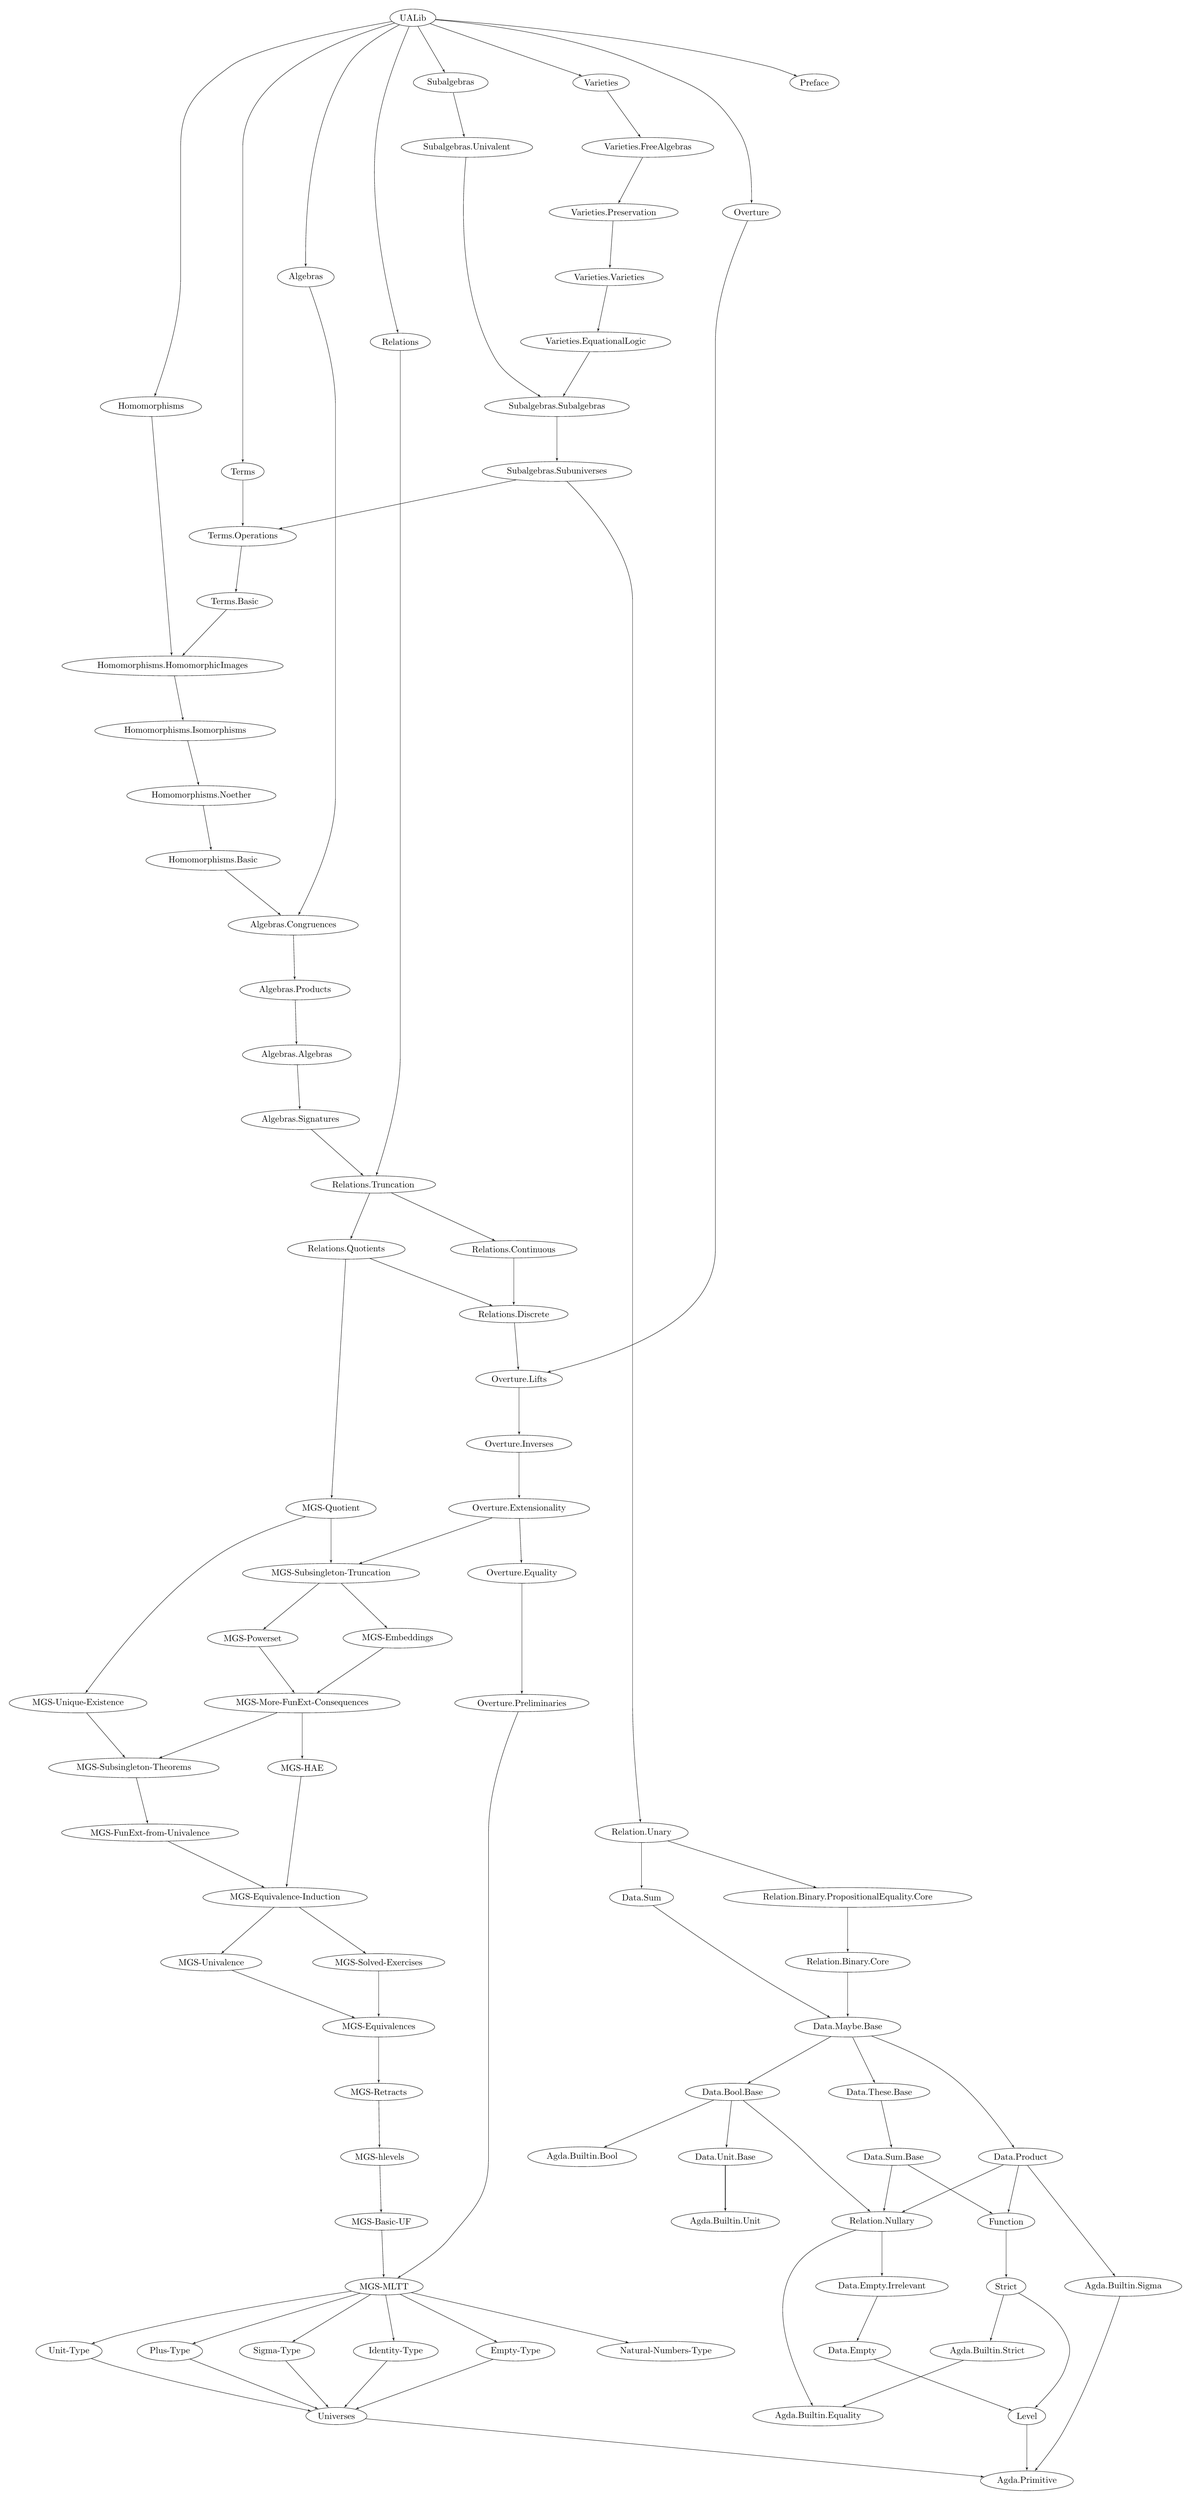
\begin{tikzpicture}[>=latex',line join=bevel]
%%
\node (m80) at (177.19bp,2322.0bp) [draw,ellipse] {Homomorphisms};
  \node (m41) at (686.19bp,2466.0bp) [draw,ellipse] {Varieties.Varieties};
  \node (m20) at (317.19bp,162.0bp) [draw,ellipse] {Sigma-Type};
  \node (m43) at (628.19bp,2322.0bp) [draw,ellipse] {Subalgebras.Subalgebras};
  \node (m33) at (589.19bp,882.0bp) [draw,ellipse] {Overture.Preliminaries};
  \node (m78) at (510.19bp,2682.0bp) [draw,ellipse] {Subalgebras};
  \node (m58) at (951.19bp,522.0bp) [draw,ellipse] {Data.Maybe.Base};
  \node (m11) at (586.19bp,1170.0bp) [draw,ellipse] {Overture.Inverses};
  \node (m10) at (586.19bp,1242.0bp) [draw,ellipse] {Overture.Lifts};
  \node (m13) at (430.19bp,522.0bp) [draw,ellipse] {MGS-Equivalences};
  \node (m12) at (586.19bp,1098.0bp) [draw,ellipse] {Overture.Extensionality};
  \node (m74) at (454.19bp,2394.0bp) [draw,ellipse] {Relations};
  \node (m14) at (430.19bp,450.0bp) [draw,ellipse] {MGS-Retracts};
  \node (m17) at (436.19bp,234.0bp) [draw,ellipse] {MGS-MLTT};
  \node (m16) at (433.19bp,306.0bp) [draw,ellipse] {MGS-Basic-UF};
  \node (m19) at (198.19bp,162.0bp) [draw,ellipse] {Plus-Type};
  \node (m18) at (749.19bp,162.0bp) [draw,ellipse] {Natural-Numbers-Type};
  \node (m23) at (290.19bp,954.0bp) [draw,ellipse] {MGS-Powerset};
  \node (m75) at (844.19bp,2538.0bp) [draw,ellipse] {Overture};
  \node (m55) at (1127.2bp,306.0bp) [draw,ellipse] {Function};
  \node (m54) at (1002.2bp,378.0bp) [draw,ellipse] {Data.Sum.Base};
  \node (m71) at (246.19bp,1818.0bp) [draw,ellipse] {Homomorphisms.Basic};
  \node (m70) at (233.19bp,1890.0bp) [draw,ellipse] {Homomorphisms.Noether};
  \node (m51) at (722.19bp,666.0bp) [draw,ellipse] {Data.Sum};
  \node (m76) at (279.19bp,2250.0bp) [draw,ellipse] {Terms};
  \node (m39) at (337.19bp,1674.0bp) [draw,ellipse] {Algebras.Products};
  \node (m38) at (335.19bp,1746.0bp) [draw,ellipse] {Algebras.Congruences};
  \node (m37) at (339.19bp,1602.0bp) [draw,ellipse] {Algebras.Algebras};
  \node (m36) at (96.191bp,882.0bp) [draw,ellipse] {MGS-Unique-Existence};
  \node (m35) at (377.19bp,1098.0bp) [draw,ellipse] {MGS-Quotient};
  \node (m34) at (394.19bp,1386.0bp) [draw,ellipse] {Relations.Quotients};
  \node (m59) at (986.19bp,450.0bp) [draw,ellipse] {Data.These.Base};
  \node (m32) at (589.19bp,1026.0bp) [draw,ellipse] {Overture.Equality};
  \node (m31) at (451.19bp,954.0bp) [draw,ellipse] {MGS-Embeddings};
  \node (m30) at (176.19bp,738.0bp) [draw,ellipse] {MGS-FunExt-from-Univalence};
  \node (m5) at (580.19bp,1314.0bp) [draw,ellipse] {Relations.Discrete};
  \node (m4) at (580.19bp,1386.0bp) [draw,ellipse] {Relations.Continuous};
  \node (m7) at (383.19bp,90.0bp) [draw,ellipse] {Universes};
  \node (m6) at (582.19bp,162.0bp) [draw,ellipse] {Empty-Type};
  \node (m1) at (349.19bp,2466.0bp) [draw,ellipse] {Algebras};
  \node (m0) at (468.19bp,2754.0bp) [draw,ellipse] {UALib};
  \node (m3) at (424.19bp,1458.0bp) [draw,ellipse] {Relations.Truncation};
  \node (m2) at (343.19bp,1530.0bp) [draw,ellipse] {Algebras.Signatures};
  \node (m52) at (815.19bp,378.0bp) [draw,ellipse] {Data.Unit.Base};
  \node (m53) at (815.19bp,306.0bp) [draw,ellipse] {Agda.Builtin.Unit};
  \node (m9) at (86.191bp,162.0bp) [draw,ellipse] {Unit-Type};
  \node (m8) at (1150.2bp,18.0bp) [draw,ellipse] {Agda.Primitive};
  \node (m73) at (691.19bp,2538.0bp) [draw,ellipse] {Varieties.Preservation};
  \node (m68) at (201.19bp,2034.0bp) [draw,ellipse] {Homomorphisms.HomomorphicImages};
  \node (m72) at (729.19bp,2610.0bp) [draw,ellipse] {Varieties.FreeAlgebras};
  \node (m62) at (1143.2bp,378.0bp) [draw,ellipse] {Data.Product};
  \node (m50) at (1150.2bp,90.0bp) [draw,ellipse] {Level};
  \node (m28) at (244.19bp,594.0bp) [draw,ellipse] {MGS-Univalence};
  \node (m63) at (1257.2bp,234.0bp) [draw,ellipse] {Agda.Builtin.Sigma};
  \node (m56) at (1127.2bp,234.0bp) [draw,ellipse] {Strict};
  \node (m57) at (1106.2bp,162.0bp) [draw,ellipse] {Agda.Builtin.Strict};
  \node (m22) at (377.19bp,1026.0bp) [draw,ellipse] {MGS-Subsingleton-Truncation};
  \node (m77) at (914.19bp,2682.0bp) [draw,ellipse] {Preface};
  \node (m65) at (951.19bp,594.0bp) [draw,ellipse] {Relation.Binary.Core};
  \node (m60) at (823.19bp,450.0bp) [draw,ellipse] {Data.Bool.Base};
  \node (m61) at (656.19bp,378.0bp) [draw,ellipse] {Agda.Builtin.Bool};
  \node (m48) at (989.19bp,234.0bp) [draw,ellipse] {Data.Empty.Irrelevant};
  \node (m49) at (956.19bp,162.0bp) [draw,ellipse] {Data.Empty};
  \node (m64) at (951.19bp,666.0bp) [draw,ellipse] {Relation.Binary.PropositionalEquality.Core};
  \node (m29) at (158.19bp,810.0bp) [draw,ellipse] {MGS-Subsingleton-Theorems};
  \node (m66) at (279.19bp,2178.0bp) [draw,ellipse] {Terms.Operations};
  \node (m67) at (270.19bp,2106.0bp) [draw,ellipse] {Terms.Basic};
  \node (m24) at (345.19bp,882.0bp) [draw,ellipse] {MGS-More-FunExt-Consequences};
  \node (m25) at (345.19bp,810.0bp) [draw,ellipse] {MGS-HAE};
  \node (m26) at (326.19bp,666.0bp) [draw,ellipse] {MGS-Equivalence-Induction};
  \node (m27) at (430.19bp,594.0bp) [draw,ellipse] {MGS-Solved-Exercises};
  \node (m46) at (989.19bp,306.0bp) [draw,ellipse] {Relation.Nullary};
  \node (m47) at (918.19bp,90.0bp) [draw,ellipse] {Agda.Builtin.Equality};
  \node (m44) at (628.19bp,2250.0bp) [draw,ellipse] {Subalgebras.Subuniverses};
  \node (m45) at (722.19bp,738.0bp) [draw,ellipse] {Relation.Unary};
  \node (m42) at (671.19bp,2394.0bp) [draw,ellipse] {Varieties.EquationalLogic};
  \node (m69) at (215.19bp,1962.0bp) [draw,ellipse] {Homomorphisms.Isomorphisms};
  \node (m15) at (431.19bp,378.0bp) [draw,ellipse] {MGS-hlevels};
  \node (m21) at (449.19bp,162.0bp) [draw,ellipse] {Identity-Type};
  \node (m40) at (677.19bp,2682.0bp) [draw,ellipse] {Varieties};
  \node (m79) at (528.19bp,2610.0bp) [draw,ellipse] {Subalgebras.Univalent};
  \draw [->] (m76) ..controls (279.19bp,2224.1bp) and (279.19bp,2215.0bp)  .. (m66);
  \draw [->] (m2) ..controls (373.32bp,1503.2bp) and (385.73bp,1492.2bp)  .. (m3);
  \draw [->] (m56) ..controls (1119.7bp,208.21bp) and (1116.9bp,198.6bp)  .. (m57);
  \draw [->] (m1) ..controls (365.69bp,2421.2bp) and (382.19bp,2368.4bp)  .. (382.19bp,2322.0bp) .. controls (382.19bp,2322.0bp) and (382.19bp,2322.0bp)  .. (382.19bp,1890.0bp) .. controls (382.19bp,1847.7bp) and (363.6bp,1801.6bp)  .. (m38);
  \draw [->] (m44) ..controls (672.04bp,2206.5bp) and (712.19bp,2157.2bp)  .. (712.19bp,2106.0bp) .. controls (712.19bp,2106.0bp) and (712.19bp,2106.0bp)  .. (712.19bp,882.0bp) .. controls (712.19bp,841.78bp) and (716.12bp,795.39bp)  .. (m45);
  \draw [->] (m40) ..controls (695.9bp,2656.1bp) and (703.39bp,2645.7bp)  .. (m72);
  \draw [->] (m0) ..controls (555.0bp,2746.3bp) and (652.29bp,2733.0bp)  .. (728.19bp,2700.0bp) .. controls (779.09bp,2677.9bp) and (800.94bp,2675.2bp)  .. (830.19bp,2628.0bp) .. controls (841.6bp,2609.6bp) and (844.81bp,2585.1bp)  .. (m75);
  \draw [->] (m24) ..controls (274.0bp,854.59bp) and (239.54bp,841.32bp)  .. (m29);
  \draw [->] (m55) ..controls (1127.2bp,280.13bp) and (1127.2bp,270.97bp)  .. (m56);
  \draw [->] (m6) ..controls (511.21bp,136.32bp) and (461.99bp,118.51bp)  .. (m7);
  \draw [->] (m39) ..controls (337.91bp,1648.1bp) and (338.16bp,1639.0bp)  .. (m37);
  \draw [->] (m62) ..controls (1177.1bp,335.19bp) and (1213.7bp,288.88bp)  .. (m63);
  \draw [->] (m5) ..controls (582.35bp,1288.1bp) and (583.11bp,1279.0bp)  .. (m10);
  \draw [->] (m30) ..controls (232.9bp,710.78bp) and (259.23bp,698.14bp)  .. (m26);
  \draw [->] (m3) ..controls (413.34bp,1432.0bp) and (409.43bp,1422.6bp)  .. (m34);
  \draw [->] (m4) ..controls (580.19bp,1360.1bp) and (580.19bp,1351.0bp)  .. (m5);
  \draw [->] (m17) ..controls (534.66bp,211.35bp) and (619.29bp,191.88bp)  .. (m18);
  \draw [->] (m78) ..controls (516.68bp,2656.0bp) and (519.0bp,2646.8bp)  .. (m79);
  \draw [->] (m63) ..controls (1241.0bp,185.14bp) and (1218.2bp,121.54bp)  .. (1190.2bp,72.0bp) .. controls (1184.8bp,62.404bp) and (1177.9bp,52.534bp)  .. (m8);
  \draw [->] (m22) ..controls (344.57bp,999.0bp) and (330.84bp,987.64bp)  .. (m23);
  \draw [->] (m31) ..controls (412.25bp,927.55bp) and (394.9bp,915.76bp)  .. (m24);
  \draw [->] (m34) ..controls (462.9bp,1359.4bp) and (500.97bp,1344.7bp)  .. (m5);
  \draw [->] (m26) ..controls (365.21bp,638.99bp) and (382.08bp,627.31bp)  .. (m27);
  \draw [->] (m16) ..controls (434.27bp,280.13bp) and (434.65bp,270.97bp)  .. (m17);
  \draw [->] (m65) ..controls (951.19bp,568.13bp) and (951.19bp,558.97bp)  .. (m58);
  \draw [->] (m12) ..controls (509.27bp,1071.5bp) and (467.99bp,1057.3bp)  .. (m22);
  \draw [->] (m24) ..controls (345.19bp,856.13bp) and (345.19bp,846.97bp)  .. (m25);
  \draw [->] (m74) ..controls (454.19bp,2348.5bp) and (454.19bp,2295.2bp)  .. (454.19bp,2250.0bp) .. controls (454.19bp,2250.0bp) and (454.19bp,2250.0bp)  .. (454.19bp,1602.0bp) .. controls (454.19bp,1561.1bp) and (442.43bp,1514.9bp)  .. (m3);
  \draw [->] (m10) ..controls (586.19bp,1216.1bp) and (586.19bp,1207.0bp)  .. (m11);
  \draw [->] (m26) ..controls (295.62bp,639.15bp) and (282.94bp,628.03bp)  .. (m28);
  \draw [->] (m71) ..controls (279.4bp,1791.1bp) and (293.19bp,1780.0bp)  .. (m38);
  \draw [->] (m58) ..controls (963.95bp,495.75bp) and (968.65bp,486.08bp)  .. (m59);
  \draw [->] (m7) ..controls (556.19bp,73.76bp) and (921.9bp,39.43bp)  .. (m8);
  \draw [->] (m0) ..controls (382.21bp,2729.3bp) and (279.19bp,2688.0bp)  .. (279.19bp,2610.0bp) .. controls (279.19bp,2610.0bp) and (279.19bp,2610.0bp)  .. (279.19bp,2394.0bp) .. controls (279.19bp,2353.9bp) and (279.19bp,2307.5bp)  .. (m76);
  \draw [->] (m22) ..controls (404.62bp,999.31bp) and (415.83bp,988.4bp)  .. (m31);
  \draw [->] (m58) ..controls (903.52bp,495.19bp) and (880.42bp,482.19bp)  .. (m60);
  \draw [->] (m43) ..controls (628.19bp,2296.1bp) and (628.19bp,2287.0bp)  .. (m44);
  \draw [->] (m3) ..controls (482.38bp,1431.1bp) and (511.41bp,1417.7bp)  .. (m4);
  \draw [->] (m34) ..controls (390.25bp,1319.3bp) and (382.31bp,1184.8bp)  .. (m35);
  \draw [->] (m11) ..controls (586.19bp,1144.1bp) and (586.19bp,1135.0bp)  .. (m12);
  \draw [->] (m29) ..controls (164.68bp,784.05bp) and (167.0bp,774.77bp)  .. (m30);
  \draw [->] (m23) ..controls (310.22bp,927.79bp) and (318.02bp,917.57bp)  .. (m24);
  \draw [->] (m62) ..controls (1088.1bp,352.23bp) and (1057.2bp,337.8bp)  .. (m46);
  \draw [->] (m0) ..controls (483.24bp,2728.2bp) and (489.19bp,2718.0bp)  .. (m78);
  \draw [->] (m13) ..controls (430.19bp,496.13bp) and (430.19bp,486.97bp)  .. (m14);
  \draw [->] (m80) ..controls (182.75bp,2255.3bp) and (193.96bp,2120.8bp)  .. (m68);
  \draw [->] (m38) ..controls (335.91bp,1720.1bp) and (336.16bp,1711.0bp)  .. (m39);
  \draw [->] (m50) ..controls (1150.2bp,64.131bp) and (1150.2bp,54.974bp)  .. (m8);
  \draw [->] (m70) ..controls (237.86bp,1864.1bp) and (239.52bp,1855.0bp)  .. (m71);
  \draw [->] (m19) ..controls (261.91bp,137.2bp) and (307.66bp,119.4bp)  .. (m7);
  \draw [->] (m64) ..controls (951.19bp,640.13bp) and (951.19bp,630.97bp)  .. (m65);
  \draw [->] (m69) ..controls (221.68bp,1936.0bp) and (224.0bp,1926.8bp)  .. (m70);
  \draw [->] (m44) ..controls (499.44bp,2223.4bp) and (407.96bp,2204.6bp)  .. (m66);
  \draw [->] (m20) ..controls (341.36bp,135.64bp) and (351.47bp,124.61bp)  .. (m7);
  \draw [->] (m48) ..controls (977.16bp,207.75bp) and (972.73bp,198.08bp)  .. (m49);
  \draw [->] (m58) ..controls (1015.7bp,497.82bp) and (1043.4bp,484.56bp)  .. (1065.2bp,468.0bp) .. controls (1089.0bp,449.92bp) and (1110.8bp,423.55bp)  .. (m62);
  \draw [->] (m60) ..controls (762.85bp,423.99bp) and (729.26bp,409.5bp)  .. (m61);
  \draw [->] (m14) ..controls (430.55bp,424.13bp) and (430.68bp,414.97bp)  .. (m15);
  \draw [->] (m73) ..controls (689.4bp,2512.1bp) and (688.76bp,2503.0bp)  .. (m41);
  \draw [->] (m57) ..controls (1037.7bp,135.78bp) and (999.94bp,121.31bp)  .. (m47);
  \draw [->] (m0) ..controls (533.9bp,2731.4bp) and (593.98bp,2710.7bp)  .. (m40);
  \draw [->] (m45) ..controls (722.19bp,712.13bp) and (722.19bp,702.97bp)  .. (m51);
  \draw [->] (m35) ..controls (307.23bp,1075.7bp) and (274.22bp,1062.1bp)  .. (248.19bp,1044.0bp) .. controls (192.41bp,1005.3bp) and (141.45bp,943.18bp)  .. (m36);
  \draw [->] (m17) ..controls (392.53bp,207.58bp) and (370.4bp,194.19bp)  .. (m20);
  \draw [->] (m25) ..controls (339.54bp,767.2bp) and (333.74bp,723.25bp)  .. (m26);
  \draw [->] (m0) ..controls (573.55bp,2746.3bp) and (732.86bp,2731.6bp)  .. (863.19bp,2700.0bp) .. controls (867.3bp,2699.0bp) and (871.54bp,2697.8bp)  .. (m77);
  \draw [->] (m0) ..controls (383.67bp,2738.9bp) and (291.86bp,2719.9bp)  .. (265.19bp,2700.0bp) .. controls (227.62bp,2672.0bp) and (210.19bp,2656.9bp)  .. (210.19bp,2610.0bp) .. controls (210.19bp,2610.0bp) and (210.19bp,2610.0bp)  .. (210.19bp,2466.0bp) .. controls (210.19bp,2424.9bp) and (197.25bp,2378.8bp)  .. (m80);
  \draw [->] (m68) ..controls (206.22bp,2008.1bp) and (208.0bp,1999.0bp)  .. (m69);
  \draw [->] (m54) ..controls (997.52bp,352.13bp) and (995.87bp,342.97bp)  .. (m46);
  \draw [->] (m28) ..controls (311.83bp,567.82bp) and (349.99bp,553.05bp)  .. (m13);
  \draw [->] (m62) ..controls (1137.4bp,352.13bp) and (1135.4bp,342.97bp)  .. (m55);
  \draw [->] (m12) ..controls (587.27bp,1072.1bp) and (587.65bp,1063.0bp)  .. (m32);
  \draw [->] (m0) ..controls (450.15bp,2712.1bp) and (433.36bp,2667.8bp)  .. (428.19bp,2628.0bp) .. controls (418.55bp,2553.7bp) and (436.06bp,2465.8bp)  .. (m74);
  \draw [->] (m52) ..controls (815.19bp,352.13bp) and (815.19bp,342.97bp)  .. (m53);
  \draw [->] (m79) ..controls (522.5bp,2550.5bp) and (518.42bp,2447.3bp)  .. (559.19bp,2376.0bp) .. controls (566.11bp,2363.9bp) and (576.92bp,2353.5bp)  .. (m43);
  \draw [->] (m59) ..controls (991.94bp,424.13bp) and (993.97bp,414.97bp)  .. (m54);
  \draw [->] (m37) ..controls (340.63bp,1576.1bp) and (341.14bp,1567.0bp)  .. (m2);
  \draw [->] (m60) ..controls (820.32bp,424.13bp) and (819.3bp,414.97bp)  .. (m52);
  \draw [->] (m60) ..controls (857.95bp,422.45bp) and (874.75bp,408.72bp)  .. (889.19bp,396.0bp) .. controls (906.65bp,380.62bp) and (909.97bp,375.64bp)  .. (927.19bp,360.0bp) .. controls (938.14bp,350.06bp) and (950.38bp,339.32bp)  .. (m46);
  \draw [->] (m42) ..controls (655.41bp,2367.6bp) and (649.49bp,2357.7bp)  .. (m43);
  \draw [->] (m54) ..controls (1049.1bp,350.99bp) and (1073.4bp,336.99bp)  .. (m55);
  \draw [->] (m27) ..controls (430.19bp,568.13bp) and (430.19bp,558.97bp)  .. (m13);
  \draw [->] (m56) ..controls (1165.4bp,213.12bp) and (1184.3bp,198.73bp)  .. (1193.2bp,180.0bp) .. controls (1200.0bp,165.54bp) and (1198.5bp,159.1bp)  .. (1193.2bp,144.0bp) .. controls (1189.2bp,132.57bp) and (1181.7bp,121.74bp)  .. (m50);
  \draw [->] (m46) ..controls (989.19bp,280.13bp) and (989.19bp,270.97bp)  .. (m48);
  \draw [->] (m32) ..controls (589.19bp,983.2bp) and (589.19bp,939.25bp)  .. (m33);
  \draw [->] (m46) ..controls (922.83bp,284.22bp) and (901.68bp,271.36bp)  .. (890.19bp,252.0bp) .. controls (865.13bp,209.78bp) and (886.39bp,151.15bp)  .. (m47);
  \draw [->] (m17) ..controls (489.03bp,207.94bp) and (518.54bp,193.39bp)  .. (m6);
  \draw [->] (m35) ..controls (377.19bp,1072.1bp) and (377.19bp,1063.0bp)  .. (m22);
  \draw [->] (m21) ..controls (425.03bp,135.64bp) and (414.91bp,124.61bp)  .. (m7);
  \draw [->] (m36) ..controls (118.91bp,855.61bp) and (127.92bp,845.15bp)  .. (m29);
  \draw [->] (m75) ..controls (824.19bp,2493.5bp) and (804.19bp,2441.0bp)  .. (804.19bp,2394.0bp) .. controls (804.19bp,2394.0bp) and (804.19bp,2394.0bp)  .. (804.19bp,1386.0bp) .. controls (804.19bp,1310.2bp) and (711.23bp,1272.0bp)  .. (m10);
  \draw [->] (m67) ..controls (245.12bp,2079.8bp) and (234.82bp,2069.1bp)  .. (m68);
  \draw [->] (m9) ..controls (128.61bp,147.89bp) and (135.59bp,145.8bp)  .. (142.19bp,144.0bp) .. controls (206.89bp,126.39bp) and (282.47bp,110.15bp)  .. (m7);
  \draw [->] (m17) ..controls (356.4bp,211.08bp) and (301.11bp,194.91bp)  .. (253.19bp,180.0bp) .. controls (249.93bp,178.98bp) and (246.56bp,177.92bp)  .. (m19);
  \draw [->] (m0) ..controls (426.25bp,2732.0bp) and (406.57bp,2718.0bp)  .. (395.19bp,2700.0bp) .. controls (354.01bp,2634.9bp) and (348.39bp,2540.8bp)  .. (m1);
  \draw [->] (m17) ..controls (324.26bp,217.43bp) and (225.61bp,200.97bp)  .. (142.19bp,180.0bp) .. controls (138.61bp,179.1bp) and (134.93bp,178.1bp)  .. (m9);
  \draw [->] (m49) ..controls (1027.5bp,135.52bp) and (1079.8bp,116.13bp)  .. (m50);
  \draw [->] (m15) ..controls (431.91bp,352.13bp) and (432.16bp,342.97bp)  .. (m16);
  \draw [->] (m66) ..controls (275.96bp,2152.1bp) and (274.81bp,2143.0bp)  .. (m67);
  \draw [->] (m17) ..controls (440.86bp,208.13bp) and (442.52bp,198.97bp)  .. (m21);
  \draw [->] (m41) ..controls (680.8bp,2440.1bp) and (678.89bp,2431.0bp)  .. (m42);
  \draw [->] (m51) ..controls (770.96bp,631.79bp) and (816.16bp,600.78bp)  .. (856.19bp,576.0bp) .. controls (874.16bp,564.88bp) and (894.47bp,553.22bp)  .. (m58);
  \draw [->] (m72) ..controls (715.29bp,2583.7bp) and (710.12bp,2573.9bp)  .. (m73);
  \draw [->] (m45) ..controls (799.66bp,713.64bp) and (848.38bp,698.32bp)  .. (m64);
  \draw [->] (m33) ..controls (570.48bp,836.78bp) and (552.19bp,784.46bp)  .. (552.19bp,738.0bp) .. controls (552.19bp,738.0bp) and (552.19bp,738.0bp)  .. (552.19bp,378.0bp) .. controls (552.19bp,333.67bp) and (537.4bp,322.2bp)  .. (509.19bp,288.0bp) .. controls (499.0bp,275.65bp) and (485.41bp,264.6bp)  .. (m17);
%
\end{tikzpicture}
}
% End of code

% %
% \end{document}
% %





%% \section{Some Components of the Type Topology Library}
%% Here we collect some of the components from the \typetopology library that we used above but did not have space to discuss.  They are collected here for the reader's convenience and to keep the paper somewhat self-contained.

%% \begin{code}
\>[0]\AgdaFunction{transport}%
\>[1275I]\AgdaSymbol{:}\AgdaSpace{}%
\AgdaSymbol{\{}\AgdaBound{X}\AgdaSpace{}%
\AgdaSymbol{:}\AgdaSpace{}%
\AgdaGeneralizable{𝓤}\AgdaSpace{}%
\AgdaOperator{\AgdaFunction{̇}}\AgdaSpace{}%
\AgdaSymbol{\}}\AgdaSpace{}%
\AgdaSymbol{(}\AgdaBound{A}\AgdaSpace{}%
\AgdaSymbol{:}\AgdaSpace{}%
\AgdaBound{X}\AgdaSpace{}%
\AgdaSymbol{→}\AgdaSpace{}%
\AgdaGeneralizable{𝓥}\AgdaSpace{}%
\AgdaOperator{\AgdaFunction{̇}}\AgdaSpace{}%
\AgdaSymbol{)}\AgdaSpace{}%
\AgdaSymbol{\{}\AgdaBound{x}\AgdaSpace{}%
\AgdaBound{y}\AgdaSpace{}%
\AgdaSymbol{:}\AgdaSpace{}%
\AgdaBound{X}\AgdaSymbol{\}}\<%
\\
\>[.][@{}l@{}]\<[1275I]%
\>[10]\AgdaSymbol{→}\AgdaSpace{}%
\AgdaBound{x}\AgdaSpace{}%
\AgdaOperator{\AgdaDatatype{≡}}\AgdaSpace{}%
\AgdaBound{y}\AgdaSpace{}%
\AgdaSymbol{→}\AgdaSpace{}%
\AgdaBound{A}\AgdaSpace{}%
\AgdaBound{x}\AgdaSpace{}%
\AgdaSymbol{→}\AgdaSpace{}%
\AgdaBound{A}\AgdaSpace{}%
\AgdaBound{y}\<%
\\
%
\\[\AgdaEmptyExtraSkip]%
\>[0]\AgdaFunction{transport}\AgdaSpace{}%
\AgdaBound{A}\AgdaSpace{}%
\AgdaSymbol{(}\AgdaInductiveConstructor{refl}\AgdaSpace{}%
\AgdaBound{x}\AgdaSymbol{)}\AgdaSpace{}%
\AgdaSymbol{=}\AgdaSpace{}%
\AgdaFunction{𝑖𝑑}\AgdaSpace{}%
\AgdaSymbol{(}\AgdaBound{A}\AgdaSpace{}%
\AgdaBound{x}\AgdaSymbol{)}\<%
\end{code}
\scpad
\begin{code}
  \>[0]\AgdaFunction{to-Σ-≡}%
\>[1596I]\AgdaSymbol{:}\AgdaSpace{}%
\AgdaSymbol{\{}\AgdaBound{X}\AgdaSpace{}%
\AgdaSymbol{:}\AgdaSpace{}%
\AgdaGeneralizable{𝓤}\AgdaSpace{}%
\AgdaOperator{\AgdaFunction{̇}}\AgdaSpace{}%
\AgdaSymbol{\}}\AgdaSpace{}%
\AgdaSymbol{\{}\AgdaBound{A}\AgdaSpace{}%
\AgdaSymbol{:}\AgdaSpace{}%
\AgdaBound{X}\AgdaSpace{}%
\AgdaSymbol{→}\AgdaSpace{}%
\AgdaGeneralizable{𝓥}\AgdaSpace{}%
\AgdaOperator{\AgdaFunction{̇}}\AgdaSpace{}%
\AgdaSymbol{\}}\AgdaSpace{}%
\AgdaSymbol{\{}\AgdaBound{σ}\AgdaSpace{}%
\AgdaBound{τ}\AgdaSpace{}%
\AgdaSymbol{:}\AgdaSpace{}%
\AgdaRecord{Σ}\AgdaSpace{}%
\AgdaBound{A}\AgdaSymbol{\}}\<%
\\
\>[.][@{}l@{}]\<[1596I]%
\>[7]\AgdaSymbol{→}\AgdaSpace{}%
\AgdaSymbol{(}\AgdaFunction{Σ}\AgdaSpace{}%
\AgdaBound{p}\AgdaSpace{}%
\AgdaFunction{꞉}\AgdaSpace{}%
\AgdaFunction{pr₁}\AgdaSpace{}%
\AgdaBound{σ}\AgdaSpace{}%
\AgdaOperator{\AgdaDatatype{≡}}\AgdaSpace{}%
\AgdaFunction{pr₁}\AgdaSpace{}%
\AgdaBound{τ}\AgdaSpace{}%
\AgdaFunction{,}\AgdaSpace{}%
\AgdaFunction{transport}\AgdaSpace{}%
\AgdaBound{A}\AgdaSpace{}%
\AgdaBound{p}\AgdaSpace{}%
\AgdaSymbol{(}\AgdaFunction{pr₂}\AgdaSpace{}%
\AgdaBound{σ}\AgdaSymbol{)}\AgdaSpace{}%
\AgdaOperator{\AgdaDatatype{≡}}\AgdaSpace{}%
\AgdaFunction{pr₂}\AgdaSpace{}%
\AgdaBound{τ}\AgdaSymbol{)}\<%
\\
%
\>[7]\AgdaSymbol{→}\AgdaSpace{}%
\AgdaBound{σ}\AgdaSpace{}%
\AgdaOperator{\AgdaDatatype{≡}}\AgdaSpace{}%
\AgdaBound{τ}\<%
\\
%
\\[\AgdaEmptyExtraSkip]%
\>[0]\AgdaFunction{to-Σ-≡}\AgdaSpace{}%
\AgdaSymbol{(}\AgdaInductiveConstructor{refl}\AgdaSpace{}%
\AgdaBound{x}\AgdaSpace{}%
\AgdaOperator{\AgdaInductiveConstructor{,}}\AgdaSpace{}%
\AgdaInductiveConstructor{refl}\AgdaSpace{}%
\AgdaBound{a}\AgdaSymbol{)}\AgdaSpace{}%
\AgdaSymbol{=}\AgdaSpace{}%
\AgdaInductiveConstructor{refl}\AgdaSpace{}%
\AgdaSymbol{(}\AgdaBound{x}\AgdaSpace{}%
\AgdaOperator{\AgdaInductiveConstructor{,}}\AgdaSpace{}%
\AgdaBound{a}\AgdaSymbol{)}\<%
\end{code}


\subsubsection{Dependent function extensionality}\label{dependent-function-extensionality}

dfunext : ∀ 𝓤 𝓥 → (𝓤 ⊔ 𝓥)⁺ ̇
dfunext 𝓤 𝓥 = {X : 𝓤 ̇ } {A : X → 𝓥 ̇ } {f g : Π A} → f ∼ g → f ≡ g

global-dfunext : 𝓤ω
global-dfunext = ∀ {𝓤 𝓥} → dfunext 𝓤 𝓥

happly : {X : 𝓤 ̇ } {A : X → 𝓥 ̇ } (f g : Π A) → f ≡ g → f ∼ g
happly f g p x = ap (λ - → - x) p

Extensionality for dependent function types is defined as follows.
\ccpad
\begin{code}%
\>[0]\AgdaFunction{dep-extensionality}\AgdaSpace{}%
\AgdaSymbol{:}\AgdaSpace{}%
\AgdaSymbol{∀}\AgdaSpace{}%
\AgdaBound{𝓤}\AgdaSpace{}%
\AgdaBound{𝓦}\AgdaSpace{}%
\AgdaSymbol{→}\AgdaSpace{}%
\AgdaBound{𝓤}\AgdaSpace{}%
\AgdaOperator{\AgdaPrimitive{⁺}}\AgdaSpace{}%
\AgdaOperator{\AgdaPrimitive{⊔}}\AgdaSpace{}%
\AgdaBound{𝓦}\AgdaSpace{}%
\AgdaOperator{\AgdaPrimitive{⁺}}\AgdaSpace{}%
\AgdaOperator{\AgdaFunction{̇}}\<%
\\
\>[0]\AgdaFunction{dep-extensionality}\AgdaSpace{}%
\AgdaBound{𝓤}\AgdaSpace{}%
\AgdaBound{𝓦}\AgdaSpace{}%
\AgdaSymbol{=}\AgdaSpace{}%
\AgdaSymbol{\{}\AgdaBound{A}\AgdaSpace{}%
\AgdaSymbol{:}\AgdaSpace{}%
\AgdaBound{𝓤}\AgdaSpace{}%
\AgdaOperator{\AgdaFunction{̇}}\AgdaSpace{}%
\AgdaSymbol{\}}\AgdaSpace{}%
\AgdaSymbol{\{}\AgdaBound{B}\AgdaSpace{}%
\AgdaSymbol{:}\AgdaSpace{}%
\AgdaBound{A}\AgdaSpace{}%
\AgdaSymbol{→}\AgdaSpace{}%
\AgdaBound{𝓦}\AgdaSpace{}%
\AgdaOperator{\AgdaFunction{̇}}\AgdaSpace{}%
\AgdaSymbol{\}}\<%
\\
\>[0][@{}l@{\AgdaIndent{0}}]%
\>[2]\AgdaSymbol{\{}\AgdaBound{f}\AgdaSpace{}%
\AgdaBound{g}\AgdaSpace{}%
\AgdaSymbol{:}\AgdaSpace{}%
\AgdaSymbol{∀(}\AgdaBound{x}\AgdaSpace{}%
\AgdaSymbol{:}\AgdaSpace{}%
\AgdaBound{A}\AgdaSymbol{)}\AgdaSpace{}%
\AgdaSymbol{→}\AgdaSpace{}%
\AgdaBound{B}\AgdaSpace{}%
\AgdaBound{x}\AgdaSymbol{\}}\AgdaSpace{}%
\AgdaSymbol{→}%
\>[28]\AgdaBound{f}\AgdaSpace{}%
\AgdaOperator{\AgdaFunction{∼}}\AgdaSpace{}%
\AgdaBound{g}%
\>[35]\AgdaSymbol{→}%
\>[38]\AgdaBound{f}\AgdaSpace{}%
\AgdaOperator{\AgdaDatatype{≡}}\AgdaSpace{}%
\AgdaBound{g}\<%
\end{code}
\ccpad
Sometimes we need extensionality principles that work at all universe levels, and Agda is capable of expressing such principles, which belong to the special 𝓤ω type, as follows:
\ccpad
\begin{code}%
\>[0]\AgdaFunction{∀-extensionality}\AgdaSpace{}%
\AgdaSymbol{:}\AgdaSpace{}%
\AgdaPrimitive{𝓤ω}\<%
\\
\>[0]\AgdaFunction{∀-extensionality}\AgdaSpace{}%
\AgdaSymbol{=}\AgdaSpace{}%
\AgdaSymbol{∀}%
\>[22]\AgdaSymbol{\{}\AgdaBound{𝓤}\AgdaSpace{}%
\AgdaBound{𝓥}\AgdaSymbol{\}}\AgdaSpace{}%
\AgdaSymbol{→}\AgdaSpace{}%
\AgdaFunction{extensionality}\AgdaSpace{}%
\AgdaBound{𝓤}\AgdaSpace{}%
\AgdaBound{𝓥}\<%
\\
%
\\[\AgdaEmptyExtraSkip]%
\>[0]\AgdaFunction{∀-dep-extensionality}\AgdaSpace{}%
\AgdaSymbol{:}\AgdaSpace{}%
\AgdaPrimitive{𝓤ω}\<%
\\
\>[0]\AgdaFunction{∀-dep-extensionality}\AgdaSpace{}%
\AgdaSymbol{=}\AgdaSpace{}%
\AgdaSymbol{∀}\AgdaSpace{}%
\AgdaSymbol{\{}\AgdaBound{𝓤}\AgdaSpace{}%
\AgdaBound{𝓥}\AgdaSymbol{\}}\AgdaSpace{}%
\AgdaSymbol{→}\AgdaSpace{}%
\AgdaFunction{dep-extensionality}\AgdaSpace{}%
\AgdaBound{𝓤}\AgdaSpace{}%
\AgdaBound{𝓥}\<%
\end{code}
\ccpad
More details about the 𝓤ω type are available at \href{https://agda.readthedocs.io/en/latest/language/universe-levels.html#expressions-of-kind-set}{agda.readthedocs.io}.
\ccpad
\begin{code}%
\>[0]\AgdaFunction{extensionality-lemma}\AgdaSpace{}%
\AgdaSymbol{:}%
\>[119I]\AgdaSymbol{∀}\AgdaSpace{}%
\AgdaSymbol{\{}\AgdaBound{𝓘}\AgdaSpace{}%
\AgdaBound{𝓤}\AgdaSpace{}%
\AgdaBound{𝓥}\AgdaSpace{}%
\AgdaBound{𝓣}\AgdaSymbol{\}}\AgdaSpace{}%
\AgdaSymbol{→}\<%
\\
\>[.][@{}l@{}]\<[119I]%
\>[23]\AgdaSymbol{\{}\AgdaBound{I}\AgdaSpace{}%
\AgdaSymbol{:}\AgdaSpace{}%
\AgdaBound{𝓘}\AgdaSpace{}%
\AgdaOperator{\AgdaFunction{̇}}\AgdaSpace{}%
\AgdaSymbol{\}\{}\AgdaBound{X}\AgdaSpace{}%
\AgdaSymbol{:}\AgdaSpace{}%
\AgdaBound{𝓤}\AgdaSpace{}%
\AgdaOperator{\AgdaFunction{̇}}\AgdaSpace{}%
\AgdaSymbol{\}\{}\AgdaBound{A}\AgdaSpace{}%
\AgdaSymbol{:}\AgdaSpace{}%
\AgdaBound{I}\AgdaSpace{}%
\AgdaSymbol{→}\AgdaSpace{}%
\AgdaBound{𝓥}\AgdaSpace{}%
\AgdaOperator{\AgdaFunction{̇}}\AgdaSpace{}%
\AgdaSymbol{\}}\<%
\\
%
\>[23]\AgdaSymbol{(}\AgdaBound{p}\AgdaSpace{}%
\AgdaBound{q}\AgdaSpace{}%
\AgdaSymbol{:}\AgdaSpace{}%
\AgdaSymbol{(}\AgdaBound{i}\AgdaSpace{}%
\AgdaSymbol{:}\AgdaSpace{}%
\AgdaBound{I}\AgdaSymbol{)}\AgdaSpace{}%
\AgdaSymbol{→}\AgdaSpace{}%
\AgdaSymbol{(}\AgdaBound{X}\AgdaSpace{}%
\AgdaSymbol{→}\AgdaSpace{}%
\AgdaBound{A}\AgdaSpace{}%
\AgdaBound{i}\AgdaSymbol{)}\AgdaSpace{}%
\AgdaSymbol{→}\AgdaSpace{}%
\AgdaBound{𝓣}\AgdaSpace{}%
\AgdaOperator{\AgdaFunction{̇}}\AgdaSpace{}%
\AgdaSymbol{)}\<%
\\
%
\>[23]\AgdaSymbol{(}\AgdaBound{args}\AgdaSpace{}%
\AgdaSymbol{:}\AgdaSpace{}%
\AgdaBound{X}\AgdaSpace{}%
\AgdaSymbol{→}\AgdaSpace{}%
\AgdaSymbol{(}\AgdaFunction{Π}\AgdaSpace{}%
\AgdaBound{A}\AgdaSymbol{))}\<%
\\
\>[0][@{}l@{\AgdaIndent{0}}]%
\>[1]\AgdaSymbol{→}%
\>[23]\AgdaBound{p}\AgdaSpace{}%
\AgdaOperator{\AgdaDatatype{≡}}\AgdaSpace{}%
\AgdaBound{q}\<%
\\
\>[1][@{}l@{\AgdaIndent{0}}]%
\>[23]\AgdaComment{-------------------------------------------------}\<%
\\
\>[0][@{}l@{\AgdaIndent{0}}]%
\>[1]\AgdaSymbol{→}%
\>[23]\AgdaSymbol{(λ}\AgdaSpace{}%
\AgdaBound{i}\AgdaSpace{}%
\AgdaSymbol{→}\AgdaSpace{}%
\AgdaSymbol{(}\AgdaBound{p}\AgdaSpace{}%
\AgdaBound{i}\AgdaSymbol{)(λ}\AgdaSpace{}%
\AgdaBound{x}\AgdaSpace{}%
\AgdaSymbol{→}\AgdaSpace{}%
\AgdaBound{args}\AgdaSpace{}%
\AgdaBound{x}\AgdaSpace{}%
\AgdaBound{i}\AgdaSymbol{))}\AgdaSpace{}%
\AgdaOperator{\AgdaDatatype{≡}}\AgdaSpace{}%
\AgdaSymbol{(λ}\AgdaSpace{}%
\AgdaBound{i}\AgdaSpace{}%
\AgdaSymbol{→}\AgdaSpace{}%
\AgdaSymbol{(}\AgdaBound{q}\AgdaSpace{}%
\AgdaBound{i}\AgdaSymbol{)(λ}\AgdaSpace{}%
\AgdaBound{x}\AgdaSpace{}%
\AgdaSymbol{→}\AgdaSpace{}%
\AgdaBound{args}\AgdaSpace{}%
\AgdaBound{x}\AgdaSpace{}%
\AgdaBound{i}\AgdaSymbol{))}\<%
\\
%
\\[\AgdaEmptyExtraSkip]%
\>[0]\AgdaFunction{extensionality-lemma}\AgdaSpace{}%
\AgdaBound{p}\AgdaSpace{}%
\AgdaBound{q}\AgdaSpace{}%
\AgdaBound{args}\AgdaSpace{}%
\AgdaBound{p≡q}\AgdaSpace{}%
\AgdaSymbol{=}\<%
\\
\>[0][@{}l@{\AgdaIndent{0}}]%
\>[1]\AgdaFunction{ap}\AgdaSpace{}%
\AgdaSymbol{(λ}\AgdaSpace{}%
\AgdaBound{-}\AgdaSpace{}%
\AgdaSymbol{→}\AgdaSpace{}%
\AgdaSymbol{λ}\AgdaSpace{}%
\AgdaBound{i}\AgdaSpace{}%
\AgdaSymbol{→}\AgdaSpace{}%
\AgdaSymbol{(}\AgdaBound{-}\AgdaSpace{}%
\AgdaBound{i}\AgdaSymbol{)}\AgdaSpace{}%
\AgdaSymbol{(λ}\AgdaSpace{}%
\AgdaBound{x}\AgdaSpace{}%
\AgdaSymbol{→}\AgdaSpace{}%
\AgdaBound{args}\AgdaSpace{}%
\AgdaBound{x}\AgdaSpace{}%
\AgdaBound{i}\AgdaSymbol{))}\AgdaSpace{}%
\AgdaBound{p≡q}\<%
\end{code}






%%%%%%%%%%%%%%%%%%%%%%%%%%%%%%%%%%%%%%%%%%%%%%%%%%%%%%%%%%%%%%%%%%%%%%%%%%%
\end{document} %%%%%%%%%%%%%%%%%%%%%%%%%%%%%%%%%%%%%%%%%%%%%%%%%%%%%%%%%%%%
%%%%%%%%%%%%%%%%%%%%%%%%%%%%%%%%%%%%%%%%%%%%%%%%%%%%%%%%%%%%%%%%%%%%%%%%%%%

